% This LaTeX document needs to be compiled with XeLaTeX.
\documentclass[10pt]{article}
\usepackage[utf8]{inputenc}
\usepackage{ucharclasses}
\usepackage{graphicx}
\usepackage[export]{adjustbox}
\graphicspath{ {./images/} }
\usepackage{amsmath}
\usepackage{amsfonts}
\usepackage{amssymb}
\usepackage[version=4]{mhchem}
\usepackage{extpfeil}
\usepackage{stmaryrd}
\usepackage{multirow}
\usepackage{fvextra, csquotes}
\usepackage{underscore}
\usepackage[fallback]{xeCJK}
\usepackage{polyglossia}
\usepackage{fontspec}
\IfFontExistsTF{Noto Serif CJK JP}
{\setCJKmainfont{Noto Serif CJK JP}}
{\IfFontExistsTF{STSong}
  {\setCJKmainfont{STSong}}
  {\IfFontExistsTF{Droid Sans Fallback}
    {\setCJKmainfont{Droid Sans Fallback}}
    {\setCJKmainfont{SimSun}}
}}

\setmainlanguage{english}
\setotherlanguages{german, thai, hindi}
\IfFontExistsTF{Noto Serif Thai}
{\newfontfamily\thaifont{Noto Serif Thai}}
{\IfFontExistsTF{Thonburi}
  {\newfontfamily\thaifont{Thonburi}}
  {\IfFontExistsTF{FreeSerif}
    {\newfontfamily\thaifont{FreeSerif}}
    {\IfFontExistsTF{Tahoma}
      {\newfontfamily\thaifont{Tahoma}}
      {\newfontfamily\thaifont{Arial Unicode MS}}
}}}
\IfFontExistsTF{Noto Serif Devanagari}
{\newfontfamily\hindifont{Noto Serif Devanagari}}
{\IfFontExistsTF{Kohinoor Devanagari}
  {\newfontfamily\hindifont{Kohinoor Devanagari}}
  {\IfFontExistsTF{Devanagari MT}
    {\newfontfamily\hindifont{Devanagari MT}}
    {\IfFontExistsTF{Lohit Devanagari}
      {\newfontfamily\hindifont{Lohit Devanagari}}
      {\IfFontExistsTF{FreeSerif}
        {\newfontfamily\hindifont{FreeSerif}}
        {\newfontfamily\hindifont{Arial Unicode MS}}
}}}}
\IfFontExistsTF{CMU Serif}
{\newfontfamily\lgcfont{CMU Serif}}
{\IfFontExistsTF{DejaVu Sans}
  {\newfontfamily\lgcfont{DejaVu Sans}}
  {\newfontfamily\lgcfont{Georgia}}
}
\setDefaultTransitions{\lgcfont}{}
\setTransitionsFor{Thai}{\thaifont}{\lgcfont}
\setTransitionsForDevanagari{\hindifont}{\rmfamily}

\title{Drganic Chemistry-Some Basic Proinciples ared Techniques }

\author{Substituent group\\
$-\mathrm{NO}_{2}$\\
$-\mathrm{CH}_{3}$ $-\mathrm{C}_{2} \mathrm{H}_{5}$\\
$-\mathrm{OCH}_{3}$}
\date{}


\def\AA{\mathring{\mathrm{A}}}

%New command to display footnote whose markers will always be hidden
\let\svthefootnote\thefootnote
\newcommand\blfootnotetext[1]{%
  \let\thefootnote\relax\footnote{#1}%
  \addtocounter{footnote}{-1}%
  \let\thefootnote\svthefootnote%
}

%Overriding the \footnotetext command to hide the marker if its value is `0`
\let\svfootnotetext\footnotetext
\renewcommand\footnotetext[2][?]{%
  \if\relax#1\relax%
    \ifnum\value{footnote}=0\blfootnotetext{#2}\else\svfootnotetext{#2}\fi%
  \else%
    \if?#1\ifnum\value{footnote}=0\blfootnotetext{#2}\else\svfootnotetext{#2}\fi%
    \else\svfootnotetext[#1]{#2}\fi%
  \fi
}

\begin{document}
\maketitle
\begin{center}

\includegraphics[max width=\textwidth]{2025_01_28_8470952b98110cec3aabg-001}
\end{center}

It's not that I'm so smart, it's just that I stay with problems longer.

\section*{THE BEST}
\section*{STUDY PACKAGE}
\section*{IIT-JEE, AIEEE, NEET, ISEET}
\section*{IIT ACADEMY}
If I have ever made any valuable discoveries, it has been owing more to patient attention than to any other talent.

\section*{STUDY PACKAGE}
\begin{center}
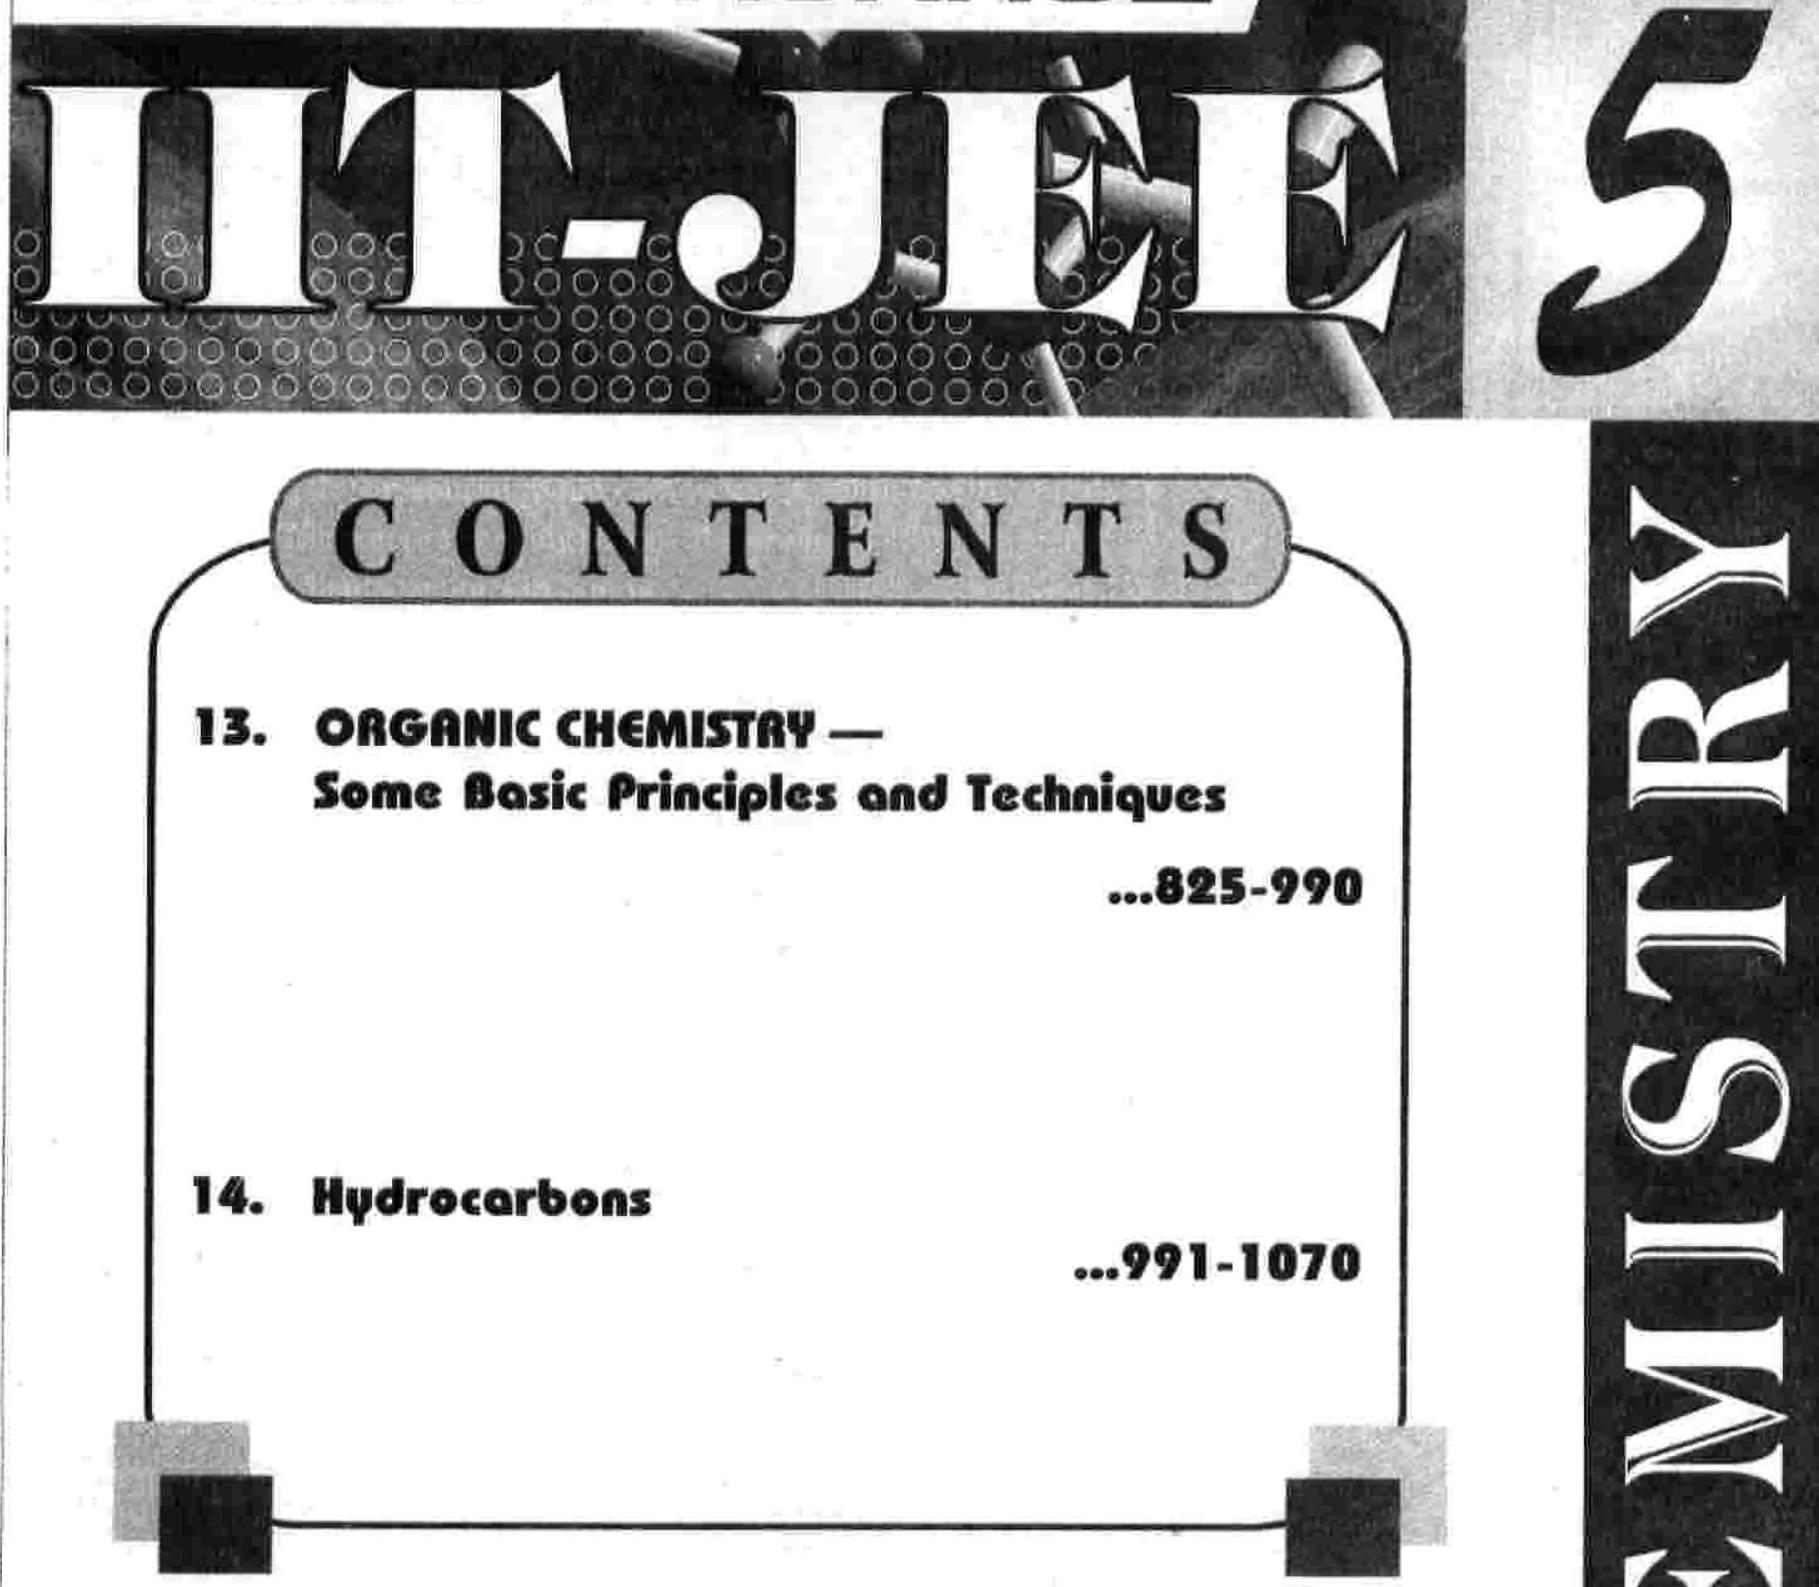
\includegraphics[max width=\textwidth]{2025_01_28_8470952b98110cec3aabg-002}
\end{center}

NAME OF THE STUDENT : $\qquad$

ADDRESS : $\qquad$

PHONE NO. : $\qquad$

EXAM PREPARING FOR : $\qquad$\\
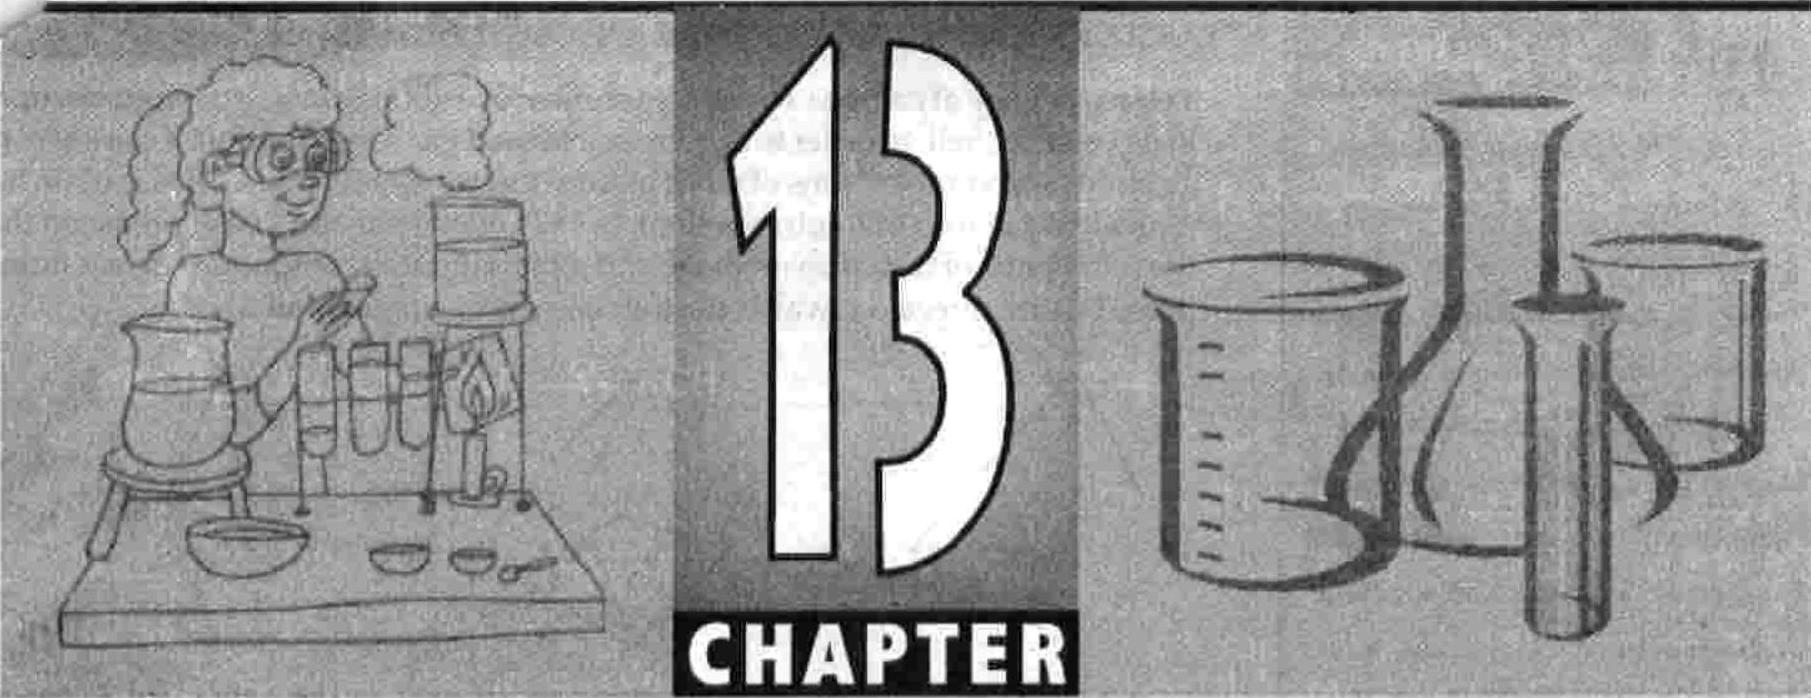
\includegraphics[max width=\textwidth, center]{2025_01_28_8470952b98110cec3aabg-003(1)}

\section*{INTRODUCTION}
Organic chemistry is the study of the preparation, properties, identification, and reactions of those compounds of carbon not classified as inorganic. The latter include the oxide of carbon, the bicarbonates and carbonates of metal ions, the metal cyanides, and a handful of other compounds. There are several million known carbon compounds, and all but a very few are organic.\\
Virtually all plastics, synthetic and natural fibers, dyes and drugs, insecticides and herbicides, ingredients in perfumes and flavouring agents and all petroleum products are organic compounds. All the foods you eat consist chiefly of organic compounds in the famifies of the carbohydrates, fats and oils, proteins, and vitamins. The substances that make up furs and feathers, hides and skins, and all cell membranes are also organic.\\
Originally, the distinction between inorganic and organic substances was based on whether or not they were produced by living systems. For example, until the earty nineteenth century, it was believed that organic compounds had some sort of "life force" and could only be synthesized by living organisms. The view was dispelled in 1828 when German chemist Friedrich Wohler prepared urea from the inorganic salt ammonium cyanate by simple heating :\\
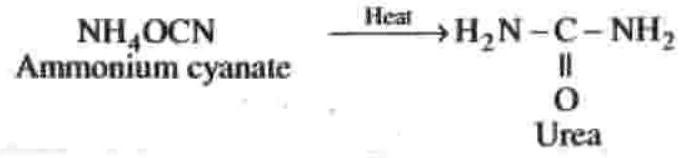
\includegraphics[max width=\textwidth, center]{2025_01_28_8470952b98110cec3aabg-003}

Since urea is a component of urine, it is clearly an organic material, yet there was clear evidence that it could be produced in the laboratory as well as by living things.

\section*{JILC Sylabus}
Concepts: Hylvidisation of farbon: Sigma and pr:bonds; Shapes of simple organic molecules; Stricural and geometrical isomerism: Optical isomerismofiompounds containing up to two asymmetric caltrs, (RS and EZ nomenclaturexaduded); IUPAC nomendature of simple organic compounds (only lyydrociubons, mono functional and bifundtonal compounds); Conformations of cthunc and budame (Nowman projections); Resonance and hypercomingation; Kelo-enol tautomerism; Detimmination ofompinical and molecalar formulac of simple compounds (only combustion method); Hydroger bonds: definition and their effocts on plysical properties of alcohols and carboxylicacids; Inductiveand resonancerffects on acidity and basicily oforganicacids and bases; Polarity and indudive effocts in alkyl halides; Reative internediates produced during homolyficand\\
hetconlytic bond deavagc; Fornation,\\
structureandstability of carbocations, carhanions and frecradicals

\section*{STRUCTURE AND SHAPES OF ORGANICMOLECULES:}
\begin{enumerate}
  \item Tetracovalency of carbon: The atomic number of carbon is 6 and it has four electrons in its valence shell. In order to acquire stable inert gas configuration, it can share its electrons with the electrons of other to form four covalent bonds. Thus, carbon has a covalency of four or is tetracovalent. In 1874, Vant Hoff and Le Bel predicted that the four bonds of carbon in methane and other saturated compounds do not lie in a plane but are directed towards the four corners of a regular tetrahedral.\\
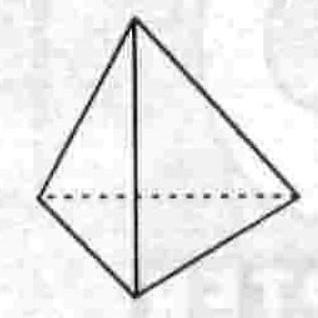
\includegraphics[max width=\textwidth, center]{2025_01_28_8470952b98110cec3aabg-004(1)}
\end{enumerate}

A Regular\\
Tetrahedron with 4 Similar Faces\\
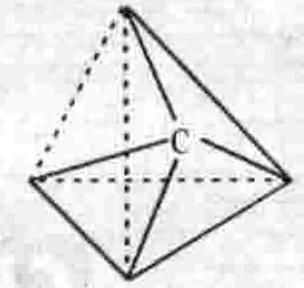
\includegraphics[max width=\textwidth, center]{2025_01_28_8470952b98110cec3aabg-004(2)}

Space Model of Carbon A tom\\
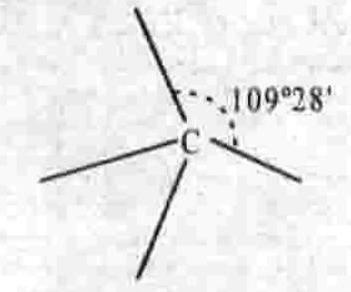
\includegraphics[max width=\textwidth, center]{2025_01_28_8470952b98110cec3aabg-004}

The Normal Direction of Valencies

\section*{Figure : Tetrahedral representation of carbon valencies}
\begin{enumerate}
  \setcounter{enumi}{1}
  \item Formation of organic molecules : We know that organic compounds are carbon compounds and carbon atom does not take part as such in bond formation but its $2 s$ and $2 p$ orbital(s) mix together to form new orbitals known as hybrid orbitals and the process in turn is known as hybridization. The types of hybridizations encountered in organic compounds are $s p^{3}$ (involved in saturated organic compounds containing only single covalent bonds, eg. methane), $s p^{2}$ (involved in organic compounds having carbon linked by double bonds, e.g. ethylene) and $s p$ (involved in organic compounds having carbon linked by a triple bond, e.g acetylenes). The bond angles and geometry associated with the three types of hybridization are summarized below:
\end{enumerate}

\begin{center}
\begin{tabular}{|c|c|c|c|}
\hline
Hybridisation & $s p^{3}$ & $s p^{2}$ & -7p \\
\hline
Angle & $109{ }^{\circ} 28^{\prime}$ & $120^{\circ}$ & $180^{\circ}$ \\
\hline
Geometry & Tetrahedral & Trigonal & Linear \\
\hline
Example & Alkane, Cycloalkane and in saturated part of all organic molecules & Alkenes and other compounds containing $\mathrm{C}=\mathrm{C}, \mathrm{C}=\mathrm{O}$. $\mathrm{C}=\mathrm{N}$ and $\mathrm{C}=\mathrm{S}$ double bonds & Alkynes and all other compounds containing $\mathrm{C} \equiv \mathrm{C}$ and $\mathrm{C} \equiv \mathrm{N}$ triple bonds \\
\hline
Bond & Four- $\sigma$ & Three- $\sigma$, One- $\pi$ & Two- $\sigma$, Two- $\pi$ \\
\hline
$x^{\%}$ & 25 & 33.3 & 1 50 \\
\hline
$p^{2}$ & 75 & 66.7 & $50 . \square$ \\
\hline
Electronegativity & 2.48 & 2.75 & . 3.25 \\
\hline
\end{tabular}
\end{center}

\begin{enumerate}
  \setcounter{enumi}{2}
  \item Types of bonds : Organic compounds normally contain only two types of carbon-carbon bonds, i.e, $\sigma$-(sigma) and $\pi$-(pi).\\
(i) Sigma bond:\\
(a) A carbon-carbon, $\sigma$-bond can be formed by overlap of two $s p^{3}, s p^{2}$ or $s p$-hybridized orbitals of carbon atoms.
\end{enumerate}

Alkanes and cycloalkanes contain only $s p^{3} \rightarrow s p^{3} \mathrm{C}-\mathrm{C}, \sigma$-bonds, alkenes contains $s p^{2}-s p^{2}, \mathrm{C}-\mathrm{C} \sigma$-bonds while alkynes contain $s p-s p, \mathrm{C}-\mathrm{C}, \sigma$-bonds.\\
(b) In a similar way, carbon can form sigma bonds with hydrogen atoms, while alkanes contain only $\mathrm{sp}^{3}-\mathrm{s}, \mathrm{C}-\mathrm{H} \sigma-$ bonds, alkenes contain $s p^{2}-s \mathrm{C}-\mathrm{H}, \sigma$-bonds and alkynes contain $\mathrm{sp}-\mathrm{s} \mathrm{C}-\mathrm{H}, \sigma$-bonds.\\
(ii) $\pi$-bond :\\
(a) A pi-bond is formed by sideways or lateral overlap of two $p$-orbitals, Thus, alkenes contain one $s p^{2}-s p^{2}, \mathrm{C}-\mathrm{C}$, $\sigma$-bond and one $\pi$-bond.\\
(b) In alkynes, the carbon atoms are $s p$-hybridized. Therefore, alkynes contain one $s p-s p, \mathrm{C}-\mathrm{C}, \sigma$-bond and two $\pi-$ bonds which are mutually perpendicular to each other.\\
(c) The two carbon atoms and two hydrogen atoms of acetylene molecule lie along a line with $\mathrm{C}-\mathrm{C}$ bond angle of $180^{\circ}$. Thus, acetylene is a linear molecule.\\
4. Effect of hybridization on bond length and bond strength : The bond length and bond strength of any bond depends upon the size of the hybrid orbitals involved.\\
(i) Bond lengths : Since a $p$-orbital is much bigger in size than a s-orbital of the same shell, therefore, as we go from $s p^{3}$ $\rightarrow s p^{2} \rightarrow s p$, the percentage of $p$-character decreases from $75 \rightarrow 66.7 \rightarrow 50 \%$.\\
Accordingly, the size of the orbital decreases in the same order: $s p^{3}>s p^{2}>s p$.\\
Since a bigger orbital forms a longer bond, therefore, $\mathrm{C}-\mathrm{C}$ single bond lengths decrease in the order:

$$
\begin{gathered}
\mathrm{C}\left(s p^{3}\right)-\mathrm{C}\left(s p^{3}\right) \\
1.54 \AA \\
\mathrm{C}\left(s p^{2}\right)-\mathrm{C}\left(s p^{2}\right) \\
1.34 \AA \\
1.20 \AA \mathrm{C}(s p)-\mathrm{C}(s p)
\end{gathered}
$$

(ii) Bond strengths:

Shorter the bond, greater is its strength. Thus, the $\sigma$-bond formed by sp-hybridized carbon is the strongest (i.e. maximum bond energy) while that formed by $s p^{3}$-hybridized carbon is the weakest (i.e. minimum bond dissociation energy). For example,

\begin{center}
\begin{tabular}{|c|c|c|}
\hline
$\mathrm{C}(\mathrm{sp})-\mathrm{H}$ & $\mathrm{C}\left(s p^{2}\right)-\mathrm{H}>$ & $\mathrm{C}\left(s p^{3}\right)-\mathrm{H}$ \\
\hline
$121 \mathrm{kcal}^{\text {mol }}{ }^{-1}$ & $106 \mathrm{kcal}_{\mathrm{mol}}{ }^{-1}$ & $98.6 \mathrm{kcal} \mathrm{mol}^{-1}$ \\
\hline
$\mathrm{C}(\mathrm{sp})-\mathrm{C}(\mathrm{sp})>$ & $C\left(s p^{2}\right)-\mathrm{C}\left(s p^{2}\right)$ & $C\left(s p^{3}\right)-C\left(s p^{3}\right)$ \\
\hline
$200 \mathrm{kcal}^{\text {mol }}$-1 & $142 \mathrm{kcal}_{\text {mol }}{ }^{-1}$ & $80-85 \mathrm{kcal}_{\text {mol }}{ }^{-1}$ \\
\hline
\end{tabular}
\end{center}

Since the extent of overlap in sideways overlap is low, a carbon-carbon $\pi$-bond is always weaker than a carboncarbon $\sigma$-bond. A carbon-carbon double bond is, however, stronger than a carbon-carbon single bond since it consists

\begin{itemize}
  \item of a stronger $\sigma$-bond and a weak $\pi$-bond. In a similar way, a carbon-carbon triple bond is still stronger than carboncarbon double bond.
\end{itemize}

\begin{enumerate}
  \setcounter{enumi}{4}
  \item Types of carbon and hydrogen atoms : There are four types of carbon atoms :\\
(i) A primary $\left(1^{\circ}\right)$ carbon atom is bonded to either one more carbon atom or to none.\\
(ii) A secondary ( $2^{\circ}$ ) carbon atom is bonded to two other carbon atoms.\\
(iii) A tertiary $\left(3^{\circ}\right)$ carbon atom is bonded to three other carbon atoms.\\
(iv) A quaternary $\left(4^{\circ}\right)$ carbon atom is bonded to four other carbon atoms.
\end{enumerate}

The $1^{\circ}, 2^{\circ}, 3^{\circ}$ and $4^{\circ}$ carbon and $1^{\circ}, 2^{\circ}$ and $3^{\circ}$ hydrogen atoms are illustrated below :\\
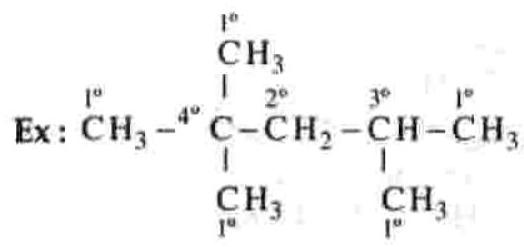
\includegraphics[max width=\textwidth, center]{2025_01_28_8470952b98110cec3aabg-005}

\section*{STRUCTURAL REPRESENTATION OF ORGANIC COMPOUNDS:}
The structures of organic compounds can be represented in several ways. Commonly used methods to describe the structure of any organic compound are :\\
(a) Lewis formula (or Electronic formula) of a compound: The formula showing the mode of electron-sharing between different atoms in the molecule of a compound is called its electronic formula or Lewis formula.\\
Writing of the Lewis formula is primarily based on the octet rule (with certain exceptions).\\
To construct the Lewis formula for a molecule proceed as follows:\\
(i) Determine the total number of available outer electrons in the atoms that make up that molecule,\\
(ii) Arrange these electrons around the atoms so that each atom (except hydrogen) is surrounded by eight electrons (leave aside a few exceptions). The shared electrons are common to the two atoms. Hydrogen atom in any compound will have only two electrons.\\
$\mathrm{CH}_{4}:{ }_{6} \mathrm{C}$ contributes four electrons to bonding, each ${ }_{1} \mathrm{H}$ contributes one electron\\
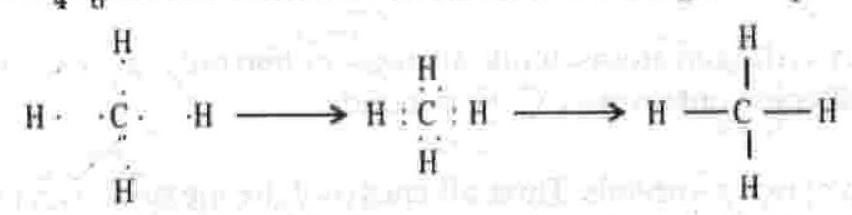
\includegraphics[max width=\textwidth, center]{2025_01_28_8470952b98110cec3aabg-006(1)}

In acetylene (HCCH), for each carbon, two of the four bonding electrons are used in forming single bonds to one hydrogen and the other carbon. Two electrons are left over on each carbon, and these are shared to create a triple bond between the carbons.\\
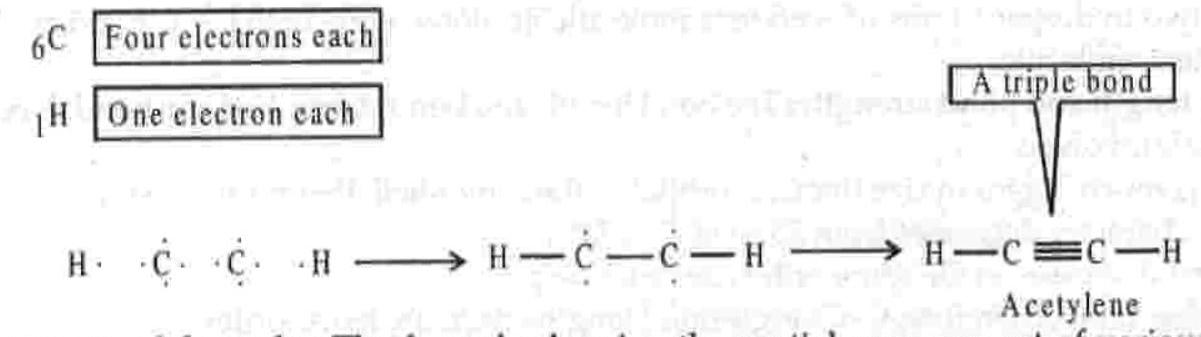
\includegraphics[max width=\textwidth, center]{2025_01_28_8470952b98110cec3aabg-006}\\
(b) Structural formula : The formula showing the spatial arrangement of various atoms present in a molecule of the compound is called its structural formula. In other words, the formula showing the way various atoms are linked to each other in a molecule of any compound is called its structural formula. In structural formula, single bonds are shown by single lines $(-)$, double bonds are shown by double lines $(=)$, and triple bonds by three lines $(\xi)$. Such structural formulae are also called complete structural formulae. Thus, structural formula of a compound is its electronic formula in which one pair of shared electrons (.. or $x \cdot$ ) is replaced by a single bond, two pairs of the shared electrons (: : or : ${ }_{x}^{x}$ ) by a double bond, and three pairs of the shared electrons\\
(: $:$ or $\left.\sum_{x}^{x}\right)$ by a triple bond.\\
(c) Condensed structural formula : Structures can be abbreviated by omitting some or all of the covalent bonds and indicating the number of identical groups attached to an atom by a subscript. Such a compact formula is called condensed structural formula or simply as condensed formula. Thus methane can be represented as $\mathrm{CH}_{4}$ ethane as $\mathrm{CH}_{3}-\mathrm{CH}_{3}$.\\
(d) Bond line structural formula : Writing structural formulae for big complex organic molecule is both time and space consuming. Bond-line notation is a simple and convenient method of describing organic molecules. In this method.\\
(i) Bonds are represented by lines. Thus, single line $(-)$ represents a single bond, two parallel lines $(=)$ represent a double bond, and three parallel lines ( $\equiv$ ) represent a triple bond.\\
(ii) Carbon atoms are represented by the line-ends and line-intersections.

The termini denote a methyl group $\left(-\mathrm{CH}_{3}\right)$ unless indicated, otherwise by a functional group.\\
(iii) Functional group or any substituent may be shown at the appropriate place by using its symbol or formula.\\
(iv) Hydrogen atoms are assumed to be present in the required number so as to satisfy the tetravalency of carbon.

The bond-line structure for common compounds :\\
Cethane\\
(e) Three-dimensional representation : Covalent bonds are directional. Thus, bonds in an organic compound are oriented at certain angles to each other. The three-dimensional (3-D) structures of organic molecules cannot be visualized from two-dimensional structures written on paper. However, structures of the three-dimensional organic molecules can be shown on paper by using solid and dashed wedge method of describing organic molecules.\\
The following conventions are followed while writing solid and dashed wedge formulae.\\
(i) The solid wedge ( $\Delta$ ) is used to describe a bond projecting from the plane of the paper towards the observer.\\
(ii) The dashed wedge ( $V$ ) is used to describe a bond below the plane of the paper away from the observer.\\
(iii) The bond lying in the plane of the paper is shown by a normal line bond.

The solid and dashed wedge formula of methane is:\\
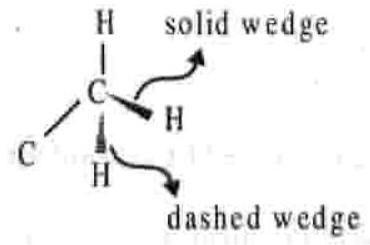
\includegraphics[max width=\textwidth, center]{2025_01_28_8470952b98110cec3aabg-007}

\section*{CLASSIFICATION OF ORGANIC COMPOUNDS:}
\begin{center}
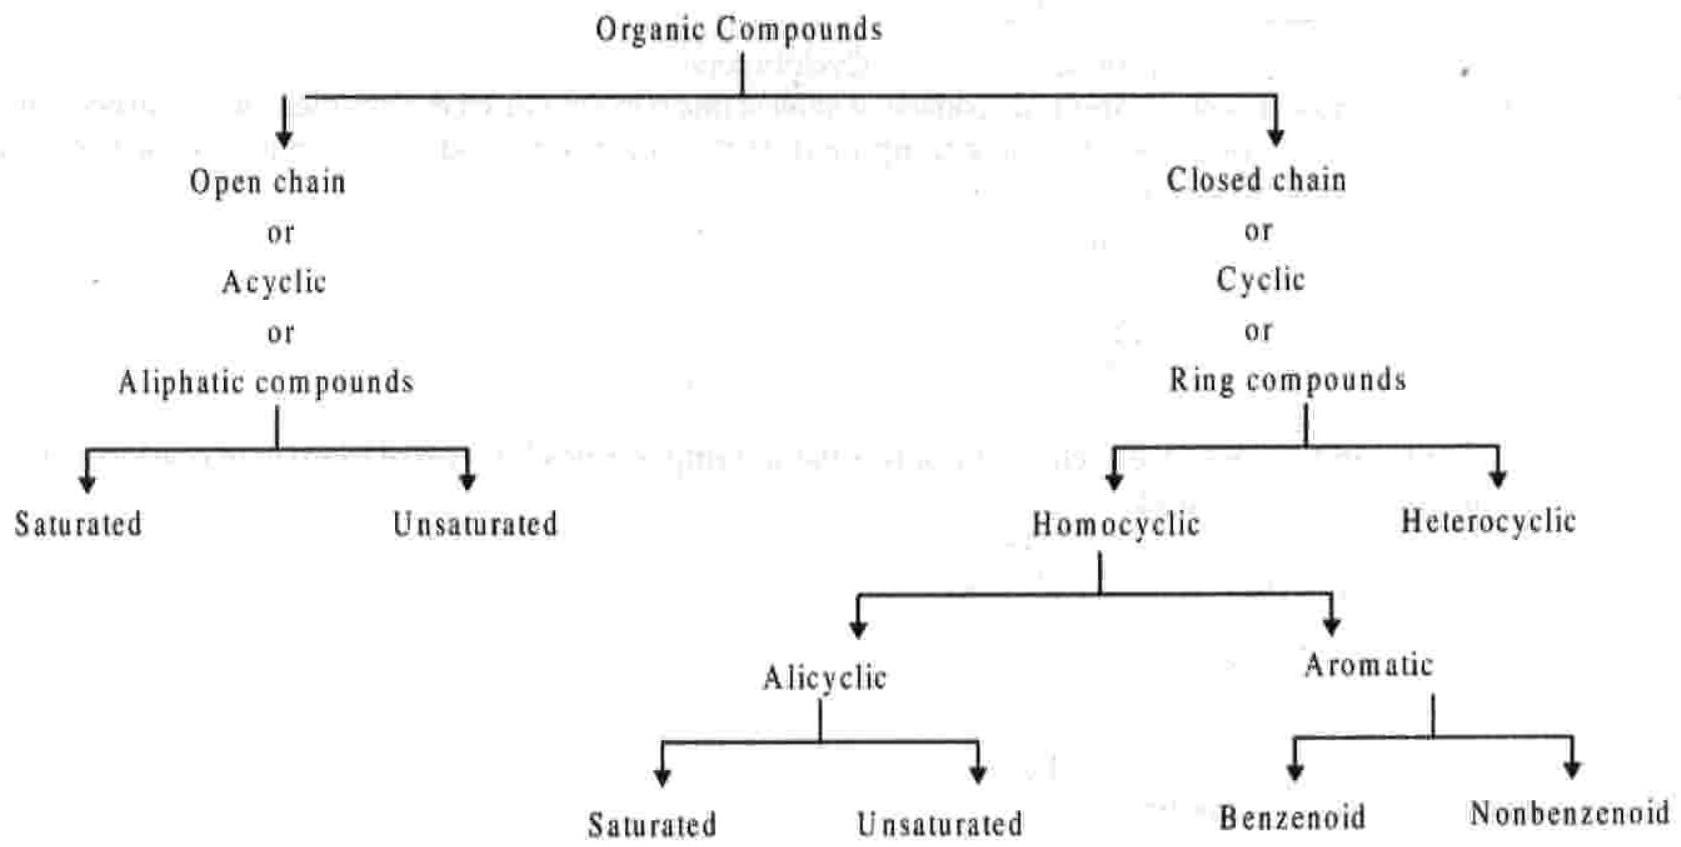
\includegraphics[max width=\textwidth]{2025_01_28_8470952b98110cec3aabg-007(2)}
\end{center}

Aliphatic or open chain compounds : Those compounds in which first and last carbon atoms are not connected with each other. Branched or unbranched chains are possible in these compounds.\\
For example :\\
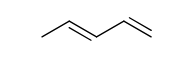
\includegraphics{smile-4d35931270aae4e49a9ba7f56de7f2ac85550e62}\\
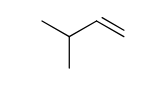
\includegraphics{smile-b3cab2cff8c2699cc45fe98b10f58bec3cf0d742}\\
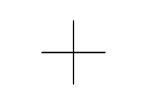
\includegraphics{smile-97a92a886a7faa7c96c9698b5f061d0f3c2713fb}\\
(unbranched)\\
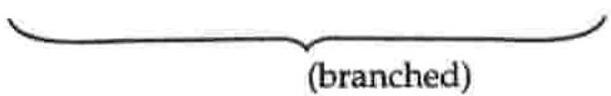
\includegraphics[max width=\textwidth, center]{2025_01_28_8470952b98110cec3aabg-007(1)}

There are two varieties in these compounds-

\section*{Saturated hydrocarbons :}
(a) In such type, adjacent carbons are attached with single bonds.

Ex. $\mathrm{CH}_{3}-\mathrm{CH}_{2}-\mathrm{CH}_{3}$\\
(b) General formula of these compounds is $\mathrm{C}_{n} \mathrm{H}_{2 n+2}$ (alkane)\\
(c) These are also called as paraffins (Parum + Affinis i.e. little reactivity) because these are less reactive due to absence of $\pi$-bonds.

\section*{Unsaturated hydrocarbons:}
(a) There will be a double bond or a triple bond between any two carbons atoms.

$$
\begin{aligned}
& \mathrm{CH}_{2}=\mathrm{CH}-\mathrm{CH}_{3}, \quad \mathrm{CH} \equiv \mathrm{C}-\mathrm{CH}_{3} \\
& \text { Propene }
\end{aligned} \quad \text { Propyne }
$$

(b) General formula is $\mathrm{C}_{n} \mathrm{H}_{2 n}$ and $\mathrm{C}_{n} \mathrm{H}_{2 n-2}$\\
(c) Alkenes are also called as olefins because they react with halogens to form oily substances (Oleum + fenes i.e. Oil forming).\\
(d) Due to presence of $\pi$ bonds, these are more reactive

Cyclic or closed chain compounds : In these compounds first and last carbons are attached with each other.\\
Ex.\\
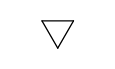
\includegraphics{smile-e7e535da4867be6021ec01f95784b3fbb92929db}

Cyclopropane.\\
These are of two types\\
Homocyclic compounds: These are the compounds in which complete ring is formed by carbon atoms only. These are also of two types.\\
(a) Alicyclic compounds : These are the compounds having the properties like aliphatic compounds. These may be saturated or unsaturated like aliphatic compounds.\\
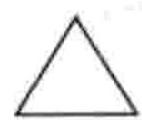
\includegraphics[max width=\textwidth, center]{2025_01_28_8470952b98110cec3aabg-008(2)}

Cyclopropane\\
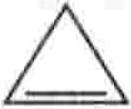
\includegraphics[max width=\textwidth, center]{2025_01_28_8470952b98110cec3aabg-008(3)}

Cyclopropene\\
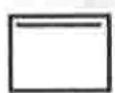
\includegraphics[max width=\textwidth, center]{2025_01_28_8470952b98110cec3aabg-008}\\
(b) Aromatic compounds : These compounds consist of at least one benzene ring i.e. a six-membered carbocyclic ring having alternate single and double bonds. These compounds have some fragrant odour and hence, named as aromatic (greek word aroma means sweet smell)

Ex.\\
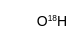
\includegraphics{smile-3bb19601986b44018fefc1e913d04c6d62757666}

Benzene\\
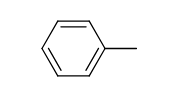
\includegraphics{smile-4dd4fcd25dd7941ce42ac797c95a69325091235d}

Toluen\\
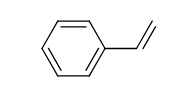
\includegraphics{smile-b6896f1ac27926901a647e747eb8794a5fed872a}

Styrene

Heterocyclic compounds: These are cyclic compounds having ring or rings built up of more than one kind of atoms. (i) Aromatic heterocyclic compounds:\\
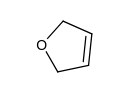
\includegraphics{smile-9cbae8d5125cbb289b0a7eff2c8662600611a900}

0

Furan\\
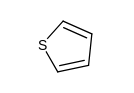
\includegraphics{smile-973b47a7aac7ee80f3b67534bec681239d52a03e}

Thiophene\\
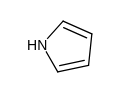
\includegraphics{smile-ea8e0f86c256c71badee4915a8d503c76dca70a2}

Pyrrole\\
(ii) Aliphatic heterocyclic compounds :\\
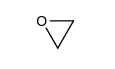
\includegraphics{smile-531b6b3f236341a3a4ca3a32a7f85321f69d5c97}\\
Oxirane or Epoxyethane or Ethylene oxide\\
or Dimethyleue oxide or Oxocyclopropune\\
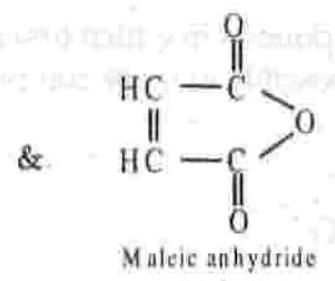
\includegraphics[max width=\textwidth, center]{2025_01_28_8470952b98110cec3aabg-008(1)}

Groups : Atom or a group of atoms which possess any 'charge' on it or any 'free valency' are called as groups. Normal group:\\
(a) It is represented by ' $n$ '.\\
(b) Straight chain of carbon atoms is known as normal group.\\
(c) Free bond will come either on Ist carbon atom or on last carbon atom.\\
n-butyl\\
$\mathrm{C}-\mathrm{C}-\mathrm{C}-\mathrm{C}-$\\
n-propyl\\
$\mathrm{C}-\mathrm{C}-\mathrm{C}-$

Iso group:\\
(a) It is represented by following structure: $\mathrm{H}_{3} \mathrm{C}-\underset{\mid}{\mathrm{CH}}-$\\
(b) When two methyl groups are attached to the same carbon atom, group is named as iso ;\\
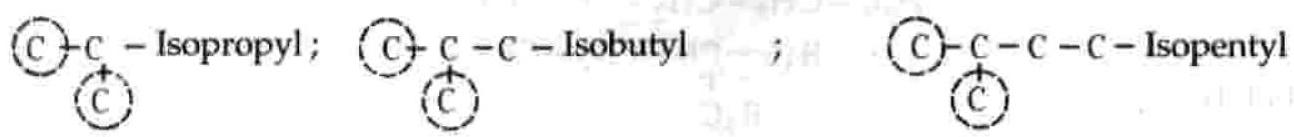
\includegraphics[max width=\textwidth, center]{2025_01_28_8470952b98110cec3aabg-009}

\section*{Secondary group :}
(a) It is represented by following structure $-\mathrm{C}-\mathrm{C}-\mathrm{C}-$\\
(b) When ethyl and methyl groups attached to the terminal carbon atom, group is named as secondary-

Ex. $\underset{C}{C-C} \rightarrow C-$ secondary butyl

\section*{Tertiary group :}
(a) It is represented by following structure $-\mathrm{C}-\mathrm{C}_{\mathrm{C}}^{\mathrm{C}}$\\
(b) When three alkyl groups (similar or dissimilar) are attached to the same carbon atom, group is named as tertiary.\\
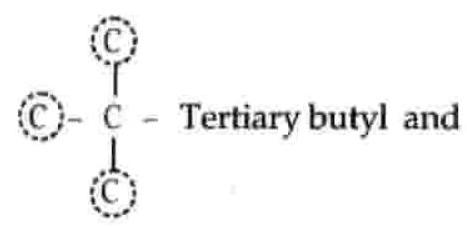
\includegraphics[max width=\textwidth, center]{2025_01_28_8470952b98110cec3aabg-009(2)}\\
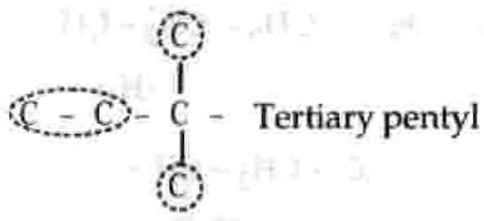
\includegraphics[max width=\textwidth, center]{2025_01_28_8470952b98110cec3aabg-009(3)}

\section*{Neo group:}
(a) When a carbon atom is attached to other four carbon atoms, group is named as neo group.\\
(b) It is represented by following structure :\\
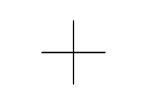
\includegraphics{smile-3c23584335d63d223fc68d5740b5ad2a54044443}\\
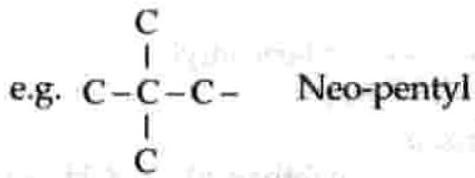
\includegraphics[max width=\textwidth, center]{2025_01_28_8470952b98110cec3aabg-009(1)}

Alkyl group: When a hydrogen is removed from saturated hydrocarbon then alkyl group is formed. It is represented by R and its general formula is $\mathrm{C}_{n} \mathrm{H}_{2 n+1}$. A bond is vacant on alkyl group on which any functional group may come.

$$
\begin{aligned}
& \mathrm{CH}_{4} \xrightarrow[-\mathrm{H}]{ } \mathrm{CH}_{3}-\text { Methyl } \\
& \mathrm{CH}_{3}-\mathrm{CH}_{3} \xrightarrow[-\mathrm{H}]{ } \mathrm{CH}_{3}-\mathrm{CH}_{2}-\text { Ethyl }
\end{aligned}
$$

(a) $\mathrm{C}_{3} \mathrm{H}_{7}$ can be represented as :\\
(i) Normal propyl\\
(ii) Isopropyl (1-methylethyl)\\
(b) $\mathrm{C}_{4} \mathrm{H}_{9}$ can be represented as :\\
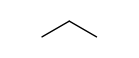
\includegraphics{smile-75aa6e93f5fdf6929b2c1b70472d597d21d35bde}\\
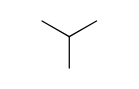
\includegraphics{smile-133c33ba23c66a493bce57678208596a1cb9ec13}\\
(i) $n$-Butyl\\
(ii) Iso butyl (2-methylpropyl)\\
(iii) Secondary butyl (1-methylpropyl)\\
(iv) Tertiary butyl (1,1-dimethylethyl)\\
$\mathrm{H}_{3} \mathrm{C}-\mathrm{CH}_{2}-\mathrm{CH}_{2}-\mathrm{CH}_{2}-$\\
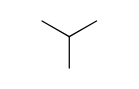
\includegraphics{smile-6a8070635c622907c0602f1cd2d5385829cba4b5}\\
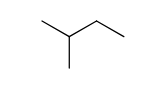
\includegraphics{smile-9b18206269c0e5315168c818cada3508c4456958}\\
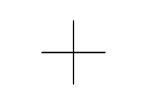
\includegraphics{smile-1b16cdc8f93c395f76114e6dea46fbed71b8157e}\\
(c) $\mathrm{C}_{5} \mathrm{H}_{11}$ can be represented as :\\
(i) $n$-Pentyl\\
(ii) Isopentyl (3-methylbutyl)\\
(iii) Active amyl ( 2 -methylbutyl)\\
(iv) Tertiary pentyl (1,1-dimethylpropyl)\\
(v) Neo pentyl (2,2-dimethylpropyl)\\
(vi) Active secondary amyl (1-methylbutyl)\\
(vii) Secondary amyl (1-ethylpropyl)\\
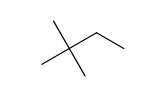
\includegraphics{smile-8274e4bb2805fc05d4ab72e237aa728afc1649c2}\\
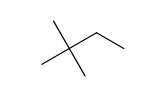
\includegraphics{smile-a11cf87c85f8adebb294eecf7acec3028fe902c2}\\
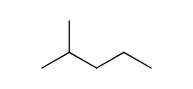
\includegraphics{smile-658c8c4f6597d53731c9ea130c204aea17736299}\\
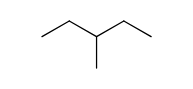
\includegraphics{smile-decea1135af0a11aae3824d452c96e15635d1f05}\\
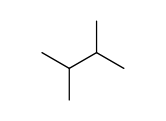
\includegraphics{smile-5e3b3a728e991a3498a7486f08739f4daa1825b0}\\
(1,2-dimethyl propyl)

\section*{Alkenyl group:}
$\mathrm{CH}_{2}=\mathrm{CH}-\operatorname{Vinyl}$ (ethenyl) ; $\mathrm{CH}_{2}=\mathrm{CH}-\mathrm{CH}_{2}-$ Allyl (2-Propenyl)\\
$\mathrm{CH}_{3}-\mathrm{CH}=\mathrm{CH}-\mathrm{Propenyl}$ (1-propenyl) $; \mathrm{CH}_{3}-\underset{\text { I }}{\mathrm{C}}=\mathrm{CH}_{2}$ Isopropenyl

\section*{Alkynyl group:}
$\mathrm{CH} \equiv \mathrm{C}-\quad$ Acetynyl (Ethynyl)\\
$\mathrm{CH} \equiv \mathrm{C}-\mathrm{CH}_{2}-\quad$ Propargyl (2-propynyl) \& $\mathrm{CH}_{3}-\mathrm{C} \equiv \mathrm{C}$ - Propynyl (1-propynyl)\\
Functional group : Organic compounds made up of only carbon and hydrogen are termed as hydrocarbons and they are parent organic compounds.\\
All other compounds are considered to have been derived from them by replacing one or more hydrogen by some other atom or group of atoms. These atoms or group are termed as functional group and they largely determine the chemical properties of the compound. The functional groups show their individual identity in their chemical reactions. Generally, compounds having same functional group show same chemical reactions. Some important functional groups are shown in the following table.

\begin{center}
\begin{tabular}{|l|l|l|}
\hline
Name of functional group & Formula of functional group & Example \\
\hline
 & I &  \\
Alkane & $-\mathrm{C}-$ & $\mathrm{CH}_{3}-\mathrm{CH}_{3}$ \\
 &  &  \\
Alkene & $\mathrm{C}=\mathrm{C}$ & $\mathrm{CH}_{2}=\mathrm{CH}_{2}$ \\
Alkyne & $-\mathrm{C} \equiv \mathrm{C}-$ & $\mathrm{CH}=\mathrm{CH}^{2}$ \\
Halide & -X & $\mathrm{CH}_{3}-\mathrm{CH}_{2} \mathrm{Cl}$ \\
Alcohol & -OH & $\mathrm{CH}_{3}-\mathrm{CH}_{2}-\mathrm{OH}$ \\
Thioalcohol & -SH & $\mathrm{CH}_{3}-\mathrm{CH}_{2}-\mathrm{SH}$ \\
\hline
\end{tabular}
\end{center}

\begin{center}
\begin{tabular}{|c|c|c|c|}
\hline
\begin{tabular}{l}
Ether \\
Aldehyde \\
\end{tabular} & \( \begin{aligned} & -\mathrm{O}- \\ & -\mathrm{CHO} \end{aligned} \) &  & \( \mathrm{CH}_{3}-\mathrm{CHO} \quad \mathrm{CH}_{3}-\mathrm{O}-\mathrm{C} \) \\
\hline
Ketone & 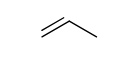
\includegraphics{smile-30c955f0f12d1809179842f9c1e897eb658d8c84} &  &  \\
\hline
Carboxylic acid & - COOH &  & $\mathrm{CH}_{3}-\mathrm{COOH}$ \\
\hline
Ester & - COOR &  & $\mathrm{CH}_{3} \mathrm{COOCl}$ \\
\hline
Acid anhydride & 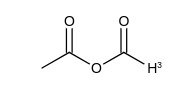
\includegraphics{smile-d03bc119c8d78f0a41c1c91499af2d35ff08db5c} &  & 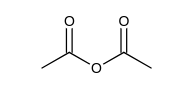
\includegraphics{smile-d836e7836f0c183d8731c0e93f0d34039e14fb68} \\
\hline
Acid amide Cyanide & \( -\mathrm{CONH}_{2} \) &  & \( \mathrm{CH}_{3} \mathrm{CN}^{\mathrm{CH}_{3} \mathrm{CONH}} \) \\
\hline
Amine & $-\mathrm{NH}_{2}$ &  & $\mathrm{CH}_{3} \mathrm{NH}_{2}$ \\
\hline
Nitro & $-\mathrm{NO}_{2}$ &  & $\mathrm{CH}_{3} \mathrm{NO}_{2}$ \\
\hline
Sulphonic acid & $-\mathrm{SO}_{3} \mathrm{H}$ &  & $\mathrm{CH}_{3} \mathrm{CH}_{2} \mathrm{SO}_{3} \mathrm{H}$ \\
\hline
Isocyanide & - NC &  & $\mathrm{CH}_{3} \mathrm{NC}$ \\
\hline
\end{tabular}
\end{center}

\section*{HOMOLOGOUS SERIES:}
When structurally similar organic compounds are arranged in the order of increasing molecular weight, then the series of compounds so obtained is called a homologous series. The members of such a series are known as homologous of one another and this property is called homology.\\
Characteristics of Homologous Series :

\begin{enumerate}
  \item All the members of a homologous series can be represented by only one general formula.
  \item The members of a homologous series differ in their molecular weight by 14 or its multiple.
  \item The members of a homologous series differ in their molecular formulae by $\mathrm{CH}_{2}$ or its multiple.
  \item The members of a homologous series can be synthesised by some general methods of preparation.
  \item Physical properties of the members of a homologous series normally exhibit a regular gradual change with increase in molecular weight.
  \item The members of a homologous series normally exhibit similar chemical properties (reactions).
  \item Homologues cannot be isomers due to difference in their molecular formulae. Therefore, two or more than two isomers can never be included in the same homologous series.
\end{enumerate}

Ex.: Series\\
Alkane\\
Alkene\\
Alkyne\\
Alkanol\\
Alkanal\\
Alkanoic acid -

\section*{Member}
$\mathrm{CH}_{4}, \mathrm{C}_{2} \mathrm{H}_{6}$ etc.\\
$\mathrm{C}_{2} \mathrm{H}_{4}, \mathrm{C}_{3} \mathrm{H}_{6}$ etc.\\
$\mathrm{C}_{2} \mathrm{H}_{2}, \mathrm{C}_{3} \mathrm{H}_{4}$ etc.\\
$\mathrm{CH}_{3} \mathrm{OH}, \mathrm{C}_{2} \mathrm{H}_{5} \mathrm{OH}$ etc.\\
$\mathrm{HCHO}, \mathrm{CH}_{3} \mathrm{CHO}$ etc.\\
$\mathrm{HCOOH}, \mathrm{CH}_{3} \mathrm{COOH}$ etc. $\mathrm{C}_{n} \mathrm{H}_{2 n} \mathrm{O}_{2}$

Alkylamines ( $1^{\circ}$ or primary amines), Dialkylamines ( $2^{\circ}$ or secondary amines) and Trialkylamines ( $3^{\circ}$ or tertiary amines) constitute different homologous series.

\section*{NOMENCEATURE:}
Mainly three systems are adopted for naming of organic compounds\\
(i) Common names or Trivial system\\
(ii) Derived system\\
(iii) IUPAC system

Initially organic compounds are named on the basis of source from which they were obtained.

\begin{center}
\begin{tabular}{|c|c|c|c|}
\hline
S. No. & Organic Compound & Trivial Name & Source \\
\hline
1. & $\mathrm{CH}_{3} \mathrm{OH}$ & Wood spirit or Methyl spirit & Obtained by destructive distillation of wood. \\
\hline
2. & $\mathrm{C}_{2} \mathrm{H}_{5} \mathrm{OH}$ & Grain Alcohol & Obtained by fermentation of barley \\
\hline
3. & $\mathrm{NH}_{2} \mathrm{CONH}_{2}$ & Urea & Obtained from urine \\
\hline
4. & $\mathrm{CH}_{4}$ & Marsh gas (fire damp) & It was produced in marsh places. \\
\hline
5. & $\mathrm{CH}_{3} \mathrm{COOH}$ & Vinegar & Obtained from acetum i.e. vinegar \\
\hline
6. & \( \underset{\mathrm{I}}{\mathrm{COOH}} \) & Oxalic acid & Obtained from oxalis plant \\
\hline
 & COOH &  &  \\
\hline
7. & HCOOH & Formic acid & \begin{tabular}{l}
Obtained from formicus \\[0pt]
[Red ant] \\
\end{tabular} \\
\hline
8. & 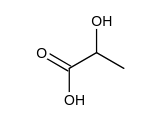
\includegraphics{smile-b196aa8ae386545320adf8e264f5b35909a871f7} & Lactic acid & Lactum $=$ milk \\
\hline
9. & $\mathrm{CH}_{2} \mathrm{COOH}$ & Malic acid & Apple(Malum) \\
\hline
 & $\mathrm{CH}(\mathrm{OH}) \mathrm{COOH}$ &  &  \\
\hline
10. & $\mathrm{CH}_{3} \mathrm{CH}_{2} \mathrm{CH}_{2} \mathrm{COOH}$ & Butyric acid & Obtained from butter \\
\hline
\end{tabular}
\end{center}

Some typical compounds in which common and trivial names also differ\\
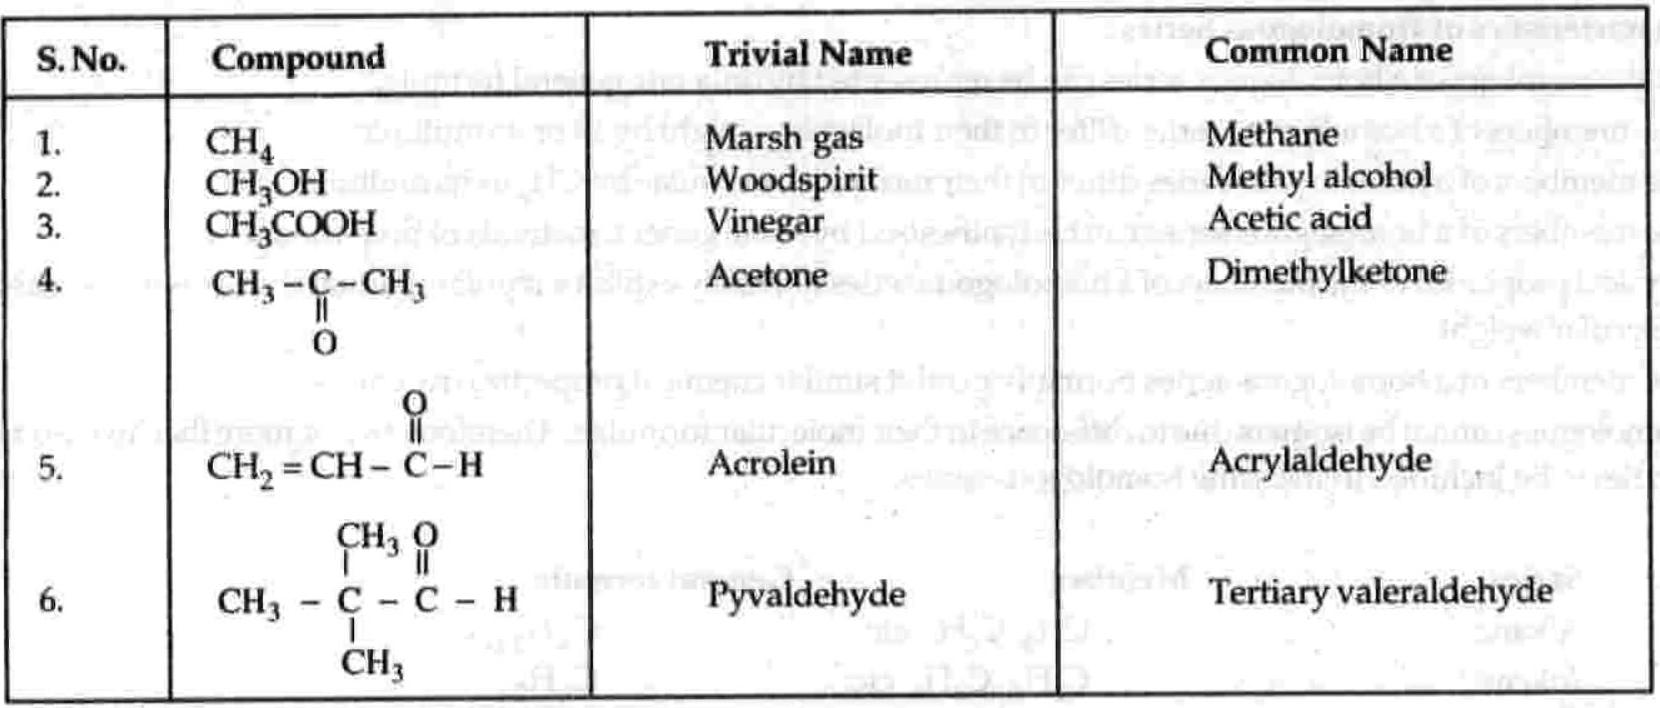
\includegraphics[max width=\textwidth, center]{2025_01_28_8470952b98110cec3aabg-012}\\
(Common Names; $\mathbf{R}$ is termed as alkyl -):

\begin{center}
\begin{tabular}{|l|l|l|}
\hline
S.No. & Compound & Name \\
\hline
1. & $\mathrm{R}-\mathrm{X}$ & Alkyl halide \\
2. & $\mathrm{R}-\mathrm{OH}$ & Alkyl alcohol \\
3. & $\mathrm{R}-\mathrm{SH}$ & Alkyl thioalcohol \\
4. & $\mathrm{R}-\mathrm{NH}_{2}$ & Alkylamine \\
5. & $\mathrm{R}-\mathrm{O}-\mathrm{R}$ & Dialkyl ether \\
6. & $\mathrm{R}-\mathrm{S}-\mathrm{R}$ & Dialkyl thioether \\
7. & $\mathrm{R}-\mathrm{C}-\mathrm{R}$ & Dialkylketone \\
 & O &  \\
8. & $\mathrm{O}-\mathrm{NH}-\mathrm{R}$ & Dialkyl amine \\
\hline
\end{tabular}
\end{center}

\begin{center}
\begin{tabular}{|l|c|c|}
\hline
9. & $\mathrm{R}-\mathrm{N}-\mathrm{R}$ & Trialkyl amine \\
10. & R &  \\
11. & $\mathrm{R}-\mathrm{O}-\mathrm{R}^{\prime}$ & Alkyl alkyl' ether \\
 & $\mathrm{R}-\mathrm{C}-\mathrm{R}^{\prime}$ & Il \\
12. & O & Alkyl alkyl' ketone \\
13. & $\mathrm{R}-\mathrm{S}-\mathrm{R}^{\prime}$ &  \\
$\mathrm{R}-\mathrm{NH}-\mathrm{R}^{\prime}$ & Alkyl alkyl' thioether &  \\
14. & $\mathrm{R}-\mathrm{N}-\mathrm{R}^{\prime}$ & Alkyl alkyl' amine \\
 & $\mathrm{R}^{\prime \prime}$ & Alkyl alkyl' alkyl" amine \\
\end{tabular}
\end{center}

Position of double bond: In an unsaturated hydrocarbon if the position of double is on $1^{\text {st }}$ or last carbon then its prefix will be $\alpha$ (alpha), if it is on $2^{\text {nd }}$ carbon it is termed as $\beta$ (beta) and then $\gamma$ (gamma), $\delta$ (delta) and so on.\\
Ex. $\mathrm{H}_{2} \mathrm{C}=\mathrm{CH}-\mathrm{CH}_{2}-\mathrm{CH}_{3}$ or $\mathrm{H}_{3} \mathrm{C}-\mathrm{CH}_{2}-\mathrm{CH}=\mathrm{CH}_{2} \quad \alpha$-butylene\\
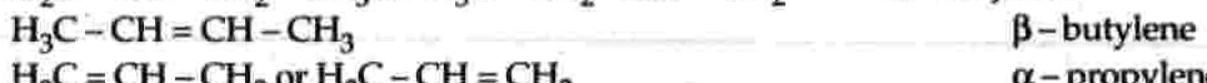
\includegraphics[max width=\textwidth, center]{2025_01_28_8470952b98110cec3aabg-013(2)}\\
$\mathrm{H}_{2} \mathrm{C}=\mathrm{CH}-\mathrm{CH}_{3}$ or $\mathrm{H}_{3} \mathrm{C}-\mathrm{CH}=\mathrm{CH}_{2} \quad \alpha$-propylene\\
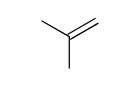
\includegraphics{smile-bf8dfaeffee0d4292c2a0e033e99c369f87ffa98}

Isobutylene\\
\includegraphics{smile-4cd05599b48f91a9771f2bb9da55cdafdba33a2c}\\
$\gamma$-hexylene\\
$\delta$-octylene

\section*{Common naming of dihydroxy compounds :}
(a) When two - OH groups are attached to adjacent carbons they are termed as alkylene glycol.

Ex.\\
\includegraphics{smile-23106b9615eab6e0b06ce595e3dffea3e5e5cd10}\\
\includegraphics{smile-9ce4db110eee62cad2703ce80d5401f3f965d2e5}\\
\&\\
\includegraphics{smile-ef2f748282dc31c51d4d6784a52b9beddcb6f328}

Active amylene glycol\\
(b) When two- OH groups are attached at the twoends of a carbon chain, these compounds are named as polymethylene glycols. Poly $\rightarrow$ Number of $\mathrm{CH}_{2}$ groups.

Ex.\\
\includegraphics{smile-882817cae275d70c1ccdfdd38312cb540a8c4564}

Tetramethylene glycol\\
\includegraphics[max width=\textwidth, center]{2025_01_28_8470952b98110cec3aabg-013}

Exception:\\
$\begin{array}{ll}\mathrm{CH}_{2}-\mathrm{OH} & \text { dimethylene glycol (wrong) } \\ \mathrm{CH}_{2}-\mathrm{OH} & \text { ethylene glycol }\end{array}$

\section*{Common-naming of dihalides :}
(a) When two same halogen atoms are attached to the same carbon, such compounds are called gemdihalides.\\
(b) Common names of such compounds are alkylidene halides.

Ex.\\
\includegraphics[max width=\textwidth, center]{2025_01_28_8470952b98110cec3aabg-013(1)}

Isobutylidene iodide\\
\includegraphics[max width=\textwidth, center]{2025_01_28_8470952b98110cec3aabg-013(3)}\\
(c) When two same halogen atoms are attached to adjacent carbons, these are called as vicinal dihalides common names of such compounds are alkylene halides.\\
Ex.\\
\includegraphics{smile-a061a72aef109c86ac9fd28102ddc28b6de2d43f}\\
\includegraphics{smile-98f924914bb8b3d12738c4de9a6d5aaddcc33316}\\
\includegraphics{smile-f5ed8561f741b1683d2b72351e633a590d7ed07b}

Propylene lodide Isobutylene chloride Ethylene chloride\\
(d) When two same halogen atoms are attached at the two ends of a carbon chain, its common name will be polymethylene halide. 'poly' word indicates the number of $-\mathrm{CH}_{2}$ - groups.

\begin{center}
\begin{tabular}{llllll}
$-\mathrm{CH}_{2}-2$ & 3 & 4 & 5 & 6 &  \\
Poly & di & tri & tetra & penta & hexa \\
\end{tabular}
\end{center}

Ex.\\
\includegraphics{smile-5af8ad478ed7834f43e8a1fc891449c2e421ec03}\\
\includegraphics{smile-523c328527d901e9cf6ad3418776e0f172d8cd6a}

Exception: $\underset{\mathrm{CH}_{2}-\mathrm{X}}{\mathrm{CH}_{2}-\mathrm{X}} \quad$ dimethylene halide (wrong)

\section*{Examplened 1:}
Write down the structure of following organic compounds -

\begin{enumerate}
  \item Isopropylidene bromide
  \item Active amylene iodide
  \item Isobutylene
  \item Trimethylene glycol
\end{enumerate}

\section*{3. Isobutylene glycol}
Sol. 1.\\
\includegraphics{smile-91e9bd7c4f6752a2a5abe8b37db85259d134257b}\\
2.\\
\includegraphics{smile-e64c3b33281c7596287d3427ac656ae603e7093c}\\
3.\\
\includegraphics{smile-bdf1ef205f526ad49ce693854ec9ecd664787963}\\
4.\\
\includegraphics{smile-db263b8692a384a325cc5560fce99e05fe660348}\\
5. $\underset{\substack{\mathrm{CH}_{2} \\ \mathrm{OH}}}{\mathrm{OH}_{2}}-\mathrm{CH}_{2}-\mathrm{CH}_{2}$

Common name of the functional groups having carbon :\\
\includegraphics[max width=\textwidth, center]{2025_01_28_8470952b98110cec3aabg-014(1)}\\
\includegraphics[max width=\textwidth, center]{2025_01_28_8470952b98110cec3aabg-014}

Ex.\\
\includegraphics{smile-141f3f6df1755919faea12e8add1ce78b8cad1b0}\\
\includegraphics{smile-6294ab28269a31048369c56354f06664a68bafa1}\\
\includegraphics{smile-4a7c98a6413dbf2b0348cbe52b2f9ca7d272cca3}\\
\includegraphics{smile-05b74c8919d24c966d50040901dc681614b2f864}\\
\includegraphics{smile-710cde5de6d3243827a3e669cdc3f10ca6853844}

Formaldehyde Acetic Acid Propionyl chloride Isobutyramide Acetaldehyde\\
Nomenclature of ester : $-\stackrel{\text { II }}{\mathrm{C}}-\mathrm{O}-\mathrm{R}$\\
The group which is attached to the oxygen is written as alkyl and the remaining structure is named according to previous discussions.

Ex.\\
\includegraphics[max width=\textwidth, center]{2025_01_28_8470952b98110cec3aabg-015(1)}\\
\includegraphics[max width=\textwidth, center]{2025_01_28_8470952b98110cec3aabg-015}\\
\includegraphics{smile-78fea33a78700013869cd81231b83881b1b67435}

Nomenclature of anhydride :\\
\includegraphics{smile-d0d278368cb4794c6be73815cd24cfdbad7c08fa}

Rule: Add the total number of carbon atoms and divide it by 2, the substract will give you the number of C -atom.

$$
\frac{\text { Total }}{2}=\text { Substract }=\text { Number of } C \text { atom. }
$$

\includegraphics{smile-2a7b904b28cee2ee2e6046b8c339e221fe101a71}

In\\
\includegraphics{smile-b69ba3cec049e8d14f4e0abbbf156d413213d14c}\\
\includegraphics{smile-5810584d113f023d2a8f5e9ff949540de0a587de}

Acetic propionic anhydride (right). Propionic acetic anhydride (wrong)\\
Divide it in two parts as above and name it by suffixing 'ic anhydride' (alphabatically)

Ex.\\


Butyric propionic anhydride

Ex.\\
\includegraphics{smile-0212c550376bcebaa112c9490b523da9e0d69fa7}\\
\includegraphics{smile-9f12d69d805c227bc2d0b2ef5c272d1d4e0d2b96}

\section*{DERIVED SYSTEM:}
According to this system name to any compound is given according to the parent name of the homologous series. This system is reserved for the following nine homologous series.\\
\includegraphics[max width=\textwidth, center]{2025_01_28_8470952b98110cec3aabg-016}\\
Ex.\\
\includegraphics{smile-d931cbc443b2ba338bf41680aec6f71a27c670dc}\\
\includegraphics{smile-a0c0ebc6fa6bc0fdc48afac51c586bd7eb1cb9aa}\\
\includegraphics{smile-3e3353bb5c6dd976261b284da8b4c11a9493391c}\\
\includegraphics{smile-a086b2f184130369efaa00fa73d89b817c87d601}\\
\includegraphics{smile-e76e4f7273362deccee30f5587ef3755e9b9a344}

Tetramethyl-methane Dimethylacetylene Trimethyl-carbinol Trimethyl-acetalddehyde Trimethyl-aceticacid

\section*{Types of ethylene : (Symmetrical and Unsymmetrical)}
Note :-Symmetrical and Unsymmetrical terms are used only when two alkyl groups are given.\\
(a) Symmetrical : Of the two alkyl groups one group is attached to one carbon of ethylene and the other to the next carbon.\\
(b) Unsymmetrical : When both the alkyl groups are attached on the same carbon.\\
Ex.\\
\includegraphics{smile-104aaca7d5934eb3eb8139ccb31fa9d3cb43c83d}\\
\includegraphics{smile-45e0a75d0d6830aa857f685d13b1670a238876fb}\\
\includegraphics{smile-87cccd936b3c81cca6bed97ad024494ea6a2cc85}

Symmetrical dimethylethylene\\
Unsymmetrical dimethylethylene\\
\includegraphics{smile-805c5486bbfb7e76d897bb7f7e321b6571bb85b0}\\
\includegraphics{smile-f2f0dfedd787696375209135885445722830bbff}

Tetramethylethylene\\
$\mathrm{CH}_{3}-\mathrm{C} \equiv \mathrm{C}-\mathrm{CH}_{3}$

Dimethylacetylene

\section*{IUPAC SYSTEM:}
IUPAC system of nomenclature of aliphatic compounds\\
According to IUPAC system, the name of an organic compound consists of three parts\\
(i) Word root\\
(ii) Suffix\\
(iii) Prefix\\
(i) Word root: Word root denotes the number of carbon atoms present in the principal chain which is the longest possible chain of carbon atoms. According to chain length, word root name up to $\mathrm{C}_{12}$ are given below.

\begin{center}
\begin{tabular}{|l|l|l|l|}
\hline
Chain Length & Word Root & Chain Length & Word Root \\
\hline
$\mathrm{C}_{1}$ & Meth & $\mathrm{C}_{7}$ & Hept (a) \\
$\mathrm{C}_{2}$ & Eth & $\mathrm{C}_{8}$ & $\operatorname{Oct(a)}$ \\
$\mathrm{C}_{3}$ & Prop & $\mathrm{C}_{9}$ & Non(a) \\
$\mathrm{C}_{4}$ & But(a) & $\mathrm{C}_{10}$ & Dec(a) \\
$\mathrm{C}_{5}$ & Pent(a) & $\mathrm{C}_{11}$ & Undec (a) \\
$\mathrm{C}_{6}$ & Hex(a) & $\mathrm{C}_{12}$ & Dodec(a) \\
\hline
\end{tabular}
\end{center}

Extra ' $a$ ' given in parenthesis is used only if the primary suffix to be added to the word root starts with a consonant. Consonant-di, tri, tetra etc are not started with vowel, then extra ' $a$ ' has been added to the word root.\\
(ii) Suffix - Suffixes are of two types. Primary and secondary suffixes.\\
(a) Primary suffix - A primary suffix indicates the type of linkage in the carbon chain. If the carbon atoms are linked by single covalent bonds, the primary suffix is 'ane'. If these are linked by double and triple bonds, the primary suffixes 'ene' and 'yne' are respectively used to represent them. Thus, ane: primary suffix for $\mathrm{C}-\mathrm{C}$ bond ene: primary suffix for $\mathrm{C}=\mathrm{C}$ bond yne: primary suffix for $\mathrm{C} \equiv \mathrm{C}$ bond\\
If the parent chain of carbon atoms contains more than one double or triple bonds, numerical prefixes like di (for two), tri (for three) tetra (for four) etc. are added to primary suffix.\\
Example -

\begin{center}
\begin{tabular}{llll}
Hydrocarbon & Word root & Primary suffix & IUPAC name \\
$\mathrm{CH}_{3}-\mathrm{CH}_{2}-\mathrm{CH}_{2}-\mathrm{CH}_{3}$ & But & ane & Butane \\
$\mathrm{CH}_{2}=\mathrm{CH}-\mathrm{CH}=\mathrm{CH}_{2}$ & Buta$^{*}$ & diene & Butadiene \\
$\mathrm{CH}_{3}-\mathrm{C} \equiv \mathrm{CH}$ & Prop & yne & Propyne \\
\end{tabular}
\end{center}

(b) Secondary suffix: A secondary suffix is used to represent the functional group if present in organic molecule and is attached to the primary suffix while writing its IUPAC name. Secondary suffixes of some of the functional groups are:

\begin{center}
\begin{tabular}{|c|c|c|c|}
\hline
Functional group & Symbol & Suffix & Prefix \\
\hline
Sulphonic Carboxylic & \( \begin{aligned} & -\mathrm{SO}_{3} \mathrm{H} \\ & -\mathrm{COOH} \end{aligned} \) & sulponic acid -oic acid & sulpho carboxy \\
\hline
Ester & \includegraphics{smile-5467524ba8397d8faed6bc177bc3e4ac00cbdbb5} & Alkyl-alkanoate alky alkoxy carbonyl & 1 carboxylate or \\
\hline
Acid halide & \includegraphics{smile-5e6c2f49914ffaab8db17921bd00ee39edd216d5} & - oylhalide & Halo formyl \\
\hline
Acid amide & \includegraphics{smile-b36163a7c493d586d3997336e14557728123fd69} & amide & carbamoyl \\
\hline
Aldehyde & \( \|_{-\mathrm{C}-\mathrm{H}}^{0} \) & -al & Formyl/ Aldo \\
\hline
cyanide isocyanide & \( \begin{aligned} & -\mathrm{C} \equiv \mathrm{~N} \\ & \mathrm{~N} \equiv \mathrm{C} \end{aligned} \) & \begin{tabular}{l}
-nitrile \\
-isocyanide \\
\end{tabular} & Cyano Isocyano \\
\hline
isocyamide ketone & $\rightarrow \mathrm{N}=\mathrm{C}>\mathrm{C}=0$ & bat -one & keto, oxo \\
\hline
hydroxy &  & -ol & hydroxy \\
\hline
\end{tabular}
\end{center}

CHEMISTRY

\begin{center}
\begin{tabular}{|l|c|l|l|}
\hline
Thioalcohol & -SH & \begin{tabular}{l}
Thiol \\
Amine \\
\end{tabular} & \begin{tabular}{l}
-Amine \\
amino \\
\end{tabular} \\
Secondary amine & $-\mathrm{NH}_{2}$ & N -Alkylamine & N -alkylamine \\
Tertiaryamine & -N &  &  \\
 &  &  &  \\
Nitro & -N & N -alkyl- N -alkylamine & N -alkyl- N -alkylamine \\
\hline
\end{tabular}
\end{center}

Groups given below does not have any suffix

Ither\\
Epoxide\\
-OR\\
Azo $\quad-\mathrm{N}=\mathrm{N}-$\\
Nitroso $\quad-\mathrm{NO}$\\
Halogen\\
$-\mathrm{X}(\mathrm{F}, \mathrm{Cl}, \mathrm{Br}, \mathrm{I})$\\
\includegraphics[max width=\textwidth, center]{2025_01_28_8470952b98110cec3aabg-018}

While adding a secondary suffix to the primary suffix, the terminal ' $e$ ' of the primary suffix (ane, ene, or yne) is dropped if the secondary suffix begins with ' $a^{\prime}$ ', $i^{\prime}$ ' $\mathrm{o}^{\prime}$ ' $u$ ' or ' $\mathbf{y}$ '. In case, it begins with consonant, then the terminal ' $e^{\prime}$ of the primary suffix is retained.\\
Ex.\\
Organic compounds\\
$\mathrm{CH}_{3} \mathrm{CH}_{2} \mathrm{OH}$\\
$\mathrm{CH}_{3} \mathrm{CH}_{2} \mathrm{CHO}$\\
$\mathrm{CH}_{3} \mathrm{CH}_{2} \mathrm{CH}_{2} \mathrm{NH}_{2}$\\
$\mathrm{CH}_{3} \mathrm{CH}_{2} \mathrm{CN}$

Word root Primary suffix

\begin{center}
\begin{tabular}{lll}
eth & an(e) & ol \\
prop & ane(e) & al \\
prop & ane(e) & amine \\
prop & ane & nitrile \\
\end{tabular}
\end{center}

\section*{Secondary suffix IUPAC name}
\begin{center}
\begin{tabular}{ll}
of & Ethanol \\
al & Propanal \\
amine & Propanamine \\
nitrile & Propanenitrile \\
\end{tabular}
\end{center}

Ethanol Propanal Propanenitrile\\
(iii) Prefix: Prefix is a part of IUPAC name which appears before the word root. Prefixes are of two types.\\
(a) Primary prefix - A primary prefix "cyclo" is used in order to differentiate a cyclic compound from an acyclic compound.\\
Forexample\\
\includegraphics{smile-adc1043f9808a213f19713fd996d43157af628f7}\\
\includegraphics{smile-7b20b37ab8915e7e5ca12c21028a04d40db61998}\\
\includegraphics{smile-955b5b1baa4d3faaa2d6370b3bf55a03172e96d4} Cyclopropane\\
\includegraphics{smile-29af6c8e54407dab63d8ce9c28f1a2aecd27c962}\\
\includegraphics{smile-7a33fdfe40081e4a35b1902dc24f1973a2d2b4fd}

Propane and butane are the IUPAC names of acyclic compounds while cyclopropane and cyclobutane are for cyclic compounds.\\
(b) Secondary prefix - In the IUPAC system of nomenclature, certain characteristic groups are not considered as or secondary suffixes. These are regarded as substituents and are denoted by secondary prefixes. The secondary prefixes of a few substituents are given-\\
Substituent group\\
$-\mathbf{F}$\\
-Cl\\
-Br\\
-1\\
-NO

\begin{center}
\begin{tabular}{l}
Secondary prefix \\
Fluoro \\
Chloro \\
\hline
Bromo \\
lodo \\
\hline
Nitroso \\
\hline
\end{tabular}
\end{center}

Secondary prefix\\
Nitro\\
Methyl\\
Ethyl Methoxy Ethoxy

Besides these, some other functional groups are also treated as substituents in case of poly functional organic compounds. These are listed as\\
\includegraphics[max width=\textwidth, center]{2025_01_28_8470952b98110cec3aabg-019(2)}

General rules for naming long chain aliphatic compounds : Many organic compounds contain long chains which may include substituents, multiple bonds and functional groups. The IUPAC names of such compounds are based on certain general rules.\\
Rules for IUPAC nomenclature of straight and branched chain alkanes : In writing the IUPAC name of an aliphatic compounds the following sequence is used. Secondary prefix + primary prefix + word root + primary suffix + secondary suffix

\begin{enumerate}
  \item Longest chain rule-Select the longest continuous chain of carbon atoms in a given molecule of alkane which need not be straight. It is known as parent chain or principal chain.\\
\includegraphics[max width=\textwidth, center]{2025_01_28_8470952b98110cec3aabg-019(1)}
\end{enumerate}

Parent chain has six carbon atoms and $\mathrm{CH}_{3}$ group represents the substituent\\
If two chains of equal lengths are possible, then the one with more number of side chains (or substituents) represents the parent chain. For example,\\
\includegraphics{smile-4d19bb2ab14985fbb098e3fea672371ea719e01d}\\
(Parent chsin of sic carbon atom has ane cubstithent) Wron?\\
\includegraphics[max width=\textwidth, center]{2025_01_28_8470952b98110cec3aabg-019}\\
(Pafent cliain of sic carbon atoms has two substimentst Kight\\
2. Lowest number rule - For molecules with only one substituent, number the carbon atoms as $1,2,3,4 \ldots \ldots$. etc. in the parent chain starting from one end in sucha way that the carbon atom carrying the substituent gets the lowest number.\\
\includegraphics{smile-21da64147963a1ef64e5cc22eb8aa1ad496bc50f}

The numbering of parent chain is correct because\\
$\mathrm{CH}_{3}$ group is attached to $\mathrm{C}-3$ atom\\
\includegraphics{smile-7778c06c05bb38204887bf2c2105cee6d313d307}

The numbering of parent chain is incorrect

The number which indicates the position of the substituent (or side chain) in the parent chain is called its position number or locant. The name of the substituents is separated from its locant by hyphen $(-)$ and the final name of the alkane is always written as one word i.e. 3-methylheptane. In case, same alkyl group occurs more than once at different positions in the parent chain, the positional number of each alkyl group is separated by commas and suitable prefixes like di (for two), tri (for three) tetra (for four) etc. are attached to the name of the alkyl groups.\\
3. Lowest set of locants rule - In case, there are two or more substituents, then the parent or principal chain is numbered from the end which gives the lowest set of locants. This rule (IUPAC 1993) replaces the lowest sum rule used earlier. When two or more substituents are present in a molecule, then the end of the parent chain which gives the lowest term at the first point of difference in the set of locants is considered for numbering the carbon atoms in the parent chain.

Ex.\\
\includegraphics{smile-fd958f065ee02fd41d29a18b67f07e156a81c4d5}

Set of locants : 2, 4,9 locants Correct\\
\includegraphics{smile-0709ae9e8b85bb11bf01315c60d3b9ec5f5ced40}

Set of locants : $2,7,9$ locants Wrong\\
Alphabetical order for the side chain (or substituents) - When two or more different alkyl groups (side chains or substituents) are present on the parent chain. Such groups prefixed by their locants (or positional numbers) are arranged in alphabetical order irrespective of their positional number, before the name of the parent alkane. For example,\\
\includegraphics[max width=\textwidth, center]{2025_01_28_8470952b98110cec3aabg-020}

It may be remembered that the prefixes di, tri, tetra are not considered in case the same alkyl group occurs more than one on the parent chain at different positions while arranging them in an alphabetical order. For example,\\
\includegraphics{smile-95312794c16f67a554f0bd87e70d94ddeb4d7c02}

3-Ethyl-2.3-dimethylpentane\\
Naming the different substituents at equivalent positions - If two different substituents are present at equivalent positions from the two ends in the parent chain, then the numbering of the chain is done in such a way that the substituent which comes first in the alphabetical order gets the lower number. For example\\
\includegraphics{smile-9afdbe6eeebc88ad856010be37f98bf62bdfe04c}

3-Ethyl-4-methylhexane hamsend\\
4. Naming the complex substituents or alkyl groups:\\
(a) An alkyl group is said to be complex in case one or more carbon atoms in it are further substituted i.e., it is a substituted substituent (or alkyl group). It is named as a substituted alkyl group by numbering from the carbon atom of this group attached to the parent chain as " 1 ". The name of the complex substituent is generally enclosed in brackets in order to avoid any confusion with either numbering the parent chain or naming the other substituents attached to the chain. For example:\\
\includegraphics{smile-ed1c8218c3461fd684b7c4b14cc1946c88bd727c}

4-(1,1-dimethyiethyl) heptane\\
(b) It may be noted that while deciding the alphabetical order of the various substituents, the name of the complex substituent is considered to begin with the first letter of its complete name. For example-\\
\includegraphics[max width=\textwidth, center]{2025_01_28_8470952b98110cec3aabg-021}\\
(c) When the names of the complex substituents are composed of identical words, the priority is decided by comparing the locant at the first cited point within the complex substituents. This means that the complex substituent gets lower priority which has the lowest locant. For example\\
\includegraphics[max width=\textwidth, center]{2025_01_28_8470952b98110cec3aabg-021(2)}

5-(1-methylpropyl)-6-(2-methylpropyl) decane\\
In this case, 1-methylpropyl gets priority over 2-methylpropyl since the locant for the methyl substituent in the first case is less.

\section*{NOTE}
(a) Initially w rite the number of that carbon on which the side chain is attached, then write it in alkyl group.\\
(b) If there are more than one side chains (same) initially write the numbers altogether using symbol (). in between them, after last number use the symbol hyphen $(-)$. Write the numbers in increasing order.

Ex.\\
\includegraphics{smile-242bf84f71365b6c75a4652604fd62e4201b762e}

2,3,4-trimethylpentane\\
(c) IUPAC name is written according to english alphabates (strictly).\\
\includegraphics[max width=\textwidth, center]{2025_01_28_8470952b98110cec3aabg-021(1)}

\section*{2-methyl-4-isopropyl-5-ethylheptane (wrong) \\
 5-ethyl-4-isopropyl-2-methylheptane (right)}
(d) Capital word is used for first substituent.

Ex.\\
\includegraphics{smile-49043efe505c91c8a6969f986bf7db810c014bcd}

3-Amino-4-ethyl-2-methylhexane (more correct)

\section*{Rule in IUPAC nomenclature of unsaturated hydrocarbons (alkenes and alkynes)}
In writing the IUPAC name of a particular member of the alkene or alkyne family, the primary suffix, 'ane' of corresponding alkane is replaced by the sulfix 'ene' or 'yne' respectively.

\begin{enumerate}
  \item The parent chain must include the multiple bond regardless of the fact whether it is longest continuous chain or not. For example,\\
\includegraphics{smile-af8c3e14c262b50e05b2da39caf69281e0b2f9b3}
  \item The numbering of the parent chain must be done in such a way that the first $C$-atom involved in the multiple bond gets the lowest number. According to the latest IUPAC convention, the locants for the multiple bonds (double or triple bonds) are placed immediately before the primary suffixes (ene or yne) which they represent. The earlier practice was to place the locant either before the word root (e.g., 2-butene) or after the name of the primary suffix (e.g., butene-2) but it is not regarded as proper. For example,\\
\includegraphics{smile-eaa462b167d5953ffbaa06ce124c24f34c8ddeb3} But-2-enc
  \item If the selected principal or parent chain contains two (or three) double or triple bonds, then the primary suffix-diyne (or triene) or -diene (or triyne) are used to represent these. In all these cases, terminal ' $a$ ' is also added to the word root. For example,
  \item If the parent chain includes both double and triple bonds, then the following points must be kept in mind.\\
(a) the unsaturated compound is always named as a derivative of alkyne i.e., primary suffix 'ene' always comes before 'yne'. In all such cases, the terminal ' $e$ ' of 'ene' is dropped if it is followed by the suffix starting with a, i, o, u or y. For example,
\end{enumerate}

$$
\begin{gathered}
\mathrm{CH}_{-}-\mathrm{CH}=\mathrm{CH}-\mathrm{C}^{2}=\mathrm{CH}=\mathrm{CH}-3 \text {-en- } 4 \text {-yne }
\end{gathered}
$$

(b) In case, the numbering from two different ends gives two different sets of locants, then the lower set of locants is preferred. For example,

$$
\stackrel{6}{\mathrm{C}} \mathrm{H}_{3}-\stackrel{5}{\mathrm{C}} \equiv \stackrel{+}{\mathrm{C}}-\stackrel{\mathrm{C}}{\mathrm{C}} \mathrm{H}_{2}-\stackrel{2}{\mathrm{C}} \equiv \stackrel{1}{\mathrm{C}} \mathrm{H}
$$

Hexa-1, 4 -diyne and nor hexa-2, 5-diyne\\
5. If the unsaturated hydrocarbon contains a side chain (or substituent) along with the multiple bonds, then the numbering of the parent or principal chain is done in such a way that the multiple bond gets the lowest set of locants. However, if the numbering from both ends gives the same set of locants to the multiple bonds, then the locant for the substituent must be minimum. For example,

$$
\begin{gathered}
\mathrm{CH}_{3} \\
\stackrel{+}{\mathrm{C}} \mathrm{H}_{2}=\stackrel{+}{\mathrm{C}} \mathrm{H}-\mathrm{C}_{\mathrm{C}}^{\mathrm{C}} \mathrm{H} \\
\text { 2-Methylbuta-L 3-diene } \\
\text { (Minimum locant for the } \mathrm{CH} \\
3
\end{gathered}
$$

$1 \quad 2 \stackrel{\mathrm{CH}_{3}}{13} 4_{4}$\\
$\mathrm{HC} \equiv \mathrm{C}-\mathrm{CH}-\mathrm{C} \equiv \mathrm{CH}$\\
3-Methylpenta-1,4-diyne

In some cases, more than two double bonds are present in the hydrocarbon and it is not possible to include all of them in the parent chain. In such cases, the following prefixes are used for the double bonded groups not involved in the chain.\\
$\mathrm{CH}_{2}=$\\
$\mathrm{CH}_{3}-\mathrm{CH}=$\\
$\mathrm{CH}_{2}=\mathrm{CH}-$\\
(Vinyl or ethenyl)\\
$\mathrm{CH}_{2}=\mathrm{CH}-\mathrm{CH}_{2}-$\\
(Allyl)

Nomenclature of monofunctional compounds : Compounds having one functional group are called monofunctional compounds. The various rules are:

\begin{enumerate}
  \item That longest chain is selected which contains functional group, even if other chain contains more number of carbon atoms.\\
If the functional group contains a carbon atom, that atom is also counted as a part of the chain.\\

  \item When more than one same functional groups are present, the carbon chain which contains maximum number of functional group is selected.\\
\includegraphics[max width=\textwidth, center]{2025_01_28_8470952b98110cec3aabg-023}
  \item When the functional g. oup does not have carbon atom then the carbon atom to which the functional group is attached should be included in the main chain.\\
\includegraphics{smile-0109eddd72f35dbda6283f35735f1142c3dea5f7}
  \item The selected carbon chain is numbered from that end to which the functional group is nearer.\\
\includegraphics{smile-d36b8deb34db6bcbdd0c78430fd5279cf93fd845}
  \item If the functional group is at the same distance from both the ends, then numbering is done from the end in which the substituent is nearer.\\
\includegraphics{smile-21723bae0da3cc8adf43f23f7e7a3fb65337480e}
  \item While writing name of the compound, the name of functional group along with its position is represented by suitable suffix and all the substituents are represented by suitable prefixes in their alphabetical order.\\
\includegraphics{smile-f5bd4a4178f23e18f1a93b52192ed274cd5fab7e}
\end{enumerate}

4-Methyl pentane-2-01\\
(a) -OH group is present as functional group so it is represented by suffix - ol\\
(b) Longest chain consist of five carbon atoms all having single bond between them so parent hydrocarbon is pentane.\\
(c) -OH group is present on carbon number 2 and substituent methyl group is present on carbon number 4 .

Above name is derived as :

\begin{center}
\begin{tabular}{cccc}
4-methyl & + & Pent & + \\
$\downarrow$ & $\downarrow$ & $\downarrow$ & ane \\
$\downarrow$ & + & $\downarrow$ &  \\
Prefix for & Parent & Saturated & Suffix for the \\
substituent & hydrocarbon & chain & functional group \\
\end{tabular}
\end{center}

\begin{enumerate}
  \setcounter{enumi}{6}
  \item The chain terminal functional group, viz., $-\mathrm{COOH},-\mathrm{CHO},-\mathrm{COOR},-\mathrm{CONH}_{2},-\mathrm{COCl},-\mathrm{C} \equiv \mathrm{N}$ etc., when present in the parent chain is always given number 1. Generally, the number 1 is omitted while writing the final names of the compound, For example,\\
\includegraphics[max width=\textwidth, center]{2025_01_28_8470952b98110cec3aabg-024}
  \item If an organic compound contains a functional group, multiple bond, and a side chain (substituent) then the following order of preference must be followed.
\end{enumerate}

Functional group $>$ Double bond $>$ Triple bond $>$ Side chain

Ex.\\
\includegraphics{smile-5e65898a1d176aba4463be9b0b3a398b8a96f67b}\\
\includegraphics{smile-f1d17dbb2e790df785553e444bf7343317af2e79}

2-ethyl-3-methyl butanoic acid\\
\includegraphics{smile-bea0be781518577d59f0b9d5412546a2061b1dea}

5-chloro-3-methyl hexane nitrile\\
Nomenclature of ether : The smaller alkyl group attached with oxygen is written as alkoxy and the longest chain of remaining carbons is selected.\\
Ex. Write the IUPAC name

\begin{enumerate}
  \item $\stackrel{3}{\mathrm{C}} \mathrm{H}_{3}-\stackrel{2}{\mathrm{C}} \mathrm{H}_{2}-\stackrel{\mathrm{C}}{\mathrm{C}} \mathrm{H}_{2}-\mathrm{O}-\mathrm{CH}_{3}$
\end{enumerate}

1-Methoxypropane\\
2. $\stackrel{3}{\mathrm{C}} \mathrm{H}_{3}-\stackrel{2}{\mathrm{C}} \mathrm{H} \mathrm{H}-\mathrm{O}-\mathrm{CH}_{3}$

2-Methoxypropane

Ex. Write the correct IUPAC name of the compound 2-ethoxybutane.\\
\includegraphics{smile-67395df032c2b8644bdac09223689e8686451b78}

Nomenclature of keto group : The carbon of a ketone is included in longest chain it never comes on first or last positions, whereas - CHO (Aldehyde group) comes at first and last position only.

Ex.\\
\includegraphics{smile-e946dc82b8a01ff938e96f55e9d4e2606ef33bf4}

3-Methyl-2-pentanone

IUPAC Momenclature for compounds containing more than one different functional groups (Polyfunctional compounds)\\
When an organic compound contains two or more different functional groups, then one of these is selected as principal functional group while the others are called secondary functional groups and are treated as substituents. The choice of the principal functional group is made on the basis of the of preferences.

\begin{center}
\begin{tabular}{|c|c|c|c|c|}
\hline
S. No. & Name & Formula & Functional group prefix & Suffix \\
\hline
1. & \multirow[t]{3}{*}{Sulphonic acid Carboxylic acid} & - $\mathrm{SO}_{3} \mathrm{H}$ & \multirow[t]{3}{*}{\begin{tabular}{l}
Sulpho \\
Carboxy \\
\end{tabular}} & \multirow[t]{3}{*}{\begin{tabular}{l}
- Sulphonic acid \\
- oic acid \\
\end{tabular}} \\
\hline
\multirow[t]{2}{*}{2.} &  & $-\mathrm{COOH}$ &  &  \\
\hline
 &  & $-\mathrm{CClO}$ &  &  \\
\hline
3. & Anhydride & \( -(\mathrm{C}) 0^{2} \) & - & - oic anhydride \\
\hline
\multirow[t]{2}{*}{4.} & \multirow[t]{2}{*}{Ester} & -(C)OOR & - & - oate \\
\hline
 &  & -COOR & Alkoxy carbonyl & carboxylate \\
\hline
\multirow[t]{2}{*}{5.} & \multirow[t]{2}{*}{Acid halide} & -(C)OX & , & - oyl halide \\
\hline
 &  & - COX & Haloformyl & - carbonyl halide \\
\hline
\multirow[t]{2}{*}{6.} & \multirow[t]{2}{*}{Acid amide} & -(C) $\mathrm{ONH}_{2}$ & - & - amide \\
\hline
 &  & - $\mathrm{CONH}_{2}$ & Carbamoyl & carboxyamide \\
\hline
\multirow[t]{2}{*}{7.} & \multirow[t]{2}{*}{Aldehyde} & -(C) HO & Oxo & -al \\
\hline
 &  & - CHO & formyl & carbaldehyde \\
\hline
\multirow[t]{2}{*}{8.} & \multirow[t]{2}{*}{Cyanide} & -(C) $\equiv \mathrm{N}$ & , & - nitrile \\
\hline
 &  & -C $\equiv \mathrm{N}$ & Cyano & carbonitrile \\
\hline
\multirow[t]{3}{*}{9.} & \multirow[t]{3}{*}{Isocyanide} & $-\mathrm{N} 三(\mathrm{C})$ & - & - isonitrile \\
\hline
 &  & $-\mathrm{N} \geqslant \mathrm{C}$ & Carbylamine &  \\
\hline
 &  & II &  & Th: \\
\hline
10. & Ketone & -(C)- & Oxo & - one \\
\hline
11. & Alcohol & - OH & Hydroxy- & -ol \\
\hline
12. & Thio alcohol & -SH & Mercapto- & -thiol \\
\hline
13. & Phenols & - OH & hydroxy & - \\
\hline
13. & Amine & $-\mathrm{NH}_{2}$ & Amino- & - amine \\
\hline
14. & Ethers & - OR & alkoxy &  \\
\hline
15. & Alkenes & $>\mathrm{C}=\mathrm{C}<$ & - &  \\
\hline
 & Alkynes & - $\mathrm{C} \equiv \mathrm{C}-$ &  & yne \\
\hline
17. & Halogens & $\mathrm{X}(\mathrm{F}, \mathrm{Cl}, \mathrm{Br}, \mathrm{I})$ & halogeno (halo) & - \\
\hline
18. & Nitroso & - NO & nitroso & - \\
\hline
19. & Nitro compounds & $-\mathrm{NO}_{2}$ & nitro & - \\
\hline
20. & Alkoxy & - OR & alkoxy & - \\
\hline
 & Alkyl & -R & alkyl & - \\
\hline
\end{tabular}
\end{center}

In writing the IUPAC name of a polyfunctional compound, the functional group with the maximum preference (principal functional group) is represented by the secondary suffix which is added to the word root along with the primary suffix. All other secondary functional groups if present, are indicated by suitable prefixes which are added to the root word. (In alphabatic order)\\
Thus, a functional group can act either as a secondary suffix or a prefix depending upon its priority in the priority sequence. A functional group, in fact, has two names; one while acting as secondary suffix and the other while acting as a prefix.

Suppose an organic compound contains both - CHO and - COOH groups attached on both sides of the carbon atom chain. Then- COOH group is regarded as the principal functional group and its secondary suffix is oic acid. At the same time, -CHO group is the substituent and its prefix is formyl as shown below :\\
\includegraphics[max width=\textwidth, center]{2025_01_28_8470952b98110cec3aabg-026}

The IUPAC name of the compound is : 4-Formylbutanoic acid.\\
If the organic compound contain more than one similar complex substitutent, then the numerical prefix di, tri, tetra, extra replaced by bis, tris, tetrakis, etc. respectively.\\
\includegraphics{smile-5b7bf5aea28dcb2fe370c0cf80f6e57611ff4b91}\\
1.1.1-Trichloro-2.2-bis (4-chlorophenyl) ethane

If two substituents of the same priority occupy identical positions from either end of the parent chain, lower number must be given to the substituent whose prefix comes first in the alphabetical order. Thus, when Br and Cl atoms are present at the equivalent positions in a chain, then the carbon atom having Br is numbered lower,\\
\includegraphics{smile-0dbcff1d44985893637bb3458456479c7835f9a2}\\
\includegraphics{smile-636c2e7e8cd4ec0c3c959f1f7c439d871b60e251}\\
(1-bromo-4-chlorobutane)\\
(4-bromo-1-chlorobutane)

\section*{NOMENCLATUREOF AROMATIC COMPOUNDS}
Aromatic is regarded as aroma means pleasant smell. Aromatic compounds may be classified into two main types. These are benzenoids and non-benzenoids. They may be nuclear substituted and side-chain substituted\\
(i) Nuclear substituted : Those in which the functional group is directly attached to the benzene ring. In the IUPAC system, they are named as derivatives of benzene. The positions of the substituents in disubstituted benzenes are indicated either by prefixes or by arabic numerals such as $o$-(ortho) for 1,$2 ; m$-(meta) for 1,3 and $p$-(para) for 1,4 . For tri and higher substituted benzene derivatives, the positions of the substituents are indicated only by arabic numerals.\\
(ii) Side-chain substituted : Those in which the functional group is present in the side chain of the benzene ring. In the common as well as IUPAC systems, these are usually named as phenyl derivatives of the corresponding aliphatic compounds (except arenes which are named as derivatives of benzene in the IUPAC system). The positions of the substituents on the side chain including the benzene ring are indicated by Greek letters i.e., $\alpha, \beta, \gamma \ldots$ etc, in the common system, and by arabic numerals, i.e. $1,2,3$......etc. in the IUPAC system. However, many of these compounds are better known by their common names.

\section*{BENZENOIDS:}
These are cyclic compounds which contain either one or more benzene rings. A few examples of benzenoids are as follows.\\
\includegraphics{smile-8236c6596baa066c9b628bf8083f8d45f9a6f98d}

Benzene\\
\includegraphics{smile-1c35c4c715ec5e03b48dff9972f454eb919c1571}

Naphthalene\\
\includegraphics{smile-842c25b0deae47018b3006d44fd8657f54b90ff6}

Anthracene

It may be noted that the presence of double bonds in the alternate positions is not the sole criteria for a compound to be aromatic. For example, cyclooctatetraene contains alternate single and double bonds, but it is not aromatic.\\
\includegraphics{smile-3244b09008ce21873656fbe3321008fdda59f74d}

Cyclooctatetraene\\
Non-benzenoids : Certain compounds do not contain a benzene ring but they fulfill the characteristics of aromatic compounds. These are called non-benzenoids. Some heterocyclic compounds belong to this class of aromatic compounds. For example,\\
\includegraphics{smile-f75570633182e37535f3520f0b1c7834dce90ba8}

Pyrrole\\
\includegraphics{smile-68906822b6b006a820384699f7dfdd3270260166}

Furan\\
\includegraphics{smile-1193b1bc38766c67d706b1bc96331b96abba7b8a}

Thiophene\\
\includegraphics{smile-6d0b136b531f0167fb56310bb3c6582bb63e0cbf}

Pyridine

Certain ions can also behave as aromatic compounds. For examples,\\
\includegraphics{smile-80984b05dfd11e77fdfc068bf3f1a9c52c7c6dd6}

Cyclopropencesation ( $2 \pi$-clectrons)\\
\includegraphics{smile-2ad247b9a4df890bcae69cb2cc2f2557dd064282}

Cyclopentadiene anion\\
( $6 \pi$-electrons)\\
\includegraphics{smile-909aad98b08bb44b9003cf03e47d1d2420ae24d8}

Cycloheptatricne cation

Nomenclature of benzenoids : Benzene $\left(\mathrm{C}_{6} \mathrm{H}_{6}\right)$ is a hexagonal ring of carbon atoms with single and double bonds in the alternate positions. This ring is also called nucleus. In case any one or more hydrogen atoms attached to the carbon atoms of the ring are substituted by some alkyl ( R ) groups or other functional group, then such groups form the side chains.\\
\includegraphics{smile-4d4fe36e4ba00691b37e9e6cc4b611b5191af8dc}\\
evissmody yasil/ ith

Monosubstituted : Since all the carbon atoms in the ring are identical, by replacing any one of the hydrogen atoms only one mono substituted derivative will be formed.\\
ex.\\
\includegraphics{smile-a71ecb7b356cbe2e47b86de13d3e6322ead4b000}\\
\includegraphics{smile-bd815f64dc01220d5305c390a17990d529271f4e}\\
Chlorobenzene

Disubstituted: A disubstituted derivative can be formed by substituting any of the five available hydrogen atoms in the monosubstituted derivative by suitable substituents (x).\\
\includegraphics{smile-6490568c402c33ecd50befabf24d3bb5ead738be}\\
orthotor 1,2)\\
(I)\\
\includegraphics{smile-cc2af68d49923d21c11ad36c6ce9e4153a05b019}\\
metafor 1, 3)\\
(II)\\
\includegraphics{smile-ca9aa843c6756d08d3e861260298d0ea69cbe6d2}\\
\includegraphics[max width=\textwidth, center]{2025_01_28_8470952b98110cec3aabg-027}

It may be noted that the arabic numerals are used in the IUPAC names while the specific prefixes ortho ( $0-$ ), meta ( $m$-), and para ( $p$ ) are used for the common names. The aromatic compounds are generally known by their common names or by commercial names in some cases.\\
Tri and higher substituted - These are generally represented by the arabic numerals as shown below\\
\includegraphics{smile-5601086ce852da0481d9d985b5dee7e01db1685b}\\
1.2,3-trisubstituted\\
\includegraphics{smile-889d26e2d61532b33c1b60e0d09ee90b15471f4a}\\
1.2,4-trisubstituted\\
\includegraphics{smile-cf1db54b0a29d8566dba6e055ca4756f9ffdb6a1}\\
\includegraphics{smile-2582038a723ef2c8f1ad674082109f01057acd5b}

The IUPAC and common names (given in brackets) of a few important members of each family are given below.

\begin{enumerate}
  \item Aromatic hydrocarbons (Arenes) : Hydrocarbons which contain both aliphatic and aromatic units are called arenes. These are of three types :\\
(i) Benzene and alkylbenzenes\\
\includegraphics[max width=\textwidth, center]{2025_01_28_8470952b98110cec3aabg-028}\\
1.3.5-Trimethylbenzene (Mesitylene)
\end{enumerate}

Ethylbenzene\\
Isopropylbenzene or Cumene

\section*{(ii) Alkenylbenzenes}
\includegraphics{smile-adc577b46455865de34c453a15df0549847037c4}

Ethenylbenzene\\
(Styrene, vinylbenzene or phenylethylene)\\
\includegraphics{smile-a184ae016d7cdf7cbc694684b90c0ab0e3379c59}\\
1.-Propenylbenzene ( $\beta$ - Methylstyrene)\\
\includegraphics{smile-ceb8732039bfccb42e0b608100c4e93c8310f5b1}

3-Propenylbenzene (Allylbenzene)\\
(iii) Alkynylbenzenes\\
\includegraphics{smile-da00d0db95b79fea860a69e65dbbd2b7bd29e31e}

Ethynylbenzene (Phenylacetylene)\\
\includegraphics{smile-43abc6bab960e66e586dbfc06098e398c7f68c83}

1-Propynylbenzene ( $\beta$-Methylphenylacetylene)\\
\includegraphics{smile-86fc1eeacbba916d7e298223359fc7646698b1c2}

3-Propynylbenzene (Propargylbenzene or Benzylacetylene)\\
(iv) Hydrocarbons containing condensed or fused rings:\\
\includegraphics{smile-acdd157e4fc42daa5c31508ac20394f960d051fc}

Anthracene\\
\includegraphics{smile-3e35d422dc8d0f87d4edc515c00fd8c5882ff261}

Phenanthrene\\
\includegraphics{smile-c69cd0596ff390addfc0b79a9ed83d76c7eef9f6}\\
Phenyl\\
\includegraphics{smile-52895987ec17fe1fa6e857ce2d4c8601f695c8ee}\\
Benzyl\\
\includegraphics{smile-17a07b47d31fd9f6a8f41a78dddbb3ac7a2d292d}\\
Benzal\\
\includegraphics{smile-eccfc4098d2f94e0106b6f47c2c26667bfac2cab}\\
Benzo\\
\includegraphics{smile-45a523d7ee6d19b4918447edd319ad8916d57ac3}\\
2-Tolyl or o-Toly!\\
\includegraphics{smile-60531ef8141d1b61f4c7e34fe7f6c18e7bfac540}\\
3-Tolyl or m-Tolyl\\
\includegraphics{smile-bb6291c4d745b6e34762637589268f3d7ecad7ad}\\
4-Tolyl or $p$-Telyi\\
2. Hydroxy derivatives: The nuclear substituted hydroxy derivatives are called phenols while the side substituted are known as aromatic alcohols.\\
\includegraphics[max width=\textwidth, center]{2025_01_28_8470952b98110cec3aabg-029(1)}\\
\includegraphics[max width=\textwidth, center]{2025_01_28_8470952b98110cec3aabg-029}\\
4-Methylphenol ( $p$-Cresel)\\
\includegraphics{smile-7179093be0fabceb5ae40c76ac22c106fc5f7a48}

2, 4. 6-Trinitrophenol\\
(Picric acid)\\
3. Halogen derivatives:\\
\includegraphics{smile-a5d0d5ed92ab7e860bd7cbf63516222d4983ad3c}

Chlorobenzene\\
\includegraphics{smile-18a3f9d6ab4e0444f92162a92eeb04dca824d8c7}

1, 2-Dichlorobenzene or\\
o-Dichlorobenzene\\
\includegraphics{smile-f08d81ddca05aece9ffd66d3cc18fe54dabfc84e}

I, 3-Dichlorobenzene or $m$-Dichlorobenzene\\
\includegraphics{smile-837d7e2c2cbcdaf2606f6267a8e1caa549387641}

1, 4-Dichlorobenzene or $p$-Dichlorobenzenc\\
\includegraphics{smile-55832149e2095105a4236da22c3bfa9603a57a2a}

Phenylchloromethane (Benzyl chloride)\\
\includegraphics{smile-c6471a1a081877bd23fce09723f692f65660a8d2}

Phenyldichloromethane (Benzal chloride)\\
\includegraphics{smile-34055b2ffb694a2bd417570abed48180777ff26d}

Phenyltrichloromethane (Benzotrichloride)\\


1-Chloro-2-phenylethene ( $\beta$-Chtorostyrene)\\
\includegraphics{smile-8a1d5fca17be80aa5bb909b9daa1a4f2e1c03c05}

3-Bromo-1-phenylpropene\\
(C innamyl bromide)

\section*{4. Aldehydes and ketones :}
\includegraphics{smile-e210b175338ccf10cb64095cb89b39f6e901daeb}

1-Phenylethanone\\
(Acetophenone or\\
Methyl phenyl ketone)\\
\includegraphics[max width=\textwidth, center]{2025_01_28_8470952b98110cec3aabg-030}\\
\includegraphics[max width=\textwidth, center]{2025_01_28_8470952b98110cec3aabg-030(1)}

3-Phenylpropanal\\
( $\beta$-Phenylpropionaldehyde)\\
\includegraphics[max width=\textwidth, center]{2025_01_28_8470952b98110cec3aabg-030(3)}

\section*{5. Ethers:}
\includegraphics{smile-bf35e4345014ff782dd9727c34781b7d73cdd67e}

Methoxybenzenc (Anisole or Methyl phenyl ether)\\
\includegraphics[max width=\textwidth, center]{2025_01_28_8470952b98110cec3aabg-030(2)}

Phenoxybenzene (Diphenyl ether)\\
6. Nitro compounds:\\
\includegraphics{smile-8cc375bec2d51c30c3613fb97c18a7eb804da591}\\
\includegraphics{smile-fcaf777244384c242d6aed94051ee68e2c6bf54b}\\
1,3-Dinitrobenzene or $m$-Dinitrobenzene\\
\includegraphics{smile-ad2434382295846e4a6105d5cc0f9bd73f53a72c}\\
2-Nitrotoluene or $o$-Nitrotoluene\\
\includegraphics{smile-72babd064d2ceab64cb370c25a861b0f19308aab}\\
4-Nitrophenol or $p$-Nitrophenol\\
\includegraphics{smile-52a5ee626c710930e5cbf0239adaf3a24af513a2}

2,4,6-Trinitrophenol (Picric acid)\\
\includegraphics{smile-555fb93e7c5b31574d4ed60378f9a6156245cf84}\\
2,4,6-Trinitrotoluene (T.N.T.)\\
7. Carboxylic acids:\\
\includegraphics{smile-f80351c1deb23546f1beede06bb5d29b3e3a2252}

Benzoic acid or Benzene carboxylic acid\\
\includegraphics{smile-1c71cca237a3d1dd3c9f843c90f618297b66042d}

2-Methylbenzoic acid (o-Toluic acid)\\
\includegraphics{smile-f8cd89ae6d758f320983f071a3ef366053044c70}

2-Hydroxybenzoic acid (Salicylic acid)\\
\includegraphics{smile-aaf8006fc45c80a673f9eaf7ff827f3e3111ec8d}

Benzene-1, 2-dicarboxylic acid (Phthalic acid)\\
\includegraphics{smile-aeb8caf518d2156f7fd75222b4d1e6ffa600f700}

Benzene-1, 3-dicarboxylic acid (Isophthalic acid)\\
\includegraphics{smile-c077dab14a4b2c45a02bbd424c95d5892f5c5305}

Benzene-1, 4-dicarboxylic acid\\
(Terephthalic acid)\\
8. Sulphonic acid:\\
\includegraphics{smile-c031fe5a2b19d7f840bd874c5bd690f219901e43}\\
Benzene sulphonic acid\\
\includegraphics{smile-73fd2dcea83606829155e033a043a3edc0fa4544}\\
$p$-Amino benzenesulphonic acid\\
(Sulphanilic acid)\\
\includegraphics{smile-fb965d48f6d2652b9939fa3192fe79a174aedcc4}\\
$p$-Toluene\\
sulphonic acid (PTS)\\
9. Amines: (i) Arylamines\\
\includegraphics[max width=\textwidth, center]{2025_01_28_8470952b98110cec3aabg-032}\\
(ii) Aralkylamines\\
\includegraphics{smile-d89f433ceda642f07dd51f1ad0675d5475607e7e}

PhenyImethanamine (Benzylamine)\\
\includegraphics{smile-806f80fb3898992add0f4b9890eeef8e652c2e47}

2-Phenylethanamine ( $\beta$-Phenylethylamine)\\
10. Arenediazonium salts\\


Benzenediazonium chloride\\
\includegraphics[max width=\textwidth, center]{2025_01_28_8470952b98110cec3aabg-032(1)}

Benzenediazonium hydrogen sulphate

\section*{11. Cyanides and Isocyanides :}


Benzonitrile or Phenyl cyanide\\
\includegraphics{smile-27aa45f28b248fde3d9fc9fec2ad4df3009be27c}

Benzyl cyanide Phenylacetonitrile\\


Phenyl isocyanide or Phenyl carbylamine\\
12. Grignard's reagent -\\
\includegraphics{smile-e4ea1fa2879cd4c58d0ca0a96867ae8ff0ca5821}

Phenyl magnesium bromide\\
Note: Bond-line notation of organic compounds : In this notation, bonds are represented by lines and carbon atoms by line ends and intersections. It is assumed that required number of H -atoms are present wherever they are necessary to satisfy tetracovalency of carbon. For example,\\
\includegraphics{smile-786b089dce36cf8277815dff4c51d5b445dd3840}

2-Methylbuta-1,3-diene\\
or Isoprene\\
is represented as\\
2-Methylbuta-1, 3-diene\\
\includegraphics{smile-eeee414a02eb52d3525bf2762938592e5f63d671}

\section*{Some other examples are :}
\includegraphics{smile-5296140b61b085ccee7c97f252c88be5e678043f}

4-Ethythex-4-en-2-01\\
\includegraphics{smile-4aad6562cc5e9ee9d916f3431d301d37086dbf2b}

2-Ethenyl-3-methyl-\\
1,3-cyclohexadiene\\
\includegraphics{smile-6bdc4b7df1703b5f3c52423fbc29cd9667692be1}

3-Ethyl-4-methylhex-4-en-2-one

\section*{NAMING ALICYCLIC COMPOUNDS:}
Monocyclic compounds : The name of alicyclic compounds are based on the following rules.

\begin{enumerate}
  \item The names of the alicyclic compound are obtained by adding the primary prefix 'cyclo' to the word root that corresponds to the number of carbon atoms in the ring.\\
For the cyclic compounds containing all single bonds in the ring, primary suffix 'ane' is added to the word root. For those containing one double or triple bond, the primary suffix ene or yne is added.\\
\includegraphics[max width=\textwidth, center]{2025_01_28_8470952b98110cec3aabg-033(1)}\\
Cyclopropane\\
\includegraphics[max width=\textwidth, center]{2025_01_28_8470952b98110cec3aabg-033}\\
Cyclobutane\\
\includegraphics{smile-dcff9dae2cecbda0d417dc90142685abfd8ff15a}\\
Cyclopentene\\
\includegraphics{smile-a228bb256db58ad95e060eae9a00f3844608b390}\\
Cyclohexent
  \item If only one substituent is attached to the ring, its position is not mentioned. If two or more substituents are present, their positions are indicated by arabic numerals i.e., 1,2,3,4 $\qquad$ etc. which are used for numbering the carbon atoms in the ring. The numbering is done in such a way (clockwise or anticlockwise) that the substituents get the lowest set of locants. All other rules relating to aliphatic or acyclic compounds are then followed. For example,\\
\includegraphics{smile-2862b6f6e483dd0f89284ca900edb370a5745445}
\end{enumerate}

Methylcyclopentane\\
\includegraphics{smile-defd8c5f41b15bdb85ae4796aa1e87361ed6ca40}

1-Ethyl-2-methylcyclopentane\\
3. If a multiple bond and some other substituents are present in the ring, the numbering is done in such a way so as to assign lowest number to the multiple bond. For example,\\
\includegraphics{smile-6d343eed645bd208b67bc4248a4bf18440f131dc}

2-Ethyl-3-methylcyclopent-1-ene\\
\includegraphics{smile-f7270e7bfdbcb4980be3332cd85b5b0a8170c5c3}

3-Nitrocyclohex-1-ene\\
4. In case, some functional group along with some substituents are present in the ring, the numbering of the carbon atoms should be done in such a way that the functional group gets lowest number.\\
\includegraphics{smile-aac330458a46b81bd404a3e9b503858f8fae4bef}\\
\includegraphics{smile-db6cd7f04f959bd23a77f49b3a41df698f4dc721}\\
\includegraphics{smile-1bdf190fb6b41ee6e33b83c7ad0b904ed5e138da}

In case, the functional group directly attached to the ring contains carbon atom, suitable suffixes are used to represent such a group.\\
Functional group

\section*{Suffix}
$-\mathrm{COOH}$\\
Carboxylic acid

\begin{itemize}
  \item CHO\\
$-\mathrm{C} \equiv \mathrm{N}$\\
Carbaldehyde Carbonitrile\\
-COCl\\
$-\mathrm{CONH}_{2}$\\
-COOR\\
-COOR
\end{itemize}

Carbonylchloride\\
Carboxamide\\
R-carboxylate\\
Ex.\\
\includegraphics{smile-3ebbb77a886ba29191ec2add38f280fdc29ef09a}

3-Nitrocyclohex-2-ene-1-carboxylic acid\\
\includegraphics{smile-f9d64e4a8ac169aefc2b5ff32e359b09893e4acb}

2-Ethylcyclopentane-1-carboxamide\\
5. If the ring contains lesser carbon atoms than the alkyl group attached to it, the compound is named as the derivative of alkane and the ring is treated as cycloalkyl substituent. Otherwise, it is named as the derivative of cycloalkane. For example.\\
\includegraphics{smile-75c7033574cc06a09e9f2fe4b80210cd80222c37}

2-Cyclopenty lhexane\\
\includegraphics{smile-a476d78bf828265a9b007a93c2b1d0a9fc419169}\\
sec-Butylcyclohexane

In case, the side chain contains a multiple bond or a functional group, the alicyclic ring is treated as the substituent irrespective of its size. For example,\\
\includegraphics{smile-4d121408369950fed0314d755fa951e309006ff3}\\
\includegraphics{smile-14c5e1327d6fa730463d2c21d303d40eb4bd5bbf}\\
6. If the ring contains fewer carbon atoms than the alkyl group attached to it or when more than one ring system is attached to a single chain the compound is named as a derivative of alkane and the ring is treated as cycloalkyl substituent.\\
7. When both ring as well as side chain contains the sam\& functional group, then the parent hydrocarbon is decided on the basis of the number of carbon atom.\\
8. If a compound contains a cyclic ring as well as a benzene ring, it is named as a derivative of benzene.

Nomenclature of Bicyclic Compounds:\\
(a) Many hydrocarbons and their derivatives contain two fused or bridged rings.\\
(b) The carbon atoms common to both rings are called bridge head atoms and each bond or chain of carbon atoms connecting both the bridge head atoms is called as bridge.\\
(c) The bridge may contain $0,1,2 \ldots$ etc. carbon atom. For example,\\
\includegraphics[max width=\textwidth, center]{2025_01_28_8470952b98110cec3aabg-034}\\
\includegraphics[max width=\textwidth, center]{2025_01_28_8470952b98110cec3aabg-034(1)}

\section*{Or}
\includegraphics{smile-40e9a68bc8fad681c8f4075d828a002db4bd141f}\\
\includegraphics{smile-440429d18c5ca00817e47d59e63307e392ac6a17}\\
(d) These bicyclic compounds are named by attaching the prefix 'bicyclo' to the name of the hydrocarbon having the same total number of carbon atoms as in the two rings.\\
(e) The number of carbon atoms in each of the three bridges connecting the two bridge head carbon atoms is indicated by arabic numerals, i.e. $0,1,2, \ldots$ etc. These arabic numerals are arranged in descending order;separated from one another by full stops and then enclosed in square brackets.\\
(f) The complete IUPAC name of the hydrocarbon is then obtained by placing these square brackets containing the arabic numerals between the prefix bicyclo and the name of the alkane. For example,\\
\includegraphics{smile-277e4b372e3d87343dc90b5a9f6121fcca88e2b1}\\
\includegraphics{smile-d56470ded9c0909618f9909398e4fc712f49d2e2}\\
\includegraphics{smile-ba82c0348c4b8a08e4affa8465c4e0c50e6e5bd5}\\
\includegraphics{smile-679f2af97636ad3b36ee500018745754fedab4c5}\\
\includegraphics{smile-7cf9782d9bb874bada6e7e529f16c2454126c76c}

Bicyclo [2.2.1] heptane Bicyclo [3.1.1] heptane Bicyclo [2.2.2] octane Bicyclo [4.4.0] decane Bicyclo [1.1.0] butane (also called decalin) (simplest bicyclo compound)\\
(g) If a substituent is present, the bicyclic ring system is numbered. The numbering begins with one of the bridge head atoms, proceeds first along the longest bridge to the second bridge head atom, continues along the next longest bridge to the first bridge head atom and is finally completed along the shortest path. For example,\\
\includegraphics{smile-0e22d6295c21b4ceb304d613334b856248464d75}\\
\includegraphics{smile-2269694e28552da32db62f1cd2c4ab41d57067bc}\\
\includegraphics{smile-88580e38fe66e3d8447ec4e7c1d836d79b23f476}

8-Chlorobicyclo [3.2.1] octane\\[0pt]
8-Methylbicyclo [4.3.0] nonane\\[0pt]
2.6.6-Trimethylbicyolo [3.1.1] hepl-2-ene

\section*{NAMES OF SPIRO HYDROCARBONS}
(a) Spiro bicyclic hydrocarbons contain two rings consisting of carbon atorns only the two rings are linked by a common carbon. These compounds are named by placing prefix 'spiro' before the name of the acyclic parent hydrocarbon with same number of skeleton carbon atoms. The numbers of skeleton atoms linked to the spiro atom are indicated by arabic numbers, separated by a full stop. The numbers are written in ascending order and enclosed in square brackets. Numbering of a spiro bicyclic hydrocarbon starts with a ring carbon next to the spiro atoms and proceeds first through the small ring and then through the spiro atom and around the second ring. Some examples are given below :\\
\includegraphics[max width=\textwidth, center]{2025_01_28_8470952b98110cec3aabg-035}

Spiro\{2. 2) pentane (simplest spiro compound)\\
\includegraphics{smile-93bda916227cc944654c0e0dcf19227ee18631ff}

Spiro [3.4]octane\\
\includegraphics{smile-44e352e87bd48eafd51dc31278b0d9de930bd29d}

Spiro [3.5] nonane\\
\includegraphics{smile-c6de86d86da79eeebee279931129e6b03fe29cba}

Spiro [2.4] heptane\\
\includegraphics{smile-2c77d9dddf938389c237bf0d5c03ddb8ba8cfd51}

2-Chlorospiro $[4.5]$ decane\\
(b) IUPAC nomenclature of unbranched assemblies consisting of two or more identical hydrocarbon units joined by a single bond. These systems are named by placing a suitable numerical prefix such as bi for two, ter for three, quarter for four, quinque for five etc. before the name of the repetitive hydrocarbon unit. Starting from either end, the carbon atoms of each repetitive hydrocarbon unit are numbered with unprimed and primed arabic numerals such as $1,2,3 \ldots, 1^{\prime}, 2^{\prime}$, $3^{\prime} \ldots ., 1^{\prime \prime}, 2^{\prime \prime}, 3^{n} \ldots$ etc. The points of attachment of the repetitive hydrocarbon units are indicated by placing the appropriate locants before the name.

Ex.\\
\includegraphics[max width=\textwidth, center]{2025_01_28_8470952b98110cec3aabg-036(5)}\\
$1,1^{\prime}$-B icyclopropane\\
\includegraphics[max width=\textwidth, center]{2025_01_28_8470952b98110cec3aabg-036(1)}\\
(c) As an exception, unbranched assemblies consisting of benzene rings are named by using appropriate prefix with the name phenyl instead of benzene. For example,\\
\includegraphics[max width=\textwidth, center]{2025_01_28_8470952b98110cec3aabg-036(4)}

\section*{5atandact] 2 ;}
Give IUPAC name of the compound: $\mathrm{C}_{2} \mathrm{H}_{5}-\mathrm{CH}\left(\mathrm{CH}_{3}\right)-\mathrm{CH}_{2}-\mathrm{CH}\left(\mathrm{CH}_{3}\right)_{2}$\\
Sol. The compound, $\mathrm{C}_{2} \mathrm{H}_{5}-\mathrm{CH}\left(\mathrm{CH}_{3}\right)-\mathrm{CH}_{2}-\mathrm{CH}\left(\mathrm{CH}_{3}\right)_{2}$ may be written as\\
\includegraphics{smile-83663405b780d12d065b9890d8621ed77dd375a5}

The main carbon chain consists of six carbon atoms and hence the parent alkane is hexane. The numbering is done from the right end of the chain. The two methyl groups are attached to the main chain at carbon number 2 and 4 . Thus, the name of the compound is 2,4 dimethylhexane.

\section*{© [ammland $3:$}
\section*{Write down the the IUPAC name of the compound:}
\includegraphics{smile-ef1ad80441dec59639cddbcf0ff8af30f024845e}

Sol. The given compound, contains a carbonyl group, and a chain consisting of five carbon atoms. Therefore, the given compound is named after pentane ( 5 carbon alkane) and the numbering is done from the carbon nearer to the carbonyl group. Thus, the correct name of the compound is\\
\includegraphics[max width=\textwidth, center]{2025_01_28_8470952b98110cec3aabg-036}

\section*{Nanuly 4 :}
Give the name of the compound :\\
\includegraphics[max width=\textwidth, center]{2025_01_28_8470952b98110cec3aabg-036(3)}

Sol. The given compound has a chain of five carbon atoms and a hydroxy group as the functional group. The numbering is done from the end closer to the carbon having -OH group. Therefore, the compound is\\
\includegraphics[max width=\textwidth, center]{2025_01_28_8470952b98110cec3aabg-036(2)}

\section*{\begin{center}
\includegraphics[max width=\textwidth]{2025_01_28_8470952b98110cec3aabg-037}
\end{center}}
Give IUPAC name of alkane compound : $\mathrm{CH}_{3}-\mathrm{CH}=\mathrm{CH}-\mathrm{CH}_{2}-\mathrm{C} \equiv \mathrm{C}-\mathrm{CH}_{2}-\mathrm{CH}_{3}$\\
Sol. The longest chain contains 8 carbons. So, the parent alkane is octane. Numbering of the chain is done from the end nearer to the carbon having double bond. Thus,

$$
{ }^{1} \mathrm{CH}_{3}-{ }^{2} \mathrm{CH}={ }^{3} \mathrm{CH}-4^{4} \mathrm{C}_{2}-{ }^{-} \mathrm{C} \equiv 6 . \mathrm{C}^{6}-\mathrm{CH}_{2}-{ }^{8} \mathrm{CH}_{3}
$$

The compound contains one double and one triple bond. So, the suffix would contain both the suffixes ene and yne. Indicating their positions in the chain, the suffix is 2-en-5-yne. So, the molecule is named as, oct-2-en-5-yne.

EFimpl257 6:

Name the compound:\\
\includegraphics{smile-4cdb1b6e72f08108ae82af08aeca6c5e88d4f098}

Sol. The molecule has a tert-butyl group bounded to a nine-membered cycloalkane. It is tert-butylcyclononane. Alternatively, the tert-butyl group could be named systematically as a 1,1-dimethylethyl group, and the compound would then be named\\
(1,1-dimethylethyl) cyclononane. (Parentheses are used when necessary to avoid ambiguity. In this case the parentheses alert the reader that the locants 1,1 refer to substitutents on the alkyl group and not to ring positions.)\\
\includegraphics[max width=\textwidth, center]{2025_01_28_8470952b98110cec3aabg-037(3)}

\begin{enumerate}
  \item Write IUPAC name of the following compounds:\\
\includegraphics{smile-32c372cfb5c1f2a33a987c1ca57a8382d27d903b}\\
\includegraphics{smile-923bf447824978088356374bbc6dc9eea8408297}\\
(a) $\mathrm{CH}_{3}-\mathrm{CH}_{2}-\mathrm{CH}-\mathrm{CH}-\mathrm{CH}_{2}-\mathrm{CH}_{2}-\mathrm{CH}_{3}$
\end{enumerate}

$$
\begin{aligned}
& \mathrm{CH}-\mathrm{CH}_{2}-\mathrm{CH}_{3} \\
& 1 \\
& \mathrm{CH}_{3}
\end{aligned}
$$

(b) $\mathrm{CH}_{2}=\mathrm{CH}-\mathrm{CH}\left(\mathrm{CH}_{3}\right)_{2}$\\
(c)\\
\includegraphics{smile-632e4ff969fae7e5b8edd95f85dbc346f4a302f1}\\
(d) $\left(\mathrm{CH}_{3}\right)_{3} \mathrm{COH}$\\
(e)\\
\includegraphics{smile-48e970762d52ee76b1fee173c89aaba8de229443}\\
(f) $\mathrm{CH}_{2}=\mathrm{CH}-\underset{\mathrm{C}}{\mathrm{C}}=\mathrm{CH}-\mathrm{CH}=\mathrm{CH}_{2}$\\
\includegraphics[max width=\textwidth, center]{2025_01_28_8470952b98110cec3aabg-037(1)}\\
(h)\\
\includegraphics{smile-004a665c307eed4cc230092cb8cd18ea7908a407}\\
(i) Glycerol\\
(j) Acetone\\
(k) Formic acid\\
(m) Isopropylalcohol\\
(I) Oxalic acid\\
(n)\\
\includegraphics[max width=\textwidth, center]{2025_01_28_8470952b98110cec3aabg-037(2)}\\
(o)\\
\includegraphics{smile-95ec4dafc0f6f90205b3b5f9fc2b72aa6bd7df0f}\\
(p)\\
\includegraphics{smile-0ae40374c7ce62d2f7b80819f28a411f681b3ddb}\\
(q)\\
\includegraphics{smile-7a0a5171844ab89cd9c9667ff9c64c6bd9a73b94}\\
2. What is the IUPAC name of fert-butyl alcohol.\\
(a) Butanol-2\\
(b) 2-Methylpropanol-2\\
(c) Butanol-1\\
(d) Propanol-2\\
3. The compound\\
\includegraphics{smile-2cb3791aaa51b4d3fbec766ab9c7eab5c24125e9} is known by which of the following name -\\
(a) Bicyclo $[2,2,2]$ octane\\
(b) Bicyclo $[2,2,1]$ octane\\
(c) Bicyclo $[1,2,1]$ octane\\
(d) Bicyclo $[1,1,1]$ octane\\
4. The IUPAC name of\\
\includegraphics{smile-de3a7a7c40d213553f4443b465b61449e7e7eb06} is -\\
(a) 3-Methylcyclohexene\\
(b) 1-Methylcyclohex-2-ene\\
(c) 6-Methylcyclohexene\\
(d) 1-Methylcyclohex-5-ene\\
5. The general formula $\mathrm{C}_{11} \mathrm{H}_{2 n} \mathrm{O}_{2}$ could be for open chain -\\
(a) diketones .\\
(b) carboxylic acids\\
(c) diols\\
(d) dialdehydes\\
6. Consider the following compound:\\
\includegraphics[max width=\textwidth, center]{2025_01_28_8470952b98110cec3aabg-038}

The IUPAC name for the same is -\\
(a) 5-Phenyl-4-pentyne-2-ol\\
(b) 1-Phenyl-1-pentyne-1-ol\\
(c) 1-(2-hydroxypropyl)-2-phenyllacetylene\\
(d) None of these\\
7. The IUPAC name of $\mathrm{CH}_{3} \mathrm{COCH}\left(\mathrm{CH}_{3}\right)_{2}$ is -\\
(a) isopropyl methyl ketone\\
(b) 2-methyl-3-butanone\\
(c) 4 -methylisopropyl ketone\\
(d) 3-methyl-2-butanone\\
8. IUPAC name of the compound :\\
\includegraphics{smile-1cdba6d7cb7f57f317f049029cf38e67a76f9592}\\
(a) 2-Cyclohexylbutane\\
(b) 2-Phenylbutane\\
(c) 3-Cyclohexylbutane\\
(d) 3-Phenylbutane

\section*{Answers}
(1) (a) 3, 5-Dimethyl-4-propyl heptane;\\
(b) 3-Methyl-1-butene;\\
(c) 5,6-Diethyl-3-methyl-dec-4-ene;\\
(d) 2-Methylpropanol-2;\\
(e) 1-Chloro-5-methyl-hexan-2-one;\\
(f) 3-Bromo-hex-1,3,5-triene;\\
(g) 3-cyclopropyl-3-methylbutanal;\\
(h) 3-(1'-Chloroethyl)-4-methyl-4-phenyl-pent-2-one;\\
(i) Propane-1,2,3-triol;\\
(j) Propanone:\\
(k) Methanoic acid;\\
(1) Ethanedioic acid;\\
(o) 3,3,4-Trimethyloctane;\\
(m) Propan-2-ol ;\\
(p) 2-Methyl but-1-ene-3-yne\\
(3) (a)\\
(7) (d)\\
(n) 3-Methylhexane;\\
(q) 4-Ethylhex-4-en-2-ol\\
(4) (a)\\
(8) (a)

\section*{ISOMERISM}
Different organic compounds with the same molecular formula but different physical and chemical properties are called isomers and the general phenomenon is known as isomerism. It is classified as follows.\\
Classification or types of isomerism :\\
ISOMERISM\\
\includegraphics[max width=\textwidth, center]{2025_01_28_8470952b98110cec3aabg-038(1)}

Structural Isomerism : Compounds which possess the same molecular formula but differ in bonding arrangement of atoms (or) groups within the molecule i.e. differ in structure [A structural formula for a compound conveys which atom is directly linked to which other atom. It, however, tells nothing about the shape of the molecule but indicates the groups of elements present which provide clues to the properties of the substance], are structural isomers and this phenomenon is known as structural isomerism.\\
(A) Chain or Nuclear Isomerism: In this type the isomers differ in the variation of the carbon chain (or skeleton) of the molecule. The same molecular formula may represent a straight chain of carbons as well as a branched chain. The molecular formula $\mathrm{C}_{4} \mathrm{H}_{10}$ stands for two isomers namely $n$-butane and isobutane.\\
\includegraphics[max width=\textwidth, center]{2025_01_28_8470952b98110cec3aabg-039(11)}\\
\includegraphics[max width=\textwidth, center]{2025_01_28_8470952b98110cec3aabg-039(9)}

Isobutanc (2-methylpropane)\\
Ex. $\mathrm{C}_{5} \mathrm{H}_{12}$ stands for three chain isomers\\
(i)\\
\includegraphics[max width=\textwidth, center]{2025_01_28_8470952b98110cec3aabg-039(10)}\\
(ii)\\
\includegraphics[max width=\textwidth, center]{2025_01_28_8470952b98110cec3aabg-039(2)}\\
(iii)\\
\includegraphics[max width=\textwidth, center]{2025_01_28_8470952b98110cec3aabg-039(5)}

Neopentane (2,2-dinethylpropane)\\
Ex. Cyclohexane and methylcyclopentane are nuclear isomers.\\
\includegraphics[max width=\textwidth, center]{2025_01_28_8470952b98110cec3aabg-039(4)}

Ex. $\mathrm{C}_{4} \mathrm{H}_{10} \mathrm{O}$ :\\
\includegraphics{smile-9cc1f1c6d578b09612a3154305662da7c6190b88}\\
and\\
\includegraphics{smile-837026a011f131142f7c78e1d51ce8ef8e82432f}

Ring chain isomerism :- These can also be considered as functional isomers.

Ex. (i) $\mathrm{C}_{4} \mathrm{H}_{8}$\\
\includegraphics[max width=\textwidth, center]{2025_01_28_8470952b98110cec3aabg-039(1)}\\
\includegraphics[max width=\textwidth, center]{2025_01_28_8470952b98110cec3aabg-039(7)}

Cyclobutane\\
(ii) $\mathrm{C}_{4} \mathrm{H}_{6}$\\
\includegraphics[max width=\textwidth, center]{2025_01_28_8470952b98110cec3aabg-039(8)}\\
or\\
\includegraphics[max width=\textwidth, center]{2025_01_28_8470952b98110cec3aabg-039(12)}\\
\includegraphics{smile-b803be5e75f7f9f1c10db08904df137a9d0bb49e}\\
\includegraphics[max width=\textwidth, center]{2025_01_28_8470952b98110cec3aabg-039}\\
\includegraphics[max width=\textwidth, center]{2025_01_28_8470952b98110cec3aabg-039(3)}

3-methyl cyclopropene\\
\includegraphics[max width=\textwidth, center]{2025_01_28_8470952b98110cec3aabg-039(6)}\\
cyclobutene\\
(B) Position Isomerism : Position isomerism is shown by the compounds in which there is difference in the position of attachment of the functional group, multiple bond or substituent along the same chain length of carbon atoms -\\
Ex. (i) Molecular formula : $\mathrm{C}_{3} \mathrm{H}_{7} \mathrm{X}\left(\mathrm{X}=\right.$ halogen, $\mathrm{NH}_{2}, \mathrm{OH}$, or OR$)$\\
\includegraphics{smile-0e3e851eaab6048599a8594770a3987768853c33}\\
(i)\\
\includegraphics{smile-d2fd3a2bf94fb9514f64ae09d92c0cf4e2772ac1}\\
(ii)

In these structures, three carbon atoms form a chain, and X is joined at the end in (i), while at the middle carbon in (ii). To be specific.\\
(a)\\
\includegraphics{smile-ede1e4bf005f0db249cf9108365b6fb65c71a09a} and\\
1-Chloropropane\\
\includegraphics{smile-35ab70f968f1c26e89fa2868b926b4bf8b983be5}\\
2-Chloropropane\\
(b)\\
\includegraphics{smile-89c6ba91da6b1c5e90d4affa3834f05912e59d09}\\
and\\
\includegraphics{smile-5300c96c540ffdd897f411bc81dfe6c7bec982d6}\\
1-Propanol\\
2-Propanol\\
(c)\\
\includegraphics[max width=\textwidth, center]{2025_01_28_8470952b98110cec3aabg-040(2)}\\
and\\
\includegraphics{smile-af58f51572fb8bebfcd4081395ff502fad36bf03}

Isopropylamine\\
(ii) Molecular formula : $\mathrm{C}_{4} \mathrm{H}_{8}$\\
$\mathrm{CH}_{3}-\mathrm{CH}_{2}-\mathrm{CH}=\mathrm{CH}_{2}$ and\\
1-Butene\\
$\underset{\text { 2-Butene }}{\mathrm{CH}_{3}-\mathrm{CH}}=\mathrm{CH}-\mathrm{CH}_{3}$

Position isomers\\
: Position isomers\\
\includegraphics[max width=\textwidth, center]{2025_01_28_8470952b98110cec3aabg-040(1)}\\
: Position isomers\\
\includegraphics[max width=\textwidth, center]{2025_01_28_8470952b98110cec3aabg-040}\\
: Position isomers\\
: Position isomers

In the disubstituted benzene derivatives, position isomerism also exists because of the relative position occupied by the substituents on the benzene ring. Thus, chlorotoluene, $\mathrm{C}_{6} \mathrm{H}_{4}\left(\mathrm{CH}_{3}\right) \mathrm{Cl}$ exists in three isomeric forms - ortho, meta and para.\\
\includegraphics{smile-031b2cb8b98bc4bedf741283c9bd3f37bed864af}\\
o-Chlorotoluene\\
\includegraphics{smile-469f554eb56565bb198eaf4fb6705d0b7a3bad46}\\
$m$-Chlorotoluene\\
\includegraphics{smile-c9e36342576b87d11800cb3b917d46e025fd041e}\\
$p$-Chlorotoluene\\
(C) Functional Isomerism : If the molecules have the same molecular formula but differ in the type of the functional group, then it is known as functional isomerism. The following pairs of families show this isomerism.\\
(i) Monohydric alcohol and ether\\
(ii) Aldehyde and ketone\\
(iii) Acid and ester\\
(iv) Cyanide and isocyanide\\
(vii) Alkene and cycloalkane\\
(v) Nitroalkane and alkyl nitrite\\
(vi) Oxime, amide and many more

Ex. (i) Molecular formula:\\
and $\mathrm{CH}_{3}-\mathrm{O}-\mathrm{CH}_{3}$\\
:\\
Functional isomers.\\
Ethyl alcohol\\
(Alcohol)\\
Dimethyl ether\\
(Ether)\\
(ii) Molecular formula : $\mathrm{C}_{3} \mathrm{H}_{6} \mathrm{O}$\\
\includegraphics{smile-8438d3a992fab866bf27b4a9586897a0ba6ec1bb}

Propanal\\
(Aldehyde)\\
and\\
\includegraphics{smile-1ada3ba1c2d4d242517d4e7ff7f3c1222661bae7}\\
:\\
Functional isomers

\section*{Propanone}
(Ketone)\\
(iii) Molecular formula : $\mathrm{C}_{3} \mathrm{H}_{6} \mathrm{O}_{2}$\\
\includegraphics[max width=\textwidth, center]{2025_01_28_8470952b98110cec3aabg-040(3)}

Propanoic acid (Acid)\\
and\\
\includegraphics{smile-23c75495dfdad29fefad708f12a0f7a1ebe99e68} Functional isomers\\
Methyl acetate\\
(Ester)\\
(iv) Molecular formula : $\mathrm{CH}_{3} \mathrm{NO}_{2}$\\


Nitromethane (Nitro)\\
$\mathrm{CH}_{3}-\mathrm{O}-\mathrm{N}=\mathrm{O} \quad$ :\\
Methyl nitrite\\
(Nitrite)

Functional isomers\\
(D) Metamerism : It arises when different alkyl radicals are joined with the same divalent functional group present in the molecule, e.g. ethers, thioethers, secondary amines, ketones, esters etc.\\
a)\\
\includegraphics{smile-5f7fe2f96eac17e2087685670b7acb41461cac1e}\\
\includegraphics{smile-79984a6081cdc9f9fafe344db5f0062879272935}\\
\includegraphics{smile-b8690e47ea955ad4ec02cc00225b65cebcc5867b}\\
b)\\
\includegraphics{smile-77786d847710fa5f7ce8cc77c3f01feec74934c4}\\
\includegraphics{smile-aac57abf58847784ed3ab946a912203b54aef919}\\
I-(methylthio)propane\\
\includegraphics{smile-868805d0fad286b412e0d787fbfb63a0de163c9e}\\
2-methoxypropane\\
\includegraphics{smile-91643cfed44fe1fb0bf18633cb7f69d27e103746}\\
2 -(methylthio)propane\\
(E) Tautomerism : It is a special type of functional isomerism in which the isomers are readily interchangeable and maintain a dynamic equilibrium with each other. Hence, the name dynamic isomerism. Both the isomers represent one and a single substance. Reversibility of change is due to mobility of a group oratom which can move from one position to another in the molecule, often with rearrangement of a double bond. These two forms are called tautomers and tautomerides of each other.\\
Cause of tautomerism : Migration of acidic hydrogen from $\alpha$-carbon to electronegative atom which is bonded with multiple bond is the cause of tautomerism.\\
\includegraphics[max width=\textwidth, center]{2025_01_28_8470952b98110cec3aabg-041(1)}\\
(i) Both, (I) and (II) are isomers, known as tautomers.\\
(ii) Tautomers are always in equilibrium state.\\
(iii) Number of sigma, pi and lone pair of electrons in both tautomers are always same.\\
(iv) Tautomerism is a chemical phenomenon which takes place only in liquid state.\\
(v) Tautomerism is catalysed by acid as well as base.\\
(vi) Tautomers are always reversible functional isomers.

\section*{Tautomerism is of several types; the two important types are dyad and triad systems}
(a) Dyad system: It involves the oscillation of H atoms between two polyvalent atoms present as 1 and 2, e.g., hydrogen cyanide (I) and hydrogen isocyanide (II).

$$
\mathrm{H}-\mathrm{C} \equiv \mathrm{~N} \rightleftharpoons \mathrm{H}-\mathrm{N} \equiv \mathrm{C}
$$

(I)\\
(II)

In the above example the H atom vibrates between carbon and nitrogen atoms. The alkyl derivatives of $(\mathrm{I})$ are called cyanides while those of (II) isocyanides.\\
(b) Triad system: In it one H atom oscillates between two polyvalent atoms present as 1 and 3 .

Keto-Enol Tautomerism : When the tautomers exist in the two forms keto \& enol then, such type of tautomerism is called keto-enol tautomerism'. It was discovered by 'Knorr' in 1911 in acetoacetic ester. The keto form means the compound has a keto group $>\mathrm{C}=\mathrm{O}$, and the enol form has both double bond and OH (hydroxy) group joined to the same carbon.\\
\includegraphics[max width=\textwidth, center]{2025_01_28_8470952b98110cec3aabg-041}

Keto form Enol form

Ex. (i)\\
\includegraphics{smile-5777a385ec41a6fc2f5fa73f00e4fa75f59e2853}\\
\includegraphics{smile-4f42bd2483a5ee7a7f44f1ee72b3f91fb63ad6e4}

Acetaldehyde\\
Vinyl alcohol\\
(ii)\\
\includegraphics{smile-61695e219a6d89ae7d0a309f2953a64ff9bccab2}

Acetone\\
(iii)

\begin{center}
\begin{tabular}{ll}
0 & H \\
II & 1 \\
I &  \\
\end{tabular}
\end{center}

$\mathrm{CH}_{3}-\mathrm{C}-\mathrm{CH}-\mathrm{COOC}_{2} \mathrm{H}_{5}$ Acetoaceticester (AAE) Keto form\\
(iv)\\
\includegraphics[max width=\textwidth]{2025_01_28_8470952b98110cec3aabg-042} Butanone (Keto)\\
(v)\\
\includegraphics{smile-0ea08ac0d5319effdbb3d56de746a7ed2961a71d}

Acetylacetone

For a keto compound to be converted to enol form it must have an $\alpha$-hydrogen (i.e., hydrogen attached to the carbon adjacent to the carbonyl group). Thus benzaldehyde, $m$-chlorobenzaldehyde (in general, aromatic aldehydes), formaldehyde, trimethylacetaldehyde donot exist as their enol forms.\\
\includegraphics{smile-33f8146d1f073539761f95a4557c4bb84c125568}

Benzaldehyde\\
\includegraphics{smile-1c4b1e515f278b50a2260f77772a7a8e1158b4bd}\\
$m$-Chlorobenzaldehyde\\
\includegraphics{smile-03c029266aa6d106d681d243f0620e56a2d33081}

Methanal\\
\includegraphics{smile-7d1fcf56ec09908318e5ae74228ae7ee7d894c92}

Trimethylacetaldehyde

\section*{Cyanide-isocyanide tautomerism}
$\mathrm{H}-\mathrm{C} \equiv \mathrm{N} \rightleftharpoons \mathrm{C} \equiv \mathrm{N}-\mathrm{H}$

\section*{Nitro-acinitro tautomerism}
$$
\mathrm{CH}_{3}-\mathrm{N} \mathrm{~S}_{\mathrm{O}}^{\mathrm{O}} \rightleftharpoons \mathrm{CH}_{2}=\mathrm{N}<\mathrm{O}_{\mathrm{OH}}^{\mathrm{O}}
$$

\section*{Structural requirement for tautomerism :}
(i) Compound should have electronegative atom bonded with multiple bond (i.e. N and O ).\\
(ii) Compound should have at least one acidic hydrogen present on $\alpha$-carbon of the molecule. If the compound fulfills these two conditions, it will show tautomerism. For example,\\
\includegraphics[max width=\textwidth, center]{2025_01_28_8470952b98110cec3aabg-042(1)}

These compounds fulfill both the conditions, hence these will show tautomerism.\\
\includegraphics{smile-0011d58c4450ec958d84dedff3a03715c15ed447}\\
\includegraphics{smile-7d6ffbbf24527a1e2a8beb5ce131d2b0815261d3}\\
\includegraphics{smile-278b6b873ab02e41ec314c52b78923b128bd36fb}

In these compounds electronegative atom is bonded with multiple bond but compound has no hydrogen on $\alpha$-carbon hence these compounds will not show tautomerism.\\
If a compound has active methylene group or active methyne group it is the H atom of the methylene (or methyne) group that migrates in keto form to give corresponding enol. For example\\
\includegraphics[max width=\textwidth, center]{2025_01_28_8470952b98110cec3aabg-043}\\
\includegraphics{smile-e9a58e082bdefb223f4ab64c9ff724d8f271f51b}\\
\includegraphics{smile-e363219b73efc93a0ed7001993e28ec55acac7ab}\\
\includegraphics{smile-ee6ac695e152521bfc8ec85448f0c59f5b2a9a93}

These compounds will also show tautomerism because these compounds fulfill both structural requirements.\\
Enolisation : The conversion of a keto form into an enol form is known as enolisation and the enolisation of a compound has been found to depend upon various factors such as structural factor, temperature and nature of solvent. However, the most important is the structural factor like resonance and hydrogen bonding.\\
Quantity of enol $\mu$ no. of -CO groups $\mu$ no. of a-H\\
\includegraphics[max width=\textwidth, center]{2025_01_28_8470952b98110cec3aabg-043(1)}

Enol content of some compounds are :

\section*{Compound}
Enol Percentage\\
Compound\\
Enol Percentage\\
\includegraphics{smile-675e730a3c5d1b61b3be6f714d2e28d81851e7ce}\\
0.00025\\
\includegraphics{smile-06777ba12a248f917a3db7c3d8ecfc64111a9dd5}\\
31.00\\
\includegraphics{smile-64f17505e465dd874e118021eb1fcff1271bfb07}\\
0.0056\\
\includegraphics{smile-55dd55aed913de729aec731fe9dd639fd384408e}\\
\includegraphics{smile-6ea17a606bcee26fed8d0dc3f34fe6c208549f6f}\\
4.8\\
\includegraphics{smile-39590f47d2f5a135fc228231450cc0c21f0f3b9b}\\
\includegraphics{smile-fc0ac3ad732bb63b35b621604d277d0927e872a6}\\
7.7\\
\includegraphics{smile-6a03306e45ef6936e94ad718bc3997e467d5a54f}\\
(a) Ketonic form predominates in simple monocarbonyl compounds like acetaldehyde, acetone and cyclohexanone. This is due to the greater bond strength of $\mathrm{C}=\mathrm{O} \mid>\mathrm{C}=0,365 \mathrm{~kJ} / \mathrm{mole}$ ) present in keto form than the carbon-carbon double bond ( $\mathrm{C}=\mathrm{C}, 250 \mathrm{~kJ} /$ mole) present in enolic form.\\
(b) Enolic form predominates in 1,3-diketones due to intramolecular hydrogen bonding and resonance. Intramolecular hydrogen bonding stabilizes enol form by $7 \mathrm{kcal} / \mathrm{mole}$ and resonance stabilizes enol form by $15 \mathrm{kcal} / \mathrm{mole}$. Thus enol form is more stable than keto form by $22 \mathrm{kcal} /$ mole in 1,3 -diketones.

Mechanism of tautomerism : Acid catalysed tautomerism is a two step process.\\
(i) Proton transfer from the acid catalyst, H-A, to the carbonyl oxygen forms the conjugate acid of the aldehyde (or) ketone.\\
\includegraphics[max width=\textwidth, center]{2025_01_28_8470952b98110cec3aabg-044}\\
(conjugate acid of ketone)\\
(ii) Proton transfer from the $\alpha$-carbon of the conjugate acid to the base $A^{\ominus}$ gives enol and generates the acid catalyst, H-A.\\
\includegraphics[max width=\textwidth, center]{2025_01_28_8470952b98110cec3aabg-044(2)}

With unsymmetrical ketones, enolization may occur in either of two directions.\\
\includegraphics[max width=\textwidth, center]{2025_01_28_8470952b98110cec3aabg-044(1)}

Here ketone is by far the most abundant species present at equilibrium. Both enols are also present, but in very small concentrations. The enol with the more highly substituted double bond is more stable hence it is present in higher concentration than the other.\\
\includegraphics[max width=\textwidth, center]{2025_01_28_8470952b98110cec3aabg-044(3)}

\section*{STEREOISOMERISM:}
Two or more compounds which have same molecular formula and same connectivity of atoms but different three dimensional arrangement of their constituent atom or groups are said to be stereoisomers and the phenomenon is termed as stereoisomerism.\\
The branch of chemistry which deals with the study of molecular structures in three dimensional space is called stereochemistry.\\
Thus stereoisomers have : (a) same molecular formula, (b) same molecular weight, (c) same structure but (d) different properties and orientation of atom or groups in space.\\
It is of two types: (i) Geometrical and (ii) Optical.\\
Stereoisomers can also be classified as (a) conformational isomers that include rotation about single bonds and amine inversion.\\
(b) configurational isomers that include cis-trans isomers and (c) isomers that contain chirality centers.

Conformational isomers can interconvert rapidly at room temperature. Because they interconvert, conformational isomers cannot be separated. Conformational isomers are also called conformers.\\
Configurational isomers cannot interconvert (unless a covalent bond breaks, which can happen only under vigorous conditions. Because configurational isomers cannot interconvert, they can be separated.

\section*{GEOMETRICALISOMERISM:}
Geometrical isomers possess the same structural formula containing a double bond and differ only in respect of the arrangement of atoms or groups about the double bond. It is shown by alkenes or their derivatives in which two different atoms or groups are attached to each carbon containing the double bond. Double bond creates restricted rotation.

Ex. $>\mathrm{C}=\mathrm{C}<,>\mathrm{C}=\mathrm{N}-,-\mathrm{N}=\mathrm{N}-, \quad \mathrm{N}=\mathrm{N}$ or\\
\includegraphics{smile-2e2776ef358191343ff4a10d7588825a19cdbf29}

The compound having the formula $a b C=C a b$ occurs in two forms and exhibits geometrical isomerism.\\
\includegraphics[max width=\textwidth, center]{2025_01_28_8470952b98110cec3aabg-045}\\
(cis form)\\
(Same groups lie on same side) (Same groups lie on opposite side)\\
\includegraphics{smile-acc1d4e37e6354bb3cb5b906ad9e0524410ee1a5}\\
(trans form)

If the two atoms or groups linked to a doubly bonded carbon atom are similar as in the molecule $\mathrm{aaC}=\mathrm{Cab}$, the compound does not show geometrical isomerism. Here the two possible configurations are, in fact the same.\\
\includegraphics{smile-1fabc5f25bd5c7050fd1bac91c3ee210173befa0}\\
(I)\\
\includegraphics{smile-b21543032adb3b50d59c2accebe8ab5feb7ee90b}\\
(II)

Cyclic compounds can alsohave cis and trans isomers because the cyclic system prevents free rotation about the single bonds.

\section*{Nomenclature of geometrical isomerism :}
(i) Cis and trans\\
\includegraphics[max width=\textwidth, center]{2025_01_28_8470952b98110cec3aabg-045(2)}

Ex. $\mathrm{CH}_{3}-\mathrm{CH}=\mathrm{CH}-\mathrm{CH}_{3}$ [2-Butene]\\
\includegraphics[max width=\textwidth, center]{2025_01_28_8470952b98110cec3aabg-045(3)}\\
(COOH)\\
\includegraphics[max width=\textwidth, center]{2025_01_28_8470952b98110cec3aabg-045(1)}\\
\includegraphics{smile-3ff2411546209f6a06a7226cb5a18f4c541ac619}

Maleic acid (cis)\\
\includegraphics{smile-21929b28f9b39df557fbc2dc09eeb7d13f4584c4}

Fumaric acid (trans)\\
$\mathrm{CH}_{3}-\mathrm{CH}=\mathrm{CH}-\mathrm{COOH}$ [2-Butenoic acid]\\
\includegraphics{smile-a124cc869744a6476f3747f384aa0460f63f0546}

Crotonic acid (trans)\\
$\mathrm{CHCl}=\mathrm{CHCl}$ [1,2-Dichloroethene]\\
\includegraphics{smile-67c3c80f48bf62d51375b5859f62a4be24b7e08d}

Isocrotonic acid (cis)\\
\includegraphics{smile-015426c27ea8f41dd8dee8bc6b5c3ba500c6530f}\\
(cis)\\
\includegraphics[max width=\textwidth, center]{2025_01_28_8470952b98110cec3aabg-045(4)}\\
(trans)\\
\includegraphics[max width=\textwidth, center]{2025_01_28_8470952b98110cec3aabg-045(6)}\\
\includegraphics[max width=\textwidth, center]{2025_01_28_8470952b98110cec3aabg-045(5)}\\
(ii) E-Z system of designating configuration : Cis and trans designations for geometrical isomers are suitable when structurally similar or identical groups are joined to both of the doubly bonded carbon atoms.\\
cis-trans Method does not work when there are no similar groups.\\
$\mathrm{Ex} .[\mathrm{BrClC}=\mathrm{CF}]$\\
In such cases, configuration can be specified by using the notations Z and E .\\
The method of E, Z-system :\\
Find out the groups of highest priority on each carbon :-\\
If two high priority groups are on the same side the configuration is Z , (zusammen-German word for together).\\
If the two groups of high priority are on apposite sides, the configuration is E (entgegen-opposite).\\
(a) Naming of compound is based on priority order (atomic number of the atoms bounded directly to a particular $s p^{2}$ carbon)\\
atomic number $\uparrow \Rightarrow$ priority $\uparrow$\\
atomic number $\downarrow \Rightarrow$ priority $\downarrow$\\
Ex. $\mathrm{I}>\mathrm{Br}>\mathrm{Cl}>\mathrm{O}>\mathrm{C}>\mathrm{H}$\\
(b) In the case of a tie in the atomic numbers, the atoms that are attached to the "tied" atoms must be considered. If an atom is doubly bonded to another atom, the priority system treats it as if it were bonded to two of those atoms. In the case of isotopes (atoms with the same atomic number but different mass numbers), the mass number is used to determine their relative priorities. Deuterium and hydrogen have the same atomic number, but deuterium has a greater mass number, so it has the higher priority.

Ex. (i)\\
\includegraphics{smile-d045badcae6d40a8c788d29d234f1fb1b3af4227}\\
\includegraphics[max width=\textwidth, center]{2025_01_28_8470952b98110cec3aabg-046(1)}\\
\includegraphics{smile-6462741fa6c712cc329b974145bd325a3b49c749}\\
\includegraphics{smile-95324cfdc1e5d70b3f47f00d8a3f022c6f687ebe}\\
(ii)\\
\includegraphics{smile-261934cb0b03910aa6dcd3faa1ff45df3ba0f32e}\\
\includegraphics{smile-5bb6bf9090668f9b05688419986191ae79111b6c}

Z(cis)\\
\includegraphics[max width=\textwidth, center]{2025_01_28_8470952b98110cec3aabg-046}\\
(Z)-3-Ethyl-2-hexene\\
(E)-1-Bromo-2-chloroethene\\
(iii) Geometrical isomerism due to $-\mathrm{N}=\mathrm{N}$ - bond:

Ex. (a) $\mathrm{H}_{2} \mathrm{~N}_{2} \mathrm{O}_{2}$ (Hyponitrous acid) :

\begin{center}
\begin{tabular}{cc}
$\mathrm{N}-\mathrm{OH}$ & $\mathrm{N}-\mathrm{OH}$ \\
$\|$ &  \\
$\mathrm{N}-\mathrm{OH}$ & $\mathrm{HO}-\mathrm{N}$ \\
syn isomer & anti isomer \\
\end{tabular}
\end{center}

(b) Azobenzene $\left(\mathrm{C}_{6} \mathrm{H}_{5}-\mathrm{N}=\mathrm{N}-\mathrm{C}_{6} \mathrm{H}_{5}\right)$ :\\
\includegraphics{smile-ee69a1cf62a250c165a91f3fa9d979219f01e2c8}\\
$s y n$\\
Properties related to geometrical isomers.\\
(i) Geometrical isomerism arises due to restricted rotation about a double bond\\
(ii) Stability: trans $>$ cis

The trans isomers of alkenes are more stable than their corresponding cis isomer. In the cis isomer, the two bulkyl groups remain very close to each other. The repulsion is more pronounced hence less stable. In trans isomer, the bulky groups lie on opposite sides, i.e., far apart hence less repulsion and more stable.

Ex.\\
\includegraphics[max width=\textwidth, center]{2025_01_28_8470952b98110cec3aabg-047}\\
(iii) Physical properties :\\
(a) Dipole moment $(\mu)$ : cis $>$ trans\\
Ex.\\
\includegraphics{smile-6f9e4c04897309ffb2cea17593d0949fac85df87} $>$\\
\includegraphics{smile-03309392de7cb0babac575cf49c6ecd414d7d2c6}\\
\includegraphics{smile-8b9e6bc4a5491d1ed8216df0fde3728471175046}\\
$\mathrm{H}-\mathrm{C}-\mathrm{CH}_{2}-\mathrm{CH}_{3}$\\
$>$\\
\includegraphics{smile-9ef4efb90160915d397bb81317c0094f4d5b9a2a}

Imp. Exception: 1-Chloro propene\\
\includegraphics{smile-1d7d05130551dc1fbd5537e2ca63e8444ef2e144}\\
\includegraphics{smile-166ae09635d0dd95bab807b883c50cbfe1a54f27}\\
(b) Polarity: $\quad$ cis $>$ trans ; $\mu \propto$ polarity\\
(c) Solubility : cis $>$ trans; Polar nature $\uparrow$, solubility $\uparrow$\\
(d) Boiling point : cis $>$ trans\\
(e) Melting point : trans $>$ cis

Melting point does not depend on polarity but depends on packing capacity of molecule.\\
Packing capacity $\uparrow$, Melting point $\uparrow$\\
(f) Separation : cis and trans isomers can be separated by fractional distillation or fractional crystallisation.\\
(g) cis and trans forms can be interchanged :

The interconversion cis $\rightarrow$ trans or trans $\rightarrow$ cis is possible.\\
On heating $\pi$-bond is broken and reforms on cooling.\\
Ex. Maleic acid (cis) $\xrightarrow[-\mathrm{H}_{2} \mathrm{O}]{373 \mathrm{~K}}$ Maleic anhydride\\
Fumaric acid (trans) $\xrightarrow{513 \mathrm{~K}}$ Maleic acid $\xrightarrow{-\mathrm{H}_{2} \mathrm{O}}$ Maleic anhydride\\
Anhydride formation in maleic acid is easier than in fumaric acid\\
The number of geometrical isomers for alkenes :\\
(a) If alkene has one double bond, then number of geometrical isomers is two.

Ex. 2-Butene\\
\includegraphics{smile-be8d1aca6b53cd9d419fde9c96c843f26da5bdc5}\\
cis\\
\includegraphics{smile-31adeffcfb34b6a8e33f7b13099c861f6cf00ba0}\\
trans\\
(b) If alkene has two or more double bonds.\\
(i) In structure, if the terminal groups are non-similar. Then we can use formula.

Number of isomers $=2^{n} \quad$ [Where $n=$ No. of double bonds ( $n=$ odd/even)]\\
Ex. $\mathrm{CH}_{3}-\mathrm{CH}=\mathrm{CH}-\mathrm{CH}=\mathrm{CH}-\mathrm{CH}=\mathrm{CH}-\mathrm{Br}$\\
No. of isomers $=2^{3}=8$\\
(ii) In structure, if the terminal groups are similar. Then we can use formula.

Then number of isomers $=2^{n-1}+2^{p-1} \quad(n=$ No. of double bonds $)$\\
$p=n / 2 \Rightarrow$ when $n$ is even number\\
$p=\frac{n+1}{2} \Rightarrow$ when $n$ is odd number\\
Ex. (i) $\mathrm{H}_{3} \mathrm{C}-\mathrm{CH}=\mathrm{CH}-\mathrm{CH}=\mathrm{CH}-\mathrm{CH}=\mathrm{CH}-\mathrm{CH}_{3}$\\
2,4,6-Octatriene\\
$n=3, \quad p=\frac{3+1}{2} ;$ Number of isomers $=2^{2}+2^{1}=4+2=6$\\
(ii)\\
\includegraphics[max width=\textwidth, center]{2025_01_28_8470952b98110cec3aabg-048}\\
$n=4, p=2$\\
Number of isomers $=2^{3}+2^{1}=8+2=10$

\section*{OPTICAL ISOMERISM:}
(i) The geometrical isomers differ in physical properties such as melting point, boiling point, density etc. and also in certain chemical properties.\\
(ii) The optical isomers will have the same chemical reactions and will be alike in all physical properties mentioned above.\\
(iii) They can only be distinguished by their action on plane polarized light, this property is often referred as the optical property.

\section*{Optical activity:}
(i) Plane polarised light can be obtained by passing ordinary light through Nicol prism.\\
\includegraphics[max width=\textwidth, center]{2025_01_28_8470952b98110cec3aabg-048(1)}

Ordinary light\\
waves vibrating in all directions\\
\includegraphics[max width=\textwidth, center]{2025_01_28_8470952b98110cec3aabg-048(7)}

Nicol prism\\
\includegraphics[max width=\textwidth, center]{2025_01_28_8470952b98110cec3aabg-048(3)}

Plane polarised waves vibrating in one direction.\\
\includegraphics[max width=\textwidth, center]{2025_01_28_8470952b98110cec3aabg-048(4)}

Plane rotated to the left\\
\includegraphics[max width=\textwidth, center]{2025_01_28_8470952b98110cec3aabg-048(5)}\\
\includegraphics[max width=\textwidth, center]{2025_01_28_8470952b98110cec3aabg-048(6)}\\
\includegraphics[max width=\textwidth, center]{2025_01_28_8470952b98110cec3aabg-048(2)}

Plane rotated to the right\\
(ii) When certain organic compounds in their solutions are placed in the path of a plane polarized light, they have the remarkable property of rotating its plane through a certain angle which may be either to the left or to the right if the polarized light has its vibrations in the plane $A B$ before entering such a solution, the direction on leaving it will be changed to say $A^{\prime} B^{\prime}$, the plane have been rotated through the angle as in a (fig.).\\
(iii) This property of a substance of rotating the plane polarized light is called optical activity and the substance possessing it is said to be optically active.\\
\includegraphics[max width=\textwidth, center]{2025_01_28_8470952b98110cec3aabg-048(8)}\\
(A) The observed rotation of the plane polarised light produced by a solution depends on.\\
(i) Nature of the substance\\
(ii) Solvent used\\
(iii) Concentration of solution\\
(iv) Length of polarimeter tube\\
(v) Temperature of the experiment\\
(vi) Wavelength of the incident light used.\\
(B) For the measurement of optical rotation, the term specific rotation is introduced.\\
(i) Specific rotation is a physical constant characteristic of a substance as much as the melting point, boiling point, density or its refractive index.\\
(ii) It is defined as the number of degrees of rotation observed when light is passed through 1 decimeter of its solution having concentration of 1 gram per milliliter.\\
(iii) The specific rotation of a given substance can be calculated by using the following expression.

$$
[\alpha]=\frac{\alpha_{\mathrm{tovs}}}{\ell \times c}
$$

where $[\alpha]=$ specific rotation determined at $l^{\circ} \mathrm{C}, \alpha_{\text {obs }}-$ the observed angle of rotation, $\ell=$ length of the polarimeter tube $c=$ concentration of the active compound in $\mathrm{gm} / \mathrm{ml}$.\\
The sign attached with the angle of rotation signifies the direction of rotation. Negative sign(-) indicates that the rotation is toward the left, while positive $(+)$ sign means that the direction of rotation is towards right.\\
The simple organic compounds which show optical activity are :

Lactic acid

$$
\mathrm{CH}_{3}-\stackrel{\ominus}{\mathrm{C}} \mathrm{H}(\mathrm{OH})-\mathrm{COOH}
$$

\includegraphics[max width=\textwidth, center]{2025_01_28_8470952b98110cec3aabg-049}\\
\includegraphics[max width=\textwidth, center]{2025_01_28_8470952b98110cec3aabg-049(1)}

All these substances are known to exist optically active in two forms.\\
(1) One rotating the plane of polarised light to the left. This form is named as laevorotatory\\
(Latin, laevous = left direction) or $(-)-$ form\\
(2) One rotating the plane of polarized light exactly to the same extent but to the right, this form is named dextrorotatory (Latin Dexter - right direction or ( + )-form.\\
(3) An inactive form which does not rotate the plane polarized light at all. This is mixture of equal amounts of $(+)$-and $(-)$-forms and hence it is optically inactive. It is named $( \pm)$-mixture or racemic mixture.\\
(Latin, Racemic - mixture of equal compounds)\\
Note: Three lactic acids are known; they are: (a) ( + )-lactic acid, (b) ( - ) - lactic acid and (c) ( $\pm$ ) mixture since the ( $\pm$ ) acid is only a mixture of $(+)$-and $(-)$ forms, in reality lactic acid exists in two forms. These two acids are exactly identical in physical and chemical properties but differ in their action on the plane polarized light as they have different sign of specific rotation.

\section*{CHIRAIITY CENTER (Stereogenic centre, stereocentre or assymetric carbon)}
A carbon bonded to four different groups is called a chirality center. The chirality center in each of the following compounds is indicated by an asterisk. For example, the fourth carbon in 4 -octanol is a chirality center because it is bonded to four different groups ( $\mathrm{H}, \mathrm{OH}, \mathrm{CH}_{2} \mathrm{CH}_{2} \mathrm{CH}_{3}$, and $\mathrm{CH}_{2} \mathrm{CH}_{2} \mathrm{CH}_{2} \mathrm{CH}_{3}$ ). Notice that the difference in the groups bonded to the chirality center is not necessarily right next to the chirality center the propyl and butyl groups are different groups. The starred carbon in\\
2,4-dimethylhexane is a chirality center because it is bonded to four different groups - methyl, ethyl, isobutyl, and hydrogen.\\
\includegraphics[max width=\textwidth, center]{2025_01_28_8470952b98110cec3aabg-049(2)}

Notice that the only carbons that can be chirality centers are $s p^{3}$ hybridized carbons, $s p^{2}$ and $s p$ hyrbidized carbons cannot be chirality centers because they cannot have four groups attached to them.\\
All organic compounds containing an asymmetric carbon atom (lactic acid, amyl alcohol etc.) are optically active.\\
\includegraphics{smile-650680ea7e847903e0783e6e5823556e9354338d}

Lactic acid\\
(optically active)\\
\includegraphics{smile-dfc3575b94b8d58601b8fe8079df9a141e6bb852}

Amyl alcohol\\
(optically active)

\section*{[xampley] 7:}
Examine the following for stereogenic centers : (a) 2-Bromopentane (b) 3-Bromopentane\\
Sol. A stereogenic carbon has four different substituents. (a) In 2-bromopentane, C-2 satisfies this requirement. (b) None of the carbons in 3-bromopentane has four different substitutents, and so none of its carbon atom has stereogenic center\\
\includegraphics{smile-fab6cc27c1af2b156622ce342fe999aedd17d267}

2-Bromopentane\\
\includegraphics{smile-ca5debec6800ee304a254e6fe1373a7631a04c74}

3-Bromopentane

Elements of symmetry : A molecule as a whole is asymmetric if it does not possess any element of symmetry such as\\
(i) Plane of symmetry (ii) Centre of symmetry\\
(i) Plane of symmetry or mirror plane: An imaginary plane which bisects a molecule in such a way that one half of the molecule is exactly the mirror image of the other half.\\
\includegraphics[max width=\textwidth, center]{2025_01_28_8470952b98110cec3aabg-050}\\
...D...\\
(ii) Centre of symmetry : An imaginary point in a molecule which divides the structure of a molecule into two exactly identical parts.\\
\includegraphics[max width=\textwidth, center]{2025_01_28_8470952b98110cec3aabg-050(1)}

Symmetrical molecule is always optically inactive.\\
Chirality: This term has been recently used to describe such molecules which have no element of symmetry, thus asymmetric molecules are also called chiral molecules and optical activity is attributed to certain chiral centres in them. An asymmetric carbon is a chiral centre. An asymmetric object cannot be superimposed on its mirror image. Chirality is lost when the two atoms bonded to an asymmetric carbon become similar thus while lactic acid is optically active, propionic acid is not.\\
Chirality or molecular dissymmetry is cause of optical isomerism :\\
(i) The necessary condition for a molecule to exhibit optical isomerism is dissymmetry or chirality.\\
(ii) Thus organic compounds which contain asymmetric carbon ( $\mathrm{C}^{*}$ abde) are chiral and exist in two tetrahedral forms.\\
(iii) Although the two forms (I and II) have the same structure, they have different arrangements of groups a, b, d, and e about the asymmetric carbon. In fact, they represent asymmetric molecules because they do not have a plane of symmetry, they are related to each other as an object to its mirror image and are non superimposable.\\
(iv) The two models or structures (I and II) actually stand for dextro or $(+)$ and laevo or $(-)$ isomers. Since they are related to each other as mirror images, they are commonly called enantiomorphs (Greek word, enantio =opposite, morph form) or enantiomers. Thus optical isomerism is often referred to as an enantiomerism.\\
(v) Optical isomers or enantiomers due to the presence of an asymmetric carbon atom in a compound differ only in the arrangement or configuration of groups of tetrahedral perspective.\\
(vi) Examples of compounds which exist as ( + ) and ( - ) enantiomers.

Mirror\\
\includegraphics{smile-bdf290696d2bf8bd87e155893e65bb9cb0890498}\\
(I)\\
$(+)$ and ( - Lactic acid\\
\includegraphics{smile-ead6a410f8a91f9039694c58b2e17f55221da9fd}\\
(II)\\
Mirror\\
\includegraphics{smile-fd49a16f1427b075210c3246838f5ee1c77d8030}\\
$\mid$\\
\includegraphics{smile-e1548f26c85168d0f61b4b992d1cdacac92afc88}\\
(I) $\quad(+)$ and ( - )-1-Chloro-1-phenylethane\\
(II)

\section*{Criterion of enantiomerism :}
(i) The compound which contains one or more asymmetric carbon atoms shows enantiomerism.\\
(ii) But, there ave some known compounds which have asymmetric carbon but due to presence of plane of symmetry, they do not show enantiomerism.\\
(iii) meso -Tartaric acid has two asymmetric carbons but is optically inactive.\\
\includegraphics{smile-c43fc3aec9a5f9c18e9f55fadba822f902390972}\\
meso-Tartaric acid\\
Drawing of enantiomers : Once you have determined that a compound has a chirality center, there are several ways to draw the enantiomers. Perspective formulas show two of the bonds to the chirality center in the plane of the paper, one bond as a solid wedge coming out of the paper, and the fourth bond as a dashed line projecting back from the paper. You can draw the first enantiomer by putting the four groups on the four bonds to the chirality center in any order. Draw the second enantiomer by making a mirror image of the first enantiomer.\\
\includegraphics{smile-9ceb0671aae8a0d7175850ba4cb5108316a465c9}\\
\includegraphics{smile-c1987700d5ec476d44c7b40a1c6d1088abe3de8d}

Perspective formulas of the enantiomers of 2-bromobutane\\
You can also draw enantiomers using wedge-and-dash structures. Draw the first enantiomer by arranging the four groups bonded to the chirality center in any order. Draw the second enantiomer by interchanging two of the groups. It does not make any difference which two groups you interchange. (It is a good idea to make models to convince yourself that this is true.) Many organic chemists prefer to interchange the horizontal groups, because the two enantiomers then look like mirror images on paper.\\
\includegraphics{smile-19c79c93f2c6635773b05d204bf64c42bf878afc}\\
\includegraphics{smile-8b2c3b8278b8261904b65cb2dd42edb4c0657f6f}

Wedge-and-dash representations of the enantiomers of 2-bromobutane

A shortcut for showing the three-dimensional arrangement of groups bonded to a chirality center was devised in the late 1800s by Emil Fischer. Fischer used a single dot to represent a bond that was slanted away from the viewer and a solid line for a bond that was directed toward the viewer. Several years later, Victor-Meyer modified Fischer's method. He used the point of intersection of two perpendicular lines to represent the chirality center; horizontal lines represent the bonds that project out of the plane of the paper toward the viewer, and vertical lines represent the bonds that project back from the plane of the paper away from the viewer. This method of representing the arrangement of groups bonded to a chirality center is known as a Fischer projection formula or, more simply, a Fischer projection.\\
\includegraphics[max width=\textwidth, center]{2025_01_28_8470952b98110cec3aabg-052}

DL Configuration: In this system the standard chosen for assigning relative configurations was glyceraldehyde. The absolute configurations of $(+)$ and $(-)$ glyceraldehyde are as.\\
\includegraphics{smile-29c6adf804fff7292d07376a6d357fbc2f118c42}

D-Glyceraldehyde

\begin{itemize}
  \item OH on right side\\

\end{itemize}

L-Glyceraldehyde\\
-OH on left side

The other stereoisomers can be assigned $D$ or $L$ notation by comparison with the structural arrangements of $D$ - and $L$ glyceraldehyde. For the purpose of comparison the following steps may be followed.\\
(i) The most oxidised carbon attached to the chiral center is placed on the top of vertical line\\
(ii) The group with carbon atom forming a part of the chain is kept at the bottom of vertical line.\\
(iii) The remaining groups are assumed to be projected towards the viewer and are placed along horizontal line.

Now comparison can be made with the configurations of glyceraldehyde. For example, the two enantiomeric forms of lactic acid can be compared as follow :

Glyceraldehyde\\
\includegraphics{smile-d65e8924df072b85ee3eee4dea602698ac898769}\\
$\mathrm{CH}_{2} \mathrm{OH}$\\
D(+)-Glyceraldehyde\\
\includegraphics{smile-5f8ebed70c8bfc39c1d220aea480113a543a33ca}

D(+)-Lactic acid\\
\includegraphics{smile-35351c0dd38051c2e6ad1c00274a9430286a31ea}

L(-)-Glyceraldehyde\\
\includegraphics{smile-7a1258c6e24d5ce8923d056fd0b09fc95d1cbf0e}

L(-)-Lactic acid

Note: (a) It may be noted that the capital letters Dand L do not pertains to dextro or laevo rotatory. Specific rotation of a stereoisomer is an experimentally determined property whereas D, L notations are based on comparison.\\
(b) $\mathrm{D} \& \mathrm{~L}$-notations are applicable only for those stereoisomers which can be converted to or prepared from D \& L glyceraldehyde.

\section*{R,S Configuration (absolute configuration)}
(a) This is a newer and more systematic method of specifying absolute configuration to optically active compounds. This totally depends on sequence rule or CIP-system (sequence rule proposed by R.S. Cahn, C.K. Ingold and V.Prelog)\\
(b) This system of designating configuration has been used increasingly since the early 1960 and may eventually replace the DL-system.\\
(c) In this system, the configuration of a stereiosomer is designated by using prefix R derived from Greek word rectus (means-right) and S derived from Greek word sinister (means-left). The procedure involves two main steps as described below.\\
Step 1. Rank the groups (or atoms) which are bonded to the chirality centre in order of priority. The criterion of priority is based on certain set of rules known as sequence rules or Cahn-Ingold-Prelog (CIP) priority rules given as under.\\
The sequence rules or CIP-priority rule:\\
(i) The atoms or groups directly bonded to the asymmetric carbon are arranged in order of decreasing atomic number and assigned priority $1,2,3,4$, accordingly.\\
Thus in chlorobromofluoromethane $(\mathrm{CHClBrF})$, the substituent $\mathrm{Br}($ at no. $=35), \mathrm{Cl}($ at no $=17), \mathrm{F}($ at no $=9)$ and H (at no $=1$ ) are given following order of priorities.\\
Br\\
$(1)$\\
(2)\\
(3)\\
H\\
(4)\\
(ii) When two or more groups have identical first atoms attached to asymmetric carbon, the priority order is determined by considering the atomic numbers of the second atoms; and if the second atoms are also identical the third atoms along the chain are examined.\\
Let us consider the three groups

In methyl and ethyl, the first atom is carbon and therefore, atomic numbers of the second atoms H (at no 1 ) and C (at no 6) decide the priority order, ethyl > methyl. While considering ethyl and $n$-propyl the second atom is also identical (carbon) and hence the third atoms $(\mathrm{H}, \mathrm{C})$ give the priority order $n$-propyl > ethyl.\\
(iii) If the first atoms of the two groups have same substituents of higher atomic number, the one with more substituents takes priority. Thus $-\mathrm{CHCl}_{2}$ has a higher priority than $-\mathrm{CH}_{2} \mathrm{Cl}$\\
(iv) Adoubly or triply bonded atom ' A ' present in a group appended to asymmetric carbon, is considered equivalent to two or three singly bonded ' $A$ ' s , respectively.\\
\includegraphics[max width=\textwidth, center]{2025_01_28_8470952b98110cec3aabg-053(1)}

Hence of the two groups, viz. $-\mathrm{C}=0(0,0, \mathrm{H})$ and $-\mathrm{CH}_{2} \mathrm{OH}(\mathrm{O}, \mathrm{H}, \mathrm{H})$, the former will have higher priority. Aphenyl group is handled as if it had one of the Kekule structures.\\
\includegraphics[max width=\textwidth, center]{2025_01_28_8470952b98110cec3aabg-053}

It may be noted that the R and S system is merely a nomenclature device and has nothing to do with the sign and magnitude of optical activity. Thus the complete description of an optically active compound must include both the direction of rotation\\
( + or - ) and the configuration of the compound ( R or S ). A racemic modification is an equimolecular mixture of two enantiomers and is given the prefix (RS).\\
Step 2. After deciding the priorities of atoms or groups around the chirality centre, the molecule is visualised in such a way that atom or group with lowest priority is directed away from the eye. Now, observe the remaining atoms or groups in decreasing order of priorities, i.e., from 1 to 2 to 3 . In doing so, if movement of eye occurs in clockwise direction the configuration is specified as R . On the other hand, if eye moves in anticlockwise direction, the configuration is specified as $S$.\\
If you forget which is which, you can imagine driving a car and turning the steering wheel to make a right or left turn.\\
Let us now use steps 1 and step 2 to specify the configurations of enantiomers of (i) 2-butanol and (ii) lactic acid.\\
(i) 2-Butanol $\left(\mathrm{CH}_{3}-\mathrm{C} \mathrm{C}-\mathrm{C}_{2} \mathrm{H}_{5}\right)$. The sequence of priority of groups around the chirality centre is $\mathrm{OH}(1), \mathrm{C}_{2} \mathrm{H}_{5}(2)$, OH\\
$\mathrm{CH}_{3}(3), \mathrm{H}(4)$. Visualising the enantiomeric forms with H directed away from the eye.\\
\includegraphics{smile-618bd589f41a301624e8605142967453c90a0a1e}\\
R.2-Butanol\\
Eye moves\\
clockwise\\
from highest\\
to lowest\\
priority\\
\includegraphics{smile-ad3894f388ff9c9c3359149f3f8b4d6681854c6a}

OH\\
$\mathrm{COOH}(2), \mathrm{CH}_{3}(3), \mathrm{H}(4)$. Visualising the formulae with H directed away from eye.\\
\includegraphics{smile-51a3ff6ba12ec5943d803967b6a7ab162c0ad3ce}

R-Lactic acid\\
\includegraphics[max width=\textwidth, center]{2025_01_28_8470952b98110cec3aabg-054}

S-Lactic acid

\section*{R and S Notations for the optical isomers represented by fischer projections (by planar formulae).}
\section*{Case 1: When the atom or group of lowest priority is at the bottom:}
Simply rotate the eye in decreasing order of priority and find the configuration of chiral carbon. For example,\\
(S)-Bromochloroidomethane\\
\includegraphics{smile-5ec17d5a26d5e561d9982d5928b2d892c9b1d192}\\
(R)-2-Bromopropanoic acid

\section*{Case 2: When the atom or group of lowest priority is at the top.}
Rotate the entire molecule through an angle of $180^{\circ}$ so that the atom or group of lowest priority is at the bottom. For example,\\
\includegraphics[max width=\textwidth, center]{2025_01_28_8470952b98110cec3aabg-054(2)}\\
(R)-Butan-2-amine

Case 3: When the atom or group of lowest priority is on the left hand side.\\
Without changing the position at the top, rotate the molecule in the anticlockwise direction so that the atom or group of lowest priority comes to the bottom. For example,\\
\includegraphics[max width=\textwidth, center]{2025_01_28_8470952b98110cec3aabg-054(1)}\\
(R)-2-Aminopropanoic acid

\section*{Case 4: When the atom or group of lowest priority is on the right hand side.}
Without changing the position at the top, rotate the molecule in the clockwise direction so that the atom or group of minimum priority comes to the bottom. For example,\\
\includegraphics{smile-3ec927550ed366f24cece5c3ae930d4ecb401436}\\
\includegraphics{smile-56abfea8e621c9a62ad6d20895631065a89db87d}\\
(R)-2-Hydroxypropanoic acid (Lactic acid)

While comparing two Fischer projections to ares if they are the same or different, never rotate one $90^{\circ}$ or turn one over, because this is a quick way to get a wrong answer. A Fischer projection can be rotated $180^{\circ}$ in the plane of the paper, but this is the only way to move it without risking an incorrect answer.

\section*{(Exatione 8 :}
Do the following structures represent identical molecules or a pair of enantiomers?\\
\includegraphics[max width=\textwidth, center]{2025_01_28_8470952b98110cec3aabg-055}

Sol. The easiest way to det mine whether the two structures represent identical molecules or a pair of enantiomers is to determine their configurations. If they have the same configuration, they are identical, if they have opposite configurations, they are enantiomers. The first structure shown above has the $S$ configuration and the second structure has the R configuration. Therefore, the above two structures represent a pair of enantiomers.\\
Optical Isomerism In compounds with more than one Asymmetric carbon Atom :\\
(i) An asymmetric carbon can produce molecular asymmetry.\\
(ii) Thus the molecules containing an asymmetric carbon exist in two optically active forms, $(+)$ - isomer and $(-)$-isomer, and an equimolar mixture of the two, $( \pm)$ - mixture, which is optically inactive.\\
(iii) When there are two or more asymmetric carbon atoms in a molecule, the problem is complicated considerably.\\
(iv) An organic compound which contains two dissimilar asymmetric carbons, can give four possible stereoisomeric form. Thus 2 -bromo-3-chlorobutane may be written as\\
\includegraphics{smile-3fff19ec5b142da00a1291da9b4f39769e8c1283}\\
(v) The two asymmetric carbons in the above molecule are dissimilar in the sense that the groups attached to each of these are different.\\
$\mathrm{C}_{2}$ has $\mathrm{CH}_{3}, \mathrm{H}, \mathrm{Br}, \mathrm{CHClCH}_{3}$ $\mathrm{C}_{3}$ has $\mathrm{CH}_{3}, \mathrm{H}, \mathrm{Cl}, \mathrm{CHBrCH}_{3}$\\
Such a substance can be represented in four configurational forms.\\
\includegraphics{smile-10d5b757ce737db9b89eb6bee88e0f4c89e4d7a4}\\
(I)\\
\includegraphics{smile-314e011b2559451581d9b9f1a68081d7360e1140}\\
(II)\\
\includegraphics{smile-f1461e78c26fc1eb0317d250f841eae3597c5f8b}\\
(III)\\
\includegraphics{smile-6630f454a52c53a396d3c8c306e0a31cbfefc2bc}\\
(IV)\\
(vi) The forms I and II are optical enantiomers (related as object and mirror image) and so are forms III and IV. These two pairs of enantiomers will give rise to two possible racemic modifications.\\
(vii) It may be noted that forms I $(2 S, 3 S)$ and $I I(2 S, 3 R)$ are not mirror images or enantiomers, and yet they are optically active isomers. Similarly, the other two forms i.e., II $(2 R, 3 R)$ and IV $(2 R, 3 S)$ are also not enantiomers but optically active isomers.\\
(viii) Such stereoisomers which are optically active isomers but not mirror images, are called diastereoismers or diastereomers.\\
(ix) Diastereoisomers have different physical properties. Thus they have different melting points, solubilities in a given solvent, densities, and refractive indices. They also differ in specific rotations ; they may have the same or opposite signs of rotations.

Like geometrical isomers, the diastereoisomers may be separated from each other\\
(i) by fractional distillation due to their difference in boiling points.\\
(ii) by fractional crystallisation due to their difference in solubility.\\
(iii) by chromatography due to their different molecular shapes and polarity.

\section*{OPTICAL PURITY:}
Whether a particular compound consists of a single enantiomer or a mixture of enantiomers can be determined by its observed specific rotation. For example, an enantiomerically pure sample of (S)-( + )-2-bromobutane will have an observed specific rotation of $+23.1^{\circ}$ because the specific rotation of $(\mathrm{S})-(+)-2$-bromobutane is $+23.1^{\circ}$. If, however, the sample of 2 -bromobutane has an observed specific rotation of $0^{\circ}$, we can say that the compound is a racemic mixture. If the observed specific rotation is positive but less than $+23.1^{\circ}$, we can conclude that the sample is a mixture of enantiomers and the mixture contains more of the enantiomer with the S configuration than the enantiomer with the R configuration.\\
From the observed specific rotation, we can calculate the amount of each enantiomer present in the mixture. First we must calculate the optical purity using the following formula.

$$
\text { Optical Purity }=\frac{\text { Observed specific rotation }}{\text { Specific rotation of the pure enantiomer }}
$$

For example, if a sample of 2-bromobutane has an observed specific rotation of $+9.2^{\circ}$, its optical purity is 0.40 . In other words, it is $40 \%$ optically pure.

$$
\text { Optical Purity }==\frac{+9.2^{\circ}}{+23.1^{\circ}}=0.40 \text { or } 40 \%
$$

Because the observed specific rotation is positive, it is certain that the solution contains ( S )-( + )-2-bromobutane. The optical purity tells us how much excess $(\mathrm{S})-(+)$-2-bromobutane is in the mixture. The mixture is $40 \%$ optically pure, which means that the solution has $60 \%$ recemic mixture ( $30 \% \mathrm{~S}+30 \% \mathrm{R}$ ) and $40 \% \mathrm{~S}$ enantiomer. In other words, solution has $70 \%(40+30) S$ enantiomer and $30 \% \mathrm{R}$.

\section*{Number of optical isomers :}
Case : 1. When the molecule is unsymmetrical. (It cannot be divided into two halves)\\
Number of d and $\ell$ isomers $(a)=2^{n}$, Number of meso form $(m)=0$\\
Total number of optical isomers $(a+m)=2^{n}$; where $n$ is the number of chiral carbon atoms.\\
Ex. 2,3-Pentanediol :\\
\includegraphics{smile-910c3363bb6ba7ea53bb16c8fffa4a95147991a0}\\
$d$ and $\ell$ isomers $=2^{2}=4$; meso form $=0$\\
Case : 2 When the molecule is symmetrical. (number of chiral carbon $n=$ even number)\\
Number of $d$ and $\ell$ forms $(a)=2^{(n-1)}$, Number of meso form $(m)=2^{(n / 2)-1}$, Total number $=(a+m)$\\
Ex. Tartaric acid\\
\includegraphics{smile-f4d36c31905f22fc07f1da103e1e14076aed5281}

Number of $d$ and $l$ forms $=2^{(2-1)}=2$, Number of meso form $=2^{(2 / 2)-1}=2^{0}=1$, Total optical isomers $=3$\\
Case : 3 . When the molecule is symmetrical. (Number of chiral carbon, $n=$ odd number)\\
Number of $d$ and $\ell$ forms $(a)=2^{(n-1)}-2^{(n / 2)^{-1 / 2}}$\\
Number of meso form $(m)=2^{\left(n / 2^{-1 / 2}\right)}$\\
Total number of isomers $=(a+m)=2^{n-1}$

Ex. $\mathrm{HOOC}-\mathrm{CH}\left(\mathrm{CH}_{3}\right)-\mathrm{CHOH}-\mathrm{CHBr}-\mathrm{CHOH}-\mathrm{CH}\left(\mathrm{CH}_{3}\right)-\mathrm{COOH}$. Here $n=5$\\
Number of $d$ and $f$ forms $=2^{4}-2^{2}=12$\\
Number of meso forms $=2^{2}=4$\\
Total optical isomers $=12+4=16$\\
Isomerism in tartaric acid : Let us consider the optical isomerism in tartaric acid which contains two similar asymmetric carbon atoms, in detail. The two asymmetric carbon atoms in tartaric acid,

\begin{verbatim}
* CH(OH)COOH
I
*CH(OH)COOH
\end{verbatim}

are attached to the groups $\mathrm{H}, \mathrm{OH}, \mathrm{COOH}$ and $\mathrm{CH}(\mathrm{OH}) \mathrm{COOH}$. Its molecule can be represented by space models of two tetrahedra joined at corner but for the sake of convenience we will use the planar formulas. The end groups being identical, in all four arrangements are possible depending on whether one or both H and OH groups are on the left or on the right.\\
\includegraphics{smile-5e1b7793ab968f44887fed2808cc3c969150e161}\\
(I)\\
\includegraphics{smile-97c8d1ab8f30a745d5edcf615141b62e70cbb9e7}\\
(II)\\
\includegraphics{smile-23a07e25af96067aca62f27e6d4a6ace5a7c8064}\\
(III)\\
\includegraphics{smile-7d1899657ff534effd9eb0ecf6f1d1a09819bed9}\\
(IV)

Of these, formula IV when rotated through $180^{\circ}$ in the plane of the paper becomes identical with formula III. Therefore, for tartaric acid we can have only three different arrangements.\\
\includegraphics{smile-cb3b52e806d96417804f3b1ebe215a9b264d8725}\\
(I)\\
\includegraphics{smile-57d7b5ee66883eba56be2f7d4b0720bae38c643e}\\
(II)\\
\includegraphics{smile-2ef52ce616e7b67bcff3db80432997a7abf99dc3}\\
Three forms of tartaric acid\\
(III)\\
(i) structure I will rotate the plane of polarised light to the right and will represent ( + ) - tartaric acid.\\
(ii) structure II will rotate the plane of polarised light to the left and will represent $(-)$-tartaric acid, and\\
(iii) structure III will represent optically inactive tartaric acid, since the rotatory power of the upper half of the molecule is balanced by that of the lower half.\\
It may also be noted that formulas I and II are mirror images of each other and hence represent ( + )-and ( - )-isomers 'Formula III, however, has a plane of symmetry (dotted line) and hence represent an inactive isomer of tartaric acid.\\
In actual practice, four tartaric acids are known :\\
(i) $(+)$ - Tartaric acid ;\\
(ii) (-)- Tartaric acid ;\\
(iii) Inactive tartaric acid ; this is also known as meso - tartaric acid or m-tartaric acid ; and\\
(iv) $( \pm)$ - Tartaric acid ; this form of tartaric acid is a mixture of equal amounts of $(+)$ - and $(-)$ isomers.

This is optically inactive due to internal compensation.\\
The three tartaric acids, $(+),(-)$-, and $m$-, are all space isomers but $m$-tartaric acid is not a mirror image of either of the active forms. Hence it differs from them in melting point, density and other physical properties. External compensation :\\
(i) If equimolecular amounts of d-and $\ell$-isomers are mixed in a solvent, the solution is inactive.\\
(ii) The rotation of each isomer is balanced or compensated by the equal but opposite rotation of the other.\\
(iii) Optical inactivity having this origin is described as due to external compensation. Such mixtures of ( + ) - and ( - )isomers (racemic mixture) can be separated into the active components.\\
Internal compensation :\\
(iv) In meso tartaric acid the inactivity is due to effects within the molecule and not external. The force of rotation due to one half of the molecule is balanced by the opposite and equal force due to the other half.\\
(v) The optical inactivity so produced is said to be due to internal compensation.\\
(vi) It occurs whenever a compound containing two or more asymmetric carbon atoms has plane or point of symmetry.\\
(vii) Since the optical inactivity of such a compound arises within the molecule, the question of separating into active components does not arise.\\
\includegraphics[max width=\textwidth, center]{2025_01_28_8470952b98110cec3aabg-058(4)}

Inactivity of meso-tartaric acia

\section*{RACEMISATION:}
It is a process of converting an optically active compound into optically inactive racemic mixture by the application of heat/light/acid/base.\\
\includegraphics[max width=\textwidth, center]{2025_01_28_8470952b98110cec3aabg-058(2)}\\
( $s p^{2}$ Hybrid \& trigonal planar geometry)\\
\includegraphics[max width=\textwidth, center]{2025_01_28_8470952b98110cec3aabg-058(1)}\\
(d $\ell$ mixture)

\section*{ASYMMETRIC SYNTHESIS:}
The synthesis of an optically active compound (asymmetric compound) from an optically inactive compound (symmetric compound).\\
Ex. (a) Nucleophilic addition of HCN on benzaldehyde \& acetaldehyde)\\
\includegraphics[max width=\textwidth, center]{2025_01_28_8470952b98110cec3aabg-058(5)}\\
\includegraphics[max width=\textwidth, center]{2025_01_28_8470952b98110cec3aabg-058}\\
(b) Reduction of pyruvic acid\\
\includegraphics[max width=\textwidth, center]{2025_01_28_8470952b98110cec3aabg-058(3)}

Lactic acid\\[0pt]
(c) HVZ reaction [Hell Volhard Zelinsky reaction]\\
\includegraphics[max width=\textwidth, center]{2025_01_28_8470952b98110cec3aabg-059}

\section*{CONFORMATION:}
(i) Molecules which differ from one another due to rotation about single-single bond.\\
(ii) It one $\mathrm{CH}_{3}$ group of ethane is kept constant \& other methyl group is permitted to rotate through $\mathrm{C}-\mathrm{C}$ bond axis, an infinite number of atomic arrangements are possible, which are called conformations or conformers\\
(iii) Structure of conformers including bond length \& bond angle in same configuration is also same.\\
(iv) Configuration is also same.\\
(v) Conformers can not be separated so they are not isomers, they are only different forms of same molecule.

Ethane is the best example to demonstrate conformational isomerism. In ethane molecule there is free rotation around the carbon-carbon single bond. The two extreme orientations are:\\
(a) Eclipsed confirmation : In this orientation hydrogen atoms on one carbon are exactly eclipsing the hydrogen atoms on the other. There is minimum distance between two such hydrogen atoms. The eclipsed form has the greater energy content due to maximum repulsive interactions (less stable).\\
(b) Staggered confirmation : In this orientation the hydrogen atoms of one carbon are at maximum possible distance from that of the other. The staggered form has the less energy content due to minimum repulsive interaction (more stable).

$$
\mathrm{E}_{\mathrm{ec} .}-\mathrm{E}_{\mathrm{st} .}=3 \mathrm{kcal} / \mathrm{mole}
$$

The two forms of ethane are rapidly interconvertible at room temperature and are thus not separable.\\
\includegraphics[max width=\textwidth, center]{2025_01_28_8470952b98110cec3aabg-059(1)}\\
(i) Sawhorse projection formulae: (3D representation)\\
\includegraphics{smile-568ba641779a15ed23e3a661b2dc5d89950044a5}

Staggered conformation\\
\includegraphics{smile-f5e17a8c2251c78349555a3d780af42e603873a2}

Eclipsed conformation\\
(ii) Newman projection formulae: (2 D representation)\\
\includegraphics{smile-6c7a203cdd6a9402d31fe9324d731d900eb8f1f1}\\
\includegraphics{smile-be059c35d63591a29b9c276ad535e7982f7ac14c}\\
Skew\\
\includegraphics{smile-30f871a84f125454e13cab5edd9b266d354c339e}\\
Eclisped

It may be noted that one conformation of ethane can be converted into other by the rotation of $60^{\circ}$ about the bond. The infinite number of conformations lying between the two extremes (staggered and eclipsed) are called skew conformations.\\
Stability order \& energy diagram :\\
Staggered >Eclipsed\\
\includegraphics[max width=\textwidth, center]{2025_01_28_8470952b98110cec3aabg-060(3)}

Fig Changes in energy during rotation about $\mathrm{C}-\mathrm{C}$ bond in ethane.\\
Conformations of $n$-butane : Butane molecule can be represented as derivative of ethane as :\\
\includegraphics{smile-cb8ee07314168f04db86a103512a25eb7238e260}

Considering the rotation around single bond between $\mathrm{C}-2$ and $\mathrm{C}-3$, we get many conformations of which the main conformations are.\\
\includegraphics[max width=\textwidth, center]{2025_01_28_8470952b98110cec3aabg-060(2)}\\
I. Fully staggered (Anti)\\
\includegraphics{smile-b485e54e05ab6508444aad8eb91c6c537ccf79ec}\\
II. Eclipsed\\
\includegraphics{smile-987dc499fce14abfd7bd2461118ed176f1414ff9}\\
V. Staggered (Gauche)\\
\includegraphics[max width=\textwidth, center]{2025_01_28_8470952b98110cec3aabg-060(1)}\\
\includegraphics[max width=\textwidth, center]{2025_01_28_8470952b98110cec3aabg-060}\\
III. Staggered (Gauche)\\
\includegraphics{smile-c74853f165165aad0eac5545befa0fc4f9141cd9}\\
VI. Eclipsed\\
\includegraphics{smile-54eff5e52e019791d83541f46166dfe3c2ea3b9d}\\
IV. Fully eclipsed

Staggered conformation (I), in which two methyl groups are as far apart as possible, is most stable due to minimum repulsion between the methyl groups. This conformation is also called anti conformation. This on rotation through $60^{\circ}$ gives eclipsed conformation (II), in which methyl group on one carbon is overlapped by the hydrogen atom on the other carbon. Further rotation through $60^{\circ}$ gives another staggered conformation (III) in which methyl groups or two carbons are $60^{\circ}$ apart. This conformation, is also called Gauche conformation. Gauche conformation on further rotation through $60^{\circ}$ gives fully eclipsed conformation (IV) in which two methyl groups on two carbons are just opposite to each other. In this conformation steric strain is maximum hence this conformation is most unstable. Further rotation through $60^{\circ}$ gives again gauche conformation (V) which is mirror image of gauche conformation (III). Conformation (V), on rotation through $60^{\circ}$ gives conformation (VI) which is again eclipsed conformation.

The relative energies of various conformations of $n$-butane are\\
The order of relative stabilities various conformers of $n$-butane is\\
Fully staggered > Gauche > Eclipsed > Fully eclipsed\\
\includegraphics[max width=\textwidth, center]{2025_01_28_8470952b98110cec3aabg-061(2)}

Fig. Energy difference between various conformations of $n$-butane\\
Conformations of cyclohexane : If cyclohexane molecule were to be planar, the C-C-C angle would have been $120^{\circ}$. Therefore, ring would be highly strained. Cyclohexane avoids this strain by assuming conformations in which all bond angles between carbon atoms are close to tetrahedral angle, $109^{\circ} 28^{\prime}$. The two most important conformations of cyclohexane are the chair form and the boat form as shown in fig. Of the two, the chair form is more stable than the boat form, the energy difference being about $30 \mathrm{~kJ} \mathrm{~mol}^{-1}$. However, the energy barrier between the two conformations is of about $44 \mathrm{~kJ} \mathrm{~mol}^{-1}$ ). This is because in the boat form, many hydrogens on adjacent carbons correspond to the unfavourable eclipsed conformation of ethane. Also, the two hydrogens marked $\mathrm{H}_{\alpha}$ also called flagpole hydrogen in the boat form are quite close and repel one another.

On the other hand, the chair form does not have these unfavourable interactions and all the hydrogens correspond to the more stable staggered conformation of ethane.\\
\includegraphics[max width=\textwidth, center]{2025_01_28_8470952b98110cec3aabg-061}\\
\includegraphics[max width=\textwidth, center]{2025_01_28_8470952b98110cec3aabg-061(1)}

Chair conformer\\
Boat conformer

Chair and boat conformations of cyclohexane.\\
\includegraphics[max width=\textwidth, center]{2025_01_28_8470952b98110cec3aabg-062(1)}\\
\includegraphics[max width=\textwidth, center]{2025_01_28_8470952b98110cec3aabg-062(2)}

Boat conformation\\
\includegraphics[max width=\textwidth, center]{2025_01_28_8470952b98110cec3aabg-062(3)}

\section*{[Exainay 9 :}
Give the functional isomer for acetaldoxime.

Sol.\\
\includegraphics{smile-68ce6cf0d6269a62256ddac0ce698b39ca609357}\\
(IE)-acetaldehyde oxime\\
\includegraphics{smile-4ae4c5f399171c9884583b2d54b471f27a469cc1}\\
acetamide

Oximes and amides are functional isomers.

\section*{Examicery 10:}
Give the possible chain isomers for propylbenzene.

Sol.\\
\includegraphics{smile-8eb284ba501208706d259b111ce98f0497caf5c8}\\
propylbenzene\\
\includegraphics{smile-871ddbf2295df21e98570b46123accf44ec2557d}\\
isopropylbenzene

\section*{Exambiand 11:}
Give the possible positional isomerism for dichlorobenzene.

Sol.\\
\includegraphics[max width=\textwidth, center]{2025_01_28_8470952b98110cec3aabg-062}

Pamplave 12:\\
Give the metamer for ethyl propionate.

Sol.\\
\includegraphics{smile-494a0d366e062912ff648b7089ca6143b48f2795}\\
ethyl propionate\\
\includegraphics{smile-f614f3cccea53928f1a4033f82f0b4abde2ebe41}\\
propyl acetate

Sol.\\
\includegraphics{smile-a72375410e288dd15c396fb8d7690a43b59a4bf7}\\
\includegraphics{smile-7248d79aad6b55634fec36726dbe20708af2fdfe}\\
\includegraphics{smile-4ad1530a44b83991db77435d2cc05f4d0ff4485d}\\
\includegraphics[max width=\textwidth, center]{2025_01_28_8470952b98110cec3aabg-063(1)}\\
A solution prepared by mixing 10 mL of a 0.10 M solution of the $R$ enantiomer and 30 mL of a 0.10 M solution of the $S$ enantiomer was found to have an observed specific rotation of $+4.8^{\circ}$. What is the specific rotation of each of the enantiomers?\\
Sol. One millimole ( $10 \mathrm{~mL} \times 0.10 \mathrm{M}$ ) of the R enantiomer is mixed with $3 \mathrm{mmol}(30 \mathrm{~mL} \times 0.10 \mathrm{M})$ of the Senantiomer; 1 mmol of the Renantiomer plus 1 mmol of the Senantiomer will form 2 mmol of a racemic mixture. There will be 2 mmol of S enantiomer left over. Therefore, 2 mmol out of 4 mmol is excess S enantiomer ( $2 / 4=0.50$ ). The solution is $50 \%$ optically pure.

$$
\begin{aligned}
\text { Optical purity }=0.50 & =\frac{\text { observed specific rotation }}{\text { specific rotation of the pure enantiomer }} \\
0.50 & =\frac{+4.8^{\circ}}{x} \Rightarrow x=+9.6^{\circ}
\end{aligned}
$$

The S enantiomer has a specific rotation of $+9.6^{\circ}$, the R enantiomer has a specific rotation of $-9.6^{\circ}$.

\begin{enumerate}
  \item The type of isomerism shown by $\mathrm{CH}_{3} \mathrm{CH}(\mathrm{OH})$ COOH is -\\
(a) Position isomerism\\
(b) Stereoisomerism\\
(c) Optical isomerism\\
(d) Cis-trans isomerism
  \item The compound ${ }_{\mathrm{CH}_{3}}^{\mathrm{CH}_{3}}>\mathrm{C}=\mathrm{C}<\mathrm{H}_{\mathrm{H}}^{\mathrm{H}}<{ }_{\mathrm{CH}_{3}}^{\mathrm{COOH} \text { shows- }}$\\
(a) Optical isomerism\\
(b) Geometrical isomerism\\
(c) Tautomerism\\
(d) Optical \& Geometrical isomerism
  \item Which are isomers -\\
(a) Ethanol and ethoxyethane\\
(b) Methanol and Methoxymethane\\
(c) Propionic acid and ethyl acetate\\
(d) Propionaldehyde and acetone
  \item A compound whose molecule is superimposable on its mirror image inspite of the presence of chiral centres is called :-\\
(a) Diastereomer\\
(b) Meso compound\\
(c) An enantiomer\\
(d) A threoenantiomer
  \item The two isomers given below are-\\
\includegraphics[max width=\textwidth, center]{2025_01_28_8470952b98110cec3aabg-063}\\
(a) Enantiomers\\
(b) Diastereomers\\
(c) Mesomers (d )
\end{enumerate}

Position isomers\\
6. Which type of isomerism is mutually shown by the following structures-\\
\includegraphics{smile-9a1a2f6d3b0f57b1947efbdf51d8248faa2dcb50}\\
(a) Only functional group isomerism\\
(b) Only chain isomerism\\
(c) Positional and chain isomerism\\
(d) Only positional isomerism\\
7. Which of the following is not a functional group isomer of ethyl acetate-\\
(a) Isobutyric acid\\
(b) 2,3-Butanediol\\
(c) 3-Hydroxybutanal\\
(d) 4-Hydroxybutanone\\
8. Among the following structures, which one is called erythro isomer?\\
(A)\\
\includegraphics[max width=\textwidth, center]{2025_01_28_8470952b98110cec3aabg-064}\\
(B)\\
\includegraphics{smile-e27168e63df1558c0cf0ec14bd88fa6b5990b8e9}\\
(C)\\
\includegraphics[max width=\textwidth, center]{2025_01_28_8470952b98110cec3aabg-064(1)}\\
(a) (A) and (B)\\
(b) Only (B)\\
(c) Only (A)\\
(d) Only (C)\\
9. The number of asymmetric carbon atoms and the number of optical isomers in $\mathrm{CH}_{3}(\mathrm{CHOH})_{2} \mathrm{COOH}$, are respectively -\\
(a) 3 and 4\\
(b) 1 and 3\\
(c) 2 and 4\\
(d) 2 and 3\\
10. Which of the following represent $E$ isomer -\\
(a)\\
\includegraphics{smile-42d250a78bcb83d6f7317391aedd95f4bca3f5f9}\\
(b)\\
\includegraphics{smile-3ed9bfca266246602aef0af1f800c53342defdd1}\\
(c)\\
\includegraphics{smile-d88c8399bf4420235537aa23a85bfa6d0ae01723}\\
(d)\\
\includegraphics{smile-559e96f7d04d40c6ea097453b2275f390643a10d}\\
11. The pair of structures given below represent\\
\includegraphics[max width=\textwidth, center]{2025_01_28_8470952b98110cec3aabg-064(3)}\\
and\\
\includegraphics[max width=\textwidth, center]{2025_01_28_8470952b98110cec3aabg-064(2)}\\
(a) Enantiomers\\
(b) Conformers\\
(c) Position isomers\\
(d) Homologues\\
12. For which of the following parameters, the structural isomer $\mathrm{C}_{2} \mathrm{H}_{5} \mathrm{OH}$ and $\mathrm{CH}_{3} \mathrm{OCH}_{3}$ would be expected to have the same values? (Assume ideal behaviour)\\
(a) Boiling points\\
(b) Vapour pressure at the same temperature\\
(c) Heat of vaporization\\
(d) Gaseous densities at the same temperature and pressure\\
13. An organic compound exhibits optical isomerism when -\\
(a) Four groups linked to carbon atom are different\\
(b) Three groups linked to carbon atom are different\\
(c) Two groups linked to carbon atom are different\\
(d) All the groups linked to carbon atom are same\\
14. Tautomerism is exhibited by -\\
(a) $\left(\mathrm{CH}_{3}\right)_{3} \mathrm{CHO}$\\
(b) $\left(\mathrm{CH}_{3}\right)_{2} \mathrm{NH}$\\
(c) $\mathrm{R}_{3} \mathrm{CNO}_{2}$\\
(d) $\mathrm{RCH}_{2} \mathrm{NO}_{2}$\\
15. Total number of isomers of $\mathrm{C}_{6} \mathrm{H}_{14}$ are -\\
(a) 4\\
(b) 5\\
(c) 6\\
(d) 7\\
(4) (b)\\
(1) $(b, c)$\\
(2) (a)\\
(5) (b)\\
(6) (b)\\
(9) (c)\\
(10) (b)\\
(11) (b)\\
(13) (a)\\
(14) (d)\\
(15) (b)\\
(3) (d)\\
(8) (c)\\
(7) (b)\\
(12) (d)

\section*{REACTION MECHANISM:}
A chemical equation is a symbolic representation of a chemical change. It indicates the initial reactants and final products invoived in a chemical change. Reactants generally consist of two species:\\
(i) One which is being attacked; it is called a substrate.\\
(ii) Other which attacks the substrate; it is referred to as a reagent. These two interact to form products.

Substrate + Reagent $\rightarrow$ Products\\
It is important for us to know not only what happens in a chemical change but also know how it happens. Most of the reactions are complex and take place via intermediates which may or may not be isolated. The intermediates are generally very reactive. They react readily with other species present in the environment to form the final products. The detailed step by step description of a chemical reaction is called its mechanism.\\
Substrate $\longrightarrow$ intermediates $\longrightarrow$ Products\\
Mechanism is only a hypothesis which explains various facts regarding a chemical change.\\
The reactions of organic compounds essentially involve changes in the existing covalent bonds present in their molecules. These changes may involve electronic displacements in the bonds, breaking of the bonds, energy changes accompanying the cleavage and formation of new bonds. To understand clearly the mechanism of various organic reactions, it is thus essential to have knowledge about the following well established concepts:\\
(a) Cleavage (fission or breaking) of covalent bonds, (b) Nature of attacking reagents.\\
(c) Electronic displacements in bonds,

\section*{TYPES OF BOND FISSION :}
\section*{(a) Homolytic (symmetrical) fission or Homolysis:}
(i) If a covalent bond breaks in such a way that each atom takes away one electron of the shared pair, it is called homolytic or symmetrical fission or homolysis.\\
\includegraphics[max width=\textwidth, center]{2025_01_28_8470952b98110cec3aabg-065(1)}\\
(ii) The neutral chemical species (such as A and B) which contain an odd or unpaired electron and which are produced by homolytic fission of covalent bonds are called frec radicals.\\
(iii) Favourable conditions: (a) High temperature (b) Light of suitable wave length (c) Nonpolar solvent (d) Presence of peroxide or oxygen (e) Ability of substrate and attacking reagent to produce free-radicals.\\
(b) Heterolytic Bond Fission or Heterolysis

In heterolysis, the covalent bond is broken in such a way that one species (i.e., less electronegative) is deprived of its own electron, while the other species gains both the electrons.\\
\includegraphics[max width=\textwidth, center]{2025_01_28_8470952b98110cec3aabg-065}

Thus formation of oppositely charged species takes place. In case of organic compounds, if positive charge is present on the carbon then cation is termed as carbocation. If negative charge is present on the carbon then anion is termed as carbanion. Carbocation and carbanion are the reaction intermediates.\\
The factor which favours heterolysis is a greater difference of electronegativity between A and B. Thus\\
(1) Heterolytic bond fission gives carbocation or carbanion as reaction intermediate.\\
(2) Mechanism of the reaction in which heterolytic bond fission takes place is known as heterolytic mechanism or ionic mechanism.\\
(3) The energy required for heterolytic bond fission is always greater than that for homolytic bond fission due to electrostatic force of attraction between ions.

Fivourable conditions : (a) Low temperature (b) Polar solvent (c) Presence of acid or base as catalyst (d) Polar nature of the substrate and attacking reagent.

\section*{CLASSIFICATION OF REAGENTS:}
Electrophiles or electrophilic reagents $\left(\mathrm{E}^{+}\right)$:\\
(i) These are electron deficient species.\\
(ii) These are always in search of electrons.\\
(iii) These have a tendency to accept electron pair from another molecule, (electro = electron, phile = love).\\
(iv) In a reaction, an electrophile attacks the substrate at the point of maximum electron density.

Electrophiles may be neutral or positively charged.\\
In neutral electrophiles, central atom has deficiency of electrons e.g. $\mathrm{BF}_{3}, \mathrm{BCl}_{3}, \mathrm{AlCl}_{3}, \mathrm{BeCl}_{2}, \mathrm{FeCl}_{3}, \mathrm{SO}_{3}$, etc.\\
(v) All the positive ions behave like electrophiles.

$$
\mathrm{Cl}^{+}, \mathrm{Br}^{+}, \mathrm{I}^{+}, \mathrm{NO}_{2}^{+}, \mathrm{NO}^{+}, \mathrm{H}^{+}, \mathrm{H}_{3} \mathrm{O}^{+}, \stackrel{+}{\mathrm{N}} \mathrm{H}_{4}, \mathrm{R}^{+}, \mathrm{R}-\stackrel{+}{\mathrm{C}}=\mathrm{O} \text {, etc. }
$$

(vi) Electrophiles are generated by heterolysis of a covalent bond.\\
(vii) Transitional metal cations are electrophiles, viz $\mathrm{Fe}^{3+}, \mathrm{Fe}^{2+}, \mathrm{Ag}^{+}, \mathrm{Hg}^{2+}, \mathrm{Cd}^{2+}$, etc.\\
(viii) All Lewis acids are electrophiles.

\section*{Nucleophilic reagents or Nucleophiles ( $\mathrm{Nu}^{-}$):}
(i) These are electron rich species, and have a tendency to donate electron pair.\\
(ii) These attack of the centre of minimum electron density in a chemical reaction.

These are of two types:\\
(a) Charged nucleophiles : All the negative ions qualify as nucleophiles.\\
$\mathrm{F}^{-}, \mathrm{Cl}^{-}, \mathrm{Br}^{-}, \mathrm{I}^{-}, \mathrm{OH}^{-}, \mathrm{CN}^{-}, \mathrm{RCOO}^{-}, \mathrm{RO}^{-}, \mathrm{R}^{-}, \mathrm{R}-\mathrm{C} \equiv \mathrm{C}^{-}, \overrightarrow{\mathrm{N}}_{2}, \stackrel{-}{\mathrm{S}} \mathrm{H}$, etc.\\
(b) Neutral nucleophiles: Central atom has electron pair.

$$
\ddot{\mathrm{N}} \mathrm{H}_{3}, \mathrm{R}-\ddot{\mathrm{N}} \mathrm{H}_{2}, \mathrm{R}-\ddot{\mathrm{N}} \mathrm{HR}, \mathrm{R}_{3} \ddot{\mathrm{~N}}, \mathrm{H}_{2} \ddot{\mathrm{O}}: \mathrm{R}-\ddot{\mathrm{O}}-\mathrm{H}, \mathrm{R}-\ddot{\mathrm{O}}-\mathrm{R}, \mathrm{H}_{2} \mathrm{~S}, \mathrm{R}-\ddot{\mathrm{S}}-\mathrm{R} \text {, }
$$

\begin{center}
\includegraphics[max width=\textwidth]{2025_01_28_8470952b98110cec3aabg-066}
\end{center}

\section*{ELECTRON DISPLACEMENT IN ORGANICMOLECULES:}
In organic molecules different reactions depend on the electron density in their molecules. Since majority of attacking reagents are polar, i.e. nucleophilic or electrophilic, hence in organic compounds permanent or temporary polarity is developed by temporary (or) permanent electron displacements.\\
The different electronic effects which operate in covalent bonds are\\
(a) Inductive effect\\
(b) Mesomeric and resonance effect\\
(c) Electromeric effect and (d) Hyperconjugation\\
(a) Inductive effect : In a covalent single bond between unlike atoms, electron pair forming the $\sigma$ bond is never shared absolutely equally between the two atoms; it tends to be attracted a little more towards the more electronegative atom of the two. Thus in an alkyl chloride, electron density tends to be greater nearer to chloririe than to carbon, as the former is more electronegative; this is generally represented as in\\
\includegraphics[max width=\textwidth, center]{2025_01_28_8470952b98110cec3aabg-066(1)}

If the carbon atom bonded to chlorine is itself attached to further carbon atoms, the effect can be transmitted further . For example, thus $\mathrm{C}_{1}$ becomes $\mathrm{C}_{2} \mathrm{H}_{5}-\mathrm{Cl}$.\\
\includegraphics[max width=\textwidth, center]{2025_01_28_8470952b98110cec3aabg-067(2)}

In ethyl chloride, electronegativity of chlorine causes displacement of electrons of $\mathrm{C}_{1}-\mathrm{Cl}$ bond to Cl with the result Cl attains a partial negative charge $\left(\delta^{-}\right)$while $C_{1}$ attains a partial positive charge $(\delta+)$. Thus $\mathrm{C}_{1}$ becomes slightly electron deficient and hence attracts electrons of the $\sigma$ bond between $C_{1}$ and $C_{2}$. However, the effect of $C_{1}$ on $C_{2}$ is less than the effect of $\mathrm{Cl}_{\text {on }} \mathrm{C}_{1}$. In other words, it decreases as the distance from source (more electronegative atom) increases. From practical point of view, it may be neglected after third carbon atom.\\
Inductive effect is denoted by the symbol 'I' and represented by a straight arrow $(\rightarrow-)$, the arrow head pointing towards the source (more electronegative element). The inductive effect causes certain degree of polarity in the bond which in term renders the bond much more liable to be attacked by other charged atoms (or) group.\\
The characteristics of inductive effect are : (i) A permanent effect (ii) The electrons never leave their original atomic orbital.\\
(iii) Operate through $\sigma$ bond. (iv) Polarisation of electrons is always in single direction. (v) Its magnitude (i.e. electron with drawing or donating power) decreases with increase in distance.\\
(i) -I effect: Atoms or group of atoms which attract the bonded electrons more strongly than hydrogen atom, are said to have\\
$-I$ effect and are termed as electron attracting ( -I groups). Such groups when linked with a carbon chain make it electron poor.

Ex. $-\stackrel{+}{\mathrm{N}} \mathrm{R}_{3}>-\mathrm{NO}_{2}>-\mathrm{CN}>-\mathrm{COOH}>-\mathrm{F}>-\mathrm{Cl}>-\mathrm{Br}>-\mathrm{I}>-\mathrm{OH}>-\mathrm{OR}>\mathrm{C}_{6} \mathrm{H}_{5}>-\mathrm{H}$\\
(ii) + I Effect : Those atoms or group of atoms which attract the shared electron pair (bond pair) less strongly then hydrogen atom are said to have +I (electron repelling) effect. Such groups when attached with a carbon chain displace the shared $\sigma$ electrons towards the chain and make it electron rich.

$$
\left(\mathrm{CH}_{3}\right)_{3} \mathrm{C}->\left(\mathrm{CH}_{3}\right)_{2} \mathrm{CH}->\mathrm{CH}_{3}-\mathrm{CH}_{2}->\mathrm{CH}_{3}-
$$

Inductive effect of hydrogen is zero, i.e. it neither attracts nor repels the bond pair between carbon and hydrogen.

\section*{Applications of inductive effect:}
(i) Dipole moment: Since, inductive effect leads to a dipolar character in the molecule which develops some dipole moment in the molecule. Dipole moment increases with increase in inductive effect.\\
\includegraphics[max width=\textwidth, center]{2025_01_28_8470952b98110cec3aabg-067(3)}\\
(ii) In bond length: With increase in inductive effect, the bond length usually decreases because of increased ionic character,\\
\includegraphics[max width=\textwidth, center]{2025_01_28_8470952b98110cec3aabg-067}\\
(iii) Reactivity of alkyl halides: The carbon-halogen bond in tertiary alkyl halides is most reactive while it is least reactive in primary alkyl halides. This can be explained on the basis of greater +1 effect in $t$-alkyl halides which pushes the I effect; hence the bond becomes highly polar and weak.\\
\includegraphics[max width=\textwidth, center]{2025_01_28_8470952b98110cec3aabg-067(1)}\\
(iii) Strength of fatty acids: As the number of alkyl groups attached to- COOH group increases, the acid strength decreases. Thus formic acid is stronger acid than acetic acid which is stronger than propionic acid and so on, due to increasing +1 effect of alkyl groups.\\
\includegraphics{smile-98e044856c3899dd2c953ad837b1acb41a5efca5}

Formic acid\\
\includegraphics{smile-c5b7a786adfac9f0121f33703e6946a3b8793f89}

Acetic acid\\
\includegraphics{smile-f2a34f5feb813395dbef3bb3124182522807654d}\\
\includegraphics{smile-a139cd76ba4a1dafc5e45fe7c99030026a518fcc}

Propanoic acid\\
(iv) Strength of substituted acids: Chlorinated acetic acids are stronger than acetic acid due to - I effect of chlorine atom.\\
\includegraphics{smile-cb9789e5ea089f617e083f807147e206af0c0030}\\
\includegraphics{smile-e2b9e0831fdf654ee11025cff58856a64241ca54}

Larger the number of chlorine atoms, greater will be the-I effect and stronger will be the acid.\\
\includegraphics{smile-1c42cfd2432c3abdd73c76b7e8e7f90d3d8ae1d4}\\
\includegraphics{smile-96c0b5bb98cb9a98793536e97d83b16dff05ea25}\\
\includegraphics{smile-048f3fd3b4094537655361377693bfff8f0b2877} $\xrightarrow[\mathrm{COOH}]{ } \mathrm{Cl}^{>} \mathrm{H}_{3} \mathrm{C} \rightarrow \mathrm{COOH}$\\
The relative strength of the different halogen substituted acids :\\
$\mathrm{FCH}_{2} \mathrm{COOH}>\mathrm{ClCH}_{2} \mathrm{COOH}>\mathrm{BrCH}_{2} \mathrm{COOH}>\mathrm{ICH}_{2} \mathrm{COOH}$\\
(v) Basicity of aliphatic primary amines : In aliphatic amines $\left(\mathrm{R}-\mathrm{NH}_{2}\right)$, the +I alkyl group increases the electron density on nitrogen atom of $-\mathrm{NH}_{2}$ group. As a result, its tendency to donate the electron pair to a proton increases.\\
Increasing order of basic strength of aliphatic primary amines is :

$$
\mathrm{NH}_{3}<\left(\mathrm{CH}_{3}\right)_{3} \mathrm{~N}<\mathrm{CH}_{3} \mathrm{NH}_{2}<\mathrm{CH}_{3} \mathrm{CH}_{2} \mathrm{NH}_{2}<\left(\mathrm{CH}_{3}\right)_{2} \mathrm{NH}
$$

Base strength of aliphatic and aromatic amines varies as follows: $\mathrm{R}-\mathrm{NH}_{2}>\mathrm{NH}_{3}>\mathrm{Ar}-\mathrm{NH}_{2}$

\section*{ELECTROMERIC EFFECT (E-EFFECT):}
The electromeric effect may be defined as the temporary effect which operates in the organic compounds having multiple bonds i.e. double or triple bonds under the influence of an outside attacking species. As a result, one $\pi$ electron pair of the multiple bond gets completely transferred to one of the bonded atoms which is usually more electronegative.\\
The electromeric effect is shown by a curved arrow ( $\sim \wedge$ ) representing the electron transfer originating from the centre of the multiple bond and pointing towards one of the atoms which is more electronegative.\\
The effect can be illustrated by the attack of $\mathrm{H}^{+}$ion on the molecule of alkene.\\
\includegraphics[max width=\textwidth, center]{2025_01_28_8470952b98110cec3aabg-068(1)}

Types of electromeric effect : The electromeric effect is of two types i.e. + E-effect and - E-effect.\\
(a) + E-effect:- If the $\pi$-electron pair of the multiple bond is transferred to the atom to which the attacking reagent gets attached, the effect is called + Eeffect. For example,\\
\includegraphics[max width=\textwidth, center]{2025_01_28_8470952b98110cec3aabg-068}

In this case, $\mathrm{CH}_{3}$ group has +1 (inductive) effect and the $\pi$-electron shift can take place only to the right.\\
(b) -E-effect:- In case the $\pi$-electron pair of the multiple bond is transferred away from the atom which gets linked to the attacking reagent, the effect is known as -E-effect. For example, attack of $\mathrm{CN}^{-}$ion on formaldehyde,\\
\includegraphics[max width=\textwidth, center]{2025_01_28_8470952b98110cec3aabg-069(2)}

\section*{MESOMERIC EFFECT OR RESONANCE :}
Mesomeric effect ( M effect) operates only in the molecules having a conjugated system, i.e., only in the molecules having alternate single and double bonds. As a result of mesomeric effect, the $\pi$-electrons are delocalized giving rise to a number of resonance structures of the molecule.\\
The atoms or groups which draw electrons away from carbon atom are said to have a -M effect.\\
-M effect atoms or groups: $\mathrm{NO}_{2}, \mathrm{CN},>\mathrm{C}=\mathrm{O}$\\
The atoms or groups which release electrons towards carbon atom are said to have $\mathrm{a}+\mathrm{M}$ effect.\\
+M effect atoms or groups : $\mathrm{Cl}, \mathrm{Br}, \mathrm{I}, \mathrm{NH}_{2}, \mathrm{NR}_{2}, \mathrm{OH}, \mathrm{OCH}_{3}$\\
The +M effect of Cl atom is shown :\\
\includegraphics[max width=\textwidth, center]{2025_01_28_8470952b98110cec3aabg-069(3)}

The - M effect of nitro group is shown :\\
\includegraphics[max width=\textwidth, center]{2025_01_28_8470952b98110cec3aabg-069}

\section*{RESONANCE}
There are many organic compounds which can be represented by two or more such structures which have same arrangement of atoms but different arrangements of electrons. All properties of these compounds cannot be explained by any one of these structure because actual structure of these compounds is combined form of all possible structures. This phenomenon is called resonance. All possible structures are known as resonating structures or canonical forms and the combined form of all these resonating structures which can explain all the properties of that compound is termed as resonance hybrid.

An example is that of benzene which has three alternate double bonds.\\
\includegraphics{smile-5337aa87fc0acee3a2895fd27a02280bcd9fb5e9}

As per this structure of benzene, it should exhibit two different bond lengths due to three $\mathrm{C}-\mathrm{C}$ bonds and three $\mathrm{C}=\mathrm{C}$ double bond. However, as determined experimentally all the six C - C bond length is $1.39 \AA$. This value is in between $\mathrm{C}-\mathrm{C} \& \mathrm{C}=\mathrm{C}$ bond length. Thus, the structure of benzene cannot be represented adequately by the above structure but it is a resonance hybrid of following two resonating structures (I \& II).\\
\includegraphics[max width=\textwidth, center]{2025_01_28_8470952b98110cec3aabg-069(1)}

Resonance hybrid

The resonances structures are hypothetical and individually do not represent any real molecule. They contribute to the actual structure in proportion of their stability.\\
Energy of actual molecule (resonance hybrid) is less than that any of the resonating structures.\\
The difference of energy between the actual structure and most stable resonance structures (structures with lowest energy) is called the resonance energy or resonance stabilization energy. The more the number of resonating structures, more is the resonance energy. Resonance is particularly important when contributing structures have equivalent energy.\\
Some important points regarding resonance are :

\begin{enumerate}
  \item The resonating structures have same position of atoms or nuclei.
  \item All resonating structures have same number of unpaired electrons.
\end{enumerate}

3 Energy of different resonating structures is same or almost similar.\\
4. Among various resonating structures of a compound the resonating structure will be stable where\\
(a) number of covalent bond is more.\\
(b) there is less separation of opposite charges.\\
(c) negative charge is present on more electronegative atom.\\
(d) positive charge is present on less electronegative atom.\\
5. Atoms which take part in resonance should lie in same plane.

\section*{Rules for drawing resonance contributors:}
In order to draw resonance contributors, the electrons in one resonance contribution are moved to generate the next resonance contributor. As you draw contributing resonating structures, note that only electrons move. The nuclei of the atoms never move. Further the only electrons that can move are $\pi$ electrons and nonbonding electrons. Also notice that the total number of electrons in the molecule does not change, nor do the number of paired and unpaired electrons. The electrons can be moved in one of the following ways.

\begin{enumerate}
  \item Move $\pi$ electrons toward a positive charge or toward a $\sigma$ bond or toward an electronegative atom
  \item Move a nonbonding pair of electrons toward a $\sigma$ bond.
\end{enumerate}

\section*{3. Move a single non bonding electron toward a $\sigma$ bond.}
Note that in all cases, the electrons are moved toward an $s p^{2}$ hybridized atom. (Remember that an $s p^{2}$ hybridized carbon is either a doubly-bonded carbon or a carbon that has a positive charge or an unpaired electron.) Electrons cannot be moved toward an $s p^{3}$ hybridized carbon because an $s p^{3}$ hybridized carbon has four $\sigma$ bonds and cannot accommodate any more electrons.\\
\includegraphics[max width=\textwidth, center]{2025_01_28_8470952b98110cec3aabg-070}\\
\includegraphics[max width=\textwidth, center]{2025_01_28_8470952b98110cec3aabg-071(2)}

\section*{Conditions for resonance:}
(i) The atomic arrangement is the same in all canonical forms.\\
(ii) Same number of paired or unpaired electrons must be present in each canonical form.\\
(iii) The canonical forms must possess same or nearly same energy.\\
(iv) The molecule must have a planar structure,\\
(v) All canonical forms do not contribute equally towards the structure of a resonance hybrid. A more stable canonical structure contributes more to the resonance hybrid. The contribution depends upon the following factors.\\
(a) Neutral species is more stable than the charged (or dipolar species).\\
(b) Species having complete octet is more stable than the species having incomplete octet\\
\includegraphics[max width=\textwidth, center]{2025_01_28_8470952b98110cec3aabg-071(1)}\\
(I) and (II) are resonating structures of acyl cation, (II) will be more sable than (I).\\
(c) If all structures have formal charge, the most stable one is that in which the positive and negative charges reside on the most electropositive and most electronegative atoms of the species respectively. For example,\\
(i)\\
\includegraphics{smile-8581aedaf231101304415b52fcdfd2392648b860}\\
\includegraphics{smile-d6862c9fb1969bf85b042654ccd8f7ed365926e2}\\
(ii) carbonyl group is although a resonance hybrid of the following structures,\\
\includegraphics[max width=\textwidth, center]{2025_01_28_8470952b98110cec3aabg-071}\\
the polar structure (II) is more stable than (III) because in this structure negative charge resides on oxygen (more electronegative atom) and positive charge is present on more electropositive carbon atom.\\
(d) Resonating structure with a greater number of covalent bonds is more stable.\\
(e) Increase in charge separation decreases the stability of a resonating structure.\\
\includegraphics[max width=\textwidth, center]{2025_01_28_8470952b98110cec3aabg-071(3)}

Hence stability of II and IV will be the same and both will be more stable than III. The order of stability of resonating structures in decreasing order will be as follows :

$$
\mathrm{I}>\mathrm{II} \equiv \mathrm{IV}>\mathrm{III}
$$

(f) Resonating structure having electron deficient positively charged atom has very high energy and hence unstable.

Characteristics of resonance and resonance hybrid :\\
(i) A resonance hybrid is more stable than any of the canonical forms. Greater the number of resonating structures which can be written for a molecule, greater will be its stability. Thus, resonance gives extra stability to a molecule and hence decreases its reactivity. Resonance hybrid possesses lesser energy than any of the canonical forms.

Resonance energy : It is a measure of the stability of a resonance hybrid. It may be defined as, "the difference in the energy of most stable (maximum contributing) canonical form and the resonance hybrid",\\
Resonance energy $=$ Theoretical heat of formation - Experimental heat of formation.\\
Higher the resonance energy of a molecule greater is its stability.\\
(ii) Bond lengths between atoms in a resonance hybrid are different from those in canonical forms. For example, in actual benzene molecule the carbon-carbon bond distance between adjacent atoms is equal ( $1.397 \AA$ ) while in the Kekule structure, it is $1.54 \AA$ and $1.34 \AA$ alternately.\\
Resonance and bond order: Bond order in conjugated compound or bond order in compounds which exhibit resonance

$$
=\frac{\text { Total number of bonds on central atom }}{\text { Number of resonating structures }}
$$

\begin{center}
\includegraphics[max width=\textwidth]{2025_01_28_8470952b98110cec3aabg-072(1)}
\end{center}

Bond order of carbon in benzene $=\frac{2+1}{2}=1.5$\\
Examples: (i) Bond order between carbon and oxygen in carbonate $\left(\mathrm{CO}_{3}{ }^{2-}\right)$ ion : All the $\mathrm{C}-\mathrm{O}$ bond distances are equal in this ion due to resonance\\
\includegraphics[max width=\textwidth, center]{2025_01_28_8470952b98110cec3aabg-072(2)}\\
(ii) $\quad \mathrm{N}-\mathrm{O}$ bond order in nitrate $\left(\mathrm{NO}_{3}^{-}\right)$ion:\\
\includegraphics[max width=\textwidth, center]{2025_01_28_8470952b98110cec3aabg-072(3)}\\
(iii) Bond order in $\mathrm{SO}_{3}$ :\\
\includegraphics[max width=\textwidth, center]{2025_01_28_8470952b98110cec3aabg-072}

Bond order be lween Sand $\mathrm{O}=\frac{2+1+1}{3}=\frac{4}{3}=1.33$\\
Steric Inhibition of Resonance: The most important condition for resonance to occur is that the involved atoms in resonating structure must be coplanar or nearly coplanar for maximum resonance. If this condition does not fulfill, the invoived orbitals cannot be parallel to each other and as a consequence delocalisation of electrons or positive charge cannot occur. The planarity of orbitals are inhibited by the bulky groups present on adjacent atoms. This phenomenon is known as steric inhibition of resonance. For example, in dimethyl, aniline ( l , the orbital having lone pair of electrons on nitrogen atom is in the plane of the benzene hence this takes part in the delocalisation over the benzene ring.\\
\includegraphics{smile-bac49b3fe39b9dc99935503baaa0c0cea7ab00fe}\\
\includegraphics{smile-c1971e259c359d09db02df9242477b1da352db9f}

In $\mathrm{N}, \mathrm{N}$-dimethyl-2, 6-dinitroaniline (II) the $\ddot{\mathrm{N}}\left(\mathrm{CH}_{3}\right)_{2}$ group is out of the plane of the benzene ring due to the presence of the two bulky nitro groups and consequently the lone pair of electrons on the nitrogen atoms of $\ddot{\mathrm{N}}\left(\mathrm{CH}_{3}\right)_{2}$ group cannot get delocalised over the benzene ring. Thus bulky groups present at ortho positions inhibit delocalisation of lone pair of electrons or positive charge present on key atom of the molecule. Steric inhibition of resonance has profound effect on:\\
(i) Physical properties (ii) Acidity and basicity and (iii) Reactivity of organic compounds

In nitrobenzene (I) bond length between carbon-nitrogen (bond -a) is in between single and double bonds due to the resonance but in compound (II), bond length between carbon-nitrogen is only of single bond due to the inhibition of resonance.\\
\includegraphics[max width=\textwidth, center]{2025_01_28_8470952b98110cec3aabg-073}

Bond strength is dependent on the extent of the overlap of the combining atomic orbitals, so that in these conjugated systems the more nearly equal in size the $p$-orbitals are, the more effective is the $\pi$-orbital overlap. Hence fluorine is more effective than chlorine in conjugating with carbon, and oxygen is more effective than sulphur. Hence the order of + M effects is: $-\mathrm{NR}_{2}>-\mathrm{OR}>-\mathrm{F}$\\
$+M$ effect possessing groups are: $-\ddot{O} \mathrm{H},-\ddot{\mathrm{O}} \mathrm{R},-\ddot{\mathrm{N}} \mathrm{H}_{2},-\ddot{\mathrm{N}} \mathrm{HR},-\ddot{\mathrm{N}} \mathrm{R}_{2},-\ddot{\mathrm{S}} \mathrm{R},-\ddot{\mathrm{X}}:$ etc.\\
-M effect possessing groups are: $-\mathrm{CHO}, \mathrm{CO},-\mathrm{CN},-\mathrm{NO}_{2},-\mathrm{SO}_{3} \mathrm{H}$ etc.

\section*{APPLICATION OF MESOMERIC OR RESONANCE}
(i) Effect of resonance on the structure : Resonance decreases bond length of single bond and increases bond length of double bond in real structure. Consider structure of benzene:\\
\includegraphics{smile-9871e9ae19195042e80206cf15f5132050530149}\\
1\\
\includegraphics{smile-357971878e566dc52102dd64c43e92405d711d65}\\
II

I and II are resonating structures of benzene.\\
(a) According to resonating structure I, C-C bond length between $\mathrm{C}_{1}$ and $\mathrm{C}_{2}$ will be $1.33 \AA$\\
(b) According to resonating structure II, C-C bond length between $\mathrm{C}_{1}$ and $\mathrm{C}_{2}$ will be $1.54 \AA$\\
(c) According to resonance, bond length between $\mathrm{C}_{1}$ and $\mathrm{C}_{2}$ will neither be 1.33 nor $1.54 \AA$, but it will be in between $1.33 \AA \& 1.54 \AA$, i.e, , bond length between $C_{1} \& C_{2}$ is $>1.33 \AA \&<1.54 \AA$.\\
(d) experimental value is $1.40 \AA$, this result coincides with the result obtained by resonance\\
(ii) The low reactivity of halogens: The low reactivity of halogens bonded to unsaturated carbon is due to the +M effect of the halogen. The $\mathrm{C}-\mathrm{Br}$ bond in vinyl bromide has a partial double-bond character due to the +M effect of bromine with consequent low reactivity of bromine.

$$
\stackrel{C}{\mathrm{H}}_{2}=\mathrm{CH} \stackrel{\ominus}{\mathrm{Br}} \longleftrightarrow \stackrel{\ominus}{\mathrm{C}} \mathrm{H}_{2}-\mathrm{CH}=\stackrel{(8)}{\mathrm{Br}}
$$

(iii) Acidity of phenol : The acidity of phenol is due to the +M effect of OH group. The mesomeric transfer of the lone pair on the oxygen atom of phenol to the $\pi$ electrons of the benzene ring results in several resonance structures with positive charge on the oxygen atom which aids the hydrogen atom of OH group to leave as proton.\\
\includegraphics[max width=\textwidth, center]{2025_01_28_8470952b98110cec3aabg-074(1)}

The ionization is specially aided due to the formation of the relatively more stable phenoxide ion. The charge delocalization in phenoxide ion affords greater stability over phenol in which charge separation occurs in the canonical forms.\\
\includegraphics[max width=\textwidth, center]{2025_01_28_8470952b98110cec3aabg-074}

Hence, phenol prefers to ionize, i.e. it is acidic .\\
(iv) Aromatic character of compounds

According to the Hückel rule, a compound will be aromatic if it fulfils the following four conditions:\\
(a) Compound should be cyclic\\
(b) Compound should be planar\\
(c) Compound should be conjugated : (1) Double bond, Single bond, Double bond (2) Double bond, Single bond, electron pair\\
(3) Double bond, single bond, positive charge\\
(iv) Compound should have $(4 n+2) \pi$ conjugated or delocalised electrons where $n$ is a whole number $n=0,1,2$,\\
$3, \ldots . . . .4 n$

\section*{Structure}
No. of conjugated electrons\\
\includegraphics{smile-f28be541324b3d891950b27a05adc7e20b642e2a}\\
\includegraphics{smile-536471f488c32a3396e178aa4bf9a47f05c48bd8}\\
\includegraphics{smile-dc95ae8fdc758a9db6f55afd4a805ffbe99ad539}\\
\includegraphics{smile-c3a8f9b1f6b0921487af3587af75ba384c5c248f}\\
\includegraphics{smile-60df71783bc491ed2c6af5655bd10707f9e61e56}\\
$6 \pi$

Anti-Aromatic compounds : According to Huckel rule, compound will be anti-aromatic if it will fulfil the following four conditions:\\
(i) Compound should be cyclic (ii) Compound should be planar (iii) compound should be conjugated and (iv) Compound should have ( $4 n$ ) $\pi$ conjugated or delocalised electrons where $n$ is whole number.\\
$n=1,2,3,4,5,6$\\
\includegraphics[max width=\textwidth, center]{2025_01_28_8470952b98110cec3aabg-074(2)}

Exception : Although cyclooctatetraene has ( $4 n$ ) $\pi$ electrons even then it is not an antiaromatic.\\
Geometry of this compound is non planar\\
\includegraphics{smile-3887cb538fcf301011c7795c11e33ade40b210a5}

\footnotetext{\begin{itemize}
  \item Remember that the lone pair of electrons on N is not a part of $6 \pi$ electrons (aromatic sextet).
\end{itemize}
}Aromatic compounds are diamagnetic in character whereas anti-aromatic compounds are paramagnetic in character:\\
(v) Stability of conjugated species :\\
(1) Stability of a conjugated compound is more than the corresponding non-conjugated compound. For example

$$
\mathrm{CH}_{2}=\mathrm{CH}-\mathrm{CH}=\mathrm{CH}-\mathrm{CH}_{2}
$$

(I)

Conjugated compound\\
\includegraphics[max width=\textwidth, center]{2025_01_28_8470952b98110cec3aabg-075(1)}\\
(II)

Non-conjugated compound

Hence (I) will be more stable than (II)\\
(2) Stability of an aromatic compound is more than the corresponding non-aromatic conjugated compound. For example, (III) is more stable than (IV)\\
\includegraphics{smile-945fe9ba05cfa17af6a186bc38fbe689a814b555}\\
(III)\\
\includegraphics{smile-85a4ade88f82ab0644b9815cdeec0d4a26b590bc}\\
\includegraphics{smile-490adf99e8fb55e17219fdfee5e840bc9a4fcd5f}\\
(IV)

Conjugated non-aromatic compound

Aromatic compound\\
Thus stability series of different compounds in decreasing order is as follows :\\
Aromatic compound $>$ conjugated non-aromatic compound $>$ non-conjugated compound $>$ anti-aromatic

$$
\mathrm{CH}_{2}=\mathrm{CH}-\stackrel{\oplus}{\mathrm{C}} \mathrm{H}_{2}
$$

Number of resonating structures $=2$

$$
\mathrm{C}_{6} \mathrm{H}_{5}-\stackrel{\stackrel{\text { セ. }}{\mathrm{C}} \mathrm{H}_{2}}{ }
$$

Number of resonating structures $=4$

Hence the benzyl carbocation is more stable than the allyl carbocation.\\
(vi) Stability of substituted benzyl carbocations: Stability of substituted benzyl carbocation depends on the nature of group present in the benzene ring. The group may exert $+\mathrm{I},-\mathrm{I},+\mathrm{R}$ or -R effect.\\
Case I: When ring has a group which exerts -I and -M group

\begin{itemize}
  \item I group withdraws electrons, increases magnitude of positive charge, hence decreases stability.\\
\includegraphics[max width=\textwidth, center]{2025_01_28_8470952b98110cec3aabg-075}
  \item M group, when present at $o$ - or $p$-position, withdraws electrons, increases magnitude of positive charge, hence decreases stability.\\
\includegraphics{smile-1d67ce6c009f176cab1d5c750ff5aed2724d3bff}\\
(I)\\
\includegraphics{smile-3c3429340f9c353f5c754a9e9e0ed01101e6ae95}\\
(II)\\
\includegraphics{smile-d0f9261f2727809350351238f1dbb2a4710cdafc}\\
(III)\\
(i) Increase in the magnitude of positive charge by $-I$ and $-M$ effects\\
(i) Increase in positive charge only by-I effect\\
(i) Increase in positive charge by -1 and -M effects\\
(ii) -I power is minimum\\
(ii) - I and - M power is maximum
\end{itemize}

Hence (II) is more stable than (III) which is more stable than (I).\\
Thus meta derivative is more stable than $p$-derivative which is more stable than 0 -derivative.\\
Case II : When ring has a group which is +I group.\\
\includegraphics{smile-b403436adf6ef8be76013fe8b11796e55b3ee2d6}\\
(I)\\
\includegraphics{smile-70c47dbab84c7f23e6f03fef1031003389e4e835}\\
(II)\\
\includegraphics{smile-55ffe2790ea44392ff14044c76aa945c66dc2a27}\\
(III)

Positive charge is decreased by +I , thus\\
Stabilised by + I group\\
Stabilised by +I effect stability increased by + I group. hence (I) is more stable than (II) which is more stable than (III).\\
Thus $o$-derivative is more stable than $m$-derivative which is more stable than $p$-derivative.\\
Case-III: When group has $+M$ effect and $-I$ effect.\\
\includegraphics[max width=\textwidth, center]{2025_01_28_8470952b98110cec3aabg-076(1)}

Hence $p$-derivative is more stable than $\sigma$-derivative which is more stable than $m$-derivative.\\
In case of halo derivatives also, result depends on $-I$ and $+M$ effects of the group.\\
\includegraphics{smile-12135a6a6583f5cadb3cde866ea329df36a89e47}\\
\includegraphics{smile-5a2b3bf032293845447fa2e48bfbb807ccf22e8e}\\
\includegraphics{smile-f8a25e9a9bb81022fda6a84b0b2f181c2c425d09}\\
stability in decreasing order

\section*{(vii) Stability of substituted benzyl carbanions}
Case I: When group has $+I$ effect.\\
\includegraphics[max width=\textwidth, center]{2025_01_28_8470952b98110cec3aabg-076(3)}

Hence $m$-derivative is more stable than $p$-derivative which is more stable than $o$-derivative\\
Case-II: When group has -R and -I effects.\\
\includegraphics[max width=\textwidth, center]{2025_01_28_8470952b98110cec3aabg-076(2)}

Thus $o$-derivative is more stable than $p$-derivative which is more stable than $m$-derivative.\\
\includegraphics[max width=\textwidth, center]{2025_01_28_8470952b98110cec3aabg-076}\\
(viii) Acidity of aromatic acids : Acidity of carboxylic acids depends on the stability of acid anion thus.

Electron withdrawing group stabilises anion, hence increases acidity.\\
\includegraphics{smile-c327fc8212932eab7e615e0323778d022a9838ec}

Similarly, electron donating group destabilises anion, hence decreases acidity.\\
\includegraphics{smile-343ea297f8d4100e258d31b6a438998718129584}

The first member of aromatic acids is benzoic acid which dissociates as follows.\\
\includegraphics[max width=\textwidth, center]{2025_01_28_8470952b98110cec3aabg-077(1)}

Thus acidity of benzoic acid will depend on the stability of benzoate anion which is only stabilised by inductive effect and not by resonance because carboxylic group and carboxylate ion are not in the plane of the ring. These two groups will not take part in the delocalisation with the benzene ring.\\
Acidity of substituted acids: Ortho substituted benzoic acids are always strong acids than the $m$ - and $p$-derivatives due to ortho effect.\\
Case 1: When group is -M and -I group.\\
\includegraphics[max width=\textwidth, center]{2025_01_28_8470952b98110cec3aabg-077(2)}\\
(I)\\
\includegraphics{smile-5933f5a68474926d3a3030d633c4bdc3fa962c71}\\
(II)\\
\includegraphics{smile-4f7e1908f93d58ffb2115b430fddf5ebd72edc96}\\
(III)

Carbon becomes electron deficient due to resonance effect of $\mathrm{NO}_{2}$ group. This electron deficient carbon withdraws electrons from the carboxylategroup by inductive effect. Thus anion is stabilised by $-M$ and $-I$ effects and $-I$ power is maximum

Anion is stabilised only by -I effect of $\mathrm{NO}_{2}$ group\\
\includegraphics[max width=\textwidth, center]{2025_01_28_8470952b98110cec3aabg-077}\\
\includegraphics{smile-0f6c96f7754d459ab10e2c54a3129b671afde506}\\
(IV)

Anion is stabilised by -M and -I effects of the $\mathrm{NO}_{2}$ group\\
Thus decreasing order of the stability of these anions is follows: I $>$ III $>$ II $>$ IV

We know that ortho derivative is the most acidic therefore decreasing order of acidity of these acids is as follows : $\xrightarrow[\text { Acidity in decreasing order }]{o \text {-derivative }>p \text {-derivative }>m \text {-derivative }>\text { benzoic acid }}$

Case II: When group has only +I effect.\\
\includegraphics{smile-3e52fb6fef623bcaa5eb89900dd8e4a2158e1466}

Ortho derivative will be most acidic due to ortho effect.\\
\includegraphics{smile-54412115e1c3ca7f3885009ffd5d56ee2aadfdf5}

Anion is destabilised due to +1 effect\\
\includegraphics{smile-7f1a7d0354d0a9d65432b9d5f3674eb92772fa77}

Anion is destabilised by +I effect and +1 power is minimum\\
$\xrightarrow[\text { Thus benzoic acid }>0 \text {-derivative }>m \text {-derivative }>p \text {-derivative }]{\text { Acidy in decreasing order }}$\\
Case III: When group has +M and -I effect\\
\includegraphics{smile-5654fd3707f8e2f6c38d0835d6102867455be806}

Stabilised by-I effect;\\
\includegraphics{smile-7925ece0bfb9c450449819551047fa3454de4052}

Thus $o$-derivative $>p$-derivative $>m$-derivative $>$ benzoic acid\\
Acidity in decreasing order

\section*{(ix) Basicity of aromatic amines:}
(a) Basicity of nitrogen containing compounds $\propto$ Electrons on nitrogen

In aromatic amines, lone pair of electrons present on nitrogen is delocalised, hence, electron density decreases due to resonance.

Thus Bascicity $\propto \frac{1}{\text { Number of resonating structures }}$

\section*{Structure Number of resonating structures}
$\mathrm{C}_{6} \mathrm{H}_{5} \ddot{\mathrm{~N}}_{2}$\\
$\mathrm{C}_{6} \mathrm{H}_{5}-\ddot{\mathrm{N}} \mathrm{H}-\mathrm{C}_{6} \mathrm{H}_{5}$\\
\includegraphics{smile-862275865ae2fcb2cc4c0880dbb5266fd0fd6af1}\\
\includegraphics[max width=\textwidth, center]{2025_01_28_8470952b98110cec3aabg-078(1)}\\
4\\
7\\
11

Destabilised by + M effect stabilised by -I effect\\
\includegraphics[max width=\textwidth, center]{2025_01_28_8470952b98110cec3aabg-078}\\
$\rightarrow$\\
\includegraphics[max width=\textwidth, center]{2025_01_28_8470952b98110cec3aabg-079}\\
\includegraphics{smile-0c0922efe9c1ac86841171b7fe895453dc5f4bb0}\\
+1 group (I)\\
$\underset{\downarrow}{\stackrel{\mathrm{N}}{\mathrm{H}_{2}}-\underset{\downarrow}{\mathrm{OH}}}$\\
(II) -I group\\
(3) Resonance : Delocalisation of lone pair of electrons present on nitrogen decreases basicity.\\
\includegraphics[max width=\textwidth, center]{2025_01_28_8470952b98110cec3aabg-079(2)}

Hence (II) is more basic than (I)\\
(c) Basicity of substituted anilines: Para substituted aniline is more basic than ortho substituted aniline and the effect is known as para effect.\\
Case I: When group has -R and -I effect.\\
\includegraphics[max width=\textwidth, center]{2025_01_28_8470952b98110cec3aabg-079(1)}

Decrease in electron density on nitrogen only by $1-$ effect\\
\includegraphics{smile-778d7e701616a9411647b76edd66f115ee8b3bc8}

Decrease in electron density on nitrogen by $-R$ and -1 effect and -1 effect is minimum ;\\
\includegraphics{smile-0ea3cc9af83fd52d18837ca8596d2d15285b2549} no other group

Thus order of basicity is as follows : $\xrightarrow[\text { aniline }>m \text {-derivative }>p \text {-derivative }>0 \text {-derivative }]{\text { anceasing order }}$

\section*{Case II: When group is + I group .}
\begin{center}
\includegraphics[max width=\textwidth]{2025_01_28_8470952b98110cec3aabg-079(3)}
\end{center}

Increase in electron density on nitrogen by +1 group and +1 power is maximum\\
\includegraphics[max width=\textwidth, center]{2025_01_28_8470952b98110cec3aabg-079(4)}

Increase in electron density on nitrogen by $+I$ group and +1 power is minimum.

Thus aniline will be least basic and p-derivative will be most basic hence order of basicity is as follows

$$
\xrightarrow[\text { Decreasing order of Basicity }]{p \text {-derivative }>0 \text {-derivative }>m \text {-derivative }>\text { aniline }}
$$

The $p$-derivative is more basic than ortho derivative due to para effect.

Case III: When group +R and -I group.\\
\includegraphics{smile-147c05a7ad78ef90978034ae2634ac784d713c23}\\
\includegraphics[max width=\textwidth, center]{2025_01_28_8470952b98110cec3aabg-080}\\
Increase in electron density on nitrogen by +R effect\\
Decrease in electron density on nitrogen by -1 effeet

\begin{itemize}
  \item I effect is maximum.\\
\includegraphics{smile-73dfc48458702461b67bcd8a3682a9e437007065}
\end{itemize}

Dectease in electron density on nitrogen by - Ieffect\\
\includegraphics{smile-327aa0306441d63c4736dd014af80c118ba59eee}

Increase in electron density on nitrogen by + Reffect\\
Deverease in electron density on nitrogen by

\begin{itemize}
  \item 1 effect
  \item 1 effees is minimum\\
$p$-derivative is more basic than ortho derivative due to para effect.
\end{itemize}

$$
\text { Thus, } \xrightarrow[\text {-derivative }>0 \text {-derivative }>\text { aniline }>m \text {-derivative }]{\text { Decreasing order of basicity }}
$$

\section*{Effect of cross conjugation on basicity :}
\begin{center}
\includegraphics[max width=\textwidth]{2025_01_28_8470952b98110cec3aabg-080(1)}
\end{center}

Due to delocalisation and - I effect of CO group, amides are less basic than amines.\\
\includegraphics{smile-daf689728c306f28541ce9f4fd2d77f7b0fb0cf7}

In benzamide, there is cross conjugation which increases basicity; thus $\mathrm{C}_{6} \mathrm{H}_{5} \mathrm{CONH}_{2}$ is more basic than $\mathrm{CH}_{3} \mathrm{CONH}_{2}$ ; $\pi$ bond of $\mathrm{C}=\mathrm{O}$ group is in conjugation to benzene ring as well as $/ p$ of $\mathrm{NH}_{2}$ groups.\\
(x) Acidity of $\alpha$-hydrogens : $\alpha$-Hydrogen of carbonyl compounds, nitrites, acids and nitro compounds are acidic in character. In other words we can say that\\
(i) $\alpha$-hydrogens are acidic in character when-I group is present on the $\alpha$-carbon.\\
(ii) acidity of $\alpha$-hydrogens depends on the stability of carbanion $\stackrel{\ominus}{\mathrm{C}} \mathrm{H}_{2} \mathrm{G}$ which is obtained by the ionisation of thecompound.\\
Stability of anion depends on two factors.:\\
(a) Stability of carbanion $\propto-1$ power of the group present on $\alpha$-carbon

For example,

$$
\stackrel{\alpha}{\mathrm{CH}_{3}}-\mathrm{NO}_{2} \quad \stackrel{\stackrel{\alpha}{\mathrm{C}} \mathrm{C}_{2}-\mathrm{NO}_{2}}{\mathrm{NO}_{2}}
$$

\begin{itemize}
  \item I power in increasing order; acidity in increasing order\\
(b) Stability of carbanion $\propto$ number of resonating structures.\\
\includegraphics[max width=\textwidth, center]{2025_01_28_8470952b98110cec3aabg-080(2)}
\end{itemize}

Thus $\alpha$-hydrogen of nitromethane is acidic due to inductive effect as well as delocalisation of negative charge.

\section*{HYPERCONJUGATION, BAKER -NATHAN EFFECT (NO BOND RESONANCE):}
It involves delocalization of $\mathrm{C}-\mathrm{H}$ sigma ( $\sigma$ ) electrons with $\pi$-electrons of a multiple bond when they are in conjugation. Therefore, it is also called $\sigma-\pi$ conjugation. In the system $H \quad \sigma-C=C$, the $\sigma$ electrons of $C-H$ bond are released in the unsaturated carbon chain. This phenomenon is called hyperconjugation.\\
\includegraphics[max width=\textwidth, center]{2025_01_28_8470952b98110cec3aabg-081}

The hydrogen atom of the $\mathrm{H} \underline{\sigma}$ C bond acquires a + ve charge but remains very close to carbon atom although there is not any bond between the two. Hence, the name no-bond resonance for hyperconjugation. Greater the number of H C bonds attached to an unsaturated system, more will be the electron release in the unsaturated carbon chain, and greater will be the number of resonating structure. For example, in propylene, there are three $\mathrm{H}-\mathrm{C}$ sigma bonds in conjugation with the $\pi$ bond. So, three resonating forms can be written for propylene.\\
\includegraphics[max width=\textwidth, center]{2025_01_28_8470952b98110cec3aabg-081(1)}

In 1-butene, there are two $\alpha \mathrm{C}-\mathrm{H}$ bonds in conjugation with double bond ( $\pi$-electrons), So, only two canonical forms can be written.\\
\includegraphics{smile-54f22045ebc0233fd7c0a8b223ed08836878c430}\\
\includegraphics{smile-164496a8c296c6f699de348f09711bf5b7dff03e}\\[0pt]
[Two C - H hyperconjugated bonds]\\
When an isopropyl group is attached with an olefinic system, only one $\mathrm{C}-\mathrm{H}$ bond is hyperconjugated.\\
\includegraphics[max width=\textwidth, center]{2025_01_28_8470952b98110cec3aabg-081(3)}

โOnly oue $\mathrm{H}-\mathrm{C}$ hyperconjugated hond|\\
In case a tertiary butyl group is attached with an olefinic system, there is no $\mathrm{C}-\mathrm{H}$ hyperconjugated bond, hence no hyperconjugation.\\
\includegraphics{smile-8eed1a2f4becc9d61c573977cc8e1e4885a1ada7}\\[0pt]
[No hyperconjugation, no o-electron release because there is no $\alpha \mathrm{C}-\mathrm{H}$ bond

When the alkyl groups $3^{\circ}-, 2^{\circ}-, 1^{\circ}-$ and $\mathrm{CH}_{3}$ - are attached with an olefinic bond, their electron releasing tendencies are opposite to that caused by inductive effect.\\
\includegraphics[max width=\textwidth, center]{2025_01_28_8470952b98110cec3aabg-081(2)}

\section*{Effects of hyperconjugation:}
\begin{enumerate}
  \item Stability of carbocations : The order of stability of carbocations is as follows.
\end{enumerate}

$$
\left(\mathrm{CH}_{3}\right)_{3} \mathrm{C}^{+}>\left(\mathrm{CH}_{3}\right)_{2} \mathrm{CH}^{+}>\mathrm{CH}_{3} \mathrm{CH}_{2}^{+}
$$

The above order of stability can be explained by hyperconjugation. In general greater the number of hydrogen atoms attached to $\alpha$-carbon atoms, the more hyperconjugative forms can be written and thus greater will be the stability of carbocation.\\
\includegraphics[max width=\textwidth, center]{2025_01_28_8470952b98110cec3aabg-082(1)}\\
2. Stability of free radicals: Stability of free radicals can also be explained as that of carbocations.

$$
\left(\mathrm{CH}_{3}\right)_{3} \dot{\mathrm{C}}>\left(\mathrm{CH}_{3}\right)_{2} \dot{\mathrm{C}} \mathrm{H}>\mathrm{CH}_{3} \dot{\mathrm{C}} \mathrm{H}_{2}>\dot{\mathrm{C}} \mathrm{H}_{3}
$$

\begin{enumerate}
  \setcounter{enumi}{2}
  \item Bond lengths: The bond length in a molecule changes if there is hyperconjugation, for example, in propene $\stackrel{3}{\mathbf{C}} \mathrm{H}_{3}-\stackrel{2}{\mathbf{C}} \mathrm{H}=\stackrel{1}{\mathbf{C}} \mathrm{H}_{2}$, the $\mathrm{C}_{1}-\mathrm{C}_{2}$ bond length is found to be more than $1.34 \AA$ while the $\mathrm{C}_{2}-\mathrm{C}_{3}$ bond distance is less than $1.54 \AA$ ( $\mathrm{C}-\mathrm{C}$ single bond length).
  \item Dipole moment: Since hyperconjugation causes the development of charges, it also affects the dipole moment of the molecule.
  \item Orienting influence of methyl group: The $o, p$-directing influence of the methyl group in methylbenzenes is attributed partly to inductive and partly to hyperconjugation effect.\\
\includegraphics{smile-56574873ad255570d026c0052d98eb8292e9caf2}\\
\includegraphics[max width=\textwidth, center]{2025_01_28_8470952b98110cec3aabg-082}
\end{enumerate}

The role of hyper conjugation in $0, p$ directing influence of methyl group is evidenced by the fact that nitration of $p$ isopropyl toluene and p-tert-butyl toluene give products in which- $\mathrm{NO}_{2}$ group is introduced in the ortho position with respect to methyl group and not to isopropyl or $t$-butyl group although the latter groups are more electron donating than the methyl group i.e. the substitution takes place contrary to inductive effect. Actually ihis constitutes an example where hyperconjugation overpowers inductive effect.\\
\includegraphics{smile-e223f45847e5ead56dd39a29e952e88341fc2253}\\
\includegraphics{smile-a25508f21f713e965a08ddc43a94f69ba6fa6d26}

\section*{6. Stability of alkenes :}
(a) Greater the number of $\alpha \mathrm{C}-\mathrm{H}$ bonds in an alkene, greater will be the number of hyperconjugated structures, hence greater will be the stability. For instance, propene is more stable than ethene.\\
$\stackrel{\alpha}{\mathrm{C}} \mathrm{H}_{3}-\mathrm{CH}=\mathrm{CH}_{2}$\\
$>$\\
$\mathrm{CH}_{2}=\mathrm{CH}_{2}$

Propene\\
Ethene\\
(3C - H hyperconjugated bonds) (Nohyperconjugation)\\[0pt]
(b) Alkylated alkenes are more stable than others. Greater the alkylation of an alkene [greater the number of alkyl groups in an alkene] greater is its stability. Thus, the stability order is :\\
\includegraphics[max width=\textwidth, center]{2025_01_28_8470952b98110cec3aabg-083}\\[0pt]
[Tetraalkyl ethylene]\\
Least stable\\
7. Stability of alkylbenzenes: [Stability $\propto \alpha-\mathrm{C}-\mathrm{H}$ bonds]\\
\includegraphics[max width=\textwidth, center]{2025_01_28_8470952b98110cec3aabg-083(2)}

Reverse hyperconjugation : The phenomenon of hyperconjugation is also observed in the system given below:\\
\includegraphics[max width=\textwidth, center]{2025_01_28_8470952b98110cec3aabg-083(3)}

In such system the effect operates in the reverse direction. Hence the hyperconjugation in such system is known as reverse hyperconjugation.\\
\includegraphics[max width=\textwidth, center]{2025_01_28_8470952b98110cec3aabg-083(1)}

The meta directing influence and deactivating effect of $\mathrm{CX}_{3}$ group for electrophilic aromatic substitution reaction can be explained by this effect.\\
\includegraphics[max width=\textwidth, center]{2025_01_28_8470952b98110cec3aabg-084(1)}

\section*{REACIIVEINTERMEDIATES}
A great majority of organic reactions are multistep processes involving intermediates whose life time is usually very short. An understanding of the structures and properties of these intermediates which are normal covalent compounds, ions or radicals is of paramount importance to an understanding of organic reaction mechanisms. Intermediates possess sufficiently low energy to be formed under the reaction conditions, but in most of the cases are not stable enough to permit isolation. This is especially true of those intermediates in which carbon has fewer than four covalent bonds. Common intermediates are

\begin{enumerate}
  \item Free radicals :\\
\includegraphics[max width=\textwidth, center]{2025_01_28_8470952b98110cec3aabg-084(2)}
\end{enumerate}

If electronegativity of $C \approx$ electronegativity of $X$\\
(a) An atom or group of atoms possessing an odd or unpaired electron is called free radical. It is electrically neutral and shows paramagnetism. Free radicals are electrophiles.\\
(b) Types of free radicals:

$$
\dot{\mathrm{C}} \mathrm{H}_{3}, \mathrm{CH}_{3} \dot{\mathrm{C}} \mathrm{H}_{2},\left(\mathrm{CH}_{3}\right)_{2} \dot{\mathrm{C}} \mathrm{H},\left(\mathrm{CH}_{3}\right)_{3} \dot{\mathrm{C}}, \mathrm{CH}_{2}=\mathrm{CH}-\dot{\mathrm{C}} \mathrm{H}_{2}, \mathrm{C}_{6} \mathrm{H}_{5} \dot{\mathrm{C}} \mathrm{H}_{2}
$$

(c) Formation of free radicals:\\
(i) $\mathrm{Cl}_{2} \xrightarrow{\text { hy }} \mathrm{Cl} \cdot+\mathrm{Cl} \cdot[$ Homolytic fission]\\
(ii)\\
\includegraphics[max width=\textwidth, center]{2025_01_28_8470952b98110cec3aabg-084}\\
(iii) $\left(\mathrm{C}_{2} \mathrm{H}_{5}\right)_{4} \mathrm{~Pb} \longrightarrow \mathrm{~Pb}+4 \dot{\mathrm{C}}_{2} \mathrm{H}_{5}$\\
(iv) $\mathrm{CH}_{3}-\mathrm{N}=\mathrm{N}-\mathrm{CH}_{3} \rightarrow \mathrm{~N}_{2}+2 \dot{\mathrm{C}} \mathrm{H}_{3}$\\
(v)\\
\includegraphics[max width=\textwidth, center]{2025_01_28_8470952b98110cec3aabg-084(3)}\\
(d) Salient features:\\
(i) Free radical reactions proceed in vapour phase or in nonpolar solvents.\\
(ii) Free radical reactions are frequently autocatalytic.\\
(e) Examples of free radical reactions.\\
(i) Chlorination of alkanes.\\
(ii) Pyrolysis of alkanes.\\
(iii) Wurtz reaction.\\
(iv) Anti-Markownikoff addition.\\
(v) Kolbe electrolytic synthesis.\\
(vi) Polymerisation initiated by free radical.\\
(f) Stability of free radicals. Factors: (i) Resonance (ii) Hyperconjugation

Stability on the basis of resonance:\\
Stability $\propto$ Number of resonating structures

\section*{(i) $3^{\circ}>2^{\circ}>1^{\circ}>$ methyl}
$$
\text { or } \quad \text { ter-butyl }>\text { isopropyl }>\text { ethyl }>\text { methyl }
$$

(ii) Triphenyl methyl free radical has the maximum number of resonating structures. Hence it is the most stable free radical.\\
The order is : $(\phi)_{3} \mathrm{C} \cdot>(\phi)_{2} \mathrm{CH} \cdot>\phi \mathrm{CH}_{2} \cdot>\mathrm{CH}_{2}=\mathrm{CH}-\mathrm{CH}_{2} \cdot\left[\right.$ where $\phi=\mathrm{C}_{6} \mathrm{H}_{5}$ ]\\
(iii) Resonance in allyl free radical :\\
\includegraphics[max width=\textwidth, center]{2025_01_28_8470952b98110cec3aabg-085}\\
(iv) Resonance in benzyl free radical :\\
\includegraphics[max width=\textwidth, center]{2025_01_28_8470952b98110cec3aabg-085(2)}\\
2. Carbocations: Carbocations are the key intermediates in several reactions and particularly in nucleophilic substitution reactions.\\
Structure: Generally, in the carbocations the positively charged carbon atom is bonded to three atoms and has no lone pair on carbon. Carbon has six valence electrons. It is $s p^{2}$ hybridized with a planar structure and bond angles of about $120^{\circ}$.\\
\includegraphics[max width=\textwidth, center]{2025_01_28_8470952b98110cec3aabg-085(1)}

Orbital picture of carbocation\\
There is a vacant unhybridized $p$ orbital which e.g., in the case of $\stackrel{+}{\mathrm{C}} \mathrm{H}_{3}$ lies perpendicular to the $s p^{2}$ hybridised plane..\\
Formation : Carbocations can be generated in a variety of ways. Some of the reactions in which carbocations are formed are summarized below.

\begin{enumerate}
  \item Solvolyis of $\mathrm{C}-\mathrm{X}$ bond ( $\mathrm{X}=$ halogens, etc.]
\end{enumerate}

$$
\mathrm{R}-\mathrm{X} \longrightarrow \mathrm{R}^{\oplus}+\mathrm{X}^{-}
$$

\begin{enumerate}
  \setcounter{enumi}{1}
  \item Deamination of amines by nitrous acid.
\end{enumerate}

$$
\mathrm{R}-\mathrm{NH}_{2} \xrightarrow{\mathrm{HNO}_{2}} \mathrm{RN}_{2}^{\oplus} \longrightarrow \mathrm{R}^{\oplus}+\mathrm{N}_{2}
$$

\begin{enumerate}
  \setcounter{enumi}{2}
  \item Protonation of alcohols followed by dehydration
\end{enumerate}

$$
\mathrm{R}-\mathrm{OH} \xrightarrow{\mathrm{H}^{\oplus}} \mathrm{R} \stackrel{\oplus}{\mathrm{O}} \mathrm{H}_{2} \longrightarrow \mathrm{R}^{\oplus}+\mathrm{H}_{2} \mathrm{O}
$$

Stability: There is strong evidence, both physical and chemical, that alkyl groups are more electron-donating than hydrogen. It therefore, follows that when these groups are attached to the electron-deficient carbon of the carbocation, they tend to release electrons and partially compensate for the electron-deficiency of the positive carbon. The positive charge thus gets dispersed over all the alkyl groups and this dispersal of charge increases the stability of the whole system. Accordingly, tertiary carbocations are more stable than secondary ones which in turn are stabler than primary carbocations.\\
\includegraphics{smile-70d344d3117f8d6dfa76f10fc38f58413ef26bc5}

The greater stability of alkyl substituted carbocations is sometimes partly ascribed to the phenomenon of hyperconjugation. According to this, the $\sigma$ electrons of an $\alpha \mathrm{C}-\mathrm{H}$ bond can be delocalized into the unfilled $p$ orbital of the positive carbon atom, thus spreading the charge over all such bonds. For an alkyl-substituted carbocation, several hyperconjugative resonance forms can be written, each having the same number of covalent bonds as the first structure.\\
\includegraphics[max width=\textwidth, center]{2025_01_28_8470952b98110cec3aabg-086(4)}

\section*{Primary carbocation}
In case of a secondary carbocation, more equivalent structures can be written than for a primary carbocation whereas still greater number of such structures can be written for a tertiary carbocation.\\
\includegraphics[max width=\textwidth, center]{2025_01_28_8470952b98110cec3aabg-086(3)}

Secondary carbocation\\
\includegraphics[max width=\textwidth, center]{2025_01_28_8470952b98110cec3aabg-086(2)}\\
fer-Carbocation\\
Resonance is an important factor that enhances the stability of a carbocation by delocalization of its charge in systems like allyl and benzyl carbocations.

$$
\mathrm{CH}_{2}=\mathrm{CH}-\mathrm{CH}_{2}^{\oplus} \longleftrightarrow \mathrm{CH}_{2}^{\oplus}-\mathrm{CH}=\mathrm{CH}_{2}
$$



Triphenyl carbocation is so stable that when triphenylmethyl bromide is placed in liquid sulphur dioxide (a solvent with which carbocation does not react), it is possible to determine it quantitatively by measuring the electrical conductivity of the solution.\\
\includegraphics[max width=\textwidth, center]{2025_01_28_8470952b98110cec3aabg-086}\\
\includegraphics[max width=\textwidth, center]{2025_01_28_8470952b98110cec3aabg-086(1)}

Steric effects also play key role in the ease of formation and stability of carbocations derived from highly substituted substrates. The stability of such carbocations is attributed to the steric relief. In substrates such as tri-isopropyl chloride, the three bulky isopropyl groups are pushed together due to $s p^{3}$ angle of $109.5^{\circ}$. This pushing together results in a strain called B strain (or back strain). When this ionizes, the angle expands from $109.5^{\circ}\left(s p^{3}\right)$ to $120^{\circ}$ ( $s p^{2}$ ) resulting in the relief of this strain due to increase in space between the alkyl groups.\\
\includegraphics[max width=\textwidth, center]{2025_01_28_8470952b98110cec3aabg-087}

Such a carbocation would resist addition of a nucleophile as it would result in the crowding of bulky groups together.\\
3. Carbanion: $\left[\begin{array}{c}1 \\ -\mathrm{C} ; \theta \\ 1\end{array}\right]$\\
\includegraphics[max width=\textwidth, center]{2025_01_28_8470952b98110cec3aabg-087(2)}

If electronegativity of $C$ electronegativity of $X$\\
An organic species containing negatively charged carbon atom is called carbanion.\\
There are eight ele trons in the valence shell of negatively charged carbon. Two electrons remain as unshared pair. Carbanions are nucleophiles.\\
Organometallic compounds act as carbanions :\\
8- $8+$\\
§- $\mathrm{i}+$\\
R....Li\\
R.... Mg Br\\
(a) Types of carbanion: $\stackrel{\ominus}{\mathrm{C}} \mathrm{H}_{3}, \mathrm{CH}_{3}-\stackrel{\ominus}{\mathrm{C}} \mathrm{H}_{2},\left(\mathrm{CH}_{3}\right)_{2} \stackrel{\ominus}{\mathrm{C}} \mathrm{H},\left(\mathrm{CH}_{3}\right)_{3} \stackrel{\ominus}{\mathrm{C}}$ $\begin{array}{cccc}\text { methyl } & 1^{\circ} & 2^{\circ} & 3^{\circ}\end{array}$\\
(b) Formation of carbanions :\\
(i) ${ }^{-9} \mathrm{H}+\mathrm{CH}_{2} \rightarrow \mathrm{CHO} \longrightarrow \mathrm{CH}_{2} \mathrm{C}_{2} \mathrm{CHO}+\mathrm{H}_{2} \mathrm{O}$\\
(ii) $\mathrm{C}_{2} \mathrm{H}_{5} \stackrel{\ominus}{\mathrm{O}}+\underset{\mathrm{H}}{\mathrm{CH}_{2} \mathrm{COOC}_{2} \mathrm{H}_{5}} \longrightarrow \stackrel{\ominus}{\mathrm{H}}_{2} \mathrm{COOC}_{2} \mathrm{H}_{5}+\mathrm{C}_{2} \mathrm{H}_{3} \mathrm{OH}$\\
(c) Reactions : (i) Aldol condensation (ii) Claisen condensation (iii) Decarboxylation

Ex. $\mathrm{RCOOH} \xrightarrow{\text { soda lime }} \mathrm{RH}$\\
(d) Stability of carbanions: Factors :\\
(i) Inductive effect\\
(ii) Resonance\\
(iii) $s$-Character in hybridisation

Stability of carbanion $\propto-\mathrm{I}$ effect,$\propto \frac{1}{+\mathrm{I} \text { effect }}$

Ex.\\
\includegraphics[max width=\textwidth, center]{2025_01_28_8470952b98110cec3aabg-087(1)}\\
(ii) $\stackrel{\ominus}{\mathrm{C}} \mathrm{H}_{3}>\mathrm{CH}_{3} \stackrel{\ominus}{\mathrm{C}} \mathrm{H}_{2}>\left(\mathrm{CH}_{3}\right)_{2} \stackrel{\ominus}{\mathrm{C}} \mathrm{H}>\left(\mathrm{CH}_{3}\right)_{3} \stackrel{\ominus}{\mathrm{C}}$

Explanation : Stability of alkyl carbanions can be explained by inductive effect. Greater the number of alkyl groups [+ I effect] attached to the carbon atom bearing negative charge, lesser is the stability.

$$
3^{\circ}<2^{\circ}<1^{\circ}<\stackrel{\ominus}{\mathrm{C}} \mathrm{H}_{3}
$$

\includegraphics[max width=\textwidth, center]{2025_01_28_8470952b98110cec3aabg-088(2)}\\
(iv) $\stackrel{\ominus}{\mathrm{C}} \mathrm{H}_{2}-\mathrm{NO}_{2}>\stackrel{\ominus}{\mathrm{C}} \mathrm{H}_{2}-\mathrm{CHO}$\\
(v) $\stackrel{\ominus}{\mathrm{C}} \mathrm{H}_{2}-\mathrm{CHO}>\stackrel{\ominus}{\mathrm{C}} \mathrm{H}_{3}$\\
(vi) $\stackrel{\ominus}{\mathrm{C}} \mathrm{H}_{2}-\mathrm{CH}_{2}-\mathrm{NO}_{2}>\mathrm{CH}_{3}-\stackrel{\ominus}{\mathrm{C}} \mathrm{H}-\mathrm{NO}_{2}>\left(\mathrm{CH}_{3}\right)_{2} \stackrel{\ominus}{\mathrm{C}} \mathrm{H}$\\
(vii) $\mathrm{F}-\stackrel{\ominus}{\mathrm{C}} \mathrm{H}_{2}>\mathrm{Cl}-\stackrel{\ominus}{\mathrm{C}} \mathrm{H}_{2}$\\
(viii) Resonance exists in $\stackrel{\ominus}{\mathrm{C}} \mathrm{H}_{2}-\mathrm{C} \equiv \mathrm{N}$, hence it is stable carbanion.\\
\includegraphics[max width=\textwidth, center]{2025_01_28_8470952b98110cec3aabg-088(3)}\\
(ix) Resonance in acetonyl carbanion\\
\includegraphics[max width=\textwidth, center]{2025_01_28_8470952b98110cec3aabg-088}\\
(x) Resonance in benzyl carbanion\\
\includegraphics[max width=\textwidth, center]{2025_01_28_8470952b98110cec3aabg-088(1)}\\
(e) Geometry:\\
\includegraphics{smile-b91b7cbb7400d04c96c55be28afaaf517034be21}\\
4. Carbenes: Carbenes can be defined as neutral, divalent carbon intermediates in which carbon is covalently bonded to two atoms and has two non-bonding orbitals containing two electrons. Theoretical considerations suggest that there are two possible kinds of carbenes, singlet and triplet carbenes. In the singlet state, a carbon atom is presumed to approximate $s p^{2}$ hybridization. Two of the three $s p^{2}$ hybrid orbitals are utilized in forming two covalent bonds whereas the third hybrid orbital contains the unshared pair of electrons. The unhybridized $p$ orbital remains vacant. Thus singlet carbene resembles a carbocation very closely. On the other hand, carbon atom of a triplet carbene (b) is sp hybridized and it is a linear or near-linear species. The two hybrid orbitals are involved in the bond formation with two groups and the iwo electrons are placed one each, in the equivalent, mutually perpendicular $p_{y}$ and $p_{z}$ orbitals. Since these electrons have parallel spins, a carbene with this structure is said to be in a triplet state.\\
\includegraphics[max width=\textwidth, center]{2025_01_28_8470952b98110cec3aabg-089(1)}\\
(a) Singlet carbene\\
(b) Triplet carbene

At first sight, it appears that a singlet carbene has lower energy as the unshared electron pair is in a $s p^{2}$ hybrid orbital ;but the considerations of the electron repulsion energy that must be overcome to pair twoelectrons in a single orbital places it at the higher energy level than a triplet structure. It is, therefore, reasonable to believe that the triplet state of a carbene is more stable than the singlet state and should be expected to be the ground state.\\
Formation : Photochemical or thermal cleavage of cyclopropanes and oxiranes is a common method for the generation of carbenes.\\
\includegraphics[max width=\textwidth, center]{2025_01_28_8470952b98110cec3aabg-089(4)}\\
\includegraphics[max width=\textwidth, center]{2025_01_28_8470952b98110cec3aabg-089}

Stability:Carbenes in which the carbene carbon is attached to two atoms, each bearing an unshared pair of electrons, are somewhat more stable due to resonance.\\
\includegraphics[max width=\textwidth, center]{2025_01_28_8470952b98110cec3aabg-089(2)}\\
5. Nitren : A nitreue is a neutral intermediate species containing nitrogen atom having one bond pair and two lone pairs. It has an electron deficient nitrogen.

\section*{Formation :}
\begin{center}
\includegraphics[max width=\textwidth]{2025_01_28_8470952b98110cec3aabg-089(3)}
\end{center}

Acylnitrene\\
Two forms of nitrene :\\
(i) Singlet:\\
\includegraphics{smile-792b1b66e1f275ebcd743a3351339a9fa6a0399b}\\
(ii) Triplet:\\
\includegraphics{smile-378fa7b78fed38913daffcdc2deffa67a34f2195} $s p^{2}$, Linear sp, Linear\\
Stability :- Triplet $>$ Singlet\\
Reaction : Hoffmann bromamide reaction\\
6. Arynes : Arynes may be defined as aromatic compounds containing a formal carbon-carbon triple bond. The best known aryne is benzyne which may be regarded as the aromatic counterpart of acetylene or in other words, it is benzene minus two ortho hydrogens and can also be called as dehydrobenzene.\\
\includegraphics{smile-d46a3e7f5ea7ac85eea26c943a7fca2c9d286b1d}

The benzyne bond is not like the triple bond of acetylene where the two carbons form a $\sigma$ bond using sp orbitals and the remaining $p$ orbitals are used to form $\pi$ bonds. Such a structure is not possible in benzyne because of the hexagonal geometry associated with the benzene ring. Most probably the new bond of benzyne is formed by the overlap of $s p^{2}$ orbitals belonging to two neighbouring carbon atoms. These $s p^{2}$ orbitals are orthogonal to the $\pi$ molecular orbital of the benzene ring.

为\\
ofsciotranistinfe int

Formation: Benzyne bas been shown to be intermediate in several important organic reactions. For example, in the presence of a strong base, aryl halides eliminate HX from 1. 2 -positions to produce benzyne which then rapidly reacts with the available nucleophile to regenerate the aromatic system.\\
\includegraphics[max width=\textwidth, center]{2025_01_28_8470952b98110cec3aabg-090(1)}\\
\includegraphics[max width=\textwidth, center]{2025_01_28_8470952b98110cec3aabg-090}

Stability: The new bond of benzyne, formed by the overlap of $s p^{2}$ orbitals belonging to two neighbouring catbor atoms is unstable, and theretore benzynes are extremely reactive chemical species.

TIPES OF OKCANTEREACTIONS\\
The reactions of or gimic compounds can be classified into four main types:\\
(i) Substitution or dinplacennont reactions\\
(ii) Addition reactions\\
(iii) Elimination reactions\\
(iv) Rearrangement reactions\\
(1) Substitution or displacement reactions: Substitution or displacement reactions are those reactions in which an atom or group of atoms attached to a carbon atom in a substrate molecule is replaced by another atom or group of atoms. During the reaction no change occurs in the carbon skeleton. Depending on the mechanism, the substitution reactions are further classified into three types:\\
(a) Free radical substituton reactions (b) Electrophilic substitution reactions (c) Nucleophilic substitution reactions Some examples of substitution reactions are:\\
(i) $\mathrm{CH}_{4}+\mathrm{Cl}_{2} \xrightarrow[\text { iifht }]{\text { ul }} \mathrm{CH}_{3} \mathrm{Cl}+\mathrm{HCl}$

Methiox:\\
\includegraphics[max width=\textwidth, center]{2025_01_28_8470952b98110cec3aabg-090(2)}\\
(v) $\mathrm{CH}_{3} \mathrm{CH}=\mathrm{CH}_{2}+\mathrm{Cl}_{2} \xrightarrow{500^{\circ} \mathrm{C}}, \mathrm{ClCH}_{2} \mathrm{CH}=\mathrm{CH}_{2}+\mathrm{HCl}$\\
Propylene\\
(vi) $\mathrm{C}_{6} \mathrm{H}_{6}+\mathrm{Cl}_{2} \xrightarrow{\mathrm{FeCl}_{3}} \mathrm{C}_{6} \mathrm{H}_{5} \mathrm{Cl}+\mathrm{HCl}$

Benzene Chlorobenzane\\
Mechanism of substitution reactions: These reactions may follow free radical, nucleophilic or electrophilic mechanism. Some typical examples are considered to explain the three types of mechanism.\\
(a) Free radical substitution reactions:

Chlorination of methane : The chlorination of methane in presence of ultraviolet light is an example of free radical substitution reaction.\\
\includegraphics[max width=\textwidth, center]{2025_01_28_8470952b98110cec3aabg-091(1)}

Methane Methyl chloride\\
The reaction does not stop with the formation of methyl chloride $\left(\mathrm{CH}_{3} \mathrm{Cl}\right)$ but the remaining hydrogen atoms are replaced one by one with chlorine atoms forming carbon tetrachloride as the final product.

$$
\begin{aligned}
& \mathrm{CH}_{3} \mathrm{Cl}+\mathrm{Cl}_{2} \longrightarrow \mathrm{CH}_{2} \mathrm{Cl}_{2}+\mathrm{HCl} \\
& \mathrm{CH}_{2} \mathrm{Cl}_{2}+\mathrm{Cl}_{2} \longrightarrow \mathrm{CHCl}_{3}+\mathrm{HCl} \\
& \mathrm{CHCl}_{3}+\mathrm{Cl}_{2} \longrightarrow \mathrm{CCl}_{4}+\mathrm{HCl}
\end{aligned}
$$

Mechanism : The reaction is initiated by the breaking of chlorine molecule into chlorine free radicals in presence of UV light.

\section*{I Step : Chain initiation : $\mathrm{Cl}_{2} \xrightarrow[\text { light }]{\mathrm{uv}} \mathrm{Cl}^{*}+\mathrm{Cl}^{\bullet}$}
II Step : Chain propagation : The chlorine free radicals attack methane molecule.

$$
\mathrm{CH}_{4}+\mathrm{Cl}^{\bullet} \longrightarrow \dot{\mathrm{C}} \mathrm{H}_{3}+\mathrm{HCl}
$$

Each of the methyl free radicals, in turn, reacts with chlorine molecule to form methyl chloride and at the same time\\
\includegraphics[max width=\textwidth, center]{2025_01_28_8470952b98110cec3aabg-091}\\
III Step : Chain termination : The chain of reactions initiated and propagated as shown above may be terminated if free radicals combine amongst themselves without giving rise to any new radicals.

$$
\begin{aligned}
& \dot{\mathrm{C} 1}+\dot{\mathrm{Cl}} \longrightarrow \mathrm{Cl}_{2} \\
& \dot{\mathrm{C}} \mathrm{H}_{3}+\dot{\mathrm{C}} \mathrm{l} \longrightarrow \mathrm{CH}_{3} \mathrm{Cl} \\
& \dot{\mathrm{C}} \mathrm{H}_{3}+\dot{\mathrm{C}} \mathrm{H}_{3} \longrightarrow \mathrm{CH}_{3}-\mathrm{CH}_{3}
\end{aligned}
$$

Reactivity of the halogen for free radical substitution is in the order:

$$
\mathrm{F}_{2}>\mathrm{Cl}_{2}>\mathrm{Br}_{2}>\mathrm{I}_{2}
$$

(b) Nucleophilic substitution:

Many substitution reactions, especially at the saturated carbon atom in aliphatic compounds such as alkyl halides, are brought about by nucleophilic reagent or nucleophiles.

$$
\underset{\text { Substrate }}{\mathrm{R}-\mathrm{X}}+\underset{\text { Natcophtile }}{\mathrm{OH}^{-}} \longrightarrow \underset{\text { Leaving group }}{ }
$$

Such substitution reactions are called nucleophilic substitution reactions, i.e., $\mathrm{S}_{\mathrm{N}}$ reactions ( S stands for substitution and $N$ for nucleophile). The nucleophilic substitution reactions are divided into two types:\\
(i) $\mathrm{S}_{\mathrm{N}} 2$ Reactions : These are bimolecular reactions. When the rate of reaction depends on the concentration of both substrate and the nucleophile, the reaction is said to be $\mathrm{S}_{\mathrm{N}} 2$, i.e., 2nd order change.

$$
\text { Rate } \propto \text { [Sustrate] [Nucleophile] }
$$

Hydrolysis of methyl chloride is an example of $\mathrm{S}_{\mathrm{N}} 2$ reaction\\
When the methyl chloride is attacked by $\mathrm{OH}^{-}$(a strong nucleophile) from the opposite side of the chlorine atom, a transition state (TS) results in which both OH and Cl are partially bonded to carbon atom.\\
\includegraphics[max width=\textwidth, center]{2025_01_28_8470952b98110cec3aabg-091(2)}

When (-)2-bromobutane is allowed to react with sodium hydroxide under conditions where second order kinetics is followed, (+)-2-butanol is formed.\\
\includegraphics[max width=\textwidth, center]{2025_01_28_8470952b98110cec3aabg-092(4)}

Configuration : Hence, an $\mathrm{S}_{\mathrm{N}} 2$ reaction proceeds with complete stereochemical inversion. This is also known as Walden inversion.\\
$\mathrm{S}_{\mathrm{N}} 2$ order : Methyl > ethyl > isopropyl > tertiary butyl > allyl > benzyl halides\\
(ii) $\mathrm{S}_{\mathrm{N}} 1$ Reactions : $\mathrm{S}_{\mathrm{N}} 1$ stands for unimolecular reaction. When the rate of nucleophilic substitution reaction depends only on the concentration of the substrate, the reaction is of first order change and is represented as $\mathrm{S}_{\mathrm{N}} 1$.

$$
\text { Rate } \propto \text { [Substrate] }
$$

The hydrolysis of tert-butyl bromide is an example of $\mathrm{S}_{\mathrm{N}} 1$ reaction. The reaction consists of two steps :\\
Step 1. The substrate undergoes heterolytic fission forming a carbocation. This is slow and hence rate determining step.\\
\includegraphics[max width=\textwidth, center]{2025_01_28_8470952b98110cec3aabg-092}

The carbocation is planar as the central positively charged carbon atom is $s p^{2}-$ hybridized.\\
Step 2. The nucleophile $\left(\mathrm{OH}^{-}\right)$can attack the planar carbocation form either side to form tert-butyl alcohol, low concentration of $\mathrm{OH}^{-}$favours $\mathrm{S}_{\mathrm{N}} 1$ reaction.\\
\includegraphics[max width=\textwidth, center]{2025_01_28_8470952b98110cec3aabg-092(2)}

Sometimes the carbocation formed (in step I) can undergo rearrangement to give more stable carbocation.

Step 1.\\
\includegraphics[max width=\textwidth, center]{2025_01_28_8470952b98110cec3aabg-092(3)}

Step 2.\\
\includegraphics[max width=\textwidth, center]{2025_01_28_8470952b98110cec3aabg-092(1)}

An $\mathrm{S}_{\mathrm{N}} 1$ reaction, leads to racemization and inversion.

For example, when (-) 2-bromobutane having chiral centre is treated with low concentration of nucleophile $\left(\mathrm{OH}^{-}\right)$, it forms (+)-2-butanol: There is also loss in optical activity due to formation of d -and $\ell$-isomer (racemic) because of $S_{N} 1$ reaction.\\
In another example of 1-bromo-1-phenylethane $\left[\mathrm{C}_{6} \mathrm{H}_{5} \mathrm{CH}(\mathrm{Br}) \mathrm{CH}_{3}\right]$, the $\mathrm{S}_{\mathrm{N}} 1$ reaction involves racemization plus inversion.\\
\includegraphics{smile-26236ca5bf9bec75c9ac71fab126dcb39e06291e}\\
(a)\\
\includegraphics[max width=\textwidth, center]{2025_01_28_8470952b98110cec3aabg-093(1)}\\
(b)\\
(a)\\
(b)\\
\includegraphics{smile-465a50be2a81a1605454b30f66a2fb10176f0ba2}\\
(a) Inversion\\
\includegraphics{smile-53003bab46409a24bb6f5d1ba2a7edc08ec65083}\\
(b) Retention

\section*{Enantiomers}
The nucleophilic reagent attacks both (a) the back side and (b) the front side of the carbocation. Back side attack (a) predominates. Mixture of two enantiomers is equal amount constitutes the racemic modification.\\
Thus, in $\mathrm{S}_{\mathrm{N}} 1$ reaction, racemization as well as inversion is observed, while in case of $\mathrm{S}_{\mathrm{N}} 2$ complete inversion takes place (where chiral carbon exists). $\mathrm{S}_{\mathrm{N}} 1$ reaction is favoured by heavy (bulky) groups on the carbon atom attached to halogens; i.e.,\\
\includegraphics[max width=\textwidth, center]{2025_01_28_8470952b98110cec3aabg-093}\\
(c) Electrophilic substitution:

Electrophilic substitution involves the attack by an electrophile. It is represented as $\mathrm{S}_{\mathrm{E}}$ ( S stands for substitution and\\
$E$ stands for electrophile). If the order of reaction is 1 , it is written as $\mathrm{S}_{\mathrm{E}} 1$ (unimolecular) and if the order is 2 , it is $\mathrm{S}_{\mathrm{E}} 2$ (bimolecular).\\
(l) $\mathrm{S}_{\mathbf{E}} 1$ Reaction mechanism :

Electrophilic substitution in aliphatic compounds ( $\mathrm{S}_{\mathrm{E}} 1$ ) are very rare, some of the important examples are:\\
(a) Replacement of the metal atom in an organometallic compound by hydrogen

$$
\begin{aligned}
& \mathrm{R}-\mathrm{M}+\mathrm{H}^{+} \longrightarrow \mathrm{R}-\mathrm{H}+\mathrm{M}^{+} \\
& \mathrm{CH}_{3} \mathrm{CH}_{2} \mathrm{Na}+\mathrm{C}_{6} \mathrm{H}_{6} \longrightarrow \mathrm{CH}_{3}-\mathrm{CH}_{3}+\mathrm{C}_{6} \mathrm{H}_{5} \mathrm{Na}
\end{aligned}
$$

(b) Isotopic exchange of hydrogen for deuterium or tritium

$$
\begin{aligned}
& \mathrm{R}-\mathrm{H}+\mathrm{D}^{+} \rightleftharpoons \mathrm{R}-\mathrm{D}+\mathrm{H}^{+} \\
& \mathrm{R}-\mathrm{H}+\mathrm{T}^{+} \rightleftharpoons \mathrm{R}-\mathrm{T}+\mathrm{H}^{+}
\end{aligned}
$$

(II) $\mathrm{S}_{\mathrm{E}}{ }^{2}$ Reaction mechanism :

Electrophilic substitution ( $\mathrm{S}_{\mathrm{E}} 2$ ) is very common in benzene nucleus (aromatic compounds) in which $\pi$-electrons are highly delocalized and an electrophile can attack the region of high electron density. Aromatic electrophilic aromatic substitution reactions involve following steps :\\
Step 1. The formation of an electrophile, $\mathrm{E}^{+}$, i.e.,

$$
\begin{aligned}
& \mathrm{E}-\mathrm{Nu} \rightleftharpoons \mathrm{E}^{\oplus}+\mathrm{Nu}^{\ominus} \\
& \mathrm{E}^{\oplus}=\mathrm{Cl}^{\oplus}, \mathrm{NO}_{2}^{\oplus}, \mathrm{SO}_{3}^{\oplus}, \mathrm{R}^{\oplus}, \mathrm{RCO}
\end{aligned}
$$

Step 2. The electrophile attacks the aromatic ring to form carbocation (or arenium ion) which is stabilized by resonance.\\
\includegraphics[max width=\textwidth, center]{2025_01_28_8470952b98110cec3aabg-094(4)}

Step 3. Carbocation loses the proton to form substitution product.\\
\includegraphics[max width=\textwidth, center]{2025_01_28_8470952b98110cec3aabg-094(3)}

Ex. Bromination of benzene in presence of $\mathrm{FeBr}_{3}$ is an example of electrophilic substitution.\\
\includegraphics[max width=\textwidth, center]{2025_01_28_8470952b98110cec3aabg-094(1)}

\section*{Mechanism :}
Step 1. Formation of electrophile.

$$
\mathrm{Br}-\mathrm{Br}+\mathrm{FeBr}_{3} \longrightarrow \mathrm{Br}^{+}+\mathrm{FeBr}_{4}^{-}
$$

Step 2. The electrophile $\left(\mathrm{Br}^{+}\right)$attacks benzene ring to form a resonance stabilized carbocation.\\
\includegraphics[max width=\textwidth, center]{2025_01_28_8470952b98110cec3aabg-094(5)}

Step 3. Elimination of proton occurs and substitution product is formed.\\
\includegraphics[max width=\textwidth, center]{2025_01_28_8470952b98110cec3aabg-094}

Similarly, nitration, sulphonation and Friedel-Craft, reaction in benzene nucleus are other examples of electrophilic substitution.\\
2. Addition reactions : Addition reactions are those in which the attacking reagent adds on the substrate molecule without elimination. Such reactions are given by those compounds which possess double or triple bonds. In the process, a triple bond may be converted into double bond or single bonds and a double bond is converted into single bond. For each $\pi$-bond of the molecule two sigma bonds are formed and the hybridisation state of carbon atoms changes from $s p$ to $s p^{2}$ and $s p^{2}$ to $s p^{3}$.\\
Like substitution reactions, addition reaction are also of three types:\\
(a) Free radical addition reactions. (b) Nucleophilic addition reactions (c) Electrophilic addition reactions.

Some of the examples of addition reactions are:\\
(i)\\
\includegraphics[max width=\textwidth, center]{2025_01_28_8470952b98110cec3aabg-094(2)}\\
(ii) $\mathrm{CH}_{2}=\mathrm{CH}_{2}+\mathrm{Br}_{2} \longrightarrow \mathrm{CH}_{2} \mathrm{Br}-\mathrm{CH}_{2} \mathrm{Br}$

Ethylene\\
1,2-Dibromoethane (Ethylene bromide)\\
(iii)\\
\includegraphics[max width=\textwidth, center]{2025_01_28_8470952b98110cec3aabg-095(1)}

Acetaldeliyde cyanobydria\\
\includegraphics[max width=\textwidth, center]{2025_01_28_8470952b98110cec3aabg-095(4)}\\
\includegraphics[max width=\textwidth, center]{2025_01_28_8470952b98110cec3aabg-095(3)}\\
\includegraphics[max width=\textwidth, center]{2025_01_28_8470952b98110cec3aabg-095(5)}\\
Mechanism of addition reaction : The addition reactions are the reactions of the double or triple bonds. These reactions may be initiated by electrophiles, nucleophiles or free radicals. The molecules having $>\mathrm{C}=\mathrm{C}<\mathrm{or}-\mathrm{C} \equiv \mathrm{C}-$ are readily attacked by electrophilic reagents, while molecules having $>\mathrm{C}=\mathrm{O}$ or $-\mathrm{C} \equiv$ N are readily attacked by nuçleophilic reagents.\\
(a) Electrophilic addition reactions: The reaction proceeds in two steps.\\
(i) Formation of carbocation (more stable), and (ii) attack of nucleophile on the carbocation to form addition product.\\
(i)\\
\includegraphics[max width=\textwidth, center]{2025_01_28_8470952b98110cec3aabg-095(7)}\\
(ii)\\
\includegraphics[max width=\textwidth, center]{2025_01_28_8470952b98110cec3aabg-095}

Adstima preten frouns-addition)\\
The addition of HBr on ethylene (a symmetrical olefin) is an example of electrophilic addition.\\
Step 1. Hydrogen bromide gives a proton and bromide ion.

$$
\mathrm{HBr} \underset{\text { Electrophile }}{\longrightarrow} \mathrm{H}^{+}+\underset{\text { Nusleophile }}{: \mathrm{Br}^{-}}
$$

Step 2. The electrophile attacks the double bond to form a carbocation. $\qquad$\\
\includegraphics[max width=\textwidth, center]{2025_01_28_8470952b98110cec3aabg-095(2)}

Step 3. The nucleophile ( $\mathrm{Br}^{-}$ion) now attacks the carbocation to form the addition product.\\
\includegraphics[max width=\textwidth, center]{2025_01_28_8470952b98110cec3aabg-095(6)}

In case both alkene and the adding reagent are unsymmetrical, two products are expected.\\
\includegraphics[max width=\textwidth, center]{2025_01_28_8470952b98110cec3aabg-096(4)}

Experimentally, it is observed that isopropyl bromide is the major product. This can be explained on the basis of following mechanism.\\
Step 1. Hydrogen bromide gives a proton $\left(\mathrm{H}^{+}\right)$and a bromide ion $\left(\mathrm{Br}^{-}\right)$.

$$
\mathrm{HBr} \longrightarrow \mathrm{H}^{+}+: \mathrm{Br}^{-}
$$

Step 2. The proton $\left(\mathbf{H}^{+}\right)$attacks the $\pi$-bond to give a stable carbocation.\\
\includegraphics[max width=\textwidth, center]{2025_01_28_8470952b98110cec3aabg-096(3)}

Step 3. The nucleophile (bromideion) attacks the more stable carbocation to give isopropyl bromide (major product).\\
\includegraphics[max width=\textwidth, center]{2025_01_28_8470952b98110cec3aabg-096}

Addition of HBr on (3-methyl-1-butene, although, can form three products, the major product is 2-bromo-2methyl butane)

Ex.\\
\includegraphics[max width=\textwidth, center]{2025_01_28_8470952b98110cec3aabg-096(5)}

It can be explained on the basis of stability of carbocation and 1,2-hydride shift.\\
\includegraphics[max width=\textwidth, center]{2025_01_28_8470952b98110cec3aabg-096(1)}

Attack of nucleophile $\left(\mathrm{Br}^{-}\right)$on $2^{\circ}$ carbocation and $1^{\circ}$ carbocation gives I and II. How\\
\includegraphics[max width=\textwidth, center]{2025_01_28_8470952b98110cec3aabg-096(2)}

Addition reactions in alkadienes : Conjugated alkadienes (1,3-butadiene) reacts with halogens halogen acids, hydrogen and water, etc. to yield a mixture of 1,2, and 1,4-addition products.\\
Some of the important examples are :\\
(i) Addition of halogens:\\
\includegraphics[max width=\textwidth, center]{2025_01_28_8470952b98110cec3aabg-097(4)}\\
(ii) Addition of halogen acids $(\mathrm{HBr}$ or HCl$)$ :\\
\includegraphics[max width=\textwidth, center]{2025_01_28_8470952b98110cec3aabg-097(2)}\\
(b) Nucleophilic addition reactions: When the addition reaction occurs on account of the initial attack of nucleophile, the reaction is said to be a nucleophilic addition reaction. Due to presence of strongly electronegative oxygen atom, the $\pi-$ electrons of the carbon-oxygen double bond in carbonyl group ( $>\mathrm{C}=\mathrm{O}$ ) get shifted towards the oxygen atom and thereby such bond is highly polarised. This makes carbon atom of the carbonyl group electron deficient.\\
\includegraphics[max width=\textwidth, center]{2025_01_28_8470952b98110cec3aabg-097(1)}\\
\includegraphics[max width=\textwidth, center]{2025_01_28_8470952b98110cec3aabg-097(3)}\\
(Less stable)\\
The addition of HCN to acetone ( $>\mathrm{C}=\mathrm{O}$ compounds) is an example of nucleophilic addition.\\
\includegraphics[max width=\textwidth, center]{2025_01_28_8470952b98110cec3aabg-097}

The mechanism of the reaction involves the following steps :\\
Step 1. HCN gives a proton $\left(\mathrm{H}^{+}\right)$and nucleophile, a cyanide ion ( $\mathrm{CN}-$ ).\\
$\mathrm{HCN} \longrightarrow \mathrm{H}^{+}+\mathrm{CN}^{-}$\\
Step 2. The nucleophile ( $\mathrm{CN}{ }^{-}$) attacks the positively charged carbon as to form an anion $\left[\mathrm{H}^{+}\right.$does not attack the negatively charged oxygen as anion is more stable than cation].\\
\includegraphics[max width=\textwidth, center]{2025_01_28_8470952b98110cec3aabg-098(5)}

Step 3. The proton $\left(\mathrm{H}^{+}\right)$combines with anion to form the addition product.\\
\includegraphics[max width=\textwidth, center]{2025_01_28_8470952b98110cec3aabg-098(4)}

Other examples of nucleophilic addition reaction are:\\
Addition of Grignard reagent to $>\mathrm{C}=\mathrm{O}$ compounds :\\
\includegraphics[max width=\textwidth, center]{2025_01_28_8470952b98110cec3aabg-098(2)}\\
(c) Free radical addition reactioms:\\
(i) This type of addition reaction takes place in vapour phase or in non-polar solvents (i.e., $\mathrm{Cl}_{2}, \mathrm{Br}_{2}, \mathrm{H}_{2}, \mathrm{CO}_{2}$ and $\mathrm{CH}_{4}$ etc.) in presence of sunlight. For example, the photochemically catalysed addition of chlorine to ethylene.

$$
\underset{\text { Ethylene }}{\mathrm{H}_{2} \mathrm{C}=\mathrm{CH}_{2}}+\underset{\text { (gas) }}{\mathrm{Cl}_{2}} \xrightarrow[\text { (light) }]{\text { hivorheat }} \mathrm{H}_{2} \mathrm{C}-\mathrm{Cl}_{2}
$$

Ethylene dichiloride\\
(ii) The rate determining step suggests for addition of free radicals.

Addition of HBr on unsymmetric alkene in presence of peroxide is also an example of free radical addition reaction.

\section*{Peroxide effects}
\begin{center}
\includegraphics[max width=\textwidth]{2025_01_28_8470952b98110cec3aabg-098(1)}
\end{center}

Mechanism :\\
\includegraphics[max width=\textwidth, center]{2025_01_28_8470952b98110cec3aabg-098}\\
(i) Chain initiation :

$$
\mathrm{RO} \bullet+\mathrm{HBr} \longrightarrow \mathrm{ROH}+\mathrm{Br}^{\bullet}
$$

(ii) Chain propagation : (two steps)\\
\includegraphics[max width=\textwidth, center]{2025_01_28_8470952b98110cec3aabg-098(3)}\\
(iii) Chain termination :

$$
\mathrm{Br} \bullet+\mathrm{Br} \bullet \text { or } 2 \mathrm{CH}_{3}-\stackrel{\bullet}{\mathrm{C}} \mathrm{H}-\mathrm{CH}_{2} \mathrm{Br} \text { or } \mathrm{CH}_{3}-\dot{\mathrm{C}} \mathrm{H}-\mathrm{CH}_{2} \mathrm{Br}+\mathrm{Br}
$$

\section*{3. Elimination reactions}
The reverse of addition reactions are termed as elimination reactions. In these reactions generally atoms or groups from two adjacent carbon atoms in the substrate molecule are removed and a multiple bond is formed. In the process, two sigma bonds are lost and a new $\pi$-bond is formed, i.e., state of hybridization of carbon atom changes from $s p^{3}$ and $s p^{2}$ to $s p$.

Some example are:\\
\includegraphics[max width=\textwidth, center]{2025_01_28_8470952b98110cec3aabg-099(3)}\\
\includegraphics[max width=\textwidth, center]{2025_01_28_8470952b98110cec3aabg-099(1)}\\
(iii) $\mathrm{CH}_{3} \mathrm{CH}_{2} \mathrm{CH}_{2} \mathrm{OH} \xrightarrow[\left(-\mathrm{H}_{2} \mathrm{O}\right)]{\text { Conc. } \mathrm{H}_{2} \mathrm{SO}_{4}, 170^{\circ} \mathrm{C}} \underset{\substack{\text { Propyleue }}}{\mathrm{CH}_{3} \mathrm{CH}=\mathrm{CH}_{2} \text { (Dehydration) }}$

Mechanism of elimination reactions : An elimination reaction, generally, involves loss of atoms or groups from adjacent carbon atoms resulting in the formation of a $\pi$-bond between the carbon atoms, so these are reverse to addition reactions. The elimination reactions are divided into two classes :\\
(I) $\mathrm{E}_{2}$ reactions. $\mathrm{E}_{2}$ stands for bimolecular elimination. (II) $\mathrm{E}_{1}$ reactions. $\mathrm{E}_{1}$ stands for unimolecular elimination.\\
(d) $\mathbf{E}_{2}$ reactions : The dehydrohalogenation of the alkyl halides with alcoholic alkali is an example of this type. It occurs in one step.

$$
\mathrm{CH}_{3} \mathrm{CH}_{2} \mathrm{CH}_{2} \mathrm{Br}+\mathrm{C}_{2} \mathrm{H}_{5} \overline{\mathrm{O}} \rightarrow \mathrm{CH}_{3} \mathrm{CH}=\mathrm{CH}_{2}+\mathrm{Br}^{-}+\mathrm{C}_{2} \mathrm{H}_{5} \mathrm{OH}
$$

1-Bromopropane Propene\\
\includegraphics[max width=\textwidth, center]{2025_01_28_8470952b98110cec3aabg-099(4)}

Rate equation : $\mathbf{r}=k$ [halide] [: Br$] ;$ Molecularity $=2$, Order $=2$\\
(II) $\mathbf{E}_{1}$ reactions: These occur in two steps .

Step 1. The alkyl halide ionises to give the carbocation.\\
\includegraphics[max width=\textwidth, center]{2025_01_28_8470952b98110cec3aabg-099(2)}

Step 2. Carbocation loses a proton from the $\beta$-carbon atom by the base (nucleophile) to form alkene.\\
\includegraphics[max width=\textwidth, center]{2025_01_28_8470952b98110cec3aabg-099}

Rate equation:

$$
\mathbf{r}=k[R X]
$$

$$
\text { Moleculaniy }=1 \text {; Order }=1
$$

Dehydrohalogenation iz removal of HX from alkyl halides with alcoholic KOH or $\mathrm{KNH}_{2}$ or ter-BuOK (potassium tertiary butoxide).\\
\includegraphics[max width=\textwidth, center]{2025_01_28_8470952b98110cec3aabg-100(7)}

Ethene\\
\includegraphics[max width=\textwidth, center]{2025_01_28_8470952b98110cec3aabg-100(5)}

The more substituted alkene is more stable (according to Saytzeff rule), hence the formation of 2-butene is preferred to 1-butene.\\
(i)\\
\includegraphics[max width=\textwidth, center]{2025_01_28_8470952b98110cec3aabg-100}\\
(ii)\\
\includegraphics[max width=\textwidth, center]{2025_01_28_8470952b98110cec3aabg-100(3)}

\section*{$2^{\circ}$ Carbocation \\
 2-Butene (more substituted)}
Dehydration of alcohol is another example of elimination reaction. When acids like conc. $\mathrm{H}_{2} \mathrm{SO}_{4}$ or $\mathrm{H}_{3} \mathrm{PO}_{4}$ are used as dehydrating agents, the mechanism is $\mathrm{E}_{1}$. The proton given by acid is taken up by alcohol.\\
\includegraphics[max width=\textwidth, center]{2025_01_28_8470952b98110cec3aabg-100(1)}\\
\includegraphics[max width=\textwidth, center]{2025_01_28_8470952b98110cec3aabg-100(2)}

Carbocation\\
The carbocation loses a proton to form alkene.\\
4. Rearrangement reactions:

The reactions which involve the migration of an atom or group from one site to another within the molecule (nothing is added from outside and nothing is eliminated) resulting in a new molecular structure are known as rearrangement reactions. The new compound is actually the structural isomer of the original one.\\
Some of the examples are :\\
(i)\\
\includegraphics[max width=\textwidth, center]{2025_01_28_8470952b98110cec3aabg-100(4)}\\
(ii)\\
\includegraphics[max width=\textwidth, center]{2025_01_28_8470952b98110cec3aabg-100(6)}\\
(iii) $\underset{\text { Ammonium }}{\mathrm{NH}_{4} \mathrm{CNO}} \xrightarrow{\text { Heat }} \mathrm{NH}_{2}-\mathrm{CO}-\mathrm{NH}_{2}$ Ammonium cyanate Urea\\
(iv)\\
\includegraphics[max width=\textwidth, center]{2025_01_28_8470952b98110cec3aabg-101}

\section*{CAC Try Ie Yourselff}
Which is electrophilic reagent in the following -\\
(a) $\mathrm{RO}^{-}$\\
(b) $\mathrm{BF}_{3}$\\
(c) $\mathrm{NH}_{3}$\\
(d) $\mathrm{R}-\mathrm{OH}$\\
2. Which of the following is the fundamental cause of electron donor effect of alkyl radicals\\
(a)-IEffect\\
(b) $+R$ Effect\\
(c) Hyperconjugation\\
(d) Electromeric effect\\
3. Electrophiles are always -\\
(a) Positively charged\\
(b) Negatively charged or neutral\\
(c) Neutral\\
(d) Neutral or positively charged\\
4. Ethylene gives fastly-\\
(a) Addition reactions\\
(b)Substitution reactions\\
(c) Elimination reactions\\
(d) Rearrangement reactions\\
5. Decreasing order of -I effect of the triad $\left[-\mathrm{NO}_{2}\right.$, $\left.\stackrel{\oplus}{\mathrm{N}} \mathrm{H}_{3},-\mathrm{CN}\right]$ is -\\
(a) $-\stackrel{\oplus}{\mathrm{N}} \mathrm{H}_{3}>-\mathrm{NO}_{2}>-\mathrm{CN}$\\
(b) $-\stackrel{\oplus}{\mathrm{N}} \mathrm{H}_{3}>-\mathrm{CN}>-\mathrm{NO}_{2}$\\
(c) $-\mathrm{CN}>-\mathrm{NO}_{2}>-\stackrel{\oplus}{\mathrm{N}} \mathrm{H}_{3}$\\
(d) $-\mathrm{NO}_{2}>-\mathrm{CN}>-\stackrel{\oplus}{\mathrm{N}} \mathrm{H}_{3}$\\
6. Which of the following properties of ethylamine makes it a stronger base than aniline-\\
(a) Positive inductive effect\\
(b) High steric hindrance\\
(c) Mesomeric effect\\
(d) Presence of lone pair\\
7. Which statements is false in favour of resonance, it -\\
(a) Increase stability of molecule\\
(b) It creates same type of bond\\
(c) Increases reactivity of molecule\\
(d) Decreases reactivity of molecule\\
8. Which of the following species can act as an electron deficient reagent -\\
(a) Acetate ion\\
(b) Methyl carbanion\\
(c) Methoxide ion\\
(d) Dichlorocarbene\\
9. Toluene is more reactive than benzene towards electrophilic reagents due to -\\
(a) Inductive effect only\\
(b) Hyperconjugative effect only\\
(c) Both inductive as well as hyperconjugative effects\\
(d) Strong mesomeric effect\\
10. Which of the following is an example of a nucleophile-\\
(a) Fluoride ion\\
(b) Hydronium ion\\
(c) Chlorine atom\\
(d) Aniline hydrochloride\\
11. $\stackrel{\ominus}{\mathrm{C}} \mathrm{H}_{3}$ is less stable than-\\
(a) $\mathrm{CH}_{3}-\stackrel{\ominus}{\mathrm{C}} \mathrm{H}_{2}$\\
(b) $\mathrm{CH}_{3}-\stackrel{\ominus}{\mathrm{C}} \mathrm{H}-\mathrm{CH}_{3}$\\
(c) $\stackrel{\ominus}{\mathrm{C}} \mathrm{H}_{3}-\mathrm{NO}_{2}$\\
(d) $\mathrm{CH}_{3}-\stackrel{-}{\mathrm{C}} \mathrm{H}-\mathrm{C}_{2} \mathrm{H}_{5}$\\
12. Which of the following species has highest number of electron pairs on the central carbon atom -\\
(a) Free radical\\
(b) Carbanion\\
(c) Carbocation\\
(d) Carbene\\
13. Addition of Hl on double bond of propene yields isopropyl iodide as major product, it is because addition proceeds through -\\
(a) More stable carbanion\\
(b) More stable carbocation\\
(c) More stable free radical

\section*{(d) Homolysis}
\begin{enumerate}
  \setcounter{enumi}{13}
  \item The nitration of benzene by $\mathrm{HNO}_{3}+\mathrm{H}_{2} \mathrm{SO}_{4}$ is -\\
(a) Electrophilic substitution\\
(b) Electrophilic addition\\
(c) Nucleophilic substitution\\
(d) Free radical substitution
  \item Which of the following is an example of a carbocation -\\
(a) $\left(\mathrm{CH}_{3}\right)_{3} \mathrm{C}^{+}$\\
(b) $\left(\mathrm{CH}_{3}\right)_{3} \stackrel{\ominus}{\mathrm{C}}$ :\\
(c) $\left(\mathrm{CH}_{3}\right)_{3} \stackrel{\oplus}{\mathrm{C}}$\\
(d) $\left(\mathrm{CH}_{3}\right)_{3} \mathrm{C}-$
  \item The formations cyanohydrin from ketone is an example of -\\
(a) Electrophilic addition\\
(b) Nucleophilic addition\\
(c) Nucleophilic substitution\\
(d) Electrophilic substitution
  \item Lowest boiling point will be shown by -\\
(a) H\\
\includegraphics{smile-c0b4fd61f035eb43b4037a5d5ef9c84fdc141df5}\\
(b)\\
\includegraphics{smile-6e4d9034b5f0b226da3aeecba36f3db43ac0e742}\\
\includegraphics{smile-e52e3b3c08767607b5c8e24edf3d7eb49c67551e}\\
(d)\\
\includegraphics{smile-82d579a54ec6fe9c5b91902a4dbf557028de5a1e}
  \item Which of the following has +R (resonance) effect\\
(a) -CN\\
(b) -CHO\\
(c) $-\mathrm{NH}_{2}$\\
(d) $-\mathrm{NO}_{2}$
  \item Most acidic compound is -\\
(a) $\mathrm{CH}_{3}-\mathrm{COOH}$\\
(b) $\mathrm{C}_{6} \mathrm{H}_{5}-\mathrm{COOH}$\\
(c) $\mathrm{C}_{6} \mathrm{H}_{5}-\mathrm{OH}$\\
(d) $\mathrm{O}_{2} \mathrm{~N}-\mathrm{O}-\mathrm{CO}_{2} \mathrm{H}$
  \item The stabilization due to resonance is maximum in -\\
(a)\\
\includegraphics{smile-148e47fa65a83d4a86819db0da74fac0f0da8e97}\\
(b)\\
\includegraphics{smile-93fc71d4538879465fac3d6199084efe12fff74a}\\
(c)\\
\includegraphics{smile-0447272a623c86dc03885e953141490e3e0202fe}\\
(d)\\
\includegraphics{smile-c48f20a5b83fce06c159b7b57747486d929f254e}
\end{enumerate}

\section*{Answers}
(1) (b)\\
(2) (c)\\
(3) (d)\\
(4) (a)\\
(8) (d)\\
(9) (c)\\
(15) (c)\\
(16) (b)\\
(10) (a)\\
(17) (b)\\
(11) (c)\\
(18) (c)\\
(5) (a)\\
(6) (a)\\
(13) (b)\\
20) (d)\\
(7) (c)\\
(14) (a)

\section*{PURIFICATION OF ORGANIC COMPOUNDS :}
For characterization and determination of the structural formulae of an organic compound it is essential that it should be in the purest form. Methods usually adopted for the purification of organic compounds are:

\begin{enumerate}
  \item Crystallization: This is a process used for obtaining a compound in pure solid form often of well-defined geometrically shaped crystals. The method is based on the difference in solubility of the organic compound and the impurities present in it. A safurated solution of the impure compound in a suitable solvent is prepared. Of course the temperature has to be increased for more dissolution of the organic compound. Subsequently the solution is filtered and cooled, pure crystals get separated.\\
Solvent chosen must have the following properties :\\
(i) It should not react chemically with the compound to be purified\\
(ii) It should not dissolve the impurities at all or dissolve to a limited extent so that they remain in the mother liquor\\
(iii) The solubility of the compound in the solvent at room temperature should be low, whereas at elevated temperature the solubility should be high.\\
Solvents: Water, ethanol, dioxane, acetone, benzene, chloroform, petroleum ether etc.
\end{enumerate}

\section*{Ex. Compound and impurity}
Benzoic acid + naphthalene\\
Sugar + sand\\
Sugar + common salt\\
Iodoform + impurity

\section*{Solvent chosen}
Water\\
Water\\
Ethanol\\
Ethanol

Fractional crystallization : Separation of different compounds of a mixture by repeated crystallization is called fractional crystallization. A hot saturated solution containing two substances is cooled, the component with lower solubility crystallizes out first and these crystals can then be separated out by filtration. The more soluble component crystallizes out on further cooling.\\
Ex. $\left[\mathrm{KClO}_{3}+\mathrm{KCl}\right]$ mixture can be separated by fractional crystallisation. $\mathrm{KClO}_{3}$ crystallized first being less soluble. After the separation of $\mathrm{KClO}_{3}, \mathrm{KCl}$ will be crystallized subsequently being more soluble.\\
2. Sublimation : In the sublimation process, solid directly transforms into vapour state on heating and the vapours on cooling transform directly into solid state. This method is used for the purification of solids which sublime from the non-volatile impurities.\\
heating

\section*{Solid $\rightleftharpoons$ Vapour \\
 Cooling}
Ex. Camphor, naphthalene, ammonium chloride, salicyclic acid, iodine, $\mathrm{AlCl}_{3}, \mathrm{HgCl}_{2}$ etc, are purified by sublimation.\\
3. Distillation : Distillation is used for separating the constituents of a liquid mixture which differ in their boiling points.\\
(a) Simple distillation: Distillation implies conversion of liquid into vapour state by heating followed by condensation of the vapours by ceoling. (The non-volatile impurities are left in the flask itself). The method is suited for liquids which are stable at tneir boiling point.\\
Ex. Ethanol, benzene, chloroform, carbon tetrachloride, toluene, xylene, nitrobenzene, chlorobenzene etc.\\
A mixture of two liquids can be separated by simple distillation provided their boiling points differ by a wide range.\\
(i) Mixture of hexane (b.p. 342 K ) and toluene (b.p. 384 K )\\
(ii) Mixture of benzene (b.p. 353 K ) and aniline (b.p. 457 K )\\
(b) Fractional distillation : Fractional distillation is a suitable process for separating two or more miscible liquids which have boiling points quite close to each other.\\
Ex. (i) Mixture of acetone (b.p. 330 K ) and methyl alcohol (b.p. 338 K ). (ii) Separation of petroleum into gasoline, kerosene oil, diesel oil etc.\\
Distillation assembly is provided with fractionating column. The fractionating column is a long tube provided with obstructions to the passage of the vapours moving upwards and liquids moving downwards. It should be kept in mind that fractionating column increases the cooling surface.\\[0pt]
On heating the liquid in the distillation flask, vapours of more volatile liquid rise up in the fractionating column and condense while passing through the condenser [cooled by circulating water] and is collected in the receiver. The vapours of less volatile liquid simultaneously rise in the column but due to several obstructions they get condensed in the column itself and flow back to the distillation flask. Obviously the receiver contains the fraction rich in more volatile liquid. On repeating the process separation of mixture of two liquids can be accomplished. Figure shows fractional distillation.\\
\includegraphics[max width=\textwidth, center]{2025_01_28_8470952b98110cec3aabg-103}\\
(c) Distillation under reduced pressure (vacuum distillation): Vacuum distillation is used for the distillation of those liquids which decompose before their boiling point is reached. Under reduced pressure the liquid will be boiled at lower temperature (without decomposition) and so its distillation can be carried out.\\
Ex. Fatty acids, glycerol etc.

\section*{(d) Steam distillation:}
Steam distillation is used to purify the substances (liquids or solids)\\
(a) which are volatile in steam, (b) immiscible with water (c) contaminated with non-volatile impurities\\
\includegraphics[max width=\textwidth, center]{2025_01_28_8470952b98110cec3aabg-104}

\section*{Steam distillation}
\section*{Ex. (i) Purification of aniline (ii) Separation of ortho and para nitrophenol.}
The proportion of the organic substance that distills over with steam is related to the vapour pressures as well as molecular masses. It is given by the following equation: $\frac{w_{1}}{w_{2}}=\frac{p_{1} M_{1}}{p_{2} M_{2}}$ where $w_{1}$ and $w_{2}$ are the masses of water and the compound (which is steam distilled) respectively, $p_{1}$ and $p_{2}$ are the vapour pressures of water and the compound respectively at the temperature of distillation, $M_{1}$ and $M_{2}$ are the molar masses of water and the compound respectively.\\
4. Differential extraction : In order to recover organic compounds from their aqueous solution, differential extraction method is prominently used. An aqueous solution of organic compound is taken in the separating funnel and is shaken with organic solvent which is immiscible with water but in which the organic compound is highly soluble. Organic compound is dissolved in the organic solvent which is extracted by the separating funnel. Organic compound is then recovered by evaporating the solvent in a water bath. The process is repeated to make further recovery of organic compound.\\
It should however be noted that with a given amount of the solvent, if more number of extractions are carried out with small amount of the solvent greater will be amount of the extracted substance.\\
Solvents : The solvents usually used in the extraction process are benzene, ether, chloroform, dioxane, acetone etc. Ex. To remove benzoic acid from aqueous solution of benzoic acid, benzene is used as the extracting solvent.\\
5. Chromatography : Chromatography is the most versatile analytical technique used for the separation, purification, isolation and identification of the constituents present in a mixture (coloured or colourless). It was discovered by Tswett (1906) for the separation of plant pigments.\\
Chromatography may be defined as the technique of separating the components of a mixture in which separation is affected by movement of individual components through a stationary phase (fixed) under the influence of mobile phase.\\
Different types of important chromatography are:

\begin{center}
\begin{tabular}{|l|l|l|l|}
\hline
\multicolumn{2}{|c|}{Nature of phase} & \multicolumn{1}{c|}{Type of chromatography} & \multicolumn{1}{c|}{Uses} \\
\hline
Mobile & Stationary &  &  \\
\hline
Liquid & Solid & Column chromatography & Preparative scale separations \\
Liquid & Solid & High performance liquid (HPLC) & Qualitative and quantitative analysis \\
Liquid & Solid & Thin layer chromatography (TLC) & Qualitative analysis \\
Gas & Liquid & \begin{tabular}{l}
Gas-liquid chromatography (GLC) \\
Liquid \\
Liquid \\
\end{tabular} & Paper chromatography \\
\end{tabular}
\end{center}

Adsorption or column chromatography : Sample containing various constituents is dissolved in a suitable solvent and the solution is allowed to percolate through a column (glass tube or burette containing silica gel). The solution moves down slowly and the various constituents of the mixture get adsorbed to different extent over the adsorbent.\\
The constituent which is adsorbed most strongly will be retained at top. The constituent which is adsorbed least strongly will be retained at the lower level.\\
The constituent which is adsorbed still less will be retained at the still lower level and so on.\\
Supposing there are three organic compounds A, B and C present in the mixture. The decreasing order of their adsorbing tendency is: $A>B>C$\\
Obviously A will be adsorbed near the top of the column while $C$ having least adsorbing tendency will be adsorbed in the last.\\
The columns will appear as coloured bands or zones of various constituents.\\
Further by the process of elution i.e. by percolating suitable solvent through the column, the least adsorbed constituent is eluted first while the strongly adsorbed constituent will be eluted afterwards. The pure compound is recovered by evaporation of the solvent.\\
Ex. Chlorophyll from plants, pigments or dyes etc.\\
\includegraphics[max width=\textwidth, center]{2025_01_28_8470952b98110cec3aabg-105(1)}\\
(a) Adsorbent column\\
\includegraphics[max width=\textwidth, center]{2025_01_28_8470952b98110cec3aabg-105}\\
(b) Separation of companents\\
\includegraphics[max width=\textwidth, center]{2025_01_28_8470952b98110cec3aabg-105(2)}\\
(c) Elation

Column ch romatography

\section*{QUALITATIVE ANAIYSIS}
The qualitative analysis of an organic compound involves the detection of all elements present in it.\\
Detection of carbon and hydrogen : A small amount of dry and powdered substance is mixed with about double amount of pure and dry copper oxide. The mixture is heated in a dried hard glass tube fitted with a delivery tube carrying a bulb in the horizontal length The bulb of delivery tube contains anhydrous copper sulphate (white). When the mixture is heated, carbon present in the compound is oxidised to carbon dioxide which turns lime water milky, while hydrogen present in the organic compound is oxidised to water which turns anhydrous copper sulphate in the bulb to blue.

\section*{Reactions:}
$$
\mathrm{C}+2 \mathrm{CuO} \xrightarrow{\text { Heat }} \mathrm{CO}_{2}+2 \mathrm{Cu}
$$

In organic compound\\
\includegraphics[max width=\textwidth, center]{2025_01_28_8470952b98110cec3aabg-106(1)}\\
\includegraphics[max width=\textwidth, center]{2025_01_28_8470952b98110cec3aabg-106}

In organic compound\\
$\mathrm{CuSO}_{4}+5 \mathrm{H}_{2} \mathrm{O} \longrightarrow \mathrm{CuSO}_{4} \cdot 5 \mathrm{H}_{2} \mathrm{O}$\\
anhydrous hydrated copper\\
copper sulphate sulphate\\
(white) (blue)\\
This method is known as copper oxide test.\\
Detection of nitrogen : Nitrogen in an organic compound is detected by the following tests.\\
(a) Soda lime test. A pinch of an organic compound is heated strongly with soda lime $(\mathrm{NaOH}+\mathrm{CaO})$ in a test tube evolution of ammonia indicates nitrogen.\\
\includegraphics[max width=\textwidth, center]{2025_01_28_8470952b98110cec3aabg-106(2)}\\
acetamide\\
Limitation: This method has a limitation. A large number of organic compounds such as nitro and diazo compounds do not liberate ammonia on heating with sodalime.\\
(b) Lassaigne's method: A small piece of dry sodium is heated gently in an ignition tube till it melts to a shining globule. Then, a small amount of organic substance is plunged into distilled water contained in a porcelein dish added and the contents are heated first slowly and then strongly till it becomes red hot. The red hot tube is then cooled and contents are filtered. The filtered liquid is known as sodium extract or Lassaigne's extract.\\
The Lassaigne's extract is usually alkaline. If not, it may be made alkaline by adding a few drops of a dilute solution of sodium hydroxide. To a part of sodium extract, a small amount of freshly prepared ferrous sulphate solution is added and the contents are warmed. A few drops of ferric chloride solution are added. The appearance of a bluish green or a blue colouration, confirms the presence of nitrogen in the organic compound.\\
The following chemical reactions occur during the test :

$$
\mathrm{Na}+\mathrm{C}+\mathrm{N} \longrightarrow \mathrm{NaCN}
$$

In organic compound

$$
\begin{aligned}
& \begin{array}{l}
\mathrm{FeSO}_{4}+2 \mathrm{NaCN} \\
\mathrm{Fe}(\mathrm{CN})_{2}+4 \mathrm{NaCN} \\
\\
\text { sodium ferrocyanide }
\end{array} \longrightarrow{\mathrm{Fe}(\mathrm{CN})_{2}+\mathrm{Na}_{2} \mathrm{SO}_{4}}_{\longrightarrow}^{\longrightarrow} \mathrm{Na}_{4}\left[\mathrm{Fe}(\mathrm{CN})_{6}\right]
\end{aligned}
$$

When nitrogen and sulphur both are present in any organic compound, sodium thiocyanate is formed during fusion. When extracted with water sodium thiocyanate goes into the sodium extract and gives blood red colouration with ferric ions due to the formation of ferric thiocyanate\\
\includegraphics[max width=\textwidth, center]{2025_01_28_8470952b98110cec3aabg-106(3)}\\
\includegraphics[max width=\textwidth, center]{2025_01_28_8470952b98110cec3aabg-106(4)}

\section*{Detection of sulphur:}
Lassaigne's test : The sulphur in the compound reacts with sodium metal to form sodium sulphide.

$$
2 \mathrm{Na}+\mathrm{S} \longrightarrow \mathrm{Na}_{2} \mathrm{~S}
$$

The Lassaigne's extract is divided into three parts and following tests are performed.\\
(i) Sodium nitroprusside test. To one portion of the extract few drops of sodium nitroprusside are added. The appearance of violet colouration indicates sulphur.

$$
\begin{gathered}
\mathrm{Na}_{2} \mathrm{~S} \\
\text { sod. nitroprusside violet colouration }
\end{gathered} \mathrm{Na}_{2}\left[\mathrm{Fe}(\mathrm{CN})_{5} \mathrm{NO}\right] \longrightarrow \mathrm{Na}_{4}\left[\mathrm{Fe}(\mathrm{CN})_{5} \mathrm{NO} . \mathrm{S}\right]
$$

(ii) Lead acetate test : The second part of the Lassaigne's extract is acidified with acetic acid and then lead acetate solution is added. Formation of black precipitate confirms the presence of sulphur.

$$
\underset{\text { lead acetate }}{\mathrm{Na}_{2} \mathrm{~S}}+\underset{\text { black }}{\mathrm{Pb}\left(\mathrm{CH}_{3} \mathrm{COO}\right)_{2}} \mathrm{PbS} \downarrow+2 \mathrm{CH}_{3} \mathrm{COONa}
$$

(iii) Silver nitrate test : The third part of Lassaigne's extract is acidified with acetic acid and then $\mathrm{AgNO}_{3}$ solution is added. Formation of black ppt. confirms the presence of sulphur.-

$$
\mathrm{Na}_{2} \mathrm{~S}+2 \mathrm{AgNO}_{3} \longrightarrow \underset{\text { Black }}{\longrightarrow} \mathrm{Ag}_{2} \mathrm{~S} \downarrow+2 \mathrm{NaNO}_{3}
$$

\section*{Detection of halogens:}
Beilstein test : A stout copper wire is heated in non-luminous flame till it ceases to impart green colour to the flame. Now the heated end of the wire is dipped into the organic compound and again taken to flame. Appearance of green or bluish green colour of the flame indicates the presence of halogens.\\
Urea, thiourea etc. also give this test due to the formation of volatile $\mathrm{Cu}(\mathrm{CN})_{2}$\\
Lassaigne's test. Sodium extract is prepared. During fusion, sodium will combine with the halogen (from the organic compound) to form sodium halide.

$$
\mathrm{Na}+\mathrm{X} \xrightarrow{\text { Fusion }} \mathrm{NaX}(\mathrm{X}=\mathrm{Cl}, \mathrm{Br}, \mathrm{I})
$$

Now, we add $\mathrm{AgNO}_{3}$ solution.\\
(i) If white precipitate appears then chlorine is confirmed.

$$
\mathrm{NaCl}+\mathrm{AgNO}_{3} \longrightarrow \underset{\text { white ppt. }}{\mathrm{AgCl} \downarrow+\mathrm{NaNO}_{3}}
$$

(ii) If light yellow precipitate appears then bromine is confirmed.

$$
\mathrm{NaBr}+\mathrm{AgNO}_{3} \longrightarrow \underset{\substack{ \\\text { light yellow ppt. }}}{\mathrm{AgBr} \downarrow}+\mathrm{NaNO}_{3}
$$

(iii) If dark yellow precipitate appears then iodine is confirmed.

$$
\mathrm{NaI}+\mathrm{AgNO}_{3} \longrightarrow \underset{\text { dark yellow ppt. }}{\mathrm{AgI} \downarrow}+\mathrm{NaNO}_{3}
$$

Special test for bromine and iodine. ( NaBr \& NaI come from Lassaigne's extract).\\
Acidified Lassaigne's extract + Chlorine water $\longrightarrow \mathrm{Br}_{2}$ or $\mathrm{I}_{2}$ evolved\\
$\begin{array}{ll}2 \mathrm{NaBr}+\mathrm{Cl}_{2} \longrightarrow & 2 \mathrm{NaCl}+\mathrm{Br}_{2} \text { (turns } \mathrm{CS}_{2} \text { layer orange) } \\ 2 \mathrm{NaI}+\mathrm{Cl}_{2} \longrightarrow \quad 2 \mathrm{NaCl}+\mathrm{I}_{2} \text { (turns } \mathrm{CS}_{2} \text { layer violet) }\end{array}$\\
Detection of phosphorus : Organic compound is fused with sodium peroxide $\left(\mathrm{Na}_{2} \mathrm{O}_{2}\right)$ or fusion mixture $\left(\mathrm{Na}_{2} \mathrm{CO}_{3}+\right.$ $\mathrm{KNO}_{3}$ ) and the mass is extracted with water. The extract is boiled with conc. $\mathrm{HNO}_{3}$ and then ammonium molybdate solution is added. The appearance of yellow precipitate or colouration (due to formation of ammonium phosphomolybdate) shows the presence of phosphorus.

$$
\begin{aligned}
& 2 \mathrm{P}+5 \mathrm{Na}_{2} \mathrm{O}_{2}+4 \mathrm{H}_{2} \mathrm{O} \longrightarrow 2 \mathrm{Na}_{2} \mathrm{HPO}_{4}+6 \mathrm{NaOH} \\
& \mathrm{Na}_{2} \mathrm{HPO}_{4}+\mathrm{HNO}_{3} \xrightarrow[\text { yellow }]{\left(\mathrm{NH}_{4}\right)_{2} \mathrm{MoO}_{4}}\left(\mathrm{NH}_{4}\right)_{3} \mathrm{PO}_{4} \cdot 12 \mathrm{MoO}_{3}
\end{aligned}
$$

\section*{QUANTITATIVE ANALYSIS:}
\begin{center}
\includegraphics[max width=\textwidth]{2025_01_28_8470952b98110cec3aabg-108}
\end{center}

Estimation of C and H [Liebig's method] : A known weight of organic compound is heated with cupric oxide in an atmosphere of air or oxygen (free from $\mathrm{CO}_{2}$ ), C and H of organic compounds are oxidised to $\mathrm{CO}_{2}$ and $\mathrm{H}_{2} \mathrm{O}$ respectively. The former is collected over KOH and latter is absorbed by $\mathrm{CaCl}_{2}$. From the amounts of $\mathrm{CO}_{2}$ and $\mathrm{H}_{2} \mathrm{O}$ vapours, percentage of C and H can be calculated.

$$
\begin{aligned}
& \mathrm{C}+2 \mathrm{CuO} \longrightarrow \\
& \text { In the compound }
\end{aligned} \mathrm{CO}_{2}+2 \mathrm{Cu} ; 2 \mathrm{H}+\mathrm{CuO} \longrightarrow \begin{aligned}
& \text { In the compound }
\end{aligned} \mathrm{H}_{2} \mathrm{O}+\mathrm{Cu}
$$

$$
\% \text { of } \mathrm{C}=\frac{12}{44} \times \frac{\text { mass of } \mathrm{CO}_{2} \text { formed }}{\text { mass of organic compound taken }} \times 100
$$

$$
\% \text { of } \mathrm{H}=\frac{2}{18} \times \frac{\text { mass of } \mathrm{H}_{2} \mathrm{O} \text { formed }}{\text { mass of organic compound taken }} \times 100
$$

Estimation of nitrogen : There are two methods for the estimation of nitrogen.\\
(a) Duma's method\\
(b) Kjeldahl's method\\
(a) Duma's method : A known weight of organic compound is heated with cupric oxide in an atmosphere of $\mathrm{CO}_{2}, \mathrm{C}$ and H are oxidised to $\mathrm{CO}_{2}$ and $\mathrm{H}_{2} \mathrm{O}$ respectively, while N is converted to $\mathrm{N}_{2}$. It is anticipated that some oxides of nitrogen may also be formed which is reduced to $\mathrm{N}_{2}$ by passing over heated copper gauze.

\begin{verbatim}
$\mathrm{C}+2 \mathrm{CuO} \longrightarrow \mathrm{CO}_{2}+2 \mathrm{Cu}$
$2 \mathrm{H}+\mathrm{CuO} \longrightarrow \mathrm{H}_{2} \mathrm{O}+\mathrm{Cu}$
$2 \mathrm{~N}+\mathrm{CuO} \longrightarrow \quad \mathrm{N}_{2}+$ oxides of nitrogen
Oxides of nitrogen $+\mathrm{Cu} \longrightarrow \mathrm{CuO}+\mathrm{N}_{2}$
\end{verbatim}

The gaseous nitrogen is collected over conc. KOH solution (all other gases are absorbed except nitrogen) and its volume is measured at room temperature and atmospheric pressure. The volume of the nitrogen gas so obtained is converted into NTP and its mass is calculated.

$$
\% \text { of nitrogen }=\frac{28}{22400} \times \frac{\text { Volume of } \mathrm{N}_{2} \text { at NTP }}{\text { Mass of organic compound taken }} \times 100
$$

Volume of $\mathrm{N}_{2}$ at NTP can be calculated as :

$$
\begin{aligned}
& \frac{P_{1} V_{1}}{T_{1}}=\frac{P_{2} V_{2}}{T_{2}}(N T P) \\
& V_{2}=\frac{P_{1} V_{1} T_{2}}{P_{2} T_{1}}=\frac{(P-a) \times V_{1} \times 273}{760 \times(273+t)}
\end{aligned}
$$

Where: $\mathrm{V}_{1}=$ Volume of $\mathrm{N}_{2}$ at room temperature, $\mathrm{a}=$ Aqueous tension at $\mathrm{t}^{\circ} \mathrm{C}$ ( mm of Hg )\\
$t^{\circ} \mathrm{C}=$ Room temperature, $\mathrm{V}_{2}=$ Volume of nitrogen at NTP, $\mathrm{P}=$ Atmospheric pressure\\
(b) Kjeldahi's method: Kjeldhal's method is a faster method than Dumas method. However, this method is used only for organic compounds which on heating strongly with concentrated sulphuric acid are converted quantitatively into ammonium sulphate.\\
Kjeldahl's method cannot be used for the organic compounds\\
(a) containing nitrogen in the ring, e.g., pyridine, quinoline etc.\\
(b) containing nitro $\left(-\mathrm{NO}_{2}\right)$ and diazo $(-\mathrm{N}=\mathrm{N}-)$ groups.

A known weight of organic compound is heated strongly with conc. $\mathrm{H}_{2} \mathrm{SO}_{4}\left[\mathrm{CuSO} \mathrm{C}_{4}\right.$ catalyst]. As a result, nitrogen in\\
the compound is converted quantitatively into ammonium sulphate. The solution is then treated with excess of NaOH . The ammonia gas evolved is passed into excess volume of HCl or $\mathrm{H}_{2} \mathrm{SO}_{4}$ solution of known strength. The acid left back is treated with standard alkali. From the acid consumed by ammonia. percentage of nitrogen can be calculated.

$$
\begin{aligned}
& \mathrm{C}+\mathrm{H}+\mathrm{N} \xrightarrow[\Delta]{\text { conc. } \mathrm{H}_{2} \mathrm{SO}_{4}}\left(\mathrm{NH}_{4}\right)_{2} \mathrm{SO}_{4}+\mathrm{CO}_{2}+\mathrm{H}_{2} \mathrm{O} \\
& \left(\mathrm{NH}_{4}\right)_{2} \mathrm{SO}_{4}+2 \mathrm{NaOH} \longrightarrow \mathrm{Na}_{2} \mathrm{SO}_{4}+2 \mathrm{NH}_{3}+2 \mathrm{H}_{2} \mathrm{O} \\
& 2 \mathrm{NH}_{3}+\mathrm{H}_{2} \mathrm{SO}_{4} \longrightarrow\left(\mathrm{NH}_{4}\right)_{2} \mathrm{SO}_{4} \\
& \% \text { of nitrogen }=\frac{1.4 \times \text { Normality of the acid } \times \text { Volume of used acid }}{\text { Mass of organic compound taken }}=\frac{1.4 \times \mathrm{N} \times \mathrm{V}}{\mathrm{~W}}
\end{aligned}
$$

Estimation of halogens (Carius method) : The organic compound containing halogen is oxidised with fuming nitric acid in presence of $\mathrm{AgNO}_{3}$. The halogens are converted into silver halides The silver halides are washed, isolated and dried. The percentage of halogen can be calculated.

$$
\begin{aligned}
& \mathrm{X} \xrightarrow[\mathrm{AgNO}_{3}]{\text { Fuming } \mathrm{HNO}_{3}} \mathrm{AgX} \\
& \% \text { of chlorine }=\frac{35.5 \times \text { Mass of } \mathrm{AgCl} \times 100}{143.5 \times \text { Mass of organic compound taken }} ; \% \text { of bromine }=\frac{80 \times \text { Mass of } \mathrm{AgBr} \times 100}{188 \times \text { Mass of organic compound taken }} \\
& \% \text { of iodine }=\frac{127 \times \text { Mass of } \mathrm{AgI} \times 100}{235 \times \text { Mass of organic compound taken }}
\end{aligned}
$$

Estimation of sulphur : The organic compound containing sulphur is heated with fuming $\mathrm{HNO}_{3}$, when sulphur is oxidised to $\mathrm{H}_{2} \mathrm{SO}_{4}$. Precipitation of sulphate is carried out with barium chloride solution in the form of $\mathrm{BaSO}_{4}$. The precipitate is separated, washed and weighed.

$$
\begin{aligned}
& \mathrm{S} \xrightarrow{\text { Funning } \mathrm{HNO}_{3}} \mathrm{H}_{2} \mathrm{SO}_{4} \\
& \mathrm{H}_{2} \mathrm{SO}_{4}+\mathrm{BaCl}_{2} \longrightarrow \mathrm{BaSO}_{4} \downarrow+2 \mathrm{HCl} \\
& \% \text { of sulphur }=\frac{32 \times \text { Mass of } \mathrm{BaSO}_{4} \times 100}{233 \times \text { Mass of organic compound taken }}
\end{aligned}
$$

Estimation of phosphorus: Phosphorus is estimated by Carius method. The organic compound is heated with fuming $\mathrm{HNO}_{3}$ which oxidises phosphorus to phosphoric acid. It is treated with solution of magnesia mixture $\left(\mathrm{MgSO}_{4}+\right.$ $\mathrm{NH}_{4} \mathrm{Cl}+\mathrm{NH}_{4} \mathrm{OH}$ ). A precipitate of $\mathrm{MgNH}_{4} \mathrm{PO}_{4}$ is obtained. On ignition, it gives magnesium pyrophosphate, $\mathrm{Mg}_{2} \mathrm{P}_{2} \mathrm{O}_{7}$. Its weight is determined.

$$
\begin{aligned}
& \mathrm{P}+\mathrm{HNO}_{3} \longrightarrow \mathrm{H}_{3} \mathrm{PO}_{4} \\
& \mathrm{H}_{3} \mathrm{PO}_{4}+\text { Magnesia mixture } \xrightarrow{\text { Magnesium ammonium phosphate }} \begin{array}{c}
\mathrm{MgNH}_{4} \mathrm{PO}_{4} \\
2 \mathrm{MgNH}_{4} \mathrm{PO}_{4} \xrightarrow[\begin{array}{c}
\text { Magnesium }
\end{array}]{\Delta} \mathrm{Mg}_{2} \mathrm{P}_{2} \mathrm{O}_{7} \downarrow+2 \mathrm{NH}_{3}+\mathrm{H}_{2} \mathrm{O} \\
\text { pyrophosphate }
\end{array}
\end{aligned}
$$

$$
\% \text { of phosphorus }=\frac{62 \times \text { Mass of } \mathrm{Mg}_{2} \mathrm{P}_{2} \mathrm{O}_{7} \times 100}{222 \times \text { Mass of compound taken }}
$$

Estimation of oxygen : It is calculated by difference. It is estimated by adding the percentage of all other elements and subtracting this sum from 100.

\section*{Q Exmporad 15:}
0.244 g of an organic compound on combustion with dry oxygen produced 0.616 g of $\mathrm{CO}_{2}$ and 0.108 g of $\mathrm{H}_{2} \mathrm{O}$. Determine the percentage composition of the compound.

Sol. Mass of the organic compound taken $=0.244 \mathrm{~g}$.\\
Mass of $\mathrm{CO}_{2}$ formed $=0.616 \mathrm{~g}$\\
Mass of $\mathrm{H}_{2} \mathrm{O}$ formed $=0.108 \mathrm{~g}$\\
We know that $\mathrm{CO}_{2} \equiv \mathrm{C}$ and $\mathrm{H}_{2} \mathrm{O} \equiv 2 \mathrm{H}$

$$
44 \mathrm{~g} \quad 12 \mathrm{~g} \quad 18 \mathrm{~g} \quad 2 \mathrm{~g}
$$

(i) Mass of C in the $\mathrm{CO}_{2}$ formed $=\frac{0.616 \times 12}{44} \mathrm{~g}$

Percentage of $C$ in the compound $=\frac{0.616 \times 12}{44} \times \frac{100}{0.244}=68.85$\\
(ii) Mass of H in the $\mathrm{H}_{2} \mathrm{O}$ formed $=\frac{0.108 \times 2}{18} \mathrm{~g}$

Percentage of H in the compound $=\frac{0.108 \times 2 \times 100}{18 \times 0.244}=4.92$\\
(iii) Percentage of $O$ in the compound $=100-(68.85+4.92)=26.23 \%$

The percentage composition of the compound is, $\mathrm{C}=68.85 \%, \mathrm{H}=4.92 \%$ and $\mathrm{O}=26.23 \%$.

\section*{[xamplazel 16 :}
0.196 g of an organic substance on combustion gave 0.22 g of $\mathrm{CO}_{2}$ and 0.0675 g of $\mathrm{H}_{2} \mathrm{O}$. In Carius determination, 0.3925 g of the substance gave 0.717 g of dry AgCl . Find the percentage composition of the substance.

Sol. (a) Percentage of C and H\\
Mass of the substance taken for combustion $=0.196 \mathrm{~g}$\\
Mass of $\mathrm{CO}_{2}$ formed $=0.22 \mathrm{~g}$\\
Mass of $\mathrm{H}_{2} \mathrm{O}$ formed $=0.0675 \mathrm{~g}$\\
Percentage of C in the compound $=\frac{0.22 \times 12}{44 \times 0.196} \times 100=30.6$\\
Percentage of H in the compound $=\frac{0.0675 \times 2 \times 100}{18 \times 0.196}=3.8$\\
(b) Percentage of chlorine

Mass of substance taken for Carius determination $=0.3925 \mathrm{~g}$\\
Mass of AgCl formed $=0.717 \mathrm{~g}$\\
$\mathrm{AgCl}=\mathrm{Cl} \quad($ Molar mass of $\mathrm{AgCl}=108+35.5=143.5)$\\
143.5 g 35.5 g

So, Mass of chlorine in 0.717 g of $\mathrm{AgCl}=0.717 \mathrm{~g} \times \frac{35.5}{143.5}=0.1774 \mathrm{~g}$\\
Then, percentage of Cl in the sample $=\frac{0.1774 \times 100}{0.3925}=45.2$\\
Therefore, the percentage composition of the compound is, $\mathrm{C}=30.6 \%, \mathrm{H}=3.8 \%, \mathrm{Cl}=45.2 \%, \mathrm{O}$ (by difference) $20.4 \%$

\section*{CHIEMICAL METHODS FOR DEIERMINATION OF MOLECULAR MASS}
There are two methods for determination of molecular mass.\\
(i) Silver salt method (for organic acids)\\
(ii) Chloroplatinate salt method (for organic bases)\\
(i) Silver salt method : A known mass of the acid is dissolved in water followed by the subsequent addition of silver nitrate solution till the ppt of silver salt is complete. The ppt is separated, dried, weighed and ignited till decomposition is complete. The residue of pure silver left behind is weighed.

Organic acid $\xrightarrow{\mathrm{AgNO}_{3}}$ Silver salt $\xrightarrow{\text { combustion }} \mathrm{Ag}$\\
Let the mass of silver salt formed $=W \mathrm{gm}$\\
Mass of silver left behind $=\mathbf{w} \mathrm{gm}$\\
$\frac{\text { Mass of silver salt }}{\text { Mass of silver left behind }}=\frac{\text { Equivalent mass of silver salt }}{\text { Equivalent mass of silver }}$

$$
\begin{aligned}
\frac{W}{w} & =\frac{E}{108} \\
E & =\frac{W}{W} \times 108
\end{aligned}
$$

Hence, equivalent mass of organic acid $=$ Equivalent mass of silver salt - Equivalent mass of $\mathrm{Ag}+$ Equivalent mass of H

$$
=E-108+1=E-107
$$

Molecular mass of organic acid $=$ Equivalent mass of acid $\times$ Basicity of acid

\section*{[xamplaty] 17 :}
0.41 g of silver salt of a dibasic organic acid left 0.216 g residue of silver on ignition. Calculate the molecular mass of the acid. (equivalent weight of silver $=108$ )\\
Sol. Mass of the silver salt taken $=0.41 \mathrm{~g}$\\
Mass of silver left behind $=0.216 \mathrm{~g}$

$$
\frac{\text { Mass of silver salt }}{\text { Mass of silver residue }}=\frac{\text { Equivalent mass of silver salt }}{\text { Equivalent mass of silver }}
$$

Equivalent mass of silver salt $=\frac{0.41 \times 108}{0.216}=205$\\
Equivalent mass of acid $=205-108+1=98$\\
Molar mass of acid $=$ Equivalent mass of acid $\times$ basicity of acid

$$
=98 \times 2=196
$$

(ii) Chloroplatinate salt method : This chemical method is used to find the molecular mass of organic bases. A known mass of organic base is allowed to react with chloroplatinic acid $\left(\mathrm{H}_{2} \mathrm{PtCl}_{6}\right)$ to form insoluble chloroplatinate salt. The ppt of chloroplatinate salt is separated, dried, weighed and is subsequently ignited till decomposition is complete. The residue left is platinum which is again weighed. The molecular mass is then calculated by knowing the mass of chloroplatinate salt and that of platinum left. If $B$ represents the molecule of monoacid organic base, then the formula of chloroplatinate salt is $\mathrm{B}_{2} \mathrm{H}_{2} \mathrm{Pt} \mathrm{Cl}_{6}$.\\
\includegraphics[max width=\textwidth, center]{2025_01_28_8470952b98110cec3aabg-111}

Mass of chlorplatinate salt $=\mathrm{Wg}$\\
Mass of platinum residue left $=\mathrm{wg}$\\
If eq. weight of organic base $=E$\\
Thus molecular mass of chloroplatinate salt $=2 \mathrm{E}+(2+195+35.5 \times 6)=2 \mathrm{E}+410$\\
1 mole of chloroplatinate salt (2E +410 ) on heating gives one atom of platinum (195).

$$
\begin{aligned}
& \frac{\text { Mass of chloro platinate }}{\text { Mass of platinum residue }}=\frac{\text { Molar mass of chloroplatinate salt }}{\text { Atomic weight of platinum }} \\
& \frac{W}{w}=\frac{2 E+410}{195} \\
& 2 E=\left(\frac{W}{w} \times 195\right)-410 ; \quad E=\frac{1}{2}\left[\left(\frac{W}{W} \times 195\right)-410\right]
\end{aligned}
$$

Molar mass of organic base $=$ Equivalent mass of base $\times$ acidity of the base

\section*{[Exinier 18 :}
0.532 g of the platinic chloride of a monoacid organic base left 0.195 g of platinum as residue on ignition. Calculate the equivalent \& molecular mass of the base. (At mass of $\mathrm{Pt}=195$ )\\
Sol. $\frac{\text { Mass of chloroplatinatesalt }}{\text { Massof } \mathrm{Pt} \text { residue }}=\frac{\text { Molar mass of chloroplatinatesalt }}{\text { Atomic weight of platinum }}$

$$
\begin{aligned}
& \frac{0.532}{0.195}=\frac{2 \mathrm{E}+410}{195} \\
& 2 \mathrm{E}=\left(\frac{0.532 \times 195}{0.195}\right)-410 \\
& \mathrm{E}=\frac{1}{2}\left[\left(\frac{0.532 \times 195}{0.195}\right)-410\right]
\end{aligned}
$$

Equivalent weight of base $=\frac{122}{2}=61$\\
The acidity of organic base is one thus molecular mass is equal to equivalent mass.\\
\includegraphics[max width=\textwidth, center]{2025_01_28_8470952b98110cec3aabg-112}

\begin{enumerate}
  \item The most suitable method of separation of $1: 1$ mixture of ortho and para nitrophenols is -\\
(a) Distillation\\
(b) Crystallisation\\
(c) Sublimation\\
(d) Chromatography
  \item Duma's method involves the determination of content of nitrogen in the organic compound in the form of -\\
(a) Gaseous $\mathrm{NH}_{3}$\\
(b) Gaseous $\mathrm{N}_{2}$\\
(c) NaCN\\
(d) $\left(\mathrm{NH}_{4}\right)_{2} \mathrm{SO}_{4}$
  \item A compound has $\mathrm{C}, \mathrm{H}$ and N in the following percentage $\mathrm{C}=40 \%, \mathrm{H}=13.335$ and $\mathrm{N}=46.67 \%$. What is the empirical formula -\\
(a) $\mathrm{CH}_{2} \mathrm{~N}$\\
(b) $\mathrm{CH}_{4} \mathrm{~N}$\\
(c) $\mathrm{CH}_{2} \mathrm{~N}_{2}$\\
(d) $\mathrm{CH}_{5} \mathrm{~N}$
  \item Kjeldahl's method is used in the estimation of -\\
(a) Nitrogen\\
(b) Halogens\\
(c) Sulphur\\
(d) Oxygen
  \item Which of the following is not used for the purification of solid impurities -\\
(a) Distillation\\
(b) Sublimation\\
(c) Crystallisation\\
(d) All of these are used for the purification of solid impurities
  \item Chromatography is used for the purification of -\\
(a) Solids\\
(b) Gases\\
(c) Liquids\\
(d) All
  \item A compound with empirical formula $\mathrm{CH}_{2} \mathrm{O}$ has a vapour density of 30 . Its molecular formula is-\\
(a) $\mathrm{CH}_{2} \mathrm{O}$\\
(b) $\mathrm{C}_{2} \mathrm{H}_{4} \mathrm{O}_{2}$\\
(c) $\mathrm{C}_{3} \mathrm{H}_{6} \mathrm{O}_{3}$\\
(d) $\mathrm{CH}_{5} \mathrm{~N}$
  \item In a Lassaigne's test for sulphur in the organic compound with sodium nitropruside solution the purple colour formed is due to -\\
(a) $\mathrm{Na}_{4}\left[\mathrm{Fe}(\mathrm{CN})_{5} \mathrm{NOS}\right]$\\
(b) $\mathrm{Na}_{3}\left[\mathrm{Fe}(\mathrm{CN})_{5} \mathrm{~S}\right]$\\
(c) $\mathrm{Na}_{2}\left[\mathrm{Fe}(\mathrm{CN})_{5} \mathrm{NOS}\right]$\\
(d) $\mathrm{Na}_{3}\left[\mathrm{Fe}(\mathrm{CN})_{6}\right]$
  \item The organic compound which does not give blue colour in Lassaigne test is -\\
(a) Aniline\\
(b) Glycine\\
(c) Hydrazine\\
(d) Urea
  \item 0.2 g of an organic compound on complete combustion produces 0.44 g of $\mathrm{CO}_{2}$, then the percentage of carbon in it is -\\
(a) 50\\
(b) 60\\
(c) 70\\
(d) 80\\
(1) (a)\\
(2) (b)\\
(3) (b)\\
(4) (a)\\
(5) (d)\\
(6) (d)\\
(7) (b)\\
(8) (a)\\
(9) (c)\\
(10) (a)
  \item The order of decreasing electronegativity of hybrid orbitals is $s p>s p^{2}>s p^{3}$.
  \item Conformational isomers are those isomers which arise due to rotation around a single bond.
  \item A meso compound is optically inactive, even though it has asymmetric centres (due to internal compensation of rotation of plane polarised light)
  \item An equimolar mixture of enantiomers is called racemic mixture, which is optically inactive.
  \item Tautomerism is the type of isomerism arising by the migration of hydrogen.
  \item Reaction intermediates and reagents :
\end{enumerate}

Homolytic fission $\rightarrow$ Free radicals\\
Heterolytic fission $\rightarrow$ ions (Carbocations and carbonions)\\
7. Nucleophiles - electron rich

Two types: 1. Anions 2. Neutral molecules with lone pair of electrons (Lewis bases)\\
Electrophiles - electron deficient.\\
Two types : 1 . Cations 2 . Neutral molecules with vacant orbitals (Lewis acids).\\
8. Inductive effect is due to $\sigma$ electron displacement along a chain and is permanent effect.\\
9. +I (inductive effect) increases basicity, $-I$ effect increases acidity of compounds.\\
10. Resonance is a phenomenon in which two or more structures can be written for the same compound but none of them actually exists.\\
11. Tautomers are in dynamic equilibrium $\rightleftharpoons>$ interconvertible and no such equilibrium in resonance.\\
12. Tautomerism has no contribution on stabilization of a molecule, resonance has its effect on stabilization.\\
13. Tautomerism may occur in planar or non-planar, while resonance only in planar species.\\
14. Enolization order : $\mathrm{CH}_{3} \mathrm{COCH}_{3}<\mathrm{CH}_{3} \mathrm{COCH}_{2} \mathrm{COOC}_{2} \mathrm{H}_{5}<\mathrm{C}_{6} \mathrm{H}_{5} \mathrm{COCH}_{2} \mathrm{COOC}_{2} \mathrm{H}_{5}<$ $\mathrm{CH}_{3} \mathrm{COCH}_{2} \mathrm{CHO}<\mathrm{CH}_{3} \mathrm{COCH}_{2} \mathrm{COCH}_{3}$\\
15. Percent enol content $\propto$ conjugation\\
$\propto$ / Temperature\\
$\propto /$ Hydrogen bonding\\
$\infty /$ Base strength\\
16. The low reactivity of halogens bonded to unsaturated carbon is due to the +M effect of the halogen.\\
17. The acidity of phenol is due to the +M effect of OH group.\\
18. Aromatic compounds are diamagnetic in character whereas anti-aromatic compounds are paramagnetic in character:\\
19. The benzyl carbocation is more stable than the allyl carbocation.

20 Characteristic reactions:

Homologous series\\
(a) Alkanes\\
(b) Alkenes and alkynes\\
(c) Arenas\\
(d) Alkyl halides\\
(e) Aldehyde and ketones

Type of reactions\\
Substitution (Mostly free radical)\\
Electrophilic addition\\
Electrophilic substitution\\
Nucleophilic substitution\\
Nucleophilic addition\\
\includegraphics[max width=\textwidth, center]{2025_01_28_8470952b98110cec3aabg-114(2)}

\section*{[Eximilene 1:}
Give hybridisation state of each carbon in following compounds: $\mathrm{CH}_{2}=\mathrm{C}=\mathrm{O}, \mathrm{CH}_{3}-\mathrm{CH}=\mathrm{CH}_{2},\left(\mathrm{CH}_{3}\right)_{2} \mathrm{CO}_{1}, \mathrm{CH}_{2}=$ $\mathrm{CHCN}, \mathrm{CH}_{3} \mathrm{CH}_{2}, \mathrm{CH}_{3} \mathrm{CH}_{2}{ }^{+}, \mathrm{CH}_{3} \mathrm{CH}_{2}$.\\
Sol. The hybridisation state of each carbon in the given compounds, starting from the left is given below.\\
(i) $\mathrm{CH}_{2}=\mathrm{C}=\mathrm{O} \quad s p^{2}, \mathrm{sp}$\\
(ii) $\mathrm{CH}_{3}-\mathrm{CH}=\mathrm{CH}_{2}$ $s p^{3}, s p^{2}, s p^{2}$\\
(iii) $\left(\mathrm{CH}_{3}\right)_{2} \mathrm{CO}$ $s p^{3}, s p^{2}$\\
(iv) $\mathrm{CH}_{2}=\mathrm{CHCN}$\\
$s p^{2}, s p^{2}, s p$\\
(v) $\mathrm{CH}_{3} \mathrm{CH}_{2}{ }^{-}$ $s p^{3}, s p^{3}$\\
(vi) $\mathrm{CH}_{3} \mathrm{CH}_{2}{ }^{+}$ $s p^{3}, s p^{2}$\\
(vii) $\mathrm{CH}_{3} \mathrm{CH}_{2}{ }^{\text {- }}$\\
$s p^{3}, s p^{2}$

\section*{5rumpin 2:}
Write the IUPAC names of following compounds.\\
(i)\\
\includegraphics{smile-c47e8231670e23d9c9b43707d508ff3767990b46}\\
(ii)\\
\includegraphics{smile-87fcbc3cf6c2d82281cafafd257c78381d237ccb}\\
(iii)\\
\includegraphics{smile-310334993e1043a663b784ac4293ca0431b9d7cb}\\
(iv)\\
\includegraphics[max width=\textwidth, center]{2025_01_28_8470952b98110cec3aabg-114(1)}\\
(v)\\
\includegraphics[max width=\textwidth, center]{2025_01_28_8470952b98110cec3aabg-114}\\
(vi)\\
\includegraphics{smile-503b90574bc903ab771fb2ba3184926345a6e115}\\
(vii)\\
\includegraphics{smile-5276484589a563ed29477f9ffa7b2ee2c084e8f7}\\
(viii)\\
\includegraphics{smile-407276f4da8a5e632fdb7117aa6b0069001e35a1}\\
\includegraphics{smile-92a1d0503ef31d5435046d45cbc7302c65af0d0a}\\
\includegraphics{smile-cf485fb1c85e6228be599460aac530a7807574c8}

Sol. (i)\\
\includegraphics{smile-aaa53399dae130857e65d611082d0bbacf0e9952} (ii)\\
\includegraphics{smile-75f0444f43e6a54e77d34b65fb6281c300d533c3} (iii) 1,3,5-Cyclohexatriene

3-Ethyl-2,4-dimethylpentane\\
2,4-Pentanedione\\
(iv) $\mathrm{CH}_{3}-\underset{\text { I }}{\mathrm{CH}_{2}} \xrightarrow{\mathrm{C} \equiv \mathrm{C}-\stackrel{\text { II }}{\mathrm{CH}}}$\\
(v) Cyclopropane carboxylic acid (vi) 1,3-Cyclobutadiene

1-Hexene-3-yne\\
(vii) 1,2-Epoxypropane\\
(viii)\\
\includegraphics{smile-f5c7f3f648f77c1967cf59cc9f91c503e813bf54}\\
(ix) Cyclopentanone

5mprox 3 :\\
Indicate the $\sigma$ and $\pi$ bonds in the following molecules: $\mathrm{C}_{6} \mathrm{H}_{6}, \mathrm{C}_{6} \mathrm{H}_{12}, \mathrm{CH}_{2} \mathrm{Cl}_{2}, \mathrm{CH}_{2}=\mathrm{C}=\mathrm{CH}_{2}, \mathrm{CH}_{3} \mathrm{NO}_{2}, \mathrm{HCONHCH}_{3}$

Sol. $\mathrm{C}_{6} \mathrm{H}_{6}$\\
$\mathrm{C}_{6} \mathrm{H}_{12}$\\
$\mathrm{CH}_{2} \mathrm{Cl}_{2}$\\
$\mathrm{CH}_{2}=\mathrm{C}=\mathrm{CH}_{2}$\\
$\mathrm{CH}_{3} \mathrm{NO}_{2}$\\
$\mathrm{HCONHCH}_{3}$\\
$12 \sigma$ and $3 \pi$ bonds\\
$18 \sigma$ bonds\\
$4 \sigma$ bonds\\
$6 \sigma$ bonds and $2 \pi$ bonds\\
$6 \sigma$ bonds and $1 \pi$ bond\\
$8 \sigma$ bonds and $1 \pi$ bond\\
© EmpryT2 4 :\\
Write bondline formulae for: :tert-Butylcyclopentane, Isopropyl alcohol, 2, 3-Dimethylbutanal, Heptan-4-one, Cyclohexanone.\\
Sol. Name\\
Structural formula\\
Bond line formula\\
(i) tert-Butylcyclopentane\\
\includegraphics{smile-c28f8e1b1c0442c3bacbb30efdb45de09f21f273}\\
\includegraphics{smile-14bbf87583ceb0d93851285085ea4b5e74a776a3}\\
(ii) Isopropyl alcohol\\
(iii)

2,3-Dimethylbutanal\\
\includegraphics{smile-96f39493b19bbe0ed0eae201b8bf14dd2d9e50ba}\\
\includegraphics{smile-68c43d298e60f730bb565f1eecb6f50b58c5ec63}\\
\includegraphics{smile-9e6a3db21d6d87ea3aec6b33850acac93c32e902}\\
(iv) Heptan-4-one\\
\includegraphics{smile-b702a2ef532a34542d15cf6ce3379ad21fbe36da}\\
\includegraphics{smile-72b4fa0c55fab7d5ec9d8f9105d21a6c3608f98e}\\
(v) Cyclohexanone\\
\includegraphics{smile-27f5b6de2b5ccbf795efd657f3b4c741e6d72ac7}\\
\includegraphics{smile-bc4deeb050d928889ee95382c8d3241b78a6403c}

\section*{Fensing 5:}
(a) Explain compounds like fulvene (I) and tropone (ii) have high dipole moments?\\
\includegraphics{smile-05cb91a1e2f8067334e2f90efc35dad9e2b919f1}\\
(I)\\
\includegraphics{smile-31b3533f9f7e49f57bfbab697208223848406f98}\\
(II)\\
(b) Although ethers are generally inert to bases, 2, 4-dinitroanisole is readily converted to 2,4-dinitrophenol and methanol on refluxing with NaOH aqueous. Account for this observation.\\
Sol. (a) The resonating structures are considerably ionic, hence high dipole moments are exhibited.\\
\includegraphics[max width=\textwidth, center]{2025_01_28_8470952b98110cec3aabg-115}\\
(b) 2,4-Dinitroanisole has two strongly electron withdrawing $-\mathrm{NO}_{2}$ groups. The presence of nitro groups enables nucleophilic substitution of the $-\mathrm{OCH}_{3}$ group by $\mathrm{OH}^{-}$very easy.\\
\includegraphics[max width=\textwidth, center]{2025_01_28_8470952b98110cec3aabg-116}

\section*{Eximplent 6 :}
(a) Explain why $\mathrm{CHCl}_{3}$ is more acidic than $\mathrm{CHF}_{3}$ ?\\
(b) $\mathrm{C}_{2} \mathrm{H}_{5} \mathrm{SH}$ is a stronger acid than $\mathrm{C}_{2} \mathrm{H}_{5} \mathrm{OH}$. Why ?

Sol. (a) (i) : $\stackrel{\ominus}{\mathrm{C}} \mathrm{Cl}_{3}$ is less basic than $\stackrel{\ominus}{\mathrm{C}} \mathrm{F}_{3}$.\\
F can disperse the charge only inductive effect.\\
\includegraphics{smile-9528c4b49722acdd546ae68ab2599f9b999c0b30}\\
(ii) In addition to inductive effect, Cl uses its empty 3 d orbitals to disperse the charge by $p-d \pi$ bonding. See Figure.

Remember that F is a second period element with no $d$ orbital, whereas Cl is a third period element with $3 d$ orbital. Hence $\mathrm{CHCl}_{3}$ is more acidic than $\mathrm{CHF}_{3}$.\\
(b) Since $\mathrm{C}_{2} \mathrm{H}_{5} \mathrm{SH}$ is a stronger acid, $\mathrm{C}_{2} \mathrm{H}_{5} \mathrm{~S}^{\Theta}$ its conjugate base is a weaker base than the corresponding $\mathrm{C}_{2} \mathrm{H}_{5} \mathrm{O}^{-}$.

Although both O and S belong to the same group in the periodic table, as S is larger in size than O , the negative charge on $\mathrm{C}_{2} \mathrm{H}_{5} \mathrm{~S}^{-}$(the conjugate base of $\mathrm{C}_{2} \mathrm{H}_{5} \mathrm{SH}$ ) can disperse over a larger base and hence $\mathrm{C}_{2} \mathrm{H}_{5} \mathrm{~S}$ is weaker base (or $\mathrm{C}_{2} \mathrm{H}_{5} \mathrm{SH}$ is a stronger acid ) than $\mathrm{C}_{2} \mathrm{H}_{5} \mathrm{O}^{-}$.

\section*{Exampan 7 :}
(a) The elimination shown below fails to take place. Why?\\
\includegraphics[max width=\textwidth, center]{2025_01_28_8470952b98110cec3aabg-116(1)}\\
(b) Which stereosiomer of tartaric acid is formed when erythro $\alpha, \alpha$-dichlorosuccinic acid is treated with moist $\mathrm{Ag}_{2} \mathbf{O}$ ?

Sol. (a) In the elimination shown by the bicyclic compound, the halogen viz., Br is attached to a bridgehead carbon and if the loss of HBr were to occur, it leads to double bond involving the bridge head carbon which is a violation of Bredt's rule. (Bredt noticed that there were no examples of bicyclic molecules with double bonds at the bridgehead position). (b) In erythro $\alpha$, $\alpha^{\prime}$-dichlorosuccinic acid, the two halogen atoms are on the same side of the compound the two chiral centres. This on hydrolysis leads to meso tartaric acid, which is optically inactive.\\
\includegraphics[max width=\textwidth, center]{2025_01_28_8470952b98110cec3aabg-117(1)}\\
erythro $\alpha, \alpha^{\prime}$-Dichlorosuccinic acid\\
meso Tartaric acid

\section*{Q Frandey $8:$}
Give the IUPAC names of the following compounds\\
(a)\\
\includegraphics{smile-e782dde4c6763be247743c0cc0f75cd7977b4670}\\
(b)\\
\includegraphics{smile-173882f3548f3f0c361397001c98a955570299b4}\\
(c)\\
\includegraphics{smile-4075148ba46b899f1009e5082a0e3abee1deb334}\\
Sol. (a)\\
\includegraphics{smile-00a8191a9c2c65ef4c3fc5eb3f8bcdafaeaa333b}\\
(e)\\
\includegraphics{smile-266b6d00aff9dac334c03036776f872f845a1440}\\
\includegraphics{smile-39c038695fd2cccb547297847f3fe3a971dfa4c8}

4-propylhept-2-yne\\
(d)\\
\includegraphics{smile-57efa3bd88ab55dd7bbee72dff965d794cd6ffbc}

3-bromo-3-chloroheptane\\
(b)\\
\includegraphics{smile-979960d787d57cf6d78c7cddb4b4244e11be7d2a}

3-methylpentanenitrile\\
(c)\\
\includegraphics{smile-8f50677cc7825ad6e8f096b9447ccf92de143150}

2,5-dimethylheptane\\
(e)\\
\includegraphics{smile-1a15fe875a2b002379b11b2eed4188b45fc5b6e6}

3-chloropropanal

\section*{\begin{center}
\includegraphics[max width=\textwidth]{2025_01_28_8470952b98110cec3aabg-117}
\end{center}}
Give suitable reason for the following statements.\\
(a) Although both benzamide $\left(\mathrm{C}_{6} \mathrm{H}_{5} \mathrm{CONH}_{2}\right)$ and aniline $\left(\mathrm{C}_{6} \mathrm{H}_{5} \mathrm{NH}_{2}\right)$ contain the $-\mathrm{NH}_{2}$ group, only aniline is soluble in dil. HCl ,\\
(b) Although both $\mathrm{C}_{6} \mathrm{H}_{5} \mathrm{CH}_{2} \mathrm{OH}$ (I) and $\mathrm{C}_{6} \mathrm{H}_{5} \mathrm{OH}$ (II) contain the -OH group, only (II) is soluble in aqueous NaOH .

Sol. (a) In aniline, the lone pair of electrons on N is delocalized over the benzene ring, while in benzamide it is also involved in delocalisation over the $\mathrm{C}=\mathrm{O}$ group; hence it is relatively less available for protonation; thus $\mathrm{C}_{6} \mathrm{H}_{5} \mathrm{CONH}_{2}$ is less basic while $\mathrm{C}_{6} \mathrm{H}_{5} \mathrm{NH}_{2}$ is more basic and dissolves in dil. HCl .\\
\includegraphics{smile-4b83b8caa71d18e9ec117807ed91813c84447029}\\
\includegraphics{smile-02a1805313277ad285f232faa371f8d4876bc8e5}\\
\includegraphics{smile-e613c8f035e5144abac7499cfb2433961123463b}\\
(b) Solubility of $\mathrm{C}_{6} \mathrm{H}_{5} \mathrm{OH}$ (II) in aq. NaOH is due to its acidic nature which in turn is due to high stability of its conjugate base $\left(\mathrm{C}_{6} \mathrm{H}_{5} \mathrm{O}^{-}\right)$owing to resonance\\
\includegraphics[max width=\textwidth, center]{2025_01_28_8470952b98110cec3aabg-117(2)}\\
(II)\\
\includegraphics[max width=\textwidth, center]{2025_01_28_8470952b98110cec3aabg-118}

Such a resonance stabilization is not possible in $\mathrm{C}_{6} \mathrm{H}_{5} \mathrm{CH}_{2} \mathrm{O}^{-}$when a hydrogen is lost from $\mathrm{C}_{6} \mathrm{H}_{5} \mathrm{CH}_{2} \mathrm{OH}$.

\section*{Ennen 10 :}
(a) Write the electron dot structure for phosgene $\left(\mathrm{COCl}_{2}\right)$\\
(b) Are the following structures given for phosgene correct? If not, explain why?\\
(i) $: \ddot{\mathrm{C}}:: \mathrm{Cl}:: \ddot{0}: \mathrm{Cl}$\\
(ii) : $\bar{c} 1:: \ddot{C}:: 0: \ddot{C} 1$.

805\\
Sol. (a) :C゚| C.Cll:\\
(b) Both are incorrect

In structure ( i ), oxygen has 10 electrons which is more than the octet. One of the chlorine atoms in structure (i) has a double bond.\\
In structure (ii), the total number of valence electrons are 22 as against the required $24 ; \mathrm{C}$ and O do not have their normal covalencies.

\section*{Q Prompyy 11:}
(a) Account for the fact that $\mathrm{SO}_{2}$ has a dipole moment ( $\mu=1.63 \mathrm{D}$ ), whereas $\mathrm{CO}_{2}$ has no dipole moment ( $\mu=0$ )\\
(b) Account for the observation that ethanol $\mathrm{C}_{2} \mathrm{H}_{5} \mathrm{OH}\left(\mathrm{M}\right.$. wi. $=46$ ) boils at $78^{\circ} \mathrm{C}$ whereas ethylamine $\mathrm{C}_{2} \mathrm{H}_{5} \mathrm{NH}_{2}$ (Mol. wt. $=45$ ), boils at $17^{\circ} \mathrm{C}$ ?\\
Sol. (a) $\mathrm{CO}_{2}$ is a linear molecule and the two $\mathrm{C}-\mathrm{O}$ bond dipole moments mutually cancel each other. On the other hand, $\mathrm{SO}_{2}$ molecule is angular, not linear, and hence $\mathrm{SO}_{2}$ has a dipole moment.\\
(b) Oxygen, being more electronegative than nitrogen, strong hydrogen bonds are formed in ethanol compared to the hydrogen bonds formed in ethylamine, and thus ethanol boils at higher temperature than ethylamine, although the molecular weights of both are nearly same.

\section*{2aven 12 :}
Consider the following pairs of structures. Mark the pairs as identical (1), cis isomers (2), trans compounds (3), enantiomers and\\
(4) structural isomers.\\
(a)\\
\includegraphics{smile-03cead6520f7fb0f3a4e80e8c69cb997ac2e80c1}\\
(b)\\
\includegraphics[max width=\textwidth, center]{2025_01_28_8470952b98110cec3aabg-118(1)}\\
(c)

\includegraphics{smile-ce7c1d70fa7ae0b9bee3e98aaeb268c4758ccde6}\\
\includegraphics{smile-236962b8dad4847fd78ca7f05550d7f77d97bc43}\\
(d)\\
\includegraphics{smile-c66f7cb44d9ac8ba08c2255a993599f291f8084a}\\
and H\\
\includegraphics{smile-d132845f1756d91ed38db9bfd97ed53931c20bab}

Sol. (a) trans compounds\\
(b) Structural isomers\\
(c) Identical compounds (d) Enantiomers (e) cis isomers\\[0pt]
[Ex miver\\
13 :

The compound shown :\\
 readily loses both its protons to form a dianion. In the dianion, all the C-

C bonds and $\mathrm{C}-\mathrm{O}$ bonds are of the same length. Provide an explanation.\\
Sol. The explanation is given in terms of resonance. A number of resonance structures can be drawn as shown below for the dianion, thereby making the $\mathrm{C}-\mathrm{C}$ and $\mathrm{C}-\mathrm{O}$ bonds similar in length.\\
\includegraphics[max width=\textwidth, center]{2025_01_28_8470952b98110cec3aabg-119(2)}\\[0pt]
[13017 14 :\\
Which of the following represents the correct IUPAC name for the compound concerned:\\
(a) 2, 2-Dimethylpentane or 2-Dimethylpentane,\\
(b) 2,3-Dimethylpentane or 3,4-Dimethylpentane\\
(c) 2,4,7-Trimethylc tane or

2, 5,7-Trimethyloctane\\
(d) 2-Chloro-4-methy ipentane or 4-Chloro-2-methylpentane\\
(e) But-3-yne-1-ol or But-4-ol-1-yne

Sol. The correct IUPAC names from each pair is given below :\\
(a) 2,2-Dimethylpentane\\
(b) 2, 3-Dimethylpentane\\
(c) 2,4,7-Trimethyloctane (d) 2-Chloro-4-methylpentane\\
(e) But-3-yne-1-ol

5,\\
Give the functional isomer for acetic acid

Sol.\\
\includegraphics{smile-77d08622e1f194b603706b0138d0873dd084322b}\\
acetic acid\\
\includegraphics{smile-6d9ee3e0ea546a983af1eb590cef80bedcb7bf83}\\
methyl formate

Monocarboxylic acids and esters are functionai isomers.\\
5 5xinleyy

\begin{verbatim}
16:
\end{verbatim}

Give the functional isomer for ethyl thioalcohol.\\
\includegraphics[max width=\textwidth, center]{2025_01_28_8470952b98110cec3aabg-119(1)}\\
ethanethiol\\
\includegraphics{smile-9b1a5209e59087aa05b1c2e4a46e9b33f6d712c1}\\
(mestyithiolmeshane idimethythioether)

Thioalcohols and thioethers are functional isomers.

\section*{\begin{center}
\includegraphics[max width=\textwidth]{2025_01_28_8470952b98110cec3aabg-119}
\end{center}}
Draw formula for the first five members of each homologous series begining with the following compounds.\\
(a) $\mathrm{H}-\mathrm{COOH}$\\
(b) $\mathrm{CH}_{3} \mathrm{COCH}_{3}$\\
(c) $\mathrm{H}-\mathrm{CH}=\mathrm{CH}_{2}$

Sol. (a)\\
\includegraphics{smile-8b668934d4f3629ead5f1045624490adccf33de6}\\
\includegraphics{smile-fe1830f0ea038423b987a9976a58e08b904df066}\\
\includegraphics{smile-b2931dddc70f5d99c882420f657349b4df41487f}\\
\includegraphics{smile-fd38f3c937899aa9ac17f6d7bfffa21ea8f26746}\\
$\mathrm{CH}_{3} \mathrm{CH}_{2} \mathrm{CH}_{2} \mathrm{CH}_{2}$\\
\includegraphics{smile-82523d0c02860a28a58aa4b22fd9c5dd64443814}\\
\includegraphics[max width=\textwidth, center]{2025_01_28_8470952b98110cec3aabg-120}\\
\includegraphics{smile-b5a40771a51d0d0e762ae53aad9509cb32b2e051}\\
\includegraphics{smile-0471e0bc244d080ebceb6a58555b423b697ab82f}\\
(b)\\
\includegraphics{smile-7a2b9042f55f9e01513e6cf6fed85b38676de275}\\
\includegraphics{smile-132328762bba6b5ab5cda6cff1ebef8881da99d5}\\
\includegraphics{smile-cc89c5668dc23eb2e14d9a33da4b1679e9b4b79b}\\
(c) $\mathrm{H}-\mathrm{CH}=\mathrm{CH}_{2}, \mathrm{CH}_{3}-\mathrm{CH}=\mathrm{CH}_{2}, \mathrm{CH}_{3}-\mathrm{CH}=\mathrm{CH}-\mathrm{CH}_{3}, \mathrm{CH}_{3}-\mathrm{CH}=\mathrm{CH}-\mathrm{CH}_{2}-\mathrm{CH}_{3}, \mathrm{CH}_{3}-\mathrm{CH}_{2}-\mathrm{CH}=\mathrm{CH}-$ $\mathrm{CH}_{2}-\mathrm{CH}_{3}$

\section*{Exilucy 18 :}
\section*{Rationalize the following observations}
(a) $\mathrm{S}_{\mathrm{N}}{ }^{1}$ reactions always lead to racemic products\\
(b) Tautomers of a compound are in equilibrium with each other.\\
(c) Optically active 2-iodobutane on treatment with Nal in acetone gives a product which does not show optical activity.\\
(d) 2,6-Dimethylbenzoic acid fails to undergoesterification with alcohol under normal esterification conditions.

Sol. (a) In an $\mathrm{S}_{\mathrm{N}}$ ' reactions, two steps are inwols oct. The hirst step is a rate determining slow step which involves the ionization of the substrate to give a carbcoation. For exmple,

$$
\left.\left(\mathrm{CH}_{3}\right)_{3} \mathrm{CCl} \stackrel{\text { slow }}{\rightleftharpoons}\left(\mathrm{CH}_{3}\right)_{3} \mathrm{C}^{+}+\mathrm{Cl}^{-} \quad \text { (step }\right)
$$

The second step is a rapid step involving the attack of the incoming nucleophile to form the product.

$$
\left(\mathrm{CH}_{3}\right)_{3} \mathrm{C}^{+}+{ }^{-} \mathrm{OH} \xrightarrow{\text { fast }}\left(\mathrm{CH}_{3}\right)_{3} \mathrm{COH} \text { (Step il) }
$$

Since a planar carbocation is formed as an intermediste and the attack by the entering nucleophile can occur from the front as well as the back (being a planar structure) side, the product is racemic in nature, provided the three alkyl groups are different from each other.\\
(b) Tautomerism is a type of isomerism know $n$ as keto-enol tautomerism. The two forms viz, the kefo and the enol can coexist in equilibrium Depending on the structure, conditions and the medium, either of the forms dominate. For example, acetone exists as a keto form predominantly, while phenol exists mainly in the enol form. However, the keto or enol formcan mutually be interconverted. They are in dynamic equilibriun. For example,\\
\includegraphics[max width=\textwidth, center]{2025_01_28_8470952b98110cec3aabg-120(1)}\\
(c) To start with 2 -iodobutane is optically active. When Nai in acetone medium attacks, an $\mathrm{S}_{\mathrm{N}}{ }^{2}$ process occurs which should lead to inversion in configuration. However, at equilibrium there are fairly equal quantities of both ( + ) and $(-)$ forms of the product which is also 2 - iodobutane. Hence there is loss of optical activity due to racemization.\\
(d) The two bulky methyl groups in the 2 and 6 positions of the ring are vicinal to the main functional group ( COOH group) prevent the attack on carboxy function. Henceeither the esterification is slow or does not take place at all.\\
\includegraphics[max width=\textwidth, center]{2025_01_28_8470952b98110cec3aabg-120(2)}

\section*{Ban 19 :}
(a) What is a carbanion? How is it formed ? Give two examples of reactions involving a carbanion.\\
(b) What are electrophilic reagents ? Give few examples.

Sol. (a) Carbanion is a reactive intermediate in which carbon carries a negative charge. The hybridisation in a carbanion is $s p^{3}$ and the structure is pyramidal.\\
Carbanions are formed as follows :\\
(i) By the heterolytic cleavage of $\mathrm{C}-\mathrm{C}$ bond or $\mathrm{C}-\mathrm{H}$ bond\\
\includegraphics[max width=\textwidth, center]{2025_01_28_8470952b98110cec3aabg-121}\\
(ii) Carbanions are also formed when an electron withdrawing group is adjacent to a carbon. For example.\\
\includegraphics{smile-628b7a3fe8175968e771e0a063a4415e3e3208a2}\\
\includegraphics{smile-bacb11482049b4ca4aa01cff67240c6f9ec2ac2d}

Examples of reactions involving carbanion.\\
(1)\\
\includegraphics[max width=\textwidth, center]{2025_01_28_8470952b98110cec3aabg-121(3)}\\
malonic ester\\
a carbanion\\
(2)\\
\includegraphics[max width=\textwidth, center]{2025_01_28_8470952b98110cec3aabg-121(1)}\\
\includegraphics[max width=\textwidth, center]{2025_01_28_8470952b98110cec3aabg-121(2)}

One more molecule of $\mathrm{CH}_{3} \mathrm{CHO}$ an aldol\\
(b) Electrophilic reagents: A species which can accept a pair of electron is called an electrophilic reagent. An electrophilic reagent may be positively charged or a neutral molecule having an electron deficient centre. Few examples of electrophilic reagent are

\begin{center}
\begin{tabular}{ll}
$\stackrel{+}{+} \stackrel{\oplus}{+}$ & $\mathrm{BF}_{3}, \mathrm{AlCl}_{3}, \mathrm{SO}_{3}, \mathrm{SnCl}_{2}, \mathrm{FeCl}_{3}, \mathrm{ZnCl}_{2}$ \\
$\mathrm{H}_{3} \mathrm{O}^{+} . \mathrm{NO}_{2}, \mathrm{NO}, \mathrm{C}_{6} \mathrm{H}_{5} \mathrm{~N} \equiv \mathrm{~N}$ &  \\
Positively charged ions & Electron deficient molecules \\
\end{tabular}
\end{center}

\section*{\textbackslash section*\{20 :\} \\
 grand \\
 What are carbenes and nitrenes ?}
Sol. Carbenes are neutral, electron deficient intermediates containing carbon. Here carbon is covalently bonded to two atoms and have two non- bonded electrons. Examples are\\
\includegraphics{smile-4914f60407a7397e7cbe63463bd91bc2954afdf0}\\
\includegraphics{smile-2273bc41ecdfdbfa3973cc7696cc6a32aeeaf97b}\\
carbene\\
dichlorocarbene

The hybridisation of carbon in a carbene is $s p^{2}$ and the structure is planar. Nitrenes are highly reactive neutral species containing nitrogen having six electrons around nitrogen.\\
$\ddot{\mathrm{N}}-\mathrm{H}$. The hybridisation of nitrogen in a nitrene is $s p^{2}$ and the structure is planar.

\section*{EWBin辰21:}
Draw valid Lewis structures for the following molecules/species. Indicate the presence of lone pair of electrons in every structure.\\
(a) Dimethylketene cyclohexylcarbamate.

Sol.\\
(a) $\left(\mathrm{CH}_{3}\right)_{2} \mathrm{C}=\mathrm{C}=\ddot{\mathrm{O}}$\\
(d)\\
\includegraphics{smile-1f5f177a6caef38c8c05f642e0eabe58ea4bdc24}\\
(b) $\overline{\mathrm{C}}=\stackrel{+}{\mathrm{N}}=\stackrel{\mathrm{V}}{ }$\\
(c) $\mathrm{H}_{2} \ddot{\mathrm{~N}}-\mathrm{C} \equiv \ddot{\mathrm{N}}$\\
(e)\\
\includegraphics{smile-81d4416c11e3bba588d40ce53151a9c1138670e9}

\section*{[xan 22 :}
Draw the structures of the conformational isomers of 2,3-dimethylbutane. Indicate the order of their stabilities.

Sol.\\
\includegraphics{smile-5aac42685bf10063f1f76889c67c41c30664a74d}

The conformational isomers are\\
\includegraphics{smile-b2cac97eb3946c777707d7573e0505b88fbf5df5}

Staggered I\\
\includegraphics[max width=\textwidth, center]{2025_01_28_8470952b98110cec3aabg-122(1)}

Eclipsed II\\
\includegraphics[max width=\textwidth, center]{2025_01_28_8470952b98110cec3aabg-122}\\
\includegraphics{smile-6ff526352640926cbce06dfcd336ef30e8488c9b}\\
\includegraphics{smile-9552a46f13de9f5b87ba362726e6036b2396c0c4}

Gauche IV

The staggered (anti) conformation does not have torsional strain since the groups are staggered. This is the most stable form\\
The eclipsed conformation II has only one $\mathrm{CH}_{3}-\mathrm{CH}_{3}$ eclipse while III has two; II is more stable than III.\\
The gauche form IV will have stability intermediate between I and II. Thus the stability order of the four conformations is

I $>$ IV $>$ II $>$ III

\section*{[xamplex 23:}
Explain why alkyl groups act as donors when attached to a $\pi$ system.\\
Sol. Carbon is slightly more electronegative than hydrogen. Thus, carbon atom in an alkyl (say methyl) group has higher electron density around it as compared with a H atom. As a result, alkyl groups are able to donate electrons inductively when attached to a $\pi$ system via hyperconjugation.

\section*{Eramplexd 24 :}
In the estimation of sulphur by Carius method, 0.468 g of an organic sulphur compound afforded 0.668 g of barium sulphate. Find the percentage of sulphur in the given compound.

Sol. Percentage of sulphur in the compound $=\frac{\text { Mass of } \mathrm{BaSO}_{4} \times 32}{233} \times \frac{100}{\text { Mass of compound }}=\frac{0.668 \times 32 \times 100}{233 \times 0.468}=19.6 \%$\\
\includegraphics[max width=\textwidth, center]{2025_01_28_8470952b98110cec3aabg-123(2)}\\
0.243 g of a monoacidic base containing $\mathrm{C}, \mathrm{H}$ and N only, on combustion gives 330 ml of $\mathrm{CO}_{2}$ at STP; 0.667 g of the same base on Kjeldahl's digestion liberates ammonia equivalent to 26.7 ml of $0.25 \mathrm{~N} \mathrm{H}_{2} \mathrm{SO}_{4}$ solution;1g of the salt of the base with chloroplatinic acid gives on ignition 0.321 g of platinum metal. Deduce the molecular weight and probable structure of the base.

Sol. Number of moles of $\mathrm{CO}_{2}$ produced $=\frac{0.33}{22.4}=0.01473$

Percentage of C in the compound $=\frac{0.01473 \times 12}{0.243} \times 100=72.74$\\
Number of milli equivalents of $\mathrm{H}_{2} \mathrm{SO}_{4}$ reacted $=26.7 \times 0.25=6.675$\\
Number of milli equivalents of $\mathrm{NH}_{3}$ produced $=6.675$\\
Percentage of N in the compound $=\frac{6.675 \times 10^{-3} \times 14 \times 100}{0.667}=14.01$\\
Since the compound contains only C, H \& N.\\
Percentage of H in the compound $=13.16$\\
The whole no, ratio of $\mathrm{C}: \mathrm{H}: \mathrm{N}$ is $6: 1: 13$\\
$\therefore$ Empirical formula $\mathrm{C}_{6} \mathrm{H}_{13} \mathrm{~N}$\\
1 g of the chloroplatinate produces 0.321 g of Pt .\\
195 g of Pt will be produced from $\frac{195}{0.321}=608 \mathrm{~g}$ of chloroplatinate.\\
Chloroplatinate is $\mathrm{B}_{2} \mathrm{H}_{2} \mathrm{PtCl}_{6}$ where B is the base.\\
Molecular weight of $\mathrm{H}_{2} \mathrm{PtCl}_{6}=410$.\\
Molecular weight of base $=\frac{608-410}{2}=99$\\
$\therefore$ The molecular formula $=\mathrm{C}_{6} \mathrm{H}_{13} \mathrm{~N}$\\
\includegraphics[max width=\textwidth, center]{2025_01_28_8470952b98110cec3aabg-123(1)}

It is a cyclic compound ; cyclohexylamine.\\
\includegraphics{smile-067ceff3dfaa1fc94af04576343b55ffc4b1ae54}\\
\includegraphics[max width=\textwidth, center]{2025_01_28_8470952b98110cec3aabg-123}\\
Give condensed and bondline structural formulae and identify the functional group(s) present, if any.\\
(a) 2,2,4-Trimethylpentane\\
(b) 2-Hydroxy-1, 2, 3-propanetricarboxylic acid,\\
(c) Cycloocta-1,5-diene\\
(d) Hexanedial,\\
(e) 2-(4-isobutylphenyl) Propanoic acid\\
(f) 2-Hydroxy-1, 2-diphenylethan-1-one.

Sol. Name of the compound Condensed formula Bondline structure formula\\
(a) 2,2,4-Trimethylpentane\\
$\left(\mathrm{CH}_{3}\right)_{2} \mathrm{CHCH}_{2} \mathrm{C}\left(\mathrm{CH}_{3}\right)_{2} \mathrm{CH}_{3}$\\
\includegraphics{smile-a5507448056a62ece8c5b72c4f7b6d23eea01bd8}\\
(b) 2-Hydroxy-1, 2, 3-propane tricarboxylic acid\\
$\mathrm{HOOCCH}_{2} \mathrm{C}(\mathrm{OH}) \mathrm{COOHCH}_{2} \mathrm{COOH}$\\
\includegraphics{smile-eaddfbc34c74cbe4584189851f5cdac19757391d}\\
(c) Cycloocta-1,5-diene\\
\includegraphics{smile-5ae1726317a42d95bf0a6ec426c8c100c19af43c}\\
\includegraphics{smile-0c9d2829dbc7db796895a0a88785ee3337d6713c}\\
(e) 2-(4-isobutylphenyl) Propanoic acid\\
(f) 2-Hydroxy-1, 2-diphenylethan-1-one\\
\includegraphics[max width=\textwidth, center]{2025_01_28_8470952b98110cec3aabg-124}

\section*{$\mathrm{OHC}\left(\mathrm{CH}_{2}\right)_{4} \mathrm{CHO}$}
\includegraphics{smile-323dada9fc5f827b767ac346a0133cb7142401db}\\
\includegraphics{smile-048a4fa2371a0a28a1df3b9c869d4b817d27c0ab}\\
$\mathrm{C}_{6} \mathrm{H}_{5} \stackrel{2}{\mathrm{C}} \mathrm{H}(\mathrm{OH}) \stackrel{1}{\mathrm{C}} \mathrm{OC}_{6} \mathrm{H}_{5}$\\
\includegraphics{smile-b8e7d9477c3d75a1e1ec0bb2b2a58f2c68425c08}

\section*{Fumpled 27 :}
0.3780 g of an organic chloro compound gave 0.5740 g of silver chloride in Carius estimation. Calculate the percentage of chlorine present in the compound.

Sol. Percentage of chlorine $=\frac{35.5 \times 0.5740}{143.5 \times 0.3780} \times 100=37.6 \%$

\section*{[xandrey 28 ;}
Identify the functional groups in the following compounds.\\
(a)\\
\includegraphics{smile-67f1fe610df7add83fb065fc2e8f56457000034b}\\
(b)\\
\includegraphics{smile-2d2ef93b50f5bbebb815f3322dd6323790197edb}\\
$\mathrm{H}_{2} \mathrm{~N}\left(\mathrm{C}_{2} \mathrm{H}_{5}\right)_{2}$\\
(c)\\
\includegraphics{smile-c60ea7572bbcf8c089dca3c66c9a0d3bb0305176}\\
(d)\\
\includegraphics{smile-652b77b22cada894eb3d530c0380215ad690d9db}

Sol. (a) - CHO (Aldehydic group)\\
(b) $\quad-\mathrm{NH}_{2}$\\
(Amino group)\\
\includegraphics{smile-7da9f2d291b1f05589906d84b4f4bb9a87478e1d}\\
$-\mathrm{C}-\mathrm{O}$\\
(Ester group)\\
-OMe (Methoxy group)

\begin{itemize}
  \item OH (Phenolic group)\\
(d) $\mathrm{C}=\mathrm{C} \quad$ (Doublebond)\\
$-\mathrm{NO}_{2}$ (Nitrogroup)\\
(Substituted amino group)\\
(diethylamino group)\\
(c)-CONHR (Substituted amide group) -COCl (Chlorocarbonyl)
\end{itemize}

\section*{WEarmplend 29 :}
A mixture consisting of bromobenzene, $\boldsymbol{p}$-nitroaniline and $\boldsymbol{o}$-cresol is given. Indicate the steps to be followed for the separation of the mixture.

Sol. The given mixture is dissolved completely in solvent ether, so that it forms a clear and homogenous solution.\\
The ether solution containing the mixture is shaken with $10 \% \mathrm{NaOH}$ solution in a separating funnel and the two layers are allowed to separate. The lower aqueous layer is drained to a beaker and neutralised with dil. HCl , when ocresol comes out. Phenols are extracted by aqueous NaOH . The phenolic component is further extracted with ether and purified by distillation.\\
The remaining ether solution in the separating funnel is now shaken with $6 \mathrm{~N}(1: 1) \mathrm{HCl}$ and the two layers are separated. Ether layer, being lighter, is always on the top. The heavier aqueous acid layer containing the amine. (pnitroaniline) is neutralized and the free amine is obtained as a yellow solid.\\
The remaining ether solution, which contains bromobenzene is evaporated carefully to get bromobenzene ( $\mathrm{BP} .35^{\circ} \mathrm{C}$ ).

\section*{Evamiod 30 :}
Which is expected to be more stable, $\mathrm{O}_{2} \mathrm{NCH}_{2} \mathrm{CH}_{2} \mathrm{O}^{-}$or $\mathrm{CH}_{3} \mathrm{CH}_{2} \mathrm{O}^{-}$and why ?

\section*{Sol.}
\includegraphics{smile-eecfbdf62192293b3c29cdff1cd35b1e9ce2118c}\\
\includegraphics{smile-c04b0084dfa451611099f42ba89eb42b0de7ab46}\\
$-\mathrm{NO}_{2}$ group is electron-withdrawing group, so it delocalises the negative charge on oxygen, and therefore stabilizes the anion. Therefore, $\mathrm{O}_{2} \mathrm{NCH}_{2} \mathrm{CH}_{2} \mathrm{O}^{-}$is more stable than $\mathrm{CH}_{3} \mathrm{CH}_{2} \mathrm{O}^{-}$.

\section*{Exainiciey 31 :}
Draw two enantiomers of 1-bromo-1-chloroethane.

Sol.\\
\includegraphics[max width=\textwidth, center]{2025_01_28_8470952b98110cec3aabg-125(3)}\\
\includegraphics[max width=\textwidth, center]{2025_01_28_8470952b98110cec3aabg-125(1)}

The four atoms directly bonded to asymmetric carbon are $\mathrm{Br}($ at no $=35), \mathrm{Cl}($ at no $=17), \mathrm{C}($ at no $=6)$ and $\mathrm{H}($ at no $=1)$.\\
Hence the priority order is $\mathrm{Br}>\mathrm{Cl}>\mathrm{CH}_{3}>\mathrm{H}$\\
(1) (2) (3) (4)

Now viewing the groups $\mathrm{Br}, \mathrm{Cl}, \mathrm{CH}_{3}$ in tetrahedral perspective, the configuration R and S are assigned as above.

\section*{Exameat 32 :}
Write two enantiomers of lactic acid.

Sol.\\
\includegraphics[max width=\textwidth, center]{2025_01_28_8470952b98110cec3aabg-125}\\
\includegraphics[max width=\textwidth, center]{2025_01_28_8470952b98110cec3aabg-125(2)}

According to the sequence rules, the priorities of the four groups are

$$
\begin{array}{cccc}
\mathrm{OH}>\mathrm{CO}_{2} \mathrm{H}>\mathrm{CH}_{3}>\mathrm{H} \\
1 & 2 & 3 & 4
\end{array}
$$

and the configuration R and S are shown above in diagram.

\section*{ERempley 33 :}
Draw the resonance structures for the following compounds. Show the electron shift using curved arrow notation.\\
(a) $\mathrm{C}_{6} \mathrm{H}_{5} \mathrm{OH}$\\
(b) $\mathrm{C}_{6} \mathrm{H}_{5} \mathrm{NO}_{2}$\\
(c) $\mathrm{C}_{6} \mathrm{H}_{5} \stackrel{+}{\mathrm{C}} \mathrm{H}_{2}$\\
(d) $\mathrm{CH}_{3} \mathrm{CH}=\mathrm{CHCHO}$,\\
(e) $\mathrm{CH}_{3} \mathrm{CH}=\mathrm{CH}^{+} \mathrm{CH}_{2}$\\
(f) $\mathrm{C}_{6} \mathrm{H}_{5} \mathrm{CHO}$\\
(g) $\mathrm{CH}_{2}=\mathrm{CHOCH}_{3}$\\
\includegraphics[max width=\textwidth, center]{2025_01_28_8470952b98110cec3aabg-126(2)}

\section*{Sol. (a) $\mathrm{C}_{6} \mathrm{H}_{5} \mathrm{OH}$}
\includegraphics[max width=\textwidth, center]{2025_01_28_8470952b98110cec3aabg-126(3)}\\
resonating structures of phenol\\
\includegraphics[max width=\textwidth, center]{2025_01_28_8470952b98110cec3aabg-126(7)}\\
(b) $\mathrm{C}_{6} \mathrm{H}_{5} \mathrm{NO}_{2}$\\
\includegraphics[max width=\textwidth, center]{2025_01_28_8470952b98110cec3aabg-126(8)}\\
(c) $\mathrm{C}_{6} \mathrm{H}_{5} \mathrm{C}^{+} \mathrm{H}_{2}$.\\
\includegraphics[max width=\textwidth, center]{2025_01_28_8470952b98110cec3aabg-126(4)}\\
(d) $\mathrm{CH}_{3} \mathrm{CH}=\mathrm{CHCHO}$\\
\includegraphics[max width=\textwidth, center]{2025_01_28_8470952b98110cec3aabg-126}\\
(e) $\mathrm{CH}_{3} \mathrm{CH}=\mathrm{CHC}^{+} \mathrm{H}_{2}$\\
\includegraphics[max width=\textwidth, center]{2025_01_28_8470952b98110cec3aabg-126(1)}\\
(f) $\mathrm{C}_{6} \mathrm{H}_{5} \mathrm{CHO}$\\
\includegraphics[max width=\textwidth, center]{2025_01_28_8470952b98110cec3aabg-126(5)}\\
resonance structures of benzaldehyde\\
\includegraphics[max width=\textwidth, center]{2025_01_28_8470952b98110cec3aabg-126(6)}\\
resonance hybrid\\
(g) $\mathrm{CH}_{2}=\mathrm{CHOCH}_{3}$

$$
\mathrm{CH}_{2}=\mathrm{CH} \stackrel{\Omega}{\mathrm{O}}-\mathrm{CH}_{3} \longleftrightarrow{ }^{-} \mathrm{CH}_{2}-\mathrm{CH}=\stackrel{+}{\mathrm{O}}-\mathrm{CH}_{3}
$$

This structure is relatively unstable because it has separated charges and its most electronegative atom (oxygen) is positively charged. So, it makes only a small contribution to the resonance hybrid.

\section*{Immind 34 :}
State whether the following statements are true or false. Justify your answers with a brief explanation.\\
(a) ${ }^{\ominus} \mathrm{NH}_{2}$ is a weaker base than ${ }^{\ominus} \mathrm{OH}$\\
(b) The specific rotation of one enantiomer was found to be $+\mathbf{1 5}^{\circ}$. This isomer has been obtained from a reaction in which there was $20 \%$ racemization and $80 \%$ retention of configuration. The angle of rotation of the mixture will be $+12.0^{\prime \prime}$\\
(c) $\mathrm{C}-\mathrm{Cl}$ bond is polar, but $\mathrm{CCl}_{4}$ is non-polar.\\
(d) $\mathrm{CH}_{3}(\mathrm{CHOH})_{2} \mathrm{COOH}$ exhibits optical isomerism and the number of optical isomers it can have will be 2.

Sol. (a) False.\\
(b) True. The mixture contains $90 \%$ of the pure enantiomer ( $10 \%$ form the racemic mixture plus $80 \%$ from the retention of configuration). The remaining $10 \%$ is due to inversion. So, the angle of rotation of the mixture observed will be $\alpha=$ $0.90(+15)+0.10(-15)=+12.0^{\circ}$\\
(c) True. The bond $\mathrm{C}-\mathrm{Cl}$ is polar in nature because of the difference in electronegativities of C and Cl . However, the molecule of $\mathrm{CCl}_{4}$ as a whole is non-polar, and the net dipole moment is zerobecause of the symmetry of the molecule.\\
(d) False. Only the first part of the statement is true as the compound can exhibit optical isomerism as there are two chiral centres in the molecules. However, the latter part of the statement is not correct as there can be 4 optical isomers for the compound, number of optical isumers $=2^{\prime \prime}$, where $n$ is the number of chiral centres in the molecule.

\section*{(1) 5ucyy 35 :}
Classify the following reactions in one of the reaction type.\\
(a) $\mathrm{CH}_{3} \mathrm{CH}_{2} \mathrm{Br}+\mathrm{HS}^{-} \longrightarrow \mathrm{CH}_{3} \mathrm{CH}_{2} \mathrm{SH}+\mathrm{Br}^{-}$\\
(b) $\left(\mathrm{CH}_{3}\right)_{2} \mathrm{C}=\mathrm{CH}_{2}+\mathrm{HCl} \longrightarrow\left(\mathrm{CH}_{3}\right)_{2} \mathrm{ClC}-\mathrm{CH}_{3}$\\
(c) $\left(\mathrm{CH}_{3}\right)_{3} \mathrm{C}-\mathrm{CH}_{2} \mathrm{OH}+\mathrm{HBr} \longrightarrow\left(\mathrm{CH}_{3}\right)_{2} \mathrm{CBrCH} \mathbf{C H}_{3}$\\
(d) $\mathrm{CH}_{3} \mathrm{CH}_{2} \mathrm{Br}+\mathrm{HO}^{-} \longrightarrow \mathrm{CH}_{2}=\mathrm{CH}_{2}$

Sol. (a) Substitution reaction (nucleophilic)\\
(b) Addition reaction\\
(c) Rearrangement reaction\\
(d) Elimination reaction

\section*{axnley 36 :}
Rearrange the compounds/species given in the order specified.\\
(a) $\mathrm{CH}_{3}^{\Theta}, \mathrm{HC} \equiv \mathrm{C}^{\ominus}, \mathrm{NH}_{2}^{\Theta}, \stackrel{\ominus}{\mathrm{O}} \mathrm{H}, \stackrel{\ominus}{\mathrm{O}} \mathrm{CH}_{3}$ in the decreasing order of base strength.\\
(b) $p$-cresol, $p$-dihydroxybenzene, $p$-methoxyphenol, $p$-nitrophenol,\\
$p$-chlorophenol, in the increasing order of reactivity towards bromination.\\
(c) $\mathrm{CH}_{3} \mathrm{COCH}_{2} \mathrm{CHO}_{3} \mathrm{CH}_{3} \mathrm{COCH}_{3}, \mathrm{CH}_{3} \mathrm{CHO}_{3} \mathrm{CH}_{3} \mathrm{COCH}_{2} \mathrm{COCH}_{3}, \mathrm{C}_{6} \mathrm{H}_{5} \mathrm{OH}$ in the increasing order of enol content\\
(d) Decreasing order of reactivity towards E 2 elimination.\\
$\mathrm{CH}_{3} \mathrm{CH}_{2} \mathrm{CH}_{2} \mathrm{CH}_{2} \mathrm{CH}_{2} \mathrm{Br},\left(\mathrm{H}_{3} \mathrm{C}_{2} \mathrm{C}(\mathrm{Br})-\mathrm{CH}_{2} \mathrm{CH}_{3},\left(\mathrm{CH}_{3} \mathrm{CH}_{2}\right)_{2} \mathrm{CHBr}\right.$,\\
$\mathrm{CH}_{3} \mathrm{CH}(\mathrm{Br}) \mathrm{CH}\left(\mathrm{CH}_{3}\right)_{2}$ and $\left(\mathrm{CH}_{3}\right)_{2} \mathrm{CH}-\mathrm{CH}_{2} \mathrm{CH}_{2} \mathrm{Br}$.\\
Sol. (a) $\mathrm{CH}_{3}^{\Theta}>\mathrm{NH}_{2}^{\Theta}>\mathrm{HC} \equiv \mathrm{C}^{\boldsymbol{\Theta}}>{ }^{\boldsymbol{\Theta}} \mathrm{OCH}_{3}>{ }^{\boldsymbol{\Theta}} \mathrm{OH}$\\
Although size of the central atom decreases from C to O , volume available to electron on the central atom decreases in the order $\mathrm{CH}_{3}{ }^{-}, \mathrm{NH}_{2}{ }^{-}, \mathrm{CH} \equiv \mathrm{C}^{-}, \mathrm{OCH}_{3}$ and ${ }^{-} \mathrm{OH}$ Consider the case of $\mathrm{CH}_{3}{ }^{-}$, three-fourth of the volume of the carbon atom is overlapped by 3 hydrogen atoms and thus the negative charge on C is concentrated over $1 / 4$ th of the volume of C . However, in case of $\mathrm{NH}_{2}{ }^{-}$, negative charge is concentrated over $1 / 3 \mathrm{rd}$ of N , which is further more in case of $\mathrm{OH}^{-}$ , here negative charge is concentrated over $1 / 2$ of oxygen atom. Thus the relative concentration of negative charge on the respective atoms of the three species is\\
\includegraphics[max width=\textwidth, center]{2025_01_28_8470952b98110cec3aabg-127}\\
$-\mathrm{OCH}_{3}$ is a strong base because of - I effect of the $\mathrm{CH}_{3}$ group\\
(b) Bromination is electrophilic substitution reaction, so any group that increases electron density on $o$ - and $p$ positions will facilitate bromination. . Recall that groups exhibiting +I and +M effects will increase bromination. Thus the order of bromination will be\\
\includegraphics[max width=\textwidth, center]{2025_01_28_8470952b98110cec3aabg-128(3)}\\
(c) $\mathrm{CH}_{3} \mathrm{CHO}<\mathrm{CH}_{3} \mathrm{COCH}_{3}<\mathrm{CH}_{3} \mathrm{COCH}_{2} \mathrm{CHO}<\mathrm{CH}_{3} \mathrm{COCH}_{2} \mathrm{COCH}_{3}<\mathrm{C}_{6} \mathrm{H}_{5} \mathrm{OH}$

In acetaldehyde and acetone, there is only one carbonyl function so that enol content is low. There is only one $\mathrm{CH}_{3}$ group in acetaldehyde, but there are two $\mathrm{CH}_{3}$ groups in acetone, so the enol content in acetone is slightly higher. In the case of $\mathrm{CH}_{3} \mathrm{COCH}_{2} \mathrm{CHO}$, there are two carbonyl groups and an active methylene centre. In the case of acetyl acetone, there is an active methylene group, two carbonyl groups and two methyl groups. So the enol forms can be\\
\includegraphics[max width=\textwidth, center]{2025_01_28_8470952b98110cec3aabg-128(1)}

Hence comparatively greater enol content is expected. In the case of phenol, the compound exists exclusively in the enol form, as it is completely aromatic and the keto form is least favourable as the aromaticity is destroyed.\\
(d) The deciding factor towards the order of reactivity in E2 elimination is that a more branched alkyl halide leads to a more branched olefin which is more stable. So the stability of alkenes formed decides the rate of dehydrohalogenation. So the reactivity order is $3^{\circ}>2^{\circ}>1^{\circ}$. On this basis, the alkyl halides can be arranged in the decreasing order as follows.\\
\includegraphics[max width=\textwidth, center]{2025_01_28_8470952b98110cec3aabg-128(2)}\\
$\mathrm{CH}_{2} \mathrm{Br}$\\
Examplay 37 :\\
Explain why\\
(a) an allyl cation is more stable than $n$-propyl cation although both the species contain the same number of carbons ?\\
(b) meso tartaric acid is optically inactive, although it contains 2 chiral centres ?\\
(c) $\mathrm{S}_{\mathrm{N}} 2$ reaction of an optically active substrate always proceeds with inversion of configuration ?

Sol. (a) An allyl cation is stabilized by resonance, whereas there is no possibility for resonance in $n$-propyl cation, $\mathrm{CH}_{3} \mathrm{CH}_{2}$ $\stackrel{+}{\mathrm{C}} \mathrm{H}_{2}$.\\
\includegraphics[max width=\textwidth, center]{2025_01_28_8470952b98110cec3aabg-128}\\
(b) Although meso-tartaric acid contains two chiral centres, but the optical activity exhibited by one centre is exactly equal and opposite to that produced by the other centre and hence they mutually cancel one against the other internally and the net optical activity is zero.\\
\includegraphics{smile-a0bd496b278b163e0acbf4316215b97529aa3d29}\\
(c) $\mathrm{S}_{\mathrm{N}} 2$ mechanizin is concerted and the reaction always proceeds by the rear side attack of the nucleophile on the central carbon, while the leaving nucleophile leaves from the opposite side. Hence the reaction procees with inversions of configuration.

\section*{[xam 1023 :}
(a) A chlorohydrocarbon contains $64 \%$ carbon and $4.4 \%$ hydrogen. Find out the empirical formula and molecular formula if its molecular weight is 112.5 . The compound does not give a white precipitate with alc. $\mathrm{AgNO}_{3}$ solution. The compound burns with a smoky flame. Suggest a structure for the compound.\\
(b) (i) An organic compound on analysis is found to have $\mathrm{C}=43 \%, \mathrm{H}=7.2 \%$ and the rest nitrogen, 200 ml of the compound at NTP weighs 1 gm . What is the molecular formula of the compound ?\\
(ii) Benzene gets burnt in oxygen completely according to the equation\\
$2 \mathrm{C}_{6} \mathrm{H}_{6}(\mathrm{l})+15 \mathrm{O}_{2}(\mathrm{~g}) \longrightarrow 12 \mathrm{CO}_{2}(\mathrm{~g})+6 \mathrm{H}_{2} \mathrm{O}(\mathrm{g})$\\
How many litres of oxygen at NTP will be needed to complete the reaction when 39 grams of benzene are used ?\\
Sol. (a) The compound is a chlorohydrocarbon. So the compound contains $\mathrm{C}, \mathrm{H}$ and Cl .\\
Percentage of $\mathrm{C}=64$, percentage of $\mathrm{H}=4.4$\\
The rest should be chlorine.\\
Percentage of $\mathrm{Cl}=31.6$\\
Elemental composition from the percentage :

$$
\mathrm{C}=\frac{64}{12}=5.3 ; \mathrm{H}=\frac{4.4}{1}=4.4 ; \mathrm{Cl}=\frac{31.6}{35}=0.9
$$

So, the empirical formula is

$$
\mathrm{C}=\frac{5.3}{0.9}=6 ; \quad \mathrm{H}=\frac{4.4}{9}=5 ; \quad \mathrm{Cl}=\frac{0.9}{0.9}=1
$$

Empirical formula is $\mathrm{C}_{6} \mathrm{H}_{5} \mathrm{Cl}$; Molecular weight is 112.5\\
Hence, molecular formula and empirical formula are the same, i.e., $\mathrm{C}_{6} \mathrm{H}_{5} \mathrm{Cl}$\\
The compound burns with a smoky flame, it shows that the compound is aromatic. Since the compound contains Cl , but still does not give a precipitate with alcoholic $\mathrm{AgNO}_{3}$, it shows that chlorine is attached to the aromatic nucleus. Based on the information available, one structure that can be proposed for the compound is\\
\includegraphics{smile-58c65b378eb26b14bdf3c71d346c3b122d260c95}

\section*{Chlorobenzene}
(b) (i) Carbon percentage $=43$, Hydrogen percentage $=7.2$, Nitrogen percentage $\approx 50$

Empirical formula is $\mathrm{C}=\frac{43.0}{12}=3.5 ; \mathrm{H}=\frac{7.2}{1}=7.2 ; \mathrm{N}=\frac{50}{14}=3.6$\\
Dividing by the smallest number, the empirical formula is found to be $\mathrm{CH}_{2} \mathrm{~N}$.\\
1 g of the compound occupies 200 ml . Weight of the compound occupying 22.4 litres $=112 \mathrm{~g}$.\\
Molecular weight of the compound $=112$\\
Empirical formula weight $=28$\\
Molecular formula $=\mathrm{C}_{4} \mathrm{H}_{8} \mathrm{~N}_{4}$\\
(ii) $2 \times \mathrm{C}_{6} \mathrm{H}_{6}=2 \times 78 \mathrm{~g}$ of benzene requires $15 \times \mathrm{O}_{2}=15 \times 32 \mathrm{~g}$ of oxygen for complete burning.

156 g of benzene requires 480 g of oxygen.\\
39 g of benzene requires 120 g of oxygen.\\
At NTP 32 g oxygen occupies 22.4 litres\\
120 g of oxygen will occupy a volume $=\frac{22.4}{32} \times 120=84$ litres

\section*{Emindard 38 :}
Classify the reagents shown in bold in the following equations as nucleophiles or electrophiles. Use curved arrow notation to show the electron movement.\\
(a) $\mathrm{CH}_{3} \mathrm{COOH}+\mathrm{HO}^{-} \quad \longrightarrow$\\
$\mathrm{CH}_{3} \mathrm{COO}^{-}+\mathrm{H}_{2} \mathrm{O}$\\
(b) $\mathrm{CH}_{3} \mathrm{COCH}_{3}+{ }^{-} \mathrm{NC}$ $\qquad$ $\mathrm{CH}_{3} \mathrm{C}(\mathrm{CN}) \mathrm{OHCH}_{3}$\\
(c) $\mathrm{C}_{6} \mathrm{H}_{6}+\mathrm{CH}_{3} \mathrm{C}^{+} \mathrm{O}$\\
\includegraphics[max width=\textwidth, center]{2025_01_28_8470952b98110cec3aabg-130}\\
$\mathrm{C}_{6} \mathrm{H}_{5} \mathrm{COCH}_{3}$

Sol. (a)\\
\includegraphics{smile-c1a1af6e082aadbffd38120a6af9f0278aae949d}\\
a) C\\
\includegraphics{smile-d0fc19ea7a609f728f40570006bb0b0a3da501f6}\\
$\mathrm{OH}^{-}$is a nucleophile\\
(b)\\
\includegraphics[max width=\textwidth, center]{2025_01_28_8470952b98110cec3aabg-130(4)}\\
\includegraphics{smile-52e073251cd5f8a08a24d81ea0adcf6b198438f6}\\
$\mathrm{CN}^{-}$is a negative nucleophile\\
(c)\\
\includegraphics[max width=\textwidth, center]{2025_01_28_8470952b98110cec3aabg-130(2)}\\
$\mathrm{CH}_{3} \stackrel{+}{\mathrm{C}} \mathrm{O}$ is a positive electrophile.

\section*{Example 8840 :}
What is the relationship between the members of the following pairs of structures? Are they identical, structural or geometrical isomers, or resonance contributors ?\\
(a)\\
\includegraphics{smile-9f63e02e511204210c5ceef0c335da5e1595f626}\\
\includegraphics{smile-a23d43055bb99f2bf47c85be4cefec9612ce1197}\\
(b)\\
\includegraphics{smile-93cda3fbbddf9ed60b9f0ee566ddf84ac3be3530}\\
\includegraphics{smile-974375e78cc9d1bf3858c397078a1f934c6c34b0}\\
(c)\\
\includegraphics{smile-8746de1df4964f6d8a293c0558ca2042ca7e3fae}\\
\includegraphics{smile-557ba72882d8d470bdc16a0a503f3a21c6811a77}\\
(d)\\
\includegraphics{smile-fa302a8b6ea9f6221a43135a74b7d4548efb4af1}\\
\includegraphics{smile-8584148751f65d6e9d7375be12b3d0b43188912a}

Sol. (a) Structural isomers\\
(b) Identical\\
(c) Resonance contributors\\
(d) Geometrical isomers

\section*{Exanplevi 41 :}
For the following bond cleavages, use curved arrows to show the electron flow and classify each as homolysis or heterolysis. Identify the reactive intermediate products as free radical, carbocation and carbanion.\\
(a) $\mathrm{CH}_{3} \mathrm{O}-\mathrm{OCH}_{3} \longrightarrow$\\
$\mathrm{CH}_{3} \dot{\mathrm{O}}+\dot{\mathrm{O}} \mathrm{CH}_{3}$\\
(b)\\
$\mathrm{y}+\mathrm{OH}^{-} \longrightarrow \quad>=\mathrm{O}+\mathrm{H}_{2} \mathrm{O}$\\
(c)\\
\includegraphics{smile-0881ab0938201c2e7b4d95a1ee92b538ffd053e5}\\
(d)\\
\includegraphics[max width=\textwidth, center]{2025_01_28_8470952b98110cec3aabg-130(3)}

Sol.\\
\includegraphics[max width=\textwidth, center]{2025_01_28_8470952b98110cec3aabg-130(1)}

$$
\text { Homolysis } \quad \text { Free radicals }
$$

(b)\\
\includegraphics{smile-277bb934ae7f6af3b68ff3ba4cd58a1f6aafa09f}\\
(c)\\
\includegraphics[max width=\textwidth, center]{2025_01_28_8470952b98110cec3aabg-131(1)}\\
(d)\\
\includegraphics[max width=\textwidth, center]{2025_01_28_8470952b98110cec3aabg-131(2)}\\
Electrophile\\
Carbocation

ETMDETM 42:\\
Name a suitable technique of separation of the components from a mixture of calcium sulphate and camphor.\\
Sol. Sublimation. Camphor sublimes on heating and can be collected as the sublimate.

\section*{(155ntlar 43 :}
Why is it necessary to use acetic acid and not sulphuric acid for acidification of sodium extract for testing sulphur by lead acetate test ?\\
Sol. This is because if sulphuric acid is used, it will decompose sodium sulphide ( $\mathrm{Na}_{2} \mathrm{~S}$ ) formed during fusion. As a result, the solution will give a negative test for the presence of sulphur in the sample.

\section*{Tounderel 44 :}
Will $\mathrm{CCl}_{4}$ give white precipitate of AgCl on heating it with silver nitrate? Give reason for you answer.\\
Sol. No. Because $\mathrm{CCl}_{4}$ is a covalent compound.

\section*{Exampled 45:}
An organic compound contains $69 \%$ carbon and $4.8 \%$ hydrogen, the remainder being oxygen. Calculate the masses of carbon dioxide and water produced when 0.20 g of this substance is subjected to complete combustion.\\
Sol. Element Percentage Atomicmass\\
$\begin{array}{lll}C & 69 & 12\end{array}$\\
$\begin{array}{lll}\mathrm{H} & 4.8 & 1\end{array}$\\
$\begin{array}{lll}\mathrm{O} & 26.2 & 16\end{array}$

\begin{center}
\begin{tabular}{ll}
Simplest & Sir \\
atomic ratio & no \\
$5.75 / 1.64=3.5$ & 7 \\
$4.8 / 1.64=2.93$ & 6 \\
$1.64 / 1.64=1$ & 2 \\
\end{tabular}
\end{center}

Empirical formula $=\mathrm{C}_{7} \mathrm{H}_{6} \mathrm{O}_{2}$

$$
\mathrm{C}_{7} \mathrm{H}_{6} \mathrm{O}_{2} \equiv 7 \mathrm{CO}_{2}+3 \mathrm{H}_{2} \mathrm{O}
$$

Stoichiometry: $\quad 122 \mathrm{~g} \quad 308 \mathrm{~g} \quad 54 \mathrm{~g}$\\
Mass of carbon dioxide formed $=\frac{308 \mathrm{~g} \times 0.2 \mathrm{~g}}{122 \mathrm{~g}}=0.50 \mathrm{~g}$\\
Mass of water formed $=\frac{54 \mathrm{~g} \times 0.2 \mathrm{~g}}{122 \mathrm{~g}}=0.089 \mathrm{~g}$

\section*{\begin{center}
\includegraphics[max width=\textwidth]{2025_01_28_8470952b98110cec3aabg-131}
\end{center}}
Why a solution of potassium hydroxide used to absorb carbon dioxide evolved during the estimation of carbon present in an organic compound.\\
Sol. Carbon dioxide is weakly acidic, while potassium hydroxide is strongly alkaline. It reacts with $\mathrm{CO}_{2}$ to form $\mathrm{KHCO}_{3}$ and $\mathrm{K}_{2} \mathrm{CO}_{3}$\\
Q Farmbey 47 :\\
A sample of 0.50 g of an organic compound was treated according to Kjeldahl's method. The ammonia evolved was absorbed in 50 mL of $0.5 \mathrm{M} \mathrm{H}_{2} \mathrm{SO}_{4}$. The residual acid required 60 mL of 0.5 M solution of NaOH for neutralisation. Find the percentage of nitrogen in the compound.\\
Sol. Volume of $0.5 \mathrm{M} \mathrm{H}_{2} \mathrm{SO}_{4}$ solution $=50 \mathrm{~mL}$\\
Using molarity equation, $60 \mathrm{~mL} \times 0.5 \mathrm{M}=2 \times \mathrm{V}_{\mathrm{H}_{2} \mathrm{SO}_{4}} \times 0.5 \mathrm{M}$

$$
\mathrm{V}_{\mathrm{H}_{2} \mathrm{SO}_{4}}=30 \mathrm{~mL}
$$

Thus, volume of $0.5 \mathrm{M} \mathrm{H}_{2} \mathrm{SO}_{4}$ used for neutralising ammonia $=(50 \mathrm{~mL}-30 \mathrm{~mL})=20 \mathrm{~mL}$\\
Percentage of nitrogen in the sample $=\frac{1.4 \times \text { Normality of acid } \times \text { Volume of acid used for neutralising } \mathrm{NH}_{3}}{\text { Mass of the compound taken }}$\\
Percentage of nitrogen in the sample $=\frac{1.4 \times 1.0 \times 20 \mathrm{~mL}}{0.5}=56 \%$\\
\includegraphics[max width=\textwidth, center]{2025_01_28_8470952b98110cec3aabg-132(3)}

\section*{exencise}
\section*{1}
\section*{MULTIPLE CHOICE QUESTIONS (One Option Correct)}
Q. 1 Which of the following is an example of isomerism?\\
(a)\\
\includegraphics{smile-57e19c7ce0e9352b6116d644c4ad0f30448984ce}\\
(b)\\
\includegraphics{smile-d0d48d1894e1a784c603cde404e4277155b1ab7d}\\
(c)\\
\includegraphics{smile-65ef674cf2177ddbd1b4a46668f67751144b8522}\\
(d)\\
\includegraphics{smile-d2bb09eb39618847080eca1af57b1721ba6e51e4}\\
Q. 2 Which of the following is achiral ?\\
(a) A screw driver\\
(b) A pair of shoes\\
(c) Screw\\
(d) A pair of glove\\
Q. 3 Which of the following can exhibit cis-frans isomerism?\\
(a) $\mathrm{HC} \equiv \mathrm{CH}$\\
(b) $\mathrm{ClCH}=\mathrm{CHCl}$\\
(c) $\mathrm{CH}_{3}, \mathrm{CHCl} . \mathrm{COOH}$\\
(d) $\mathrm{ClCH}_{2}-\mathrm{CH}_{2} \mathrm{Cl}$\\
Q. 4 What is Kuhn-Roth determination?\\
(a) Molecular weight determination by the silver salt method.\\
(b) Estimation of percentage of nitrogen in a compound by reduction using $\mathrm{SnCl}_{2}+\mathrm{HCl}$.\\
(c) Estimation of methyl groups attached to carbon.\\
(d) Determination of the double-bond equivalent of a compound.\\
Q. 5 Inductive effect\\
(a) operates through $\pi$-bonds\\
(b) involves the complete transfer of electrons which results with full charge residing on the carbon.\\
(c) is a weak effect, since the $\sigma$-bonds are strongly held.\\
(d) is electron withdrawing effect and indicated by +I effect.\\
Q. 6 Common name of the compound\\
\includegraphics{smile-23ad489f402ba7026faf0be92f4e386e8091550d} $\mathrm{NH}_{2}$ is -\\
(a) Acetamide\\
(b) Propionamide\\
(c) Butyramide\\
(d) Acetic amide\\
Q. 7 The number of possible alkyl groups of isopentane are -\\
(a) 1\\
(b) 4\\
(c) 5\\
(d) 6\\
Q. 8 Which of the following compounds has the most stable enol form?\\
(a) $\mathrm{CH}_{3} \mathrm{CHO}$\\
(b) $\mathrm{CH}_{3} \mathrm{COCH}_{3}$\\
(c) $\mathrm{CH}_{3} \mathrm{COCH}_{2} \mathrm{CHO}$\\
(d) $\mathrm{CH}_{3} \mathrm{COCH}_{2} \mathrm{COCH}_{3}$\\
Q. 9 Which of them are optically active?\\
\includegraphics[max width=\textwidth, center]{2025_01_28_8470952b98110cec3aabg-132(2)}\\
\includegraphics[max width=\textwidth, center]{2025_01_28_8470952b98110cec3aabg-132}\\
\includegraphics[max width=\textwidth, center]{2025_01_28_8470952b98110cec3aabg-132(1)}

IV\\
(a) I, II\\
(b) I, III, IV\\
(c) I, II, III, IV\\
(d) None of these\\
Q. 10 The common name of the compound\\
$\mathrm{CH}_{3}-\mathrm{CH}_{2}-\mathrm{S}-\mathrm{CH}_{2}-\mathrm{CH}_{3}$ is -\\
(a) Diethyl ether\\
(b) Ethyl methyl thioether\\
(c) Diethyl thioether\\
(d) None\\
Q. 11 A compound which contains two chiral centres among the following is\\
(a) $\mathrm{Cl}-\mathrm{CH}_{2}-\mathrm{CHClBr}$\\
(b) $\mathrm{CH}_{3} \mathrm{CHClCH}_{2} \mathrm{CH}_{2} \mathrm{CH}_{3}$\\
(c) $\mathrm{CH}_{3} \mathrm{CH}_{2} \mathrm{CH}(\mathrm{OH}) \mathrm{CH}_{2} \mathrm{CH}_{3}$\\
(d) $\mathrm{OHC} . \mathrm{CHOH} . \mathrm{CHOHCH}_{2} \mathrm{OH}$\\
Q. 12 Sodium fusion extract of an organic compound gives a blood red colouration with few drops of $\mathrm{FeCl}_{3}$\\
solution. This indicates the presence of\\
(a) Nitrogen in the organic compound\\
(b) Sulphur in the organic compound\\
(c) Nitrogen and sulphur in the organic compound\\
(d) Sulphur and chlorine in the organic compound\\
Q. 13 The common name of the compound $\mathrm{CH}_{2}=\mathrm{CH}-\mathrm{CH}_{2}-\mathrm{NH}_{2}$ is -\\
(a) Vinyl amine\\
(b) Allyl amine\\
(c) Divinyl amine\\
(d) Diallyl amine\\
Q. 14 The method which is not useful in the purification of liquid is\\
(a) Fractional distillation\\
(b) Steam distillation\\
(c) Chromatography\\
(d) Sublimation\\
Q. 15 The common name of the compound\\
\includegraphics{smile-b58c69c11e32a94f271688c1c4c8a5ff34c03935}\\
(a) Divinyl ketone\\
(b) Diallyl ketone\\
(c) Both (A) and (B)\\
(d) None\\
Q. 16\\
\includegraphics[max width=\textwidth]{2025_01_28_8470952b98110cec3aabg-133} Cl

\section*{[a]}
[b]\\
where $\mathrm{R}=\left[\mathrm{H}_{3} \mathrm{C}^{\mathrm{C}_{6} \mathrm{H}_{5}}{ }^{\mathrm{H}}\right]$\\[0pt]
[a] is a chiral molecule with configuration D. Then [b] has the configuration\\
(a) D\\
(b) L\\
(c) equimolar ( $\mathrm{D}+\mathrm{L}$ ) mixture\\
(d) unequal mixture of D and L\\
Q. 17 Common name of the compound $\mathrm{CH}_{3}-\mathrm{CH}=\mathrm{CH}-$\\
\includegraphics{smile-0d318579ca30fd3ac7165f1cf6bff9bd179599ac}\\
(a) Crotonic acid\\
(b) Acrylic acid\\
(c) Allylic acid\\
(d) None\\
Q. 18 Resonance structures of a molecule should have\\
(a) identical bonding\\
(b) the same number of paired electrons\\
(c) Structures existing in dynamic equilibrium\\
(d) independent existence and are isolable\\
Q. 19 The correct order of decreasing acidity of the acids given below is\\
(i) $\mathrm{Cl}_{3} \mathrm{CCH}=\mathrm{CH}-\mathrm{CH}_{2}-\mathrm{COOH}$\\
(ii) $\mathrm{H}_{3} \mathrm{CCH}=\mathrm{CH}-\mathrm{CH}_{2}-\mathrm{COOH}$\\
(iii) $\mathrm{Cl}_{3} \mathrm{CCH}=\mathrm{CH}-\mathrm{COOH}$\\
(iv) $\mathrm{H}_{3} \mathrm{CCH}_{2} \mathrm{CH}_{2} \mathrm{CH}_{2} \mathrm{COOH}$\\
(a) iii $>$ i $>$ ii $>$ iv\\
(b) i $>$ iii $>$ ii $>$ iv\\
(c) iii $>$ i $>$ iv $>$ ii\\
(d) i $>$ ii $>$ iii $>$ iv\\
Q. 20 The increasing order of stability of the carbocations ( $\mathbf{i}$ ) - (v) given below will be\\
(i) $\mathrm{Cl}_{3} \mathrm{CCH}_{2}^{\oplus}$\\
(iii)\\
\includegraphics{smile-f0dfd65f40b7d81d3739a4304c65e671d29b83c1}\\
${ }^{\oplus}$\\
$\stackrel{\oplus}{\mathrm{C}} \mathrm{HCH}_{3}$\\
(v)\\
(a) i $<$ ii $<$ iv $<v<$ iii\\
(b) i $<$ ii $<v<$ iv $<$ iii\\
(c) ii $<$ i $<\mathbf{v}<$ iv $<$ iii\\
(d) ii $<$ v $<$ i < iii < iv\\
Q. 21 Which of the following compounds does not exist in an enantiomeric forms ?\\
(a)\\
\includegraphics{smile-bdc12aa0043609fc6504385cc16a059c9298dbd4}\\
\includegraphics{smile-be8a77a3f395cf6b70137fe8e9252514996d0c13}\\
(c) ${ }_{\mathrm{b}}^{\mathrm{a}} \nearrow \mathrm{C}=\mathrm{C}=\mathrm{C} \nearrow_{\mathrm{b}}^{\mathrm{a}}$\\
(d)\\
\includegraphics{smile-f5674cc8bf5763332e24b013c6ed89daea575caa}\\
Q. 22 What are the configurational symbols, $R$ and $S$ for the following compounds ?\\
\includegraphics{smile-7a25128d9e6199460f3bb9d65c28efbb07767010}\\
\includegraphics{smile-5d025816925eae543c0452879f903ca53cd4a9f0}\\
(I)\\
(II)

\begin{center}
\begin{tabular}{lll}
 & I & II \\
(a) & S & S \\
(b) & R & R \\
(c) & R & S \\
(d) & S & R \\
\end{tabular}
\end{center}

Q. 23 The possible number of alkynes with the formula $\mathrm{C}_{5} \mathrm{H}_{8}$ is-\\
(a) 2\\
(b) 3\\
(c) 4\\
(d) 5\\
Q. 24 Which of the following is not a neo structure?\\
(a)\\
\includegraphics{smile-8f698d11bbf0f2eae8bc338f73399205569361ef}\\
(b)\\
\includegraphics{smile-41965f68d5d04df607866c159fc6f8c6d36cec4b}\\
(c)\\
\includegraphics{smile-c32eb3a1dcdfa140e08f35313eff45f0e3284821}\\
(d)\\
\includegraphics{smile-651896bf42c62910f0b63a5eed14f65880145fa8}\\
Q. 25 Which is not found in alkenes?\\
(a) Chain isomerism\\
(b) Geometrical isomerism\\
(c) Metamerism\\
(d) Position isomerism\\
Q. 26\\
\includegraphics[max width=\textwidth, center]{2025_01_28_8470952b98110cec3aabg-134}\\
\includegraphics[max width=\textwidth, center]{2025_01_28_8470952b98110cec3aabg-134(2)}

What are A and B ?\\
(a)\\
\includegraphics{smile-9fbfce219eecb19242ace990299e3ada4c10ec6a}\\
\includegraphics{smile-6ebb3d59710c986797a328b8752a9e930a9f3e36}\\
(b) $\mathrm{H}_{2} \mathrm{~N}-\mathrm{CH}(\mathrm{COOH})_{2}$,\\
\includegraphics{smile-c339849b0e9597acc104bfa63e0a3bc32ae3db73}\\
\includegraphics{smile-4eafbd6d798f3dfe89ebda350a935d6248220a0f}\\
\includegraphics{smile-19f33f8a8290b34a417a8a42964a0c79adfcf537}\\
(d) $\mathrm{H}_{2} \mathrm{~N}-\mathrm{CH}_{2}-\mathrm{COOH}$,\\
\includegraphics{smile-6d7abf6b5ac4a636ef8c805df0412063ab1331e0}\\
Q. 27 In Kjeldahl's method, the starting organic compound by heating with suitable reagent is converted initially to\\
(a) $\mathrm{NH}_{3}$\\
(b) $\mathrm{N}_{2}$\\
(c) $\mathrm{HNO}_{3}$\\
(d) $\left(\mathrm{NH}_{4}\right)_{2} \mathrm{SO}_{4}$\\
Q. 28 Common name of the compound $\mathrm{CH}_{2}=\mathrm{CH}-\stackrel{\text { II }}{\mathrm{C}}-\mathrm{H}$ is -\\
(a) Croton aldehyde\\
(b) Acryl aldehyde\\
(c) Propionaldehyde\\
(d) Butyraldehyde\\
Q. 29 The false statement among the following is :\\
(a) Beilstein test is reliable for testing halogens in an organic compound.\\
(b) In Lassaigne's test for nitrogen, the final product formed is ferric ferrocyanide.\\
(c) The gas displaced in Victor Meyer's method is air.\\
(d) A red solution obtained in the sodium fusion test when $\mathrm{FeCl}_{3}$ solution is added shows the presence of both nitrogen and sulphur.\\
Q. 30 A certain vitamin factor extracted from plant sources has percentage ratio of carbon to hydrogen is $8.1 ; 1$. The percentage of oxygen is nearly 7.2. The compound gave no test for nitrogen or sulphur: Suggest a minimal empirical formula.\\
(a) $\mathrm{C}_{31} \mathrm{H}_{46} \mathrm{O}_{2}$\\
(b) $\mathrm{C}_{29} \mathrm{H}_{49} \mathrm{O}$\\
(c) $\mathrm{C}_{29} \mathrm{H}_{40} \mathrm{O}_{3}$\\
(d) $\mathrm{C}_{8} \mathrm{H}_{11} \mathrm{O}_{3}$\\
Q. 31 The IUPAC name of the compound\\
\includegraphics[max width=\textwidth, center]{2025_01_28_8470952b98110cec3aabg-134(1)}\\
(a) 3-Ethyl-2,5-dimethylhexane\\
(b) 2-Ethyi-2,5-dimethylhexane\\
(c) 2,5-Dimethyl-3-ethyihexane\\
(d) None of these\\
Q. 32 Write the IUPAC name of compound\\
\includegraphics{smile-c2e2da2ef04a2025df54160d9f0d9eea7f5d9cee}\\
(a) 2,4-dibromo-3-methylhexane\\
(b) 3-methyl-2,4-dibromohexane\\
(c) 1-ethyl-2-methyl-1,3-dibromobutane\\
(d) None of these\\
Q. 33 The isomeric cis-2 butene and trans-2 butene can be distinguished on the basis of\\
(a) Their optical properties\\
(b) Their reduction products\\
(c) The products they give on ozonolysis\\
(d) The products they give on addition to bromine.\\
Q. 34 The most acidic among the given compounds is -\\
(a)\\
\includegraphics{smile-eca71f69ba80ffb58c45ce7f0f074d5091d54b98}\\
(b)\\
\includegraphics{smile-349d0e7f2d57a8f6413b2126c860b815826fe0bc}\\
(c)\\
\includegraphics{smile-51eb99879fa73d18d26d31c47b273ee5c525888f}\\
(d)\\
\includegraphics{smile-c58659eb4c52941cf816e1f0709dca4baf573d3e}\\
Q. 35 The statement which is false among the following is\\
(a) Formation of covalent bonds by the overlap of orbitals is accompanied by the release of energy.\\
(b) $\sigma$-Bond orbitals can be formed by the linear overlap of s-and $p$-orbitass, $p$-and $p$-orbitals.\\
(c) The hybrid orbitas have a different shape from the orbitals from which they are formed.\\
(d) The $\pi$-bond is stronger than a $\sigma$-bond as there are two regions of electron cloud, one above and one below the line joining the nuclei.\\
Q. 36 Which of the following statements are correct\\
(a) Specific rotation of a molecule can be deduced from its structure\\
(b) The amount of rotation depends upon how many molecules the light encounters in passing through the tube\\
(c) Enantiomers have identical chemical properties towards optically active reagents\\
(d) Compounds existing as enantiomers must exhibit optical activity\\
Q. 37 Write the IUPAC name of compound\\
\includegraphics{smile-98e00dec9c1876713cb44f4e25acf12a2ebf7c48}\\
(a) 2,4-dimethoxybutane\\
(b) 1,3-dimethoxybutane\\
(c) 1,2-dimethoxybutane\\
(d) 2,3-dimethoxybutane\\
Q. 38 Which of the following compounds will exhibit geometrical isomerism?\\
(a) 2-phenyl-2-butene\\
(b) 3-phenyl-1-butene\\
(c) 2-phenyl-1-butene\\
(d) 1,1-diphenyl-1-propene\\
Q. 39 Acrolein is\\
(a) An unsaturated aldehyd\\
(b) A saturated aldehyde\\
(c) A polymer\\
(d) An alkene\\
Q. 40 Which of the following free radicals is most stable?\\
(a) $\left(\mathrm{C}_{6} \mathrm{H}_{5}\right)_{3} \mathrm{C}$.\\
(b) $\left(\mathrm{C}_{6} \mathrm{H}_{5}\right)_{2} \mathrm{CH} \cdot$\\
(c) $\mathrm{CH}_{2}=\mathrm{CH}-\mathrm{CH}_{2}$.\\
(d) $\left(\mathrm{CH}_{3}\right)_{3} \mathrm{C}$ -\\
Q. 41 Overlap of which of the following atomic orbitals would be maximum thus forming the strongest covalent bond?\\
(a) $1 s-2 s(\sigma)$\\
(b) $1 s-2 p$ ( $\sigma$ )\\
(c) $2 p-2 p(\pi)$\\
(d) $2 p-2 p$ ( $\sigma$ )\\
Q. 42 Write the IUPAC name of the compound\\
\includegraphics{smile-8c42379a50dbcea5b23f106066e2ac354f9bbe13}\\
(a) 2,3-dimethyl propane di amine-1,3\\
(b) 2-methyl amino-2-methyl butanamine\\
(c) 2,2-dimethylpropane diamine-1,3\\
(d) None\\
Q. 43 How many $1^{\circ}$ carbon atom will be present in a simplest hydrocarbon having two $3^{\circ}$ \& one $2^{\circ}$ carbon atom ?\\
(a) 3\\
(b) 4\\
(c) 5\\
(d) 6\\
Q. 44 On evaporation of an aqueous solution of ammouium cyanate we get urea. This is a class of reaction known as-\\
(a) Polymerization\\
(b) Isomerisation\\
(c) Association\\
(d) Dissociation\\
Q. 45 Arrange methylamine (A), pyridine (B) and guanidine (C) in decreasing order of basic strength -\\
(a) C $>$ A $>$ B\\
(b) A $>$ B $>$ C\\
(c) B $>$ A $>$ C\\
(d) B $>$ C $>$ A\\
Q. 46 Which of the following is an isomer of diethyl ether?\\
(a) $\left(\mathrm{CH}_{3}\right)_{3} \mathrm{COH}$\\
(b) $\left(\mathrm{CH}_{3}\right)_{2} \mathrm{CHOH}$\\
(c) $\mathrm{C}_{3} \mathrm{H}_{7} \mathrm{OH}$\\
(d) $\left(\mathrm{C}_{2} \mathrm{H}_{5}\right)_{2} \mathrm{CHOH}$\\
Q. 47 How many isomers of $\mathrm{C}_{5} \mathrm{H}_{11} \mathrm{OH}$ will be primary alcohols?\\
(a) 2\\
(b) 3\\
(c) 4\\
(d) 5\\
Q. 48 How many chain isomers can be obtained from the alkane $\mathrm{C}_{6} \mathrm{H}_{14}$ ?\\
(a) 4\\
(b) 5\\
(c) 6\\
(d) 7\\
Q. 49 The maximum number of unbranched alkene isomers with molecular formula $\mathrm{C}_{4} \mathrm{H}_{8}$ is -\\
(a) 2\\
(b) 3\\
(c) 4\\
(d) 5\\
Q. 50 Use the following data to answer the questions below :\\
\includegraphics[max width=\textwidth, center]{2025_01_28_8470952b98110cec3aabg-136}\\
$\Delta \mathrm{H}=-28.6 \mathrm{kcal} \mathrm{mol}^{-1}$\\
\includegraphics[max width=\textwidth, center]{2025_01_28_8470952b98110cec3aabg-136(1)}\\
$\Delta \mathrm{H}=-116.2 \mathrm{kcal} \mathrm{mol}^{-1}$\\
Calculate the resonance energy of anthracene,\\
\includegraphics{smile-8c3b075eb0967f64702d8dc75f1ffa8e1ab59917}\\
(a) $84 \mathrm{kcal} / \mathrm{mol}$\\
(b) $100 \mathrm{kcal} / \mathrm{mol}$\\
(c) $110 \mathrm{kcal} / \mathrm{mol}$\\
(d) $116 \mathrm{kcal} / \mathrm{mol}$\\
Q. $51 \mathrm{CH}_{3} \mathrm{CHCl}_{2}$ and $\mathrm{CH}_{2} \mathrm{Cl} \cdot \mathrm{CH}_{2} \mathrm{Cl}$ show which type of isomerism?\\
(a) Functional\\
(b) Chain\\
(c) Position\\
(d) Metamerism\\
Q. 52 Which of the following is an example of position isomerism?\\
(a) Isopentane and neopentane\\
(b) Glucose and fructose\\
(c) Ethanol and dimethyl ether\\
(d) $\alpha$-Naphthol and $\beta$-naphthol\\
Q. 53 Keto-enol tautomerism is observed in-\\
(a)\\
\includegraphics{smile-d7981b4bcc6b8defd6fe919a75511626bc07b456}\\
(b)\\
\includegraphics{smile-135ecba2638c55b0a894bbbe691c7f4a33b163cc}\\
(c)\\
\includegraphics{smile-9ab6137024a7672b1c35e1f3a524679524126871}\\
(d)\\
\includegraphics{smile-f435478506f38f9fac0433d0a9ba078e91594fdb}\\
Q. 54 The enolic form of acetone contains-\\
(a) $9 \sigma$ bond, $1 \pi$ bond and 2 lone pairs\\
(b) $8 \sigma$ bond, $2 \pi$ bond and 2 lone pairs\\
(c) $10 \sigma$ bond, $1 \pi$ bond and 1 lone pairs\\
(d) $9 \sigma$ bond, $2 \pi$ bond and 1 lone pairs\\
Q. 55 How many structural formulae are possible for $\mathrm{C}_{5} \mathrm{H}_{11} \mathrm{Cl}$ ?\\
(a) 6\\
(b) 8\\
(c) 10\\
(d) 12\\
Q. 56 The trivial name of the following compound is -\\
\includegraphics{smile-2806647313ecd8dfe110ed8681f8f8817a79c212}\\
(a) Pyvaldehyde\\
(b) Trimethyl acetaldehyde\\
(c) $\alpha, \alpha, \alpha$-trimethyl acetaldehyde\\
(d) t-butyl formaldehyde\\
Q. 57 Which of the following is unacceptable resonating structure of buta-1, 2,3-triene.\\
(a) $\stackrel{\ominus}{\mathrm{C}} \mathrm{H}_{2}-\mathrm{C} \equiv \mathrm{C}-\stackrel{\oplus}{\mathrm{C}} \mathrm{H}_{2}$\\
(b) $\mathrm{CH}_{2}=\mathrm{C}=\mathrm{C}=\mathrm{CH}_{2}$\\
(c) $\stackrel{\oplus}{\mathrm{C}} \mathrm{H}_{2}-\mathrm{C} \equiv \mathrm{C}-\stackrel{\ominus}{\mathrm{C}} \mathrm{H}_{2}$\\
(d) $\dot{\mathrm{C}} \mathrm{H}_{2}-\mathrm{C} \equiv \mathrm{C}-\dot{\mathrm{C}} \mathrm{H}_{2}$\\
Q. 58 Which one of the following will not show geometrical isomerism?\\
(a)\\
\includegraphics{smile-bf26248fa133f8397a9435528d6604f91cc92239}\\
(b)\\
\includegraphics{smile-d0c5b1f1abb9b5000510d9310472b041de075bd8}\\
(c)\\
\includegraphics{smile-c65599cb1b3083c843ad1efa5e931bfc1ca7236f}\\
(d) $\mathrm{CH}_{3} \mathrm{CH}_{2} \mathrm{CH}=\mathrm{CHCH}_{2} \mathrm{CH}_{3}$\\
Q. 59 Suggest the correct name of 2-ethyl-3-methylbutane\\
(a) 3-methyl-2-ethyl butane\\
(b) 3-ethyl-3methylbutane\\
(c) 2,3-dimethylpentane\\
(d) 3,3-diethylpentane\\
Q. 60 Suggest the correct IUPAC name of the following -3-ethylpropanal\\
(a) 2-ethyl propanal\\
(b) 2-methyl propanal\\
(c) 3-methyl propanal\\
(d) Pentanal\\
Q. 61 Esters are functional isomers of-\\
(a) Hydroxyaldehydes\\
(b) Ketones\\
(c) Diketones\\
(d) Diols\\
Q. $62 \mathrm{C}_{3} \mathrm{H}_{6} \mathrm{Br}_{2}$ can show\\
(a) Two gem dibromides\\
(b) Two vic dibromides\\
(c) Two tert. dibromoalkanes\\
(d) Two sec. dibromoalkanes\\
Q. 63 The IUPAC name of the compound $\mathrm{CH}_{3} \mathrm{CH}=\mathrm{CHCH}=\mathrm{CHC} \equiv \mathrm{CCH}_{3}$ is -\\
(a) 4, 6-octadien-2-yne\\
(b) 2,4-octadien-6-yne\\
(c) 2-octyn-4,6-diene\\
(d) 6-octyn-2,4-diene\\
Q. 64 The order of decreasing stability of the carbanions is $\left(\mathrm{CH}_{3}\right)_{3} \stackrel{\ominus}{\mathrm{C}}(\mathrm{I}),\left(\mathrm{CH}_{3}\right)_{2} \stackrel{\ominus}{\mathrm{C}} \mathrm{H}(2), \mathrm{CH}_{3} \stackrel{\ominus}{\mathrm{C}} \mathrm{H}_{2}(3)$, $\mathrm{C}_{6} \mathrm{H}_{5} \stackrel{\ominus}{\mathrm{C}} \mathrm{H}_{2}(4)$ is -\\
(a) $1>2>3>4$\\
(b) $4>3>2>1$\\
(c) $4>1>2>3$\\
(d) $1>2>4>3$\\
Q. 65 Among the following compounds the one that is polar and has the central atom $s p^{2}$ hybridised -\\
(a) $\mathrm{H}_{2} \mathrm{CO}_{3}$\\
(b) $\mathrm{SiF}_{4}$\\
(c) $\mathrm{BF}_{3}$\\
(d) $\mathrm{HClO}_{2}$\\
Q. 66 Which one of the following compounds will show enantiomerism?\\
(a)\\
\includegraphics{smile-026136b7dd6654caded9d0413a754773d21e4d1e}\\
(b)\\
\includegraphics{smile-8c4a6c0f3489377cb161e4d350f9e6e9a17dc0dd}\\
(c)\\
\includegraphics{smile-e02a4ba12243691c7a832d9716c3d621985fb2ae}\\
(d)\\
\includegraphics{smile-8a371951a8c7a7f74ef660f21f6c0621481329e0}\\
Q. 67 Free radicals are involved in mechanism of -\\
(a) Kharash effect\\
(b) Cracking of alkanes\\
(c) Halogenation of alkanes\\
(d) All of these\\
Q. 68 Arrange the following molecules in order of increasing dipole moment:\\
\includegraphics{smile-85fb0741b9fd28f1a4c275bc299c3a388953c9db}\\
(i)\\
\includegraphics{smile-5432e210698f4386dc6f32bddf2cd9ae8264dd1a}\\
(ii)\\
\includegraphics{smile-b32cd997a9efdf6cb130a90c6fe3a0888752f28f}\\
(iii)\\
\includegraphics{smile-1174cc873e9c3244085aeb4855c05e9e84bc0758}\\
(iv)\\
(a) (i) $<$ (ii) $<$ (iii) $<$ (iv)\\
(b) (i) $<$ (iv) $<$ (ii) $<$ (iii)\\
(c) (i) < (iii) < (ii) < (iv)\\
(d) (iv) < (ii) < (iii) < (i)\\
Q. 69 An alkane can show structural isomerism if it has .......number of minimum carbon atoms-\\
(a) 1\\
(b) 2\\
(c) 3\\
(d) 4\\
Q. 70 Which of the following cannot show electromeric effect?\\
(a) Alkenes\\
(b) Ketones\\
(c) Aldehydes\\
(d) Ethers\\
Q. 71 Which of the following is strongest nucleophile?\\
(a) $\mathrm{Br}^{-}$\\
(b) : $\mathrm{OH}^{-}$\\
(c) : $\overline{\mathrm{C}} \mathrm{N}$\\
(d) $\mathrm{C}_{2} \mathrm{H}_{5} \overline{\mathrm{O}}$ :\\
Q. 72 The function of sodalime, a mixture of solid NaOH and solid CaO during decarboxylation of carboxylic acid is -\\
(a) To increase the rate of reaction\\
(b) To decrease the rate of reaction\\
(c) To change the rate of reaction\\
(d) None is correct\\
Q. 73 During elimination reactions, the hybrid state of carbon atoms involved in change shows -\\
(a) $s p^{3}$ to $s p^{2}$ nature\\
(b) $s p^{2}$ to $s p$ nature\\
(c) No change in hybridised state\\
(d) Either of the above\\
Q. 74 Abnormally high heat of formation and shortening of bond length are criteria of -\\
(a) Hybridisation\\
(b) Resonance\\
(c) Electron delocalisation\\
(d) Ionisation\\
Q. 75 The compound $\mathrm{C}_{4} \mathrm{H}_{10} \mathrm{O}$ can show-\\
(a) Metamerism\\
(b) Functional isomerism\\
(c) Positional isomerism\\
(d) All types\\
Q. 76 Which of the following groups has highest inductive effect?\\
(a) $\left(\mathrm{CH}_{3}\right)_{3} \mathrm{C}-$\\
(b) $\left(\mathrm{CH}_{3}\right)_{2} \mathrm{CH}-$\\
(c) $\mathrm{CH}_{3} \mathrm{CH}_{2}^{-}$\\
(d) $\mathrm{CH}_{3}-$\\
Q. 77 The correct IUPAC name of the following compound is -\\
\includegraphics{smile-06e595fa8dda363510ca8ce28a114a008f8dcfb3}\\
(a) 1,1-diformylpropanal\\
(b) 3-formylbutanedial\\
(c) 2-formylbutanedial\\
(d) 1,1,3-ethanetricarbaldehyde\\
Q. 78 IUPAC name of the compound $\mathrm{CH}_{3}-\stackrel{\mathrm{I}}{\mathrm{C} \equiv \mathrm{N}}-\underset{\mid}{\mathrm{C}}-\mathrm{CH}_{3}$ is -\\
\includegraphics{smile-9ab26ad864c71bdde4706cd8a8ff4505c2873d5c}\\
$\mathrm{CH}_{3}$\\
(a) 2,2-dimethylbutanenitrile\\
(b) 3,3-dimethylbutanenitrile\\
(c) 2-methyl-3-ethylbutanenitrile\\
(d) 3-methyl-2-ethylbutanenitrile\\
Q. 79 The correct IUPAC name of the compound\\
\includegraphics{smile-d87ba862f5b3274ce8f4e04248cea07958492a31}\\
(a) 2-cyano-3-oxopentanal\\
(b) 2-formyl-3-oxopentanenitrile\\
(c) 2-cyano-1,3-pentanedione\\
(d) 1,3-dioxo-2-cyanopentane\\
Q. 80 All the following I.U.P.A.C names are correct except-\\
(a) 1-chloro-1 ethoxypropane\\
(b) 1-amine-1-ethoxypropane\\
(c) 1-ethoxy-2-propanol\\
(d) 1-ethoxy-1-propanamine\\
Q. 81 Which compound/s should have zero dipole moment?\\
(a)\\
\includegraphics{smile-57aeb28f6f16a3f25061c0d87fe5c1c28f51201f}\\
(b)\\
\includegraphics{smile-83831c5e7beebdc86d8c08ac970e418ca4ca8ad5}\\
(c)\\
\includegraphics{smile-2275aeff27d853e5251bb11b78bb48f2223928f6}\\
(d)\\
\includegraphics{smile-17b59068e875bf75d298d3fdf4c719867a51ab24}\\
Q. 82 Which is most stable?\\
\includegraphics{smile-10e9c8b5ffad5f4fdeb0b49b792ba2758f47c4bd}\\
\includegraphics{smile-2610671a3b8881482e379d32b37afc7bef952da3}\\
(c) $\mathrm{Ph}-\stackrel{\mathrm{O}}{\mathrm{C}}-\mathrm{CH}_{2}-\stackrel{\bullet}{\mathrm{C}} \mathrm{H}_{2}$\\
(d) $\mathrm{CH}_{2}=\mathrm{CH}$.\\
Q. 83 Write IUPAC name of the compound\\
\includegraphics[max width=\textwidth, center]{2025_01_28_8470952b98110cec3aabg-138(1)}\\
(a) 2-methyl 1,4-dicarbylaminobutane\\
(b) 3-methyl butane diisonitrile-1,4\\
(c) 3-methyl butane diisocyanide-1,4\\
(d) 3-ethyl butane diisonitrile-1,4\\
Q. 84 The compound A gives following reactions,\\
\includegraphics[max width=\textwidth, center]{2025_01_28_8470952b98110cec3aabg-138(3)}

Its structure can be\\
(a) $\mathrm{CH}_{2}=\mathrm{CH}-\left(\mathrm{CH}_{2}\right)_{2}-\overbrace{\mathrm{O}}^{\mathrm{C}}-\mathrm{CH}_{2} \mathrm{OH}$\\
(b) $\mathrm{OHC}-\left(\mathrm{H}_{2} \mathrm{C}\right)_{2}-\mathrm{HC}=\mathrm{HC}-\mathrm{COOH}$\\
(c)\\
\includegraphics{smile-e1e2b224306bdcd1bab639b111cccc482af326b4}\\
(d)\\
\includegraphics{smile-2dd524b81d565e5342798c0e4addae26131f23d2}\\
Q. 85 In compound $\mathrm{A}\left(\mathrm{C}_{30} \mathrm{H}_{60} \mathrm{O}\right)$ following tests are observed negatively, A can be -\\
\includegraphics[max width=\textwidth, center]{2025_01_28_8470952b98110cec3aabg-138(2)}\\
(a) an unsaturated ether\\
(b) an epoxide\\
(c) a cyclic ketone\\
(d) a cycloalkanol\\
Q. 86 Number of isomeric forms of $\mathrm{C}_{7} \mathrm{H}_{9} \mathrm{~N}$ having benzene ring will be-\\
(a) 7\\
(b) 6\\
(c) 5\\
(d) 4\\
Q. 87 How many stereoisomers are possible for Gorlic acid $\left(\mathrm{C}_{18} \mathrm{H}_{30} \mathrm{O}_{2}\right)$ ?\\
\includegraphics[max width=\textwidth, center]{2025_01_28_8470952b98110cec3aabg-138}\\
(a) 6\\
(b) 4\\
(c) 8\\
(d) 2\\
\includegraphics{smile-1d13e4876befb70ce0bf0c370d87f4cffd1e5d79}\\
(a) enantiomers\\
(b) diastereomers\\
(c) mesomers\\
(d) all of these\\
Q. 89 In the dehydration reaction,\\
$\mathrm{CH}_{3} \mathrm{CONH}_{2} \xrightarrow{\mathrm{~B}_{2} \mathrm{O}_{5}} \mathrm{CH}_{3} \mathrm{C} \equiv \mathrm{N}$, the hybridisation state of carbon changes from-\\
(a) $s p^{3}$ to $s p^{2}$\\
(b) $s p$ to $s p$\\
(c) $s p^{2}$ to $s p$\\
(d) $s p$ to $s p^{3}$\\
Q. 90 Which of the following is correct set of physical properties of the geometrical isomers?\\
\includegraphics{smile-471a9570b438767738b06e32fcb4f2bf6aa3de5d}

Dipole moment Boiling point Melting point Stability\\
(a) I $>$ II\\
I $>$ II\\
II $>$ I\\
I $>$ II\\
(b) II $>$ I\\
II $>$ I\\
II $>$ I\\
II $>$ I\\
(c) I $>$ II\\
I $>$ II\\
I $>$ II I $>$ II\\
(d) II $>$ I\\
II $>$ I\\
I $>$ II\\
I $>$ II\\
Q. 91 The number of stereoisomers of the product obtained in the following reaction is\\
\includegraphics[max width=\textwidth, center]{2025_01_28_8470952b98110cec3aabg-139}\\
(a) 2\\
(b) 4\\
(c) 6\\
(d) 8\\
Q. 92 Which of the following is most stable conformer?\\
(a)\\
\includegraphics{smile-77631ad2a38efb5c8bfd492ae23ae8fc2bb6121d}\\
(b)\\
\includegraphics{smile-de9a0bb6cfd31ae0ca5e4e957484d9fcb3b13144}\\
(c)\\
\includegraphics{smile-160e320ba0bc19deaeae985c7784563fa34d29a6}\\
(d)\\
\includegraphics{smile-35aa5e98d054cb20eeee507bd1872cc5cc921cbc}\\
Q. 93 The correct stability order of following species is?\\
\includegraphics{smile-768991adbf79f710e26583792b4bfd5d96355b44}\\
(x)\\
\includegraphics{smile-fbb39b01e96a597939f6d6ecea7a22c836331f7a}\\
(y)\\
\includegraphics{smile-3d4c06b53ad5e84fe1f8e425ab9ecfad4782598f}\\
(2.)\\
\includegraphics{smile-e4add0528d202b42aa42ef56417a03ff7565befd}\\
(w)\\
(a) $x>y>$ w $>z$\\
(b) $y>x>$ w $>z$\\
(c) $x>$ w $>$ z $>y$\\
(d) $z>x>y>w$\\
Q. 94 For which of the following molecules, $\mu \neq 0$ ?\\
\includegraphics{smile-50ba1b0fd66df17ac6f6c3df2d50450de58870d1}

।\\
\includegraphics{smile-2d28e8023446ed07b5d56b330e926ad8058915d7}

II\\
\includegraphics{smile-303f8cda6edef097fe3c70dcd8d3fc73004b992e}

111\\
\includegraphics{smile-1148ec04a0604b51993369cb7638de088a36e7da}

N\\
(a) only I\\
(b) I and II\\
(c) only III\\
(d) III and IV\\
Q. 95 The number of geometrical isomers in case of a compound with the structure $\mathrm{CH}_{3}-\mathrm{CH}=\mathrm{CH}-$ $\mathrm{CH}=\mathrm{CH}-\mathrm{C}_{2} \mathrm{H}_{5}$ is\\
(a) 4\\
(b) 3\\
(c) 2\\
(d) 5\\
Q. 96 The decreasing acidity of ethane, ethene and ethyne hydrogens is due to\\
(a) The sp-hybridised carbon of ethyne polarizing the $\mathrm{C}-\mathrm{H}$ bond to a lesser extent\\
(b) The electrons of the anion having more s-character will have less energy and more stable\\
(c) The $s p^{3}$ carbon atoms of ethane will be more electronegative\\
(d) The $s$ and $p$ orbitals are close to the nucleus\\
Q. 97 In which of the following molecules all the effects namely inductive, mesomeric and hyperconjugation operate?\\
(a)\\
\includegraphics{smile-1c841ecbcca605f3f8a9266df4a20bd62011c71e}\\
(b)\\
\includegraphics{smile-b500ebb27d425bb5a4d191371dc94f9927a328c7}\\
(c)\\
\includegraphics{smile-31b3cd9345fbac160679fade52ea98e1d70a5f17}\\
(d)\\
\includegraphics{smile-05b3a1ecfc3473624098e5ddaaf9875e3489ffb7}\\
Q. 98 The most stable among the following carbocations is\\
(a)\\
\includegraphics{smile-bfdef6db76da5c2258f30209a576023f56c02473}\\
(b)\\
\includegraphics{smile-336bff55e03674a33791ac31c027c22bd946c715}\\
(c)\\
\includegraphics{smile-4355364a4343b5ede6a84d4b042dff336920abbc}\\
(d)\\
\includegraphics{smile-029673fb57c86879b2ed867f3c5211a38d2aaf84}\\
Q. 99 The proper tautomeric structure of 2-aminopyridine is -\\
\includegraphics{smile-0bcf818e648a18c31f85ffed6766f963fe590beb}\\
(a)\\
\includegraphics{smile-8d17e79b7b4d4c745aecf51eac95da0687525455}\\
(b)\\
(c)\\
\includegraphics{smile-53fcab7fcbcd180eb0cdfad2015973c76a5c138f}\\
(d)\\
\includegraphics{smile-ef2aeef66b611eb617e13a3d52d514d4f049804f}\\
Q. 100 As the $p$-character increases, the $p$-bond angle in hybrid orbitals formed by s and hybrid orbital -\\
(a) decreases\\
(b) increases\\
(c) doubles\\
(d) remains unchanged\\
Q. 101 The maximum number of stereoisomers possible for 2-hydroxy-2-methylbutanoic acid is-\\
(a) 1\\
(b) 2\\
(c) 3\\
(d) 4\\
Q. 102 In the reaction: $\mathrm{CH}_{3} \mathrm{CHO}+\mathrm{HCN} \rightarrow \mathrm{CH}_{3} \mathrm{CH}(\mathrm{OH}) \mathrm{CN}$ a chiral center is produced. Thus product would be-\\
(a) Meso compound\\
(b) Racemic mixture\\
(c) Laevorotatory\\
(d) Dextrorotatory\\
Q. 103 Which of the following is most stable conformer?\\
(a)\\
\includegraphics{smile-d5605205beedae19e13b564bd83a65fcd975b11f}\\
(b)\\
\includegraphics{smile-3ce0a85ce72f9dea33d3a637e2fd9550b5fd86d4}\\
(c)\\
\includegraphics{smile-61524c0cdf719f390057a67d7e1e4a9297be4271}\\
(d)\\
\includegraphics{smile-2b50d1a10ff961e510db0a61f0e2fbd6d4501f4f}\\
Q. 104 A compound which does not give a positive Lassaigne's test for nitrogen is-\\
(a) Urea\\
(b) Glycine\\
(c) Hydrazine\\
(d) Pyridine\\
Q. 105\\
\includegraphics{smile-71d7df3468ad7eaf68652ae0b5f26ae7b496de3f} IUPAC name of this compound is-\\
(a) 1,2-dimethylcyclohex-2-ene\\
(b) 1,2-dimethylcyclohex-1-ene\\
(c) 2,3-dimethylcyclohex-1-ene\\
(d) 1,6-dimethylcyclohex-1-ene\\
Q. 106\\
\includegraphics{smile-64159fdf87822581f84dea0cfe2e54c46a9e75fc}

The molecule has -\\
(a) Plane of symmetry\\
(b) Centre of symmetry\\
(c) Assymmetry\\
(d) Dissymmetry\\
Q. 107 Which one of the following statements is incorrect ?\\
(a) Dipole moment increases as the inductive effect increases.\\
(b) During the $\mathrm{SN}_{1}$ reaction, the departing group leaves the molecule before the incoming nucleophile is attached to the molecule .\\
(c) The electronegative atom in the carbon chain produces-I effect.\\
(d) Benzoic acid is a stronger acid than acetic acid because the phenyl group produces more +1 effect than the $\mathrm{CH}_{3}$ group.\\
Q. 108 The greater acidity of trichloroacetic acid relative to acetic acid can be explained due to\\
(a) The inductive effect taking place only in the acid, but not in the conjugate base\\
(b) The trichloroacetate being stable than trichloroacetic acid\\
(c) The interactions between $\mathrm{C}-\mathrm{Cl}$ dipoles and the COOH group are assumed to be energetically unfavourable compared to the conjugate base\\
(d) The carboxylic group being electron withdrawing Q. $109 \mathrm{Cl}_{3} \mathrm{CCHO}$ reacts with methanol to give hemiacetal quickly but converts to acetal in the presence of an acid slowly. This is due to the fact that\\
(a) The $-I$ effect of the chlorine atom hinders the dehydration step\\
(b) The - effect of the $-\mathrm{CCl}_{3}$ hinders the addition of methanol.\\
(c) The hemiacetal is sterically hinders for further reaction.\\
(d) $\mathrm{OH}^{\ominus}$ is a poor leaving group.\\
Q. 110 The increasing order of dehydrogenating activity of $\mathrm{H}_{2} \mathrm{O},\left(\mathrm{CH}_{3}\right)_{3} \mathrm{COK}, \mathrm{C}_{2} \mathrm{H}_{5} \mathrm{OH}, \mathrm{CH}_{3} \mathrm{CH}_{2} \mathrm{ONa}$ and $\left(\mathrm{CH}_{3}\right)_{2} \mathrm{CHONa}$ will be\\
(a) $\left(\mathrm{CH}_{2}\right)_{3} \mathrm{COK}<\left(\mathrm{CH}_{3}\right)_{2} \mathrm{CHONa}<\mathrm{CH}_{3} \mathrm{CH}_{2} \mathrm{ONa}$ $<\mathrm{C}_{2} \mathrm{H}_{5} \mathrm{OH}<\mathrm{H}_{2} \mathrm{O}$\\
(b) $\mathrm{H}_{2} \mathrm{O}<\mathrm{CH}_{3} \mathrm{CH}_{2} \mathrm{ONa}<\mathrm{CH}_{3} \mathrm{CH}_{2} \mathrm{OH}<\left(\mathrm{CH}_{3}\right)_{2}$ $\mathrm{CHONa}<\left(\mathrm{CH}_{3}\right)_{3} \mathrm{COK}$\\
(c) $\mathrm{H}_{2} \mathrm{O}<\mathrm{C}_{2} \mathrm{H}_{5} \mathrm{OH}<\mathrm{CH}_{3} \mathrm{CH}_{2} \mathrm{ONa}<\left(\mathrm{CH}_{3}\right)_{2}$ $\mathrm{CHONa}<\left(\mathrm{CH}_{3}\right)_{3} \mathrm{COK}$\\
(d) $\mathrm{C}_{2} \mathrm{H}_{5} \mathrm{OH}<\mathrm{H}_{2} \mathrm{O}<\mathrm{CH}_{3} \mathrm{CH}_{2} \mathrm{ONa}<\left(\mathrm{CH}_{3}\right)_{2}$ $\mathrm{CHONa}<\left(\mathrm{CH}_{3}\right)_{3} \mathrm{COK}$.\\
Q. 111 Picrates are examples of\\
(a) Hydrogen bonded compounds\\
(b) Charge transfer complexes\\
(c) Chelated compounds\\
(d) Ionic compounds\\
Q. 112 The molecule 3-penten -2-ol can exhibit\\
(a) Optical isomerism\\
(b) Geometrical isomerism\\
(c) Metamerism\\
(d) Tautomerism

The correct answer is\\
(a) a and b\\
(b) a and c\\
(c) b and c\\
(d) a and d\\
\includegraphics[max width=\textwidth, center]{2025_01_28_8470952b98110cec3aabg-141}

The above pair represents\\
(a) Enantiomers\\
(b) Diastereomers\\
(c) Homologues\\
(d) Identical\\
Q. 114 Which of the following compound has a chiral centre?\\
(a)\\
\includegraphics{smile-7292dfb641b7297a87702f790bad8b3d2ab1fb0e}\\
(b)\\
\includegraphics{smile-4391f78c1b1c7c71119f0b77be527c5128713943}\\
(c)\\
\includegraphics{smile-6a722b7d5bcabd6481a75e3bc984b9bf4a7325a9}\\
(d)\\
\includegraphics{smile-1ac8ff6084d6ef71171d8cc8ea9506f0487a16ec}\\
Q. 115 Which one of the following is achiral\\
(a) $\mathrm{C}_{6} \mathrm{H}_{5}-\mathrm{CH}-\mathrm{CH}_{2}$\\
(b) $\mathrm{CH}_{3}-\mathrm{CH}_{2}-\mathrm{CH}(\mathrm{OH}) \mathrm{CN}$\\
(c)\\
\includegraphics{smile-ca2af03e6db2fe99f1499bdabaeb8c4b92e655e5}\\
(d)\\
\includegraphics{smile-927700e4f9e069f49e6f1db0984f94194cc28501}\\
Q. 116 The major product (ester) of the following reaction is :\\
\includegraphics[max width=\textwidth, center]{2025_01_28_8470952b98110cec3aabg-141(1)}\\
(a) A single stereoisomer (optically active)\\
(b) A mixture of diastereomers (both optically active)\\
(c) A racemic mixture (optically inactive)\\
(d) A mixture of four stereoisomers (two racemic mixtures)\\
Q. 117 An optically active sample of D-glucose has observed rotation of $32^{\circ}$ in 16 cm . long optical path if concentration of solution is $1 \mathrm{~kg} /$ litre, calculate the specific rotation in degree $/ \mathrm{dm} \mathrm{gm} / \mathrm{ml}$ is-\\
(a) 20\\
(b) 30\\
(c) 10\\
(d) 200\\
Q. 118 2-Methylbutane is monochlorinated to give $X$ number of isomeric products which on fractional distillation gives Y fractions. X and Y are respectively -\\
(a) 6,4\\
(b) 4,3\\
(c) 5,4\\
(d) 8,4\\
Q. 119 Correct R, S configuration of the following compound is -\\
\includegraphics{smile-b7dff9ac587cdee5826f27e65038adef3e62b0eb}\\
(a) $R$ at $A$ and $R$ at $B$\\
(b) R at A and S at B\\
(c) S at A and R at B\\
(d) S at A and S at B\\
Q. 120 Ortho-nitrophenol can be easily steam distilled, while para-nitrophenol cannot be, this is because of -\\
(a) Strong intermolecular hydrogen bonding in orthonitrophenol\\
(b) Strong intramolecular hydrogen bonding in orthonitrophenol\\
(c) Strong intramolecular hydrogen bonding in paranitrophenol\\
(d) Dipole moment of para-nitrophenol is larger than that of ortho-nitrophenol\\
Q.121 The hybridisation of C -atoms in tetracyanomethane is -\\
(a) $s p, s p^{2}$\\
(b) $s p^{3}, s p$\\
(c) $s p^{3}, s p^{3}$\\
(d) $s p^{3}, s p^{2}$\\
Q. 122 A student found that 310 kJ of energy was released on burning 10 g of propan-1-ol, $\mathrm{CH}_{3} \mathrm{CH}_{2} \mathrm{CH}_{2} \mathrm{OH}$. From this experiment, what is the enthalpy of combustion, in\\
$\mathrm{kjmol}^{-1}$, of propan-1-ol-\\
(a) -310\\
(b) -1296\\
(c) -1860\\
(d) -3100\\
\includegraphics[max width=\textwidth, center]{2025_01_28_8470952b98110cec3aabg-142(1)}\\
\includegraphics[max width=\textwidth, center]{2025_01_28_8470952b98110cec3aabg-142}\\
(a) Chain isomers\\
(b) Metamers\\
(c) Positional isomers\\
(d) Conformers

\section*{Q. 124 Identify the structure of $X$}
\includegraphics{smile-b0ad0460559e26a900fdcceed59587802a62ea77}\\
(a)\\
\includegraphics{smile-cfa6bd441af618634813b16a70bcf88c15d49831}\\
(b)\\
\includegraphics{smile-f265ea353deb669d08298120f00f64075de6e38e}\\
(c)\\
\includegraphics{smile-d71cddf00c5ce28f2c736f407d25beb25d21efaf}\\
(d)\\
\includegraphics{smile-8388ec5fd370097a59738c661a2ab590488ad275}\\
Q.125 Arrange the following in the order of decreasing strength as acids

$$
\mathrm{CH}_{3}-\mathrm{CH}_{2}-\mathrm{OH}, \mathrm{Cl}-\mathrm{CH}_{2}-\mathrm{CH}_{2}-\mathrm{OH}
$$

and $\mathrm{C}_{6} \mathrm{H}_{5}-\mathrm{OH}$\\
(a) $\mathrm{C}_{6} \mathrm{H}_{5}-\mathrm{OH}>\mathrm{Cl}-\mathrm{CH}_{2}-\mathrm{CH}_{2}-\mathrm{OH}>\mathrm{CH}_{3}-\mathrm{CH}_{2}-\mathrm{OH}$\\
(b) $\mathrm{C}_{6} \mathrm{H}_{5}-\mathrm{OH}>\mathrm{CH}_{3}-\mathrm{CH}_{2}-\mathrm{OH}>\mathrm{Cl}-\mathrm{CH}_{2}-\mathrm{CH}_{2}-\mathrm{OH}$\\
(c) $\mathrm{Cl}-\mathrm{CH}_{2}-\mathrm{CH}_{2}-\mathrm{OH}>\mathrm{C}_{6} \mathrm{H}_{5}-\mathrm{OH}>\mathrm{CH}_{3}-\mathrm{CH}_{2}-\mathrm{OH}$\\
(d) $\mathrm{Cl}-\mathrm{CH}_{2}-\mathrm{CH}_{2}-\mathrm{OH}>\mathrm{CH}_{3}-\mathrm{CH}_{2}-\mathrm{OH}>\mathrm{C}_{6} \mathrm{H}_{5}-\mathrm{OH}$\\
Q. 126 Out of the following which is relatively the most stable conformer of erythro-2,3-pentandiol?\\
(a)\\
\includegraphics{smile-0a198d31aa2c12f2d28dd29a7a925b8c56271028}\\
(b)\\
\includegraphics{smile-498b89574dde991ff697b927d41c97317a8132c1}\\
(c)\\
\includegraphics{smile-cf5d0352b049d3da462de99a91cd27ebc317e288}\\
(d)\\
\includegraphics{smile-dc6516ed7f79a9aac817ddfc2b18e49f6a69125d}\\
Q. 127 Aldehyde shows which type of isomerism with ketones?\\
(a) Chain isomerism\\
(b) Position isomerism\\
(c) Functional isomerism\\
(d) Both a \& b\\
Q. 128 The correct basic strength order is\\
(a)\\
\includegraphics{smile-21cfd783a159a0c7d328e798ea6cffc03a20467a}

I\\
(b)\\
\includegraphics{smile-c8b065917fd43e753231841b17c1cf4b39f9a84a}

II\\
(c)\\
\includegraphics{smile-a2ef4b143e164efac1a0b56f0f26943074c9e624}

III\\
(d)\\
\includegraphics{smile-a63d1168c055cacf1e1d4d6a0f9f591f9e0d0fa3}\\
(a) I $>$ II $>$ IV $>$ III\\
(b) IV $>$ III $>$ II $>$ I\\
(c) III $>$ II $>$ IV $>$ I\\
(d) III $>$ IV $>$ II $>$ I\\
Q. 129 1,2-Dimethylcyclopropane exists as a no. of stereoisomers and $b$ are obtained in fractional distillation $a$ and $b$ respectively are -\\
(a) 3,2\\
(b) 3,3\\
(c) 4,2\\
(d) 4,3\\
Q. 130 (I) Tetracyanomethane\\
(II) Carbondioxide\\
(III) Benzene\\
(IV) 1,3-Butadiene

Ratio of $\sigma$ and $\pi$ bonds is in the order of -\\
(a) I $=$ II $<$ III $<$ IV\\
(b) I $=$ II $<$ IV $<$ III\\
(c) I $=$ II $=$ III $<$ IV\\
(d) III $<$ IV $<$ I $<$ II\\
Q. $13110 \mathrm{ml} .0 .1 \mathrm{M} \mathrm{Na}_{2} \mathrm{~S}_{2} \mathrm{O}_{3}$ is required to titrate evolved iodine for the detection of $\%$ enol of\\
\includegraphics{smile-8d65d251700d2d197f5abd3e8e206c9369feb08c}

The mass of enol is -\\
(a) 0.25\\
(b) 0.162\\
(c) 0.17\\
(d) 0.3\\
Q.132 For the keto $\rightleftharpoons$ enol conversion of $\mathrm{PhCOCH}_{2} \mathrm{CO}_{2} \mathrm{Et}\left(\Delta \mathrm{H}^{\circ}=+69.6 \mathrm{~kJ} / \mathrm{mol}, \Delta \mathrm{G}^{\circ}=+69.6\right.$ $\left.\mathrm{kJ} / \mathrm{mol}, \Delta \mathrm{S}^{\circ}=0\right]$.\\
Then equilibrium constant $K$ at 298 K is -\\
(a) $10^{-15}$\\
(b) $10^{-12}$\\
(c) $10^{-10}$\\
(d) $10^{-20}$\\
Q.133 Dissymetry arises in a chemical compound owing to the presence of any one of the following element. That is/are\\
(a) Chiral centre\\
(b) Chiral axis\\
(c) Chiral plane\\
(d) All of these\\
Q. 134 Which statement among the following is incorrect -\\
(a) Hydration effect stabilises dimethyl ammonium ion more than trimethyl ammonium ion\\
(b) In chlorobenzene as there is no hydration effect, so trimetheyl ammonium ion gets less stabilised than dimethyl ammonium ion\\
(c) $\mathrm{RCONH}_{2}$ is feebly acidic with respect to RCOOH\\
(d) $\stackrel{\ominus}{\mathrm{C}} \mathrm{H}_{3}>\stackrel{\ominus}{\mathrm{N}} \mathrm{H}_{2}>\stackrel{\ominus}{\mathrm{O}} \mathrm{H}$ is the basicity order\\
Q. 135 I.U.P.A.C name of :\\
\includegraphics{smile-97f34c770bfe7576cb9494727c41e3834f87bf2b}\\
(a) Methyl-2, 2acetyl ethanoate\\
(b) 2,2-diacetyl-1-methoxy ethanone\\
(c) Methyl-2-acetyl-3-oxobutanoate\\
(d) None\\
Q. 136 Impure glycerine is purified by\\
(a) Steam distillation\\
(b) Simple distillation\\
(c) Vacuum distillation\\
(d) None of the above\\
Q. 137 In paper chromatography\\
(a) Moving phase is liquid and stationary phase is solid\\
(b) Moving phase is liquid and stationary phase is liquid\\
(c) Moving phase is solid and stationary phase is solid\\
(d) Moving phase is solid and stationary phase is liquid\\
Q. 1380.24 g of a volatile liquid on vaporization gives 45 ml of vapours at NTP. What will be the vapour density of the substance ? (Density of $\mathrm{H}_{2}=0.089 \mathrm{~g} \mathrm{~L}^{-1}$ )\\
(a) 95.39\\
(b) 39.95\\
(c) 99.53\\
(d) 59.93\\
Q. 139 The latest technique used for purification of organic compounds is\\
(a) Chromatography\\
(b) Vacuum distillation\\
(c) Fractional distillation\\
(d) Crystallization\\
Q.140 Simple distillation can be used to separate liquids which differ in their boiling points at least by\\
(a) $5^{\circ} \mathrm{C}$\\
(b) $10^{\circ} \mathrm{C}$\\
(c) $30^{\circ}-50^{\circ} \mathrm{C}$\\
(d) $100^{\circ} \mathrm{C}$\\
Q. 141 Which of the following compounds will give foul odour of isocyanide when heated with chloroform and alcoholic KOH ?\\
(a) Sulphanilic acid\\
(b) Para-toluidine\\
(c) Glycine\\
(d) Anthranilic acid\\
Q. 142 The separation of mixture of two components by chromatographic technique is based upon\\
(a) Differential solubilities\\
(b) Different adsorption\\
(c) Different densities\\
(d) Differential adsorption\\
Q. 143 In a compound $C, H$ and $N$ atoms are present in $9: 1$ : 3.5 by weight. Molecular weight of compound is 108 . Molecular formula of compound is\\
(a) $\mathrm{C}_{2} \mathrm{H}_{6} \mathrm{~N}_{2}$\\
(b) $\mathrm{C}_{3} \mathrm{H}_{4} \mathrm{~N}$\\
(c) $\mathrm{C}_{6} \mathrm{H}_{8} \mathrm{~N}_{2}$\\
(d) $\mathrm{C}_{9} \mathrm{H}_{12} \mathrm{~N}_{3}$.\\
Q. 144 The commercial name of trichloroethene is :\\
(a) Westron\\
(b) Perclene\\
(c) Westrosol\\
(d) Orione\\
Q. 145 The no of isomers of the compound $\mathrm{C}_{2} \mathrm{H}_{4} \mathrm{Cl}_{2}$ is -\\
(a) 2\\
(b) 2\\
(c) 3\\
(d) None\\
Q.146 The no of isomers of the compound $\mathrm{C}_{4} \mathrm{H}_{10} \mathrm{O}$ is -\\
(a) 6\\
(b) 7\\
(c) 8\\
(d) 9\\
Q. 147 The compound $\mathrm{CH}_{3}-\mathrm{CH}_{2}-\mathrm{COOH}$ and\\
\includegraphics{smile-821ef1480bf98eb1040cf27e9be05db37345ca82}\\
(a) Chain isomers\\
(b) Position isomers\\
(c) Functional isomers\\
(d) None\\
Q. 148 Non polar compounds usually boil at lower temperatures because-\\
(a) At higher temperatures, they decompose\\
(b) They are pressure dependent\\
(c) They have low molecular weights\\
(d) The intermolecular forces are very weak\\
Q. 149 The most stable carbanion is-\\
(a) $\mathrm{C}_{6} \mathrm{H}_{5} \mathrm{CH}_{2}^{\Theta}$\\
(b) $\left(\mathrm{CH}_{3}\right)_{2} \stackrel{\ominus}{\mathrm{C}} \mathrm{H}$\\
(c) $\stackrel{\ominus}{\mathrm{C}} \mathrm{H}_{3}$\\
(d) $\left(\mathrm{H}_{3} \mathrm{C}\right)_{3} \mathrm{C}^{\ominus}$\\
Q. 150 Both $\mathrm{H}_{2} \mathrm{C}=\mathrm{CH}-\mathrm{CH}_{2} \mathrm{Cl}$ (I) and $\mathrm{CH}_{3} \mathrm{CH}_{2} \mathrm{CH}_{2} \mathrm{Cl}$ (II) are primary halides. While (I) undergoes substitution by $\mathrm{S}_{\mathrm{N}} 1$ mechanism, (II) undergoes substitution by $\mathrm{S}_{\mathrm{N}} 2$ mechanism. this is due to-\\
(a) The easy leaving nature of $\mathrm{Cl}^{-}$in II\\
(b) Cl is attached to $\mathrm{an}^{\mathrm{sp}}{ }^{2}$ carbon in I\\
(c) The resonance stabilization of the incipient carbocation in I\\
(d) Steric factor caused by the propyl group\\
Q. 151 2,4-Cyclohexadienone-\\
(a) Exists as a ketone exclusively\\
(b) Has structural features which affect the tautomerization significantly\\
(c) Exists as an enol because of extra stability associated with the aromatic system.\\
(d) Has a enol/keto constant which is too small to measure.\\
Q. 152 Which one of the acid-base reactions is likely to go to completion?\\
(a)\\
\includegraphics[max width=\textwidth, center]{2025_01_28_8470952b98110cec3aabg-144}\\
(b) $\mathrm{C}_{6} \mathrm{H}_{5} \mathrm{NH}_{2}+\mathrm{CH}_{3} \mathrm{COOH}$ $\qquad$\\
(c) H\\
\includegraphics[max width=\textwidth, center]{2025_01_28_8470952b98110cec3aabg-144(1)}\\
(d) $\mathrm{HC} \equiv \mathrm{CH}+\stackrel{\stackrel{\mathrm{C}}{\mathrm{N}} \mathrm{H}_{2} \longrightarrow}{\longrightarrow}$\\
Q. 153 The two structures (I) and (II) represented below are\\
\includegraphics{smile-e65f1063d146c9560c37388155730687aabc991a}\\
(I)\\
\includegraphics{smile-6d603b193ae212340f8083b3bc4b234aaaeae27b}\\
(II)\\
(a) Enantiomers\\
(b) Diastereomers\\
(c) Two representations of the same molecule\\
(d) Functional isomers\\
Q. 154 One of the substances insoluble in diethyl ether-\\
(a) Aniline\\
(b) lodoform\\
(c) Acetamide\\
(d) Glucose\\
Q. 155 How many carbons are in simplest alkyne having two side chains ?\\
(a) 5\\
(b) 6\\
(c) 7\\
(d) 8\\
Q. 156 Phthalic anhydride can be purified by-\\
(a) Recrystallisation\\
(b) Distillation\\
(c) Sublimation\\
(d) Acidification and regeneration\\
Q. 157 Aldehydes show with each other-\\
(a) Chain isomers\\
(b) Position isomers\\
(c) Functional isomers\\
(d) Both a \& b\\
Q. 158 The correct order of acid and basic strength for the following pair of compounds should be-

Acid strength:\\
\includegraphics{smile-ec1f3d3d7da5eec06fc18d669b58731e4ed32d85}\\
(I)\\
\includegraphics{smile-6172d2fd1ec09d68505d8260df37b712d870c33d}\\
(II)

Basic strength :\\
\includegraphics{smile-24b706bc7f78ac2e1182dae8972be13a4fd7b83b}\\
(V)\\
and\\
\includegraphics{smile-4557abad805ce0e04e17cfad9cae911b9c459680}\\
(VI)\\
\includegraphics{smile-821281278c27490c2f4d92db8045694c892e7b1f}\\
(VII)\\
and\\
\includegraphics{smile-15d03b25631d9e2b0749b558528924258d027f18}\\
\includegraphics{smile-c16c0f873883b36023172517f4af720f6a1f9cf9}\\
(III)\\
and\\
\includegraphics{smile-c10d9ec8037311e57c5a54a65017048b631d925d}\\
(IV)\\
(a) I $>$ II, III $>$ IV, V $<$ VI, VII $<$ VIII\\
(b) I $<$ II, III $>$ IV, V $<$ VI, VII $>$ VIII\\
(c) I $>$ II, III $>$ IV, V $>$ VI, VII $>$ VIII\\
(d) $\mathrm{I}<$ II, III $>$ IV, V $<$ VI, VII $<$ VIII

\section*{Cxercise}
\section*{New Pattern of IIT-JEE Questions}
ONE OR MORE THAN ONE CHOICE MAY BE CORRECT:\\
Q. 1 Which of the following statements are not correct?\\
(a) A meso compound has chiral centres but exhibits no optical activity\\
(b) A meso compound has no chiral centre and thus is optically inactive\\
(c) A meso compound is a molecule which is superimpossable on its mirror image even though it contains chiral centres\\
(d) A meso compound is optically inactive because the rotation caused by any molecule is cancelled by an equal and opposite rotation caused by another molecule that is the mirror image of the first\\
Q. 2\\
\includegraphics{smile-8bf3a2e0c5ce36e9c6734a66f3cf7b962dfa0d39}\\
I\\
\includegraphics{smile-f40776e0ba1cb81ec4e9220fd7e95d7e6fd670db}\\
II

Which is true for the above isomeric forms I and II respectively?

\begin{center}
\begin{tabular}{lll}
 & I & II \\
(a) Polarity & More & Less \\
(b) Boiling point & Less & More \\
(c) $\Delta \mathrm{H}_{\text {Hydrogenation }}$ & Less & More \\
(d) Solubility $\left(\mathrm{H}_{2} \mathrm{O}\right)$ & More & Less \\
\end{tabular}
\end{center}

Q. 3 Which of the following statements are correct -\\
(a) $\mathrm{BrCHCH}_{2} \mathrm{COOH}$ is stronger acid than I\\
Br\\
$\mathrm{BrCH}_{2} \mathrm{CH}_{2} \mathrm{COOH}$\\
(b) $\left(\mathrm{CF}_{3}\right)_{3} \ddot{\mathrm{~N}}$ is almost non basic\\
(c) Methyl alcohol is weaker base than methylamine\\
(d) None is correct\\
Q. 4 In $19^{\text {th }}$ century following structures of benzene were proposed. Which of them are optically inactive -\\
(a)\\
\includegraphics[max width=\textwidth, center]{2025_01_28_8470952b98110cec3aabg-145}\\
(b)\\
\includegraphics{smile-a142506640dac4d3b623ee5540378983b722428e}\\
(c)\\
\includegraphics{smile-f6da91316992e5c989784bb7ba5638197f015cc5}\\
(d)\\
\includegraphics{smile-54c9bfd68b31f2ae6d7a72a6af3272c4bb774853}\\
Q. 5 Which of the following statements is/are not correct -\\
(a) A compound whose molecule has D configuration will always be dextrorotatry\\
(b) A compound whose molecule has D configuration may be dextrorotatry or levorotatry.\\
(c) A compound whose molecule has L configuration will always be levorotatry.\\
(d) A compound whose molecule has L configuration may be dextrorotatry or levorotatry.\\
Q. 6 When bromobenzene is treated with sodamide, aniline is formed. But bromomesitylene has no reaction with sodamide in liquid ammonia. The reason is -\\
(a) $\mathrm{S}_{\mathrm{N}} 2$ reaction is not possible in bromomesitylene\\
(b) formation of benzyne intermediate is not possible in bromomesitylene\\
(c) formation of benzyne intermediate is possible in bromobenzene.\\
(d) $\mathrm{S}_{\mathrm{N}} 2$ reaction is possible in bromobenzene\\
Q. 7 The correct statements about the following reaction are:\\
\includegraphics[max width=\textwidth, center]{2025_01_28_8470952b98110cec3aabg-146}\\
(a) Y has $1^{\circ}$ and $3^{\circ} \mathrm{H}$ atom\\
(b) Z is a mixture of two structural isomers\\
(c) ' $X$ ' has two geometrical isomers\\
(d) One of the structural isomers of $\mathbf{Z}$ is chiral and exists as racemic mixture\\
Q. 8 Which of the following compounds can be resolved into enantiomers?\\
(a) Trans-1, 2-cyclohexanediol\\
(b) Trans-1,3-cyclohexanediol\\
(c) Trans-1, 4-cyclohexanediol\\
(d) Cis-1,3-cyclohexanediol\\
Q. 9 An unsaturated hydrocarbon on complete hydrogenation gives 1 -isopropyl-3 methylcyclohexane, after ozonolysis it gives one mole of formaldehyde, one mole of acetone and one mole of 2,4-dioxohexanedial. The possible structure/s of the hydrocarbon may be-\\
(a)\\
\includegraphics{smile-d6a12d9ca5ac38c0e7d359d8000213a35685085d}\\
(b)\\
\includegraphics{smile-068716b0506fec26ef4358be27bb889ab93a6a6a}\\
(c)\\
\includegraphics{smile-96d3ae34b1bb3e6f506114edf5cb96ec60633c51}\\
(d)\\
\includegraphics{smile-fed347b1e36e0c503dfaabeeb6b6bb0f9675f92f}\\
Q. 10 A mixture of organic compound responded positively for following reagents.

Mixture $\xrightarrow[\text { (ii) } \mathrm{KOH}]{\text { (i) } \mathrm{PlSO}_{2} \mathrm{Cl}}$\\
Mixture $\xrightarrow[\text { (ii) Tollen' snagectil }]{\text { (i) } \mathrm{Zi} / \mathrm{NH}_{4} \mathrm{Cl}}$ Mixture $\xrightarrow{\text { Na metal }}$\\
The mixture has -\\
(a)\\
\includegraphics[max width=\textwidth, center]{2025_01_28_8470952b98110cec3aabg-146(1)}\\
(b)\\
\includegraphics{smile-43427a0de67f7664cf728ab0f62fb81bb0ee406c}\\
(c)\\
\includegraphics{smile-8eb20489e1eee097b60f980a4e6905a3484ce4de}\\
\includegraphics{smile-4c4782cef1c461c12876b70989181c681377aa2a}\\
(d)\\
\includegraphics{smile-79353523364972c42e8e8af749ac38772f887fa0}\\
\includegraphics{smile-13308ae70c0788bdf66de8340b2937ff69c06002}\\
Q. 11 Chiral axis is present in\\
(a)\\
\includegraphics{smile-179febe824d45f7831f57c0992c5301850ba3df4}\\
(b)\\
\includegraphics{smile-b93a2b794e6c927eeae6a6d629f2278f66c4be66}\\
(c)\\
\includegraphics{smile-238e4c61f9905ab5f31d11b33a9a6fcfcad7fc78}\\
(d)\\
\includegraphics{smile-5dcecbb5bffd786cb897e533177c8c5d07705b7b}\\
Q. 12 Which one below is/are the tautomeric pairs?\\
(a)\\
\includegraphics{smile-3e2f75e7db31bbf421c6a15d0c2f83ee0dfce917}\\
(b)\\
\includegraphics{smile-64a0d759a7c5fef05813d23e8d8fece7ee9d7d05}\\
\includegraphics{smile-9cf0b0595089dfc49ec8255012990f623909a27b}\\
(c) $\mathrm{CH}_{3}-\mathrm{NH}-\mathrm{CH}=\mathrm{NH}, \mathrm{CH}_{3}-\mathrm{N}=\mathrm{CH}-\mathrm{NH}_{2}$\\
(d) $\mathrm{Ph}-\mathrm{N}=\mathrm{N}-\mathrm{OH}, \mathrm{Ph} \mathrm{NHN}=\mathrm{O}$\\
Q. 13 Pentane-2,3,4-triol has -\\
(a) 1 plane of symmetry\\
(b) 1 pair of enantiomers\\
(c) 4-chiral carbons\\
(d) Degree of unsaturation=0\\
Q. 14 Which of the following statement/s is/are true about the following compounds?\\
\includegraphics{smile-dc15c738c7bc9fcb714bae3027fdb6e047e06e2e}\\
(1)\\
\includegraphics{smile-c496cbdc898b601ce0ec1de0a0e1ca8927f9756f}\\
(II)\\
\includegraphics{smile-396c4d283684748b859196e941d588556bf17b84}\\
(111)\\
(a) (I) and (III) are identical\\
(b) (I) and (III) are geometrical diastereomers\\
(c) (I) and (II) are structural isomers\\
(d) (II) and (III) are structural isomers.\\
Q. 15 Which statement/s is/are correct?\\
\includegraphics{smile-70745fdbc9853799f4bb9897e52e4d3848928eab}\\
1\\
\includegraphics{smile-ad65c67f841a1e5c5875bfc1c6c3e4c0d118f61f}\\
111\\
(a) I, Il are position isomers\\
(b) I, Ill identical\\
(c) I, II diastereomers\\
(d) 1, III are enantiomers\\
Q. 16\\
\includegraphics{smile-cba5d2e87cc7f150a72827087c020d54bbd6d148}\\
1\\
\includegraphics[max width=\textwidth, center]{2025_01_28_8470952b98110cec3aabg-147}\\
II

I and II are-\\
(a) Enantiomers\\
(b) Diastereosomers\\
(c) Identical\\
(d) Meso compounds\\
Q. 17 Which of the following sfatements are correct?\\
(a) The resonance energy of 1,3-butadiene is lower than that of propenal\\
(b) Phenol is much more acidic than alcohol\\
(c) The acidic strength of phenols can be enhanced by the presence of electron withdrawing substituents such as $\mathrm{NO}_{2}$ at the ortho and para positions of the ring\\
(d) None is correct\\
Q. 18 Which of them are optically inactive?\\
(a)\\
\includegraphics{smile-b91477e5725573eac15ff5a97b54ba9cd9f4b31c}\\
(b)\\
\includegraphics{smile-53679ad2c76754b316e7665dcf6f3793dcc1991e}\\
(c)\\
\includegraphics{smile-f858d3530c32741e41cfa00470d6c198f3d3c049}\\
(d)\\
\includegraphics{smile-028cdb613ce450b889e304c8f51ec9e673d9b4fb}\\
Q. 19 Which has D configuration?\\
(a)\\
\includegraphics{smile-e0ada2560d4fa6cea45e26ef808ed5d0954567a7}\\
(b)\\
\includegraphics{smile-9e8a96a81cb9d92a8fd35f87d319e1dd0844b9ec}\\
(c)\\
\includegraphics{smile-c0c9f3ad31cf039b5862b81bae11d8e0c8e81ab9}\\
(d)\\
\includegraphics{smile-934d176f00da17c5454070e0e3083d7127fdf954}\\
Q. 20 Correct statements are -\\
\includegraphics[max width=\textwidth, center]{2025_01_28_8470952b98110cec3aabg-147(1)}\\
\includegraphics{smile-e97b0cb7df26fe12fefb1be3c419bbd1a38e115a}

II\\
(a) I, II are enantiomers\\
(c) II, III are diastereomers\\
(d) mixture of I, II, and III, on boiling gives 2 fractions\\
Q. 21 Choose the correction options\\
(a) The compound HOOC\\
\includegraphics{smile-594be88fe22e724d41a8d7b355059f906676bb5f} has zero\\
dipole moment in its most stable conformation.\\
(b) Compound\\
\includegraphics{smile-9228c1bbf2473ab7c9f915ec2b76f1849791c00d}\\
forms more stable intramolecular hydrogen bonding than\\
\includegraphics{smile-ebe110e6d61770ea2b0537c5bc4d59923c9bc80a}\\
(c) $\Delta \mathrm{G}^{\circ}$ for the conversion of $\mathrm{RNH}_{2} \xrightarrow{\mathrm{H}^{+}} \mathrm{RNH}_{3}^{+}$is more negative than that of the reaction,\\
$\mathrm{RCONH}_{2} \stackrel{\mathrm{H}^{+}}{\rightleftharpoons} \mathrm{RCONH}_{3}^{+}$\\
(d) None of these

\section*{ASSERTION \& REASON TYPE QUESTIONS :}
NOTE : Each question contains STATEMENT-I (Assertion) and STATEMENT-2 (Reason). Each question has 4 choices (a), (b), (c) and (d) out of which ONLY ONB is correct.\\
(a) Statement-1 is True, Statement-2 is True;Statement-2 is a correct explanation for Statement-1.\\
(b) Statement-1 is True, Statement-2 is TruerStatement-2 is

NOT a correct explanation for Statement-1.\\
(c) Statement -1 is True, Statement -2 is False.\\
(d) Statement- 1 is False, Statement-2 is True.\\
Q. 22 Statement - 1 : Dipole moment of azulene,\\
\includegraphics{smile-2b1bf85fb534b972240674ba56695912307d2bd3} is more than naphthalene.

Statement-2: Azulene exists as dipolar ion due to the aromatic nature obtained in both rings.\\
Q. 23 Statement I: 3-Phenyl-butan-2-one racemises in presence of dilute acid or dilute base.\\
Statement II : Its keto form is thermodynamically more stable form than the enol form.\\
Q. 24 Statement - 1: $\mathrm{CH}_{3} \mathrm{OH}$ boiling point is more than $\mathrm{CH}_{3} \mathrm{SH}$ while $\mathrm{CH}_{3}-\mathrm{O}-\mathrm{CH}_{3}$ boiling point is less than $\mathrm{CH}_{3}-\mathrm{S}-\mathrm{CH}_{3}$.\\
Statement-2: Hydrogen bonding is stronger in $\mathrm{CH}_{3} \mathrm{OH}$ than in $\mathrm{CH}_{3} \mathrm{SH}$ while no hydrogen bonding exists in\\
$\mathrm{CH}_{3}-\mathrm{O}-\mathrm{CH}_{3}$ and $\mathrm{CH}_{3}-\mathrm{S}-\mathrm{CH}_{3}$.\\
Q. 25 Statement I : Restricted rotation about a bond is the necessary condition for geometrical isomerism.\\
Statement II: Two different orientations are possible due to restricted rotation about a bond if the end groups are different.\\
Q. 26 Statement I : Only one aldehyde ' $X$ ' responds positively with all the tests of carbonly compounds like Tollen's test, Fehling test, 2-4-DNP test, as well as iodoform test.\\
Statement II : All aldehydes respond all the four tests given in statement I\\
Q. 27 Statement I : Addition of singlet carbene to alkene is stereospecific whereas addition of triplet carbene is non-stereospecific.\\
Statement II : Addition of singlet carbene proceeds in concerted fashion, whereas addition of triplet carbene a two step process.\\
Q. 28 Statement I : $\mathrm{C}-\mathrm{N}$ bond length in\\
\includegraphics{smile-3627d2e17a33597446357114893e12a2eb74ffe6} more than $\mathrm{C}-\mathrm{N}$ bond length in\\
\includegraphics{smile-2150bb0b1f7170cc9adaa14733c2af6bc6b9864b} Statement II : This is due to steric inhibition of resonance in former which does not appear in the later.\\
Q. 29 Statement I: 2,4,6 Trinitro-N, N-diemethylaniline is 40,000 times more basic than $2,4,6$-trinitroaniline.\\
Statement II : In the former steric inhibition of resonance causes the availability of $\ell p$ of electrons on N whereas in the later due to H -bonding of $\mathrm{NH}_{2}$ with $\mathrm{NO}_{2}$ groups makes $\mathrm{NH}_{2}$ planar with benzene ring, so easy delocalisation of electron pair of N in benzene ring takes place.\\
Q. 30 Statement I : Compounds having only one chiral centre can have both enantiomers as well as diastereomers.\\
Statement II : Diastereomer may or may not have chirality.

\section*{MATCH THE COLUMN :}
NOTE: Each question contains statements given in two columns which have to be matched. Statements (A, B, C, D) in column I have to be matched with statements ( $p, q$, $\mathbf{r}, \mathrm{s}$ ) in column II.

\section*{Q. 31 Column I}
Column II\\
(A) Sodium metal\\
(B) Sodium bicarbonate\\
\includegraphics{smile-eda42037ad4bbdd978eb64d3f6b3b20a1cc38c8f}\\
(q)\\
\includegraphics{smile-fbee25cb0fb642b21a661b47e29d632ca7f94c4c}\\
(C)2,4-Dinitrophenyl\\
(r)\\
\includegraphics{smile-cf87b93f2f03679b129a5e74d791eee6c8b5add0} hydrazine\\
(D) Lucas reagent\\
(s)\\
\includegraphics{smile-992520bcfde400de16436145316c4a204f109a2b}\\
Q. 32 Compare the properties of the two isomeric products X and Y formed in the following reaction\\
\includegraphics[max width=\textwidth, center]{2025_01_28_8470952b98110cec3aabg-149}\\
\includegraphics[max width=\textwidth, center]{2025_01_28_8470952b98110cec3aabg-149(1)}\\
(Y)

\section*{Column I}
(A) Acid strength\\
(B) $\mathrm{H}_{2} \mathrm{O}$ solubility\\
(C) Volatility\\
(D) Melting point\\
Q. 33

\section*{Column I}
(A) $\mathrm{CH}_{3} \mathrm{COOH} \& \mathrm{HCOOCH}_{3}$ (p) Positional isomers\\
(B) 1-Butene \& isobutene\\
(C)\\
\includegraphics{smile-b4219f028a84db483333a100e4bb937953d76474}\\
(q) Functional isomers\\
(r) Chain isomers\\
(D) Catechol \& resorcinol\\
(s) Tautomers\\
Q. 34

Column I\\
Column II\\
(A)\\
\includegraphics{smile-471b6b7bc93253f4e466b963dbd51795fb5f6871}\\
(p) oxime nitroso\\
\includegraphics{smile-e69bdb22571b12348ba15cb8b9881fcb92f4c04a}\\
(B) $\left(\mathrm{CH}_{3}\right)_{2} \mathrm{C}=\mathrm{NOH},\left(\mathrm{CH}_{3}\right)_{2} \mathrm{CHNO}$\\
(q) ring chain\\
(C) $\mathrm{CH}_{3} \mathrm{CH}_{2}-\stackrel{+}{\mathrm{N}} \mathrm{NO}_{\mathrm{O}^{-}}^{\mathrm{O}}$\\
(r) valence tautomerism\\
\includegraphics{smile-457c436a9b26b9e9985610e0f917518cd7cc2e1a}\\
(D)\\
\includegraphics{smile-8f1eeebc8bc0f3e5db84aa97ef877b466c13396a}\\
\includegraphics{smile-3f21e922ff8eb7b60d707b8755e1a035dfe3c902}\\
(s) nitro-acinitro

\section*{Q. 35 Column I}
(A) keto form\\
(B) enol form\\
(C) Tautomers\\
(D) Geometrical isomers

\section*{Column II}
(p) colour of ethanolic $\mathrm{Br}_{2}$ discharged $\mathrm{FeCl}_{3}$ forms reddish violet colour\\
(q) bisulphite and cyanohydrin are produced when treated with $\mathrm{NaHSO}_{3}, \mathrm{HCN}$\\
(r) Constitutional isomers\\
(s) detectable and resolvable\\
Q. 36 Column I Compound\\
(A) $\mathrm{CH}_{3} \mathrm{COCH}_{2} \mathrm{CO}_{2} \mathrm{Et}$\\
(B) $\mathrm{PhCOCH}_{2} \mathrm{CO}_{2} \mathrm{Et}$\\
(p) 4\\
(C) $\mathrm{CH}_{3} \mathrm{COCH}_{2} \mathrm{COCH}_{3}$\\
(q) 82\\
(r) 96\\
(D) $\mathrm{CH}_{3} \mathrm{COCH}_{2} \mathrm{CHO}$\\
(s) 8

Column II\\
enol $\%$\\
Q. 37 Column I\\
(A) Chiral centre\\
(B) Stereocentre\\
(C) Chiral axis\\
(D) Chiral plane

Column II\\
(p) unidimensional element of symmetry\\
(q) zero dimensional element of symmetry\\
(r) two dimensional elements of symmetry\\
(s) elements of chirality\\
Q. 38 Match the $\mathrm{pK}_{\mathrm{a}}$ values with the given compounds :\\
(A)\\
\includegraphics{smile-95903fe85d0cd9f5a7380bd6810c94e36441a3cf}\\
(p) 4\\
(q) 9\\
(r) 5\\
(D)\\
\includegraphics{smile-e4613652225208eaca37e221abca0cf813bde05b}

\section*{PASSAGE BASED QUESTIONS :}
\section*{PASSAGE-1}
Compounds having same molecular formula but different properties are said to be isomers. If compounds have same molecular formula but different in the sequence of bonded atoms they are said to be-structural isomers. Structural isomers may be of several types like chain isomers, ring chain isomers, positional isomers, functional isomers, metamers and tautomers\\
Q. 39 How many structural isomers are possible for organic compound having formula $\mathrm{C}_{4} \mathrm{H}_{10} \mathrm{O}$ ?\\
(a) 4\\
(b) 5\\
(c) 6\\
(d) 7\\
Q. 40 How many structural isomers are possible for organic compound having molecular formula $\mathrm{C}_{4} \mathrm{H}_{8}$ ?\\
(a) 4\\
(b) 5\\
(c) 6\\
(d) 7\\
Q. 41 How many structural isomers are possible for organic compound having molecular formula $\mathrm{C}_{4} \mathrm{H}_{8} \mathrm{I}_{2}$ ?\\
(a) 7\\
(b) 8\\
(c) 6\\
(d) 5

\section*{PASSAGE - 2}
Structural isomers have different covalent linkage of afoms. Stereoisomers are compounds that have same sequence of covalent bonds but differ in the relative disposition of their atoms in space. Geometrical and optical isomers are the two important types of configurational isomers.\\
The compound with double bond or ring structure has restricted rotation, so exist in two geometrical forms. If the ring is larget (ring size 10 carbon or large), it can also cause geometrical isomerism. The optical isomers rotate the plane of polarised light. Asp ${ }^{3}$-hybridised carbon atom bearing fout differeat types of substituents is called an asymmetric centre or chiral centre. A chiral object or molecule carmot be superimposed on its mirror image. Stereoisomers that are mirmer image of each other are called enantiomers. The stereoisomers that are not mirror images of each other are called diastereomens. Diastereomers have different physical properties.\\
A racemic mixture isoptically inactive and contains equal amount of both the enantiomers. Resolution refers to method of separating a racemic mixhure into two pure enantiomers. A meso compound is an optically inactive stereoisomer, which is achural due to the presence of an internal plane of syanmetry or centre of symmetry within the molecule.\\
Q. 42 The pair showing identical species is\\
(a)\\
\includegraphics{smile-53dde03d6ef35368e8eacd333bdd607ac11fce5f}\\
\includegraphics{smile-b8c01f1b3e3e4e7da10eb3fc1cafcb0768c98b4f}\\
(b)\\
\includegraphics{smile-5dc5442aed3690d05ccf49d2490a02b156430c3e}\\
and\\
\includegraphics{smile-931778323880e11aed2814ab53f69ddc2999eb0e}\\
(c)\\
\includegraphics{smile-d26ab81ac368470a8373b06ba0f73b0eefa2d8cd} and\\
\includegraphics{smile-bde0242c4051c30729ca0ff2aeb2e26b5242f776}\\
(d)\\
\includegraphics[max width=\textwidth, center]{2025_01_28_8470952b98110cec3aabg-151}\\
Q. 43 Which statement s correct about the following pair of compounds,\\
\includegraphics{smile-08a2625bf34565b7474ae5ca54fe08c170a1c0e3}\\
(I)\\
\includegraphics{smile-36b1fcf113ef15efc15de00dcad0ff3b5a463c47}\\
(11)\\
(a) Both give same product with $\mathrm{Br}_{2} / \mathrm{CCl}_{4}$ solution\\
(b) I and II cannot be separated by fractional distillation\\
(c) I and II have different linkage of atoms\\
(d) I and II after catalytic hydrogenation, followed by photochemical bromination and then treatment with alcoholic KOH followed by reaction with $\mathrm{HBr} / \mathrm{R}_{2} \mathrm{O}_{2}$ give same major product.\\
Q. 44 The number of chiral centres present in the following compound is -\\
\includegraphics[max width=\textwidth, center]{2025_01_28_8470952b98110cec3aabg-151(1)}\\
(a) 7\\
(b) 8\\
(c) 9\\
(d) 10

\section*{PASSAGE - 3}
The concept of resonance explains various properties of compounds. The molecules with conjugated system of $\pi$ bonds are stabilized by resonance and have low heat of hydrogenation. Hyperconjugation stabilization also decreases heat of hydrogenation. In aromatic rings a functional group with a lone pair of electrons exerts + effect. Some functional groups like $-\mathrm{NO},-\mathrm{NC},-\mathrm{CH}=$ $\mathrm{CH}_{2}$ can function both as electron releasing $(+\mathrm{M},+\mathrm{R})$ or electron withdrawing ( $-\mathrm{M},-\mathrm{R}$ ) groups. More extended conjugation provides more stabilization.\\
Q. 45 The correct heat of hydrogenation order is -\\
(p) 1,3-Pentadiene\\
(q) 1,-3-Butadiene\\
(r) 2,3-Dimethyl-1,3-butadiene (s) Propadiene\\
(a) p $>$ q $>$ r $>s$\\
(b) s $>q>p>r$\\
(c) q $>$ s $>$ p $>$ r\\
(d) s $>$ p $>$ q $>$ r\\
Q. 46 The most stable carbocation is -\\
(a)\\
\includegraphics{smile-58fa93bc4931031646051a3538cb519eb14afcfa}\\
(b)\\
\includegraphics{smile-9e73fe3b32d323109733f201559308d875b07da2}\\
(c)\\
\includegraphics{smile-9ff10705696cd35e7a8747c504da8987ace32cb0}\\
(d)\\
\includegraphics{smile-02bb3953fded5364ffc05d355e094ed2375b4f4c}\\
Q. 47 The most stable resonating structure of the following compound is -\\
(a)\\
\includegraphics{smile-7e05cb500263fd4495a29b6e32c28ee7c17ee9bf}\\
(b)\\
\includegraphics{smile-3d1b54d909649ca454e5e3ab5db2338b377b68d9}\\
(c)\\
(d)\\
\includegraphics{smile-22ea04d87dbdcd10ca94bd7e0890fc8f10be198d}

\section*{exerolise}
\section*{SUBJECTIVE QUESTIONS}
Q. 1 Write the IUPAC names of the following compounds-\\
(i)\\
\includegraphics{smile-3bc220d66a1f6ac7143b6c2031d0fbd89914fb4a}\\
(ii)\\
\includegraphics{smile-9822d0f106d6274d2db7c5f7f137fed7588f04c5}\\
(iii)\\
\includegraphics{smile-095cc9bf854452621bb9b4f4c2dbeef282eda345}\\
(iv)\\
\includegraphics{smile-a8de0832c4f66a1703f40bf0f2c509817f2d3b60}\\
(v)\\
\includegraphics{smile-4b908b939fe642d7ab698c1fb2668615eeee8ff2}\\
(vi)\\
\includegraphics{smile-ed6628f9f75cc83d184b29122e7ed4dc7c8475bc}\\
(vii)\\
\includegraphics{smile-63a823da46d545d7c97a77f745e7c3d1de73c921}\\
(viii)\\
\includegraphics{smile-0bb73320cf3f8b3f320a759f7534e499629fd789}\\
Q. 2 The groups bonded to asymmetric carbon in glyceraldehyde $\mathrm{CHO}^{*} \mathrm{CHOH}, \mathrm{CH}_{2} \mathrm{OH}$ have the priority order $\mathrm{OH}>\mathrm{CHO}>\mathrm{CH}_{2} \mathrm{OH}>\mathrm{H}$. Applying the sequence rules, write the configuration of the two enantiomers.\\
Q. 3 There are two mixtures A and B available in the laboratory ' $A$ ' contains benzoic acid and naphthalene, whereas ' $B$ ' contains benzoic acid and nitrobenzene. Suggest a method to get benzoic acid in each case.\\
Q. 4 L-Tartaric acid having more than one asymmetric centre is present in a molecule, the configuration at each centre is specified by the symbol R or S together with the number of the asymmetric carbon. Write the configuration of L-tartaric acid.\\
Q. 5 Alanine in which the group order is $\mathrm{NH}_{2}>\mathrm{CO}_{2} \mathrm{H}>$ $\mathrm{CH}_{3}>\mathrm{H}$, write the configurations of the two isomers.\\
Q. 6 Assign E and Zconfiguration to following compounds\\
(a)\\
\includegraphics[max width=\textwidth, center]{2025_01_28_8470952b98110cec3aabg-152}\\
(b)\\
\includegraphics{smile-2b3ede8708e0ddc37d1a9fecd2a3061c0c270986}\\
(c)\\
\includegraphics{smile-f465bfc6ac5305edb7e8e21e00c8f6fa21168c7b}\\
(d)\\
\includegraphics{smile-97e92b6f772fcbd106eae44c8177a2083f67101f}\\
Q. 7 Identify compound as chiral or achiral :\\
(a)\\
(b)\\
\includegraphics{smile-de0be520e9942391119ad0d64b813008efa8ed99}\\
(c)\\
\includegraphics{smile-127e214c4f244dc5a46d5bdf4114a723d2724041}\\
(d)\\
\includegraphics{smile-17dc513dcfd5401707214c06fa5fbae93ddcac95}\\
(e)\\
\includegraphics{smile-49436f28cf37754632aa7ca0f96dae6675ac6375}\\
(f)\\
\includegraphics{smile-91f4e9ded8fdcd8f96462b321c562fbbb1bf243f}\\
(g)\\
\includegraphics[max width=\textwidth, center]{2025_01_28_8470952b98110cec3aabg-152(1)}\\
(h)\\
\includegraphics{smile-6ab25a41a28d24cf5ea236eeda8c684aa9d35972}\\
Q. 8 Various isomeric alkynes have molecular formula $\mathrm{C}_{3} \mathrm{FClBrI}$. For such alkynes if\\
$\mathrm{p}=$ Number of postional isomers\\
$\mathrm{q}=$ Number of optically active isomers\\
$\mathrm{r}=$ Number of fractions obtained an fractional distillation of a mixture of all possible alkynes.\\
$s=$ Number of diastereomeric pairs\\
Find value of $p, q, r, s$.\\
Q. 9 Among the following compounds:\\
(i)\\
\includegraphics{smile-58fcbe18c832ac96b4eb48a719a65795a50b350d}\\
(ii)\\
$\mathrm{C}_{8} \mathrm{H}_{8}^{-2}$\\
(iii)\\
\includegraphics{smile-13437704a76552f8e56046738c7b8ed1d00f3281}\\
(iv)\\
\includegraphics{smile-e39e17fbd0181f10f76c35cbcdb865e35aaa9f7b}\\
(v)\\
\includegraphics{smile-64de564a89c27f4705f30e8a6c62e6c1afaf3cc2}\\
(vi)\\
\includegraphics{smile-d466682c95a3cca0254224e8f38f2fee54661083}\\
\includegraphics{smile-b9c6c4c8389cd5232838d0ff94090b9c420e949e}\\
(viii)\\
\includegraphics{smile-d1838413f5ffbdd51fd9b7fe54fee23c9e47e8ab}\\
(ix) $\mathrm{C}_{3} \mathrm{H}_{3}^{+1}$\\
(x)\\
\includegraphics{smile-6f8aafb523ac0edb86c1b33cca73a9ccc14c17c8}\\
(xi)\\
\includegraphics{smile-608985decd624e1b3cd279d2615f0e3f201219d9}\\
(a) Number of compounds which are aromatic $=w$\\
(b) Number of compounds which are non-aromatic $=x$\\
(c) Number of compounds which are anti-aromatic $=y$\\
(d) Number of compounds which readily undergo dimerization at room temperature $=z$\\
What is the sum of $w+x+y+z$ ?\\
Q. 10 Write the common names of the following -\\
(a)\\
\includegraphics{smile-378542a9b0a9fb50836b6059966f9d56271bf28b}\\
(b)\\
\includegraphics{smile-8d6e49755da138a803b48afe9ad4d823ce94505a}\\
(c)\\
\includegraphics{smile-999ebfa776678592364c281d793332b7129670b7}\\
(d)\\
\includegraphics{smile-8b86d1b35a8887c828e4502a48f06d758c4c39b0}\\
(E) $\mathrm{CH}_{2}=\mathrm{CH}-\mathrm{SH}$\\
\includegraphics{smile-be04d28d93cd7454c8e0b64d6e1ec2e54c2ccca8}\\
(F)\\
\includegraphics{smile-f8f61f98a6ac685916cf5a4ae528cd1317358515}\\
\includegraphics{smile-cf2ffda34714bee445f49e6c8eec397290013e5e}\\
\includegraphics{smile-92a52992eceb141d4df7187eb0849cfe14f49cd2}\\
(I)\\
\includegraphics{smile-851bb8939d81b872a2ad82cdac194d2fd5f16e66}\\
(J) $\mathrm{CH} \equiv \mathrm{C}-\mathrm{CH}_{2}-\mathrm{Br}$\\
Q. 11 Write down the structure of the following.\\
(a) Di allyl amine\\
(b) Trimethyl amine\\
(c) Di isobutyl ether\\
(d) Di isopentyl ketone\\
(e) Di normal propyl ether\\
Q. 12 Write down the common names of the following :\\
(a)\\
\includegraphics{smile-4143a858a060509aafd6fea970f33f6e57fa5f44}\\
(b)\\
\includegraphics{smile-a7ecc4b737b7947f1bc33eae7b41079e910dfe3e}\\
(c)\\
\includegraphics{smile-5cba0d772fc3158ffc68465b114cea4208824088}\\
Q. 13 (a) A mixture containing 4-aminobenzoic acid and pcresol is given. How are the components separated?\\
(b) How is a mixture of 4-hydroxyquinoline and 8hydroxyquinoline separated.

\section*{exercise}
4

\section*{PREVIOUS YEAR IIT-JEE QUESTIONS}
\section*{PREVIOUS YEAR IIT-JEE QUESTIONS :}
Q. 1 Which of the following has the most acidic hydrogen?\\[0pt]
[2000]\\
(a) 3-Hexanone\\
(b) 2,4-Hexanedione\\
(c) 2,5-Hexanedione\\
(d) 2,3-Hexanedione\\
Q. 2 Read the following statement and explanation and answer as per the options given below :\\[0pt]
[2000]\\
Assertion : Phenol is more reactive than benzene towards electrophilic substitution reaction.\\
Reason : In the case of phenol, the intermediate carbocation is more resonance stabilized.\\
(a) If both assertion and reason are CORRECT and reason is the CORRECT explanation of the assertion.\\
(b) If both assertion and reason are CORRECT, but\\
reason is NOT the CORRECT explanation of the assertion.\\
(c)If assertion is CORRECT, but reason is INCORRECT.\\
(d) If assertion is INCORRECT, but reason is CORRECT.\\
Q. 3 The number of isomers for the compound with molecular formula $\mathrm{C}_{2} \mathrm{BrCIFI}$ is:\\[0pt]
[2001]\\
(a) 3\\
(b) 4\\
(c) 5\\
(d) 6\\
Q. 4 An $\mathrm{SN}_{2}$ reaction at an asymmetric carbon of a compound always gives\\[0pt]
[2001]\\
(a) an enantiomer of the substrate\\
(b) a product with opposite optical rotation\\
(c) a mixture of diastereomers\\
(d) a single stereoisomer\\
Q. 5 Which of the following acids has the smallest dissociation constant ?\\[0pt]
[2002]\\
(a) $\mathrm{CH}_{3} \mathrm{CHFCOOH}$\\
(b) $\mathrm{FCH}_{2} \mathrm{CH}_{2} \mathrm{COOH}$\\
(c) $\mathrm{BrCH}_{2} \mathrm{CH}_{2} \mathrm{COOH}$\\
(d) $\mathrm{CH}_{3} \mathrm{CHBrCOOH}$\\
Q. 6 Identify the correct order of boiling point of the following compounds .\\[0pt]
[2002]\\
(1) $\mathrm{CH}_{3} \mathrm{CH}_{2} \mathrm{CH}_{2} \mathrm{CH}_{2} \mathrm{OH}$\\
(2) $\mathrm{CH}_{3} \mathrm{CH}_{2} \mathrm{CH}_{2} \mathrm{CHO}$\\
(3) $\mathrm{CH}_{3} \mathrm{CH}_{2} \mathrm{CH}_{2} \mathrm{COOH}$\\
(a) $1>2>3$\\
(b) $3>1>2$\\
(c) $1>3>2$\\
(d) $3>2>1$\\
Q. 7 Identify the correct order of reactivity in electrophilic substitation reactions of the following compounds\\[0pt]
[2002]\\
(1)\\
\includegraphics{smile-3e54a70783c65235d975eb361ca75744a5d7dcaa}\\
(2)\\
\includegraphics{smile-8371b0b5a2acebe40d930f455eeffb83e69b95bb}\\
(3)\\
\includegraphics{smile-04245f44528ca2c560b940d6971765acbd08ca27}\\
(4)\\
\includegraphics{smile-a6682d2d4a7609459110b658e146adb6d8efde2c}\\
(a) $1>2>3>4$\\
(b) $4>3>2>1$\\
(c) $2>1$. $>3>4$\\
(d) $2>3>$ 1 $>4$\\
Q. 8 Which of the following hydrocarbons has the lowest dipole moment?\\[0pt]
[2002]\\
(a) ${ }_{\mathrm{H}}^{\mathrm{CH}_{3}}, \mathrm{C}=\mathrm{C} \overbrace{\mathrm{H}}^{\mathrm{CH}_{3}}$\\
(b) $\mathrm{CH}_{3} \mathrm{C} \equiv \mathrm{CCH}_{3}$\\
(c) $\mathrm{CH}_{3} \mathrm{CH}_{2} \mathrm{C} \equiv \mathrm{CH}$\\
(d) $\mathrm{CH}_{2}=\mathrm{CH}-\mathrm{C} \equiv \mathrm{CH}$\\
Q. 9 Which of the following represents the given mode of hybridisation $s p^{2}-s p^{2}-s p-s p$ from left to right?\\[0pt]
[2003]\\
(a) $\mathrm{H}_{2} \mathrm{C}=\mathrm{CH}-\mathrm{C} \equiv \mathrm{N}$\\
(b) $\mathrm{HC} \equiv \mathrm{C}-\mathrm{C} \equiv \mathrm{CH}$\\
(c) $\mathrm{H}_{2} \mathrm{C}=\mathrm{C}=\mathrm{C}=\mathrm{CH}_{2}$\\
(d)\\
\includegraphics{smile-1127548614d8450df46560b65ba576a93fbada5a}\\[0pt]
[2003]\\
Q. 10 Match the $\mathrm{K}_{\mathrm{a}}$ values\\
$\mathrm{K}_{\mathrm{a}}$\\
(a) Benzoic acid\\
(i) $3.3 \times 10^{-5}$\\
(b) $\mathrm{O}_{2} \mathrm{~N} \leadsto-\mathrm{COOH}$\\
(ii) $6.4 \times 10^{-5}$\\
(c)\\
\includegraphics{smile-b8f60d76b82aa492868566bb51ddbbb2f3312ca5}\\
(iii) $30.6 \times 10^{-5}$\\
(d) $\mathrm{H}_{3} \mathrm{CO}-\mathrm{COOH}$\\
(iv) $6.3 \times 10^{-5}$\\
(E)\\
\includegraphics{smile-ef528fe23d24d26840d32ebfbc7356f7e6cd5dfc}\\
(v) $4.2 \times 10^{-5}$\\
Q. 11 Among the following, the molecule with the highest dipole moment:\\[0pt]
[2004]\\
(a) $\mathrm{CH}_{3} \mathrm{Cl}$\\
(b) $\mathrm{CH}_{2} \mathrm{Cl}_{2}$\\
(c) $\mathrm{CHCl}_{3}$\\
(d) $\mathrm{CCl}_{4}$\\
Q. 12 Which of the following resonating structures of 1-methoxy-1,3-butadiene is least stable?\\[0pt]
[2005]\\
(a) $\stackrel{\stackrel{\mathrm{C}}{\mathrm{C}}}{2}-\mathrm{CH}=\mathrm{CH}-\mathrm{CH}=\stackrel{\oplus}{\mathrm{O}}-\mathrm{CH}_{3}$\\
(b) $\mathrm{CH}_{2}=\mathrm{CH}-\stackrel{\ominus}{\mathrm{C}} \mathrm{H}_{2}-\mathrm{CH}=\stackrel{\text { 目 }}{\mathrm{C}}-\mathrm{CH}_{3}$\\
(c) $\stackrel{\oplus}{\mathrm{C}} \mathrm{H}_{2}-\stackrel{\oplus}{\mathrm{C}} \mathrm{H}-\mathrm{CH}=\mathrm{CH}-\mathrm{O}-\mathrm{CH}_{3}$\\
(d) $\mathrm{CH}_{2}=\mathrm{CH}-\stackrel{\ominus}{\mathrm{C}} \mathrm{H}=\stackrel{\oplus}{\mathrm{C}} \mathrm{H}-\mathrm{O}-\mathrm{CH}_{3}$\\
Q. 13\\
\includegraphics[max width=\textwidth, center]{2025_01_28_8470952b98110cec3aabg-154}\\
compound on hydrolysis in aqueous acetone will give :\\
(i)\\
\includegraphics{smile-b64e94b036efbcb0539b91f9e580ae5398c3a51b}\\
(ii)\\
\includegraphics{smile-1f8e083db8c68a5262bb6c16b264c9ec7785723e}\\
(iii)\\
\includegraphics{smile-4b28a2640550673114d6653414e224eca941b30a}\\
(a) Mixture of (i) and (ii)\\
(b) Mixture of (i) and (iii)\\
(c) Only (iii)\\
(d) Only (i)\\
Q. 14 The number of structural isomers for $\mathrm{C}_{6} \mathrm{H}_{14}$ is\\[0pt]
[2007]\\
(a) 3\\
(b) 4\\
(c) 5\\
(d) 6\\
Q. 15 The number of stereoisomers obtained by bromination of trans-2-butene is:\\[0pt]
[2007]\\
(a) 1\\
(b) 2\\
(c) 3\\
(d) 4\\
Q. 16 In the following reaction,\\[0pt]
[2007]\\
\includegraphics[max width=\textwidth, center]{2025_01_28_8470952b98110cec3aabg-154(1)}

The structure of the major product $X$ is\\
Q. 20 The correct stability order for the following species is -\\
(a)\\
\includegraphics{smile-c69fbb0242a85342028aa0915a7194d2144eef3d}\\[0pt]
[2008]\\
\includegraphics{smile-4b1858411e9e8d2c03e9064a7fd1f25011212c90}\\
\includegraphics{smile-af7046a141e578b91c9fd012835cf80c07cb0893}\\
(a) II $>$ IV $>$ I $>$ III\\
(b) I $>$ II $>$ III $>$ IV\\
(c) II $>$ I $>$ IV $>$ III\\
(d) I $>$ III $>$ II $>$ IV\\
Q. 21 Amongst the given options, the compound(s) in which all the atoms are in one plane in all the possible conformations (if any), is (are)\\[0pt]
[2011]\\
(a)\\
\includegraphics{smile-4b740d1c5823dc549aeecd9e9c499614fb7eff81}\\
Q. 17 Among the following, the least stable resonance structure is:\\[0pt]
[2007]\\
(a)\\
\includegraphics{smile-b91ca2d17f98a67a8590554e0c0523d07c9e842f}\\
(b)\\
\includegraphics{smile-d8888ab3689489ea4a045df195267cff0a160ea3}\\
(c)\\
\includegraphics{smile-9c48b4a369a18941c1916e36aab8cd25e29e0927}\\
(d)\\
\includegraphics[max width=\textwidth, center]{2025_01_28_8470952b98110cec3aabg-155}\\[0pt]
Q. 18 STATEMENT-1:Molecules that are not superimposable on their mirror images are chiral[2007] because\\
STATEMENT-2 : All chiral molecules have chiral centres.\\
(a) Statement- 1 is True, Statement- 2 is True,Statement2 is a correct explanation for Statement-1\\
(b) Statement- 1 is True, Statement- 2 is True, Statement2 is NOT a correct explanation for Statement-1\\
(c) Statement-1 is True, Statement-2 is False\\
(d) Statement-1 is False, Statement-2 is True\\
Q. 19 Hyperconjugation involves overlap of the following orbitals -\\[0pt]
[2008]\\
(a) $\sigma-\sigma$\\
(b) $\sigma-p$\\
(c) $p-p$\\
(d) $\pi-\pi$\\
(b)\\
\includegraphics{smile-866b959e258b021399f490335764d707569b4d81}\\
(c) $\mathrm{H}_{2} \mathrm{C}=\mathrm{C}=\mathrm{O}$\\
(d) $\mathrm{H}_{2} \mathrm{C}=\mathrm{C}=\mathrm{CH}_{2}$\\
Q. 22 The maximum number of isomers (including stereoisomers) that are possible on monochlorination of the following compound is\\[0pt]
[2011]\\
\includegraphics{smile-765f02b007fc82ca99e9c66ee386cebd07598b86}\\
Q. 23 The total number of contributing structure showing hyperconjugation (involving $\mathrm{C}-\mathrm{H}$ bonds) for the following carbocation is\\[0pt]
[2011]\\
\includegraphics{smile-9b3943143cb038e2bfde08ae2528f6e9dcb77035}

\section*{Natuct in}
EXERCISE-1

\begin{center}
\begin{tabular}{|c|c|c|c|c|c|c|c|c|c|c|c|}
\hline
a & 1 & 2 & 3 & 4 & 5 & 6 & 7 & 8 & 9 & 10 & 11 \\
\hline
A & a & a & b & c & c & b & b & d & d & c & d \\
\hline
Q & 12 & 13 & 14 & 15 & 16 & 17 & 18 & 19 & 20 & 21 & 22 \\
\hline
A & c & b & d & a & a & a & b & a & a & d & b \\
\hline
a & 23 & 24 & 25 & 26 & 27 & 28 & 29 & 30 & 31 & 32 & 33 \\
\hline
A & b & a & c & d & d & b & a & a & a & a & d \\
\hline
a & 34 & 35 & 36 & 37 & 38 & 39 & 40 & 41 & 42 & 43 & 44 \\
\hline
A & c & d & b & b & a & a & a & b & c & b & b \\
\hline
a & 45 & 46 & 47 & 48 & 49 & 50 & 51 & 52 & 53 & 54 & 55 \\
\hline
A & a & a & c & b & b & a & c & d & b & a & b \\
\hline
Q & 56 & 57 & 58 & 59 & 60 & 61 & 62 & 63 & 64 & 65 & 66 \\
\hline
A & a & d & a & c & d & a & a & b & b & a & c \\
\hline
Q & 67 & 68 & 69 & 70 & 71 & 72 & 73 & 74 & 75 & 76 & 77 \\
\hline
A & d & c & d & d & c & b & d & b & d & a & c \\
\hline
Q & 78 & 79 & 80 & 81 & 82 & 83 & 84 & 85 & 86 & 87 & 88 \\
\hline
A & a & b & b & c & a & a & c & b & c & b & b \\
\hline
Q & 89 & 90 & 91 & 92 & 93 & 94 & 95 & 96 & 97 & 98 & 99 \\
\hline
A & c & c & b & a & c & d & a & b & c & a & a \\
\hline
Q & 100 & 101 & 102 & 103 & 104 & 105 & 106 & 107 & 108 & 109 & 110 \\
\hline
A & a & b & b & a & b & c & d & b & d & b & a \\
\hline
Q & 111 & 112 & 113 & 114 & 115 & 116 & 117 & 118 & 119 & 120 & 121 \\
\hline
A & c & b & b & a & c & b & d & a & a & a & c \\
\hline
Q & 122 & 123 & 124 & 125 & 126 & 127 & 128 & 129 & 130 & 131 & 132 \\
\hline
A & d & b & b & c & b & d & a & a & c & d & a \\
\hline
a & 133 & 134 & 135 & 136 & 137 & 138 & 139 & 140 & 141 & 142 & 143 \\
\hline
A & a & b & b & d & b & c & c & b & d & a & c \\
\hline
a & 144 & 145 & 146 & 147 & 148 & 149 & 150 & 151 & 152 & 153 & 154 \\
\hline
A & b & d & c & c & b & b & d & d & a & c & c \\
\hline
Q & 155 & 156 & 157 & 158 & 159 & 160 & 161 &  &  &  &  \\
\hline
A & d & c & d & b & c & a & b & am &  &  &  \\
\hline
\end{tabular}
\end{center}

\begin{center}
\includegraphics[max width=\textwidth]{2025_01_28_8470952b98110cec3aabg-157(1)}
\end{center}

\section*{EXERCISE 1}
(1) (a) In the option (a) compounds are 2-methyl 2butane and 2,2-dimethylpropane respectively. In (b) \& (c) options all the compounds are same i.e. 2 methylbutane. In (d) both are $n$-pentane.\\
(2) (a) A screw driver has a plane of symmetry. Hence it is achiral. The other three choices mentioned have chirality of handedness. They are not superimposable.\\
(3) (b) Remembers that cis-tans-geometrical isomerism is possible only in alkenes and further only in those alkenes in which the doubly bonded carbon atoms individually have different atoms/groups.\\
(5) (c) Inductive effect causes a state of polarization, but it is feeble as it involves the shift of strongly held $\sigma$-bonds. The concept of $+I$ and $-I$ effects is due to the inductive effect arising by atoms or groups which are electron releasing and electron with-drawing respectively.\\
(b) 3C $\rightarrow$ Propion, Suffix is amide\\
(7)\\
\includegraphics[max width=\textwidth, center]{2025_01_28_8470952b98110cec3aabg-157}\\
(8) (d) If the $\alpha$-hydrogen atoms are present on both the carbons attached to carbonyl group, more stable is the enol form and hence more is its content in keto-enol tautomerism. If the number of such carbonyl groups is more, more is the enol content. The order of stability of enol form and enol content is $\mathrm{CH}_{3} \mathrm{COCH}_{2} \mathrm{COCH}_{3}$ $>\mathrm{CH}_{3} \mathrm{COCH}_{2} \mathrm{CHO}>\mathrm{CH}_{3} \mathrm{COCH}_{3}>\mathrm{CH}_{3} \mathrm{CHO}$\\
(11) (d) Only compound (D) has two chiral centres.\\
(12) (c) The presence of both nitrogen and sulphur in the Lassaigne's extract in an organic compound gives a blood red colouration with $\mathrm{FeCl}_{3}$ solution. This is due to the formation of NaCNS in the sodium fusion extract.\\
(13) (b) $\mathrm{CH}_{2}=\mathrm{CH}-\mathrm{CH}_{2}$ - is allyl group.\\
(14) (d) Sublimation is a purification process applicable to solids only. Liquid state is not involved in sublimation.\\
(15) (a) $\mathrm{CH}_{2}=\mathrm{CH}$ - is called as vinyl group.\\
(17) (a) $4 C+(\Rightarrow) \rightarrow$ croton Suffix 'ic' acid.\\
(18) (b) The total number of paired or unpaired electrons in resonating structures should be the same. The resonating structures are all hypothetical and they do not exist and they cannot be isolated.\\
(a) The presence of a double bond followed by three chlorine atoms in the adjacent carbon makes (iii) the strongest acid. In (i), the acid strength is a bit decreased because of the intervening - $\mathrm{CH}_{2}$ - group (ii) has no Cl but double bond, (iv) being a saturated acid, is weakest acid.\\
(20) (a) The order of stability of carbocations is $3^{\circ}>2^{\circ}>1^{\circ}$. So a $1^{\circ}$ carbocation is least stable. This becomes less stable when an electron with-drawing halogen is attached to the adjacent centre. Greater the number of halogens, lesser the stability.\\
(23)\\
(b) $\mathrm{CH}_{3} \mathrm{CH}_{2} \mathrm{CH}_{2} \mathrm{C} \equiv \mathrm{CH}$;\\
\includegraphics{smile-c6f6303f206739bf0b8d2d4f0d9bfe61cba2b2a6}\\
$\mathrm{CH}_{3} \mathrm{CH}_{2} \mathrm{C} \equiv \mathrm{CCH}_{3}$\\
(a) A carbon must be attached with four carbons.\\
(c) Metamerism is observed when there is change in alkyl group.\\
(d) In Kjeldahl's method for the estimation of nitrogen in an organic compound, the starting material is heated strongly with conc. $\mathrm{H}_{2} \mathrm{SO}_{4}$ and converted to $\left(\mathrm{NH}_{4}\right)_{2} \mathrm{SO}_{4}$.\\
(b) $3 C+(\Rightarrow) \rightarrow$ Acryl Suffix is aldehyde.\\
(a) Beilstein test is not very reliable for the testing of halogens because certain compounds which do not contain the halogen, for example urea $\left(\mathrm{H}_{2} \mathrm{NCONH}_{2}\right)$, gives a positive Beilstein test. Hence, it is generally said that a negative Beilstein is more reliable than a positive Beilstein.\\
(32)\\
(a) $\mathrm{CH}_{3}-\mathrm{CH}_{2}-{ }^{3} \mathrm{CH}-{ }^{4} \mathrm{CH}_{2}-{ }^{5} \mathrm{CH}-\mathrm{CH}_{3}$

3-Ethyl-2,5-dimethylhexane\\
(a)\\
\includegraphics{smile-e84b05f8b2884cba2f3b9400a1fc3eb7cfb214e5}

2-4,dibromo-3-methylhexane\\
(33)\\
(d) Addition of bromine to cis-2-butene gives a racemic mixture of 2,3-dibromobutane, while addition of $\mathrm{Br}_{2}$ to trans-2-butene gives meso form of 2,3 dibromobutane.\\
(34) (c) In 2, 4-dinitrophenol both nitrosubstituents are present either in $o$ - or in $p$-positions hence, these are involved in resonance stabilsation.\\
(35) (d) The statement (d) is false because the $\pi$-bond is not as strong as a $\sigma$-bond as the $\pi$ electrons are not on the internuclear axis and the overlapping effect is partial.\\
(37)\\
\includegraphics[max width=\textwidth, center]{2025_01_28_8470952b98110cec3aabg-158(2)}

\section*{1,3-dimethoxybutane}
(38) (a) In 2-phenyl-2-butene, both of the doubly bonded carbon atoms are linked to two different groups.\\
\includegraphics[max width=\textwidth, center]{2025_01_28_8470952b98110cec3aabg-158}\\
(39) (a) $\mathrm{CH}_{2}=\mathrm{CH}-\mathrm{CHO}$ unsaturated aldehyde.\\
(40) (a) A $3^{\circ}$ free radical is more stable than $2^{\circ}$ free radical and the latter is more stable than $1^{\circ}$ free radical. This is due to the fact that the presence of more alkyl groups helps in larger dispersion of unpaired electron. Resonance helps in dispersion of unpaired electron, hence the stability of free radicals follows the order : $3^{\circ}$ Aryl $>2^{\circ}$ Aryl $>$ benzyl $>$ allyl $>$ alkyl. Thus the stability order is

$$
\begin{aligned}
& \left(\mathrm{C}_{6} \mathrm{H}_{5}\right)_{3} \mathrm{C} \cdot>\left(\mathrm{C}_{6} \mathrm{H}_{5}\right)_{2} \mathrm{CH} \cdot>\mathrm{C}_{6} \mathrm{H}_{5} \mathrm{CH}_{2} \cdot> \\
& \mathrm{CH}_{2}=\mathrm{CH}-\mathrm{CH}_{2} \cdot>\left(\mathrm{CH}_{3}\right)_{3} \mathrm{C} \cdot
\end{aligned}
$$

(41) (b) More directionally concentrated orbitals show more overlapping. Moreover, more closer are shells to the nucleus more is the overlapping.\\
(42)\\
(c)\\
\includegraphics{smile-f351c1b663142d469884c996ed6d78e9ad54f4a6}

2,2-dimethylpropanediamine-1,3\\
(43)\\
\includegraphics{smile-e6ea3d4f2d284e8d274a68888833c8b277d042d9}

2,4-Dimethylpentane is the compound having two- $3^{\circ}$ carbon \& one- $2^{\circ}$ carbon atoms. It has four $1^{\circ}$ carbon atoms.\\
(b) $\mathrm{NH}_{4} \mathrm{CNO} \xrightarrow{\text { heat }} \mathrm{H}_{2} \mathrm{NCO} . \mathrm{NH}_{2}$

Nothing is added or eliminated, only rearrangement among atoms is observed.\\
(a) In $\mathrm{CH}_{3} \mathrm{NH}_{2}$, the non-bonding pair of electrons is in $s p^{3}$ orbital, while in a compound containing a double bonded nitrogen it is in $s p^{2}$ orbital. The electrons in s-orbital are more firmly bonded than in a p-orbital because s-orbital electrons are closer to the nucleus. The amount of s-character increases with unsaturation, so the electrons in pyridine ( $s p^{2}$ hybridised) are more tightly bound and are not easily available for bonding. Thus pyridine is less basic than methylamine.\\
$\mathrm{H}_{2} \mathrm{~N}$ of resonance of protonated base, $\left(\mathrm{H}_{2} \mathrm{~N}\right)_{2} \mathrm{C}=\stackrel{+}{\mathrm{N}} \mathrm{H}_{2}$ whose all the three resonating structures are equivalent.\\
(46) (a) Diethyl ether has 4 carbon atoms, among different alternative alochols only $\left(\mathrm{CH}_{3}\right)_{3} \mathrm{COH}$ has 4 carbon atoms.\\
(47)\\
(c) $\mathrm{CH}_{3} \mathrm{CH}_{2} \mathrm{CH}_{2} \mathrm{CH}_{2} \mathrm{CH}_{2} \mathrm{OH}$\\
(i)\\
$\underset{\substack{\mathrm{CH}_{3}}}{\mathrm{CHCH}_{2} \mathrm{CH}_{2} \mathrm{OH}}$\\
(ii)\\
\includegraphics[max width=\textwidth, center]{2025_01_28_8470952b98110cec3aabg-158(1)}\\
(48)\\
(b)\\
\includegraphics[max width=\textwidth, center]{2025_01_28_8470952b98110cec3aabg-158(3)}\\
\includegraphics{smile-26314c51d9c51a5d59989dddcd10eb1730f0db6b}\\
(iii)\\
(ii)\\
\includegraphics{smile-24b0d1a87797b35bc785e0fbf9ae08d3b1b35f6a}\\
(iv)\\
\includegraphics{smile-13fa90b2969ba3a40d48fd631106ff3ab5e5ef6b}\\
(v)\\
(49)\\
(b) $\mathrm{CH}_{3} \mathrm{CH}_{2} \mathrm{CH}=\mathrm{CH}_{2}$\\
butene-1\\
\includegraphics{smile-43327f24dbcafe5d73adf68e1913b81aa684e09a}\\
cis-butene-2\\
\includegraphics{smile-897195b5c697d67cd55fe9c447afbbc651f69f35}\\
trans-butene-2\\
(50) (a) Anthracene is $14 \pi$ e's system i.e., there are $7 \pi$ bonds. Expected (theoretical) heat of hydrogen atom

$$
=-28.6 \times 7=-200.2 \mathrm{kcal} / \mathrm{mol}
$$

Observed (experimental) heat of hydrogenation $=-116.2$\\
$\therefore$ R.E. $=-116.2-(-200.2)=84 \mathrm{kcal} / \mathrm{mol}$\\
(51) (c) The two isomers have same functional group, but at different positions.\\
(52) (d) As the name indicates $\alpha$ - naphthol and $\beta$ naphthol differ in the position of the hydroxy group.\\
\includegraphics{smile-55ca87b00945606a5073f6f18c39172ea494803d}\\
$\alpha$-naphthol\\
\includegraphics{smile-bf7228a38d7d72f9c8491bc725c771d191d92487}\\
$\beta$-naphthol\\
(b) The compound must contain $\alpha$ hydrogen atom for showing keto enol tautomerism.\\
(54)\\
\includegraphics[max width=\textwidth, center]{2025_01_28_8470952b98110cec3aabg-159(2)}

No. of $\sigma$ bonds in enolic form : $3+1+1+1+1+2=9$\\
No. of $\pi$ bonds in enolic form :1\\
No. of lone pairs of electrons in enolic form $=2$\\
(b) $\mathrm{CH}_{3} \mathrm{CH}_{2} \mathrm{CH}_{2} \mathrm{CH}_{2} \mathrm{CH}_{2} \mathrm{Cl}$\\
\includegraphics{smile-5d818bd762a220043042ca038999115388e83142}\\
(i)

\section*{(ii)}
\includegraphics{smile-e7d59dbdc6f8a76a33d4639d8eeb16d1b3342e41}\\
(iii)\\
\includegraphics{smile-791ec9a4861b0a7d690bddce301772d9730d7e1b}\\
(iv)\\
\includegraphics{smile-edf7a5839c91a0005c39e8b51a3f2c33fbaa7f63}\\
(v)\\
\includegraphics{smile-fdf024c26119c5ba08f121ec53eac66e76d382b6}\\
(vi)\\
(vii)\\
\includegraphics{smile-f1efabd6885f76c58584a8b7417088cda71c2721}\\
(viii)\\
(57)\\
(d)\\
\includegraphics[max width=\textwidth, center]{2025_01_28_8470952b98110cec3aabg-159}\\
$\dot{\mathrm{C}} \mathrm{H}_{2}-\mathrm{C} \equiv \mathrm{C}-\dot{\mathrm{C}} \mathrm{H}_{2}$ is unacceptable, as it has two unpaired electrons.\\
(a) In (a) two similar groups $\left(-\mathrm{CH}_{3}\right)$ are present on one of the doubly bonded carbon atom: while in others the two doubly bonded carbon atoms have different atoms (groups).\\
\includegraphics[max width=\textwidth, center]{2025_01_28_8470952b98110cec3aabg-159(1)}\\
(60)\\
(d)\\
\includegraphics{smile-9ed9b9a7183084feb22a6a07a61ec70574a5665d}\\
(a) Ester are functional isomers of hydroxyaldehydes.\\
\includegraphics{smile-4d2b1b4f032b68483d1f158348ffbd7ed677136f}\\
(62)\\
\includegraphics{smile-1c50fd6046a304bc85f51912a6c9852c3897e0e6}\\
(a)\\
\includegraphics{smile-2d27cd1a64715be3f3ba89ccc442649393c182fe}

1,1-dibromopropane\\
\includegraphics{smile-1c9fbcc5571b1d9e92b9234f1a403d3b150b353d}

2, 2-dibromopropane (Two gem dibromides)\\
(63) (b) Between double bond \& triple bond, double bond is preferred.\\
(64) (b) $\mathrm{C}_{6} \mathrm{H}_{5} \overline{\mathrm{C}} \mathrm{H}_{2}$ is most stable because of resonance.

The stability of the carbanion decreases with the increase in the no. of alkyl groups attached to carbonion carbon due to increase in intensification of charge. Thus the order is $4>3>2>1$\\
(65) (a) Carbon in $\mathrm{H}_{2} \mathrm{CO}_{3}$ is $\mathrm{sp}^{2}$ hybridised and the compound is polar too.\\
(67) (d) Free radicals are involved in all these reactions.\\
(68) (c) $\mathrm{C}_{6} \mathrm{H}_{5} \mathrm{CH}_{3}<\mathrm{C}_{6} \mathrm{H}_{5} \mathrm{OH}<\mathrm{C}_{6} \mathrm{H}_{5} \mathrm{NO}_{2}<\mathrm{CH}_{3}-\mathrm{C}_{6} \mathrm{H}_{4}-$ $\mathrm{NO}_{2}$\\
(69) (d) $\mathrm{CH}_{4}, \mathrm{CH}_{3} \cdot \mathrm{CH}_{3}, \mathrm{CH}_{2} \cdot \mathrm{CH}_{2} \cdot \mathrm{CH}_{3}$ exist only in one structural form, while $\mathrm{CH}_{3} \mathrm{CH}_{2} \mathrm{CH}_{2} \mathrm{CH}_{3}$ can exist in more than one structural form.\\
(70)\\
(d) Ethers are quite inert substances. Electromeric effect involves complete transfer of $\pi$ electron pair to more electronegative atom on the requirement of attacking reagent.\\
(71) (c) The order of strength of nucleophiles follows the order:

$$
\mathrm{CN}^{-}>\mathrm{I}^{-}>\mathrm{C}_{6} \mathrm{H}_{5} \mathrm{O}^{-}>\mathrm{OH}^{-}>\mathrm{Br}^{-}>\mathrm{Cl}^{-}
$$

(72) (b) CaO is added to NaOH to retard the reactivity of NaOH , otherwise, decarboxylation of acids may be violent.\\
(73) (d) $\mathrm{CH}_{3} \mathrm{CH}_{2} \mathrm{X} \rightarrow \mathrm{CH}_{2}=\mathrm{CH}_{2}$ (sp to $s p^{2}$ )\\
$\mathrm{CH}_{2}=\mathrm{CHX} \rightarrow \mathrm{HC} \equiv \mathrm{CH}$ ( $s p^{2}$ to $s p$ )\\
$\mathrm{CH}_{2} \mathrm{XCH}_{2} \mathrm{CH}_{2} \mathrm{X} \xrightarrow{\Delta}$ (No change)\\
(74) (b) Resonance causes shortening of bond length and high heat of formation by providing stability to the molecule.\\
(75) (d) The molecular formula $\mathrm{C}_{4} \mathrm{H}_{10} \mathrm{O}$ suggests us that the compound can be ether which is isomeric with alcohol. Further ethers can show metamerism while alcohols can show position isomerism.\\
(76) (a) The + leffect follows the order:

$$
\left(\mathrm{CH}_{3}\right)_{3} \mathrm{C}>\left(\mathrm{CH}_{3}\right)_{2} \mathrm{CH}>\mathrm{CH}_{3} \mathrm{CH}_{2}>\mathrm{CH}_{3}
$$

(c) The correct IUPAC name of the given compound is 2-formylbutanedial,\\
\includegraphics{smile-fce0e6f9a5df8b581705fa0670d4fb3fa3c7776b}

2-formyibutanedial\\
The principal functional group is -CHO ,\\
(79) (b) The correct I.U.P.A.C. name of\\
\includegraphics[max width=\textwidth, center]{2025_01_28_8470952b98110cec3aabg-160}\\
is 2 -formyl-3-oxopentanenitrile. Here the main functional group is -CN, which has nitrile suffix and CHO and CO are the side functional groups which are used as prefixes.\\
(80) (b) All the given I.U.P.A.C names are correct except 1-amine-1-ethoxypropane\\
\includegraphics{smile-320803a9602b3b48a27e800326a18dcac20fb30d}

It's correct I.U.P.A.C name is -1-ethoxy-1aminopropane.\\
(81) (c) The dipole moment of $\mathrm{NO}_{2}$ groups cancel each other.\\
(82) (a) Due to planarity of (a), the free radical is stabilised but in (b) due to steric inhibition of resonance, the free radical is less stable.\\
(83)\\
(a) $\mathrm{CH}_{3}-{ }^{2} \mathrm{CH}-{ }^{3} \mathrm{CH}_{2}-\mathrm{N} \equiv \mathrm{C}$

$$
{ }^{3} \mathrm{CH}_{2}-{ }^{4} \mathrm{CH}_{2}-\mathrm{N} \equiv \mathrm{C}
$$

2-methyl-1,4-dicarbylaminobutane\\
(c) The compound\\
\includegraphics{smile-3786b736a8ac86542fc85f4e4e75e4ac5e45250d} gives positive test with Na metal and also with 2, 4-DNP, it gives single product with $\mathrm{O}_{3}$.\\
(b) The given compound\\
\includegraphics[max width=\textwidth, center]{2025_01_28_8470952b98110cec3aabg-160(1)}\\
has two stereocentres, therefore it has four stereoisomers.\\
(b) The given two compounds are stereoisomers and they are not mirror image of each other hence they are diastereomers.\\
(89) (c) $\mathrm{In} \mathrm{CH}_{3} \mathrm{CONH}_{2}$, carbon is $s p^{3}$ hybridised.\\
$\ln \mathrm{CH}_{3} \mathrm{C} \equiv \mathrm{N}$, carbon is $s p$-hybridised.\\
(90)\\
(c) In compounds\\
\includegraphics{smile-44d568d65cf0bb1655ce603ae9ef80899940b153}\\


I\\
\includegraphics{smile-fffb677e483f40aa2c26bfb968fb42a6a500205f}\\
first has more dipole moment than second.\\
Therefore its boiling point will be higher. Melting point depends on symmetry therefore I has higher melting point than II. Steric crowding in I is more than II therefore I is more stable than II.\\
(91)\\
(b) The product is\\
\includegraphics{smile-077bcb03bca3ecd8b9af727b0144b10fb768df32}

The configurations of its four isomers are as follows :\\
$\mathrm{I}=(+,+)(\mathrm{E}) \quad \mathrm{II}=(+,+)(\mathrm{Z})$\\
III $=(-,+)(\mathrm{E})$\\
(IV) $=(-,+)(\mathrm{Z})$\\
(94)\\
(c) x is a conjugated diene system, w is an isolated diene system, z is a cumulated diene system, y is antiaromatic system.\\
(d)\\
\includegraphics[max width=\textwidth, center]{2025_01_28_8470952b98110cec3aabg-160(2)}\\
there exist net dipole moment which is not zero.\\
(95) (a) Recall that in an alkene containing $n$ number of dissimilarly substituted double bonds, the number of geometrical isomers is given by $2^{n}$. Since here $n=2$, therefore number of geometrical isomers will be $2^{2}=4$\\
\includegraphics{smile-e7f0759f39ba467cf7577a2d13ada32624ffe34c}\\
(i) trans-trans\\
\includegraphics{smile-0233689acb6c7eccbe62a48dfa65d5bbea47693b}\\
(ii) trans-cis\\
\includegraphics{smile-70bb216bf8dde241e5c25509f9493a67439cc4bd}\\
(iii) cis-trans\\
\includegraphics{smile-b351142d578f65e02d0943808f1add56eca89bea}\\
(iv) cis-cis\\
(97)\\
\includegraphics[max width=\textwidth, center]{2025_01_28_8470952b98110cec3aabg-161(2)}\\
namely inductive, mesomeric and hyperconjugation.\\
(100) (a) $s$-character increases in the order $s p^{3}(25 \%)<s p^{2}$ $(33 \%)<s p(50 \%)$. The $p$-character decreases as $s p^{3}(75 \%)>s p^{2}(66 \%)>s p(50 \%)$. Bond angle increases in the order : $s p^{3}\left(109^{\circ} 28^{\prime}\right)<s p^{2}\left(120^{\circ}\right)<s p\left(180^{\circ}\right)$. Thus as $p$ character increases, bond angle decreases.\\
(101) (b)\\
\includegraphics{smile-13a025a2ec724e88709bdec8884c9a19ef7f1fc6}

It has one asymmetric carbon atom.\\
Hence number of optically active isomers $=2^{1}=2$\\
(102) (b) Synthesis of a chiral compound from achiral compound in the absence of an optically acitve agent always produces a racemic modification.\\
\includegraphics[max width=\textwidth, center]{2025_01_28_8470952b98110cec3aabg-161(1)}\\
$l$-lactonitrile acetaldehyde\\
\includegraphics{smile-568692e54b44d918f31feea4aeb8b0a5042113a4}\\
$d$-lactonitrile\\
(116) (a)\\
\includegraphics{smile-fb8eac468d121021a85716752cb81b5d0dc6410f}

1, 6-dimethylcyclohex-1-ene

OH\\
(112)

The presence of asymmetric carbon atom (denoted by asterisk') which gives rise to optical isomerism Presence of double bond whose each carbon atom has two different groups gives rise to geometrical isomerism.\\
\includegraphics[max width=\textwidth, center]{2025_01_28_8470952b98110cec3aabg-161(3)}\\
\includegraphics[max width=\textwidth, center]{2025_01_28_8470952b98110cec3aabg-161}

Since here no carbocation is formed at alkyl group racemic mixture is not formed.\\
(117) (a) Specific rotation\\
$=\frac{\theta}{l \times \mathrm{C}}=\frac{32}{1.6 \times \frac{1000}{1000}}=20$ degree $/ \mathrm{dm} \mathrm{gm} / \mathrm{ml}$.\\
(119) (c)\\
\includegraphics{smile-2071e49db642776ee5443245e1827852d1b61fa9}\\
(120)\\


Due to intramolecular H -bonding in orthotrophenol it exists as discrete molecule, hence low boiling point, and steam volatile. While in $p$-nitrophenol, due to intermolecular H-bonding, association of molecules occurs, hence boiling points increases, it is not steam volatile.\\
(121) (b)\\
\includegraphics{smile-b074113300d9ca7119a2fdc0d0a18fe69e630e39}\\
(c) $\Delta H_{\text {conbustion }}=\frac{-310 \times M}{10} \quad[\because M=60]$

$$
=\frac{-310 \times 60}{10}=-1860
$$

(123) (b) Structures of given compound are $\mathrm{Me}-\mathrm{O}-\mathrm{CH}_{2}-$ Et and $\mathrm{Et}-\mathrm{O}-\mathrm{CH}_{2} \mathrm{Me}$ so metamers.\\
(124) (d)\\
\includegraphics[max width=\textwidth, center]{2025_01_28_8470952b98110cec3aabg-162}\\
(125) (a) $\mathrm{C}_{6} \mathrm{H}_{5}-\mathrm{O}^{-}$is stabilised by resonance. $\mathrm{C}_{6} \mathrm{H}_{5} \mathrm{OH}$ is therefore strongest acid among the three.\\
$\mathrm{Cl}-\mathrm{CH}_{2}-\mathrm{CH}_{2}-\mathrm{OH}$ is stronger acid than\\
$\mathrm{CH}_{3}-\mathrm{CH}_{2}-\mathrm{OH}$ due to-I effect of chlorine. Hence the order of acid strength is\\
$\mathrm{C}_{6} \mathrm{H}_{5}-\mathrm{OH}>\mathrm{Cl}-\mathrm{CH}_{2}-\mathrm{CH}_{2}-\mathrm{OH}>\mathrm{CH}_{3}-\mathrm{CH}_{2}-\mathrm{OH}$\\
(126) (a) (b) and (c) are not erythro while. In (D) there is not intramolecular H-bonding.\\
(127) (c) Aldehyde possesses - CHO functional group, while ketone has - CO -group, so these are functional isomers, $\mathrm{CH}_{3}-\mathrm{CH}_{2}-\mathrm{CHO}$ and $\mathrm{CH}_{3}-\underset{\text { II }}{\mathrm{C}}-\mathrm{CH}_{3}$\\
(128) (d) The basicity order will be inversely proportional to resonance stability of lone pair because resonance causes delocalisation of lone pair of electrons on nitrogen.\\
(130)\\
(a)\\
(I)\\
\includegraphics{smile-f4c790b4fb21f5ffc7fada6cab79bec0e63e692f} Ratio of $\sigma$ and $\pi=\frac{8}{8}=1$\\
(II) $\mathrm{O}=\mathrm{C}=\mathrm{O}$

Ratio of $\sigma$ and $\pi=\frac{2}{2}=1$\\
(III)\\
\includegraphics{smile-2a6b733ed9a7b135dfa399d1f9fcfda9ed431793} Ratio of $\sigma$ and $\pi=\frac{12}{3}=4$\\
(IV) $\mathrm{CH}_{2}=\mathrm{CH}-\mathrm{CH}=\mathrm{CH}_{2}$ Ratio of $\sigma$ and $\pi=\frac{9}{2}=4.5$\\
(131) (b) No. of equivalents of $\mathrm{Na}_{2} \mathrm{~S}_{2} \mathrm{O}_{3}=$ no. of equivalents of $\mathrm{I}_{2}=$ no. of equivalents of enol.\\
$\therefore$ no. of equivalents of enol $=\frac{10 \times 0.1}{1000} \times I=10^{-3}$\\
mass of enol $=10^{-3} \times(120+32+10)=10^{-3} \times 162=$ 0.162 g\\
(132)

$$
\begin{aligned}
& \text { (b) } \Delta G^{\circ}=\Delta H^{\circ}-T \Delta S^{\circ}=-R T \ln K \\
& \therefore K=10^{\left(\frac{-\Delta G^{0} \times 1000}{2.3 \times 8.3 \times 298}\right)}=10^{-12}
\end{aligned}
$$

(133) (d) Presence of any of the given options makes the molecule to be optically active.\\
(135) (c) The I.U.P.A.C. name of the given compound is\\
\includegraphics{smile-485576e38fce5ddf2290b337e8181066ceff48f1}

Methyl-2-acetyl-3-oxobutanoate\\
The principal functional group is ester group.\\
(136) (c) Vacuum distillation means distillation under reduced pressure.\\
(137) (b)\\
(138)\\
(d) V.D. $=\frac{\text { Wt. of } 45 \mathrm{ml} \text { of vapours at NTP }}{\text { Wt. of } 45 \mathrm{ml} \text { of } \mathrm{H}_{2} \text { at NTP }}$\\
$=\frac{0.24 \mathrm{~g}}{45 \mathrm{ml} \times 0.000089 \mathrm{~g} \mathrm{ml}^{-1}}=59.93$\\
(139) (a)\\
(140) (c)\\
(141)\\
\includegraphics[max width=\textwidth, center]{2025_01_28_8470952b98110cec3aabg-163(3)}\\
$1^{\circ}$ aromatic amine\\
\includegraphics[max width=\textwidth, center]{2025_01_28_8470952b98110cec3aabg-163(1)}

Isocyanides have foul odour.\\
(142) (d) Chromatography is based upon preferential adsorption.\\
(143) (c) Only (c) coincides with the given molecular weight (108)

$$
108=72+8+28
$$

Ratio of $72(\mathrm{c}): 8(\mathrm{H}): 28(\mathrm{~N})=9: 1: 3.5$\\
(144) (c) The commercial name of trichloroethene is westrosol.\\
(145) (b) Two arrangements are possible as following -\\
(1) When both Cl atoms are attached on same carbon.\\
(2) When two Cl atoms are attached on adjacent carbons.\\
\includegraphics{smile-443b1eeecf9d08052d003504f489bb8c8791b20e}\\
(146) (b) We know that (i) ethers are isomers of alcohols.\\
(ii) Butyl group has four isomers.

Using these two concepts we can identify the total no. of isomers as follows.\\
(i)\\
\includegraphics[max width=\textwidth, center]{2025_01_28_8470952b98110cec3aabg-163}\\
(ii)\\
\includegraphics{smile-aac20ce2595b408a4de35cfc4c2df75d4c90d503}\\
isobutyl alcohol.\\
(iii)\\
\includegraphics{smile-3db711c354069af40b2eab1730ddf8d03fc7314e}

Secondary butyl alcohol\\
(iv)\\
\includegraphics{smile-aed70079e683a66ea7feb649639aa8a535017dd3}\\
tert butyl alcohol.\\
(v) $\mathrm{CH}_{3}-\mathrm{CH}_{2}-\mathrm{O}-\mathrm{CH}_{2}-\mathrm{CH}_{3}$\\
(vi) $\mathrm{CH}_{3}-\mathrm{O}-\mathrm{CH}_{2}-\mathrm{CH}_{2}-\mathrm{CH}_{3}$\\
methyl propylether\\
(vii) $\mathrm{CH}_{3}-\mathrm{O}-\mathrm{CH}\left(\mathrm{CH}_{3}\right)_{2}$\\
methyl isopropylether\\
(147) (d) The molecular formulas are different so they do not exhibit isomerism.\\
(155)\\
(b)\\
\includegraphics{smile-f0c5bc64fb7f9763fdf03a985fc93b1fa930053f}\\
(157) (a) Aldehydic group is monovalent, hence it is always is placed in the least position, so position isomerism is not possible.\\
$\mathrm{CH}_{3}-\mathrm{CH}_{2}-\mathrm{CH}_{2}-\mathrm{CHO} \&$\\
\includegraphics{smile-a3bbdb550b8071045af3f0409e4cdde390d5d569}\\
\includegraphics[max width=\textwidth, center]{2025_01_28_8470952b98110cec3aabg-163(4)}\\
(due to the ortho effect)\\
$K_{a}:$\\
\includegraphics{smile-e72300fd237acd48c36d89d58ba6a250c1840f54}\\
(I)\\
\includegraphics{smile-d86e33a1577101dca426b653c34947ead67f6064}\\
(II)\\
(due to-I effect of $-\mathrm{CH}_{3}$ )\\
$K_{b}$ :\\
\includegraphics{smile-ddedfc13dc88330454b3d1b02fa7ebe4e1df4a0e} $<$\\
\includegraphics{smile-b38ff08771693af6559bcfbecb36046d76e73bd2}\\
(due to $+I$ effect of $-\mathrm{CH}_{3}$ )\\
\includegraphics[max width=\textwidth, center]{2025_01_28_8470952b98110cec3aabg-163(2)}\\
(due to ortho effect)

\section*{EXERCISE 2}
(1) (b,d) A meso compound has chiral centres but optically inactive due to symmetrical structure. It is optically inactive due to internal compensation.\\
(2) (b,c) I (trans isomer) is non polar its B.P. will be less than II (cis isomer) a polar compound\\
$\Delta$ Hydrogenation $\propto \frac{1}{\text { Stability (I }>\text { II) }}$\\
(3) $(a, b, c)$\\
(a) Because the two $\beta-\mathrm{Br}$ groups are more effective in stabilising the anion inductively.\\
(b) Trifluoromethyl group withdraws electrons inductively making the electron pair on the N -atom less available for donation.\\
(c) Elements of higher electronegativity attract the unshared electron pair closely to themselves making them less available for bonding. Thus basic strength decreases with increasing electronegativity of the atom bearing extra electron pair. Methyl alcohol is thus weaker base than $\mathrm{CH}_{3} \mathrm{NH}_{2}$.\\
(4) $(a, b, c, d)$\\
(5) ( $\mathbf{a}, \mathrm{c}$ ) The configuration in a compound is independent of its optical activity.\\
(6) ( $\mathrm{a}, \mathrm{b}, \mathrm{c}$ ) In bromobenzene partial double bond character exists and so $\mathrm{S}_{\mathrm{N}} 2$ reaction is not possible. Eliminationaddition mechanism operates which involve benzyne intermediate.\\
\includegraphics[max width=\textwidth, center]{2025_01_28_8470952b98110cec3aabg-164(3)}\\
\includegraphics[max width=\textwidth, center]{2025_01_28_8470952b98110cec3aabg-164(1)}

Both $\mathrm{S}_{\mathrm{N}} 2$ mechanism and\\
benzene mechanism are not operative\\
(7)\\
(a,b,d)\\
\includegraphics[max width=\textwidth, center]{2025_01_28_8470952b98110cec3aabg-164(2)}\\
(8) (a,b) (a) and (b) can be resolved as they are optically active because of presence of chiral centres. (c) does not have a chiral centre and ( d ) is a meso compound.\\
\includegraphics[max width=\textwidth, center]{2025_01_28_8470952b98110cec3aabg-164(5)}\\
trans-1,2-cyclohexanediol (Not superimposable) ( $\mathbf{a}, \mathrm{c}$ )\\
\includegraphics[max width=\textwidth, center]{2025_01_28_8470952b98110cec3aabg-164(4)}\\
(10) (a,b) A primary amine gives positive test witl Hinsberg reagent $\left(\mathrm{PhSO}_{2} \mathrm{Cl}\right)$, $\mathrm{a}-\mathrm{NO}_{2}$ group give: positive test with Mulliken's reagent $\left(\mathrm{Zn} / \mathrm{NH}_{4} \mathrm{Cl}\right.$ Tollen's reagent and an acidic functional group give: positive test with sodium metal.\\
(a,b,d) In allene, biphenyl, spirane etc. the chiral axi is present.\\
(a,bc,d) Active hydrogen takes part in tautomerism. (a,b,d)\\
(14) (b,c,d) -1 and II : Positional isomer ; I and III Geometrical isomer (cis and trans) ; II and III : Positiona isomers\\
(a,b)\\
(16) $(c, d)$\\
(a,b,c)\\
\includegraphics[max width=\textwidth, center]{2025_01_28_8470952b98110cec3aabg-164}

Resonance structures that carry -ve charg comparatively on a more electronegative atom an more stable than those in which the charge is locates on the less electronegative atom. 1, 3-butadiene has : lower resonance energy because the negative charg is located on carbon atom compared to oxygen is propenal.\\
(b) Phenoxide ion is stabilised by resonance.\\
(c) An electron withdrawing group assists is dispersing the negative charge of the phenoxide iol by resonance and thus stabilises the anion.\\
( $\mathrm{a}, \mathrm{b}, \mathrm{c}, \mathrm{d}$ )\\
(19) $(\mathrm{a}, \mathrm{c})$\\
(20) $(\mathbf{a}, \mathrm{b}, \mathrm{c}, \mathrm{d})$\\
(a,b,c)\\
(a) The most stable form is\\
\includegraphics{smile-638bec569f6d89d5cd14af1739fbea81468a2c0c}\\
non-polar\\
(b)\\
\includegraphics{smile-8117cc07ae436bc48f66cb63936b166672d8c101} Stronger hydrogen bond\\
due to higher electren density on oxygen atom.\\
(c) More negative $\Delta G^{\circ}$ in reaction will be more favoured.\\
(a)\\
(b)\\
\includegraphics[max width=\textwidth, center]{2025_01_28_8470952b98110cec3aabg-165(4)}

Statement-1 is True, Statement-2 is True but reason is not the correct explanation of assertion.\\
(a)\\
(25) (a)\\
(26) (c)\\
(a)\\
(28) (a)\\
(29) (a)\\
(30)\\
(d)\\
(A) $\rightarrow p, q, r, s ;(B) \rightarrow r,(C) \rightarrow p, r,(D) \rightarrow q$

A protic acid gives positive test with Na metal.\\
A carboxylic functional group gives positive test with $\mathrm{NaHCO}_{3}$.\\
A carbonyl group gives yellow ppt. with 2,4-DNP, an alcohol gives positive test with Lucas reagent.\\
(A) $\rightarrow \mathrm{p}, \quad(\mathrm{B}) \rightarrow \mathrm{r},(\mathrm{C}) \rightarrow \mathrm{p}(\mathrm{D}) \rightarrow \mathrm{r}$\\
$K_{\mathrm{a}}: \mathrm{X}>\mathrm{Y}$ (Due to intramolecular H-bonding of conjugate base in X )\\
$\mathrm{H}_{2} \mathrm{O}$ solubility : $\mathrm{Y}>\mathrm{X}$ (Due to intramolecular H bonding in X and intermolecular H -bonding in $y$.\\
Volatility : $\mathrm{X}>\mathrm{Y}$ (Due to intramolecular H -bonding in $X)$ melting point : $Y>X$\\
(A) $\rightarrow \mathrm{q},(\mathrm{B}) \rightarrow \mathrm{r},(\mathrm{C}) \rightarrow \mathrm{s},(\mathrm{D}) \rightarrow \mathrm{p}$\\
(A) $\rightarrow q,($ B) $\rightarrow p,(C) \rightarrow s(D) \rightarrow r$\\
(35)

$$
\text { (A) } \rightarrow q, s \quad \text { (B) } \rightarrow q, s(C) \rightarrow p, s(D) \rightarrow r, s
$$

(A) $\rightarrow \mathrm{s},(\mathrm{B}) \rightarrow \mathrm{r},(\mathrm{C}) \rightarrow \mathrm{q}(\mathrm{D}) \rightarrow \mathrm{p}$\\
\includegraphics{smile-c74384b2e7182d311cf23a46705ac93cefad22dd}

H is acidic because its conjugate base is stabilised due to resonance

Phthalimide\\
\includegraphics[max width=\textwidth, center]{2025_01_28_8470952b98110cec3aabg-165}\\
\includegraphics[max width=\textwidth, center]{2025_01_28_8470952b98110cec3aabg-165(5)}\\
(39)\\
(d)\\
(40) (b)\\
(41) (c)\\
(42)\\
\includegraphics[max width=\textwidth]{2025_01_28_8470952b98110cec3aabg-165(2)} no asymmetric ' C ' atom present.\\
$B, C$, and $D$ are pair of compounds which have chiral carbon and are non superimposible on each other.\\
(43)\\
(d)\\
\includegraphics[max width=\textwidth, center]{2025_01_28_8470952b98110cec3aabg-165(3)}\\
\includegraphics[max width=\textwidth, center]{2025_01_28_8470952b98110cec3aabg-165(1)}\\
\includegraphics{smile-496f27868068b44713d25c26592ee118c7a2cf14}\\
$\leftrightarrows \mathrm{HBr} / \mathrm{R}_{2} \mathrm{O}_{2}$\\
(44) (c)\\
\includegraphics{smile-1c763c3b1f66d6934ec2d3d057c9778577c04f6c}

The star shown indicates chiral centre.\\
(45)\\
(b) stability $\propto \frac{1}{\text { heat of hydrogenation }}$\\
(p) C\\
\includegraphics{smile-97c0c389db3d713225c11a65232a2c47bcbc701c}\\
$\mathrm{CH}_{3}-\stackrel{\oplus}{\mathrm{C}} \mathrm{H}-\mathrm{CH}=\mathrm{CH}-\stackrel{\ominus}{\mathrm{C}} \mathrm{H}_{2} ; 3$ Hyperconj. H's + Resonance\\
(q) $\mathrm{H}_{2} \mathrm{C} \xlongequal{-\mathrm{CH}}-\mathrm{CH}=\stackrel{\mathrm{CH}}{2}$ $\qquad$\\
$\mathrm{H}_{2} \stackrel{\oplus}{\mathrm{C}}-\mathrm{CH}=\mathrm{CH}-\stackrel{\ominus}{\mathrm{C}} \mathrm{H}_{2}$; Resonance\\
(r) $\mathrm{H}_{2} \mathrm{C}=\stackrel{\curvearrowleft}{\mathrm{C}}-\underset{\mathrm{C}}{\mathrm{C}}=\mathrm{CH}_{2}$\\
$\stackrel{\ominus}{\mathrm{H}_{2}} \stackrel{\ominus}{\mathrm{C}}-\underset{\mathrm{H}}{\mathrm{C}}=\stackrel{\oplus}{\mathrm{C}}-\stackrel{\oplus}{\mathrm{C}} \mathrm{H}_{2}: 6$ Hyperconjugative H 's Resonance\\
(s) $\mathrm{H}_{2} \mathrm{C}=\mathrm{C}=\mathrm{CH}_{2}$; Thus neither hyperconjugative nor resonance the order of heat of hydrogenation is\\
(46)\\
$s>q>p>r$\\
(a)\\
\includegraphics[max width=\textwidth, center]{2025_01_28_8470952b98110cec3aabg-166(5)}\\
\includegraphics[max width=\textwidth, center]{2025_01_28_8470952b98110cec3aabg-166(6)}\\
\includegraphics[max width=\textwidth, center]{2025_01_28_8470952b98110cec3aabg-166(3)}\\
\includegraphics[max width=\textwidth, center]{2025_01_28_8470952b98110cec3aabg-166(1)}\\
(47)\\
(d) Maximum charge separation increases stability.\\
\includegraphics[max width=\textwidth, center]{2025_01_28_8470952b98110cec3aabg-166}\\
\includegraphics[max width=\textwidth, center]{2025_01_28_8470952b98110cec3aabg-166(2)}\\
\includegraphics[max width=\textwidth, center]{2025_01_28_8470952b98110cec3aabg-166(4)}

\section*{EXERCISE 3}
(1)\\
(i)\\
\includegraphics{smile-256d7734ed1a1bea94ab399ad4e07fad645f5ea5}\\
2-Ethyl-2-buten-1-ol\\
(ii)\\
\includegraphics{smile-e6efa9ad60eafa8bbcbd07d6c3cdfa7f3fbe0645}

4-Ethyloctane\\
\includegraphics{smile-ea73e0da084b73c1e0696353b7a88e72747a3c49}

3-Nitro-2-propene-1-ol\\
(iv)\\
\includegraphics{smile-4757108934ef6e5660748808916501346d860232}

4-Hydroxy-5-hexen-1-yne-3-one\\
\includegraphics[max width=\textwidth, center]{2025_01_28_8470952b98110cec3aabg-167}

\section*{2-Formylpentanenitrile}
(vi) $\stackrel{3}{\mathrm{C}^{2}} \mathrm{H}_{2}=\stackrel{2}{\mathrm{C}} \mathrm{H}-\stackrel{1}{\mathrm{C}} \mathrm{H}_{2}-\mathrm{OCH}_{3}$

1-Methyoxy-2-propene\\
\includegraphics[max width=\textwidth, center]{2025_01_28_8470952b98110cec3aabg-167(2)}

\section*{3-Methyl-1, 4,6-heptatriene}
(viii)\\


1-Hydroxy-3-butene-2-one\\
(2)\\
\includegraphics[max width=\textwidth, center]{2025_01_28_8470952b98110cec3aabg-167(3)}\\
\includegraphics{smile-28af9c1dd4cd8e01a7b4f3c154f31f60d8e93189}\\
(3) (i) When mixture ' $A$ ' is heated with water, only benzoic acid is soluble in water. Filter the solution to get naphthalene as residue. Cool the filtrate to get benzoic acid crystals.\\
(ii) When mixture ' $B$ ' is treated with a solution of strong alkali like NaOH or KOH , salt of benzoic acid is formed, which is water soluble. As nitrobenzene does not react with alkali, it remains as an oily liquid. Now this mixture should be taken in a separating funnel and separate aqueous and oily layers. Treat the aqueous layer with dilute HCl to regenerate benzoic acid as white precipitate. Oily layer is nitrobenzene.\\
(4)\\
\includegraphics{smile-0f70ea90730c853a2cf347789ce83fa9209faec3}\\
(By 2 rotations of tetrahedral model)\\
$\equiv$\\
\includegraphics{smile-28f3d1f261b2226b21957649d647aa3e20373bec}\\
\includegraphics[max width=\textwidth, center]{2025_01_28_8470952b98110cec3aabg-167(4)}\\
\includegraphics{smile-8115087249cd51767639684fed7e4dc4c08430bf}\\
\includegraphics{smile-b4d1f99bd6c8d84c601f30e41121065e0625b46f}\\
\includegraphics{smile-f99b3d53c4786f4d09468fe3a08133231dfb5a2b}\\
(a) E, (b) $Z$, (c) E (d) Z\\
(a)\\
\includegraphics{smile-84dac5529ead5e0cf9f85f8cf62d3f1da53e5616}\\
(b)\\
\includegraphics{smile-436fa3161dab573103b2f78e05154bae34df83a2}\\
(c)\\
\includegraphics[max width=\textwidth, center]{2025_01_28_8470952b98110cec3aabg-167(1)}

Highest priority group\\
(d)\\
\includegraphics{smile-c100cb77a0483e7b0b669a0dfa81b41e8142ffbf} (Z-form)\\
(7)\\
(a) chiral\\
(b) achiral, plane of symmetry\\
(c) achiral, plane of symmetry\\
(d) chiral\\
(e) chiral\\
(f) achiral, meso (g) chiral , trans\\
(h) achiral, plane of symmetry\\
$p=4, q=8, r=4, s=0$\\
All alkyne isomers of M.F. $\mathrm{C}_{3} \mathrm{FClBrI}$ are\\
(8)\\
(I)\\
\includegraphics{smile-90636f7ee53e878bd40197ad7f2078949db9f986}\\
(II)\\
\includegraphics{smile-8e4036ec51441fdae17b7c8d167166d16fe424f7}\\
(III)\\
\includegraphics{smile-fd517394f6995159a96e9b716b9d69cc3c58a7c4}\\
\includegraphics{smile-22606b75ffee7b71a9d543266f05555af0fde746}

Number of positional isomers (I, II, III, IV) $=4$\\
Number of all optically active isomers $=8$\\
Number of fractions obtained on fractionals distillation $=4$\\
Number of diastereomers possible with one asymmetric $\mathrm{C}^{*}$ atom $=0$\\
(9)\\
(a) Aromatic (i), (ii), (vi), (viii), (ix) and (x) $\quad w=6$\\
(b) Non aromatic (iv), (v) and (vii)\\
$x=3$\\
(c) Antiaromatic (iii) and (xi)\\
$\mathrm{y}=2$\\
(d) Compounds which demerises are antí aromatic, i.e.\\
(iii) \& (xi)\\
$\mathrm{z}=2 ; \quad \mathrm{w}+\mathrm{x}+\mathrm{y}+\mathrm{z}=13$\\
(10)\\
(a) Ethyl bromide\\
(b) Isobutyl Iodide\\
(c) Isopentyl chloride\\
(d) Tertiary hexyl amine\\
(E) Vinyl thio alcohol\\
(F) Active secondary amyl Iodide\\
(G) Secondary amyl alcohol\\
(H) Neopentyl\\
thio alcohol\\
(I) lsobutene\\
(J) Propargyl bromide\\
(11)\\
(a) $\mathrm{CH}_{2}=\mathrm{CH}-\mathrm{CH}_{2}-\mathrm{NH}-\mathrm{CH}_{2}-\mathrm{CH}=\mathrm{CH}_{2}$\\
(b) $\mathrm{CH}_{3}-\mathrm{N}-\mathrm{CH}_{3}$ $\mathrm{CH}_{3}$\\
(c)\\
\includegraphics{smile-c8a4fda7780b4d88720bb2d7f4d43aa45b0f418e}\\
(d)\\
\includegraphics[max width=\textwidth, center]{2025_01_28_8470952b98110cec3aabg-168(1)}\\
(e)\\
(a) Secondary valeramide\\
(b) Tertiary valeroisonitrile\\
(c) Isobutyryl chloride\\
(13) (a) The mixture is dissolved in solvent ether and shaken well. The mixture becomes a homogenous solution. Now the ether solution is shaken with saturated $\mathrm{NaHCO}_{3}$ solution. 4-Aminobenzoic acid gets dissolved in $\mathrm{NaHCO}_{3}$ solution and will move in the lower (denser) aqueous layer. The aqueous layer is separated from the ether layer by separating funnel. The separated aqueous layer is neutralized to the exact neutralization point by dil. HCl using litmus. Solid 4aminobenzoic acid separates out as a powdery solid, which is filtered, washed and dried. The ether layer will contain the $p$-cresol ( 4 -methylphenol) in the dissolved form, careful evaporation of ether will result in $p$-cresol.\\
(b)\\
\includegraphics{smile-f500bcff3add3500b18328c53a7a1148b135cae2} and\\
\includegraphics{smile-f7faf2f2dcce25c7a1e4c8b510d304d3fa95bf73}

4-hydroxyquinoline 8 -hydroxyquinoline 8-Hydroxyquinoline is steam volatile, because of its intramolecular hydrogen bonding with nitrogen. This can be separated by steam distillation.

\section*{EXERCISE 4}
\begin{center}
\begin{tabular}{llll}
(1) & (b) & (2) (a) & (3) (d) \\
(4) & (d) & (5) (c) & (6) (b) \\
(7) & (c) & (8) (b) & (9) (a) \\
(10) & (a) iv, (b) iii, (c) ii, & (d) i, (e) v &  \\
(11) & (a) & (12) (d) & (13) (a) \\
(14) & (c) & (15) (a) & (16) (b) \\
(17) & (a) & (18) (c) & (19) (b) \\
(20) & (d) &  &  \\
(21) & (b, c) &  &  \\
(22) 8 &  &  &  \\
\end{tabular}
\end{center}

\includegraphics[max width=\textwidth, center]{2025_01_28_8470952b98110cec3aabg-168(2)}\\
\includegraphics{smile-0673148c23f6f08854498b7c1dcf49fd570d676e}\\
$=1$\\
\includegraphics{smile-61b8f449ed487eca6f49f55ca4d9e650e78b876a}

Total $=2+4+1+1=8$\\
(23)\\
\includegraphics[max width=\textwidth, center]{2025_01_28_8470952b98110cec3aabg-168}\\
\includegraphics[max width=\textwidth, center]{2025_01_28_8470952b98110cec3aabg-169(1)}

\section*{INTRODUCTION}
The simplest organic compounds are hydrocarbons. Hydrocarbons are compounds formed by the combination of carbon and hydrogen only. Petrol, diesel, kerosene, liquid petroleum gas (LPG) and condensed natural gas (CNG) etc. are all hydrocarbons or are their mixtures. All organic compounds can be considered as the derivatives of hydrocarbons, obtained by substituting hydrogen with an appropriate functional group. Hydrocarbons are broadly classified as\\
\includegraphics[max width=\textwidth, center]{2025_01_28_8470952b98110cec3aabg-169}

Alkanes are quite stable compounds and give substitution reactions while alkenes and alkynes are more reactive and give addition reactions.

\section*{JVE Syllabus}
Preparation, propertics and reactions of alkanes: Homologous series, physical properties of allanes (melting points, boiling points and density); Combustion and Valogenation of alkanes; Preparation of alkanes by Wurfzreaction and decarboxylafion reactions.\\
Preparation, proparties and reactions of alkenes and alkynss: Physical propertics: of alkenes and allkynes (boiling points, density and dipole moments); Acidity of alkynes; Acid catalysed hydration of alkenes and alkynes (excluding the stereochemistry of addifion and climination); Reactions of alkenes with KMnO4 and ozonc; Reduction of alkenes and alkynes; Preparation of alkenes and alkynes by elimination reactions; Electrophilic addition reactions of alkeres with $X, H X, H O X$ ( $X=$ halogen ) and $\mathrm{H}_{2} \mathrm{O}$; Addition reactions of alkynes; Metal acetylides. Aromatic hydrocarbons, Huckel's rule, Classification of aromatic compounds and their source: and physical and chenial propectics of aromatic hydrocarbons

\section*{ALKANE AND CYCLOALKANES}
Saturated hydrocarbons are known as alkanes or paraffins (less reactive). Alkanes with straight carbon chains are called normal alkanes. Each member of the series differ from the next higher and next lower member by $-\mathrm{CH}_{2}$ group. General formula is $\mathrm{C}_{n} \mathrm{H}_{2 n+2^{\prime}}$ where $n$ is the number of carbon atom. All the carbon atoms in alkanes are in $s p^{3}$ state of hybridization. All the bond angles are tetrahedral angles i.e., $\mathrm{H}-\mathrm{C}-\mathrm{H}$ or $\mathrm{H}-\mathrm{C}-\mathrm{C}$ bond angle is $109^{\circ} 28^{\prime}$. Alkanes are insoluble in water. The reason is that water molecules are polar whereas alkanes are non-polar ( $\mathrm{C}-\mathrm{C}$ and $\mathrm{C}-\mathrm{H}$ bonds are nearly purely covalent) Like does not dissolve unlike. Alkane molecules are non planar because all the carbon atoms possess $s p^{3}$ hybridisation state.

$$
\mathrm{C}-\mathrm{C}
$$

$$
\mathrm{C}-\mathrm{H}
$$

(i) Overlapping $s p^{3}-s p^{3}$ $s p^{3}-s$\\
(ii) Bond length $1.54 \AA$\\
$1.112 \AA$\\
(iii) Bond energy\\
$80-85 \mathrm{kcal}$\\
98.6 kcal

Cycloalkanes : The saturated homocyclic or carbocyclic hydrocarbons are called cycloparaffins or cycloalkanes. As their structure contains several- $\mathrm{CH}_{2}-$ groups which join with each other to form a ring, these are also called as polymethylenes, In naming these compounds, the carbon atoms present in the ring are counted and this number (tri, tetra, penta .........) is written before methylene. The general formula of these compounds is $\mathrm{C}_{n} \mathrm{H}_{2 n}$.\\
\includegraphics{smile-8f01e590ebee5e1b21bd3f20b152f11cfa10e9b5}

Trimethylene or cyclopropane\\
\includegraphics{smile-0adc94ad10c16bd2c9abd3c0c30f3e7545dbf7e9}

Tetramethylene or cyclobutane

\section*{MEIHODS OF PREPARATION (ALKANES)}
\section*{(i) Reduction of alkyl halides :-}
$$
\xrightarrow[\text { Alkyl halide }]{\mathrm{R}-\mathrm{X} \xrightarrow{\text { Reductant }} \mathrm{R}-\mathrm{H}+\mathrm{HX}} \text { Alkane }
$$

Reductants : $\mathrm{Zn}-\mathrm{Cu}$ couple/ $\mathrm{EtOH}, \mathrm{Na}-\mathrm{EtOH}, \mathrm{Zn}-\mathrm{HCl}, \mathrm{Pt}$ or Pd or $\mathrm{Ni} / \mathrm{H}_{2} ; \mathrm{Al}-\mathrm{Hg} / \mathrm{EtOH}, \mathrm{LiAlH}_{4}$ etc.\\
Ex. $\quad \mathrm{CH}_{3} \mathrm{I}+\mathrm{Zn}-\mathrm{Cu} /$ alcohol $\rightarrow \mathrm{CH}_{4}+\mathrm{H}-\mathrm{I}$\\
(ii) From carboxylic acids:\\
(a) By de-carboxylation of a fatty acid:\\
$\mathrm{RCOONa}+\mathrm{NaOH} / \mathrm{CaO} \xrightarrow{\Delta} \mathrm{R}-\mathrm{H}+\mathrm{Na}_{2} \mathrm{CO}_{3}$\\
Sodium carboxylate Soda lime Alkane $(n-1)$\\
Ex. $\mathrm{CH}_{3} \mathrm{COONa}+\mathrm{NaOH}(\mathrm{CaO}) \longrightarrow \mathrm{CH}_{4}+\mathrm{Na}_{2} \mathrm{CO}_{3}$\\
$\mathrm{CH}_{3} \mathrm{CH}_{2} \mathrm{COONa}+\mathrm{NaOH}(\mathrm{CaO}) \longrightarrow \mathrm{C}_{2} \mathrm{H}_{6}+\mathrm{CH}_{4}+\mathrm{CH}_{2}=\mathrm{CH}_{2}+\mathrm{H}_{2}$ main product\\
Since the -COOH group present in the original acid is removed in the process (in the form of carbonate), the reaction is commonly known as decarboxylation.\\
(b) Kolbe's electrolytic synthesis :

$$
\begin{aligned}
& 2 \mathrm{RCOONa}_{2} \mathrm{H}_{2} \mathrm{O} \xrightarrow{\text { Electrolysis }} \mathrm{R}-\mathrm{R}+2 \mathrm{CO}_{2}+\mathrm{H}_{2}+2 \mathrm{NaOH} \\
& 2 \mathrm{CH}_{3} \mathrm{COONa}+2 \mathrm{H}_{2} \mathrm{O} \longrightarrow \mathrm{CH}_{3}-\mathrm{CH}_{3}+2 \mathrm{CO}_{2}+2 \mathrm{NaOH}+\mathrm{H}_{2}
\end{aligned}
$$

Mechanism : Ionic free radical : $2 \mathrm{CH}_{3} \mathrm{COONa} \longrightarrow 2 \mathrm{CH}_{3} \mathrm{COO}^{-}+2 \mathrm{Na}^{+}$\\
At anode: $2 \mathrm{CH}_{3} \mathrm{COO}^{-} \longrightarrow 2 \mathrm{CH}_{3} \mathrm{COO}^{+}+2 \mathrm{e}$\\
$2 \mathrm{CH}_{3} \mathrm{COO}^{*} \longrightarrow 2 \mathrm{CH}_{3}{ }^{\circ}+2 \mathrm{CO}_{2}$\\
$\mathrm{CH}_{3}{ }^{+}+\mathrm{CH}_{3}{ }^{+} \longrightarrow \mathrm{CH}_{3}-\mathrm{CH}_{3}$\\
At cathode : $2 \mathrm{Na}^{+}+2 \mathrm{e} \longrightarrow 2 \mathrm{Na}$\\
$2 \mathrm{Na}+2 \mathrm{H}_{2} \mathrm{O} \longrightarrow 2 \mathrm{NaOH}+\mathrm{H}_{2} \uparrow$\\
(iii) Wurtz reaction:\\
\includegraphics[max width=\textwidth, center]{2025_01_28_8470952b98110cec3aabg-171}

Ex. $\mathrm{CH}_{3}-\mathrm{I}+2 \mathrm{Na}+\mathrm{I}-\mathrm{CH}_{3} \xrightarrow[\text { Ether }]{\Delta \text {. Dry }} \mathrm{CH}_{3}-\mathrm{CH}_{3}+2 \mathrm{NaI}$\\
Methyl iodide\\
Ethane\\
Methane cannot be prepared by this method. The alkane produced is higher and symmetrical i.e., it contains double the number of carbon atoms present in the alkyl halide taken. When the two reacting alkyl halides are different, a mixture of three different alkanes is obtained. The wurtz reaction is not useful for preparing unsymmetrical alkanes.

$$
\mathrm{C}_{2} \mathrm{H}_{5} \mathrm{I}+\mathrm{CH}_{3} \mathrm{I} \longrightarrow \mathrm{C}_{2} \mathrm{H}_{5} \mathrm{CH}_{3}+\mathrm{CH}_{3} \mathrm{CH}_{3}+\mathrm{C}_{2} \mathrm{H}_{5} \mathrm{C}_{2} \mathrm{H}_{5}
$$

Mechanism : Wurtz reaction may proceed via the formation of organometallic compound or alkyl free radicals.

$$
2 \mathrm{C}_{2} \mathrm{H}_{5} \mathrm{Br}+2 \mathrm{Na} \xrightarrow{\text { Dry elher }} \mathrm{C}_{2} \mathrm{H}_{5}-\mathrm{C}_{2} \mathrm{H}_{5}+2 \mathrm{NaBr}
$$

(a) Ionic reaction (organometallic mechanism)

$$
\mathrm{C}_{2} \mathrm{H}_{5} \mathrm{Br}+2 \mathrm{Na} \longrightarrow \xrightarrow[\substack{\text { Ethyl sodium } \\ \text { (organometallic) }}]{\mathrm{C}_{2} \mathrm{H}_{5}-\mathrm{Na}^{+}+\mathrm{NaBr}}
$$

(b) Free radical reactions :

$$
\begin{aligned}
& \mathrm{C}_{2} \mathrm{H}_{5} \mathrm{Br}+\mathrm{Na} \longrightarrow \underset{\substack{\text { Ethyl free radical } \\
\mathrm{C}_{2} \mathrm{H}_{5}^{*}}}{\mathrm{NaBr}} \\
& \mathrm{C}_{2} \mathrm{H}_{5}^{*}+\mathrm{C}_{2} \mathrm{H}_{5}^{*} \xrightarrow{\text { Dimerisation }} \mathrm{C}_{2} \mathrm{H}_{5}-\mathrm{C}_{2} \mathrm{H}_{5}
\end{aligned}
$$

(iv) From Grignard reagent:

$$
\mathrm{RMgX} \xrightarrow{\mathrm{Z}-\mathrm{H}} \mathrm{RH}+\mathrm{Mg}(\mathrm{Z}) \mathrm{X}
$$

ZH [compound containing active hydrogen]\\
$\mathrm{HOH}, \mathrm{NH}_{3}, \mathrm{RC} \equiv \mathrm{CH}, \mathrm{C}_{6} \mathrm{H}_{5} \mathrm{OH}, \mathrm{CH}_{3} \mathrm{COOH}, \mathrm{RNH}_{2}, \mathrm{R}_{2} \mathrm{NH}$, Pyrrole, $\mathrm{C}_{2} \mathrm{H}_{5} \mathrm{OH}$ etc.\\
Ex. $\mathrm{C}_{2} \mathrm{H}_{5} \mathrm{MgI}+\mathrm{HOH} \longrightarrow \mathrm{C}_{2} \mathrm{H}_{6}+\mathrm{Mgl}(\mathrm{OH})$

$$
\mathrm{C}_{2} \mathrm{H}_{5} \mathrm{MgI}+\mathrm{RC} \equiv \mathrm{CH} \longrightarrow \mathrm{C}_{2} \mathrm{H}_{6}+\mathrm{MgI}(\mathrm{C} \equiv \mathrm{CR})
$$

(v) Frankland's reaction :

$$
\mathrm{RI}+\mathrm{Zn}+\mathrm{RI} \xrightarrow{\Delta} \underset{\text { Alkane }}{\mathrm{R}-\mathrm{R}+\mathrm{ZnI}_{2} .}
$$

(vi) From alkenes and alkynes: (Sabatier Senderen's reaction):

$$
\mathrm{R}-\mathrm{CH}=\mathrm{CH}-\mathrm{R}^{\prime}+\mathrm{H}_{2} \xrightarrow[\text { Ni } / 300^{\mathrm{a}}]{\mathrm{H}_{2}} \mathrm{R}-\mathrm{CH}_{2}-\mathrm{CH}_{2}-\mathrm{R}^{\prime}
$$

Olefin\\
Alkane

$$
\mathrm{R}-\mathrm{C} \equiv \mathrm{C}-\mathrm{R}^{\prime}+2 \mathrm{H}_{2} \xrightarrow[\mathrm{Ni} / 300^{\circ}]{\stackrel{\mathrm{H}_{2}}{ }} \mathrm{R}-\mathrm{CH}_{2}-\mathrm{CH}_{2}-\mathrm{R}^{\prime}
$$

When the catalysts are Pt or Pd , hydrogenation proceeds smoothly at ordinary temperature and pressure. With nickel catalyst, higher temperature $\left(250^{\circ}-300^{\circ} \mathrm{C}\right)$ and pressure are needed.\\
(vii) Reduction of alcohols, aldehydes, ketones and acids :\\
(a) By the reduction of alcohols:

$$
\mathrm{R}-\mathrm{OH}+\mathrm{HI} \xrightarrow[150^{\circ} \mathrm{C}]{\mathrm{Red} \mathrm{P}} \mathrm{RI}+\mathrm{H}_{2} \mathrm{O}
$$

$$
\mathrm{R}-\mathrm{I}+\mathrm{HI} \xrightarrow{\Delta} \mathrm{R}-\mathrm{H}+\mathrm{I}_{2}
$$

(b) By the reduction of aldehydes and ketones:\\
\includegraphics[max width=\textwidth, center]{2025_01_28_8470952b98110cec3aabg-172(1)}

Wolf-Kishner reduction : Both aldehydes and ketones are reduced to parent alkanes by treatment with $\mathrm{NH}_{2}-\mathrm{NH}_{2} /$ $\mathrm{C}_{2} \mathrm{H}_{5} \mathrm{ONa}$\\
\includegraphics[max width=\textwidth, center]{2025_01_28_8470952b98110cec3aabg-172(3)}

Clemmensen reduction : Ketones are quantitatively reduced to parent alkanes by treatment with zinc amalgam and conc. HCl while aldehydes show some polymerisation\\
\includegraphics[max width=\textwidth, center]{2025_01_28_8470952b98110cec3aabg-172(4)}\\
(c) By reduction of acid: $\mathrm{RCOOH}+6 \mathrm{HI} \xrightarrow[150^{\circ} \mathrm{C}]{\mathrm{Red} \mathrm{P}} \mathrm{RCH}_{3}+3 \mathrm{I}_{2}+2 \mathrm{H}_{2} \mathrm{O}$

\section*{(viii) From dialkylzinc:}
\includegraphics[max width=\textwidth, center]{2025_01_28_8470952b98110cec3aabg-172}\\
(ix) Corey-House synthesis:\\
\includegraphics[max width=\textwidth, center]{2025_01_28_8470952b98110cec3aabg-172(2)}

Alkyl halide which is used to react with dialkyl lithium cuprate should be a primary ( $\mathrm{R}-\mathrm{CH}_{2}-\mathrm{X}$ ) or secondary alkyl halide ( $\mathrm{R}-\mathrm{CH}(\mathrm{X})-\mathrm{R}$ ). Tertiary alkyl halides, if used, form alkenes, not alkanes.

\section*{METHANE $\left(\mathrm{CH}_{4}\right)$ :}
(a) Methane is also called marsh gas or damp fire.\\
(b) Natural gas $=80 \% \mathrm{CH}_{4}+20 \% \mathrm{C}_{2}$ to $\mathrm{C}_{6}$\\
(c) Coal gas $=40 \% \mathrm{CH}_{4}$\\
(d) CNG (Compressed natural gas) $=\mathrm{CH}_{4}(84 \%)+$ propane + butane + Higher alkane.\\
(e) LPG is called as liquefied petroleum gas or kitchen gas or domestic gas.

\section*{Methods of preparation of $\mathrm{CH}_{4}$ :}
(i) $\mathrm{Al}_{4} \mathrm{C}_{3}+12 \mathrm{H}_{2} \mathrm{O} \longrightarrow 3 \mathrm{CH}_{4}+4 \mathrm{Al}(\mathrm{OH})_{3}$ $\mathrm{Be}_{2} \mathrm{C}+4 \mathrm{H}_{2} \mathrm{O} \longrightarrow \mathrm{CH}_{4}+2 \mathrm{Be}(\mathrm{OH})_{2}$\\
(ii) Sabatier senderens method Chemical properties of $\mathrm{CH}_{4}$\\
(i) $\mathrm{CH}_{4}+\mathrm{H}_{2} \mathrm{O} \longrightarrow \mathrm{CO}+3 \mathrm{H}_{2}$\\
synthetic gas\\
(ii) $\mathrm{CH}_{4}+\mathrm{O}_{2} \xrightarrow{1500^{\circ} \mathrm{C}} \mathrm{C}_{2} \mathrm{H}_{2}+\mathrm{H}_{2}+\mathrm{CO}$ acetylene\\
(iii) $\mathrm{CH}_{4}+\mathrm{N}_{2} \xrightarrow{\text { Electric anch }} \mathrm{HCN}+\mathrm{H}_{2}$\\
(iv) $\mathrm{CH}_{4}+\mathrm{NH}_{3} \xrightarrow[\text { High temp. }]{\mathrm{Al}_{2} \mathrm{O}_{3}} \mathrm{HCN}+\mathrm{H}_{2}$

\section*{PHYSICAL PROPERTIES OF ALKANES:}
(i) Alkanes from $\mathrm{C}_{1}-\mathrm{C}_{4}$ are colourless, odourless gases.\\
$\mathrm{C}_{5}-\mathrm{C}_{17}$ are colourless liquids, $\mathrm{C}_{18}$ - onwards are waxy, white solids.\\
(ii) Boiling points: Boiling points of alkanes are lowest among all groups of organic compounds. The forces of attraction among alkane molecules are weakest vander Waal's forces of attraction.\\
Among isomeric alkanes, the boiling point decreases with increasing branching,\\
Ex. $n$-Pentane $>$ iso-Pentane $>$ neo-Pentane. ; B.P $\propto$ Mol. wt. (for homologous)

$$
\text { B. } P \propto \frac{1}{\text { lateral chain }} \text { (for Isomers) }
$$

(iii) Melting point : Unbranched alkanes containing $2,4,6,8$ etc. carbon atoms have higher melting points than the unbranched alkanes containing 3, 5, 7, 9 etc. carbon atoms.

Ex.\\
\includegraphics{smile-8bf68b71d0722832c2b2a102804f9021ea22a757}\\
$n$-pentane\\
\includegraphics{smile-b7d0c4153efb4fc2ba630b948bd680f7d4b3cf48}\\
$n$-hexane\\
(The two end carbons are directed on same side) (The two end carbons are adversely directed)\\
M.P. of even no. of carbon atoms > M.P. of odd no. of carbon atoms

\section*{CHEMICAL PROPERTIES OF ALKANES:}
\begin{enumerate}
  \item Stability : Although alkanes are chemically urreactive under ordinary conditions due to the presence of strong $\mathrm{C}-\mathrm{C}$ and $\mathrm{C}-\mathrm{H}$ sigma ( $\sigma$ ) bonds, yet they give following reactions under special conditions.
  \item Substitution reactions:\\
(a) Halogenation : $\mathrm{R}-\mathrm{H}+\mathrm{X}_{2} \xrightarrow{\text { hv }} \mathrm{R}-\mathrm{X}+\mathrm{HX}$
\end{enumerate}

Reactivity order of hydrogen atoms in alkanes is $3^{\circ} \mathrm{H}>2^{\circ} \mathrm{H}>1^{\circ} \mathrm{H}$\\
Reactivity order of halogens is $\mathrm{F}_{2} \gg \mathrm{Cl}_{2}>\mathrm{Br}_{2}>\mathrm{I}_{2}$\\
Fluorine can react even in dark, $\mathrm{Cl}_{2}$ and $\mathrm{Br}_{2}$ require light energy, while $\mathrm{I}_{2}$ does not show any reaction even at room temperature, however on heating it shows iodination.\\
(i) Fluorination: Direct fluorination of alkanes is usually explosive.\\
$\mathrm{CH}_{4}+\mathrm{F}_{2} \longrightarrow \mathrm{C}+4 \mathrm{HF}$\\
It is carried out successfully by diluting fluorine with nitrogen and carrying out the reaction in a metal tube packed with copper gauze at a temperature of $150^{\circ} \mathrm{C}-350^{\circ} \mathrm{C}$. Product of fluorination is usually a complex mixture.

$$
\text { (ii)Chlorination: } \begin{array}{ll}
\mathrm{CH}_{4}+\mathrm{F}_{2} \longrightarrow \\
\mathrm{R}-\mathrm{H}+\mathrm{Cl}_{2} \xrightarrow{\longrightarrow} \xrightarrow{\text { Alkyl chloride }} \mathrm{R}-\mathrm{Cl}+\mathrm{HCl}
\end{array}
$$

The monochloro derivative of alkane is obtained by taking alkane in large excess.\\
Ex. $\mathrm{C}_{2} \mathrm{H}_{6}+\mathrm{Cl}_{2} \xrightarrow{\text { uv }} \mathrm{C}_{2} \mathrm{H}_{5} \mathrm{Cl}+\mathrm{HCl}$\\
Ethane (Excess)\\
Ethyl chloride\\
When chlorine is in excess, a mixture of mono, di tri, tetra and perchloro derivatives is obtained.\\
Ex. $\mathrm{CH}_{4} \xrightarrow{\mathrm{hv}, \mathrm{Cl}_{2}} \mathrm{CH}_{3} \mathrm{Cl} \xrightarrow{\mathrm{Cl}_{2}} \mathrm{CH}_{2} \mathrm{Cl}_{2} \xrightarrow{\mathrm{Cl}_{2}} \mathrm{CHCl}_{3} \xrightarrow{\mathrm{Cl}_{2}} \mathrm{CCl}_{4}$\\
Chlorination of alkanes takes place in the following conditions.\\
At $300^{\circ} \mathrm{C}$ in dark, at $100^{\circ} \mathrm{C}$ in the presence of organic peroxides and at $150^{\circ} \mathrm{C}$ in the presence of tetraethyllead,\\
chlorination of methane is a free radical reaction and involves following three steps :\\
(a) Chain intiating (first) step : $\quad \mathrm{Cl}_{2} \longrightarrow \mathrm{Cl}^{\bullet}+\mathrm{Cl}^{\bullet}$\\
(b) Chain propagating (second) step: $\mathrm{Cl}^{\bullet}+\mathrm{CH}_{4} \longrightarrow \mathrm{CH}_{3}{ }^{*}+\mathrm{HCl}$\\
$\mathrm{CH}_{3}{ }^{*}+\mathrm{Cl}_{2} \longrightarrow \mathrm{CH}_{3} \mathrm{Cl}+\mathrm{Cl}^{\circ}$\\
(c) Chain terminating (third) step:\\
\includegraphics[max width=\textwidth, center]{2025_01_28_8470952b98110cec3aabg-173}\\
(iii) Bromination : Bromination of alkanes is similar to chlorination but not so vigorous.\\
(iv) Iodination : Iodination of alkanes is reversible.

$$
\mathrm{CH}_{4}+\mathrm{I}_{2} \stackrel{\Delta}{\rightleftharpoons} \mathrm{CH}_{3}-\mathrm{I}+\mathrm{HI}
$$

Iodination may be carried out in presence of an oxidising agent such as $\mathrm{HIO}_{3}, \mathrm{HNO}_{3}, \mathrm{HgO}$, etc, which destroys the HI formed in the reaction and so drives the reaction to the right.

$$
5 \mathrm{HI}+\mathrm{HIO}_{3} \longrightarrow 3 \mathrm{I}_{2}+3 \mathrm{H}_{2} \mathrm{O}
$$

(b) Nitration: When a mixture of alkane and vapours of fuming nitric acid is heated between $150^{\circ} \mathrm{C}$ and $475^{\circ} \mathrm{C}$, a complex mixture of nitroalkanes is obtained.

$$
\mathrm{R}-[\mathrm{H}+\mathrm{HO}]-\mathrm{NO}_{2} \xrightarrow{\text { high temp. }} \mathrm{R}-\mathrm{NO}_{2}+\mathrm{H}_{2} \mathrm{O}
$$

vapours form\\
Ex. $\mathrm{CH}_{3} \mathrm{CH}_{2} \mathrm{CH}_{3}+\mathrm{HNO}_{\text {vapor }} \xrightarrow{450^{\circ} \mathrm{C}} \underset{(40 \%)}{\mathrm{CH}_{3} \mathrm{CHCH}_{3}}+\underset{(25 \%)}{\mathrm{CH}_{3} \mathrm{CH}_{2} \mathrm{CH}_{2} \mathrm{NO}_{2}}+\underset{(10 \%)}{\mathrm{CH}_{3} \mathrm{CH}_{2} \mathrm{NO}_{2}+\underset{(25 \%)}{\mathrm{CH}_{3} \mathrm{NO}_{2}}}$\\
(c) Sulphonation: In this reaction, hydrogen atom of the $\mathrm{C}-\mathrm{H}$ bond is replaced by $-\mathrm{SO}_{3} \mathrm{H}$ group.

$$
\mathrm{R}+\mathrm{H}+\mathrm{HO}+\mathrm{SO}_{3} \mathrm{H} \longrightarrow \mathrm{R}-\mathrm{SO}_{3} \mathrm{H}+\mathrm{H}_{2} \mathrm{O}
$$

Fuming $\mathrm{H}_{2} \mathrm{SO}_{4} \quad$ Alkane sulphonic acid\\
Fuming $\mathrm{H}_{2} \mathrm{SO}_{4}=$ mixture of $\mathrm{SO}_{3}$ + Conc. $\mathrm{H}_{2} \mathrm{SO}_{4}=\mathrm{H}_{2} \mathrm{~S}_{2} \mathrm{O}_{7}$ (Oleum).\\
Lower alkanes are not sulphonated, but branched or higher alkane if heated with highly concentrated sulphuric acid at about $100^{\circ} \mathrm{C}$ then respective alkane sulphonic acid is formed.\\
\includegraphics[max width=\textwidth, center]{2025_01_28_8470952b98110cec3aabg-174}\\
(tert. butyl sulphonic acid)\\
(d) Chlorosulphonation/Reaction with $\mathrm{SO}_{2} \& \mathrm{Cl}_{\mathbf{2}}$ (Reed reaction): When propane reacts with $\mathrm{SO}_{2}$ and $\mathrm{Cl}_{2}$ in presence of ultraviolet light then propyl sulphonyl chlorides is formed.\\
\includegraphics[max width=\textwidth, center]{2025_01_28_8470952b98110cec3aabg-174(2)}

This process is used in the commercial formation of detergents.\\
\includegraphics[max width=\textwidth, center]{2025_01_28_8470952b98110cec3aabg-174(1)}\\
3. Oxidation :\\
(a) Complete oxidation or combustion : All alkanes readily burn in excess of air or oxygen to form $\mathrm{CO}_{2}$ and $\mathrm{H}_{2} \mathrm{O}$.\\
$\mathrm{C}_{n} \mathrm{H}_{2 n+2}+\left(\frac{3 n+1}{2}\right) \mathrm{O}_{2} \longrightarrow n \mathrm{CO}_{2}+(n+1) \mathrm{H}_{2} \mathrm{O}+$ heat\\
$\frac{\text { Volume of alkane }}{\text { Volume of oxygen }}=\frac{2}{3 n+1}$\\
Ex. $\mathrm{CH}_{4}(\mathrm{~g})+2 \mathrm{O}_{2}(\mathrm{~g}) \xrightarrow{\text { Bems }} \mathrm{CO}_{2}(\mathrm{~g})+2 \mathrm{H}_{2} \mathrm{O}$\\
(b) Incomplete combustion : Alkanes when burnt in a limited supply of oxygen, partial combustion takes place to give CO or carbon (carbon black).\\
Ex. $2 \mathrm{CH}_{4}+3 \mathrm{O}_{2} \longrightarrow 2 \mathrm{CO}+4 \mathrm{H}_{2} \mathrm{O}$ + heat\\
$\mathrm{CH}_{4}+\mathrm{O}_{2} \longrightarrow \mathrm{C}+2 \mathrm{H}_{2} \mathrm{O}+$ heat\\
carbon black\\
(c) Catalytic oxidation: $\mathrm{RCH}_{3}+\frac{1}{2} \mathrm{O}_{2} \xrightarrow[250^{\circ} \mathrm{C}, 100 \mathrm{~atm} .]{\mathrm{Cu}} \mathrm{RCH}_{2} \mathrm{OH}$

$$
\begin{aligned}
& \mathrm{RCH}_{3}+\mathrm{O}_{2} \xrightarrow[270^{\circ} \mathrm{C}, 100 \mathrm{~atm} .]{\mathrm{MoO}} \mathrm{RCHO} \\
& \mathrm{RCH}_{3}+\frac{3}{2} \mathrm{O}_{2} \xrightarrow[\text { high temp. }]{\left(\mathrm{CH}_{3} \mathrm{COO}\right)_{2} \mathrm{Mn}} \mathrm{RCOOH}
\end{aligned}
$$

(d) By strong oxidant : Oxidising agents such as $\mathrm{KMnO}_{4}$ readily oxidise a $3^{\circ} \mathrm{H}$ atom to a hydroxy group.\\
\includegraphics[max width=\textwidth, center]{2025_01_28_8470952b98110cec3aabg-175}

Isobutane\\
ter-Butanol\\
4. Pyrolysis/Cracking or Thermal decomposition : The decomposition of a compound by heat is called pyrolysis. In case of alkanes, thermal decomposition is known as cracking. It leads to the formation of lower alkanes, alkenes and hydrogen.\\
Ex. $\mathrm{CH}_{4} \xrightarrow{10000^{\circ} \mathrm{C}} \mathrm{C}+2 \mathrm{H}_{2}$ carbon black (used for printing)

$$
\begin{aligned}
& \mathrm{CH}_{3}-\mathrm{CH}_{3} \xrightarrow{\Delta} \mathrm{CH}_{2}=\mathrm{CH}_{2}+\mathrm{H}_{2} \\
& \mathrm{CH}_{2}=\mathrm{CH}_{2}+\mathrm{CH}_{4} \stackrel{400-600^{\circ} \mathrm{C}}{\longleftrightarrow} \mathrm{CH}_{3}-\mathrm{CH}_{2}-\mathrm{CH}_{3} \xrightarrow{400-600^{\circ} \mathrm{C}} \mathrm{CH}_{3}-\mathrm{CH}=\mathrm{CH}_{2}+\mathrm{H}_{2}
\end{aligned}
$$

\begin{enumerate}
  \setcounter{enumi}{4}
  \item Isomerisation : Straight chain alkanes are converted into their branched chain isomers when heated in presence of $\mathrm{AlCl}_{3}$ at $300^{\circ} \mathrm{C}$.
\end{enumerate}

Ex.\\
\includegraphics[max width=\textwidth, center]{2025_01_28_8470952b98110cec3aabg-175(4)}

If we take $n$-heptane then it converts into most stable form triptane.

Ex.\\
\includegraphics[max width=\textwidth, center]{2025_01_28_8470952b98110cec3aabg-175(1)}

If we taken $n$-octane then it converts into most stable form iso-octane.\\
\includegraphics[max width=\textwidth, center]{2025_01_28_8470952b98110cec3aabg-175(2)}

Dehydrogenation : Lower alkanes are dehydrogenated to corresponding alkenes.\\
\includegraphics[max width=\textwidth, center]{2025_01_28_8470952b98110cec3aabg-175(3)}\\
7. Aromatization, hydroforming or catalytic reforming: The conversion of aliphatic compound intoaromatic compound is referred to as aromatization. Alkanes having six or more carbon atoms are heated at $600^{\circ} \mathrm{C}$ in presence of a catalyst such as $\mathrm{Cr}_{2} \mathrm{O}_{3}$ supported over alumina or Pt , these are converted into aromatic hydrocarbons.

Ex. (i)\\
\includegraphics[max width=\textwidth, center]{2025_01_28_8470952b98110cec3aabg-176(3)}\\
(ii)\\
\includegraphics[max width=\textwidth, center]{2025_01_28_8470952b98110cec3aabg-176(2)}

Aromatization involves cyclization and dehydrogenation.

\section*{ALKENES:}
General formula is $\mathrm{C}_{n} \mathrm{H}_{2 n}$. Type formula $>\mathrm{C}=\mathrm{C}\langle\quad$,\\
(i) Symmetric alkenes $\Rightarrow \mathrm{CH}_{2}=\mathrm{CH}_{2}, \mathrm{RCH}=\mathrm{CHR}, \mathrm{R}_{2} \mathrm{C}=\mathrm{CR}_{2}$\\
(ii) Unsymmetric alkenes $\Rightarrow \mathrm{RCH}=\mathrm{CH}_{2}, \mathrm{R}_{2} \mathrm{C}=\mathrm{CH}_{2}, \mathrm{R}_{2} \mathrm{C}=\mathrm{CHR}$

Hybridization : $s p^{2}$ (planar triangular)\\
Bond angle is $120^{\circ}$

\begin{center}
\begin{tabular}{llll}
Properties: &  & $>\mathrm{C}=\mathrm{C}<$ & $=\mathrm{C}-\mathrm{H}$ \\
(i) Overlapping & $\sigma$-bond $=$ & $s p^{2}-s p^{2}$ & $s p^{2}-s$ \\
 & $\pi$-bond $=$ & $2 p_{2}-2 p_{2}$ & - \\
(ii) Bond length & $1.34 \AA$ & $1.10 \AA$ &  \\
(iii) Bond energy & 142 kcal & 106 kcal &  \\
\end{tabular}
\end{center}

Geometrical isomerism in alkenes: Due to restricted rotation caused by the presence of $\mathrm{C}=\mathrm{C}$ double bond in alkenes, they exhibit geometrical isomerism.\\
The first two members of the alkene series (ethene and propene) do not show geometrical isomerism. Four or more carbon containing alkenes show geometrical isomerism. Alkenes, having general formula $a b \mathrm{C}=\mathrm{C} a b, a b \mathrm{C}=\mathrm{C} d e$ or $a b \mathrm{C}=\mathrm{Cad}$ only exhibit geometrical isomerism.\\
When the identical groups attached to both the doubly bonded carbon atom lie on the same side of the double bond, then this is known as 'cis' isomer, but if these groups are present in the opposite side then it is known as 'trans' isomer.\\
For example : (i) 2-Butene has two geometrical isomers\\
(ii) 2-Pentene has following two geometrical isomers:\\
\includegraphics[max width=\textwidth, center]{2025_01_28_8470952b98110cec3aabg-176(1)}

The two geometrical isomers of alkenes can be distinguished on the basis of the value of their dipole moment ( $\mu$ ). For example, the value of $\mu$ for the cis isomer of 2-butene is 0.4 D and the value of $\mu$ for the trans-isomer of 2 -butene is 0.0 D . It means that trans-2-butene is non-polar.\\
Stability of alkenes : Stability of alkenes can be explained on the basis of hyperconjugation. Hyperconjugation is a kind of resonance which takes place in a molecule by the breaking of the $\mathrm{C}-\mathrm{H} \sigma$ bond. In hyperconjugation, the number of resonating structures, depends upon the number of $\alpha$-hydrogen atoms. In alkenes, the carbon atom next to the double bond is called $\alpha$-carbon atom and the hydrogens attached to it are called $\alpha$-hydrogens. Therefore, alkenes which contain more number of $\alpha$-hydrogen atoms are more stable.\\
Stability of alkenes :\\
\includegraphics[max width=\textwidth, center]{2025_01_28_8470952b98110cec3aabg-176}

The hyperconjugative resonating structures of propene can be shown in the following manner :\\
\includegraphics[max width=\textwidth, center]{2025_01_28_8470952b98110cec3aabg-177(3)}

\section*{METHODS OF PREPARATION OF ALKENES:}
(i) From alkanes:\\
\includegraphics[max width=\textwidth, center]{2025_01_28_8470952b98110cec3aabg-177(8)}\\
(b) Dehydrogenation : e.g. $\mathrm{CH}_{3}-\mathrm{CH}_{2}-\mathrm{CH}_{3} \xrightarrow{\text { Cropane }} \xrightarrow[\text { Propene }]{60 \mathrm{O}_{2} \mathrm{C}} \mathrm{Al}_{3} \mathrm{O}_{3}$\\
$\mathrm{CH}_{3}-\mathrm{CH}=\mathrm{CH}_{2}+\mathrm{H}_{2}$\\
Propene\\
(ii) Synthesis of higher alkenes:\\
$\mathrm{RMgX}+\mathrm{ClCH}_{2}-\mathrm{CH}=\mathrm{CH}_{2} \longrightarrow \mathrm{R}-\mathrm{CH}_{2}-\mathrm{CH}=\mathrm{CH}_{2}+\mathrm{MgXCl}$\\
(iii) From alkynes (Partial hydrogenation):\\
\includegraphics[max width=\textwidth, center]{2025_01_28_8470952b98110cec3aabg-177(2)}\\
\includegraphics[max width=\textwidth, center]{2025_01_28_8470952b98110cec3aabg-177(7)}\\
(iv) From dihalides:\\
(a) From gem dihalides: When a gem dihalide is heated with Zinc dust at $300^{\circ} \mathrm{C}$, higher alkene is formed. The reaction takes place via free radical mechanism.\\
\includegraphics[max width=\textwidth, center]{2025_01_28_8470952b98110cec3aabg-177(6)}

$$
\xrightarrow[-2 \mathrm{ZnX}_{2}]{\Delta} \quad \mathrm{R}-\mathrm{CH}=\mathrm{CH}-\mathrm{R}
$$

\includegraphics[max width=\textwidth, center]{2025_01_28_8470952b98110cec3aabg-177(1)}\\
\includegraphics[max width=\textwidth, center]{2025_01_28_8470952b98110cec3aabg-177(5)}\\
(b) From vicinal dihalides: When yicinal dihalides are heated with Zn dust, alkene of same number of carbon is obtained\\
\includegraphics[max width=\textwidth, center]{2025_01_28_8470952b98110cec3aabg-177(4)}\\
\includegraphics[max width=\textwidth, center]{2025_01_28_8470952b98110cec3aabg-177}\\
(v) By dehydrohalogenation of alkyl halides : When monohalide reacts with alcoholic KOH or NaOH then respective alkenes are formed\\
\includegraphics[max width=\textwidth, center]{2025_01_28_8470952b98110cec3aabg-178(4)}

Reactivity of alkyl halides: (a) $3^{\circ}>2^{\circ}>1^{\circ}$ halide\\
(b) $\mathrm{R}-$ I $>\mathrm{R}-\mathrm{Br}>\mathrm{RCl}>\mathrm{RF}$

Saytzeff's rule : According to this rule, "the dehydrohalogenation of an alkyl halide results preferentially in the production of more alkylated alkene, i.e., more stable alkene."\\
Ex. Sec-butyl bromide can undergo dehydrohalogenation in two ways forming two isomeric alkenes.\\
\includegraphics[max width=\textwidth, center]{2025_01_28_8470952b98110cec3aabg-178(1)}\\
(vi) From alcohols: When alcohol is heated with conc. $\mathrm{H}_{2} \mathrm{SO}_{4}$ at about $160^{\circ} \mathrm{C}$, alkenes are formed after dehydration. Dehydrating agent $=$ conc. $\mathrm{H}_{2} \mathrm{SO}_{4} \Rightarrow 170^{\circ} \mathrm{C}$ temp.; $\mathrm{P}_{2} \mathrm{O}_{5}$ or $\mathrm{H}_{3} \mathrm{PO}_{4} \Rightarrow 200^{\circ} \mathrm{C} ; \mathrm{Al}_{2} \mathrm{O}_{3} \Rightarrow 350^{\circ} \mathrm{C}$ (vapour state)\\
Order of reactivity of alcohol $=3^{\circ}>2^{\circ}>1^{\circ}$ alcohol.\\
According to Saytzeff's rule ( $\beta$-elimination)\\
\includegraphics[max width=\textwidth, center]{2025_01_28_8470952b98110cec3aabg-178(2)}\\
(Alkyl hydrogen sulphate)\\
\includegraphics[max width=\textwidth, center]{2025_01_28_8470952b98110cec3aabg-178(5)}

1-Butene 2-Butene\\
(minor product) (major/chief product)\\
(vii)\\
\includegraphics[max width=\textwidth, center]{2025_01_28_8470952b98110cec3aabg-178(6)}\\
\includegraphics[max width=\textwidth, center]{2025_01_28_8470952b98110cec3aabg-178}

At cathode $2 \mathrm{~K}^{+}+2 \mathrm{e}^{-} \longrightarrow 2 \mathrm{~K}$

$$
2 \mathrm{~K}+2 \mathrm{H}_{2} \mathrm{O} \longrightarrow 2 \mathrm{KOH}+\mathrm{H}_{2}
$$

\includegraphics[max width=\textwidth, center]{2025_01_28_8470952b98110cec3aabg-178(3)}\\
(viii) From esters (Pyrolysis of esters) :- When esters are heated in presence of liq. $\mathrm{N}_{2}$ and glass wool, then alkyl part of the ester is converted into respective alkene while alkanoate part is converted into respective acid.\\
\includegraphics[max width=\textwidth, center]{2025_01_28_8470952b98110cec3aabg-179(2)}

Elimination of $\beta-\mathrm{H}$\\
\includegraphics[max width=\textwidth, center]{2025_01_28_8470952b98110cec3aabg-179(4)}\\
(ix) From pyrolysis of tetra-alkyl ammonium hydroxide $\left(\mathrm{R}_{4} \mathrm{NOH}\right)$ :\\
\includegraphics[max width=\textwidth, center]{2025_01_28_8470952b98110cec3aabg-179(1)}\\
(x) Cope reaction:\\
\includegraphics[max width=\textwidth, center]{2025_01_28_8470952b98110cec3aabg-179(3)}

\section*{PHYSICAL PROPERTIES OF ALKENES:}
(i) Alkenes from $\mathrm{C}_{2}-\mathrm{C}_{4}$ are colourless, odourless gases, from $\mathrm{C}_{5}-\mathrm{C}_{17}$ they are colourless liquids, $\mathrm{C}_{18}$ onwards alkenes are solids.\\
(ii) Alkenes are practically insoluble in water because they can not form hydrogen bonds with $\mathrm{H}_{2} \mathrm{O}$ molecules. They dissolve freely in organic solvents like benzene, chloroform, $\mathrm{CCl}_{4}$, petroleum ether., etc.\\
(iii) The boiling and melting points of alkenes are slightly higher than the corresponding alkanes because the intermolecular forces of attraction are stronger due to the presence of easily polarizable $\pi$ bond, alkenes are therefore lesser volatile than the corresponding alkanes.\\
Their boiling points, melting points and specific gravities rise with the increase of molecular weight. The increase in branching in carbon chain decreases the boiling point among isomeric alkenes.

MP. and BP. $\propto$ Mol. wt. $\propto \frac{1}{\text { Branching in alkenes }}$

\section*{CHEMICAL PROPERTIES OF ALKENES :}
\begin{enumerate}
  \item Addition reactions :- Alkenes show electrophilic addition reactions\\
\includegraphics[max width=\textwidth, center]{2025_01_28_8470952b98110cec3aabg-179}
\end{enumerate}

\section*{Mechanism :}
$$
>\stackrel{\curvearrowleft}{\mathrm{C}} \mathrm{C}<+\mathrm{E}-\mathrm{Nu} \xrightarrow{\text { slow }} \stackrel{\mathrm{E}}{\mathrm{E}} \stackrel{\mathrm{C}}{\mathrm{C}}-\underset{\oplus}{\mathrm{C}}<+\mathrm{Nu} \xrightarrow[\text { trans-addition }]{\text { fast }} \stackrel{\mathrm{E}}{\mathrm{E}} \stackrel{\substack{\mathrm{C} \\ \mathrm{C} \\ \hline \\ \mathrm{~N} \\ \mathrm{C}}}{\mathrm{C}}<
$$

\section*{(a) Hydrogenation (Addition of hydrogen):}
$\mathrm{R}-\mathrm{CH}=\mathrm{CH}_{2}+\mathrm{H}_{2} \xrightarrow{\mathrm{Pl}, \mathrm{Pd} \text { or } \mathrm{Ni}} \mathrm{R}-\mathrm{CH}_{2}-\mathrm{CH}_{3}+$ Heat\\
Heat of hydrogenation : The amount of heat liberated in the hydrogenation of one mole of alkene is known as heat of hydrogenation. Hydrogenation of alkenes is an exothermic process.\\
Heat of hydrogenation decreases as the stability of alkene increases.\\
Stability of alkene $\propto \frac{1}{\text { Heat of hydrogenation }}$

The relative rate of hydrogenation:\\
\includegraphics[max width=\textwidth, center]{2025_01_28_8470952b98110cec3aabg-180(3)}\\
(b) Addition of halogens: Alkenes readily react with halogens in an inert solvent such as $\mathrm{CS}_{2}, \mathrm{CCl}_{4}$, etc. giving vicinal dihalides at ordinary temperatures.\\
\includegraphics[max width=\textwidth, center]{2025_01_28_8470952b98110cec3aabg-180(4)}\\
\includegraphics[max width=\textwidth, center]{2025_01_28_8470952b98110cec3aabg-180}

Alkene\\
1, 2-Dihaloalkane\\
(vicinal dihalide)\\
Reactivity order of halogens is $\Rightarrow \mathrm{Cl}_{2}>\mathrm{Br}_{2}>\mathrm{I}_{2}$\\
A $5 \%$ solution of $\mathrm{Br}_{2}$ in $\mathrm{CCl}_{4}$ solvent is used for the detection of $>\mathrm{C}=\mathrm{C}<$ bond since red brown colour of $\mathrm{Br}_{2}$ is discharged due to the formation of a colourless compound. Addition of halogens on alkenes is an example of electrophilic addition. It takes place via the formation of a carbocation. It is evidenced by the fact that when ethylene is treated with bromine water containing NaCl dissolved in it, we get a mixture of ethylene bromide, ethylene bromohydrin and 1-bromo-2-chloroethane.\\
\includegraphics[max width=\textwidth, center]{2025_01_28_8470952b98110cec3aabg-180(1)}

\section*{Mechanism of addition of halogens :}
(i) $\mathrm{Br} \mathrm{C}_{\mathrm{B}} \xrightarrow{\text { Heterofysis }} \mathrm{Br}^{+}+\mathrm{Br}^{-}$

\begin{displayquote}
(ii)\\
\includegraphics[max width=\textwidth, center]{2025_01_28_8470952b98110cec3aabg-180(2)}
\end{displayquote}

Electrophile Bromoethyl carbocation\\
(iii)\\
\includegraphics[max width=\textwidth, center]{2025_01_28_8470952b98110cec3aabg-180(5)}

Addition of halogens on alkene is trans-addition

\section*{(c) Addition of hydrogen halides :}
$\underset{\text { Ethene }}{\mathrm{CH}_{2}}=\mathrm{CH}_{2}+\mathrm{HBr} \longrightarrow \mathrm{CH}_{3}-\mathrm{CH}_{2}-\mathrm{Br}$

Order of reactivity of $\mathrm{HX} \Rightarrow \mathrm{HI}>\mathrm{HBr}>\mathrm{HCl}>\mathrm{HF}$.\\
Addition of HX on unsymmetrical alkenes $\left(\mathrm{R}-\mathrm{CH}=\mathrm{CH}_{2}\right)$ takes place according to Markownikoff's rule.

Markownikoff's rule: The electrophile adds to the $s p^{2}$ carbon that is bonded to the greater number of hydrogens.\\
\includegraphics[max width=\textwidth, center]{2025_01_28_8470952b98110cec3aabg-181}

Peroxide effect, Anti-Markownikoff's addition :- (Deviation from Markownikoff's rule). The addition of HBr on propylene in presence of sunlight, air or an organic peroxide produces mainly n-propyl bromide instead of isopropyl bromide. Thus, the addition of HBr under these conditions occurs contrary to Markownikoff s rule. This phenomena of abnormal addition of HBr on unsymmetrical alkenes is known as peroxide effect or Kharasch effect. In presence of organic peroxides, addition of HBr takes place by a free radical mechanism as follows :\\
(i)\\
\includegraphics[max width=\textwidth, center]{2025_01_28_8470952b98110cec3aabg-181(2)}\\
\includegraphics[max width=\textwidth, center]{2025_01_28_8470952b98110cec3aabg-181(3)}

Benzoate free radical Phenyl free radical\\
(ii) $\stackrel{\rightharpoonup}{\mathrm{C}}_{6} \mathrm{H}_{5}+\mathrm{H}-\mathrm{Br} \longrightarrow \mathrm{C}_{6} \mathrm{H}_{6}+\dot{\mathrm{Br}}$\\
(iii) Attack of $\dot{\mathrm{Br}}$ free radical on propylene gives two free radicals:\\
\includegraphics[max width=\textwidth, center]{2025_01_28_8470952b98110cec3aabg-181(5)}\\
(iv) $\mathrm{CH}_{3}-\stackrel{\bullet}{\mathrm{C}} \mathrm{H}-\mathrm{CH}_{2} \mathrm{Br}+\mathrm{HBr} \longrightarrow \mathrm{CH}_{3}-\mathrm{CH}_{2}-\mathrm{CH}_{2}-\mathrm{Br}+\dot{\mathrm{Br}}$ $n$-propyl bromide\\
Out of $\mathrm{HF}, \mathrm{HBr}, \mathrm{HCl}$ and HI , only HBr shows peroxide effect.\\
Symmetrical alkenes such as 2-butene $\left(\mathrm{CH}_{3}-\mathrm{CH}=\mathrm{CH}-\mathrm{CH}_{3}\right)$, 3-hexene, etc. do not show peroxide effect.\\
(d) Reaction with hypohalous acid :\\
\includegraphics[max width=\textwidth, center]{2025_01_28_8470952b98110cec3aabg-181(1)}\\
alkylene chlorohydrin\\
(e) Addition of nitrosyl halide :- Alkene reacts with nitrosyl bromide or nitrosyl chloride (Tilden reagent) according to Markowinkoff's rule to give alkene nitrosobromide and alkene nitrosochloride respectively.\\
\includegraphics[max width=\textwidth, center]{2025_01_28_8470952b98110cec3aabg-181(4)}\\
(f) Addition of sulphuric acid :- Alkenes are absorbed by cold and conc. $\mathrm{H}_{2} \mathrm{SO}_{4}$ giving alkyl hydrogen sulphate.\\
\includegraphics[max width=\textwidth, center]{2025_01_28_8470952b98110cec3aabg-182}\\
(g) Hydroboration or hydroboronation: Diborane readily reacts with alkene giving trialkyl boranes. Terminal olefins give primary alkyl borane, which can be oxidised by alkaline hydrogen peroxide to primary alcohol.\\
\includegraphics[max width=\textwidth, center]{2025_01_28_8470952b98110cec3aabg-182(5)}\\
(h) Hydroformylation/Reaction with CO and $\mathrm{H}_{2}$ (Oxo reaction) or (carbonylation):

$$
\mathrm{CH}_{2}=\mathrm{CH}_{2}+\mathrm{CO}+\mathrm{H}_{2} \xrightarrow{\mathrm{CoH}\left(\mathrm{CO}_{4} / 150^{\circ} \mathrm{C}\right.} \mathrm{CH}_{3} \mathrm{CH}_{2} \mathrm{CHO}
$$

\begin{center}
\includegraphics[max width=\textwidth]{2025_01_28_8470952b98110cec3aabg-182(4)}
\end{center}

\section*{(i) Alkylation (Addition of alkane):}
\begin{center}
\includegraphics[max width=\textwidth]{2025_01_28_8470952b98110cec3aabg-182(2)}
\end{center}

\begin{displayquote}
Iso-octane
\end{displayquote}

\section*{Mechanism of the reaction :}
(i) Formation of a carbocation from isobutylene.\\
\includegraphics[max width=\textwidth, center]{2025_01_28_8470952b98110cec3aabg-182(3)}\\
(ii) Addition of ter-butyl carbocation on isobutylene.\\
\includegraphics[max width=\textwidth, center]{2025_01_28_8470952b98110cec3aabg-182(1)}\\
(iii) Intermolecular transfer of hydride ion from isobutane to the carbocation formed in step II.\\
\includegraphics[max width=\textwidth, center]{2025_01_28_8470952b98110cec3aabg-182(6)}\\
(j) Alkenylation :\\
\includegraphics[max width=\textwidth, center]{2025_01_28_8470952b98110cec3aabg-183(1)}

\section*{2,4,4-trimethyl-1-pentene $2,4,4$-trimethyl-2pentene}
\begin{enumerate}
  \setcounter{enumi}{1}
  \item Oxidation :\\
(a) Combustion : $\mathrm{C}_{n} \mathrm{H}_{2 n}+\frac{3 n}{2} \mathrm{O}_{2} \longrightarrow n \mathrm{CO}_{2}+n \mathrm{H}_{2} \mathrm{O}+$ Heat\\
$\frac{\text { Volume of alkene }}{\text { Volume of oxygen }}=\frac{2}{3 n}$; where $n$ is number of carbon atom\\
(b) Ozonolysis (addition of ozone) : The addition of ozone on the double bond and subsequent hydrolysis of the ozonide formed is termed ozonolysis.\\
\includegraphics[max width=\textwidth, center]{2025_01_28_8470952b98110cec3aabg-183(3)}
\end{enumerate}

The hydrogen peroxide formed in the reaction is removed by adding zinc dust because it being an oxidising agent may oxidize aldehydes into carboxylic acids. Ozonolysis of alkene offers a valuable method of detection and location of double bonds in complex organic molecules. For knowing the ozonolysis products of an alkene, remove the $>\mathrm{C}=\mathrm{C}<$ bond and add oxygen atom ' O ' on both the doubly bonded carbon atoms.\\
\includegraphics[max width=\textwidth, center]{2025_01_28_8470952b98110cec3aabg-183(2)}\\
\includegraphics[max width=\textwidth, center]{2025_01_28_8470952b98110cec3aabg-183}\\
(c) Hydroxylation :\\
(i) With $1 \%$ alkaline $\mathrm{KMnO}_{4}$ (Baeyer reagent) :\\
\includegraphics[max width=\textwidth, center]{2025_01_28_8470952b98110cec3aabg-183(5)}

Ethylene\\
Ethyleneglycol\\
The pink colour of $\mathrm{KMnO}_{4}$ solution is discharged and a brown ppt of $\mathrm{MnO}_{2}$ is formed. It is used as a test for the presence of unsaturation in organic compounds (Baeyer's test). Chromic acid also converts alkenes into glycols (or epoxides).\\
(ii) With osomium tetraoxide $\left(\mathrm{OsO}_{4}\right)$ :\\
\includegraphics[max width=\textwidth, center]{2025_01_28_8470952b98110cec3aabg-183(4)}

Osmic ester\\
cis-glycol\\
(iii) With per acid (RCOOOH):\\
\includegraphics[max width=\textwidth, center]{2025_01_28_8470952b98110cec3aabg-184(3)}\\
(d) Epoxidation:\\
(i) Prileschaiev Reaction/Reaction with Performic acid: Alkenes react with peracids (per benzoic acid $\mathrm{C}_{6} \mathrm{H}_{5} \mathrm{COOOH}$, per formic acid - $99 \% \mathrm{H}_{2} \mathrm{O}_{2}+\mathrm{HCHO}$ ) to form oxyranes. (1, 2-epoxide), which on hydrolysis converted into dihydroxy compounds.\\
\includegraphics[max width=\textwidth, center]{2025_01_28_8470952b98110cec3aabg-184(4)}\\
alkene\\
oxirane\\
\includegraphics[max width=\textwidth, center]{2025_01_28_8470952b98110cec3aabg-184(2)}

Performic acid epoxide\\
(ii) with oxygen in presence of Ag catalyst:\\
\includegraphics[max width=\textwidth, center]{2025_01_28_8470952b98110cec3aabg-184(1)}

\section*{(e) With acidic $\mathrm{KMnO}_{4} / \operatorname{hot} \mathrm{KMnO}_{4}$}
\begin{center}
\includegraphics[max width=\textwidth]{2025_01_28_8470952b98110cec3aabg-184(5)}
\end{center}

\section*{(f) Wacker reaction :}
$\mathrm{CH}_{2}=\mathrm{CH}_{2}+\mathrm{PdCl}_{2}+\mathrm{H}_{2} \mathrm{O} \longrightarrow \mathrm{CH}_{3} \mathrm{CHO}+\mathrm{Pd}+\mathrm{HCl}$\\
\includegraphics[max width=\textwidth, center]{2025_01_28_8470952b98110cec3aabg-184}\\
3. Substitution reaction: Alkenes containing alkyl group when treated with chlorine at high temperature (about 500$600^{\circ} \mathrm{C}$ ) give substitution product, the $\alpha$-hydrogen atom of the doubly bonded carbon is substituted by chlorine. Under these conditions $\mathrm{Cl}_{2}$ is not added across the double bond. Thus, propylene gives allyl chloride.\\
\includegraphics[max width=\textwidth, center]{2025_01_28_8470952b98110cec3aabg-185(2)}\\
\includegraphics[max width=\textwidth, center]{2025_01_28_8470952b98110cec3aabg-185(5)}

NBS $=\mathrm{N}$-bromosuccinimide\\
Succinimide

The circled hydrogens are allylic hydrogens.\\
4. Isomerisation : Alkenes isomerise when heated at high temperatures $\left(500-700^{\circ} \mathrm{C}\right)$ or at lower temperatures (200$300^{\circ} \mathrm{C}$ ) in the presence of anhyd. $\mathrm{AlCl}_{3}$ or $\mathrm{Al}_{2}\left(\mathrm{SO}_{4}\right)_{3} / \mathrm{H}_{2} \mathrm{SO}_{4}$.\\
\includegraphics[max width=\textwidth, center]{2025_01_28_8470952b98110cec3aabg-185}

1-butene\\
2-butene\\
2-methyl-1-propene\\
5. Polymerisation : The process in which many simple molecules combine together to form a large single molecule without elimination of anything is known as polymerisation. The simple molecule is called a monomer and the large molecule formed in the product is called a polymer.\\
Mechanism may be ionic or free radicals. In alkene polymer name of polymer is given on the basis of name of the monomer-only 'Poly' prefix is used. If in polymerisation Zeigler-Natta catalyst (trialkyl aluminium + Titanium tetrachloride $\left.\left(\mathrm{C}_{2} \mathrm{H}_{5}\right)_{3} \mathrm{Al}+\mathrm{TiCl}_{4}\right)$ is used then polymerisation is named as Ziegler-Natta polymerisation.\\
\includegraphics[max width=\textwidth, center]{2025_01_28_8470952b98110cec3aabg-185(4)}

Polymer of $\left(-\mathrm{CH}_{2}-\mathrm{CH}_{2}-\right)_{n}$ Polythene\\
If propylene is reacted then polypropylene is formed, its commercial name is 'Koylene'. By the use of vinyl chloride, polyvinyl chloride is formed.\\
Some special chemical reactions of ethylene $\left(\mathrm{C}_{2} \mathrm{H}_{4}\right)$\\
(1) With HCHO (formaldehyde):\\
\includegraphics[max width=\textwidth, center]{2025_01_28_8470952b98110cec3aabg-185(1)}\\
trimethylene-glycol\\
(2) With $\mathrm{CH}_{2} \mathrm{~N}_{2}$ (diazomethane) :\\
(a)\\
\includegraphics[max width=\textwidth, center]{2025_01_28_8470952b98110cec3aabg-185(3)}\\
(b) $\mathrm{CH}_{2}=\mathrm{CH}_{2}+\mathrm{CH}_{2} \mathrm{~N}_{2} \xrightarrow[0^{\circ} \mathrm{C}]{\text { Ether }}$\\
\includegraphics{smile-8eeae161fae7359cbc209978aede95a1a41f349d}

Pyrazoline\\
(3) With $\mathrm{N}_{2} \mathrm{O}_{3}$ and $\mathrm{N}_{2} \mathrm{O}_{4}$ :\\
\includegraphics[max width=\textwidth, center]{2025_01_28_8470952b98110cec3aabg-186(3)}\\
(4) Ethylene adds on acid chlorides, alkyl chlorides and $\alpha$-halogenated ethers in the presence of aluminium chloride, e.g.,

$$
\begin{aligned}
& \mathrm{CH}_{3} \mathrm{COCl}+\mathrm{CH}_{2}=\mathrm{CH}_{2} \xrightarrow{\mathrm{AlCl}_{3}} \mathrm{CH}_{3} \mathrm{COCH}_{2} \mathrm{CH}_{2} \mathrm{Cl} \\
& \left(\mathrm{CH}_{3}\right)_{3} \mathrm{CCl}+\mathrm{CH}_{2}=\mathrm{CH}_{2} \xrightarrow{\mathrm{AlCl}_{3}}\left(\mathrm{CH}_{3}\right)_{3} \mathrm{CCH}_{2} \mathrm{CH}_{2} \mathrm{Cl} \\
& \mathrm{CH}_{3} \mathrm{OCH}_{2} \mathrm{Cl}+\mathrm{CH}_{2}=\mathrm{CH}_{2} \xrightarrow{\mathrm{AlCl}_{3}} \mathrm{CH}_{3} \mathrm{OCH}_{2} \mathrm{CH}_{2} \mathrm{CH}_{2} \mathrm{Cl}
\end{aligned}
$$

(5) With sulphur monochloride $\left(\mathrm{S}_{2} \mathrm{Cl}_{2}\right)$ :\\
\includegraphics[max width=\textwidth, center]{2025_01_28_8470952b98110cec3aabg-186}

\section*{ALKYNES:}
Their general formula is $\mathrm{C}_{n} \mathrm{H}_{2 n-2}$\\
Type formula, $\mathrm{R}-\mathrm{C} \equiv \mathrm{C}-\mathrm{H}$. Hybridization of both carbon is $s p$\\
Shape of the molecule is linear and $\mathrm{C}-\mathrm{C}-\mathrm{H}$ bond angle is $180^{\circ}$\\
Triple bond is made up of $2 \pi$ and one sigma bonds.

Properties\\
(i) overlapping\\
(ii) bond length\\
(iii) bond energy

\begin{center}
\begin{tabular}{ll}
$-\mathrm{C} \frac{\pi}{\bar{\pi}} \mathrm{C}-$ & $\equiv \mathrm{C} \Omega \mathrm{H}$ \\
$s p-s p$ & $s p-\mathrm{s}$ \\
$2 p_{y}-2 p_{y}$ & - \\
$2 p_{z}-2 p_{z}$ & - \\
$1.20 \AA$ & $1.08 \AA$ \\
\end{tabular}
\end{center}

$195 \mathrm{kcal}_{\text {mole }}{ }^{-1} 121 \mathrm{kcal}_{\mathrm{cal}} \mathrm{mole}^{-1}$

\section*{METHODS OF PREPARATION OF ALKYNES:}
(i) From vinyl halides:

$$
\mathrm{R}-\mathrm{CH}=\mathrm{CH}-\mathrm{Cl} \xrightarrow{\mathrm{NaNH}_{2}} \mathrm{R}-\mathrm{C} \equiv \mathrm{C}-\mathrm{H}+\mathrm{NaCl}+\mathrm{NH}_{3}
$$

Stable due to resonance\\
(less reactive)\\
(ii) From dihalides (dehydrohalogenation):\\
(a) Vicinal dihalides:\\
\includegraphics[max width=\textwidth, center]{2025_01_28_8470952b98110cec3aabg-186(1)}\\
$\mathrm{NaNH}_{2}$ is more reductant than alc. KOH .\\
(b) Gem dihalides :\\
\includegraphics[max width=\textwidth, center]{2025_01_28_8470952b98110cec3aabg-186(2)}\\
\includegraphics[max width=\textwidth, center]{2025_01_28_8470952b98110cec3aabg-187(3)}

\section*{(iii) Synthesis of higher alkynes:}
(a) With Na : When acetylene or 1-alkyne reacts with Na in presence of liq. $\mathrm{NH}_{3}$ then an intermediate compound sodium acetylide or sodium alkynide is formed which gives higher alkyne with alkyl halide.\\
\includegraphics[max width=\textwidth, center]{2025_01_28_8470952b98110cec3aabg-187(1)}\\
(b) With Grignard reagent: When acetylene or 1-alkyne reacts with Grignard reagent then alkane and unsaturated Grignard reagent is formed which further reacts with alkyl halide and forms higher alkyne.

$$
\begin{aligned}
& \mathrm{H}-\mathrm{C} \equiv \mathrm{CH}+\mathrm{R}-\mathrm{Mg}-\mathrm{X} \xrightarrow[-\mathrm{RH}]{ } \mathrm{H}-\mathrm{C} \equiv \mathrm{C}-\mathrm{MgX} \xrightarrow[-\mathrm{MgX}_{2}]{\mathrm{XR}} \mathrm{H}-\mathrm{C} \equiv \mathrm{C}-\mathrm{R} \\
& \mathrm{R}-\mathrm{C} \equiv \mathrm{C}-\mathrm{H}+\mathrm{R}-\mathrm{Mg}-\mathrm{X} \xrightarrow[-\mathrm{RH}]{ } \mathrm{R}-\mathrm{C} \equiv \mathrm{C}-\mathrm{Mg}-\mathrm{X} \xrightarrow{\mathrm{R}-\mathrm{X}} \mathrm{R}-\mathrm{C} \equiv \mathrm{C}-\mathrm{R}^{\prime}
\end{aligned}
$$

\section*{(iv) From tetrahaloalkanes (Dehalogenation):}
\begin{center}
\includegraphics[max width=\textwidth]{2025_01_28_8470952b98110cec3aabg-187(2)}
\end{center}

In the above reaction it is necessary that the four halogen atoms must be attached at vicinal carbons. If they are attached at the two ends then the product cycloalkene is obtained.\\
(v) From Kolbe's synthesis:\\
\includegraphics[max width=\textwidth, center]{2025_01_28_8470952b98110cec3aabg-187(4)}

Potassium maleate\\
Maleate ion

\section*{At anode:}
\begin{center}
\includegraphics[max width=\textwidth]{2025_01_28_8470952b98110cec3aabg-187}
\end{center}

Unstable

\section*{At cathode :}
$2 \mathrm{H}_{2} \mathrm{O}+2 \mathrm{e}^{\ominus} \longrightarrow \mathrm{H}_{2}+2 \mathrm{OH}^{\ominus}$\\
$2 \mathrm{OH}^{-}+2 \mathrm{~K}^{+} \longrightarrow 2 \mathrm{KOH}$\\
(vi) Preparation of acetylene :-\\
(a) In laboratory, acetylene is prepared by the hydrolysis of calcium carbide.\\
\includegraphics[max width=\textwidth, center]{2025_01_28_8470952b98110cec3aabg-188(1)}\\
(b) It can also be prepared from $\mathrm{CHCl}_{3}$ with Ag dust.\\
\includegraphics[max width=\textwidth, center]{2025_01_28_8470952b98110cec3aabg-188(2)}

\section*{PHYSICAL PROPERTIES OF ALKYNES:}
(i) Alkynes are colourless, odourless and tasteless. The smell of acetylene is like that of garlic which is due to impurities of $\mathrm{PH}_{3}$ and $\mathrm{H}_{2} \mathrm{~S}$. Acetylene is known as norsiline.\\
(ii) Lower alkynes are partially soluble in $\mathrm{H}_{2} \mathrm{O}$. (It is due to their polarizability)\\
(iii) Higher alkynes are insoluble in water due to more $\%$ of covalent character.\\
(iv) Completely soluble in organic solvents.\\
(v) Melting points and boiling points are directly proportional to molecular mass and inversely proportional to number of branches.\\
(vi) Alkynes upto $\mathrm{C}_{4}$ are gaseous, $\mathrm{C}_{5}-\mathrm{C}_{11}$ are liquids, while $\mathrm{C}_{12}$ \& above are solids.\\
(vii) Acetylene \& 1 - alkynes are acidic in nature. It is due to presence of active H .\\
(viii) Order of solubility, density, B.P., M.P. and acidic nature :

Alkyne > Alkene > Alkane\\
All terminal alkynes are acidic in nature.

\section*{CHEMICAL PROPERTIES OF ALKYNES:}
\begin{enumerate}
  \item Addition reactions: (a) Electrophilic addition : Alkenes > Alkynes
\end{enumerate}

Reason:(i) Stability of intermediate :\\
\includegraphics[max width=\textwidth, center]{2025_01_28_8470952b98110cec3aabg-188}

Less strained (More stable)\\
\includegraphics{smile-b5af4d192409b2550fb7e46f0111f22c9019928f}

More strained\\
(Less stable)

Stability of carbocation $\propto \frac{1}{\% \text { s character }}$\\
(ii) Reactivity of $\mathrm{E}^{\oplus} \propto \frac{1}{\text { Electronegativity }}$

$$
\begin{array}{lc}
>\mathrm{C}=\mathrm{C}< & -\mathrm{C} \equiv \mathrm{C}- \\
s p^{2}-s p^{2} & s p-s p
\end{array}
$$

Electronegativity $=\mathrm{C}_{x p}>\mathrm{C}_{s p^{2}}$\\
(b) Nucleophilic additions: Alkynes > Alkenes

Nucleophilic addition reactions take place in presence of heavy metal ions $\left(\mathrm{Hg}^{2+}, \mathrm{Pb}^{2+}, \mathrm{Ba}^{2+}\right)$\\
\includegraphics[max width=\textwidth, center]{2025_01_28_8470952b98110cec3aabg-189(4)}

Intermediate (I) is more stable than (II) because negative charge is present on sp ${ }^{2}$ hybridized carbon atom which can better acommodate negative charge due to greater $s$-character.\\
(i) Addition of hydrogen (Sabatier-Senderen's reaction) :\\
\includegraphics[max width=\textwidth, center]{2025_01_28_8470952b98110cec3aabg-189(2)}\\
\includegraphics[max width=\textwidth, center]{2025_01_28_8470952b98110cec3aabg-189(3)}

\section*{(ii) Addition of halogens:}
\includegraphics[max width=\textwidth, center]{2025_01_28_8470952b98110cec3aabg-189(1)}\\
(a) $\mathrm{CH} \equiv \mathrm{CH} \xrightarrow{\mathrm{Br}_{2} / \mathrm{H}_{2} \mathrm{O}}$\\
$\mathrm{Br} \quad \mathrm{Br}$

Acetylene dibromide\\
\includegraphics[max width=\textwidth, center]{2025_01_28_8470952b98110cec3aabg-189}\\
(b) $\quad \mathrm{CH} \equiv \mathrm{CH}+\mathrm{I}_{2} \xrightarrow{\text { Alcohol }}$\\
\includegraphics{smile-1006579a71dbac291a095665a4f1e49972220c0d}

Acetylene di-iodide\\
$\mathrm{CH} \equiv \mathrm{CH}+\mathrm{I}_{2} \xrightarrow{\mathrm{NH}_{3} \text { (aq.) }} \mathrm{I}-\mathrm{C} \equiv \mathrm{C}-\mathrm{I}$\\
Di-iodo acetylene\\
(iii) Reaction with $\mathrm{HX} /$ Hydrohalogenation : Alkynes form gem dihalides with HX because reaction follows Markownikoffs rule.\\
Reactivity order : $\mathrm{HI}>\mathrm{HBr}>\mathrm{HCl}>\mathrm{HF}$\\
\includegraphics[max width=\textwidth, center]{2025_01_28_8470952b98110cec3aabg-190(2)}\\
gem dihalide\\
\includegraphics[max width=\textwidth, center]{2025_01_28_8470952b98110cec3aabg-190(6)}

2, 2-dibromopropane

\section*{Peroxide effect (Addition of HBr ):}
\includegraphics[max width=\textwidth, center]{2025_01_28_8470952b98110cec3aabg-190(5)}\\
(iv) Reaction with hypochlorous acid or chlorine water:\\
\includegraphics[max width=\textwidth, center]{2025_01_28_8470952b98110cec3aabg-190(7)}\\
(v) Carbonylation [Addition of $\mathrm{CO}+\mathrm{H}_{2} \mathrm{O}$ or $\mathrm{CO}+\mathrm{ROH}$ :

Alkyns on reaction with $\mathrm{CO}+\mathrm{H}_{2} \mathrm{O}$ or with $\mathrm{CO}+\mathrm{ROH}$ in presence of $\mathrm{Ni}(\mathrm{CO})_{4}$, respectively give alkenoic acids and alkenoic esters\\
\includegraphics[max width=\textwidth, center]{2025_01_28_8470952b98110cec3aabg-190(1)}\\
$\alpha, \beta$-unsaturated acid\\
\includegraphics[max width=\textwidth, center]{2025_01_28_8470952b98110cec3aabg-190(3)}\\
ethyne 2-Propenoic acid (acrylic acid)\\
\includegraphics[max width=\textwidth, center]{2025_01_28_8470952b98110cec3aabg-190}\\
$\alpha, \beta$ unsaturated ester\\
$\left.\mathrm{HC} \equiv \mathrm{CH} \xrightarrow\left[\mathrm{Ni}^{2} \mathrm{CO}\right)_{4}\right]{\mathrm{CO}+\mathrm{CH}_{3} \mathrm{OH}} \mathrm{CH}_{2}=\mathrm{CH}-\mathrm{COOCH}_{3}$\\
Methyl propenoate (Methyl acrylate)\\
(vi) Hydroboration:\\
\includegraphics[max width=\textwidth, center]{2025_01_28_8470952b98110cec3aabg-190(4)}

1-Alkynes give aldehydes, while other alkynes give ketones.\\
\includegraphics[max width=\textwidth, center]{2025_01_28_8470952b98110cec3aabg-191(4)}

\section*{(vii) Hydration :}
\includegraphics[max width=\textwidth, center]{2025_01_28_8470952b98110cec3aabg-191(7)}\\
\includegraphics[max width=\textwidth, center]{2025_01_28_8470952b98110cec3aabg-191(2)}\\
(viii) Reaction with alcohols :\\
\includegraphics[max width=\textwidth, center]{2025_01_28_8470952b98110cec3aabg-191(5)}\\
\includegraphics[max width=\textwidth, center]{2025_01_28_8470952b98110cec3aabg-191(1)}

1,1-Dimethoxyethane\\
(ix) Reaction with HCN:

In presence of barium cyanide or $\mathrm{Cu}_{2} \mathrm{Cl}_{2}$ alkynes react with HCN , to give vinyl cyanide.

$$
\begin{aligned}
& \mathrm{CH} \equiv \mathrm{CH}+\mathrm{HCN} \xrightarrow[\text { or } \mathrm{Cu}_{2} \mathrm{Cl}_{2}]{\mathrm{Ba}} \mathrm{CH}_{2}=\mathrm{CH}-\mathrm{CN} \\
& \mathrm{R}-\mathrm{C} \equiv \mathrm{CH}+\mathrm{HCN} \xrightarrow[\text { or } \mathrm{Cu}_{2} \mathrm{Cl}_{2}]{\mathrm{Ba}_{2}(\mathrm{CN})_{2}} \quad \begin{array}{c}
\mathrm{R}-\mathrm{C} \\
\mathrm{CN}
\end{array} \\
& \mathrm{CNH}
\end{aligned}
$$

acrylonitrile\\
(x) Reaction with arsenic trichloride : Ethyne adds arsenic trichloride $\left(\mathrm{AsCl}_{3}\right)$ to form a poisonous gas, $\beta$-chlorovinyldichloroarsine (Lewisite).\\
\includegraphics[max width=\textwidth, center]{2025_01_28_8470952b98110cec3aabg-191(3)}\\
(xi) Reaction with formaldehyde: 1-Alkynes react with methanal in presence of copper to form alkynols.\\
\includegraphics[max width=\textwidth, center]{2025_01_28_8470952b98110cec3aabg-191(6)}\\
(xii) Addition of carbene:\\
\includegraphics[max width=\textwidth, center]{2025_01_28_8470952b98110cec3aabg-191}\\
2. Oxidation:\\
(i) Combustion:

$$
\mathrm{C}_{n} \mathrm{H}_{2 n-2}+\frac{(3 n-1)}{2} \mathrm{O}_{2} \longrightarrow n \mathrm{CO}_{2}+\frac{2 n-2}{2} \mathrm{H}_{2} \mathrm{O}+\text { heat }(n=\text { number of carbon atoms) }
$$

(ii) With acidic or alkaline $\mathrm{KMnO}_{4}$, alkynes break into two parts from triply bonded carbon and every part forms respective acid.\\
\includegraphics[max width=\textwidth, center]{2025_01_28_8470952b98110cec3aabg-192(11)}\\
(iii) If terminal alkyne is oxidised with acidic $\mathrm{K}_{2} \mathrm{Cr}_{2} \mathrm{O}_{7}$ or $\mathrm{H}_{2} \mathrm{CrO}_{4}$ (chromic acid), it is converted into respective acid.\\
\includegraphics[max width=\textwidth, center]{2025_01_28_8470952b98110cec3aabg-192(9)}\\
(iv) If oxidation is done with selenium oxide ( $\mathrm{SeO}_{2}$ ), then triply bonded carbons are oxidjsed into carbonyl groups to form dicarbonyl compound.\\
\includegraphics[max width=\textwidth, center]{2025_01_28_8470952b98110cec3aabg-192(3)}\\
\includegraphics[max width=\textwidth, center]{2025_01_28_8470952b98110cec3aabg-192(1)}\\
\includegraphics[max width=\textwidth, center]{2025_01_28_8470952b98110cec3aabg-192(2)}\\
\includegraphics[max width=\textwidth, center]{2025_01_28_8470952b98110cec3aabg-192(6)}\\
$\stackrel{11}{0}$\\
\includegraphics[max width=\textwidth, center]{2025_01_28_8470952b98110cec3aabg-192}\\
\includegraphics[max width=\textwidth, center]{2025_01_28_8470952b98110cec3aabg-192(7)}\\
\includegraphics[max width=\textwidth, center]{2025_01_28_8470952b98110cec3aabg-192(12)}\\
\includegraphics[max width=\textwidth, center]{2025_01_28_8470952b98110cec3aabg-192(5)}\\
\includegraphics[max width=\textwidth, center]{2025_01_28_8470952b98110cec3aabg-192(8)}\\
\includegraphics[max width=\textwidth, center]{2025_01_28_8470952b98110cec3aabg-192(4)}\\
(vidationwit ozone:\\
\includegraphics[max width=\textwidth, center]{2025_01_28_8470952b98110cec3aabg-192(10)}

3 Acidic nature of alkynes: Hydrogen atom attached to carbon of the triple bond in terminal alkynes is acidic in nature, and this can be replaced by any metal ion. In alkynes, owing to sp hybridization of the triply bonded carbon atom the $s p$ hybrid orbital of carbon has $50 \% s$ character, therefore the pair of bonding electrons of the carbon-hydrogen bond $(\equiv \mathrm{C}-\mathrm{H}$ ) is more close to carbon, thus the triply bonded carbon atom behaves as a more electronegative atom and in reaction it gives $\mathrm{H}^{+}$ion after breaking carbon-hydrogen $(\equiv \mathrm{C}-\mathrm{H})$ bond and thus shows acidic behaviour. Except 1alkynes, other alkynes, has no hydrogen atom on the triply bonded carbon atom, therefore these do not show acidic character\\
$\mathrm{R}-\mathrm{C} \equiv \mathrm{C}-\mathrm{H} \rightarrow \mathrm{R}-\mathrm{C} \equiv \mathrm{C}^{-}+\mathrm{H}^{+}$\\
Some characteristic substitution reactions and reactions showing acidic character are as follows.\\
(i) Formation of sodium salt : Terminal alkynes (1-alkynes) react with sodium metal in liquid ammonia to give sodium alkynides.

\begin{verbatim}
$\mathrm{R}-\mathrm{C} \equiv \mathrm{C}-\mathrm{H}+\mathrm{Na} \xrightarrow{\text { Liquid } \mathrm{NH}_{3}} \mathrm{R}-\mathrm{C} \equiv \mathrm{C}^{-} \mathrm{Na}^{+}+1 / 2 \mathrm{H}_{2}$
\end{verbatim}

Sodium salts can also be prepared by the reaction of sodamide.

$$
\mathrm{R}-\mathrm{C} \equiv \mathrm{C}-\mathrm{H}+\mathrm{NaNH}_{2} \longrightarrow \mathrm{R}-\mathrm{C} \equiv \mathrm{C}^{-} \mathrm{Na}^{+}+\mathrm{NH}_{3}
$$

(ii) Formation of silver salt : 1-Alkynes react with ammonical silver nitrate solution $\left(\mathrm{AgNO}_{3}+\mathrm{NH}_{4} \mathrm{OH}\right)$ to give white precipitate of silver alkynide.

$$
\mathrm{CH} \equiv \mathrm{CH}+2 \mathrm{AgNO}_{3}+2 \mathrm{NH}_{4} \mathrm{OH} \longrightarrow \mathrm{Ag}^{+} \mathrm{C}^{-} \equiv \mathrm{C}^{-} \mathrm{Ag}^{+}+2 \mathrm{NH}_{4} \mathrm{NO}_{3}+2 \mathrm{H}_{2} \mathrm{O}
$$

\section*{Silver acetylide}
This reaction is used for the test of $-\mathrm{C} \equiv \mathrm{CH}$ group. Thus 1-alkynes can be distinguished from other alkynes by this test. For example, 1-butyne gives this test but 2-butyne does not give this test. Apart from this, with the help of this reaction, 1-alkynes can be purified and separated from alkenes and alkanes.\\
(iii) Formation of copper salt : 1-Alkynes react with ammonical cuprous chloride solution $\left(\mathrm{Cu}_{2} \mathrm{Cl}_{2}+\mathrm{NH}_{4} \mathrm{OH}\right)$ at room temperature to give red precipitate of cuprous alkynide.

$$
\mathrm{CH} \equiv \mathrm{CH}+2 \mathrm{Cu}_{2} \mathrm{Cl}_{2}+2 \mathrm{NH}_{4} \mathrm{OH} \rightarrow \mathrm{Cu}^{+} \mathrm{C}^{-} \equiv \mathrm{C}^{-} \mathrm{Cu}^{+}+2 \mathrm{NH}_{4} \mathrm{Cl}+2 \mathrm{H}_{2} \mathrm{O}
$$

Cuprous acetylide (red ppt)\\
(iv) Reaction with Grignard reagent:1-Alkynes react with Grignard reagent to form alkanes. In this reaction, hydrogen of 1-alkyne is displaced by magnesium.\\
$\mathrm{R}-\mathrm{C} \equiv \mathrm{CH}+\mathrm{CH}_{3} \mathrm{MgBr} \rightarrow \mathrm{R}-\mathrm{C} \equiv \mathrm{C}-\mathrm{MgBr}+\mathrm{CH}_{4}$\\
The alkynyl magnesium halide obtained in the reaction can be used in the preparation of higher alkynes.

$$
\mathrm{R}-\mathrm{C} \equiv \mathrm{CMgBr}+\mathrm{BrR} \longrightarrow \mathrm{R}-\mathrm{C} \equiv \mathrm{C}-\mathrm{R}+\mathrm{MgBr}_{2}
$$

\begin{enumerate}
  \setcounter{enumi}{3}
  \item Substitution reaction:
\end{enumerate}

Reaction with sodium hypochlorite $(\mathbf{N a O C l})$ : In the absence of air and sunlight, ethyne reacts with NaOCl to give dichloro ethyne.\\
\includegraphics[max width=\textwidth, center]{2025_01_28_8470952b98110cec3aabg-193(3)}\\
dichloroethyne\\
5. Isomerisation : 1-Alkynes are converted in to 2-alkynes (isomer) when warmed with alcoholic KOH .\\
\includegraphics[max width=\textwidth, center]{2025_01_28_8470952b98110cec3aabg-193(1)}

2-Alkynes are converted into 1-alkynes when warmed with sodamide.\\
\includegraphics[max width=\textwidth, center]{2025_01_28_8470952b98110cec3aabg-193(5)}\\
6. Polymerisation :\\
(i) Linear polymerisation: Two moles of acetylene react with $\mathrm{Cu}_{2} \mathrm{Cl}_{2} \& \mathrm{NH}_{4} \mathrm{Cl}$ to form vinylacetylene.

If acetylene would be in excess then product would be divinylacetylene and the reaction is called trimerisation.\\
\includegraphics[max width=\textwidth, center]{2025_01_28_8470952b98110cec3aabg-193(4)}\\
\includegraphics[max width=\textwidth, center]{2025_01_28_8470952b98110cec3aabg-193}\\
\includegraphics[max width=\textwidth, center]{2025_01_28_8470952b98110cec3aabg-193(6)}\\
\includegraphics[max width=\textwidth, center]{2025_01_28_8470952b98110cec3aabg-193(2)}

\section*{(ii) Cyclic polymerisation :}
(a) Trimerisation : If three moles of acetylene is passed into red hot iron or Cu or quartz tube, then a cyclic trimer is formed which is called benzene.\\
\includegraphics[max width=\textwidth, center]{2025_01_28_8470952b98110cec3aabg-194(2)}\\
(b) Tetramerisation : According to the name four moles of acetylene are heated with nickel tetracyanide, then acetylene forms a cyclic tetramer, cyclooctatetraene.\\
\includegraphics[max width=\textwidth, center]{2025_01_28_8470952b98110cec3aabg-194}\\
7. Formation of heterocyclic compounds:\\
\includegraphics[max width=\textwidth, center]{2025_01_28_8470952b98110cec3aabg-194(1)}\\
8. Reaction with nitrogen

$$
\mathrm{C}_{2} \mathrm{H}_{2}+\mathrm{N}_{2} \xrightarrow[\text { spark }]{\text { electic }} 2 \mathrm{HCN}
$$

tintury unaugor

\section*{DIENES OR ALKADIENES}
They contain two $>\mathrm{C}=\mathrm{C}<$ bonds. General formula $\mathrm{C}_{n} \mathrm{H}_{2 n-2}$. Their IUPAC name is alkadiene. Alkadienes are functional isomers of alkynes.\\
Types of alkadienes : Depending upon the position of $>\mathrm{C}=\mathrm{C}<$ bonds in the carbon chain, dienes are of following types.\\
(a) Cumulative diene : In these dienes, double bonds are present on adjacent carbon atoms.\\
Ex.\\
$\mathrm{CH}_{2}=\mathrm{C}=\mathrm{CH}_{2}$\\
$\mathrm{CH}_{2}=\mathrm{C}=\mathrm{CH}-\mathrm{CH}_{3}$\\
Allene or 1, 2-Propadiene\\
1,2-Butadiene\\
(b) Isolated dienes: In these dienes, the double bonds are separated by two or more $\mathrm{C}-\mathrm{C}$ bonds.

Ex.

$$
\mathrm{CH}_{2}=\mathrm{CH}-\mathrm{CH}_{2}-\mathrm{CH}=\mathrm{CH}_{2}, \mathrm{CH}_{2}=\mathrm{CH}-\mathrm{CH}_{2}-\mathrm{CH}_{2}-\mathrm{CH}=\mathrm{CH}_{2}
$$

1,4 -Pentadiene 1,5 -Hexadiene\\
(c) Conjugated dienes: The dienes in which double bonds are present in alternate manner are called conjugated dienes.

Ex.\\
\includegraphics[max width=\textwidth, center]{2025_01_28_8470952b98110cec3aabg-195}\\
\includegraphics{smile-ac2e722028a3650b6eebf090a7195b9f1437eb28}

1,3-Butadiene\\
2-Methyl-1,3-butadiene\\
Stability of conjugated dienes : Conjugated dienes are more stable than non-conjugated dienes. This can be explained on the basis of hybridization and resonance. All the carbon atoms in a conjugated diene e.g., 1,3-butadiene are $s p^{2}$ hybridized. The delocalization of $\pi$ electrons gives rise to resonance in the molecule which leads to more stability than the corresponding nonconjugated diene.\\
\includegraphics[max width=\textwidth, center]{2025_01_28_8470952b98110cec3aabg-195(4)}

1,3-Butadiene\\
Resonance energy of 1,3-butadiene is $3 \mathrm{kcal} \mathrm{mol}^{-1}$ and it represents the energy by which the molecule is stable than the corresponding non-conjugated molecule.

\section*{Preparation of 1, 3-butadiene}
(i) By dehydrogenation of $n$-butane.\\
\includegraphics[max width=\textwidth, center]{2025_01_28_8470952b98110cec3aabg-195(2)}\\
(ii) By dehydrogenation of butenes:\\
\includegraphics[max width=\textwidth, center]{2025_01_28_8470952b98110cec3aabg-195(3)}

\section*{Properties:}
(1) Butadiene is a gas, b.p. $-4.4^{\circ} \mathrm{C}$.\\
(2) It adds $\mathrm{H}_{2}, \mathrm{X}_{2}$ and HX in two ways forming two products.

Ex. (a) $\mathrm{CH}_{2}=\mathrm{CH}-\mathrm{CH}=\mathrm{CH}_{2}+\mathrm{H}_{2} \longrightarrow \mathrm{CH}_{3}-\mathrm{CH}_{2}-\mathrm{CH}=\mathrm{CH}_{2}+\mathrm{CH}_{3}-\mathrm{CH}=\mathrm{CH}-\mathrm{CH}_{3}$\\
1-butene\\
2-butene (1,2-addition product) ( 1,4 addition product)\\
\includegraphics{smile-1160786ec9beb5f223406072e88e77c378bc2ae0}

3, 4-Dibromo-1-butene + - Dromo-2-butene ( 1,2 -addition product (1, indatition product)\\
(c)\\
\includegraphics[max width=\textwidth, center]{2025_01_28_8470952b98110cec3aabg-195(1)}

The formation of two products can be explained on the basis of higher stability of the intermediate secondary carbocation (due to resonance) than the primary. The two resonating structures of the secondary carbocation will be forming two products when attacked by $\mathrm{Br}^{-}$ion.\\
\includegraphics[max width=\textwidth, center]{2025_01_28_8470952b98110cec3aabg-196(2)}\\
\includegraphics[max width=\textwidth, center]{2025_01_28_8470952b98110cec3aabg-196(5)}

The major product obtained depends upon the nature of the solvent and temperature of the reaction.\\
(3) Diene synthesis or Diel's Alder reaction : In addition to abnormal addition reactions, conjugated dienes undergo other reactions not characteristic to normal olefins, viz. they undergo Diel's -Alder reaction and readily polymerise.\\
\includegraphics{smile-c8e87cf21f745f4b1adac63e7bc029ed2d03eea4}

Butadiene (diene)\\
\includegraphics{smile-d1ba59f9e7b9fcbe09e269dcbfcb37c6cd5ce0b2}

Butadiene (diene)\\
$+$\\
\includegraphics{smile-670081d1e2e9cb9a2cdb1f802cfa9f58c924fe5b}

Acraldeyde (dienophile)\\
\includegraphics[max width=\textwidth, center]{2025_01_28_8470952b98110cec3aabg-196(3)}

Ethene (dienophile)

This reaction consists of the addition of a conjugated diene to a second unsaturated molecule (usually having an electron-attracting group) called as a dienophile, resulting in the formation of a cyclic product usually called as adduct. Ethylene is the simplest dienophile, however reaction with ethylene requires high temperature ( $200^{\circ} \mathrm{C}$ ).\\
(4) Polymerisation: Polymerisation of butadiene leading to a soft product, called buna rubber, is initiated by free radicals. Buna rubber is found to be a mixture of 1,2 - and 1,4-addition products.\\
(i)\\
\includegraphics[max width=\textwidth, center]{2025_01_28_8470952b98110cec3aabg-196(1)}\\
\includegraphics[max width=\textwidth, center]{2025_01_28_8470952b98110cec3aabg-196(4)}\\
\includegraphics[max width=\textwidth]{2025_01_28_8470952b98110cec3aabg-196} Polybutadiene (Buna rubber)\\
(ii)\\
\includegraphics[max width=\textwidth, center]{2025_01_28_8470952b98110cec3aabg-196(6)}

\section*{Isoprene}
(iii) $n \mathrm{CH}_{2}=\underset{\mathrm{Cl}}{\mathrm{C}}-\mathrm{CH}=\mathrm{CH}_{2} \xrightarrow{\text { Peroxide }}\left[\begin{array}{c}-\mathrm{CH}_{7}-\mathrm{C}=\mathrm{CH}-\mathrm{CH}_{2}- \\ 1 \\ \mathrm{Cl}\end{array}\right]_{n}$

Chloroprene $\quad$ Neoprene (synthetic rubber)

\section*{PWennmind 1:}
An alkane has a molecular mass of 72. It forms only one monosubstituted product on chlorination, in presence of sunlight. Suggest a structure of the alkane.\\
Sol. General molecular formula of alkanes $=\mathrm{C}_{n} \mathrm{H}_{2 n+2}$\\
$\therefore$ Molecular mass of alkanes $=n \times 12+(2 n+2)=72$

$$
12 n+2 n+2=72 \text { or } n=5
$$

Thus, molecular formula of alkane is. $\mathrm{C}_{5} \mathrm{H}_{12}$. It can have three isomers as follows.\\
\includegraphics[max width=\textwidth, center]{2025_01_28_8470952b98110cec3aabg-197(4)}

Neopentane (III) will form only one monosubstituted product on chlorination because its structure is symmetrical.

\section*{Frambly 2:}
Write the structures of isomeric alkenes which upon hydrogenation give 2-methylbutane.\\
Sol. There are two isomeric alkenes which upon hydrogenation give 2 -methylbutane\\
\includegraphics[max width=\textwidth, center]{2025_01_28_8470952b98110cec3aabg-197(5)}

2-Methylbut-2-enc

\section*{Wrainlive $3:$}
Write the structures of isomeric butenes and name them. Give the products when each one of these is subjected to ozonolysis.\\
Sol. Butenes exists in three isomeric forms:\\
$\mathrm{CH}_{3}-\mathrm{CH}_{2}-\mathrm{CH}=\mathrm{CH}_{2}$\\
But-1-ene\\
\includegraphics{smile-506bf0dbf803e3ad506b483383c267dae0859fa6}\\
But-2-ene

The products formed on ozonolysis are as follows:\\
\includegraphics[max width=\textwidth, center]{2025_01_28_8470952b98110cec3aabg-197(2)}

But-1-ene\\
\includegraphics[max width=\textwidth, center]{2025_01_28_8470952b98110cec3aabg-197}

But-2-ene

Ozonide\\
\includegraphics[max width=\textwidth, center]{2025_01_28_8470952b98110cec3aabg-197(1)}

Ozonide

Propanal\\
\includegraphics[max width=\textwidth, center]{2025_01_28_8470952b98110cec3aabg-197(3)}

Ethanal\\
\includegraphics[max width=\textwidth, center]{2025_01_28_8470952b98110cec3aabg-198(1)}\\
(2-Methylpropene)

\section*{2Wampery 4 :}
How will you separate a mixture of ethane, ethylene and acetylene?\\
Sol. The separation of the constituents from the mixture can be done in the following steps:\\
Step I. Treat mixture of the gases with an aqueous solution with ammoniacal cuprous chioride solution when acetylene reacts to form a red precipitate of dicopper acetylide whilecthenw and ethylene remain in the gaseous state.

$$
\begin{array}{cc}
\underset{\text { Acetylene }}{\mathrm{H}-\mathrm{C}-\mathrm{H}}+\underset{\text { Ammoniacal }}{2\left[\mathrm{Cu}\left(\mathrm{NH}_{3}\right)_{2}\right] \mathrm{OH}} \rightarrow \quad \text { CuC } \equiv \mathrm{CCu}+4 \mathrm{NH}_{3}+2 \mathrm{H}_{2} \mathrm{O} \\
& \text { Dicopper acetylide } \\
\text { cuprous chioride } & \text { (Red ppt.) }
\end{array}
$$

Separate the red precipitate by filtration and treat the same with an aqueous HCl to regenerate vapours of acetylene. $\mathrm{CuC} \equiv \mathrm{CCu}+2 \mathrm{HCl} \longrightarrow \mathrm{HC} \equiv \mathrm{CH}+2 \mathrm{CuCl}$

\section*{Cuprous chioride}
Step II. Boil the mixture of ethane and ethylene with concentrated sulphuric acid solution when ethylene dissolves to form an aqueous solution of ethyl hydrogen sulphate while ethane remains in the vapour state. The vapours can be collected.

$$
\mathrm{C}_{2} \mathrm{H}_{4}+\mathrm{H}_{2} \mathrm{SO}_{4} \xrightarrow{\text { Boil }} \quad \mathrm{C}_{2} \mathrm{H}_{5} \mathrm{HSO}_{4}
$$

Ethylene\\
Ethyl hydrogen sulphate

Ethyl hydrogen sulphate is heated strongly to form ethylene and sulphuric acid

$$
\mathrm{C}_{2} \mathrm{H}_{5} \mathrm{HSO}_{4} \xrightarrow{\text { Hear }} \mathrm{CH}_{2}=\mathrm{CH}_{2}+\mathrm{H}_{2} \mathrm{SO}_{4}
$$

Ethylene

\section*{Eandern 5 :}
An alkyne (a) with molecular $\mathrm{C}_{5} \mathrm{H}_{8}$ reacts neither with sodamide nor with ammoniacal cuprous chloride. Assign structure to the compound (a).\\
Sol. The compound with molecular formula $\mathrm{C}_{5} \mathrm{H}_{8}$ is an alkyne. As it does not react with sodamide or ammoniacal cuprous chloride, this means that it is not acidic in nature and is, therefore, a non-terminal alkyne. Thus the compound ' A ' is pent-2-yne $\left(\mathrm{CH}_{3}-\mathrm{CH}_{2}-\mathrm{C} \equiv \mathrm{C}-\mathrm{CH}_{3}\right)$.

\section*{Exampand 6 :}
How will you distinguish between (i) Buta-1,3-diene and but-1-yne, (ii) Buta-1,3-diene and butane.\\
Sol. (I) But-1-yne being weakly acidic gives a white precipitate with ammoniai silvee nitrate solution (Tollen's reagent) whereas this reaction is not observed in buta-1,3-diene.\\
$\mathrm{CH}_{3}-\mathrm{CH}_{2}-\mathrm{C} \equiv \mathrm{CH}+\mathrm{AgNO}_{3}+\mathrm{NH}_{4} \mathrm{OH}$\\
But-1-yne\\
Tollen's reagent $\underset{\substack{\text { Silver salt } \\ \text { (White ppt.) }}}{\mathrm{CH}_{3}-\mathrm{CH}_{2}-\mathrm{C} \equiv \mathrm{CAg}+\mathrm{NH}_{4} \mathrm{NO}_{3}+\mathrm{H}_{2} \mathrm{O}}$\\
(ii) Buta-1,3-diene, unsaturated in nature, decolourises the yellow colour of bromine dissolved in carbon tetrachloride while butane does not react.\\
\includegraphics[max width=\textwidth, center]{2025_01_28_8470952b98110cec3aabg-198}

1,2,3,4-Tetrabromoethane

\section*{(1) Exampers 7}
An alkene has molecular mass 70. Write all the possible structural isomers and give their IUPAC names.\\
Sol. The general formula of alkenes $=\mathrm{C}_{n} \mathrm{H}_{2 n}$\\
$\therefore 12 \times n+1 \times 2 n=70$, or $14 n=70$ or $n=70 / 14=5$.

The molecular formula of alkene is $\mathrm{C}_{5} \mathrm{H}_{10}$. The possible structural isomers are:\\
(i)\\
\includegraphics{smile-56a284f39c057a1e40be9844c8b9eac1822ff8a1} Pent-1 ene\\
(ii)\\
\includegraphics{smile-62344a8e05704723b7f54b6a9db68c5b64ea658d}\\
(iii)\\
\includegraphics{smile-d4100974d8fe254a9a26d1f7791e4740efa66aef}\\
3-Methylbut-1-ene\\
(iv) $\stackrel{\stackrel{1}{\mathrm{C}} \mathrm{H}_{2}=\stackrel{\stackrel{2}{\mathrm{C}} \mathrm{C}}{\stackrel{\mathrm{C}}{\mathrm{C}} \mathrm{H}_{3}}-\stackrel{3}{\mathrm{C}} \mathrm{H}_{2}-\stackrel{4}{\mathrm{C}} \mathrm{H}_{3}}{( }$\\
2-Methylbut-1-ene\\
(v)\\
\includegraphics{smile-384de3c825ff44748f4435e3583ecb7ce837479d}

\section*{5xamioni $8:$}
\section*{Draw the structure of three cycloalkane isomers with molecular formula $\mathrm{C}_{6} \mathrm{H}_{12}$ with different ring sizes.}
Sol. Three cycloalkanes with molecular formula $\mathrm{C}_{6} \mathrm{H}_{12}$ are;\\
\includegraphics{smile-acf671de66923b5f810d07504c85a1f3830ce913}

Cyclohexane\\
\includegraphics{smile-c4b1ec70a2999f61b66647573e446bb6445c5b44}

Methycyclopentane\\
\includegraphics[max width=\textwidth, center]{2025_01_28_8470952b98110cec3aabg-199}

Ethylcyclobutane

\section*{[xampian 9:}
Account for the relative acidity of acetylene, benzene and ethane.\\
Sol. The correct order of relative acidic strength is:\\
Acetylene > Benzene > Ethane\\
The release of $\mathrm{H}^{+}$from the $\mathrm{C}-\mathrm{H}$ bond depends upon the hybridisation of the carbon atom present i.e.\\
$\mathrm{H}-\mathrm{C}=\mathrm{C}-\mathrm{H}$\\
\includegraphics{smile-a62b008a596e2bb6cb155885f95016d22a23d82c}\\
\includegraphics{smile-89f2715bffdb02bdd93d8e2db845b072f518bb45}\\
(sp $=50 \%$, s-character)\\
$\left(s p^{2}=33 \%\right.$,s-character $)$

$$
\left(s p^{3}=25 \%, s \text {-character }\right)
$$

\section*{Examper 10:}
\section*{Ozonolysis is not used for elucidating the structure of alkynes. Why?}
Sol. Alkynes have a triple bond ( $\mathrm{C} \equiv \mathrm{C}$ ) in their molecules. Reaction with ozone results in the formation of an ozonide. Now treatment with zinc dust and water does not cleave the triple bond completely. Therefore, a mixture of two carbonyl compounds is not formed. In other words, alkynes do not undergo complete cleavage in the same way as alkenes.\\
\includegraphics[max width=\textwidth, center]{2025_01_28_8470952b98110cec3aabg-199(3)}\\
mehrosm of tofalgor (t)\\
\includegraphics[max width=\textwidth, center]{2025_01_28_8470952b98110cec3aabg-199(1)}\\
Propyne\\
Propyne ozonide\\
sand an mituy

\section*{[ixamery 11:}
Why do conjugated dienes undergo 1, 4-addition reactions?\\
Sol. Conjugated dienes ( 1,3 -dienes) take part in the 1,4 -addition reactions. This is explained on the basis of resonance of the intermediate carbocation, e.g., electrophilic addition of $\mathrm{Br}_{2}$ on buta-1, 3-diene.\\
\includegraphics[max width=\textwidth, center]{2025_01_28_8470952b98110cec3aabg-199(2)}\\
\includegraphics[max width=\textwidth, center]{2025_01_28_8470952b98110cec3aabg-199(4)}\\
(1.4-Addition product)

\begin{enumerate}
  \item The catalytic hydrogenation of alkene and alkyne is called as -\\
(a) Rosenmund reaction\\
(b) Sabatier-Senderen's reaction\\
(c) Clemmensen reduction\\
(d) Wolf-Kishner reduction
  \item Which cannot be a functional isomer of alkyne?\\
(a) Cycloaikene\\
(b) Alkadiene\\
(c) Alkenyne\\
(d) Bicycloalkane
  \item Which alkene shows geometrical isomerism?\\
(a) $\mathrm{Cab}=\mathrm{Cae}$\\
(b) $\mathrm{Cab}=\mathrm{Cab}$\\
(c) $\mathrm{Cab}=\mathrm{Cbd}$\\
(d) All
  \item Acetone gives the following alkane on Clemmensen reduction-\\
(a) Ethane\\
(b) Propane\\
(c) Hexane\\
(d) Butane
  \item Which of the following has maximum boiling point?\\
(a) $\mathrm{C}_{4} \mathrm{H}_{10}$\\
(b) $\mathrm{C}_{5} \mathrm{H}_{12}$\\
(c) $\mathrm{C}_{6} \mathrm{H}_{14}$\\
(d) C
  \item Identify X in the reaction $\mathrm{CH}_{2}=\mathrm{CH}_{2}+\mathrm{H}_{2} \mathrm{SO}_{4} \longrightarrow$ intermediate $\xrightarrow[\text { boil }]{\mathrm{H}_{2} \mathrm{O}} \mathrm{X}$\\
(a) $\mathrm{CH}_{3} \mathrm{OH}$\\
(b) $\mathrm{CH}_{3} \mathrm{CH}_{2} \mathrm{OH}$\\
(c) $\mathrm{CH}_{3} \mathrm{COCH}_{3}$\\
(d) $\mathrm{CH}_{3} \mathrm{OCH}_{3}$
  \item The reaction $2 \mathrm{C}_{n} \mathrm{H}_{2 n+2}+10 \mathrm{O}_{2} \rightarrow 6 \mathrm{CO}_{2}+8 \mathrm{H}_{2} \mathrm{O}$ is true for the alkane-\\
(a) Butane\\
(b) Ethane\\
(c) Propane\\
(d) All of the above
  \item 1-Butene will exhibit-\\
(a) Geometrical isomerism\\
(b) Optical isomerism\\
(c) Position isomerism\\
(d) None of these
  \item $\mathrm{C}_{2} \mathrm{H}_{6}+\mathrm{SO}_{2}+\mathrm{Cl}_{2} \xrightarrow{\text { IVIGHT }}$ product in this reaction will be\\
(a) $\mathrm{C}_{2} \mathrm{H}_{4}$\\
(b) $\mathrm{CH}_{3} \mathrm{CH}_{2} \mathrm{Cl}$\\
(c) $\mathrm{CH}_{3} \mathrm{CH}_{2} \mathrm{SO}_{2} \mathrm{Cl}$\\
(d) $\mathrm{C}_{2} \mathrm{H}_{2}$
  \item cis-2-Butene cannot be changed to trans-2-butene because-\\
(a) cis isomer has two hydrogen atoms on the same side of the $\pi$ bond\\
(b) Trans isomer has two hydrogen atoms on the opposite of the $\pi$ bond\\
(c) Of hindered rotation about the carbon-carbon doublebond\\
(d) The transformation does not require energy
  \item $\mathrm{CH} \equiv \mathrm{CH}+\mathrm{CO}+\mathrm{H}_{2} \mathrm{O} \xrightarrow{\mathrm{Ni}_{\mathrm{i}} \mathrm{CO}_{4}}$ Product. For this reaction which statement is false?\\
(a) The product of reaction is an $\alpha, \beta$ - unsaturated acid\\
(b) In reaction the addition of hydrogen and carboxylic group occur at $\pi$ bond\\
(c) The product name in this reaction is acrylic acid\\
(d) The product react with ethyl aicohol give ethyl butanoate
  \item In nitration of propane the main product will be-\\
(a) 1-nitropropane\\
(b) 2-nitropropane\\
(c) 1 and 2\\
(d) 1 -nitropropane +2 -nitropropane + nitromethane + nitroethane
  \item When $\mathrm{CH}_{3} \mathrm{CH}_{2} \mathrm{Br}$ reacts with sodium acetylide, the main product is-\\
(a) 1-Butane\\
(b) 1-Butene\\
(c) 1-Butyne\\
(d) 3-Butene
  \item Hydrocarbon ' $A$ ' of molecular formula $\mathrm{C}_{5} \mathrm{H}_{8}$ gives white precipitate with ammonical $\mathrm{AgNO}_{3}$ solution. ' $A$ ' on treatment with acidified $\mathrm{K}_{2} \mathrm{Cr}_{2} \mathrm{O}_{7}$ produces acid of the formula $\left(\mathrm{CH}_{3}\right)_{2} \mathrm{CHCOOH}$. Hence the compound ' $A$ ' is -\\
(a) $\left(\mathrm{CH}_{3}\right)_{2} \mathrm{CH}-\mathrm{CH}=\mathrm{CH}_{2}$\\
(b) $\mathrm{CH}_{3}-\mathrm{CH}=\mathrm{CH}-\mathrm{CH}=\mathrm{CH}_{2}$\\
(c) $\left(\mathrm{CH}_{3}\right)_{2} \mathrm{CH}-\mathrm{C} \equiv \mathrm{CH}$\\
(d) $\mathrm{CH}_{3} \mathrm{CH}_{2} \mathrm{CH}_{2}-\mathrm{C} \equiv \mathrm{CH}$\\
(3) (d)\\
(4) (b)\\
(5) (d)\\
(8) (c)\\
(9) (c)\\
(14) (c)
\end{enumerate}

\section*{AROMATIC HYDROCARBONS}
(Aromatic $\longrightarrow$ Aroma (Greek word) $\longrightarrow$ "Sweet smell")\\
Aromatic compounds are those compounds which in their structure have at least one unsaturated ring in which $\pi$ electrons are continuously delocalised in cycic fashion.\\
Characteristics of aromatic compounds :

\begin{enumerate}
  \item The ratio of weights of carbon to hydrogen are very high as compared to the respective aliphatic compounds. Therefore, aromatic compounds burn with smoky flame.
  \item In aromatic compounds the ring may be composed of $3,5,6,7$ atoms and these are in flat or planar geometry.
  \item The aromatic compounds although unsaturated show unexpected stability and resistance towards addition reactions. This character is called "aromaticity".
  \item The aromatic compounds undergo substitution more readily than the addition reactions.
  \item High stability of aromatic compounds is explained on the basis of hydrogenation energy.
\end{enumerate}

Heat of hydrogenation of a $\mathrm{C}=\mathrm{C}$ bond $\Rightarrow 28.6 \mathrm{kcal} / \mathrm{mol}$\\
So heat of hydrogenation of benzene (having three $\mathrm{C}=\mathrm{C}$ ) should be $=85.8 \mathrm{kcal} / \mathrm{mol}$\\
But in actual it is $=49.8 \mathrm{kcal} / \mathrm{mol}$\\
Difference in energies $=36.0 \mathrm{kcal} / \mathrm{mol}$\\
This difference of energy is the resonance energy of benzene which is used in stabilisation of benzene.\\
6. Aromatic compounds have the cyclic system and contain $(4 n+2) \pi$ electrons [Huckel's rule]\\
when $n=0,1,2,3,4$ $\qquad$\\
Hence delocalisation alone is not sufficient criterion for aromaticity,\\
Ex. When $n=0 \quad \pi \mathrm{e}^{-}=4(0)+2=2$\\
\includegraphics[max width=\textwidth, center]{2025_01_28_8470952b98110cec3aabg-201(1)}

Ex. When $n=1 ; \pi \mathrm{e}^{-}=4(1)+2=6$\\
\includegraphics{smile-51fdae8d17b8dd13b951efebd3044c907579d5da}\\
\includegraphics{smile-6e5e5bffe140799c7ba34094203e968b80bbcccf}

Cycloheptatriene\\
\includegraphics{smile-3bf46aa79982ad60a50cd8ea2a29d2243e54cc35}\\
\includegraphics{smile-9478424e63cfc12ff0b771c3a0ca485211d075c3}\\
(Cyclopentadiene)\\
\includegraphics[max width=\textwidth, center]{2025_01_28_8470952b98110cec3aabg-201}\\
\includegraphics{smile-db71afc3b852f28d2f5fae67cb1812d4e34db68d}

Cycloheptatrienyl cation (Tropylium cation)

Ex. When $n=2, \quad \pi \mathrm{e}^{-}=4(2)+2=10$\\
7. These compounds basically give electrophilic substitution reactions.\\
8. Nitration of compounds takes place by nitronium ion $\left(\mathrm{NO}_{2}\right)$.\\
9. Halogenation of compounds takes place by halonium ion $(\underset{\mathrm{X}}{\oplus}$.\\
10. Sulphonation of compounds takes place by neutral electrophile, sulphur trioxide $\left(\mathrm{SO}_{3}\right)$.\\
11. A monosubstituted derivative of benzene is found in only one form i.e., it can not show positional isomerism on the ring.\\
\includegraphics{smile-27dd68fd4363cef29c5755a9739e2809e461a7b3}\\
\includegraphics{smile-1d8f1b45660bf5f896c2f8b40b7213d7eeaba1de}\\
and\\
\includegraphics[max width=\textwidth]{2025_01_28_8470952b98110cec3aabg-201(2)} are same\\
12. A disubstituted derivative of benzene is found in three positional isomeric forms, which are called ortho (o-), meta ( $m-$ ), para ( $p-$ ) disubstituted derivatives of benzene.\\
\includegraphics{smile-de85af3beb3f1741c4c273907d93aec4817ce2d2}\\
ortho\\
\includegraphics{smile-85e8ea8576681303b4a9707f3eace0fa2ff7c95d}\\
meta\\
\includegraphics{smile-00bb0e3ed2f84caf63a36e1f07382479fa05714f}\\
para\\
13. All the six carbon of benzene ring are in $s p^{2}$ hybridisation state and all $C-C$ bond lengths have a value of $1.397 \AA$. The value of all the six $\mathrm{C}-\mathrm{H}$ bond lengths is 1.09 A and the molecule has planar hexagonal geometry. The value of all bond angles is $120^{\circ}$.\\
14. There are total twelve $\sigma$ bonds and the $\pi$-honde in benzene molecule. These three $\pi$-bonds are distributed over all the six carbon atoms.

\section*{CLASSIFICATION OF AROMATIC COMTOUNDS :}
(a) Aromatic homocyclic\\
(b) Aromatic heterocycls

\section*{Aromatic homocyclic are two type:}
(i) Aromatic hydrocarbons [Arenes]:\\
(a) Monocyclic arens: The compounds hasing only one ring in the structural formula.\\
\includegraphics[max width=\textwidth, center]{2025_01_28_8470952b98110cec3aabg-202}\\
(b) Polycyclic arenes : Aromatic hydrocarbons having more than one ring in their structural formula are called polycyclic arenes.\\
\includegraphics[max width=\textwidth, center]{2025_01_28_8470952b98110cec3aabg-202(1)}\\
\includegraphics{smile-1462b3e951a587e53f4e9a02a92ccd284e78bd6a}\\
\includegraphics{smile-a2c0c1586d2e095e186b7215670fa55606098dbd}

Anthracene\\
\includegraphics{smile-1399a9c110fe34cc10823707a3fa6261dfe0f8f8}

Phenanthrene\\
\includegraphics{smile-85565562faebe9bc306c5466d387fadbdc718e6b}\\
(ii) Aromatic hydrocarbon derivatives / Functional aromatic compounds:

An aromatic compound with at least one functional group in the structural formula is known as functional amomatic compound\\
\includegraphics[max width=\textwidth, center]{2025_01_28_8470952b98110cec3aabg-202(3)}\\
(b) Heterocyclic aromatic compounds:\\
\includegraphics[max width=\textwidth, center]{2025_01_28_8470952b98110cec3aabg-202(2)}

\section*{SOURCES OFAROMATIC COMPOUNDS:}
The main source of aromatic compounds is coal-tar. Bituminous coal when subjected to destructive distillation in absence of air $\left(1100-1200^{\circ} \mathrm{C}\right)$ gives coal-tar as one of the products coal-tar:\\[0pt]
The following fractions are obtained on destructive distillation of bituminous coal [Carbonisation of coal]\\
(i) Coal gas $\longrightarrow 17 \%$ (Mixture of uncondensed gases)\\
(ii) Ammonical liquor $\longrightarrow 8-10 \%$\\
(iii) Coke $\longrightarrow 70 \%$ (Solid residue)\\
(iv) Coal tar $\longrightarrow 4-5 \%$

The coal-tar is a black coloured pungent smelling viscous liquid having relative density of $1.1-1.2$\\
Aromatic compounds are obtained by fractional distillation of coal-tax.

Fraction

\begin{enumerate}
  \item Light oil or Crude naphtha
  \item Middle oil or carbolic oil
  \item Heavy oil or cresol oil
  \item Green oil or Anthracene oil
  \item Pitch
\end{enumerate}

\section*{Temperature range}
$80-170^{\circ}$\\
$170-230^{\circ} \mathrm{C}$\\
$230-270^{\circ} \mathrm{C}$\\
$270-360^{\circ} \mathrm{C}$\\
Residue

\section*{Chief-constituents}
Benzene, Toluene, Xylene etc.\\
Phenol, Naplthalene, etc.\\
Naphthalene, Cresol, etc.\\
Anthracene, Phenanthrerie, etc.\\
90-95\% Carbon.

\section*{BENZENE:}
Benzene was discovered by Michael Faraday in 1825 . It was obtained by Hoffmann in 18.45 from coal-tar. Its structure was given by Kekule. The hybridisation of carbon atom in benzene is $s p^{2}$. The structure of benzene molecule is plannar. All the six carbon atoms of benzene lie at the corners of a regular hexagon. Bond angle in benzene is $120^{\circ}$. C C bond length in benzene is $1.39 \mathrm{~A}^{\circ}$ and $\mathrm{C}-\mathrm{H}$ bond length is $1.09 \mathrm{~A}^{\circ}$. Benzene molecule contains $12 \sigma$ and $3 \pi$ bonds. Benzene is a cyclic trimer of acetylene.\\
(i) Its prismatic structure was given by Ladenberg\\
\includegraphics[max width=\textwidth, center]{2025_01_28_8470952b98110cec3aabg-203}\\
\includegraphics[max width=\textwidth, center]{2025_01_28_8470952b98110cec3aabg-203(1)}

\section*{=}
\includegraphics[max width=\textwidth, center]{2025_01_28_8470952b98110cec3aabg-204(3)}\\
(viii) Light oil or crude naphtha fraction contains benzene.

\section*{MEIHODS OF PREPARATION:}
(1) Isolation from light oil fraction [Industrial method]

Light oil has at least $60-65 \%$ benzene. Alkaline impurities (aniline, pyridine, quinoline, etc.) are removed by washing light oil with cold and conc. $\mathrm{H}_{2} \mathrm{SO}_{4}$.\\
\includegraphics[max width=\textwidth, center]{2025_01_28_8470952b98110cec3aabg-204(5)}

The acidic impurities are removed by washing with dilute NaOH solution. After that NaOH is removed by washing with water. Three fractions are obtained at different temperature range by fractional distillation of neutral oil.

\begin{enumerate}
  \item $90 \%$ Benzol\\
$\left(80-110^{\circ} \mathrm{C}\right)$
  \item 50\% Benzol\\
$\left(110-140^{\circ} \mathrm{C}\right)$
  \item Solvent naphtha\\
( $140^{\circ}-170^{\circ} \mathrm{C}$ )\\
Among these $90 \%$ benzol contains about $70 \%$ benzene, $4-14 \%$ toluene and remaining xylene and other hydrocarbons. Fractional distillation gives: Benzene at $80^{\circ} \mathrm{C}$, Toluene at $110^{\circ} \mathrm{C}$ and Mixture of Benzene/Toluene/Xylene at 137 to $145^{\circ} \mathrm{C}$. Crystals are formed on cooling benzene from which pure benzene can be obtained by melting the crystals.\\
(2) Decarboxylation of sodium benzoate (Laboratory method) : Benzene is prepared in lab. by heating the mixture of sodium benzoate and sodalime.\\
\includegraphics[max width=\textwidth, center]{2025_01_28_8470952b98110cec3aabg-204}\\
(3) Dehydroxylation of phenol : Benzene is obtained by distillation of phenol with zinc dust.\\
\includegraphics[max width=\textwidth, center]{2025_01_28_8470952b98110cec3aabg-204(2)}\\
(iv) Reduction of phenol : Benzene is obtained by reduction of phenol in presence of $\mathrm{MoO}_{3}$.\\
\includegraphics[max width=\textwidth, center]{2025_01_28_8470952b98110cec3aabg-204(4)}\\
(v) Hydrolysis of benzenesulphonic acid : Benzene is obtained by hydrolysis of benzenesulphonic acid.\\
\includegraphics[max width=\textwidth, center]{2025_01_28_8470952b98110cec3aabg-204(1)}\\
(Benzenesulphonic acid)\\
(vi) From Grignard's reagent : First prepare Grignard reagent and then hydrolyes it.\\
\includegraphics[max width=\textwidth, center]{2025_01_28_8470952b98110cec3aabg-205(6)}\\
\includegraphics[max width=\textwidth, center]{2025_01_28_8470952b98110cec3aabg-205(2)}\\
\includegraphics{smile-db86265897d7bd63025329b9352f6c5c3aea8ba4}\\
(vii) Reduction of chlorobenzene: By reduction of chlorobenzene with $\mathrm{Ni}-\mathrm{Al}$ and NaOH .\\
\includegraphics[max width=\textwidth, center]{2025_01_28_8470952b98110cec3aabg-205(3)}\\
(viii) Reduction of benzenediazonium chloride :
\end{enumerate}

Benzenediazonium chloride is reduced to benzene by $\mathrm{SnCl}_{2}$ and NaOH or $\mathrm{C}_{2} \mathrm{H}_{5} \mathrm{OH}$ or $\mathrm{H}_{3} \mathrm{PO}_{2}$.\\
(a)\\
\includegraphics[max width=\textwidth, center]{2025_01_28_8470952b98110cec3aabg-205(1)}\\
(b)\\
\includegraphics[max width=\textwidth, center]{2025_01_28_8470952b98110cec3aabg-205(5)}\\
(c)\\
\includegraphics[max width=\textwidth, center]{2025_01_28_8470952b98110cec3aabg-205(7)}\\
(d)\\
\includegraphics[max width=\textwidth]{2025_01_28_8470952b98110cec3aabg-205(8)} $+\mathrm{HCOOH} \longrightarrow$\\
\includegraphics{smile-e64fcb047c08d2e0a47b7ef6554e727ec34e89e4} $+\mathrm{CO}_{2}+\mathrm{N}_{2}+\mathrm{HCl}$\\
(ix) From acetylene : When acetylene is passed through a red hot metallic tube cyclic polymerisation takes place and benzene is formed.\\
\includegraphics[max width=\textwidth, center]{2025_01_28_8470952b98110cec3aabg-205}\\
(x) By catalytic reforming/Hydroforming/Aromatisation:\\
\includegraphics[max width=\textwidth, center]{2025_01_28_8470952b98110cec3aabg-205(4)}

\section*{PHYSICAL PROPERTIES:}
(i) Colourless liquid (B.P. $=80^{\circ} \mathrm{C}$ ) having specific smell.\\
(ii) Lighter than water (relative density $=0.879$ ) and is immiscible with water.\\
(iii) Nonpolar in nature and its dipole moment is zero.\\
(iv) Insoluble in water, soluble in organic solvents. It is itself a good solvent.\\
(v) It is highly inflammable and burns with smoky flame.\\
(vi) It is an extremely poisonous substance.

\section*{chemical Properties:}
Benzene is a stable compound. It is not so reactive as alkenes or alkynes. It does not form any addition product easily. It resists oxidation by alkaline KMnO . Benzene shows following, chemical properties :\\
(1) Electrophilic substitution reactions\\
(2) Addition reactions\\
(3) Oxidation reactions\\
(4) $\pi$-Complex formation\\
(5) Catalytic pyrolysis

\begin{enumerate}
  \item Electrophilic substitution reactions: The reactions in which hydrogen atom of benzene ring is replaced by an electrophile are called electrophilic aromatic substitution reactions.\\
The reaction can be represented by.\\
\includegraphics[max width=\textwidth, center]{2025_01_28_8470952b98110cec3aabg-206(1)}
\end{enumerate}

Some important electrophiles used in the aromatic substitution are.

\begin{center}
\begin{tabular}{|c|c|c|}
\hline
Electrophile & Source & Name of reaction \\
\hline
 &  &  \\
\hline
$\mathrm{Cl}^{\mathrm{Cl}}{ }^{\text {( }}$ (Chloronum) & $\mathrm{Cl}_{2}+\mathrm{AlCl}_{3}$ or Fe & Chlorination \\
\hline
$\mathrm{Br}^{\text {c }}$ (Bromonium) & $\mathrm{r}_{2}+\mathrm{AlBr}_{3}$ or $\mathrm{FeBr}_{3}$ & Bromination \\
\hline
$\mathrm{NO}_{\mathrm{O}_{2}}^{+}$(Nitronium) & $\mathrm{HNO}_{3}+\mathrm{H}_{2} \mathrm{SO}_{4}$ & Nitration \\
\hline
$\mathrm{SO}_{3}$ (Sulphur trioxide) & Conc. $\mathrm{H}_{2} \mathrm{SO}_{4}$ Fuming sulphuric acid & Sulphonation \\
\hline
$\mathrm{R}^{\text {(1) }}$ (Alkyl carbocation) & $\mathrm{RX}+\mathrm{AlX}_{3}(\mathrm{X}=\mathrm{Cl}$ or Br$)$ & Friedel-Craft's(Alkylation) \\
\hline
$\mathrm{R}-\stackrel{\oplus}{\mathrm{C}}=\mathrm{O}$ (Acyl carbocation) & $\mathrm{R}-\mathrm{COCl}+\mathrm{AlCl}_{3}$ & Friedel-Craft's(Acylation) \\
\hline
\end{tabular}
\end{center}

\section*{Mechanism :}
\section*{(i) Formation of electrophile}
$$
\mathrm{E}-\mathrm{Nu} \longrightarrow \stackrel{\oplus}{\mathrm{E}}+\stackrel{\oplus}{\stackrel{\ominus}{\mathrm{N}} \mathrm{u}}
$$

(ii) Formation of intermediate carbocation\\
\includegraphics[max width=\textwidth, center]{2025_01_28_8470952b98110cec3aabg-206(2)}\\
(iii) Product formation\\
\includegraphics[max width=\textwidth, center]{2025_01_28_8470952b98110cec3aabg-206}

Although benzene and alkenes, both react with anelectrophile to form carbocation, benzene mainly gives electrophilic substitution while alkenes mainly undergo electrophilic addition because in alkenes carbocation formed combines with nucleophile to form the addition product while in benzene carbocation nucleophile removes proton to form substitution product as to maintain the aromatic character.\\
\includegraphics[max width=\textwidth, center]{2025_01_28_8470952b98110cec3aabg-206(3)}\\
(a) The carbocation in benzene is stable due to resonance but carbocation in alkenes is unstable.\\
(b) The arbocation formed by alkenes usually combines with the nucleophile to form the addition product, while nucleophile removes a proton from benzene carbocation to form substitution product.\\
\includegraphics[max width=\textwidth, center]{2025_01_28_8470952b98110cec3aabg-207(1)}

Substitution product\\
(A) Nitration : Benzene undergoes nitration when treated with a mixture of conc. $\mathrm{HNO}_{3}$ and conc. $\mathrm{H}_{2} \mathrm{SO}_{4}$ give nitrobenzene.

$$
\mathrm{HNO}_{3}+\mathrm{H}_{2} \mathrm{SO}_{4} \longrightarrow \stackrel{\oplus}{\mathrm{~N}} \mathrm{O}_{2}+\mathrm{HSO}_{4}^{-}+\mathrm{H}_{3} \mathrm{O}^{+}
$$

Attacking species is $\mathrm{NO}_{2}{ }^{\oplus}, \mathrm{H}_{2} \mathrm{SO}_{4}$ acts as Bronsted acid and $\mathrm{HNO}_{3}$ acts as Bronsted base.\\
\includegraphics[max width=\textwidth, center]{2025_01_28_8470952b98110cec3aabg-207(5)}

On heating with fuming $\mathrm{HNO}_{3}$ and conc. $\mathrm{H}_{2} \mathrm{SO}_{4}$ at $100^{\circ} \mathrm{C}$, benzene gives sym-trinitrobenzene.\\
\includegraphics[max width=\textwidth, center]{2025_01_28_8470952b98110cec3aabg-207(3)}\\
T.N.B. is a powerful explosive.\\
(B) Halogenation : Benzene undergoes chlorination when it is treated with chlorine in presence of $\mathrm{AlCl}_{3}$ or $\mathrm{FeCl}_{3}$.\\
\includegraphics[max width=\textwidth, center]{2025_01_28_8470952b98110cec3aabg-207}

Chlorobenzene

\section*{Mechanism :}
Step-1: Formation of the electrophile $\left(\mathrm{Cl}^{+}\right)$

$$
\mathrm{Cl}-\mathrm{Cl}+\mathrm{FeCl}_{3} \longrightarrow \mathrm{Cl}^{+}+\mathrm{FeCl}_{4}^{-}
$$

Step-2: The electrophile attacks benzene to give a carbocation.\\
\includegraphics[max width=\textwidth, center]{2025_01_28_8470952b98110cec3aabg-207(2)}

Step-3 : Removal of proton gives chlorobenzene.\\
\includegraphics[max width=\textwidth, center]{2025_01_28_8470952b98110cec3aabg-207(4)}

Similarly, benzene undergoes bromination when it is treated with bromine in presence of $\mathrm{FeBr}_{3}$.

$$
+\mathrm{Br}_{2} \xrightarrow{\mathrm{PeBr}}+\mathrm{HBr}
$$

(C) Sulphonation : Benzene forms benzenesulphonic acid with hot conc. $\mathrm{H}_{2} \mathrm{SO}_{4}$, while with oleum $m$-benzenedisulphonic\\
acid is formed.\\
\includegraphics[max width=\textwidth, center]{2025_01_28_8470952b98110cec3aabg-208}

Attacking species is neutral $\mathrm{SO}_{3}$.\\
(D) Friedel Crafts reaction : This reaction is used for introducing an alkyl or acyl group in benzene nucleus by an alkylating agent in presence of a suitable catalyst. The alkylating agent is an alkyl halide, an alcohol or an alkene, while acylating agent may be acid chloride or acid anhydride. The catalyst may be $\mathrm{AlCl}_{3} \mathrm{FeCl}_{3}, \mathrm{SnCl}_{4}, \mathrm{BF}_{3}$ or $\mathrm{ZnCl}_{2}$ but anhydrous $\mathrm{AlCl}_{3}$ is commonly used.\\
(a) Alkylation (Formation of benzene homologues) ;\\
(i) Formation of toluene:\\
\includegraphics[max width=\textwidth, center]{2025_01_28_8470952b98110cec3aabg-208(2)}

Mechanism : $\mathrm{AlCl}_{3}+\mathrm{CH}_{3} \mathrm{Cl} \longrightarrow \mathrm{AlCl}_{4}{ }^{-}+\mathrm{CH}_{3}{ }^{+}$\\
\includegraphics[max width=\textwidth, center]{2025_01_28_8470952b98110cec3aabg-208(1)}\\
(ii) Formation of cumene (isopropyl benzene).\\
\includegraphics[max width=\textwidth, center]{2025_01_28_8470952b98110cec3aabg-208(6)}

\section*{Mechanism :}
\includegraphics[max width=\textwidth, center]{2025_01_28_8470952b98110cec3aabg-208(4)}\\
\includegraphics[max width=\textwidth, center]{2025_01_28_8470952b98110cec3aabg-208(3)}

Cumene is also formed by following reaction.\\
\includegraphics[max width=\textwidth, center]{2025_01_28_8470952b98110cec3aabg-208(5)}\\
\includegraphics[max width=\textwidth, center]{2025_01_28_8470952b98110cec3aabg-209(5)}\\
(iv)\\
\includegraphics[max width=\textwidth, center]{2025_01_28_8470952b98110cec3aabg-209}

Triphenylmethane\\
(v)\\
\includegraphics[max width=\textwidth, center]{2025_01_28_8470952b98110cec3aabg-209(1)}\\
(Triphenylmethyl chloride) Trityl chloride\\
In reaction (v), tetraphenylmethane is not formed because the steric hinderance of the three phenyl groups already attached on the carbon atom is so high that no room remains available for the fourth phenyl group to come closer to the central carbon atom.\\
(b) Acetylation :\\
\includegraphics[max width=\textwidth, center]{2025_01_28_8470952b98110cec3aabg-209(3)}\\
(c) Benzoylation :\\
\includegraphics[max width=\textwidth, center]{2025_01_28_8470952b98110cec3aabg-209(4)}\\
\includegraphics[max width=\textwidth, center]{2025_01_28_8470952b98110cec3aabg-209(2)}

\section*{(d) Carboxylation :}
\begin{center}
\includegraphics[max width=\textwidth]{2025_01_28_8470952b98110cec3aabg-209(6)}
\end{center}

\section*{(E) Formylation (Gattermann - Koch reaction):}
It is a direct method for introducing an aldehydic group in benzene. When a mixture of dry HCI gas and CO is used in presence of anhydrous $\mathrm{AlCl}_{3}$, benzene is converted into benzaldehyde

$$
\mathrm{C}_{6} \mathrm{H}_{6}+\mathrm{CO}+\mathrm{HCl} \xrightarrow{\mathrm{ACl}_{3}} \mathrm{C}_{62} \mathrm{H}_{-} \mathrm{CHO}+\mathrm{HCl}^{2}
$$

(F) Formylation (Gattermann aldehyde synthesis) :\\
\includegraphics[max width=\textwidth, center]{2025_01_28_8470952b98110cec3aabg-210}

Mechanism: $\mathrm{HCN}+\mathrm{HCl} \xrightarrow{\mathrm{AlCl}_{3}} \quad \stackrel{+}{\mathrm{H}}=\mathrm{NH}+\mathrm{AlCl}_{4}^{-}$\\
\includegraphics[max width=\textwidth, center]{2025_01_28_8470952b98110cec3aabg-210(1)}\\[0pt]
(G) Chloromethylation [Blace reaction]:\\
\includegraphics[max width=\textwidth, center]{2025_01_28_8470952b98110cec3aabg-210(3)}\\
(H) Mercuration: When benzene is treated with alc, solution of mercuric acetate, a hydrogen atom is replaced by acetoxymercuric group. $\mathrm{C}_{6} \mathrm{H}_{6}+\left(\mathrm{CH}_{3} \mathrm{COO}\right)_{2} \mathrm{Hg} \xrightarrow{\Delta} \mathrm{C}_{6} \mathrm{H}_{5} \mathrm{HgOOCCH}_{3}+\mathrm{CH}_{3} \mathrm{COOH}$

Mercuric acetate Phenylmercuric acetate\\
This reaction is used in the preparation of certain medicines:\\
2. Addition reactions (Benzene behaves like unsatured hydrocarbons) :\\
(a) Hydrogenation (Addition of hydrogen):\\
(a) Complete: Benzene reacts with hydrogen in the presence of Ni (or Pt ) catalyst at $150^{\circ} \mathrm{C}$ under pressure to form cyclohexane.\\
\includegraphics[max width=\textwidth, center]{2025_01_28_8470952b98110cec3aabg-210(4)}\\
(b) Partial (Birch reaction) : Reduction by Na /liquid $\mathrm{NH}_{3}$.\\
\includegraphics[max width=\textwidth, center]{2025_01_28_8470952b98110cec3aabg-210(2)}

1,4-Cyclohexadiene\\
This reaction is called Birch reduction.\\
(b) Addition of halogens $\left[\mathrm{Cl}_{2} / \mathrm{Br}_{2}\right]$ : Benzene reacts with $\mathrm{Cl}_{2}$ or $\mathrm{Br}_{2}$ (but not with $\mathrm{I}_{2}$ ) in presence of sun light to produce crystalline hexachlorides or hexabromides.\\
\includegraphics[max width=\textwidth, center]{2025_01_28_8470952b98110cec3aabg-210(5)}

The mechanism of the reaction is free radical.\\
BHC is a well known insecticide. It exists in nine isomeric forms namely $\alpha, \beta, \gamma, \delta, \ldots .$. etc. out of which $\gamma$-isomer is more active and used as insecticide and is known as Gammexane / 666 / lindane.\\
(c) Ozonolysis / Addition of ozone: When treated with ozone, benzene triozonide is produced which on hydrolysis yields glyoxal.\\
\includegraphics[max width=\textwidth, center]{2025_01_28_8470952b98110cec3aabg-210(6)}

Reaction with $\mathrm{H}_{2}, \mathrm{Cl}_{2}$ and $\mathrm{O}_{3}$ shows structure of benzene has three double bonds.\\
3. Oxidation reactions :\\
(a) Combustion : Benzene is a stable compound. Strong oxidising agents convert benzene slowly into $\mathrm{CO}_{2}$ and water on heating. $\quad 2 \mathrm{C}_{6} \mathrm{H}_{6}+15 \mathrm{O}_{2} \longrightarrow 12 \mathrm{CO}_{2}+6 \mathrm{H}_{2} \mathrm{O}$\\
(b) Catalytic oxidations: (i) When vapours of benzene and air are passed over vanadium pentoxide at $450^{\circ} \mathrm{C}-500^{\circ} \mathrm{C}$, maleic anhydride is obtained.\\
\includegraphics[max width=\textwidth, center]{2025_01_28_8470952b98110cec3aabg-211(3)}

Other catalytic oxidation.\\
(ii) $\mathrm{C}_{6} \mathrm{H}_{6}+[\mathrm{O}] \xrightarrow[300^{\circ} \mathrm{C}]{\mathrm{V}_{2} \mathrm{O}_{5}} \mathrm{C}_{6} \mathrm{H}_{5} \mathrm{OH}$

Phenol\\
(iii)\\
\includegraphics[max width=\textwidth, center]{2025_01_28_8470952b98110cec3aabg-211}\\
\includegraphics[max width=\textwidth, center]{2025_01_28_8470952b98110cec3aabg-211(2)}\\
4. Sandwitch compound formation or Charge transfer reaction or $\pi$-Complex formation: When benzene is heated with $\mathrm{CrCl}_{3}, \mathrm{AlCl}_{3}$ and $\mathrm{Al}_{2} \mathrm{O}_{3}$ at $180^{\circ} \mathrm{C}$, a product is obtained which on reduction gives dibenzenechromium.

$$
2 \mathrm{C}_{6} \mathrm{H}_{6}+\underset{\text { (Chromic chloride) }}{\mathrm{CrCl}_{3}} \xrightarrow[\mathrm{Al}_{2} \mathrm{O}_{3}, 180^{\circ} \mathrm{C}]{\mathrm{AlCl}_{3}}
$$

\includegraphics[max width=\textwidth, center]{2025_01_28_8470952b98110cec3aabg-211(1)}\\
$\pi$ Complex/Dibenzenechromium/ Charge transfer complex/Sandwich compound

The reaction is known as charge transfer reaction. In the reaction $\mathrm{e}^{-}$charge of $\pi$-cloud of benzene is attracted towards the $d$-orbital of chromium atom. Here benzene behaves as a $\pi$-base.\\
(V) Catalytic pyrolysis:\\
\includegraphics[max width=\textwidth, center]{2025_01_28_8470952b98110cec3aabg-211(4)}

\section*{DIRECTIVEINFLUENCE OF SUBSTITUENTS}
In monosubstitution reactions of benzene, only one monosubstituted product is formed because all the positions in the ring are identical. Any of them can be occupied by the substituent. But in case of disubstitution, three isomeric products are possible. These are ortho $(o)$, meta $(m)$ and para $(p)$.\\
\includegraphics{smile-ebc102db93184437f7534f0f7aec80f4583d91df}\\
\includegraphics{smile-93e3a2caa2454901c6b47eb7052a352ecd6fce90}\\
\includegraphics{smile-f2b77f49e57793b96f91d18be989a1018c35f4a2}

Monosubstitued benzene\\
ortho, meta and para disubstituted benzenes

It may be noted that the position to be occupied by the second entering group depends upon the nature of the group already present. In other words, the group already present in the ring directs the new group to a particular position (ortho, meta or para). This is known as the directive influence. In general, the groups have been classified into two types:\\
(i) Ortho and para directing groups\\
(ii) Meta directing groups\\
(i) Ortho and para directing groups:-

It has been observed that a group which directs the new coming group to ortho position in the ring also directs the same to the para position. In other words, a mixture of isomeric products is formed. For example,\\
\includegraphics[max width=\textwidth, center]{2025_01_28_8470952b98110cec3aabg-212(1)}

$$
\text { _- } \mathrm{NH}_{2}, \stackrel{\mathrm{~N}}{\mathrm{HR}},-\ddot{\mathrm{N}}_{2},-\underset{\mathrm{O}}{ } \mathrm{O}_{,} \ddot{\mathrm{X}}:,-\mathrm{R}(\text { alkyl })
$$

Explanation for the directive influence : With the exception of alkyl group, all other groups have at least one lone pair of electrons on the atom directly attached to the ring. Thus it is in conjugation with the $\pi$-electron system present in the ring and hence involved in resonance. As a result, the ortho and para positions in the ring become the points of high electron density or negatively charged. The new entering group which is an electrophile will hence prefer to go to ortho and para positions rather than the meta position in the ring. Let us illustrate the directive influence of the amino ( $-\mathrm{N}_{2}$ ) group.\\
\includegraphics[max width=\textwidth, center]{2025_01_28_8470952b98110cec3aabg-212}

Since the ring gets highly activated due to increase in electron density, disubstitution in this case readily takes place even at room temperature.\\
Exception: The activating influence is not so marked when a halogen such as chlorine is present in the ring. Although it has a very strong resonance effect ( +Reffect ), it has also a strong -I effect. The latter tends to deactivate the ring and hence the ortho and para disubstitution does not take place at room temperature but at elevated temperature.\\
Directive influence of alkyl group :\\
The alkyl group (R) does not have a lone pair of electrons. Its directive influence is explained with the help of hyperconjugation. This is shown with the help of methyl $\left(\mathrm{CH}_{3}\right)$ group in toluene.\\
\includegraphics[max width=\textwidth, center]{2025_01_28_8470952b98110cec3aabg-212(2)}

In most of the cases, the para isomer is formed in greater proportion as compared to the ortho isomer. This is probably due to the reason that the new entering group experiences greater steric hindrance at the ortho position by the group already present in the ring as compared to the para position. Therefore, it prefers to occupy the para position which is less sterically hindered.\\
(ii) Meta directing groups: A group has a meta directing influence in case the atom of the group which is directly attached to the ring has a more electronegative atom linked to it by multiple bond. The list of some common meta directing groups is.

$$
-\mathrm{CHO},-\mathrm{COOH},-\mathrm{NO}_{2},-\mathrm{CN},-\mathrm{SO}, \mathrm{H} \text { etc. }
$$

Explanation for the directive influence: In this case, under the influence of the attacking electrophile, the ortho and para positions in the ring get positively charged because of conjugation with the electron withdrawing group. This is illustrated with the help of benzaldehyde in which - CHO group is an electron withdrawing group. The resonating structures for the molecule are\\
\includegraphics[max width=\textwidth, center]{2025_01_28_8470952b98110cec3aabg-213(1)}

The meta positions become comparatively the centre of high electron density. Therefore, the attacking electrophile will prefer to attack the meta position and the disubstitution is meta in nature. For example,\\
\includegraphics[max width=\textwidth, center]{2025_01_28_8470952b98110cec3aabg-213}

Benzaldehyde\\
$m$-Nitrobenzaldehyde\\
Since the ring has been i eactivated because of electron withdrawing group, the disubstitution in the ring is not so easy and usually takes place under drastic conditions.\\
Summary: An ortho and para directing group activates the ring towards electrophilic substitution. A meta directing group deactivates the ring towards electrophilic substitution.\\
Use of benzene :\\
(i) As an industrial solvent\\
(ii) In dry cleaning.\\
(iii) As a constituent of power alcohol $\mathrm{C}_{2} \mathrm{H}_{5} \mathrm{OH}+\mathrm{C}_{6} \mathrm{H}_{6}+$ Petrol\\
(iv) In manufacturing of dyes, perfumes, medicines, etc.\\
(v) As a fuel.

\section*{TOLUENE:}
It is a higher homologue of benzene. It can be obtained by the light oil which is obtained from distillation of coal-tar. It is more reactive than benzene in chemical reactions.

\section*{METHODS OF PREPARATION:}
(i) From toluic acid : When sodium salt of $\theta$-, $m$ - or $p$-toluic acid is heated with sodalime, it forms toluene.\\
\includegraphics[max width=\textwidth, center]{2025_01_28_8470952b98110cec3aabg-213(2)}\\
(ii) From cresol : $o$-, $m$-, or $p$-Cresol is heated with zinc dust to form toluene.\\
\includegraphics{smile-6bac6e67a9e65d7e162470145e3c4d66e07983a5}\\
$+\mathrm{Zn} \longrightarrow$\\
\includegraphics{smile-0500b1ad297ab0ae7792d539c839f711d7c31167}

Toluene\\
(iii) From toluenesulphonic acid:

When $o$-, $m$ or $p$ - toluenesulphonic acid is heated strongly with water, toluene is formed.\\
\includegraphics[max width=\textwidth, center]{2025_01_28_8470952b98110cec3aabg-213(3)}

Toluene\\
(iv) From diazonium salt of toluene: $0-, m$ or $p$-Toluene diazonium chlorides are reduced by ethanol to form toluene.\\
\includegraphics{smile-b6d279148e5d1bd4729dc21677870ea622cc25a2}\\
\includegraphics[max width=\textwidth, center]{2025_01_28_8470952b98110cec3aabg-214(2)}

Toluene

\section*{(v) From Friedel-Craft's reaction:}
Methyl chloride reacts with benzene in the presence of anhy $\mathrm{AlCl}_{3}$ to form toluene.

$$
\mathrm{C}_{6} \mathrm{H}_{6}+\mathrm{CH}_{3} \mathrm{Cl} \xrightarrow{\text { anhy. } \mathrm{AlCl}_{3}} \mathrm{C}_{6} \mathrm{H}_{5} \mathrm{CH}_{3}+\mathrm{HCl}
$$

Toluene

\section*{(vi) From Wurtz-Fittig reaction:}
A mixture of aryl \& alkyl halide reacts in ether solution with sodium and forms toluene.\\
\includegraphics[max width=\textwidth, center]{2025_01_28_8470952b98110cec3aabg-214}\\
Chlorobenzene\\
Chloromethane\\
Toluene\\
(vii) From Grignard's reagent : Phenyl magnesium iodide reacts with methyl iodide and forms toluene.\\
\includegraphics[max width=\textwidth, center]{2025_01_28_8470952b98110cec3aabg-214(1)}

\section*{PHYSICAL PROPERTIES:}
(i) Colourless liquid with benzene like smell. (ii) B.P. $111^{\circ} \mathrm{C}$.\\
(iii) Lighter than water and insoluble in it but soluble in organic solvents.

\section*{CHEMICAL PROPERTIES:}
(1) Addition reactions : Toluene on catalytic hydrogenation forms methylcyclohexane:

$$
\mathrm{C}_{6} \mathrm{H}_{5}-\mathrm{CH}_{3}+3 \mathrm{H}_{2} \xrightarrow{\text { Ptcatalyst }} \underset{\text { Methylcyclohexane }}{\mathrm{C}_{6} \mathrm{H}_{11}-\mathrm{CH}_{3}}
$$

(2) Ring substitution reactions:

Like benzene, toluene also gives electrophilic substitution reactions. Methyl group is 0 - \& p-director so substituent is placed at $o-\& p$-positions. Halogenation, nitration and sulphonation are shown below :\\
(a) Halogenation :\\
\includegraphics[max width=\textwidth, center]{2025_01_28_8470952b98110cec3aabg-214(3)}

$$
p \text {-chlorotoluene }
$$

\section*{(b) Nitration:}
$$
o \text {-chlorotoluene }
$$

\begin{center}
\includegraphics[max width=\textwidth]{2025_01_28_8470952b98110cec3aabg-214(4)}
\end{center}

Trinitrotoluene(TNT) is a powerful explosive.\\
(c) Alkylation:\\
\includegraphics[max width=\textwidth, center]{2025_01_28_8470952b98110cec3aabg-215(1)}\\
(3) Side chain substitution reactions:\\
\includegraphics[max width=\textwidth, center]{2025_01_28_8470952b98110cec3aabg-215}\\
4. Oxidation reactions :\\
(a) $\mathrm{C}_{6} \mathrm{H}_{5}-\mathrm{CH}_{3} \xrightarrow[\mathrm{MnO}_{2} / \mathrm{H}_{2} \mathrm{SO}_{4}, 40^{\circ}]{\mathrm{MnO}_{2}, 500^{\circ} \mathrm{C}} \mathrm{C}_{6} \mathrm{H}_{5}-\mathrm{CHO}$\\
(b) Etard reaction :\\
\includegraphics[max width=\textwidth, center]{2025_01_28_8470952b98110cec3aabg-215(2)}\\
(c) $\mathrm{C}_{6} \mathrm{H}_{5}-\mathrm{CH}_{3} \xrightarrow{\text { (i) } \mathrm{CrO}_{3} /\left(\mathrm{CH}_{3} \mathrm{CO}\right)_{2} \mathrm{O}} \mathrm{C}_{6} \mathrm{H}_{5}-\mathrm{CHO}+2 \mathrm{CH}_{3} \mathrm{COOH}$\\
(ii) $\mathrm{H}_{3} \mathrm{O}^{+}$\\
(d) $\mathrm{C}_{6} \mathrm{H}_{5}-\mathrm{CH}_{3}+3 \mathrm{O} \xrightarrow{\text { Alkatine } \mathrm{KMnO}_{4}} \mathrm{C}_{6} \mathrm{H}_{5}-\mathrm{COOH}+\mathrm{H}_{2} \mathrm{O}$\\
(e) $\mathrm{C}_{6} \mathrm{H}_{5}-\mathrm{CH}_{3}+9 \mathrm{O}_{2} \rightarrow 7 \mathrm{CO}_{2}+4 \mathrm{H}_{2} \mathrm{O}$

Uses :\\
(i) In the formation of TNT explosive.\\
(ii) As a solvent\\
(iii) In the formation of chloramine $T$ and saccharine\\
(iv) In the formation of benzaldehyde and benzoic acid.

\section*{[Baticy 12 :}
What are the necessary conditions for any compound to show aromaticity?\\
Sol. According to the modern theory of aromaticity, any compound showing aromatic character should satisfy the following conditions.\\
(i) It should have a conjugated cyclic structure containing $4 n+2$ (where $n=1,2, \ldots \ldots$.) delocalised $\pi$-electrons. This is called Huckel rule.\\
(ii) It should be planar to allow cyclic overlap of the p-orbitals.

\section*{Fammand 13:}
Why does benzene undergo electrophilic substitution reactions easily and nucleophilic substitutions with difficulty?\\
Sol. Benzene due to the presence of delocalised $\pi$-electrons above and below the plane of the ring, provides a centre of attack by an electrophile, thereby giving electrophilic substitution easily.\\
The $\pi$-electron clouds above and below the plane of the ring repel the nucleophile and the leaving group would be a very strong base, i.e., hydride ion. This is why benzene does not undergo nucleophilic substitution reactions under normal conditions.

\section*{Exanilay 14 :}
Arrange the following set of compounds in order of their decreasing relative reactivity with an electrophile, $\mathrm{E}^{+}$ (i) chlorobenzene, 2,4-dinitrochlorobenzene, $p$-nitrochlorobenzene\\
(ii) toluene, $p-\mathrm{H}_{3} \mathrm{C}-\mathrm{C}_{6} \mathrm{H}_{4}-\mathrm{CH}_{3}, p-\mathrm{H}_{3} \mathrm{C}-\mathrm{C}_{6} \mathrm{H}_{4}-\mathrm{NO}_{2}, p-\mathrm{O}_{2} \mathrm{~N}-\mathrm{C}_{6} \mathrm{H}_{4}-\mathrm{NO}_{2}$

Sol. (i) The given compounds are\\
\includegraphics{smile-67d6ad6b1cc972ea04712dc6879a19fa61be9a60}\\
chlorobenzenc\\
\includegraphics{smile-35f61c19b367c777b0add88a0f5d98a08ca10f1b}\\
\includegraphics{smile-31888a5f25abca14e0fd8e36766a3b7d94766e38}\\
2.A-dimitecthlorobenzene\\
$\mu$-pitrocharorobenzene

Nitro group is a deactivating group. So it bwes the electron sensity in the betzene ring, whereby fowering the reactivity towards electrophilic substitution. Therefore the order of reactivity with an electrophile $\mathrm{E}^{+}$is\\
chlorobenzene $>p$-nitrochlorobenzene $>2,4$-dinitrochforobenzene\\
(ii) The given compounds are,\\
\includegraphics[max width=\textwidth, center]{2025_01_28_8470952b98110cec3aabg-216}

The $-\mathrm{CH}_{3}$ group is an activating group, whereas $-\mathrm{NO}_{2}$ group is a deactivating group So, the presence of $-\mathrm{CH}_{3}$ group favours electrophilic substitution whereas the presence of $-\mathrm{NO}_{2}$ group lowers reactivity towards electrophilic substitution. Therefore, the order of decreasing relative reactivity in the given compounds is\\
$p-\mathrm{CH}_{3} \cdot \mathrm{C}_{6} \mathrm{H}_{4} \cdot \mathrm{CH}_{3}>\mathrm{C}_{6} \mathrm{H}_{5} \cdot \mathrm{CH}_{3}>p-\mathrm{CH}_{3} \mathrm{C}_{6} \mathrm{H}_{4} \cdot \mathrm{NO}_{2}>p-\mathrm{NO}_{2} \cdot \mathrm{C}_{6} \mathrm{H}_{4} \cdot \mathrm{NO}_{2}$\\
\includegraphics[max width=\textwidth, center]{2025_01_28_8470952b98110cec3aabg-216(1)}

\begin{enumerate}
  \item The reaction of berzene with $\mathrm{SO}_{3}$ dissolved in $\mathrm{H}_{2} \mathrm{SO}_{4}$ gives-\\
(a)\\
\includegraphics{smile-39425fbaae9146164ab04abead5f2fe74efe6b00}\\
(b)\\
\includegraphics{smile-de3e2a7ed9b1280bfd7453b905d54f55ea00923a}\\
(c)\\
\includegraphics{smile-a52e59617c5db3b284decc8a08e7588236e07de0}\\
(d)\\
\includegraphics{smile-6590dfda44987cae2f80a6fde031ea3ed1b472e6}
  \item Cyclooctatertraene is not aromatic because-\\
(a) It has four carbon-carbon double bonds\\
(b) It does not have $(4 n+2) \pi$ electrons (where $n=1$, 2,3 $\qquad$ etc.)\\
(c) It is planar in structure\\
(d) None of these
  \item Oxidation of benzene vapours with vanadium pentaoxide at $450^{\circ} \mathrm{C}$ gives -\\
(a) benzaldehvde\\
(b) benzoic acid\\
(c) maleic anhydride\\
(d) succinic anhydride
  \item The formation of isopropyibenzene by Friedel-Crafts reaction of henzene with propyl chlonde is explained by the frimation \& rearrangement of\\
(a) rpyl carbanion\\
(b) propyl cation\\
(c) iopropyl carbocation\\
(d) propylf free radical\\
(4) It decolonises potassium permanganate solution
  \item Which of the following reactions of benzene does not account for the three $\mathrm{C}=\mathrm{C}^{\prime}$ bonds in the molecule?\\[0pt]
[a] Benzene $+\mathrm{Br}_{2} \xrightarrow{\mathrm{FeBr}_{3}}$ bromobenzene\\[0pt]
[b] Benzene $\xrightarrow{\mathrm{Con}\left(\mathrm{HNO}_{3}+\mathrm{H}_{2} \mathrm{SO}_{4}\right)}$ nitrobenzene\\[0pt]
[c] Benzene $+3 \mathrm{O}_{3} \rightarrow$ triozonide\\[0pt]
[d] Benzene $+3 \mathrm{H}_{2} \xrightarrow{\mathrm{Ni}}$ cyclohexane\\
Code is:\\
(a) a, c\\
(b) $\mathrm{b}, \mathrm{d}$\\
(c) $b, c, d$\\
(d) $\mathbf{a}, \mathrm{b}$
  \item Benzene undergoes -\\
(a) Nucleophilic substitutions\\
(b) Electrophilic substitutions\\
(c) Electrophilic additions\\
(d) MOxidation reactions in the presence of Lewis acid catalysts
  \item Benzene when heated with chromic chloride in the presence of aluminium chloride and aluminium metal gives-\\
(a) $\mathrm{C}_{6} \mathrm{H}_{6}-\mathrm{Cr}-\mathrm{C}_{6} \mathrm{H}_{6}$\\
(b) $\left(\mathrm{C}_{6} \mathrm{H}_{6}\right)_{2} \mathrm{Cr}^{+} \mathrm{AlCl}_{4}^{-}$\\
(c) $\mathrm{C}_{6} \mathrm{H}_{5}-\mathrm{Cr}-\mathrm{C}_{6} \mathrm{H}_{5}$\\
(d) $\left(\mathrm{C}_{6} \mathrm{H}_{6}\right)_{2} \mathrm{Al}^{+} \mathrm{CrCl}_{4}^{-}$
  \item Which one of the following statements is wrong?\\
(a) Aromatic compounds are generally unstable.\\
(b) Aromatic compounds are richer in carbon content\\
(c) Aromatic compounds show subsfitution reactions.\\
(d) Aromatic compounds burn with smoky flame.
  \item Which reaction is not possible?\\
(a) $\mathrm{C}_{6} \mathrm{H}_{6}+\mathrm{CH}_{3} \mathrm{COCl} \xrightarrow{\mathrm{ACl}_{3}} \mathrm{CH}_{3} \mathrm{CO}-\mathrm{C}_{6} \mathrm{H}_{5}+\mathrm{HCl}$\\
(b) $\mathrm{C}_{6} \mathrm{H}_{6}+\mathrm{C}_{2} \mathrm{H}_{5} \mathrm{Cl} \xrightarrow{\text { AiCl3 }} \mathrm{C}_{6} \mathrm{H}_{5} \mathrm{CH}_{2} \mathrm{CH}_{3}+\mathrm{HCl}$\\
(c) $\mathrm{C}_{6} \mathrm{H}_{6}+\mathrm{C}_{2} \mathrm{H}_{5} \mathrm{CH}_{3} \rightarrow \mathrm{C}_{6} \mathrm{H}_{3}-\mathrm{CH}_{2}-\mathrm{C}_{6} \mathrm{H}_{5}+\mathrm{H}_{2}$\\
(d) $\mathrm{C}_{6} \mathrm{H}_{6}+\mathrm{HCHO}+\mathrm{HCl}_{\mathrm{Cl}} \xrightarrow{\mathrm{ZHCl}_{2}}$
\end{enumerate}

$$
\mathrm{C}_{6} \mathrm{H}_{5} \mathrm{CH}_{2} \mathrm{Cl}+\mathrm{H}_{2} \mathrm{O}
$$

\begin{enumerate}
  \setcounter{enumi}{9}
  \item The structure of dimethylgivoxal is -\\
(a)\\
\includegraphics{smile-3a19eb0a1fcacd3332d9eaff75128df0e9c3f2b7}\\
(b)\\
\includegraphics{smile-ffc824c32b64f06894263da01bfe8e75bd8cfa51}\\
(c)\\
\includegraphics{smile-c41d99c0d1bca8c655fd70cd2227ba1276bc7eb1}\\
(d)\\
\includegraphics{smile-83340d003c434b9ea29a45c1a5693e14f144b25c}
\end{enumerate}

\section*{Answers}
(1) (b)\\
(2) (b)\\
(3) (c)\\
(4) (b)\\
(5) (d)\\
(6) (b)\\
(7) (b)\\
(8) (a)\\
(9) (c)\\
(10) (a)

\begin{enumerate}
  \item Pyrolytic cracking is a process in which alkanes decompose to a mixiure of smaller hydrocarbons, when it is heated strongly, in absence of oxygen.
  \item Combustion is a process in which hydrocarbons form carbon and $\mathrm{H}_{2} \mathrm{O}(\eta)$ when they are completely burnt in air $/ \mathrm{O}_{2}$.
  \item In dehydration and dehydrohalogenation the preferential order for removal of hydrogen is $3^{\circ}>$ $2^{\circ}>1^{\circ}$ (Saytzeff's rule).
  \item The lower the $\mathrm{AH}_{h}$ (heat of hydrogenation), the more stable the alkene is.
  \item Alkenes undergo anti-Markownikov addition only with HBr in presence of peroxides.
  \item Alkynes add water molecule in presence of mercuric sulphate and dil. $\mathrm{H}_{2} \mathrm{SO}_{4}$ and form carbonyl compounds.
  \item Terminal alkynes have acidic H -atoms, so they form metal alkynides with Na , ammonical cuprous chloride solution and ammoniacal silver nitrate solution.
  \item Alkynes are acidic because of H-atoms which are attached to $s p$ ' $\mathrm{C}^{\prime}$ atom which has (a) more electronegativity and (b) more ' $s$ ' character than $s p^{2}$ and $s p^{3}{ }^{\prime} \mathrm{C}$ ' atoms.
  \item All $\theta$ - and $p$-directing groups (except -X ) are ring activating groups.
\end{enumerate}

They are: $-\mathrm{OH},-\mathrm{NH}_{2},-\mathrm{R},-\mathrm{OR}$, etc.\\
10. All $m$-directing groups are ring deactivating groups. They are : $-\mathrm{CHO},-\mathrm{COOH},-\mathrm{NO}_{2},-\mathrm{CN},-$ $\mathrm{NR}_{3}$, etc.

\section*{[xampley] 1:}
Write structures of different chain isomers of alkanes corresponding to the molecular formula $\mathrm{C}_{6} \mathrm{H}_{14}$. Also write their IUPAC names.\\
Sol. (i) $\mathrm{CH}_{3}-\mathrm{CH}_{2}-\mathrm{CH}_{2}-\mathrm{CH}_{2}-\mathrm{CH}_{2}-\mathrm{CH}_{3}$ hexane\\
(ii)\\
\includegraphics{smile-43933653f7fe021f5a979da65c469acb8b29d0a4}\\
2-methylpentane\\
(iii)\\
\includegraphics{smile-8e965e2f0f25655a523f00ed5edc384d39e65af5}

3-methylpentane\\
\includegraphics[max width=\textwidth, center]{2025_01_28_8470952b98110cec3aabg-218(4)}\\
2,3-dimethylbutane\\
(v)\\
\includegraphics{smile-48789d8c7f1c0d59583983386bb7e3162f5478ce}

2, 2-dimethylbutane

Exampyy 2 :\\
How will you convert ethanoic acid into benzene?\\
Sol. $\mathrm{CH}_{3} \mathrm{COOH}$ $\qquad$ $\mathrm{CH}_{3} \mathrm{COONa}$ $\qquad$ $\rightarrow \mathrm{CH}_{3} \mathrm{Cl}$ $\xrightarrow{\mathrm{Na} / \text { dry } \mathrm{ether}}$\\
\includegraphics[max width=\textwidth]{2025_01_28_8470952b98110cec3aabg-218(1)} ethene\\
\includegraphics[max width=\textwidth, center]{2025_01_28_8470952b98110cec3aabg-218}\\
\includegraphics[max width=\textwidth, center]{2025_01_28_8470952b98110cec3aabg-218(3)}\\
ethyne\\
benzene

\section*{5xunder 3:}
Write structures of different isomers corresponding to the molecular formula $\mathrm{C}_{5} \mathrm{H}_{11}$ group. Write IUPAC names of alcohols obtained by joining - OH groups to the point of attachment.\\
Sol. The structures of different isomers of $\mathrm{C}_{5} \mathrm{H}_{11}$ and those of the corresponding alcohols are :\\
(i) $\mathrm{CH}_{3}-\mathrm{CH}_{2}-\mathrm{CH}_{2}-\mathrm{CH}_{2}-\mathrm{CH}_{2}-$\\
(ii) $\mathrm{CH}_{3}-\mathrm{CH}-\mathrm{CH}_{2}-\mathrm{CH}_{2}-\mathrm{CH}_{3}$\\
\includegraphics{smile-104d7a3b8bbc9bca4a916d98513679e3dbe9a0fd}\\
\includegraphics{smile-4491cfeecb592bcf105b84254e48519e242876ea}\\
pentan-2-ol\\
(iii)\\
\includegraphics{smile-7c6bae7270beb57f92121b959b3117608c3c1471}\\
\includegraphics{smile-14e3629f9415d490e488e3508b5c1c299c3957f0}\\
pentan-3-ol\\
(iv)\\
\includegraphics{smile-7f4dc545fe835558b2b8965bc8b9274c42b9f15b}\\
\includegraphics[max width=\textwidth, center]{2025_01_28_8470952b98110cec3aabg-218(2)}\\
(v)\\
\includegraphics{smile-0810a26ffe1876d1f8c73f03ed81bbe3caf21e88}\\
\includegraphics[max width=\textwidth, center]{2025_01_28_8470952b98110cec3aabg-219(1)}\\
(vi)\\
\includegraphics{smile-d11dcbdd80273cde4e81b7e1cd1d0527b88295ce}\\
\includegraphics{smile-2b02a1fba5247ae4144659a3ee92f54b11d221d9}

2-methylbutan-2-ol

\section*{Exampley] 4:}
Write structural formulae of the following compounds :\\
(i) 3,4,4,5-Tetramethylheptane $\quad$ (ii) 2,5-Dimethylhexane

Sol. (i)\\
\includegraphics{smile-c6a66b59d50717e9e05d1b09331ee3de040f4812}\\
(ii)\\
\includegraphics{smile-b6fbed03a5c4ef997d3bca016c0257164598a183}

\section*{[Exampley] 5:}
Propanal and pentan-3-one are the ozonolysis products of an alkene? What is the structural formula of the alkene?\\
Sol. 3-Ethylhex-3-ene\\
\includegraphics{smile-9ff1449bcae62de23b06476beaf0086ae9b6bfcb}

\section*{Example P ] $6:$}
Sodium salt of which acid will be needed for the preparation of propane? Write chemical equation for the reaction.\\
Sol. Butanoic acid,\\
\includegraphics[max width=\textwidth]{2025_01_28_8470952b98110cec3aabg-219} sodium butanoate

\section*{Examplevy 7:}
Write IUPAC names of the following compounds :\\
(i)\\
\includegraphics{smile-0babd19ea5f2efe10810217098128636314097f0}\\
(ii)\\
\includegraphics{smile-caec20fe302ceaea419f31bb2b8cb803e8fa0d7f}\\
(iii) $\mathrm{CH}_{2}=\mathrm{C}\left(\mathrm{CH}_{2} \mathrm{CH}_{2} \mathrm{CH}_{3}\right)_{2}$\\
(iv)\\
\includegraphics{smile-bef9dfb4d88477aa2027826e17364a2de130abb0}

Sol. (i) 2,8-dimethyldeca-3,6-diene\\
(iv) 4-Ethyl-2,6-dimethyldec-4-ene\\
(ii) octa-1, 3, 5, 7-tetraene\\
(iii) 2-(1-propyl)-pent-1-ene

\section*{[xampleny $8:$}
Calculate the number of sigma $(\sigma)$ and $\mathrm{pi}^{i}(\pi)$ bonds in the structures ( $\mathrm{i}-\mathrm{iv}$ ) given in example 7.\\
Sol. (i) $\sigma$ bonds : $33, \pi$ bonds : 2\\
(ii) $\sigma$ bonds : $17, \pi$ bonds : 4\\
(iii) $\sigma$ bonds : $23, \pi$ bond : 1\\
(iv) $\sigma$ bonds : $41, \pi$ bond : 1

\section*{5xamary 9:}
\section*{Write IUPAC names of the following compounds:}
(a) $\mathbf{C H}_{3} \mathbf{C H}=\mathbf{C}\left(\mathrm{CH}_{3}\right)_{2}$\\
(b) $\mathrm{CH}_{2}=\mathrm{CH}-\mathrm{C} \equiv \mathrm{C}-\mathrm{CH}_{3}$\\
(c)\\
\includegraphics{smile-28043bdb021e5a846a721de99c94143b3c824c35}\\
(d)\\
\includegraphics{smile-bcd6d1a950085ce889f64a0ae964f2c7ce785247}\\
(e)\\
\includegraphics{smile-e2af22c2df89dd8dbe41efbc1226beb7723d61ff}\\
(f)\\
\includegraphics{smile-1ce7686f131f66ba950ebbfd9612af8b59539d02}\\
(g) $\mathrm{CH}_{3}-\mathrm{CH}=\mathrm{CH}-\mathrm{CH}_{2}-\mathrm{CH}=\mathrm{CH}-\mathrm{CH}-\mathrm{CH}_{2}-\mathrm{CH}=\mathrm{CH}_{2}$

Sol. (a) 2-Methylbut-2-ene\\
(b) Pent-1-ene-3-yne\\
(c) Pent-1,3-diene\\
(d) 4-Phenvibut-1-ene\\
(e) 2-Methylphenol\\
(g) 4-Ethyl deca-1,5,8-triene\\
(f) 5-(2-methylpropyl) decane

\section*{\begin{center}
\includegraphics[max width=\textwidth]{2025_01_28_8470952b98110cec3aabg-220}
\end{center}}
Write structures and IUPAC names of different structural isomers of alkenes corresponding to $\mathrm{C}_{5} \mathrm{H}_{10}$.\\
Sol.\\
(a) $\mathrm{CH}_{2}=\mathrm{CH}-\mathrm{CH}_{2}-\mathrm{CH}_{2}-\mathrm{CH}_{3}$ pent-1-ene\\
(b) $\mathrm{CH}_{3}-\mathrm{CH}=\mathrm{CH}-\mathrm{CH}_{2}-\mathrm{CH}_{3}$\\
(c)\\
\includegraphics{smile-f0c3d156fe6344a5e99603ef25141f613a2a26d3}\\
2-methylbut-2-ene\\
(d)\\
\includegraphics{smile-51e31f9141b6a470abdee407a27db0e99e38c538}\\
3-methylbut-1-ene\\
(e)\\
\includegraphics{smile-17510eeb88d94bc059b7292a4b05872751a12b6c}\\
2-methylbut-1-ene

\section*{Eximprand 11 :}
Write structures for each of the following compounds. Why are the given names incorrect. Write correct IUPAC names.\\
(i) 2-Ethylpentane (ii) 5-Ethyl-3-methylheptane

Sol. (i)\\
\includegraphics{smile-fdea0f4575cd1d3e47c17f649ab6e9024039b109}

Longest chain is of six carbon atoms and not that of five. Hence, correct name is 3-methylhexane,\\
(ii)\\
\includegraphics{smile-0072e7b8037700345a042183fd14a945ab75f45b}

Numbering is to be started from the end which gives lower number to ethyl group. Hence, correct name is : 3-Ethyl-5-methylheptane.

\section*{[xamperal 12 :}
Write structures of different isomers corresponding to the $5^{\text {th }}$ member of (i) alkene and (ii) alkyne series. Also write IUPAC names of all the isomers. What type of isomerism is exhibited by different pairs of isomers ?\\
Sol. (i) The $5^{\text {th }}$ member of alkene series is $\mathrm{C}_{6} \mathrm{H}_{12}$ (hexene). The possible isomers of $\mathrm{C}_{6} \mathrm{H}_{12}$ are\\
(a) $\mathrm{CH}_{2}=\mathrm{CH}-\mathrm{CH}_{2}-\mathrm{CH}_{2}-\mathrm{CH}_{2}-\mathrm{CH}_{3}$\\
(b) $\mathrm{CH}_{3}-\mathrm{CH}=\mathrm{CH}-\mathrm{CH}_{2}-\mathrm{CH}_{2}-\mathrm{CH}_{3}$\\
(c) $\mathrm{CH}_{3}-\mathrm{CH}_{2}-\mathrm{CH}=\mathrm{CH}-\mathrm{CH}_{2}-\mathrm{CH}_{3}$ Hex-2-ene\\
(d) $\mathrm{CH}_{2}=\mathrm{CH}-\mathrm{CH}-\mathrm{CH}_{2}-\mathrm{CH}_{3}$ Hex-3-ene\\
$\mathrm{CH}_{3}$\\
(e)\\
\includegraphics{smile-a65b4ff77c4cd0e57410b163b63c5ce075dc0a4c}\\
4-Methylpent-1-ene\\
(f)\\
\includegraphics{smile-e7b598697bc684504bf8c0a94a19891d33ebb4b3}\\
4-Methylpent-2-ene\\
(g)\\
\includegraphics{smile-c671e90f4c3fd000a37469b616862f0f9cbf7256}

\section*{3,3-Dimethylbut-1-ene}
Position and chain isomerism are exhibited by different pairs.\\
(ii) The $5^{\text {th }}$ member of alkyne series is $\mathrm{C}_{6} \mathrm{H}_{10}$ (hexyne). The possible isomers of $\mathrm{C}_{6} \mathrm{H}_{10}$ are\\
(a) $\mathrm{HC} \equiv \mathrm{C}-\mathrm{CH}_{2}-\mathrm{CH}_{2}-\mathrm{CH}_{2}-\mathrm{CH}_{3}$\\
(b) $\mathrm{CH}_{3}-\mathrm{C} \equiv \mathrm{C}-\mathrm{CH}_{2}-\mathrm{CH}_{2}-\mathrm{CH}_{3}$\\
(c) $\mathrm{CH}_{3}-\mathrm{CH}_{2}-\mathrm{C} \equiv \mathrm{C}-\mathrm{CH}_{2}-\mathrm{CH}_{3}$\\
(d) $\mathrm{HC} \equiv \mathrm{C}-\underset{\mathrm{CH}_{3}}{\mathrm{CH}}-\mathrm{CH}_{2}-\mathrm{CH}_{3}$\\
(e)\\
\includegraphics{smile-6cb52349595549835f29aa7eed50e5d692cfa507}\\
\includegraphics{smile-61eaecdf58c70a531dfcd47799abb6895de4d660}\\
\includegraphics{smile-9384861889bf04b5959e80516f09c24fd065b1c2}\\
\includegraphics{smile-a514f68edef6a51b84c4604bd0531ac6ab9aa18e}

Hex-1-yne\\
Hex-2 yne\\
Hex-3-yne\\
3-Methylpent-1-yne

4-Methylpent-1-yne

4-Methyipent-2-yne

3,3-Dimethylbut-1-yne

Position and chain isomerism are shown by different pairs.

\section*{2. 4 hand 13 :}
How do you account for the formation of chloroethane during chlorination of methane?\\
Sol. Due to the side reaction in the termination step, two $\mathrm{CH}_{3}$ free radicals combine to form ethane. Ethane reacts with chlorine to give chloroethane.

\section*{Examicy 14 :}
Draw cis and trans isomers of the following compounds. Also write their IUPAC names.\\
(i) $\mathbf{C H C l}=\mathbf{C H C l}$\\
(ii) $\mathrm{C}_{2} \mathrm{H}_{5} \mathrm{CCH}_{3}=\mathrm{CCH}_{3} \mathrm{C}_{2} \mathrm{H}_{5}$

Sol. (i)\\
\includegraphics{smile-c5f4e63ddc8e868cc506ba5ada91d26b259995cc}\\
\includegraphics{smile-13e37f0c184e54b5cc936d2f4f893eca7c022a08}\\
\includegraphics{smile-af6ccc143af475cf3ccb48ef0200a8c9f4aceae7}\\
cis-1, 2-dichloroethene\\
trans-1, 2-dichloroethene\\
(ii)\\
\includegraphics{smile-bd62da815eded000955f8b2ef04a5c28d701fc6e} cis-3,4-dimethylhex-3-ene\\
\includegraphics{smile-61de51fb65b495da84fca7723e2a507b1951f7ef}\\
trans-3, 4-dimethylhex-3-ene

\section*{Fempley 15 :}
Write IUPAC names of the products obtained by the ozonolysis of the following compounds :\\
(i) Pent-2-ene\\
(ii) 3,4-Dimethylhept-3-ene\\
(iii) 2-Ethylbut-1-ene\\
(iv) 1-Phenylbut-1-ene\\
Sol. (i) Ethanal and propanal\\
(ii) Butanone and pentan-2-one\\
(iii) Methanal and pentan-3-one\\
(iv) Propanal and benzaldehyde

\section*{[xamplex 16 :}
For the following compounds, write structural formulas and IUPAC names for all the possible isomers having number of double or triple bonds as indicated :\\
(a) $\mathrm{C}_{4} \mathrm{H}_{8}$ (one double bond)\\
(b) $\mathrm{C}_{5} \mathrm{H}_{8}$ (one triple bond)

Sol.\\
(a) (i) $\mathrm{CH}_{2}=\mathrm{CH}-\mathrm{CH}_{2}-\mathrm{CH}_{3}$\\
(ii) $\mathrm{CH}_{3}-\mathrm{CH}=\mathrm{CH}-\mathrm{CH}_{3}$\\
(iii)\\
\includegraphics{smile-fac7f5bc9db69dc2e2f293ad20ac287385828824}\\
But-1-ene\\
But-2-ene\\
2-Methylpropene\\
(b) (i) $\mathrm{HC} \equiv \mathrm{C}-\mathrm{CH}_{2}-\mathrm{CH}_{2}-\mathrm{CH}_{3}$

Pent-1-yne\\
(ii) $\mathrm{CH}_{3}-\mathrm{C} \equiv \mathrm{C}-\mathrm{CH}_{2}-\mathrm{CH}_{3}$

Pent-2-yne\\
(iii) $\mathrm{CH}_{3}-\mathrm{CH}-\mathrm{C} \equiv \mathrm{CH}$

3-Methylbut-1-yne

\section*{Exabiand 17 :}
Write structures of all the alkenes which on hydrogenation give 2-methylbutane.

Sol.\\
\includegraphics{smile-29469d817b13032311fbf1f92c994e226c2533bf}

2-Methylbut-1-ene\\
\includegraphics{smile-9e1780dcbcb14306b466c4b3fba13533e7410337}

2-Methylbut-2-ene\\
\includegraphics{smile-f78788a71452f8c4de06da29370d7d857c5c038d}

3-Methylbut-1-ene

\section*{[xamplay 18 :}
Write chemical equations of combustion reaction of the following hydrocarbons :\\
(i) Butane\\
(ii) Pentene\\
(iii) Hexyne\\
(iv) Toluene

Sol.\\
(a) $\mathrm{C}_{4} \mathrm{H}_{10}(\mathrm{~g})+\frac{13}{2} \mathrm{O}_{2}(\mathrm{~g}) \xrightarrow{\Delta} 4 \mathrm{CO}_{2}(\mathrm{~g})+5 \mathrm{H}_{2} \mathrm{O}(\mathrm{g})$\\
(b) $\mathrm{C}_{5} \mathrm{H}_{10}(\mathrm{~g})+\frac{15}{2} \mathrm{O}_{2}(\mathrm{~g}) \xrightarrow{\Delta} 5 \mathrm{CO}_{2}(\mathrm{~g})+5 \mathrm{H}_{2} \mathrm{O}(\mathrm{g})$\\
butane\\
pentene\\
(c) $\mathrm{C}_{6} \mathrm{H}_{10}(\mathrm{~g})+\frac{17}{2} \mathrm{O}_{2}(\mathrm{~g}) \xrightarrow{\Delta} 6 \mathrm{CO}_{2}(\mathrm{~g})+5 \mathrm{H}_{2} \mathrm{O}(\mathrm{g})$ hexyne\\
(d) $\mathrm{C}_{7} \mathrm{H}_{8}(\mathrm{~g})+9 \mathrm{O}_{2}(\mathrm{~g}) \xrightarrow{\Delta} 7 \mathrm{CO}_{2}(\mathrm{~g})+4 \mathrm{H}_{2} \mathrm{O}(\mathrm{g})$ toluene

\section*{[xamplixy 19:}
Why is benzene extraordinarily stable though it contains three double bonds?\\
Sol. Due to resonance.

\section*{[Eanilixy $20:$}
Explain why the following systems are not aromatic?\\
(i)\\
\includegraphics{smile-2096e5dc26b2c346cec4a50bef5ee2def5ef11c0}\\
(b)\\
\includegraphics{smile-788ffcbc14cd3471ca59a1b9f3235fb840288c2d}\\
(c)\\
\includegraphics{smile-e0aade805fbdbe603f85bc4989d9c252080991be}

Sol. Lack of conjugation

\section*{Batuplany 21:}
How will you convert benzene into\\
(i) $p$-Nitrobromobenzene\\
(ii) $m$-Nitrochlorobenzene\\
(iii) $p$-Nitrotoluene\\
(iv) Acetophenone

Sol. (i)\\
\includegraphics[max width=\textwidth, center]{2025_01_28_8470952b98110cec3aabg-223(2)}\\
(ii)\\
\includegraphics[max width=\textwidth, center]{2025_01_28_8470952b98110cec3aabg-223(4)}\\
(iii)\\
\includegraphics[max width=\textwidth, center]{2025_01_28_8470952b98110cec3aabg-223(1)}\\
(iv)\\
\includegraphics[max width=\textwidth, center]{2025_01_28_8470952b98110cec3aabg-223}

\section*{Franderel 22 :}
Predict the major product of the following reactions and explain the stereochemistry involved.\\
(i) $\mathrm{C}_{6} \mathrm{H}_{5}-\mathrm{C} \equiv \mathrm{C}-\mathrm{CH}_{3}+1$ equivalent of $\mathrm{HCl} \longrightarrow$\\
(ii) $\mathrm{C}_{6} \mathrm{H}_{5}-\mathrm{C} \equiv \mathrm{C}-\mathrm{H}+1$ equivalent of $\mathrm{Br}_{2} \xrightarrow{\mathrm{CH}_{3} \mathrm{OH}}$

Sol. (i)\\
\includegraphics[max width=\textwidth, center]{2025_01_28_8470952b98110cec3aabg-223(3)}

Although both possible vinyl cation intermediates I and II are secondary, II would be more stable because the charge can be delocalized into the aromatic ring. The vinyl cation intermediate can be attacked at either lobe of its empty ' $p$ ' orbital. So the product is the mixture of the two geometrical isomers.\\
(ii) $\mathrm{C}_{6} \mathrm{H}_{5}-\mathrm{C} \equiv \mathrm{C}-\mathrm{H}+1 \mathrm{eq} \mathrm{Br}_{2} \xrightarrow{\mathrm{CH}_{3} \mathrm{OH}}$\\
\includegraphics{smile-2fa44bd207cbbe8476207c079a88d3da6dbcec8b}\\
$\mathrm{Br}^{+}$is the electrophile, so trans (anti) addition takes place. Among the two nucleophiles $-\mathrm{OCH}_{3}$ and $\mathrm{Br}^{-},-\mathrm{OCH}_{3}$ is a stronger nucleophile.

\section*{[Gandew] 23 :}
Arrange the following set of compounds in order of their decreasing relative reactivity with an electrophile, $\mathbf{E}^{+}$\\
(a) Chlorobenzene, 2,4-dinitrochiorobenzene, $p$-nitrochlorobenzene\\
(b) Toluene, $p-\mathrm{H}_{3} \mathrm{C}-\mathrm{C}_{6} \mathrm{H}_{4}-\mathrm{NO}_{2}, p-\mathrm{O}_{2} \mathrm{~N}-\mathrm{C}_{6} \mathrm{H}_{4}-\mathrm{NO}_{2}$

Sol. (a) Chlorobenzene $>\mathrm{p}$-nitrochlorobenzene $>2$,4-dinitrochlorobenzene\\
(b) Toluene $>p-\mathrm{CH}_{3}-\mathrm{C}_{6} \mathrm{H}_{4}-\mathrm{NO}_{2},>p-\mathrm{O}_{2} \mathrm{~N}-\mathrm{C}_{6} \mathrm{H}_{4}-\mathrm{NO}_{2}$.

\section*{[anndeyy 24 :}
In the alkane, $\mathrm{H}_{3} \mathrm{C}-\mathrm{CH}_{2}-\mathrm{C}\left(\mathrm{CH}_{3}\right)_{2}-\mathrm{CH}_{2}-\mathrm{CH}\left(\mathrm{CH}_{3}\right)_{2}$, identify $1^{\circ}, 2^{\circ}, 3^{\circ}$ carbon atoms in the main chain and give the total number of the H atoms bonded to each one of these.

Sol.\\
\includegraphics[max width=\textwidth, center]{2025_01_28_8470952b98110cec3aabg-224(5)}

6 H attached to $1^{\circ}$ carbons present on main chain\\
4 H attached to $2^{\circ}$ carbons\\
1 Hattached to $3^{\circ}$ carbon

\section*{[ampacy 25:}
Complete the following reaction by giving the structures of the products\\
(a)\\
\includegraphics[max width=\textwidth, center]{2025_01_28_8470952b98110cec3aabg-224}\\
(b) $\mathrm{H}_{2} \mathrm{C}=\mathrm{CH}_{2}+\mathrm{DBr}$ $\qquad$ $\ldots+\mathrm{Br}^{-}$\\
(c)\\
\includegraphics[max width=\textwidth, center]{2025_01_28_8470952b98110cec3aabg-224(2)}\\
(d) 1,4-cyclohexadiene $\xrightarrow{\mathrm{CH}_{3} \mathrm{BH}_{2} / 2-\mathrm{HOOK}_{2}} \mathrm{~A}$ $\qquad$

Sol.\\
(a) $\mathrm{CH}_{3} \mathrm{COCH}_{3}$\\
(b) $\mathrm{D}-\mathrm{CH}_{2}-\stackrel{\text { ® }}{\mathrm{C}} \mathrm{H}_{2}$ (a\\
(a carbocation intermediate)\\
(c) $\mathrm{H}_{2} \mathrm{C}=\mathrm{CH}-\mathrm{CH}_{3}$\\
(d)\\
\includegraphics{smile-2d7583bfad94c22ffd816d85433a1f71e89dd7ed}\\
(debromination\\
$B=$\\
\includegraphics{smile-766a7b08e7166e20a7f4d59fd138f00dcfcd1a7a}\\
\includegraphics[max width=\textwidth]{2025_01_28_8470952b98110cec3aabg-224(4)} takes place in the conversion from $B \rightarrow C$ )

\section*{\begin{center}
\includegraphics[max width=\textwidth]{2025_01_28_8470952b98110cec3aabg-224(3)}
\end{center}}
What effect does branching of an alkane chain has on its melting point ?\\
Sol. Greater is the branching in an alkane chain, lower will be the melting point.

\section*{[Exandeve 27 :}
Write down the products of ozonolysis of 1, 2-dimethylbenzene (o-xylene). How does the result support Kekule structure for benzene?

Sol.\\
\includegraphics[max width=\textwidth, center]{2025_01_28_8470952b98110cec3aabg-224(1)}

Formation of two molecules of substituted glyoxal and one molecule of glyoxal shows that the benzene ving contains three double bonds alternately.

Arrange benzene, $n$-hexane and ethyne in decreasing order of acidic behaviour. Also give reason for the behaviour.\\
Sol. $\mathrm{H}-\mathrm{C} \equiv \mathrm{C}-\mathrm{H}>\mathrm{C}_{6} \mathrm{H}_{6}>\mathrm{C}_{6} \mathrm{H}_{14}$\\
Due to maximum s orbital character in ethyne ( 50 percent) as compared to 33 percent in benzene and 25 percent in $n$-hexane.

\section*{Emminey 29:}
Why does benzene undergo electrophilic substitution reactions easily and nucleophilic substitutions with difficulty?\\
Sol. Due to the presence of $6 \pi$ electrons, benzene behaves as rich source of electrons, thus being easily attacked by reagents deficient in electrons.

\section*{Bampard 30:}
How would you convert the following compounds to benzene?\\
(i) Ethyne\\
(ii) Ethene\\
(iii) Hexane

Sol.\\
\includegraphics[max width=\textwidth, center]{2025_01_28_8470952b98110cec3aabg-225}\\
\includegraphics[max width=\textwidth, center]{2025_01_28_8470952b98110cec3aabg-225(1)}\\
\includegraphics[max width=\textwidth, center]{2025_01_28_8470952b98110cec3aabg-225(2)}

\section*{[axmiand 31:}
Write IUPAC names of the products obtained by addition reactions of HBr to hex-1-ene\\
(i) in absence of peroxide, and (ii) in presence of peroxide

Sol. Hex-1-ene is, $\mathrm{CH}_{2}=\mathrm{CH}-\mathrm{CH}_{2}-\mathrm{CH}_{2}-\mathrm{CH}_{2}-\mathrm{CH}_{3}$\\
(i) $\mathrm{CH}_{2}=\mathrm{CH}-\mathrm{CH}_{2}-\mathrm{CH}_{2}-\mathrm{CH}_{2}-\mathrm{CH}_{3}+\mathrm{H}-\mathrm{Br}$\\
\includegraphics{smile-e3a1ca78c9fa8490da4135bdb2ff039201b86d6b}

2-bromohexane\\
(ii) $\mathrm{CH}_{2}=\mathrm{CH}-\mathrm{CH}_{2}-\mathrm{CH}_{2}-\mathrm{CH}_{2}-\mathrm{CH}_{3}+\mathrm{H}-\mathrm{Br}$\\
\includegraphics[max width=\textwidth, center]{2025_01_28_8470952b98110cec3aabg-225(3)}

\section*{[xample D2] 32 :}
How can you convert\\
(i) Methane into ethane\\
(ii) $\mathrm{Al}_{4} \mathrm{C}_{3}$ into ethane\\
(iii) Methane into propane\\
(iv) Ethane into butane\\
(v) Ethanol into 2-chlorobutane\\
(vi) $\mathrm{Al}_{4} \mathrm{C}_{3}$ into, 2,3-dimethylbutane

Sol. (i) $\mathrm{CH}_{4} \xrightarrow{\mathrm{Cl}_{3}} \mathrm{CH}_{3}-\mathrm{Cl} \xrightarrow{\mathrm{Na} / \text { ecther }} \mathrm{CH}_{3}-\mathrm{CH}_{3}$\\
(ii) $\mathrm{Al}_{4} \mathrm{C}_{3} \xrightarrow{\mathrm{H}_{2} \mathrm{O} / \mathrm{H}^{+}} \mathrm{CH}_{4} \xrightarrow[\text { hv }]{\mathrm{Cl}_{2}} \mathrm{CH}_{3}-\mathrm{Cl} \xrightarrow{\mathrm{Na} / \text { ether }} \mathrm{CH}_{3}-\mathrm{CH}_{3}$\\
(iii) $\mathrm{CH}_{4} \xrightarrow{\mathrm{Cl}_{2}} \mathrm{CH}_{3}-\mathrm{Cl} \xrightarrow{\mathrm{Na} \text { /ether }} \mathrm{CH}_{3}-\mathrm{CH}_{3} \longrightarrow \mathrm{CH}_{3}-\mathrm{CH}_{2}-\mathrm{Cl}$\\
\includegraphics[max width=\textwidth, center]{2025_01_28_8470952b98110cec3aabg-225(4)}\\
$\mathrm{CH}_{3}-\mathrm{CH}_{2}-\mathrm{Cl} \xrightarrow{\mathrm{CH}_{2} \mathrm{MgCl}^{\circ}} \mathrm{CH}_{3}-\mathrm{CH}_{2}-\mathrm{CH}_{3}$\\
(iv)\\
\includegraphics[max width=\textwidth, center]{2025_01_28_8470952b98110cec3aabg-225(5)}\\
(v) $\mathrm{CH}_{3}-\mathrm{CH}_{2} \mathrm{OH}$\\
\includegraphics[max width=\textwidth, center]{2025_01_28_8470952b98110cec3aabg-226(6)}\\
(vi) $\mathrm{Al}_{4} \mathrm{C}_{3} \xrightarrow{\mathrm{H}_{2} \mathrm{O} / \mathrm{H}^{+}} \mathrm{CH}_{4} \xrightarrow[\text { hiv }]{\mathrm{Cl}_{2}} \mathrm{CH}_{3}-\mathrm{Cl} \xrightarrow{\mathrm{Na} / \text { ether }} \mathrm{CH}_{3}-\mathrm{CH}_{3} \xrightarrow{\mathrm{Cl}_{2}} \mathrm{CH}_{3}-\mathrm{CH}_{2}-\mathrm{Cl}$ 1\\
\includegraphics[max width=\textwidth, center]{2025_01_28_8470952b98110cec3aabg-226(2)}\\
\includegraphics[max width=\textwidth, center]{2025_01_28_8470952b98110cec3aabg-226(1)}

\section*{Dexamery 33 :}
\section*{How can you convert}
(i) meso-2,3-Dibromobutane into cis-2-butene (ii) (+)-2,3-Dibromobutane into trans-2-butene\\
$\begin{array}{ll}\text { (iii) Methane into 2-butene (trans) } & \text { (iv) Propanal into 1-butene }\end{array}$\\
Sol. (i)\\
\includegraphics[max width=\textwidth, center]{2025_01_28_8470952b98110cec3aabg-226(3)}\\
\includegraphics[max width=\textwidth, center]{2025_01_28_8470952b98110cec3aabg-226(7)}\\
\includegraphics[max width=\textwidth, center]{2025_01_28_8470952b98110cec3aabg-226}\\
\includegraphics[max width=\textwidth, center]{2025_01_28_8470952b98110cec3aabg-226(5)}\\
\includegraphics[max width=\textwidth, center]{2025_01_28_8470952b98110cec3aabg-226(4)}

Examplety 34 :\\
How can you convert-\\
(i) Methane into 1-butene\\
(iii) 2-Butyne into meso-dihydroxybutane\\
(v) Propane into 1,3-butadiene\\
(ii) Butane into trans 2,3-dimethyloxirane (iv) Propene into 1,6-dichlorohexane

Sol. (i) $\mathrm{CH}_{4} \xrightarrow{\mathrm{Cl}_{2}} \mathrm{CH}_{3}-\mathrm{Cl} \xrightarrow{\text { Na/ether }} \mathrm{CH}_{3}-\mathrm{CH}_{3} \xrightarrow{\mathrm{Cl}_{3}} \mathrm{CH}_{3}-\mathrm{CH}_{2} \mathrm{Cl} \xrightarrow{\mathrm{CH}_{3} \mathrm{MgCl}^{3}}$\\
\includegraphics[max width=\textwidth, center]{2025_01_28_8470952b98110cec3aabg-227(4)}\\
(ii)\\
\includegraphics{smile-b8bc4f9604afa4c98e25c6a3768158e9763dbe15}\\
\includegraphics[max width=\textwidth, center]{2025_01_28_8470952b98110cec3aabg-227}\\
\includegraphics[max width=\textwidth, center]{2025_01_28_8470952b98110cec3aabg-227(8)}\\
(iv)\\
\includegraphics[max width=\textwidth, center]{2025_01_28_8470952b98110cec3aabg-227(1)}\\
\includegraphics[max width=\textwidth, center]{2025_01_28_8470952b98110cec3aabg-227(7)}\\
$\mathrm{OHC}-\left(\mathrm{CH}_{2}\right)_{4}-\mathrm{CHO} \xrightarrow{\mathrm{LAHH}_{4}} \mathrm{HOCH}_{2}\left(\mathrm{CH}_{2}\right)_{4} \mathrm{CH}_{2} \mathrm{OH} \xrightarrow{\mathrm{HCl}} \mathrm{ClCH}_{2}\left(\mathrm{CH}_{2}\right)_{4} \mathrm{CH}_{2} \mathrm{Cl}$\\
(v) $\mathrm{CH}_{3}-\mathrm{CH}_{2}-\mathrm{CH}_{3} \xrightarrow[\text { 2. } \mathrm{NaOH} \text {, alc }]{\text { 1. } \mathrm{Cl}_{2}} \mathrm{CH}_{3}-\mathrm{CH}=\mathrm{CH}_{2} \xrightarrow[\text { Peroxide }]{\mathrm{HBr}}$\\
\includegraphics[max width=\textwidth, center]{2025_01_28_8470952b98110cec3aabg-227(9)}\\
\includegraphics[max width=\textwidth, center]{2025_01_28_8470952b98110cec3aabg-227(2)}

\section*{[Eanplated 35 :}
\section*{Consider the following reaction sequence:}
\includegraphics[max width=\textwidth, center]{2025_01_28_8470952b98110cec3aabg-227(6)}\\
\includegraphics[max width=\textwidth, center]{2025_01_28_8470952b98110cec3aabg-227(5)}

Will the reaction proceed as mentioned? Explain your answer. If your answer is ' ${ }^{\prime}{ }^{\prime}$ ' then give the correct product of the reaction.\\
Sol. During the stabilization of the carbocation, $1^{\circ}$ carbocation with $2 \alpha$-hydrogens undergoes a $1,2 \mathrm{H}^{-}$shift to form a $2^{\prime \prime}$ carbocation with $5 \alpha$-hydrogens. Now this carbocation will not rearrange further. If rearranges it will rearrange to a $2^{\circ}$ carbocation with $2 \alpha$-hydrogens which will be less stable. Hence, the reaction will not proceed as shown. Instead, the following reaction will take place.\\
\includegraphics[max width=\textwidth, center]{2025_01_28_8470952b98110cec3aabg-227(3)}

\section*{Examplet 36 :}
(a) Complete the equation: $\quad 4 \mathrm{C}_{2} \mathrm{H}_{5} \mathrm{Br}+\mathrm{LiAlH}_{4}$\\
(b) How is 2-methylpentane prepared from a carboxylic acid ?\\
(c) Describe a sequence of reactions by which $n$-propyl bromide is converted to 2,3 -dimethylbutane.\\
(d) How is cyclohexylbromide is converted to monodeuterocyclohexane $\left(\mathrm{C}_{6} \mathrm{H}_{11} \mathrm{D}\right)$ ?

Sol. (a) $4 \mathrm{C}_{2} \mathrm{H}_{5} \mathrm{Br}+\mathrm{LiAlH}_{4} \longrightarrow 4 \mathrm{C}_{2} \mathrm{H}_{6}+\mathrm{LiBr}+\mathrm{AlBr}_{3}$\\
(b) The carboxylic acid chosen can be 3-methylhexanoic acid which can converted to the sodium salt be treatment with NaOH and the sodium salt on sodalime fusion gives 2-methylpentane (by decarboxylation).\\
\includegraphics[max width=\textwidth, center]{2025_01_28_8470952b98110cec3aabg-228}\\
\includegraphics[max width=\textwidth, center]{2025_01_28_8470952b98110cec3aabg-228(4)}

\section*{[Exaplay 37 :}
How can you convert\\
(i) $\mathrm{Al}_{4} \mathrm{C}_{3}$ into but-1-en-3-yne\\
(iii) Sod. salt of 1,4 -butanedioic acid into pyrrole

\section*{(ii) Butane into methanal}
(v) Sod. salt of but-2-en-1,4-dioic acid into cis-dichloroethene.\\
(vi) Cyclohexane into 2-ethyl-1,6-hexandial

Sol.\\
\includegraphics[max width=\textwidth, center]{2025_01_28_8470952b98110cec3aabg-228(2)}\\
\includegraphics[max width=\textwidth, center]{2025_01_28_8470952b98110cec3aabg-228(3)}\\
\includegraphics[max width=\textwidth, center]{2025_01_28_8470952b98110cec3aabg-228(1)}\\
\includegraphics[max width=\textwidth, center]{2025_01_28_8470952b98110cec3aabg-229(1)}\\
\includegraphics[max width=\textwidth, center]{2025_01_28_8470952b98110cec3aabg-229}\\
\includegraphics[max width=\textwidth, center]{2025_01_28_8470952b98110cec3aabg-229(2)}

\section*{MULTIPLE CHOICE QUESTIONS (One Option Correct)}
Q. 1 Which of the following has maximum boiling point?\\
(a) $\mathrm{C}_{4} \mathrm{H}_{10}$\\
(b) $\mathrm{C}_{5} \mathrm{H}_{12}$\\
(c) $\mathrm{C}_{6} \mathrm{H}_{14}$\\
(d) $\mathrm{C}_{7} \mathrm{H}_{16}$\\
Q. 2 Reaction of alkene and peracid gives oxirane. This reaction is named as-\\
(a) Peroxidation\\
(b) Oxidation\\
(c) epoxidation\\
(d) None\\
\includegraphics[max width=\textwidth, center]{2025_01_28_8470952b98110cec3aabg-230}

Most probable mechanism for this reaction is-\\
(a) E 1\\
(b) E 2\\
(c) $\mathrm{E} 1_{\mathrm{CB}}$\\
(d) $\alpha$-elimination\\
Q. 4 Which will undergo reaction with ammonical $\mathrm{AgNO}_{3}$ ?\\
(a)\\
\includegraphics{smile-288c746bc4943f5c0466eb66898091b9999b39f8}\\
(b) $\mathrm{CH}_{3}-\mathrm{CH}=\mathrm{CH}-\mathrm{C} \equiv \mathrm{CH}$\\
(c) $\mathrm{CH}_{3}-\mathrm{CH}_{2} \mathrm{CH}=\mathrm{CH}-\mathrm{CH}_{2}-\mathrm{CH}_{3}$\\
(d) $\mathrm{CH}_{2}=\mathrm{CH}-\mathrm{CH}_{2}-\mathrm{CH}_{3}$\\
Q. 5 The number of isomeric sodium salt that can yield neopentane is/are\\
(a) 3\\
(b) 1\\
(c) 4\\
(d) 6\\
Q. 6 Propadiene, $\mathrm{C}_{3} \mathrm{H}_{4}$ molecule contains -\\
(a) Two $s p^{2}$ and one $s p$ hybrid carbon\\
(b) One $s p^{2}$ and two $s p$ hybrid carbons\\
(c) One $s p^{2}$ and three $s p$ hybrid carbons\\
(d) None of these\\
Q. 7 In Wurtz reaction if we take $\mathrm{CH}_{3} \mathrm{Cl} \& \mathrm{C}_{2} \mathrm{H}_{5} \mathrm{Cl}$ then product, will be-\\
(a) Propane + Ethane\\
(b) Propane\\
(c) Propane + Ethane + Butane (d) Propane + Butane\\
Q. 8 The compound most likely to decolourise a solution of alkaline $\mathrm{KMnO}_{4}$ is -\\
(a) $\mathrm{CH}_{3}-\mathrm{CH}_{3}$\\
(b) $\mathrm{C}_{10} \mathrm{H}_{8}$\\
(c) $\left(\mathrm{CH}_{3}\right)_{4} \mathrm{C}$\\
(d) $\mathrm{CH}_{3} \mathrm{CH}=\mathrm{CHCH}_{2} \mathrm{CH}_{2} \mathrm{CH}_{3}$\\
Q. 9 Sabatier Senderson's reaction is an example of-\\
(a) Non thermic reaction\\
(b) Exothermic reaction\\
(c) Endothermic reaction\\
(d) None\\
Q. 10 The type of reaction and intermediate of decarboxylation reaction are.-\\
(a) $\mathrm{S}_{\mathrm{E}} 1$ and -C\\
(b) $\mathrm{S}_{\mathrm{E}} 2$\\
(c) $\mathrm{S}_{\mathrm{E}} 1$,\\
(d) $\mathrm{S}_{\mathrm{E}} 2, \quad \mathrm{C}^{*}$\\
Q. 11 Which of the following has maximum melting point?\\
(a) $\mathrm{C}_{4} \mathrm{H}_{10}$\\
(b) $\mathrm{C}_{5} \mathrm{H}_{12}$\\
(c) $\mathrm{C}_{6} \mathrm{H}_{14}$\\
(d) $\mathrm{C}_{7} \mathrm{H}_{16}$\\
Q. 12 1-Chlorobutane on reaction with alcoholic potash $(\mathrm{KOH})$ gives -\\
(a) But-1-ene\\
(b) Butan-1-ol\\
(c) But-2-ene\\
(d) Butan-2-ol\\
Q. 13 An unknown compound A has a molecular formula $\mathrm{C}_{4} \mathrm{H}_{6}$. When A is treated with excess of $\mathrm{Br}_{2}$, a new substance $B$ of molecular formula $\mathrm{C}_{4} \mathrm{H}_{6} \mathrm{Br}_{4}$ is formed. A forms a white ppt, with ammonical silver nitrate solution. A may be-\\
(a) But-1-yne\\
(b) But-2-yne\\
(c) But-1-ene\\
(d) But-2-ene\\
Q. 14 Reactivity of alkenes towards HX decreases in the order-\\
(a) Butene $>$ propene $>$ ethene\\
(b) Butene $>$ ethene $>$ propene\\
(c) Ethene $>$ propene $>$ butene\\
(d) None\\
Q. $15 \mathrm{C}_{2}-\mathrm{C}_{3}$ bond length in buta-1,3-diene is-\\
(a) $1.46 \AA$\\
(b) $1.20 \AA$\\
(c) $1.39 \AA$\\
(d) $1,34 \AA$\\
Q.16 In nitration of propane the main product will be-\\
(a) 1-nitropropane\\
(b) 2-nitropropane\\
(c) $A \& B$\\
(d) 1-nitropropane +2 -nitromethane + nitroethane\\
Q. 17 Which of the following reagents cannot be used to locate the position of triple bond in $\mathrm{CH}_{3}-\mathrm{C} \equiv \mathrm{C}-\mathrm{CH}_{3}$.\\
(a) $\mathrm{Br}_{2}$\\
(b) $\mathrm{O}_{3}$\\
(c) $\mathrm{Cu}^{+}$\\
(d) $\mathrm{KMnO}_{4}$\\
Q. 18 When $n$-butane is heated in the presence of $\mathrm{AlCl}_{3} /$ HCl it will be converted into-\\
(a) Ethane\\
(b) Propane\\
(c) Butene\\
(d) Isobutane\\
Q. 19 2-Methylpropene is isomeric with butene-1. They can be distinguished by -\\
(a) Baeyer's reagent\\
(b) Ammonical $\mathrm{AgNO}_{3}$\\
(c) $\mathrm{Br}_{2}$ solution\\
(d) $\mathrm{O}_{3}, \mathrm{Zn} / \mathrm{H}_{2} \mathrm{O}$\\
Q. 20 Prop-1-yne on treatment with dilute $\mathrm{H}_{2} \mathrm{SO}_{4}$ in presence of $\mathrm{HgSO}_{4}$ gives acetone. The change is due to -\\
(a) Hyperconjugation\\
(b) Resonance\\
(c) Tautomerism\\
(d) None\\
Q. 21 No. of moles of $\mathrm{O}_{2}$ required for complete combustion of one mole of propane are\\
(a) 7\\
(b) 5\\
(c) 16\\
(d) 10\\
Q. 22 How much volume of air will be needed for complete combustion of 10 lit. of ethane?\\
(a) 135 lit.\\
(b) 35 lit.\\
(c) 175 lit.\\
(d) 205 lit.\\
Q. 23 In Wurtz's reaction if we take ethyl chloride and isopropyl chloride, the no. of alkanes produced will be\\
(a) 1\\
(b) 2\\
(c) 3\\
(d) 4\\
Q. 24 The no of isomeric sodium salt that is required to obtain isopentane by decarboxylation is\\
(a) 4\\
(b) 3\\
(c) 2\\
(d) 1\\
Q. 25 Which statement is incorrect about the following reaction?\\
\includegraphics[max width=\textwidth, center]{2025_01_28_8470952b98110cec3aabg-231(4)}\\
(a) The rate of the above reaction depends on both $[\mathrm{R}-\mathrm{I}]$ and $\left[{ }^{131} \mathrm{I}^{-}\right]$\\
(b) Loss of optical activity is exactly twice as fast as gain of radioactivity.\\
(c) Each molecule undergoing substitution suffers inversion of configuration\\
(d) Final solution has radioactive iodine only\\
Q. 26 What would be the product when ethene is oxidised with performic acid?\\
(a)\\
\includegraphics{smile-d72235b44e54cd127ed991dceff3821128855d32}\\
(b)\\
\includegraphics{smile-a46803eb580898c1e9ada50a6ed37033b8db412a}\\
(c)\\
\includegraphics{smile-62077941eb73ebebf6f6e1009d7479376a716609}\\
(d) $\mathrm{H}-\mathrm{C}-\mathrm{C}-\mathrm{H}$\\
$0 \quad 0$\\
\includegraphics[max width=\textwidth, center]{2025_01_28_8470952b98110cec3aabg-231}\\
Q. 27

The ratio of molecular weight of $B$ and $A$ is -\\
(a) $=1$\\
(b) $=2$\\
(c) $\approx 3$\\
(d) $\approx 4$\\
Q. 28 In the hydration of propyne, the first step is\\
(a) The addition of water to the central carbon\\
(b) The addition of proton to the second carbon\\
(c) The addition of proton to the terminal carbon\\
(d) The addition of proton resulting in a secondary vinylic carbon\\
Q. 29 In the presence of peroxide, hydrogen chloride and hydrogen iodide do not give anti-Markownikoff's addition to alkenes because -\\
(a) Both are highly ionic\\
(b) One is oxidising and other is reducing\\
(c) Stronger HCl bond than HBr and large size of I atom\\
(d) All the steps are exothermic in both the cases\\
Q. $30 \mathrm{C}_{2} \mathrm{H}_{6}+\mathrm{SO}_{2}+\mathrm{Cl}_{2} \xrightarrow{\text { U.v.Light }}$ product. In this reaction product will be-\\
(a) $\mathrm{C}_{2} \mathrm{H}_{4}$\\
(b) $\mathrm{CH}_{3} \mathrm{CH}_{2} \mathrm{Cl}$\\
(c) $\mathrm{CH}_{3} \mathrm{CH}_{2} \mathrm{SO}_{2} \mathrm{Cl}$\\
(d) $\mathrm{C}_{2} \mathrm{H}_{2}$\\
Q. 31 When sodium fumarate is electrolysed, which alkyne is formed at anode?\\
(a) Propyne\\
(b) Butyne\\
(c) Ethyne\\
(d) None\\
Q. 32\\
\includegraphics[max width=\textwidth, center]{2025_01_28_8470952b98110cec3aabg-231(3)}\\
(a)\\
\includegraphics{smile-53278e8f0e038ef45d2579d47e94c5ca732676ad}\\
(b)\\
\includegraphics{smile-bad0b765218eaae9d997a740a78c1157f9483a7f}\\
\includegraphics{smile-7c2599c7eebbc2fcae0fb5528a8fab8e3a1c9ca1}\\
(d) None\\
Q. 33 Which of the following is not correctly matched?\\
(a) Hydrolysis of phenyl magnesium iodide-Benzene\\
(b) $\gamma$-Isomer of BHC

\begin{itemize}
  \item Lindane\\
(c) $(2 n+4) \pi$ rule -Aromaticity\\
(d) Trimerisation of propyne -Mesitylene\\
\includegraphics[max width=\textwidth, center]{2025_01_28_8470952b98110cec3aabg-231(1)}\\
(a) a meso compound\\
(b) a racemic mixture\\
(c) an alkane having two ' O ' atoms\\
(d) an alkane having two ' D ' atoms\\
Q. 35\\
$-\mathrm{Br}$\\
\includegraphics[max width=\textwidth, center]{2025_01_28_8470952b98110cec3aabg-231(2)}
\end{itemize}

The structures of X and Y respectively are\\
(a) $X=$\\
\includegraphics{smile-432fc4eea088c0c3572ad71d4d7fbf146a48cd37}\\
$-\mathrm{OH}$\\
(b) $X=$\\
(c) $\mathrm{X}=\quad-\mathrm{MgBr} \quad ; \mathrm{Y}=$\\
(d) $\mathrm{X}=\mathrm{BrMg}-\quad-\mathrm{MgBr}$\\
$\mathrm{Y}=\mathrm{HO}-\quad-\mathrm{OH}$\\
Q. 36 Product of the Wolf-Kishner reduction is-\\
(a) Alkene\\
(b) Alkyne\\
(c)Alkane\\
(d) Amine\\
\includegraphics[max width=\textwidth, center]{2025_01_28_8470952b98110cec3aabg-232(1)}\\
sec-butyl chloride\\
Which statement is incorrect?\\
(a) One of the products exists as threo stereoisomers\\
(b) Two pairs of diastereomers are obtained only\\
(c) Only one meso stereoisomer is obtained\\
(d) Two pairs of enantiomers are obtained\\
\includegraphics[max width=\textwidth, center]{2025_01_28_8470952b98110cec3aabg-232(2)}\\
(a) A is\\
(b) A is\\
\includegraphics{smile-cdde99db3813f4e96143677b82ac3d321dc14a95}\\
(c) $B$ is\\
\includegraphics{smile-ea21280f9f170cf2d6263eae5febe6b8cb6171a6} and $A$ is\\
\includegraphics{smile-022a9a19b8c341f82201d4dbd623ff83cebf7933}\\
(d) A is\\
\includegraphics{smile-7dc6dc84709961d686280573595f5f00e2cc3596} and B is\\
\includegraphics{smile-72eac51e0b5575c1ef3d760b63dbb12ce946ff7c}\\
Q.39 An alkyl halide ( RCl ) reacts with Li in ether medium to form RLi , which in turn reacts with $\mathrm{H}_{2} \mathrm{O}$ to 2 methylbutane. The halide also reacts with Na in ether to form 2,7-dimethyloctane. The structure of the alkyl halide is\\
(a) $\left(\mathrm{CH}_{3}\right)_{2} \mathrm{CHCH}_{2} \mathrm{CH}_{2} \mathrm{Cl}$\\
(b) $\left(\mathrm{CH}_{3}\right)_{2} \mathrm{CH}-\mathrm{CH}_{2}-(\mathrm{CHCl})_{2}-\mathrm{CH}_{2} \mathrm{CH}\left(\mathrm{CH}_{3}\right)_{2}$\\
(c)\\
\includegraphics{smile-113dc330a1dcc1ddaeeed918bc43243276c5e0a8}\\
(d)\\
\includegraphics{smile-0b45a41c322144e64a3fc878b50c5bb21a4a5cfb}\\
Q. 40\\
$\stackrel{\mathrm{CH}_{3}}{\mathrm{CH}^{2}}>\mathrm{C}=\mathrm{C}=\mathrm{C}=\mathrm{C}<_{\mathrm{H}}^{\mathrm{CH}_{3}}$ can exhibit-\\
(a) Optical isomerism\\
(b) Geometrical isomerism\\
(c) Both of these\\
(d) None of these\\
Q. 41 The product of reaction between one mole of acetylene and two moles of HCHO in presence of Cu is\\
(a) $\mathrm{HOCH}_{2}-\mathrm{C} \equiv \mathrm{C}-\mathrm{CH}_{2} \mathrm{OH}$\\
(b) $\mathrm{H}_{2} \mathrm{C}=\mathrm{CH}-\mathrm{C} \equiv \mathrm{C}-\mathrm{CH}_{2} \mathrm{OH}$\\
(c) $\mathrm{HC} \equiv \mathrm{C}-\mathrm{CH}_{2} \mathrm{OH}$\\
(d) None of these\\
Q. $42 \mathrm{CH}_{3}-\mathrm{C} \equiv \mathrm{CH}+$ dil. $\mathrm{H}_{2} \mathrm{SO}_{4}\left(\mathrm{Hg}^{2+}\right) \rightarrow X$, what is the ' $X$ '\\
(a) Acetal\\
(b) Acetone\\
(c) Butanone\\
(d) Propyledine hydrogen sulphate\\
Q. 43 What is the most likely product of the synthetic sequence shown below?\\
1-Pentyne $\xrightarrow{\mathrm{NaNH}_{2}} \xrightarrow{\text {--bromopropanc }} \xrightarrow[\text { cinalysa }]{\mathrm{H}_{2} \text { Lindlar }}$\\
\includegraphics[max width=\textwidth, center]{2025_01_28_8470952b98110cec3aabg-232}\\
(a)\\
\includegraphics{smile-64131b1399678b9b216c62996d9e3053fb5c93fd}\\
(b)\\
\includegraphics{smile-9edf2d018ac3594467a762e3dace5488b1b0a417}\\
(c)\\
\includegraphics{smile-97ef258f79f35b4d9cce4b4793e32ca2a66cee2e}\\
(d)\\
\includegraphics{smile-830b380832687974645663ac8200daf1848ef1e2}\\
Q. 44 Terminal alkynyl hydrogen is tested by reacting it with-\\
(a) Ammoniacal cuprous chloride\\
(b) Ammoniacal silver nitrate\\
(c) Both of the above\\
(d) None of these\\
Q. 45 What would be the product when 2-pentene reacts with HBr ?\\
(a) 2-bromopentane\\
(b) 3-bromopentane\\
(c) Both (a) and (b)\\
(d) 1-bromopentane\\
Q. $46 \stackrel{\stackrel{1}{\mathrm{Cl}} \stackrel{\stackrel{\mathrm{Cl}}{\mathrm{Cl}}}{\stackrel{\mathrm{Cl}}{\mathrm{C}}} \stackrel{\mathrm{Cl}}{\mathrm{CH}_{2}} \xrightarrow{\mathrm{Zn}} \mathrm{CH}_{2}=\mathrm{CH}_{2} \text {. Intermediate of this }}{ }$ reaction is -\\
(a) Carbocation\\
(b) Carbanion\\
(c) Carbon free radical\\
(d) Carbene\\
Q. 47 Propene $+\mathrm{HOCl} \rightarrow \mathrm{A} \rightarrow$ Final product. In the above reaction intermediate A will be\\
(a)\\
\includegraphics{smile-67ce68ebfeb55c837cb2cea1039d504f92d8c231}\\
(b)\\
\includegraphics{smile-f5b94e526dd444816017afa15400da5ba1885f0c}\\
(c)\\
\includegraphics{smile-14321e84ae0b58cb63c787e5ef9014125d02b195}\\
(d)\\
\includegraphics{smile-578354ce5fbb4a8da4246cb1a8c6cc025ebcb087}\\
Q. 48 What would be the product when ethene is oxidised with acidic $\mathrm{KMnO}_{4}$ ?\\
(a)\\
\includegraphics{smile-72e8c3364ebc1428afdbf0a97ce51d0db78bea82}\\
(c) $\mathrm{CH}_{3}-\mathrm{OH}$\\
(b) $\mathrm{H}-\mathrm{C}_{\mathrm{O}}^{\mathrm{C}}-\mathrm{H}$\\
(d) $\mathrm{CO}_{2}+\mathrm{H}_{2} \mathrm{O}$\\
Q. 49 Which of the following is obtained as the major product by the addition of HBr to 1, 3-butadiene?\\
(a) 1-bromo-2-butene\\
(b) 3-bromo-1-butene\\
(c) 2-bromo-1-butene\\
(d) 1-bromo-3-butene\\
Q. $50 \mathrm{RCH}=\mathrm{CH}_{2}+\mathrm{BH}_{3} \rightarrow \mathrm{~A} \xrightarrow{\mathrm{OH} / \mathrm{NH}_{4} \mathrm{Cl}}$ product. Product will be-\\
(a) $\mathrm{RCH}_{2}-\mathrm{CH}_{2}-\mathrm{NH}_{2}$\\
(b) $\mathrm{RCH}-\mathrm{CH}_{2}$\\
(c) $\mathrm{R}-\mathrm{CH}_{2}-\mathrm{NH}_{2}$\\
(d) $\mathrm{RNH}_{2}+\mathrm{CH}_{2}=\mathrm{CHNH}_{2}$\\
Q. 51 Cyclic osmium ester of alkene after reacting with aqueous solution of sodium bisulphite gives-\\
(a) Diol\\
(b) Cis-diol\\
(c) Trans-diol\\
(d) Salt\\
Q. $52 \mathrm{R}-\mathrm{CH}=\mathrm{CH}_{2}+\mathrm{CO}+\mathrm{H}_{2} \mathrm{O} \xrightarrow{\mathrm{COH}(\mathrm{CO})_{4}} \mathrm{R}-\mathrm{CH}_{2}$ Above reaction is known as-\\
(a) Oxo reaction\\
(b) Carbonylation\\
(c) Both of these\\
(d) None of these\\
Q. 53 Which of the following statements are correct -\\
(a) Hydrogenation of 2 -butyne in presence of Na and liquid ammonia yields trans- 2 butene\\
(b) Hydrogenation of 2-butyne in presence of Lindlar's catalyst yields cis-2-butene\\
(c) Hydrogenation of 2-butyne in presence of Brown's catalyst gives cis-2-butene\\
(d) All are correct\\
Q. 54 What would be the product when propene reacts with chlorine in presence of $\mathrm{CCl}_{4}$ ?\\
(a)\\
\includegraphics{smile-3c7a08d5f85820475775b1da56e4fa7eaeda789d}\\
(b) $\mathrm{Cl}-\mathrm{CH}_{2}-\mathrm{CH}=\mathrm{CH}_{2}$\\
(c)\\
\includegraphics{smile-d71506c0c2f588befd4619235439ab22ed5aaeb9}\\
(d)\\
\includegraphics{smile-354dd67856c1744edfb1aac2d57dd5d27d3d943a}\\
Q. 55 NBS react with 1-butene to give\\
(a) 3-bromobutene\\
(b) 1,2-dibromobutane\\
(c) 1-bromobutene\\
(d) 1,2-dibromobutene-1\\
Q. 56 Which of the following compounds is the main product when 3,3,3-trichloropropene reacts with $\mathrm{HCl}-$\\
(a) $\mathrm{Cl}_{3} \mathrm{C} \cdot \mathrm{CH}_{2} \mathrm{CH}_{2} \mathrm{Cl}$\\
(b) $\mathrm{Cl}_{3} \mathrm{C.CHCH}_{3}$\\
(c) Both of these\\
(d) None of these\\
Q. 57 The most stable conformation of the produce in the reaction is\\
\includegraphics[max width=\textwidth, center]{2025_01_28_8470952b98110cec3aabg-233}\\
(a)\\
\includegraphics{smile-32842f9e7f06f2f7cf28ed7f7a8d97f20550004a}\\
(b)\\
\includegraphics{smile-318ca5fcb650f7e71ffe4236fcb23801b243d49d}\\
(c)\\
\includegraphics{smile-a224669d527b1095907608168aaa692fab3266b7}\\
(d)\\
\includegraphics{smile-0ec7cf84257708315ab60397b001616629b83a39}\\
Q.58 Alkenes and alkynes both give following types of polymerisation-\\
(a) Addition\\
(b) Condensation\\
(c) Substitution\\
(d) Replacement\\
Q. 59 On dehydrohalogenation of isopropylidene chloride the product would be-\\
(a) Propyne\\
(b) Propyne* Isopropyne\\
(c) Allene + Allyliene\\
(d) Propyne+2,3-dimethyl-2-butene\\
Q. 60 What is the chief product of reaction between 2,3butylene chloride and alc. $\mathrm{KOH} / \mathrm{NaOH}$ ?\\
(a) 1,2-butadiene\\
(b) 1,3-butadiene\\
(c) 2-butyne\\
(d) 1-butyne\\
Q. 61 Acetylene magnesium chloride reacts with ethyl bromide, what will be the product-\\
(a) 1-butyne\\
(b) 2-butyne\\
(c) 1,2-butadiene\\
(d) 1,3-butadiene\\
Q. 62 Benzene can be directly obtained from -\\
(a) Acetylene\\
(b) Phenol\\
(c) Chlorobenzene\\
(d) All of these\\
Q. 63 Chloroform is heated with Ag powder in laboratory what will be the product?\\
(a) Acetylene\\
(b) $\mathrm{Ag}_{2} \mathrm{O}$\\
(c) $\mathrm{CH}_{2} \mathrm{Cl}_{2}$\\
(d) $\mathrm{CH}_{4}$\\
Q. 64 What happens when 2-butyne reacts with $\mathrm{LiAlH}_{4}$ ?\\
(a) $\mathrm{CH}_{3}-\mathrm{C}-\mathrm{H}$\\
(b) $\begin{aligned} \mathrm{CH}_{3} & -\mathrm{C}-\mathrm{H} \\ \mathrm{H} & \stackrel{\mathrm{C}}{\mathrm{C}}-\mathrm{CH}_{3}\end{aligned}$\\
(c) $\mathrm{CH}_{3}-\mathrm{CH}_{2}-\mathrm{CH}_{2}-\mathrm{CH}_{3}$\\
(d) $\mathrm{CH}_{2}=\mathrm{CH}$\\
$\mathrm{CH}=\mathrm{CH}_{2}$\\
Q. 65 What happens when 2-butyne reacts with $\mathrm{Na}+$ Liq. $\mathrm{NH}_{3}$\\
(a) $\mathrm{CH}_{3}-\mathrm{C}-\mathrm{H}-\mathrm{H}$\\
(b) $\begin{aligned} \mathrm{CH}_{3} & -\mathrm{C}-\mathrm{H} \\ \mathrm{H} & \xrightarrow{\mathrm{C}}-\mathrm{CH}_{3}\end{aligned}$\\
(c) $\mathrm{CH}_{3}-\mathrm{CH}_{2}-\mathrm{CH}_{2}-\mathrm{CH}_{3}$\\
(d) $\mathrm{CH}_{2}=\mathrm{CH}$\\
$\mathrm{CH}=\mathrm{CH}_{2}$\\
Q. 66\\
\includegraphics[max width=\textwidth, center]{2025_01_28_8470952b98110cec3aabg-234}\\
(a) Optical isomerism\\
(b) Geometrical isomerism\\
(c) Both\\
(d) None\\
Q. 67 What happens when 2-butyne reacts with $\mathrm{H}_{2}$ in presence of Nickel boride or Lindlar's catalyst $\left(\mathrm{Pd} / \mathrm{CaCO}_{3}-\mathrm{PbO}\right)$ ?\\
\includegraphics{smile-4441e4e376184750a63fc44f8b0b0958712e0c0d}\\
(b)\\
\includegraphics{smile-dec36457895f1b8fe943a2db092b3f93138b539c}\\
(c) $\mathrm{CH}_{3}-\mathrm{CH}_{2}-\mathrm{CH}_{2}-\mathrm{CH}_{3}$\\
(d) $\mathrm{CH}_{2}=\underset{+}{\mathrm{CH}}$\\
Q. 68 What will be the product of chlorine water and acetylene-\\
(a) Dichloropropanol\\
(b) Dichloroethanal\\
(c) Propanol\\
(d) 2-Chloroethanal\\
Q. 69 In the case of Hoffman's elimination, $1^{\prime \prime} \mathrm{H}$ is eliminated because -\\
(a) $1^{\circ} \mathrm{H}^{\prime}$ is more in number\\
(b) $1^{\circ} \mathrm{H}^{\prime}$ is more acidic\\
(c) Elimination of $1^{\circ}$ hydrogen gives more stable alkene\\
(d) $2^{\circ} \mathrm{C}-\mathrm{H}$ bond is more stronger\\
Q. 70 Product formed by the oxidation of acetylene in the presence of alkaline $\mathrm{KMnO}_{4}$ is\\
(a) Glyoxal\\
(b) Oxyrane\\
(c) $\mathrm{CO}_{2}+\mathrm{H}_{2} \mathrm{O}$\\
(d) Oxalic acid\\
Q. 71 When acetylene and $\mathrm{H}_{2} \mathrm{~S}$ react in the presence of hot $\mathrm{Al}_{2} \mathrm{O}_{3}$, product formed is\\
(a) Pyrrole\\
(b) Benzene\\
(c) Toluene\\
(d) Thiophene\\
Q. 72 PMMA polymer is formed by methyl acrylate, which is prepared as follows-\\
(a) $\mathrm{R}-\mathrm{C} \equiv \mathrm{CH} \xrightarrow{\mathrm{CO}+\mathrm{ROH}}$\\
(b) $\mathrm{HC} \equiv \mathrm{CH} \xrightarrow[\mathrm{N}(\mathrm{CO})_{4}]{\mathrm{CO}+\mathrm{CH}_{3} \mathrm{OH}}$\\
(c) $\mathrm{HC} \equiv \mathrm{CH} \xrightarrow[\mathrm{Ni}(\mathrm{CO})_{4}]{\mathrm{CO}+\mathrm{H}_{2} \mathrm{O}}$\\
(d) None of these\\
Q. 73 In the case of Wittig reaction unstable cyclic compound is obtained. This is the example of -\\
(a) Nucleophilic addition\\
(b) Electrophilic addition\\
(c) Free radical addition\\
(d) Cyclisation.\\
Q. 74\\
\includegraphics[max width=\textwidth, center]{2025_01_28_8470952b98110cec3aabg-234(2)}

The product formed is\\
(a) Cis 2-Butene\\
(b) Trans-2-Butene\\
(c) Depends upon reactant\\
(d) Racemic mixture\\
Q. 75 Main product formed when benzene is alkylated with $n$-propyl chloride in presence of anhydrous $\mathrm{AlCl}_{3}$ is\\
(a) Ethyl \& methyl benzene\\
(b) $n$-Propylbenzene\\
(c) Isopropylbenzene\\
(d) Chlorobenzene\\
Q. 76 The number of isomers for the aromatic compound of the formula $\mathrm{C}_{7} \mathrm{H}_{8} \mathrm{O}$ is\\
(a) 2\\
(b) 3\\
(c) 4\\
(d) 5\\
Q. 77 For preparing monoalkylbenzene, acylation process is preferred than direct alkylation because-\\
(a) In alkylation, a poisonous gas is evolved\\
(b) In alkylation, large amount of heat is evolved\\
(c) In alkylation, polyalkylated product is formed\\
(d) Alkylation is very costly\\
Q. 78 The order of reactivity of -\\
$\phi-\mathrm{CH}_{3}$ (I), $\phi-\mathrm{CH}_{2}-\mathrm{CH}_{3}$ (II), $\phi-\mathrm{CH}\left(\mathrm{CH}_{3}\right)_{2}$ (III) and $\phi-\mathrm{C}\left(\mathrm{CH}_{3}\right)_{3}$ (IV), where $\phi=\mathrm{C}_{6} \mathrm{H}_{5}$\\
(a) I $>$ II $>$ III $>$ IV\\
(b) IV $>$ III $>$ II $>$ I\\
(c) II $>$ I $>$ III $>$ IV\\
(d) III $>$ II $>$ I $>$ IV\\
Q. 79 In which of the following reaction ter-butylbenzene is formed?\\
(a) Benzene + ter - butyl chloride, $\mathrm{AlCl}_{3}$\\
(b) Benzene $+\left(\mathrm{CH}_{3}\right)_{2} \mathrm{C}=\mathrm{CH}_{2} \xrightarrow{\mathrm{BF}_{3} . \mathrm{HF}}$\\
(c) Benzene + ter-butyl alcohol $\xrightarrow{\mathrm{H}_{2} \mathrm{SO}_{4}}$\\
(d) All of these

\section*{oxercilise}
\section*{ONE OR MORE THAN ONE CHOICE MAY BE Q. 2 Which of the following is wrong-}
 CORRECT:Q. 1 Which of the following statements are correct?\\
(a) Monochlorination of ethane gives $\mathrm{C}_{2} \mathrm{H}_{5} \mathrm{Cl}$ only\\
(b) Thermal or photochemical chlorination of $\mathrm{C}_{2} \mathrm{H}_{5} \mathrm{Cl}$ gives, 1,1-dichloroethane and 1,2-dichloroethane\\
(c) Chlorination of isobutane gives tertiary butyl chloride and isobutyl chloride in the ratio of $2: 1$ even though there are nine $1^{\circ} \mathrm{H}$ atoms in the compound in comparison to only one $3^{\circ} \mathrm{H}$ atom\\
(d) None is correct\\
(a)\\
\includegraphics[max width=\textwidth, center]{2025_01_28_8470952b98110cec3aabg-234(3)}\\
(b)\\
\includegraphics[max width=\textwidth, center]{2025_01_28_8470952b98110cec3aabg-234(1)}\\
(c)\\
\includegraphics[max width=\textwidth, center]{2025_01_28_8470952b98110cec3aabg-235(3)}\\
(d)\\
\includegraphics{smile-a2f8ab6442484254f3a19e5fa66335c91c1a5ed3}\\
\includegraphics[max width=\textwidth, center]{2025_01_28_8470952b98110cec3aabg-235(2)}\\
Q. 3 Which of the following method can not be used for preparation of $\mathrm{CH}_{3}-\mathrm{CH}_{3}$ ?\\
(a) $\mathrm{CH}_{3} \mathrm{Cl} \xrightarrow{\mathrm{Zn} / \text { dust }}$\\
(b) $\mathrm{CH}_{3} \mathrm{CH}_{2} \mathrm{Cl} \xrightarrow{\mathrm{LialH}_{4}}$\\
(c) $\mathrm{Al}_{4} \mathrm{C}_{3} \xrightarrow{\mathrm{H}_{2} \mathrm{O} / \mathrm{HCl}}$\\
(d) $\mathrm{CaC}_{2} \xrightarrow{\mathrm{H}_{2} \mathrm{O} / \mathrm{H}^{+}}$\\
Q. 4 Which one is correctly matched -\\
(a) $\left(\mathrm{CH}_{3}\right)_{4} \mathrm{C}$\\
$-\quad$\\
(b) $\left(\mathrm{CH}_{3}\right)_{2} \mathrm{C}=\mathrm{CH}_{2} \quad-\quad$ three $s p^{2}$ carbon\\
(c) $\mathrm{C}_{6} \mathrm{H}_{6}$ (Benzene) $\quad-\quad$ six $s p^{2}$ carbon\\
(d) $\mathrm{HC} \equiv \mathrm{C}-\mathrm{CH}=\mathrm{CH}_{2} \quad-\quad$ four $s p^{2}$ carbon\\
Q. 5 Which of the following statements are correct?\\
(a) $\mathrm{C}_{2} \mathrm{H}_{5} \mathrm{OH}$ can be dehydrated to $\mathrm{C}_{2} \mathrm{H}_{4}$ with conc. $\mathrm{H}_{2} \mathrm{SO}_{4}$ at $165^{\circ} \mathrm{C}$, but $\mathrm{CH}_{3} \mathrm{CH}_{2} \mathrm{CH}_{2} \mathrm{CHOHCH}_{3}$ gives\\
$\mathrm{CH}_{3} \mathrm{CH}_{2} \mathrm{CH}=\mathrm{CHCH}_{3}$ with $62 \% \mathrm{H}_{2} \mathrm{SO}_{4}$ at $90^{\circ} \mathrm{C}$\\
(b) A molecule or ion having a strong tendency to abstract a proton reacts with alcohols to yield alkenes\\
(c) On dehydrohalogenation with alc, $\mathrm{KOH}, n$-propyl iodide yields $36 \%$ propene, but isopropyl iodide gives $94 \%$ propene\\
(d) None is correct\\
Q. 6 Which of the following statements are correct?\\
(a) Peroxide effect is applicable to the addition of HBr to propene\\
(b) Addition of HCl or HI to propene goes according to Markownikoff's rule\\
(c) In addition to peroxides, anti Markownikoff's addition is also initiated by light, high temperature or even oxygen.\\
(d) None is correct\\
Q. 7 Benzoic acid may be prepared by the oxidation of\\
(a)\\
\includegraphics{smile-4ce930a40c09c66f19bd519d0bd316249818b1bc}\\
(b)\\
\includegraphics{smile-dd6c9321f3a921847d9c3914408df2e5abfd905c}\\
(c)\\
\includegraphics{smile-625401b20e005471cc5f8e5c3019e1c6784218fc}\\
(d)\\
\includegraphics{smile-37235414fc82c6835a23b4b2f78ab3072024cb8a}\\
Q. 8 The applications of ethylene are-\\
(a) Formation of mustard gas\\
(b) Ripening of fruits\\
(c) Formation of Lewisite\\
(d) Formation of glycol\\
Q. 9 Review the following reactions and choose reactions which are completed by free radical mechanism-\\
(a)\\
\includegraphics[max width=\textwidth, center]{2025_01_28_8470952b98110cec3aabg-235}\\
(b)\\
\includegraphics[max width=\textwidth, center]{2025_01_28_8470952b98110cec3aabg-235(1)}\\
(c) $\mathrm{CH}_{3} \mathrm{CH}=\mathrm{CH}_{2} \xrightarrow{\mathrm{CH}_{2} \mathrm{~N}_{2}} \mathrm{H}_{3} \mathrm{C}-\square$\\
(d) $\mathrm{CH}_{4}+\mathrm{Cl}_{2} \xrightarrow{(\text { L.igh })} \mathrm{CH}_{3} \mathrm{Cl}+\mathrm{HCl}$

\section*{ASSERTION \& REASON TYPE QUESTIONS :}
NOTE : Each question contains STATEMENT-1 (Assertion) and STATEMENT-2 (Reason), Each question has 4 choices (a), (b), (c) and (d) out of which ONLYONE is correct.\\
(a) Statement-1 is True, Statement-2 is True, Statement-2 is a correct explanation for Statement-1.\\
(b) Statement- 1 is True, Statement-2 is True: Statement-2 is NOT a correct explanation for Statement-1.\\
(c) Statement-1 is True, Statement-2 is False.\\
(d) Statement-1 is False, Statement-2 is True.\\
Q. 10 Statement 1: Cyclopropane has the highest heat of combustion per methylene group\\
Statement 2: Its potential energy is raised by angle strain.\\
Q. 11 Statement 1 : Iodination of alkane is slow and reversible in nature\\
Statement 2 : Iodination of alkane is performed in the presence of strong an oxidising agent like $\mathrm{HIO}_{3}$, which consumes the by-product HI and recycles into reactants $\mathrm{I}_{2}$.\\
Q. 12 Statement 1: When $n$-butane is heated in the presence of $\mathrm{AlCl}_{3} / \mathrm{HCl}$ it will be converted into propane\\
Statement 2 : In the presence of $\mathrm{AlCl}_{3} / \mathrm{HCl}$, if an alkane having more than four carbon is heated then isomerisation takes place to give isomer of reactant alkane.\\
Q. 13 Statement 1 : Addition of HBr to 1,3-butadiene gives 1,2 -addition product at low temperature and 1,4 -addition product at high temperature.\\
Statement 2: For 1, 2-addition product to be formed the activation energy requirements are less.\\
Q. 14 Statement 1: Branched alkanes have lower boiling point than their unbranched isomers.\\
Statement 2: Branched alkanes have relatively small surface area, so less London's dispersion force act among molecules.\\
Q. 15 Statement-1 : With respect to alkenes, the electrophilic addition and elimination reactions are reversible\\
Statement-2 : because, the direction of the reaction is controlled by decrease in free energy of the reaction\\
Q. 16 Statement I: $\mathrm{CH}_{2}=\mathrm{CH}_{2}>\mathrm{R}-\mathrm{CH}=\mathrm{CH}_{2}>\mathrm{R}-\mathrm{CH}$ $=$ CHR in the decreasing order of addition of $\mathrm{H}_{2}$ Statement 2: Addition of $\mathrm{H}_{2}$ takes place by the formation of transition state therefore least substituted alkene will be more reactive.\\
Q. 17 Statement 1: Alkanes float on the surface of water

Statement 2 : Density of atkancs is in the range of 0.6 $-0.9 \mathrm{~g} / \mathrm{ml}$, which is lower than water.\\
Q. 18 Statement 1:2-Chiorobutane on dehydrochiorination gives 2-butene (cis + trans) as a major product rather than 1-butene\\
Statement 2:2-Butene is thermodynamically more stable than 1-butene.\\
Q. 19 Statement 1 : Benzene undergoes nucleophilic substitution reactions easily and electrophilic substitutions with difficulty.\\
Statement 2 : Due to the presence of $6 \pi$ electrons, benzene behaves as rich source of electrons\\
Q. 20 Statement 1:1-Butene on reaction with HBr in the presence of a peroxide produces 1-bromobutane.\\
Statement 2: It involves the free radical mechanism.\\
Q. 21 Statement-1: Two types of bond angles are observed in propene molecule.\\
Statement-2: One of the three carbon atoms is approximately tetrahedral.\\
Q. 22 Statement 1: 2-Bromobutane on reaction with sodium ethoxide in ethanol gives 1-butene as a major product.\\
Statement 2:1-Butene is more stable than 2 -butene.\\
Q. 23 Statement 1 : Trans-2-butene on reaction with $\mathrm{Br}_{2}$ gives meso-2,3-dibromobutane.\\
Statement 2: The reaction involves syn-addition of bromine.

\section*{MATCH THE COLUMN :}
NOTE : Each question contains statements given in two columns which are to be matched. Statements (A, B, C, D) in column I are to be matched with statements ( $p, q, r, s$ ) in column II.\\
Q. 24 Match the following -\\
Column I\\
Compound\\
(A) $\mathrm{CH}_{3} \mathrm{CH}_{2} \mathrm{CH}_{2} \mathrm{CH}_{2} \mathrm{CH}_{3}$

Column II\\
bp\\
(B) $\mathrm{CH}_{3} \mathrm{CH}\left(\mathrm{CH}_{3}\right) \mathrm{CH}_{2} \mathrm{CH}_{3}$\\
(p) $28^{\circ} \mathrm{C}$\\
(C) $\mathrm{CH}_{3}-\overbrace{\mathrm{CH}_{3}}^{\mathrm{CH}_{3}}-\mathrm{CH}_{3}$\\
(q) $36^{\circ} \mathrm{C}$\\
(D) $\mathrm{CH}_{3} \mathrm{CH}_{2} \mathrm{CH}_{2} \mathrm{CH}_{3}$\\
(s) $-0.4^{\circ} \mathrm{C}$\\
Q. 25 Match the following Column I Compound

Column II\\
Heat of combustion\\
(qualitative values)\\
(A)\\
\includegraphics{smile-10216afe179a703e4f5571af0b1266fcdd7a96b7}\\
(p) 1500\\
(B)\\
\includegraphics{smile-ded3487ca70cf2ac6e40f6c3a59a57b08d75fbb6}\\
(q) 1400\\
(C)\\
\includegraphics{smile-ea996eb6ae97c55a8258c4df86947dd4e66cb29b}\\
(r) 1300\\
(D)\\
\includegraphics{smile-961748738699cfb5afaf053a5f545de001dc4302} (s) 1200\\
Q. 26 Match the following Column I

\section*{Column II}
(A) Dehydrohalogenation\\
(p) Kolbe's reaction\\
(B) Electrolysis of sodium salt (q) Alcoholic KOH\\
(C) Decarboxylation\\
(r) Addition reaction\\
(D) Ozonolysis\\
(s) Sodalime\\
(E) Dichloroethylene\\
(t) Structure of alkene\\
Q. 27 Match the following

Column I\\
Reaction

Column II Possible number of products\\
\includegraphics[max width=\textwidth, center]{2025_01_28_8470952b98110cec3aabg-236(1)}\\
\includegraphics{smile-d278909101095049f8d5f5f247b37a1dcb6e1767} + NBS $\xrightarrow{\mathrm{hv}}$\\
(q) 3\\
(C)\\
\includegraphics{smile-dd19b1098677611d1ef36e9cb2168e7b0d23f0b5} + NBS $\xrightarrow{\text { hy }}$ (r) 4\\
(D)\\
\includegraphics[max width=\textwidth, center]{2025_01_28_8470952b98110cec3aabg-236}\\
(s) 5

\section*{PASSAGE BASED QUESTIONS :}
\section*{PASSAGE - 1}
Read the following reaction :\\
\includegraphics[max width=\textwidth, center]{2025_01_28_8470952b98110cec3aabg-236(2)}\\
Q. 28 ' S ' in the above reaction -\\
(a)\\
\includegraphics{smile-36c78c963949aa012ecf5e2cbd3e8eefe641dec2}\\
(b)\\
\includegraphics{smile-9e52e50ce4b47dafd40332a3b1058a5a2d4342f6}\\
(c)\\
\includegraphics{smile-8278ea93f7566778969a107ab3ef7911dd4c1381}\\
(d)\\
\includegraphics{smile-403c5ca1dab0f68908cf051faef4ca3222245e42}\\
Q. 29 U is -\\
(a)\\
\includegraphics{smile-e241dc6cb0af1ebbceaf6dcd0092caa23c548b93}\\
(b)\\
\includegraphics{smile-f45b5eb3dfa8df5d7f5eba8b0804d3e9fae84a2d}\\
(c)\\
\includegraphics{smile-bd8c94628c0583becceecf09ceed0d892e02c110}\\
(d) H\\
\includegraphics{smile-c6ad2eff7f50ae4af3b8db81295598ab06b6dfa7}\\
Q. 30 Q is -\\
(a) $\mathrm{CIMgC} \equiv \mathrm{CMgCl}$\\
(b) $\mathrm{CH} \equiv \mathrm{C}-\mathrm{MgCl}$\\
(c) $\mathrm{Cl}-\mathrm{O}-\mathrm{C} \equiv \mathrm{C}-\mathrm{MgCl}$\\
(d) $\mathrm{Cl}-\mathrm{O}-\mathrm{C} \equiv \mathrm{C}-\mathrm{OCl}$

\section*{PASSAGE-2}
A hydrocarbon $(\mathrm{X})$ of the formula $\mathrm{C}_{6} \mathrm{H}_{12}$ does not react with bromine water but reacts with bromine in presence of light, forming compound $(Y)$. Compound $(X)$ on treatment with alc. KOH gives compound $[Z]$ which on ozonolysis gives ( T ) of the formula $\mathrm{C}_{6} \mathrm{H}_{10} \mathrm{O}_{2}$. Compound (T) reduces Tollens reagent and gives compound (W).(W) gives iodoform test and produces compound $(\mathrm{U})$ which when heated with $\mathrm{P}_{2} \mathrm{O}_{5}$ forms a cyclic anhydride $(\mathrm{V})$.\\
Q. 31 Compound V is-\\
(a)\\
\includegraphics{smile-f302503ad3a2fea6050cabcfdb07651c6240f3f6}\\
(b)\\
\includegraphics{smile-d0d5a9e2a510d03f8e64eba05f33e3d68e2ac874}\\
(c) $\mathrm{CH}_{3}-\mathrm{C}-\mathrm{CH}_{2}-\mathrm{CH}_{2}-\mathrm{CH}=0$\\
(d) $\mathrm{OHC}-\mathrm{CH}=\mathrm{CH}-\mathrm{CHO}$\\
Q. 32 Compound W is -\\
(a) $\mathrm{COOH}-\left(\mathrm{CH}_{2}\right)_{3}-\mathrm{COOH}$\\
(b)\\
\includegraphics{smile-aba0e3e00850dafa678bfd154c33b425d78c3bbf}\\
(c)\\
\includegraphics{smile-93b79b36337e5bc1e81aa86eb5efe11f89b3f004}\\
(d)\\
\includegraphics{smile-d005dd6c5a7384145c794ea92079eb066e6075c4}\\
Q. 33 Compound X is -\\
(a)\\
\includegraphics{smile-444812eaf18fbe1a7825213d85cd28a01d5035c9}\\
(b)\\
\includegraphics{smile-aba66e4917b6726344b79767b4460f7d4c86749c}\\
(c)\\
\includegraphics{smile-096f1dba2422f15c8715df3ff5c5ce4e02499cfc}\\
(d)\\
\includegraphics{smile-26cb3c340a15358a7b9e51ea299184e122af2921}

\section*{PASSAGE-3}
A hydrocarbon (A) of molecular weight 54 reacts with excess of $\mathrm{Br}_{2}$ in $\mathrm{CCl}_{4}$ to give a compound (B) whose molecular weight is $593 \%$ more than that of (A). However, on catalytic hydrogenation with excess of hydrogen, (A) forms (C) whose molecular weight is only $7.4 \%$ more than that of $(\mathrm{A})$. (A) reacts with $\mathrm{CH}_{3} \mathrm{CH}_{2} \mathrm{Br}$ in the presence of $\mathrm{NaNH}_{2}$ to give another hydrocarbon (D), which on ozonolysis yields diketone (E),(E) on oxidation gives propanoic acid.

\section*{Q. 34 Structure of A is -}
(a) $\mathrm{CH}_{3}-\mathrm{CH}_{2}-\mathrm{C} \equiv \mathrm{CH}$\\
(b) $\mathrm{CH}_{3}-\mathrm{CH}_{2}-\mathrm{CH}_{2}-\mathrm{CH}_{3}$\\
(c) $\mathrm{CH}_{3}-\mathrm{CH}_{2}-\mathrm{C} \equiv \mathrm{C}-\mathrm{C}_{2} \mathrm{H}_{5}$\\
(d) $\mathrm{CH}_{3} \mathrm{CH}_{2} \mathrm{COOH}$\\
Q. 35 Structure of C is -\\
(a) $\mathrm{CH}_{3}-\mathrm{CH}_{2}-\mathrm{C} \equiv \mathrm{CH}$\\
(b) $\mathrm{CH}_{3}-\mathrm{CH}_{2}-\mathrm{CH}_{2}-\mathrm{CH}_{3}$\\
(c) $\mathrm{CH}_{3}-\mathrm{CH}_{2}-\mathrm{C} \equiv \mathrm{C}-\mathrm{C}_{2} \mathrm{H}_{5}$\\
(d) $\mathrm{CH}_{3} \mathrm{CH}_{2} \mathrm{COOH}$\\
Q. 36 Structure of D is-\\
(a) $\mathrm{CH}_{3}-\mathrm{CH}_{2}-\mathrm{C} \equiv \mathrm{CH}$\\
(b) $\mathrm{CH}_{3}-\mathrm{CH}_{2}-\mathrm{CH}_{2}-\mathrm{CH}_{3}$\\
(c) $\mathrm{CH}_{3}-\mathrm{CH}_{2}-\mathrm{C} \equiv \mathrm{C}-\mathrm{C}_{2} \mathrm{H}_{5}$\\
(d) $\mathrm{CH}_{3} \mathrm{CH}_{2} \mathrm{COOH}$

\section*{PASSAGE-4}
Reactions in which an atom or a group of atoms is replaced by some other atom or another group of atoms without causing any change in the structure of the remaining part of the molecule, are called substitution reactions.\\
All organic compounds containing double or triple bonds give addition reactions, i.e, alkenes, alkynes and aromatic hydrocarbons give addition reactions.\\
Reactions in which the products get formed by rearrangement of atoms in the reacting molecule, are termed as rearrangement reactions.\\
Q. 37 The reaction $\left[\mathrm{CH}_{3} \mathrm{CH}_{2} \mathrm{Br}+\mathrm{HS}^{-} \longrightarrow\right.$ product $]$ is\\
(a) Substitution reaction\\
(b) Addition reaction\\
(c) Rearrangement reaction\\
(d) Elimination reaction\\
Q. 38 The reaction $\left[\left(\mathrm{CH}_{3}\right)_{2} \mathrm{C}=\mathrm{CH}_{2}+\mathrm{HCl} \longrightarrow\right.$ product $]$ is\\
(a) Substitution reaction\\
(b) Addition reaction\\
(c) Rearrangement reaction\\
(d) Elimination reaction\\
Q. 39 The reaction\\
$\left[\left(\mathrm{CH}_{3}\right)_{3} \mathrm{C}-\mathrm{CH}_{2} \mathrm{OH}+\mathrm{HBr} \longrightarrow\right.$ product $]$ is\\
(a) Substitution reaction\\
(b) Rearrangement reaction\\
(c) Addition reaction\\
(d) Elimination reaction

\section*{exercilse}
3

\section*{SUBJECTIVE QUESTIONS}
Q. 1 Complete the reactions\\
(i)\\
\includegraphics[max width=\textwidth, center]{2025_01_28_8470952b98110cec3aabg-238(4)}\\
(ii)\\
\includegraphics{smile-7f6460845d503f9912f594e12132720c1736f426}\\
(iii)\\
\includegraphics[max width=\textwidth, center]{2025_01_28_8470952b98110cec3aabg-238}\\
(iv)\\
\includegraphics[max width=\textwidth, center]{2025_01_28_8470952b98110cec3aabg-238(3)}\\
(v)\\
\includegraphics[max width=\textwidth, center]{2025_01_28_8470952b98110cec3aabg-238(7)}\\
(vi)\\
\includegraphics[max width=\textwidth, center]{2025_01_28_8470952b98110cec3aabg-238(9)}\\
Q. 2 Suggest a mechanism for each transformation below.\\
(a)\\
\includegraphics{smile-34de08cf6e54d912c2b95afa29b092f95007cf93}\\
(b)\\
\includegraphics{smile-97c5888a606f7ac2fcd0bcd85f99accaddca9d00}\\
\includegraphics[max width=\textwidth, center]{2025_01_28_8470952b98110cec3aabg-238(2)}\\
Q. 3 (a) How many fractions can be generated by\\
monochlorination in the following structure and which one will be the major product?\\
\includegraphics[max width=\textwidth, center]{2025_01_28_8470952b98110cec3aabg-238(8)}\\
(b)\\
\includegraphics[max width=\textwidth, center]{2025_01_28_8470952b98110cec3aabg-238(1)}\\
Q. 4 (a) Complete the following reactions with appropriate reagents:\\
\includegraphics[max width=\textwidth, center]{2025_01_28_8470952b98110cec3aabg-238(5)}\\
(b)\\
\includegraphics{smile-a0d16e6cc50f5153f6f6e310866f8c7e1b28d520}\\
\includegraphics[max width=\textwidth, center]{2025_01_28_8470952b98110cec3aabg-238(6)}\\
$\qquad$\\
\includegraphics{smile-0b433643450e010c21c883bd5741b29724fe006a}\\
Q. 5 Out of 2, 2, 4-trimethylpentane and 2, 2, 3, 3tetramethylbutane, which has higher octane number and why?\\
Q. 6 In cracking, C-C bonds cleave in preference to $\mathrm{C}-\mathrm{H}$ bonds. Explain.\\
Q. 7 Branched chain alkanes have less boiling points as compared to straight chaín isomers Discuss.\\
Q. 8 An oxidising agent is needed in the iodination of methane but not in the chlorination or bromination, Assign reason.\\
Q. 9 Unsaturated compounds undergo addition reactions Explain.\\
Q. 10 Alkynes do not show any geometrical isomerism. Why?\\
Q. 11 1,2-Dichloroethene exists in two isomeric forms while only one such form is possible for 1,2-dichloroethane. Explain.\\
Q. 12 Cyclobutane is less reactive than cyclopropane. Justify.\\
Q. 13 The dipole moment of trans 1,2-dichloroethene is less than the cis isomer. Discuss geometrical isomerism.\\
Q. 14 One mole of organic hydrocarbon ' X ' requires three moles of hydrogen gas on catalytic hydrogenation. The hydrogenation product is 1,4 -diethylcyclohexane. Calculate molecular weight of ' $X$ ', number of chemically different hydrogens present in X and number of structural monochloride isomers of .1,4-diethylcyclohexane and report the sum.

\section*{exercilse \\
 4 \\
 PREVIOUS YEAR IIT-JEE QUESTIONS}
Q. 1 Propyne and propene can be distinguished by-[2000]\\
(a) Conc. $\mathrm{H}_{2} \mathrm{SO}_{4}$\\
(b) $\mathrm{Br}_{2}$ in $\mathrm{CCl}_{4}$\\
(c) dil. $\mathrm{KMnO}_{4}$\\
(d) $\mathrm{AgNO}_{3}$ in ammonia\\
Q. 2 The reaction of propene with HOCl proceeds via the addition of -\\[0pt]
[2001]\\
(a) $\mathrm{H}^{+}$in the first step\\
(b) $\mathrm{Cl}^{+}$in the first step\\
(c) $\mathrm{OH}^{-}$in the first step\\
(d) $\mathrm{Cl}^{+} \& \mathrm{OH}^{-}$in a single step\\
Q. 3 The nodal plane in the $\pi$-bond of ethene is located in-\\
(a) the molecular plane\\[0pt]
[2002]\\
(b) a plane parallel to the molecular plane\\
(c) a plane perpendicular to the molecular plane which bisects the carbon-carbon $\sigma$ bond at right angle\\
(d) a plane perpendicular to the molecular plane which contains the carbon-carbon $\sigma$ bond\\
Q. 4 Identify the reagent from the following list which can easily distinguish between 1-butyne and 2-butyne.\\[0pt]
[2002]\\
(a) bromine, $\mathrm{CCl}_{4}$\\
(b) $\mathrm{H}_{2}$, Lindlar catalyst\\
(c) dilute $\mathrm{H}_{2} \mathrm{SO}_{4}, \mathrm{HgSO}_{4}$\\
(d) ammonical $\mathrm{Cu}_{2} \mathrm{Cl}_{2}$ solution\\
Q. 5 Which of the following is used for the conversion of 2hexyne into trans-2-hexene?\\[0pt]
[2004]\\
(a) $\mathrm{H}_{2} / \mathrm{Pd} / \mathrm{BaSO}_{4}$\\
(b) $\mathrm{H}_{2}, \mathrm{PtO}_{2}$\\
(c) $\mathrm{NaBH}_{4}$\\
(d) $\mathrm{Li}-\mathrm{NH}_{3} / \mathrm{C}_{2} \mathrm{H}_{5} \mathrm{OH}$\\
Q. 6 Identify the product, $P$ in the following reaction: [2006]\\
\includegraphics[max width=\textwidth, center]{2025_01_28_8470952b98110cec3aabg-239(1)}\\
(a)\\
\includegraphics{smile-cf4564dd53056c15ecb2b5e8a9fe33a188f95907}\\
(b)\\
\includegraphics{smile-369a50245958977d27f0bd58484b9837bab1dd5a}\\
(c)\\
\includegraphics{smile-61d2f31b0b87d56f9d1de9dafe86a0433937c240}\\
(d)\\
\includegraphics{smile-fc11082fb2dd99de88d3ecadc5da57e2eb41faef}\\
Q. 7 The reagent(s) for the following conversion,\\
\includegraphics[max width=\textwidth, center]{2025_01_28_8470952b98110cec3aabg-239}\\[0pt]
[2007]\\
(a) alcoholic KOH\\
(b) alcoholic KOH followed by $\mathrm{NaNH}_{2}$\\
(c) aqueous KOH followed by $\mathrm{NaNH}_{2}$\\
(d) $\mathrm{Zn} / \mathrm{CH}_{3} \mathrm{OH}$\\
Q. 8 Cyclohexene on ozonlysis followed by reaction with zinc dust and water gives compound E . Compound E on further treatment with aqueous KOH yields compound F .\\
Compound F is -\\[0pt]
[2007]\\
(a)\\
\includegraphics{smile-b9edcc5bbdbefc2badc449219c97d10f0135a719}\\
(b)\\
\includegraphics{smile-aa0cbfa1d666c1253b1fd54400f2eeab3268ef3b}\\
(c)\\
\includegraphics{smile-f3462f97a4de786e87bee2dee4fde99058020b53}\\
(d)\\
\includegraphics{smile-0011d6f4915394d9414ed2a92f9d9ff5fb17a871}\\
Q. 9 STATEMENT-1: Bromobenzene upon reaction with $\mathrm{Br}_{2} / \mathrm{Fe}$ gives 1,4-dibromobenzene as the major product.\\[0pt]
[2008]\\
STATEMENT-2: In bromobenzene, the inductive effect of the bromo group is more dominant than the mesomeric effect in directing the incoming electrophile.\\
(a) STATEMENT-1 is True, STATEMENT-2 is True; STATEMENT-2 is correct explanation for STATEMENT-1\\
(b) STATEMENT-1 is True, STATEMENT-2 is True; STATEMENT-2 is NOT a correct explanation for STATEMENT-1\\
(c) STATEMENT- 1 is True, STATEMENT- 2 is False\\
(d) STATEMENT-1 is False, STATEMENT- 2 is True\\
Q. 10 The synthesis of 3-octyne is achieved by adding a bromoalkane into a mixture of sodium amide and an alkyne. The bromoalkane and alkyne respectively are\\[0pt]
[2010]\\
(a) $\mathrm{BrCH}_{2} \mathrm{CH}_{2} \mathrm{CH}_{2} \mathrm{CH}_{2} \mathrm{CH}_{3}$ and $\mathrm{CH}_{2} \mathrm{CH}_{2} \mathrm{C} \equiv \mathrm{CH}$\\
(b) $\mathrm{BrCH}_{2} \mathrm{CH}_{2} \mathrm{CH}_{3}$ and $\mathrm{CH}_{3} \mathrm{CH}_{2} \mathrm{CH}_{2} \mathrm{C} \equiv \mathrm{CH}$\\
(c) $\mathrm{BrCH}_{2} \mathrm{CH}_{2} \mathrm{CH}_{2} \mathrm{CH}_{2} \mathrm{CH}_{3}$ and $\mathrm{CH}_{3} \mathrm{C} \equiv \mathrm{CH}$\\
(d) $\mathrm{BrCH}_{2} \mathrm{CH}_{2} \mathrm{CH}_{2} \mathrm{CH}_{3}$ and $\mathrm{CH}_{3} \mathrm{CH}_{2} \mathrm{C} \equiv \mathrm{CH}$

Paragraph for Question Nos, 11 and 12\\
An acyclic hydrocarbon P,having molecular formula C6H10,gave acetone as the only organic product through the following sequence of reaction,in which $Q$ is an intermediate organic compound.\\
\includegraphics[max width=\textwidth, center]{2025_01_28_8470952b98110cec3aabg-240}

Q. 11 The structure of compound $\mathbf{P}$ is\\
(a) $\mathrm{CH} \mathrm{CHCHCH} \quad \mathrm{C} \quad \mathrm{C} \quad \mathrm{H}$\\
(b) $\mathrm{HCHC} \mathrm{C} \quad \mathrm{CHCH}$\\
(c)\\
\includegraphics{smile-4878e5724503d50b4fa799e89809982ffa717dfe}\\
(d)\\
\includegraphics{smile-6510d5eb6a8b02d37bc97eb329105d1aec9c989b}

Q. 12 The structure of the compound $Q$ is\\
[2011]\\
(a)\\
\includegraphics{smile-ac2f2c57dc4dadae80f4925c9749b5e139defe34}\\
(b)\\
\includegraphics{smile-abf651bf23c61d8710e74a19f45dc330a6540509}\\
(c)\\
\includegraphics{smile-342cb88461d91b261ce50b733e21ed0ff8039975}\\
(d)\\
\includegraphics{smile-6e2ad948fa88f58c9ee85334356e03df73e68e2b}

EXERCISE- 1

\begin{center}
\begin{tabular}{|c|c|c|c|c|c|c|c|c|c|c|c|}
\hline
Q & $\mathbf{1}$ & $\mathbf{2}$ & $\mathbf{3}$ & $\mathbf{4}$ & $\mathbf{5}$ & 6 & 7 & 8 & 9 & 10 & 11 \\
\hline
A & d & c & b & b & b & a & c & d & b & a & c \\
\hline
Q & 12 & 13 & 14 & 15 & 16 & 17 & 18 & 19 & 20 & 21 & 22 \\
\hline
A & c & a & c & a & b & c & d & d & c & b & c \\
\hline
Q & 23 & 24 & 25 & 26 & 27 & 28 & 29 & 30 & 31 & 32 & 33 \\
\hline
A & c & a & d & a & b & d & c & c & c & a & c \\
\hline
Q & 34 & 35 & 36 & 37 & 38 & 39 & 40 & 41 & 42 & 43 & 44 \\
\hline
A & a & c & c & d & d & d & b & a & b & a & c \\
\hline
Q & 45 & 46 & 47 & 48 & 49 & 50 & 51 & 52 & 53 & 54 & 55 \\
\hline
A & c & b & d & d & a & a & b & c & d & a & a \\
\hline
Q & 56 & 57 & 58 & 59 & 60 & 61 & 62 & 63 & 64 & 65 & 66 \\
\hline
A & a & d & a & c & c & a & d & a & b & b & d \\
\hline
Q & 67 & 68 & 69 & 70 & 71 & 72 & 73 & 74 & 75 & 76 & 77 \\
\hline
A & a & b & b & d & d & b & a & c & c & d & c \\
\hline
Q & 78 & 79 &  &  &  &  &  &  &  &  &  \\
\hline
A & a & d &  &  &  &  &  &  &  &  &  \\
\hline
\end{tabular}
\end{center}

\begin{center}
\includegraphics[max width=\textwidth]{2025_01_28_8470952b98110cec3aabg-241(3)}
\end{center}

\section*{EXERCISE 1}
(1) (d). Boiling point $\propto$ molecular weight.\\
(2) (c). Reaction is known as epoxidation.\\
(3) (b). Primary halides generally give E 2 mechanism.\\
(4) (b). Because acidic hydrogen is present in\\
$\mathrm{CH}_{3}-\mathrm{CH}=\mathrm{CH}-\mathrm{C} \equiv \mathrm{CH}$ and this can be replaced by Ag.\\
(5)\\
\includegraphics[max width=\textwidth, center]{2025_01_28_8470952b98110cec3aabg-241(1)}\\
on decarboxylation.\\
(6)\\
\includegraphics{smile-7fcc4de115de68523ae4d1437e12fb114e79fb98}

Here $C_{1}$ and $C_{3}$ are $s p^{2}$ hybridised and $C_{2}$ is $s p$-hybridised.\\
(7)\\
(c).\\
(1) $\mathrm{CH}_{3} \mathrm{Cl}+2 \mathrm{Na}+\mathrm{Cl}-\mathrm{CH}_{3} \rightarrow \underset{\text { Elhane }}{\mathrm{CH}_{3}-\mathrm{CH}_{3}}$\\
(2) $\mathrm{CH}_{3} \xrightarrow{\mathrm{Cl}+2 \mathrm{Na}+\mathrm{Cl}}-\mathrm{CH}_{2} \mathrm{CH}_{3} \rightarrow \underset{\text { Propane }}{\mathrm{CH}_{3} \mathrm{CH}_{2} \mathrm{CH}_{3}}$\\
(3) $\mathrm{CH}_{3}-\mathrm{CH}_{2} \mathrm{Cl}+2 \mathrm{Na}+\mathrm{Cl}-\mathrm{CH}_{2}-\mathrm{CH}_{3}$ $\rightarrow \mathrm{CH}_{3}-\mathrm{CH}_{2}-\mathrm{CH}_{2}-\mathrm{CH}_{3}$\\
(8) (d). $\mathrm{CH}_{3} \mathrm{CH}=\mathrm{CHCH}_{2} \mathrm{CH}_{2} \mathrm{CH}_{3}$ is an alkene. It may decolourise alkaline $\mathrm{KMnO}_{4}$ due to unsaturation.\\
(9) (b). In the above reaction the energy required to break a hydrogen-hydrogen bond is $104 \mathrm{kcal} /$ mole and the energy required to break a $\pi$ bond of alkyne is $40 \mathrm{kcal} / \mathrm{mole}$.\\
So, the total energy released is $144 \mathrm{kcal} /$ mole. The energy released in the formation of two sigma bonds is $174 \mathrm{kcal} \mathrm{mole}^{-1}$. So the net released energy is $30 \mathrm{kcal} / \mathrm{mole}$ (i.e., in one step, in fornnation of alkane from alkene). This is called heat of hydrogenation (i.e. exothermic reaction).\\
(10) (a). Decarboxylation is $\mathrm{S}_{\mathrm{E}} 1$ reaction which proceed via carbanion\\
(11) (c). Due to symmetrical crystal structure, $\mathrm{C}_{6} \mathrm{H}_{14}$ has maximum melting point,\\
(c). $\mathrm{CH}_{3} \mathrm{CH}_{2} \mathrm{CH}_{2} \mathrm{CH}_{2} \mathrm{Cl}+$ alc. KOH $\rightarrow \underset{\text { But-2-ene }}{\rightarrow \mathrm{CH}_{3}-\mathrm{CH}=\mathrm{CH}-\mathrm{CH}_{3}}$\\
(13) (a). Formation of white ppt. with ammonical $\mathrm{AgNO}_{3}$ indicates that the compound is a terminal alkyne.\\
(14) (c). Reactivity of alkenes decreases with increase in carbon chain or no. of carbon atoms in alkene. Reactivity also decreases by substitution of H atom attached to $\mathrm{C}=\mathrm{C}$ double bond.\\
(a). ${ }^{-} \mathrm{CH}_{2}=\stackrel{2}{\mathrm{C}} \mathrm{H}-\stackrel{3}{\mathrm{C}} \mathrm{H}=\stackrel{4}{\mathrm{C}} \mathrm{H}_{2}$.

In it, the single $\mathrm{C}-\mathrm{C}$ bond length between $\mathrm{C}_{2}$ and $\mathrm{C}_{3}$ is $1.46 \AA$ (Intermediate between C-C single bond length of $1.54 \AA$ and $C=C$ bond length of $1.34 \AA$ ).\\
The bond length between $\mathrm{C}_{1}$ and $\mathrm{C}_{2}$ (or $\mathrm{C}_{3}$ and $\mathrm{C}_{4}$ ) is $1.37 \AA$, which is slightly greater than $\mathrm{C}=C$ bond length of $1.34 \AA$.\\
(16) (b). Substitution of $2^{\circ} \mathrm{H}$ will be fast.\\
(17) (c). $\mathrm{Cu}^{+}$ion reacts easily, when $s p$-hybridised carbon has H -atom.\\
(18) (d). In the presence of $\mathrm{AlCl}_{3} / \mathrm{HCl}$ if any alkane having more than four carbon is heated then isomerisation takes place to give isomer of reactant alkane.\\
(19) (d). Ozonolysis of the two alkenes will give different products.\\
(c). $\mathrm{CH}_{3} \mathrm{C} \equiv \mathrm{CH}+\mathrm{H}_{2} \mathrm{O} \xrightarrow{\mathrm{Hg}^{2+} . \mathrm{H}_{2} \mathrm{SO}_{4}}$\\
\includegraphics[max width=\textwidth, center]{2025_01_28_8470952b98110cec3aabg-241}\\
(21) (b). $2 \mathrm{C}_{n} \mathrm{H}_{2 n+2}+(3 n+1) \mathrm{O}_{2} \rightarrow 2 n \mathrm{CO}_{2}+2(n+1) \mathrm{H}_{2} \mathrm{O}$ Putting $n=3$

$$
2 \mathrm{C}_{3} \mathrm{H}_{8}+10 \mathrm{O}_{2} \longrightarrow 6 \mathrm{CO}_{2}+8 \mathrm{H}_{2} \mathrm{O}
$$

For 1 mole of propane, we have

$$
\mathrm{C}_{3} \mathrm{H}_{8}+5 \mathrm{O}_{2} \longrightarrow 3 \mathrm{CO}_{2}+4 \mathrm{H}_{2} \mathrm{O}
$$

Hence required moles of $\mathrm{O}_{2}=5$.\\
(22)\\
(c). $\frac{\text { Volume of hydrocarbon }}{\text { Volume of } \mathrm{O}_{2}}=\frac{2}{(3 n+1)} \Rightarrow \frac{10}{x}=\frac{2}{7}$\\
$\Rightarrow \mathrm{x}=35=$ volume of $\mathrm{O}_{2}$\\
$\therefore$ volume of air $=35 \times 5=175$ lit.\\
(23) (c). Three possible products are butane, 2,3-dimethyl butane and 2-methylbutane.\\
(24)\\
\includegraphics[max width=\textwidth, center]{2025_01_28_8470952b98110cec3aabg-241(2)}\\
\includegraphics{smile-97dcbe7bbe178d91465b43d3bc1bf69fffc78772}\\
\includegraphics{smile-4f67fef382064ec1e19e3b8e23954bdee9a3afcc}\\
\includegraphics{smile-304c1858fa642eef6f92c1fb72c6f0d6c4665a4c}\\
(26) (a). Only performic acid give diols, other per acids give epoxy compound.\\
(27)\\
(b). $\left(\mathrm{CH}_{3}-\mathrm{CH}_{2}\right)_{3} \mathrm{~B} \xrightarrow{\mathrm{H}^{\prime}} \mathrm{CH}_{3}-\mathrm{CH}_{3}$\\
$\left(\mathrm{CH}_{3}-\mathrm{CH}_{2}\right)_{3} \mathrm{~B} \xrightarrow[+\mathrm{NaOH}]{\mathrm{AgNO}_{3}} \mathrm{CH}_{3}-\mathrm{CH}_{2}-\mathrm{CH}_{2}-\mathrm{CH}_{3}$\\
(29) (c). The $\mathrm{H}-\mathrm{Cl}$ bond, which is stronger than $\mathrm{H}-\mathrm{Br}$ bond is not cleaved symmetrically by the free radical. The H-I bond, although weaker than $\mathrm{H}-\mathrm{Br}$ bond, but large I atoms couple to form iodine molecule rather than add to the double bond.\\
(30) (c). This reaction is Reed reaction and product is sulphonyl chloride.\\
(c). In Kolbe's synthesis, sodium or potassium salt of maleic acid or fumaric acid on electrolysis gives acetylene or ethyne at anode.\\
(32)\\
\includegraphics[max width=\textwidth, center]{2025_01_28_8470952b98110cec3aabg-242(5)}\\
attached to it is more acidic.\\
(33) (c). The Huckel rule to account for aromaticity is a closed ring having $(4 n+2) \pi$ electrons.\\
(a). It is cis addition\\
(c). The reaction to cyclohexyl bromide with Mg in the presence of dry ether leads to the Grignard reagent $(\mathrm{X})$ which is\\


Reaction of any Grignard reagent with water or with any active hydrogen compound gives the hydrocarbon and in this case $(Y)$ is $\square$\\
(36) (c). In the Wolf-Kishner reduction carbonyl compound is converted into alkane by intermediate hydrazone.\\
(37)\\
(d).\\
\includegraphics{smile-df25fde994f416e6854a59c8bd857d55a4ef73fe}\\
\includegraphics{smile-88ccf3b14f13cc7570d65a02fe5b8ec517c76340}\\
\includegraphics{smile-c44cf6520504e42d14999d28e6d72a11bed569a2}\\
(SS)\\
(38)\\
\includegraphics[max width=\textwidth, center]{2025_01_28_8470952b98110cec3aabg-242(1)}\\
\includegraphics[max width=\textwidth, center]{2025_01_28_8470952b98110cec3aabg-242(4)}\\
(39) (d). The sequence of reactions are

\section*{Reaction with Li}
\includegraphics[max width=\textwidth, center]{2025_01_28_8470952b98110cec3aabg-242(3)}\\
\includegraphics[max width=\textwidth, center]{2025_01_28_8470952b98110cec3aabg-242(7)}

\section*{Reaction with Na in ether}
\includegraphics[max width=\textwidth, center]{2025_01_28_8470952b98110cec3aabg-242}\\
\includegraphics{smile-17e3c19d54f73c1d3f1eebe1a94a3096626088ed}

2,7-Dimethyloctane\\
(40) (b). It contain three $C=C$. Therefore, only geometrical isomerism is possible.\\
(41)\\
\includegraphics[max width=\textwidth, center]{2025_01_28_8470952b98110cec3aabg-242(2)}\\
$\mathrm{HOCH}_{2}-\mathrm{C} \equiv \mathrm{C}-\mathrm{CH}_{2} \mathrm{OH}$\\
2-butyne-1,4 diol.\\
(43)\\
\includegraphics[max width=\textwidth, center]{2025_01_28_8470952b98110cec3aabg-242(6)}\\
(44)\\
(c). Terminal hydrogen is acidic therefore with ammoniacal cuprous chloride and ammoniacal silver nitrate give red and white precipitate respectively\\
(45)\\
(c). $\mathrm{CH}_{3}-\mathrm{CH}_{2}-\mathrm{CH}=\mathrm{CH}-\mathrm{CH}_{3}$\\
$\mathrm{CH}_{3} \mathrm{CH}_{2} \mathrm{CH}_{2} \stackrel{4}{\mathrm{CHCH}}_{3}$ or $\mathrm{CH}_{3} \mathrm{CH}_{2} \stackrel{+}{\mathrm{C}} \mathrm{HCH}_{2} \mathrm{CH}_{3}$\\
(more stable)\\
\includegraphics[max width=\textwidth, center]{2025_01_28_8470952b98110cec3aabg-243(5)}\\
\includegraphics[max width=\textwidth, center]{2025_01_28_8470952b98110cec3aabg-243(3)}

But 2-bromopentane is slightly greater than 3-bromo pentane.\\
(46)\\
\includegraphics[max width=\textwidth, center]{2025_01_28_8470952b98110cec3aabg-243(1)}\\
\includegraphics[max width=\textwidth, center]{2025_01_28_8470952b98110cec3aabg-243(11)}\\
\includegraphics[max width=\textwidth, center]{2025_01_28_8470952b98110cec3aabg-243(7)}\\
\includegraphics{smile-ce31543d718ffa6aa19fb183ead45ebeea1099d3}\\
(48) (d). Ethene reacts with acidic $\mathrm{KMnO}_{4}$ to form $\mathrm{CO}_{2}$ and $\mathrm{H}_{2} \mathrm{O}$.\\
(49) (a). $\mathrm{CH}_{3} \mathrm{CH}=\mathrm{CHCH}_{2} \mathrm{Br}$ is the major product and $\mathrm{CH}_{2}=\mathrm{CH}-\mathrm{CHBrCH}_{3}$ is the minor product.\\
(50) (a). A is trialkyl borane, reacts with $\mathrm{NH}_{4} \mathrm{Cl}$ in NaOH gives alkyl amine.\\
(51) (b). Cis-diol is the end product.\\
(52) (c). Reaction is named as oxo and carbonylation. If $\mathrm{CO}+\mathrm{H}_{2}$ is taken, then the reaction is named as hydroformylation.\\
(53) (d). All are correct statements.\\
\includegraphics[max width=\textwidth, center]{2025_01_28_8470952b98110cec3aabg-243}\\
\includegraphics{smile-4c250d072ebde48e5368175c94875291a2dd9388}\\
$\mathrm{CH}_{3}-\mathrm{C} \equiv \mathrm{C}-\mathrm{CH}_{3}+\mathrm{H}_{2} \xrightarrow[\text { Brown catalyst }]{\text { Lindlar's cualyst or }}$\\
\includegraphics{smile-2a1a1e90489c27f6590b042ebd75d06cffea56c9}\\
(54)\\
(a).\\
\includegraphics[max width=\textwidth, center]{2025_01_28_8470952b98110cec3aabg-243(13)}\\
(55) (a). NBS causes bromination at allylic position. hydrogen.\\
(56) (a). If an electron withdrawing group is present at one end of the alkene, then Markownikoff's addition is reversed.\\
\includegraphics[max width=\textwidth, center]{2025_01_28_8470952b98110cec3aabg-243(10)}

Product (a) is formed (not B) because the carbocation (I) is more stable than (II) because in II positive charge is highly intensified and hence it is unstable.\\
(58) (a). Due to unsaturation, alkenes and alkynes give addition polymerisation.\\
(59)\\
(c)\\
\includegraphics[max width=\textwidth, center]{2025_01_28_8470952b98110cec3aabg-243(6)}\\
\includegraphics[max width=\textwidth, center]{2025_01_28_8470952b98110cec3aabg-243(12)}\\
(60) (c). 2-butyne is the chief product according to Saytzeff 's rule.\\
(61) (a). This is the method of preparation of higher alkynes\\
\includegraphics[max width=\textwidth, center]{2025_01_28_8470952b98110cec3aabg-243(8)}\\
(62) (d). Benzene can be obtained by all the compounds given above.\\
(63)\\
\includegraphics[max width=\textwidth, center]{2025_01_28_8470952b98110cec3aabg-243(2)}\\
(64) (b). 2-Butyne mainly forms trans-2-butene on hydrogenation with $\mathrm{LiAlH}_{4}$.\\
(65) (b). Trans product is obtained\\
(66) (d). This is not suitably substituted therefore it can exhibit neither optical nor geometrical isomerism (as it contains $=\mathrm{C}<_{\mathrm{Cl}}^{\mathrm{Cl}}$ which is not $=\mathrm{C}<_{\mathrm{b}}^{\mathrm{a}}$ system )\\
(67) (a). 2-Butyne forms cis-2-butene with Lindlar's catalyst.\\
(68) (b). Chlorine water ( $\mathrm{HO}^{9}-\mathrm{Cl}^{0}$ ) when reacts with acetylene dichloroethanal is formed\\
\includegraphics[max width=\textwidth, center]{2025_01_28_8470952b98110cec3aabg-243(4)}\\
\includegraphics[max width=\textwidth, center]{2025_01_28_8470952b98110cec3aabg-243(9)}\\
\includegraphics[max width=\textwidth]{2025_01_28_8470952b98110cec3aabg-244(2)} $1^{\circ}$ hydrogen is more acidic while $2^{\circ}$ is less acidic due to +1 effect of $\mathrm{CH}_{3}$. Therefore ${ }^{-} \mathrm{OH}$ attacks on $1^{\circ}$ hydrogen more readily than $2^{\circ}{ }^{\prime \prime} \mathrm{H}^{\prime}$.\\
(70) (d). Acetylene upon oxidation gives oxalic acid.\\
(71) (d). In the presence of hot $\mathrm{Al}_{2} \mathrm{O}_{3}$, thiophene is formed as a product (when $\mathrm{NH}_{3}$ is taken instead of $\mathrm{H}_{2} \mathrm{~S}$, pyrrole is formed).\\
(72) (b). By carbonylation with $\left(\mathrm{CO}+\mathrm{CH}_{3} \mathrm{OH}\right)$ in the presence of $\mathrm{Ni}(\mathrm{CO})_{4}$, acetylene gives methyl methacrylate.\\
(73) (a).\\
\includegraphics[max width=\textwidth, center]{2025_01_28_8470952b98110cec3aabg-244(1)}\\
\includegraphics{smile-30519081bb8ce61c5298768d259a0100cdda240e}\\
\includegraphics[max width=\textwidth, center]{2025_01_28_8470952b98110cec3aabg-244}

Unstable\\
(74)\\
\includegraphics[max width=\textwidth, center]{2025_01_28_8470952b98110cec3aabg-244(3)}

It may be asymmetrical or meso which give different compounds.\\
\includegraphics[max width=\textwidth, center]{2025_01_28_8470952b98110cec3aabg-244(10)}\\
\includegraphics[max width=\textwidth, center]{2025_01_28_8470952b98110cec3aabg-244(5)}\\
(75)\\
\includegraphics[max width=\textwidth, center]{2025_01_28_8470952b98110cec3aabg-244(4)}\\
$n$-propyl chloride\\
\includegraphics[max width=\textwidth, center]{2025_01_28_8470952b98110cec3aabg-244(6)}\\
isopropylbenzene

Friedel Craft's reaction involves the formation of carbocation. When $n$-propylchloride is used then propyl carbocation converts to stable isopropyl carbocation and cumene (isopropylbenzene) is produced.\\
(d). The aromatic isomers of the formula $\mathrm{C}_{7} \mathrm{H}_{8} \mathrm{O}$ are\\
\includegraphics{smile-57a417e596d8db98a6c3ba6d9bf6882c954147fc}\\
o-cresol\\
\includegraphics{smile-0051d497edf6e36b96bcfdbc27eae7789bad1859}\\
\includegraphics{smile-d090f9bd9d77d438c205d7fa2fb9cfdb113566d9}\\
benzyl alcohol\\
\includegraphics{smile-eac903849e2938672679ca55fbbecdf8c84d9b0d}\\
\includegraphics{smile-f8c75d446308016e4708a59bafa509232a8cd454}\\
\includegraphics{smile-a20151f1aa00b783e98319d34975908dff36a23d}\\
$m$-cresol\\
p-cresol\\
(c). For preparing monoalkylbenzene, acylation route is preferred rather than direct alkylation. This is because of the fact that during alkylation, alkyl group is introduced, which being activating group accelerates further alkylation to form di-, tri- and tetraalkyalted products.\\
\includegraphics[max width=\textwidth, center]{2025_01_28_8470952b98110cec3aabg-244(9)}\\
\includegraphics[max width=\textwidth, center]{2025_01_28_8470952b98110cec3aabg-244(7)}

On the other hand, during acylation we get acylbenzene (e.g. acetylbenzene), acyl group , being deactivating group does not allow further acylation easily. Hence the reaction stops at the monoacyl stage which then can be reduced to alkylbenzene easily.\\
\includegraphics[max width=\textwidth, center]{2025_01_28_8470952b98110cec3aabg-244(11)}

Acylbenzene\\
\includegraphics[max width=\textwidth, center]{2025_01_28_8470952b98110cec3aabg-244(8)}

Ethylbenzene\\
(78) (a). Greater the number of $\alpha$-hydroger present in the alkyl group attached to the benzene ring more pronounced will be the hyperconjugation and the benzene ring will be more electron rich and hence easily attacked by an electrophile, $\alpha$-hydrogen in $\mathrm{CH}_{3},-\mathrm{CH}_{2}-\mathrm{CH}_{3},-\mathrm{CH}\left(\mathrm{CH}_{3}\right)_{2}$ and $-\mathrm{C}\left(\mathrm{CH}_{3}\right)_{3}$ respectively are three, two, one and zero.\\
(79)\\
\includegraphics[max width=\textwidth, center]{2025_01_28_8470952b98110cec3aabg-245(7)}

\section*{EXERCISE 2}
(1) $\quad(a, b, c) \cdot \mathrm{C}_{2} \mathrm{H}_{6}+\mathrm{Cl}_{2} \xrightarrow{\text { hu }} \mathrm{C}_{2} \mathrm{H}_{5} \mathrm{Cl}+\mathrm{HCl}$

$$
\mathrm{C}_{2} \mathrm{H}_{5} \mathrm{Cl}+\mathrm{Cl}_{2} \xrightarrow{\mathrm{~h} \nu} \mathrm{CH}_{3} \mathrm{CHCl}_{2}+\mathrm{CH}_{2} \mathrm{Cl} \cdot \mathrm{CH}_{2} \mathrm{Cl}
$$

The attack of chlorine atom on the hydrocarbon is selective, that is, a tertiary $\mathrm{C}-\mathrm{H}$ hydrogen atom is abstracted more easily than a secondary or a primary hydrogen. Thus rate of abstraction of hydrogen atom follows the order\\
$3^{\circ}>2^{\circ}>1^{\circ}$.\\
\includegraphics[max width=\textwidth, center]{2025_01_28_8470952b98110cec3aabg-245}

It is likely that the activation energy required to form a $3^{\circ}$ free radical is much less than that for the formation of $2^{\circ}$ or $1^{\circ}$ free radical. The ease of formation of free radicals thus parallels their stability, i.e. $3^{\circ}>2^{\circ}>1^{\circ}$. Thus more stable a free radical, the more easily it is formed.\\
(2) (a,c) (a) is wrong because Wurtz reaction is not applicable for $3^{\circ}$ alkane.\\
(c) is wrong because the addition of $\mathrm{H}_{2}$ on cis alkenes gives meso product.\\
(3) (c,d) (a) $\mathrm{CH}_{3}-\mathrm{Cl} \xrightarrow{\mathrm{Zn} / \text { dust }} \mathrm{CH}_{3}-\mathrm{CH}_{3}$\\
(b) $\mathrm{CH}_{3}-\mathrm{CH}_{2} \mathrm{Cl} \xrightarrow{\mathrm{LiAlH}_{4}} \mathrm{CH}_{3}-\mathrm{CH}_{3}$\\
(c) $\mathrm{Al}_{4} \mathrm{C}_{3} \xrightarrow{\mathrm{H}_{2} \mathrm{O} / \mathrm{HCl}} \mathrm{CH}_{4}$\\
(d) $\mathrm{CaC}_{2} \xrightarrow{\mathrm{H}_{2} \mathrm{O} / \mathrm{H}^{+}} \mathrm{C}_{2} \mathrm{H}_{2}$\\
(4) $(a, c)$\\
(5) $\quad(a, b, c)$.\\
(a) The ease of dehydration follows the order:\\
$3^{\circ}$ alcohol $>2^{\circ}$ alcohol $>1^{\circ}$ alcohol.\\
$3^{\circ}$ alcohol, such as tertiary butylalcohol, $\left(\mathrm{CH}_{3}\right)_{3} \mathrm{COH}$ mostly forms 2-butene, $\mathrm{CH}_{3} \mathrm{CH}=\mathrm{CHCH}_{3}$\\
(b) Any strong acid such as HCl or $\mathrm{BF}_{3}$ reacts with alcohols to form alkenes\\
(c) The yield of alkene on dehydrohalogenation of alkyl halides follows the order : $3^{\circ}$ halide $>2^{\circ}$ halide $>1^{\circ}$ halide.\\
\includegraphics[max width=\textwidth, center]{2025_01_28_8470952b98110cec3aabg-245(2)}\\
\includegraphics[max width=\textwidth, center]{2025_01_28_8470952b98110cec3aabg-245(4)}\\
( $\mathbf{a}, \mathbf{b}, \mathbf{c}$ ). Because only in HBr the free radical formation is favoured. Free radical formation is not favoured in HCl because the bond energy of $\mathrm{HCl}(430 \mathrm{~kJ})$ is much greater than the bond energy of $\mathrm{HBr}(366 \mathrm{~kJ})$, and disfavours the dissociation into free radicals. In HI, the bond dissociation energy is less than that of HBr , but the addition of large sized iodine atom to a double bond is an endothermic reaction, so less favourable.\\
(7) (a,b). The side chain of any type on benzene ring is oxidised to benzoic acid.\\
\includegraphics[max width=\textwidth, center]{2025_01_28_8470952b98110cec3aabg-245(6)}\\
\includegraphics[max width=\textwidth, center]{2025_01_28_8470952b98110cec3aabg-245(1)}\\
\includegraphics[max width=\textwidth, center]{2025_01_28_8470952b98110cec3aabg-245(3)}\\
(a,b,d)\\
(9) (b,c,d)\\
(10) (a)\\
(11) (b)\\
(12) (d). When $n$-butane is heated in the presence of $\mathrm{AlCl}_{3} /$ HCl it will be converted into isobutane.\\
(13)\\
(a)\\
(14) (a)\\
(15) (a)\\
(16) (a)\\
(18) (a)\\
(17) (a)\\
(d). Benzene undergoes electrophilic substitution reactions easily and nucleophilic substitution with difficulty because of presence of $6 \pi$ electrons, which makes benzene a rich source of electrons.\\
(a). This reaction is followed by anti Markownikoff rule where addition takes place via free radical mechanism.\\
(21) (a)\\
(22) (E). 2-Bromobutane on reaction with sodium ethoxide in ethanol gives 2-butene as a major product.\\
\includegraphics[max width=\textwidth, center]{2025_01_28_8470952b98110cec3aabg-245(5)}

This is according to Saytzeff rule i.e. the most substituted alkene predominates. 2-Butene is more stable than 1-butene due to presence of large number of hyperconjugating structures in 2-butene.\\
(23)\\
(c). The statement 1 that trans-2 butene reacts with $\mathrm{Br}_{2}$ to produce meso-2, 3-dibromobutane is correct but it does not involve syn-addition of $\mathrm{Br}_{2}$.\\
(24) (A) $\rightarrow \mathrm{q}_{\text {, }}$ (B) $\rightarrow \mathrm{p},(\mathrm{C}) \rightarrow \mathrm{r}$, (D) $\rightarrow \mathrm{s}$

Among alkanes having same number of carbon atoms, more the branching lesser will be the boiling point of the alkene.\\
$(A) \rightarrow p,(B) \rightarrow r,(C) \rightarrow q,(D) \rightarrow s$\\
More the branching less will be heat of combustion.\\
(26)\\
$(A) \rightarrow q^{\prime}(B) \rightarrow p,(C) \rightarrow s$,\\
(D) $\rightarrow t,(E) \rightarrow r$\\
(27)\\
$(A) \rightarrow r,(B) \rightarrow p,(C) \rightarrow q,(D) \rightarrow s$\\
(28)\\
(a)\\
(29) (a)\\
(30) (a).\\
\includegraphics[max width=\textwidth, center]{2025_01_28_8470952b98110cec3aabg-246(3)}\\
(P)

$$
\mathrm{ClMg}-\mathrm{C} \equiv \mathrm{C}-\mathrm{MgCl}
$$

(Q)\\
\includegraphics[max width=\textwidth, center]{2025_01_28_8470952b98110cec3aabg-246(7)}\\
(31) (b)\\
\includegraphics[max width=\textwidth, center]{2025_01_28_8470952b98110cec3aabg-246}\\
(X)\\
(33) (a)\\
\includegraphics{smile-8a02a130c48c3565e62e84b6ea71c847af4c0e92}\\
(Y)\\
\includegraphics[max width=\textwidth, center]{2025_01_28_8470952b98110cec3aabg-246(2)}\\
(Z)\\
\includegraphics[max width=\textwidth, center]{2025_01_28_8470952b98110cec3aabg-246(1)}\\
\includegraphics{smile-8355959db013c8364355687a42eb329ba4abee9e}\\
\includegraphics[max width=\textwidth, center]{2025_01_28_8470952b98110cec3aabg-246(4)}\\
\includegraphics[max width=\textwidth, center]{2025_01_28_8470952b98110cec3aabg-246(5)}\\
(T)\\
\includegraphics[max width=\textwidth, center]{2025_01_28_8470952b98110cec3aabg-246(6)}

$$
\begin{aligned}
& \text { (34) (a) } \\
& \text { (36) (c) } \\
& \text { To } 100 \mathrm{gm} \text { of }(\mathrm{A}) \text {, add } \mathrm{Br}_{2} \text { and the new weight is } \\
& 593 \mathrm{gm} \\
& \therefore \text { To } 54 \mathrm{gm} \text { of }(\mathrm{A}) \text {, add } \mathrm{Br}_{2} \text { and the new weight is } \\
& \frac{593 \times 54}{100}=320.2 \mathrm{gm} \\
& \therefore \text { No of moles of } \mathrm{Br}_{2}=\frac{\text { Weight }}{\text { Molecular weight }} \\
& =\frac{320.2}{160}=2 \text { moles }
\end{aligned}
$$

(i) As two moles of $\mathrm{Br}_{2}$ were added, compound has two $\pi$ bonds, hence general formula should be $\left(\mathrm{C}_{n} \mathrm{H}_{2 n-2}\right)$.\\
$\mathrm{C}_{n} \mathrm{H}_{2 n-2}=54$\\
$12 n+2 n-2=54$\\
$n=4 ; \therefore$ molecular formula $=\mathrm{C}_{4} \mathrm{H}_{6}$\\
(ii) (A) reacts with $\mathrm{CH}_{3} \mathrm{CH}_{2} \mathrm{Br}$ in presence of $\mathrm{NaNH}_{2}$; compound (A) should be terminal alkyne, i.e. 1-butyne\\
\includegraphics[max width=\textwidth, center]{2025_01_28_8470952b98110cec3aabg-247(8)}\\
\includegraphics[max width=\textwidth, center]{2025_01_28_8470952b98110cec3aabg-247(6)}\\
\includegraphics[max width=\textwidth, center]{2025_01_28_8470952b98110cec3aabg-247(3)}\\
\includegraphics{smile-a41aaa23a294a7cbb4815e61ebff29e1520ed01e}\\
(37) (a),\\
(39) (b)\\
(a) $\mathrm{CH}_{3} \mathrm{CH}_{2} \mathrm{Br}+\mathrm{HS}^{-} \longrightarrow \mathrm{CH}_{3} \mathrm{CH}_{2} \mathrm{SH}+\mathrm{Br}^{-}$\\
(b) $\left(\mathrm{CH}_{3}\right)_{2} \mathrm{C}=\mathrm{CH}_{2}+\mathrm{HCl} \longrightarrow\left(\mathrm{CH}_{3}\right)_{2} \mathrm{ClC}-\mathrm{CH}_{3}$\\
(c) $\left(\mathrm{CH}_{3}\right)_{3} \mathrm{C}-\mathrm{CH}_{2} \mathrm{OH}+\mathrm{HBr}$\\
$\longrightarrow\left(\mathrm{CH}_{3}\right)_{2} \mathrm{CBrCH}_{2} \mathrm{CH}_{3}$\\
Reaction A is substitution reaction (nucleophilic),\\
(b) is addition reaction and (c) is rearrangement reaction.

\section*{EXERCISE 3}
(1)\\
\includegraphics{smile-3b56da55daf0707ae53d9bf1498080203d61e327}\\
(A)\\
(ii)\\
$\mathrm{CH}=0$\\
(iii)\\
\includegraphics{smile-063abac4c82431a9d83e45281b557535adee4c5f}\\
(B)\\
(v) $\mathrm{CH}_{3}-\mathrm{CH}_{2}-\mathrm{CH}_{2}-\mathrm{CHO}$\\
(iv)\\
\includegraphics[max width=\textwidth, center]{2025_01_28_8470952b98110cec3aabg-247(5)}\\
$\mathrm{CH}_{3} \quad \mathrm{H}$\\
(vi)\\
$\mathrm{H}_{\text {Trans }} \mathrm{CH}_{3}$\\
(J)\\
(2)\\
\includegraphics[max width=\textwidth, center]{2025_01_28_8470952b98110cec3aabg-247(10)}\\
(a)\\
 $-\mathrm{CH}_{3} \mathrm{Br}$\\
\includegraphics[max width=\textwidth, center]{2025_01_28_8470952b98110cec3aabg-247}\\
(4)\\
$\mathrm{H}_{3} \mathrm{C}$\\
(a) Four fractions can be generated\\
\includegraphics[max width=\textwidth, center]{2025_01_28_8470952b98110cec3aabg-247(9)}\\
(b)\\
$\mathrm{H}_{3} \mathrm{C}$\\
\includegraphics[max width=\textwidth, center]{2025_01_28_8470952b98110cec3aabg-247(4)}

$$
\xrightarrow[(3)]{\text { conc. } \mathrm{H}_{2} \mathrm{SO}_{4}}
$$

\includegraphics[max width=\textwidth, center]{2025_01_28_8470952b98110cec3aabg-247(2)}\\
\includegraphics[max width=\textwidth, center]{2025_01_28_8470952b98110cec3aabg-247(7)}\\
\includegraphics[max width=\textwidth, center]{2025_01_28_8470952b98110cec3aabg-247(1)}\\
(5) We know that the branching of the carbon atom chain increases the octane number of the hydrocarbon to be used as a fuel, Although both these compounds are chain isomers, but 2, 2, 3, 3-tetramethylbutane with more branching has higher octane number as compared to 2, 2, 4-trimethylpentane.\\
\includegraphics[max width=\textwidth, center]{2025_01_28_8470952b98110cec3aabg-248(3)}

2, 2,4-Trimethylpentane\\
2, 2, 3, 3\\
Tetramethylbutane\\
(6) The bond dissociation of $\mathrm{C}-\mathrm{C}$ bond $\left(355 \mathrm{~kJ} \mathrm{~mol}^{-1}\right)$ is less as compared to that of $\mathrm{C}-\mathrm{H}$ bond $\left(414 \mathrm{kJmol}^{-1}\right)$. Therefore, in cracking of alkanes, generally C-C bonds are cleaved to form smaller molecules.\\
(7) In alkanes, the main attractive forces present in the molecules are weak van der Waal's forces which depend upon the surface area or the size of the molecule. The branching of the carbon chain brings the molecules closer thereby decreasing the surface area and molecular size. Therefore, the branching of the carbon chain decreases the magnitude of the attractive forces. As a result, the branched chain alkanes have less boiling points as compared to straight chain isomers, For example,\\
$\mathrm{CH}_{3}-\mathrm{CH}_{2}-\mathrm{CH}_{2}-\mathrm{CH}_{2}-\mathrm{CH}_{3}$\\
Pentane (b.p. $=309 \mathrm{~K}$ )\\
\includegraphics[max width=\textwidth, center]{2025_01_28_8470952b98110cec3aabg-248(6)}\\
(8) In the iodination of methane, $\mathrm{H}-\mathrm{I}$ is formed along with iodomethane. Since HI is a strong reducing agent, it reduces iodomethane back to methane and makes the reaction reversible. In order to destroy HI, oxidising agent like $\mathrm{HIO}_{3}$ or $\mathrm{HNO}_{3}$ is needed.

$$
\begin{aligned}
& \mathrm{CH}_{4}+\mathrm{I}_{2} \rightleftharpoons \mathrm{CH}_{3} \mathrm{I}+\mathrm{HI} \\
& \text { Methane } \\
& 5 \mathrm{HI}+\mathrm{HIO}_{3} \rightarrow 3 \mathrm{H}_{2} \mathrm{O}+3 \mathrm{I}_{2}
\end{aligned}
$$

(9) Unsaturation in organic compounds is due to the presence of double or triple bond which are formed by sidewise overlap. Thus they are weak and can easily change to stable $\sigma$-bonds which happens in the addition reactions. Therefore, unsaturated compounds take part in the addition reactions.\\
(10) Alkynes are linear molecules with - $\mathrm{C} \equiv \mathrm{C}$ - bond angle equal to $180^{\circ}$. They do not show any space isomerism or geometrical isomerism.\\
(11) In 1, 2-dichloroethene, the carbon atoms are linked by double bond and the compound can exist as two geometrical isomers, i.e. cis and trans isomers. But the same is not possible in 1,2-dichloroethane in which carbon atoms are linked by single covalent bonds only.\\
\includegraphics{smile-edc6dcd5e5b3d10ec017c382401fa96b941e3a46}\\
\includegraphics{smile-30097d7736be41ad03f09338ef7df3732ee42cac}\\
cis-1,2-dichloroethene trans-1, 2dichloroethene\\
(12) In cyclobutane molecule, the $\mathrm{C}-\mathrm{C}$ bond angle is $90^{\circ}$ while it is $60^{\circ}$ in cyclorpopane. This shows that the deviation from the tetrahedral bond angle ( $109^{\circ}-28^{\prime}$ ) in cyclobutane is less than in cyclopropane. In other words, cyclopropane is under greater strain as compared to cyclobutane and is, therefore, more reactive.\\
(13) The structure of the trans isomer is more symmetrical as compared to the cis isomer. In the trans isomer, the dipole moments of the polar $\mathrm{C}-\mathrm{Cl}$ bonds are likely to cancel with each other and the resultant dipole moment of the molecule is nearly zero, But in the cis isomer, these do not cancel. Therefore, the cis isomer has a specific dipole moment but is zero in case of trans isomer.\\
\includegraphics[max width=\textwidth, center]{2025_01_28_8470952b98110cec3aabg-248(2)}\\
cis-1,2-dichloroethene trans-1,2, dichloroethene ( $\mu=1,90 \mathrm{D}$ ) ( $\mu=0 \mathrm{D}$ )\\
\includegraphics[max width=\textwidth, center]{2025_01_28_8470952b98110cec3aabg-248(5)}\\
M.W. $=120+14=134$\\
\includegraphics[max width=\textwidth, center]{2025_01_28_8470952b98110cec3aabg-248(1)}\\
\includegraphics{smile-55984fd4ececf84e77998ae030d3947d9ade27f9}\\
M.F. $=\mathrm{C}_{r 0} \mathrm{H}_{2 v}$\\
$\mathrm{S}=$ mol wht of $\mathrm{X}+$ number of號 hydrogens in ' $X^{\prime}+$ number of monochlorides of 1, 4-diethylcyclohexane)\\
$\mathrm{S}=134+5+4=143$

\section*{EXERCISE 4}
(5) (d)\\
(10) (d) Only (d) can form 3-Octyne\\
\includegraphics[max width=\textwidth, center]{2025_01_28_8470952b98110cec3aabg-248}\\
(11) (d)\\
$\mathrm{CH}_{3} \mathrm{CH}_{2} \mathrm{C} \equiv \mathrm{CCH}_{2} \mathrm{CH}_{2} \mathrm{CH}_{2} \mathrm{CH}_{3}+\mathrm{NaBr}$\\
(12) (b)\\
\includegraphics[max width=\textwidth, center]{2025_01_28_8470952b98110cec3aabg-248(4)}\\
(P)\\
\includegraphics[max width=\textwidth, center]{2025_01_28_8470952b98110cec3aabg-248(7)}

\section*{OUR GLORIOUS RESULTS - 2011}
\section*{IIT-JEE - 6 Selections (Highest in Nashik)}
\begin{center}
\includegraphics[max width=\textwidth]{2025_01_28_8470952b98110cec3aabg-249(6)}
\end{center}

\section*{BITSAT - 13 Seloction (Highest in Nashik 394/450)}
\begin{center}
\includegraphics[max width=\textwidth]{2025_01_28_8470952b98110cec3aabg-249(12)}
\end{center}

I cracked IIT-JEE, AIEEE, BITSAT, ISAT, KVPY with the help of IIT Academy

You too can!

\begin{verbatim}
...Pranav Mundada
\end{verbatim}

Indian Institute of Space Science \& Technology Only Selection from Nashik (AIR 712)\\
Kishor Vaigyanik Protsahan Yogana Scholarship (KVPY)\\
Only Selection from Nashik (AIR 92)

\begin{center}
\begin{tabular}{|c|l}
\hline
 & \begin{tabular}{l}
National Science \\
Talent Search Exam \\
1st in \\
Maharashtra \\
Saurabh Gawande \\
\end{tabular} \\
\hline
\end{tabular}
\end{center}

\section*{AIEEE - 105 qualified (Highest All India Rank 520)}
\includegraphics[max width=\textwidth, center]{2025_01_28_8470952b98110cec3aabg-249(11)}\\
\includegraphics[max width=\textwidth, center]{2025_01_28_8470952b98110cec3aabg-249(13)}

Saurabh Gawandex\\
AIR -145\\
SR -11\\
AIR - 910\\
ALR-98\\
\includegraphics[max width=\textwidth]{2025_01_28_8470952b98110cec3aabg-249(10)} AIR - 5166\\
SR-277\\
\includegraphics[max width=\textwidth, center]{2025_01_28_8470952b98110cec3aabg-249(4)}

Shreyas Tatwawadi AIR - 6793\\
SR -575\\
\includegraphics[max width=\textwidth, center]{2025_01_28_8470952b98110cec3aabg-249(2)}\\
\includegraphics[max width=\textwidth, center]{2025_01_28_8470952b98110cec3aabg-249(8)}

Mugdha Bondre AIR-9275\\
SR - 750\\
\includegraphics[max width=\textwidth, center]{2025_01_28_8470952b98110cec3aabg-249(1)}\\
\includegraphics[max width=\textwidth, center]{2025_01_28_8470952b98110cec3aabg-249(7)}

Shubham Gundekar AIR - 10762\\
SR-854\\
\includegraphics[max width=\textwidth, center]{2025_01_28_8470952b98110cec3aabg-249(3)}

Akash Sonawane*\\
AIR - 219\\
$S R-5$\\
\includegraphics[max width=\textwidth, center]{2025_01_28_8470952b98110cec3aabg-249(5)}

Pravin Bhondave ${ }^{\text {x }}$\\
AIR-2034\\
SR-131\\
\includegraphics[max width=\textwidth, center]{2025_01_28_8470952b98110cec3aabg-249(9)}

Abhidnya Shirode*\\
AIR-9464\\
AIR-9464

\begin{center}
\begin{tabular}{|c|c|}
\hline
\multicolumn{2}{|l|}{PREVTOUS YEAR RES} \\
\hline
- & \begin{tabular}{l}
6-Selection in IIT-JEE \\
2-Selection in BITSAT \\
80-Selection In AIEEE \\
150-Selection in MHCET \\
\end{tabular} \\
\hline
$\stackrel{\square}{-8}$ & 6-Selection in IIT-JEE 4-Selection in BITSAT 40-Selection in AIEEE 135 Selections in MHCET \\
\hline
¢ & 5-Selection In IIT-JEE 7-Selection in BITSAT 80-Salection In AIEEE 120-Selection in MHCET \\
\hline
\end{tabular}
\end{center}

\begin{center}
\begin{tabular}{|c|c|}
\hline
\includegraphics[max width=\textwidth]{2025_01_28_8470952b98110cec3aabg-249}
 & 8-Selection in IIT-JEE 5-Selection in BITSAT 70-Selection in AIEEE 80-Selection in MHCET \\
\hline
0 0 0 & 4-Selection in IIT-JEE 10-Selection in BITSAT 10-Selection in AIEEE 70-Selection in MHCET \\
\hline
\( \begin{aligned} & \frac{18}{8} \\ & 8 \\ & 8 \end{aligned} \) & 6-Selection in IIT-JEE 5-Selection in BITSAT 8-Selection in AIEEE 6-Selection in MHCET \\
\hline
\end{tabular}
\end{center}

for IIT-JEE, AIEEE NEET, ISEET

\begin{itemize}
  \item 
\end{itemize}


\end{document}